\section{Detector Overview} \label{OD_detector_overview}

\par
The Outer Detector (OD) has been designed as part of an active veto system - as an anti-coincidence detector to efficiently tag background events that would otherwise appear in the WIMP analysis.
This allows for a larger portion of the TPC Xenon to be used, increasing the \textbf{FID} from 3.2 to 5.6 tonnes \cite{LZ_TechnicalDesignReview_ref}.

\par
The OD is broken up into two parts; a volume of ultra-pure water and a scintillor layer.
Both volumes are made active by an array of PMTs.


\par
The OD is filled with a Gadolinium-doped Liquid Scintillator (GdLS).
The as the liquid scintillator is comprised of linear akylbenze (LAB) - the generic term for this class of chemical compositions.

\par
The scintillator is housed in ten ultra-violet transparent acrylic tanks.
Four side tanks (SATs) that curve around the OCV, three bottom tanks (BATs) under the OCV between it's legs, two top tanks (TATs), and a final smaller tank - the YBe plug which is removable to be replaced by the YbE source.
Between the SATs and OCV, foam pieces are installed to displace water.
Figure \ref{fig:LZ_OD_Tanks} shows each of the tanks positions.
Details of the construction of the tanks can be found in \cite{scotthaselschwardt_thesis_ref}.
\begin{figure}
    \centering
    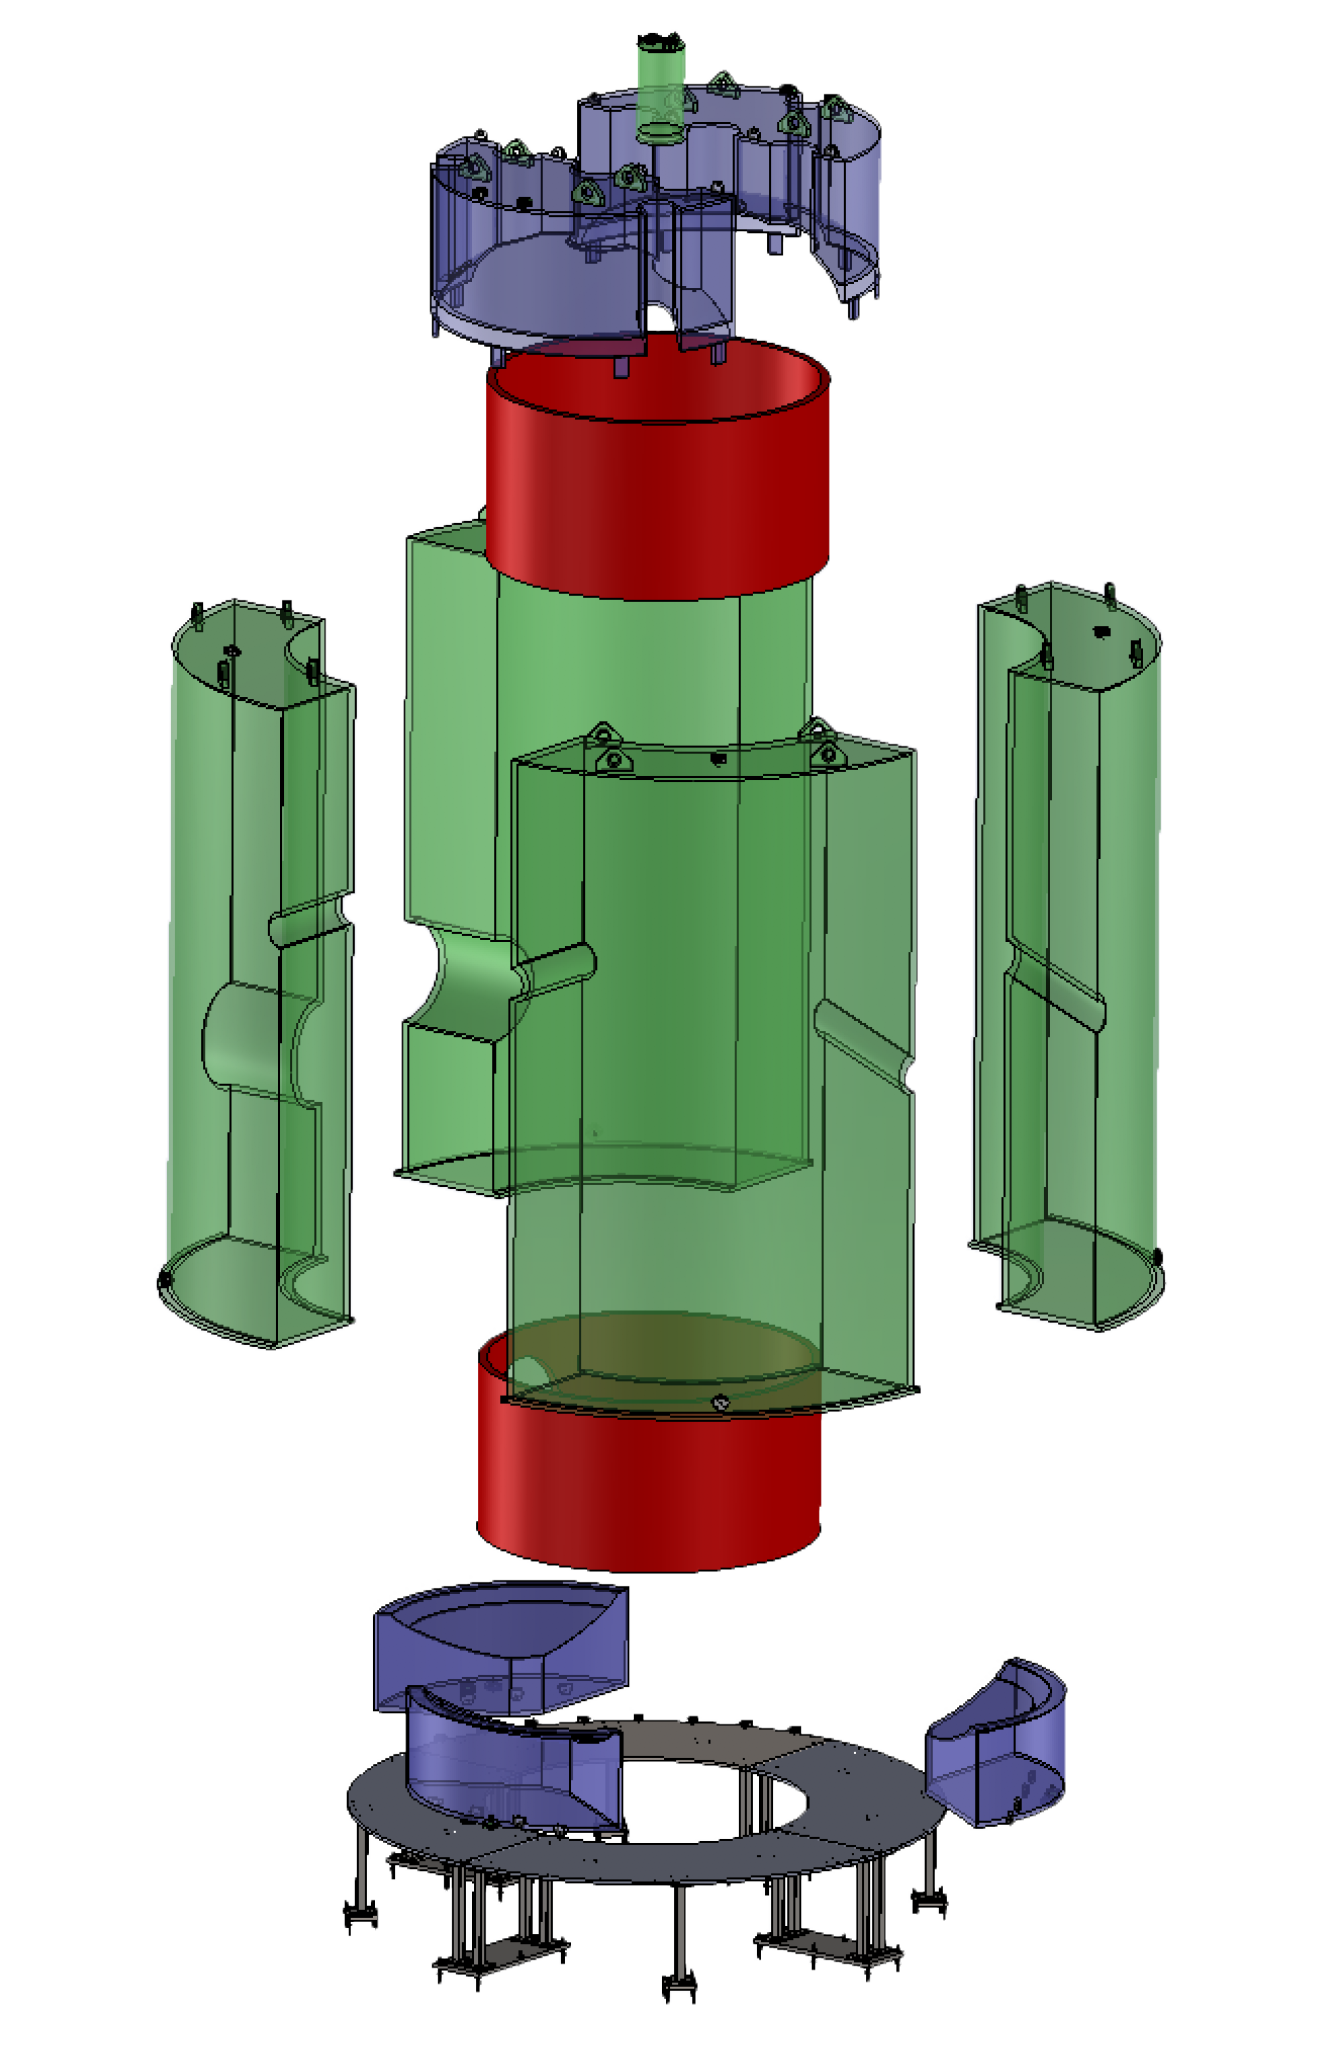
\includegraphics[height=10cm]{Figures/LZ/OD_Tanks_CAD.png}
    \caption{Exploded view of the OD acrylic tanks.}
    \label{fig:LZ_OD_Tanks}
\end{figure}

\par
The tanks are filled with a Gadolinium-doped Liquid Scintillator (GdLS).

linear akylbenze (LAB) as the liquid scintillator.
This is doped with 0.1\% by mass (0.23 - 0.34\% by number) Gadolinium.

\par
The GdLS is combined with TMHA (the chelating agent) and dissolved in the LS.
The components of this cocktail are summarised in Table \ref{tab:GdLS_Components}.



In this, neutron capture happens on the hydrogen; $n + p \xrightarrow{} d + \gamma$ with a capture constant of 200$\mu$s \cite{LZ_TechnicalDesignReview_ref}.
The hydrogen capture produces a single 2.2MeV $\gamma$.
\par
The scintillator in the OD is doped with 0.1\% (by mass) by Gadolinium.
This provides 

\begin{enumerate}
    \item cross section 49kb: (61kb for $Gd^{155}$ and 254kb for $Gd^{157}$)
    \item capture energy release: 8536.39keV ($Gd^{155} \xrightarrow{} Gd^{156}$) and 7937.39keV ($Gd^{157} \xrightarrow{} Gd^{158}$)
    \item More released particles (4.7, $\gamma$'s and $e^{-}$)
    \item neutron-capture time = 30$\mu$s
    \item 9000 optical photons per MeV. Not sure where this number has some from
\end{enumerate}

\par
LZ dopes with 0.1\% by mass (0.23 - 0.34\% by number)

\par
In addition to the gadolinium doping, the scintillator is also made up of two wavelength shifters; a primary shifter (or fluor) and a second wavelength shifter.
The fluor is 2,5-diphenyloxazole (PPO); an organic scintillator which converts shorter wavelength light to longer wavelength light. 
This has a spectrum peak at 385nm (UV).
The second wavelength shifter is 1,4-bis(2-methylstyryl(benzene)) (Bis-MSB). 
Bis-MSB absorbs the PPO scintillation and emits with peak of around 410-425nm.
The reason for the second shifter is that the wavelength emitted is absorbed less by the LS and is closer to the PMT response.
Importantly, the absorption length of the GdLS increases from 1m to in excess of 10m in that range - and continues to rise.

\par
The complete chemical components in the GdLS is shown in Table \ref{tab:GdLS_Components}.

\begin{table}[!htbp]
    \centering
    \begin{tabular}{c | c | c | c}
    \hline
    {Component (referred as)} & {Purpose} & {Weight (g/mol)} & {Mass (g)} \\ \hline
    $C_{17.14}H_{28.28}$ (LAB) & n,g & 234.4  & 853.55 \\
    $C_{15}H_{11}NO$ (PPO) & primary wavelength shifter & 221.3 & 3.00 \\
    $C_{24}H_{22}$ (Bis-MSB) & wavelength shifter & 310.4 & 0.015 \\
    $C_{9}H_{17}O^{-}_{2}$ (TMHA) & chelation agent & 157.2 & 2.58 \\
    natural gadolinium (Gd) & neutron capture & 157.3 & 0.86 
    \end{tabular}
    \caption{Components in 1L of GdLS}
    \label{tab:GdLS_Components}
\end{table} 

\par
Table \ref{tab:Gadolinium_abundances_and_crosssections} contains the natural abundances of gadolinium.

\begin{table}[!htbp]
    \centering
    \begin{tabular}{c | c | c}
    \hline
    {Isotope} & {Abundance (\%)} & {Cross-section (b)} \\ \hline
    $Gd^{152}$ & 0.2 & 735 \\
    $Gd^{154}$ & 2.18 & 85 \\
    $Gd^{155}$ & 14.80 & 60900 \\
    $Gd^{156}$ & 20.47 & 1.8 \\
    $Gd^{157}$ & 15.65 & 254000 \\
    $Gd^{158}$ & 24.84 & 2.2 \\
    $Gd^{160}$ & 21.86 & 1.4

    \end{tabular}
    \caption{Gadolinium natural abundances and thermal neutron capture cross-sections \cite{Gadolinium_abundances_and_crosssection_ref}}
    \label{tab:Gadolinium_abundances_and_crosssections}
\end{table} 

\paragraph{Other Properties}
It is also worth noting that proton scatters and $\alpha$'s have quenched scintillation signals.
For the proton, it is most easily described by the effect of neutron collisions.

\par
In the lab-frame, the ratio between a neutrons initial energy ($E$) and final energy ($E'$) when colliding with an at rest nucleus of mass A follows;
\begin{equation}
    \frac{E'}{E} = \frac{A^2 + 1 + 2A\cos{\theta}}{(A + 1)^2}
\end{equation}
where $\theta$ is the scattering angle in the CoM.
Now, if the nucleus is a hard sphere, so independent of $\theta$, then an elastic scatter follows
\begin{equation}
    E^{'} = E(\frac{A-1}{1})^{2}
\end{equation}
If A = 1 (so is a proton), then it reduces further to $E^{'} = \frac{1}{2}E$, meaning that the neutron loses half its energy on average.
The scattered proton has energy $E - E^{'}$ and is quenched.



\subsection{Neutrons in GdLS}

\subsubsection{background neutrons}
\par
Maybe this and DD neutrons into a separate section before GdLS section?

\subsubsection{DD neutrons}
\par
10,000 DD simulations have been done - a mono-energetic neutron source which LZ will be using for calibration purposes.
Neutrons are emitted at 2.45MeV.

\par
From these simulations (performed on BACCARAT release 6.2.1).
Table \ref{tab:Where_neutrons_go} shows the number neutrons which enter the scintillator and have their final stage there.
The vast majority of the neutrons emitted enter and are captured in the parts of the detector immediately surrounding where it originated.
Importantly, only 23\% of neutrons which remain in the detector finish in the scintillator.
This could be Gd-capture, H-capture, or something else.

\begin{table}[!htbp]
    \centering
    \begin{tabular}{c | c | c  }
    \hline
    {Final Volume}  & {Where all go (\%)} & {Where all go - ignoring OutOfWorld (\%)} \\ \hline
    WaterAndPMTs & 33.59 & 42.55 \\
    OutOfWorld & 21.06 & - \ \\
    ScintillatorCenter & 18.75 & 23.75 \\
    PVCNeutronTube & 15.06 & 19.08 \\
    LiquidXenonTarget & 2.39 & 3.03 \\
    ScintillatorTank & 2.16 & 2.74 \\
    OuterTitaniumVessel & 1.93 & 2.44 \\
    LiquidSkinXenon & 1.27 & 1.61 \\
    InnerTitaniumVessel & 1.19 & 1.51 \\
    WaterTank & 1.12 & 1.42 \\
    SteelNeutronTubeCaps & 0.8 & 1.01 \\
    Other & 0.68 & 0.86 
    \end{tabular}
    \caption{The volume within the detector where DD neutrons have their final step. OutOfWorld indicates that the neutron left the detector area and so the simulation stopped as it's path is not relevant. Other refers to any other part of the detector.}
    \label{tab:Where_neutrons_go}
\end{table} 

\par
Focusing on the neutrons which finish in the scintillator volume, we can in Table \ref{tab:Where_gdls_neutrons_go} that 78\% of neutrons which enter the GdLS end there.
However, it is also interesting to note that 702 neutrons (37\%) enter the scintillator, then leave the scintillator, then enter again (and then die there).

\begin{table}[!htbp]
    \centering
    \begin{tabular}{c | c | c | c }
    \hline
    {Neutron Description}  & {Raw Number} & {Percentage (\%)} & {Percentage remaining in detector (\%)} \\ \hline
    Enters GdLS            &     2406     & 24.06                           & 30.4788 \\
    Dies in GdLS           &     1875     & 18.75                           & 23.7522 \\
    Enters and Dies        &     1875     & 77.9302                         & 77.9302
    
    \end{tabular}
    \caption{What happens to neutrons which enter the scintillator volume.}
    \label{tab:Where_gdls_neutrons_go}
\end{table} 

\par
Figure \ref{fig:dd_neutron_gdls_kinetic_energy_vs_number_of_interactions} shows that on average a neutron will have 27 interactions in the scintillator (excluding transportation steps).

%\pgfplotsset{
%  /pgfplots/colormap={coldredux}{
%    [1cm]
%    rgb255(0cm)=(255,255,255)
%    rgb255(1cm)=(0,192,255)
%    rgb255(3cm)=(0,0,255)
%    rgb255(6cm)=(0,0,0)
%  }
%}

\begin{figure}[!htbp]%
\centering
\begin{tikzpicture}
\centering
  \begin{axis}[%point meta max=150,
    %point meta min=0.0,
    view={0}{90},
    ylabel={Kinetic Energy (MeV)},
    xlabel={Number of Interactions},
    colorbar,
    colorbar style={ylabel={Count}},
    ]
    \addplot3[
      surf,
      shader=flat corner,
      mesh/cols=51,
      mesh/ordering=rowwise,
      point meta = {z<1 ? nan : z}
    ] file {Data/GdLS_Physics/Pre_Capture/dd_neutrons_gdls_initial_keV_vs_n_interactions.txt};
\end{axis}
\end{tikzpicture}
\caption{The relationship between the number of interactions a neutron has in the scintillator and the neutrons kinetic energy when it enters the liquid scintillator volume for neutrons which are 'captured' in the scintillator volume.
}
\label{fig:dd_neutron_gdls_kinetic_energy_vs_number_of_interactions}
\end{figure}


\begin{figure}[!htbp]%
\centering
\begin{tikzpicture}
\centering
  \begin{axis}[%point meta max=150,
    %point meta min=0.0,
    view={0}{90},
    ylabel={Distance before capture (mm)},
    xlabel={Number of Interactions},
    colorbar,
    colorbar style={ylabel={Count}},]
    \addplot3[
      surf,
      shader=flat corner,
      mesh/cols=119,
      mesh/ordering=rowwise,
      point meta = {z<1 ? nan : z}
    ] file {Data/GdLS_Physics/Pre_Capture/dd_neutrons_gdls_distance_travelled_vs_n_interactions.txt};
\end{axis}
\end{tikzpicture}
\caption{The relationship between the number of interactions a neutron has in the scintillator and the neutrons kinetic energy when it enters the liquid scintillator volume for neutrons which are 'captured' in the scintillator volume.
}
\label{fig:dd_neutron_gdls_distance_vs_number_of_interactions}
\end{figure}



\par
Plots to do:

\begin{itemize}
    \item time before capture
    \item captured on what (hydrogen or Gd)
    \item time vs kinE
    \item distance vs kinE
    \item fraction captured by Gd vs H
\end{itemize}


\subsection{Gd Neutron Capture}
\par
After the neutron capture the gadolinium enters an excited state. 
For $Gd^{156}$ this is 8536.39keV and for $Gd^{158}$ is 7937.39keV.
This energy is released as follows;

\begin{enumerate}
    \item Via gamma-rays emission from the decay of an excited nucleus
    \item Internal conversion which leads to
    \begin{enumerate}
        \item auger electron emission
        \item characteristic x-ray emission
    \end{enumerate}
\end{enumerate}


\subsubsection{Dicebox Simulations}
\par
Geant4 is unable so accurately simulate accurately some $\gamma$-decay from excited nuclei.
LUX-ZELPIN circumvented this by using DICEBOX - a monte-carlo package for simulating these decays.
Given that $Gd^{155}$ and $Gd^{157}$ have the largest cross sections and together account for 30\% of abundance, only those were simulated.
The results of these simulations are summarised in this section, and are selected randomly during LZ simulations.
The simulation process performed by LZ collaborators can be found in \cite{ucsb_gdls_dicebox_simulations_ref}.

\par
Figure \ref{fig:Gd_capture_resulting_particle_count} shows the number of discrete packets of energy over which the energy is released after the capture.
The mean value of this (from the 10 million simulations) is 4.654 and 4.754 for $Gd^{156}$ and $Gd^{158}$ respectively.
This is why it is often quoted that the neutron capture releases 4.7 $\gamma$'s.

\begin{figure}[!htbp]
    \centering
    \begin{tikzpicture}
        \begin{axis}[title=N. de-excitation energy transition steps from Gadolinium neutron captures,
            xlabel=N. Steps,
            ylabel=,
            width=15cm,
            height=6cm,
            xmin=0,
            xmax=13,
            ymin=0,
            legend pos=north east,]
            \addplot[red, const plot]
                    table [x=Lower,y=Weight]
                    {Data/GdLS_Physics/DICEBOX/gd156_n_steps.txt};
                \addlegendentry{$Gd^{156}$};
            \addplot[blue, const plot]
                    table [x=Lower,y=Weight]
                    {Data/GdLS_Physics/DICEBOX/gd158_n_steps.txt};
                \addlegendentry{$Gd^{158}$};
        \end{axis}
    \end{tikzpicture}
    \caption{Result of 10 million DICEBOX simulations (5 million of both $Gd^{155}$ and $Gd^{157}$) showing in how many stages the energy is released from the atom.}
    \label{fig:Gd_capture_resulting_particle_count}
\end{figure}

\par
The simulation encompasses both $\gamma$-emission from the nucleus directly as well as the transfer of energy to an electron (internal conversion).
Where the energy goes within the atom is shown in Table \ref{tab:Gd_internal_energy_conversion}.
It shows that there is also a gamma emitted and that roughly 30\% of the time only $\gamma$'s are emitted, however it is most likely that energy is also passed to a shell electron.
From this, we can conclude that the dominant emission from the neutron capture are $\gamma$'s, with auger electrons and x-rays comprising a much smaller percentage of the emission.
\par
A less useful Figure is Figure \ref{fig:Gd_capture_energy_conversion_shells} shows where the energy goes in terms of electron shells. 

\begin{table}[!htbp]
    \centering
    \begin{tabular}{c | c | c | c | c | c | c}
    \hline
    {Excited Isotope}  & {$\gamma$-only} & {$\gamma$ + 1$e^{-}$} & {$\gamma$ + 2$e^{-}$} & {$\gamma$ + 3$e^{-}$} & {$\gamma$ + 4$e^{-}$+} & {$e^{-}$-only}\\ \hline
    $Gd^{156}$         & 29.8055         & 65.1064               & 5.00976               & 0.07648               & 0.00186               & 0.0        \\
    $Gd^{158}$         & 26.8031         & 67.0329               & 6.09488               & 0.06848               & 0.00064               & 0.0
     
    \end{tabular}
    \caption{Gadolinium nuclei de-excitation path by percentage. In this table, $e^{-}$ refer internal conversion, when the nucleus transfers energy to a shell electron.}
    \label{tab:Gd_internal_energy_conversion}
\end{table} 

\begin{figure}[!htbp]
    \centering
    \begin{tikzpicture}
        \begin{axis}[title=Fraction of steps going to internal conversion vs directly to $\gamma$'s,
            xlabel=Energy Transfer location,
            ylabel=Percentage of steps,
            width=15cm,
            height=6cm,
            legend pos=north east,
            xtick=data,
            xticklabels from table={Data/GdLS_Physics/DICEBOX/gd158_energy_conversion_to_shells.txt}{Label}]
            \addplot[red, const plot]
                    table [x=Bins, y=Weight]
                    {Data/GdLS_Physics/DICEBOX/gd158_energy_conversion_to_shells.txt};
                \addlegendentry{$Gd^{156}$};
            \addplot[blue, const plot]
                    table [x=Bins, y=Weight]
                    {Data/GdLS_Physics/DICEBOX/gd156_energy_conversion_to_shells.txt};
                \addlegendentry{$Gd^{158}$};
        \end{axis}
    \end{tikzpicture}
    \caption{DICEBOX simulation showing where the energy goes. On average each excited nucleus transfers it's energy in 4.7 steps, so the majority of the energy is transferred to $\gamma$'s. This figure isn't actually that helpful.}
    \label{fig:Gd_capture_energy_conversion_shells}
\end{figure}

\par
The proportion of the energy transferred directly to $\gamma$'s vs via internal conversion is shown in Figure \ref{fig:Gd_deexcitation_energy_fractions}.

\begin{figure}[!htbp]%
\centering
\begin{tikzpicture}
\centering
  \begin{groupplot}[view={0}{90},
    group style = {group size = 2 by 1}]
    \nextgroupplot[
    xmin=0,
    xmax=100,
    ymode=log,
    xlabel={Percentage of Energy (\%)},
    ylabel={Count},]
    \addplot[ybar interval, red, const plot]
            table [x=Lower,y=Weight]
            {Data/GdLS_Physics/DICEBOX/gd156_energy_fraction_gamma.txt};
    \addlegendentry{$Gd^{156}$-$\gamma$};
    \addplot[ybar interval, blue, const plot]
                    table [x=Lower,y=Weight]
                    {Data/GdLS_Physics/DICEBOX/gd156_energy_fraction_electron.txt};
    \addlegendentry{$Gd^{156}$-IC};
    \nextgroupplot[
    xmin=0,
    xmax=100,
    ymode=log,
    xlabel={Percentage of Energy (\%)}]
    \addplot[ybar interval, red, const plot]
            table [x=Lower,y=Weight]
            {Data/GdLS_Physics/DICEBOX/gd158_energy_fraction_gamma.txt};
    \addlegendentry{$Gd^{156}$-$\gamma$};
    \addplot[ybar interval, blue, const plot]
                    table [x=Lower,y=Weight]
                    {Data/GdLS_Physics/DICEBOX/gd158_energy_fraction_electron.txt};
    \addlegendentry{$Gd^{156}$-IC};
  \end{groupplot}
\end{tikzpicture}
\caption{The fraction of energy from the excited nucleus which goes to $\gamma$'s and to internval conversion.
\textbf{Left:} $Gd^{156}$ de-excitation path.
\textbf{Right:} $Gd^{158}$ de-excitation path.
}
\label{fig:Gd_deexcitation_energy_fractions}
\end{figure}




\par
Given what has been determined above, it is worth looking at the $\gamma$ spectrum, shown in Figure \ref{fig:Gd_capture_resulting_gamma_spectrum}.


\begin{figure}[!htbp]
    \centering
    \begin{tikzpicture}
        \begin{axis}[title=$\gamma$ energy spectrum from $Gd^{155}$ and $Gd^{157}$ neutron captures,
            xlabel=Energy (KeV),
            ylabel=,
            width=15cm,
            height=6cm,
            xmin=0,
            xmax=8000,
            ymin=0,
            legend pos=north east,]
            \addplot[red, const plot]
                    table [x=Lower,y=Weight]
                    {Data/GdLS_Physics/DICEBOX/gd156_gamma_spectrum.txt};
                \addlegendentry{$Gd^{156}$};
            \addplot[blue, const plot]
                    table [x=Lower,y=Weight]
                    {Data/GdLS_Physics/DICEBOX/gd158_gamma_spectrum.txt};
                \addlegendentry{$Gd^{158}$};
        \end{axis}
    \end{tikzpicture}
    \caption{DICEBOX simulation of the energy released by $\gamma$'s from nuclei de-excitation after neutron capture, going from $Gd^{155} \xrightarrow{} Gd^{156}$ or $Gd^{157} \xrightarrow{} Gd^{158}$}
    \label{fig:Gd_capture_resulting_gamma_spectrum}
\end{figure}


\begin{figure}
	\begin{tikzpicture}
		\centering
		\begin{axis}[%point meta max=150,
			%point meta min=0.0,
			view={0}{90},
			ylabel={Cross-Section (barns)},
			xlabel={Incident Energy (MeV)},
			width=15cm,
			height=8cm,
			ymode=log,
			xmode=log,
			]
			\addplot[blue] table[x=energy,y=barns] {Data/GdLS_Physics/capture_cross_sections/h.dat};
			\addplot[orange] table[x=energy,y=barns] {Data/GdLS_Physics/capture_cross_sections/gd155.dat};
			\addplot[green] table[x=energy,y=barns] {Data/GdLS_Physics/capture_cross_sections/gd157.dat};
			\legend{H, ${}^{155}$Gd, ${}^{157}$Gd};
		\end{axis}
	\end{tikzpicture}
\caption{Capture cross sections for the most significant capture particles in GdLS cocktail. 
A neutron has an increase capture probability if it's energy is close to that of the isotope energy. 
Values from ENDF/B-VIII.0 \cite{endf_bv3_ref}.}
\label{fig:gdls_capture_cross_sections}
\end{figure}
		



\section{Released Particles}
\par
The particles released as a result of the neutron capture ($\gamma$'s and $e^{-}$'s) then follow Birk's law, shown in equation \ref{eq:birkslaw}.

\begin{equation}
    \frac{dL}{dx} = S \frac{\frac{dE}{dx}}{1 + k_{B}\frac{dE}{dx} + C\frac{dE}{dx}^2}
    \label{eq:birkslaw}
\end{equation}
Here, L is the the light yield, S is the scintillation efficiency, $\frac{dE}{dx}$ is the energy loss of the particle per path length, and $k_{B}$ and $C$ are Birk's law parameters.
The parameters for GdLS are shown in table \ref{tab:Birks_law_parameters}.


\begin{table}[!htbp]
    \centering
    \begin{tabular}{c | c | c | c }
                   & S (photons/MeV) & $k_{B}$ & $C$ \\ \hline
    $\alpha$       &                 & 4.63E-3 & 1.77E-6 \\
    $\beta/\gamma$ & 9,000           & 0.03    & 0 \\ 
    proton         &                 & 8.26E-3 & 0
    \end{tabular}
    \caption{GdLS parameters for Birk's law}
    \label{tab:Birks_law_parameters}
\end{table} 

\begin{itemize}
    \item electron time + distance + n. interactions
    \item gamma time + distance + n. interactions
    \item N. optical photons per gamma
    \item N. optical photons per electron
    \item time between first and last optical photon from capture
\end{itemize}

\subsection{gammas}
\par
What happens to gammas



\subsection{electrons}
\par
What happens to electrons


\subsection{optical photons}
\par
Ultimately all of these result in optical photons will propagate until they are absorbed at a surface.
In order to be detected, the optical photons must be absorbed by a PMT, causing a photoelectron cascade.
This however adds an additional 

\begin{tcolorbox}[colback=red!5!white, colframe=red!50!black, title=Key Plots]
\begin{enumerate}
    \item Light Collection Efficiency
    \item PMT QE
    \item GdLS light output
\end{enumerate}
\end{tcolorbox}


\begin{figure}[!htbp]%
\centering
\begin{tikzpicture}
\centering
  \begin{groupplot}[%view={0}{90},
    group style = {group size = 2 by 1}]
    \nextgroupplot[
    xmin=300,
    xmax=600,
    ylabel={Emission (Arbitrary Units)},]
    \addplot[ybar interval, blue, const plot]
                    table [x=Wavelength,y=Rate]
                    {Data/GdLS_Physics/Light_Collection/gdls_light_output.dat};
    \nextgroupplot[
    xmin=300,
    xmax=600,
    xlabel={Wavelength (nm)},
    ylabel={QE},
    yticklabel pos=right,]
    \addplot[ybar interval, red, const plot]
            table [x=Wavelength,y=QE]
            {Data/GdLS_Physics/Light_Collection/od_pmt_qe.dat};
  \end{groupplot}
\end{tikzpicture}
\caption{Primary OD detection properties. 
\textbf{Left:} Light 
\textbf{Right:} PMT QE
}
\label{fig:od_detection_properties}
\end{figure}


\begin{figure}[!htbp]
\centering
\resizebox{\textwidth}{!}{
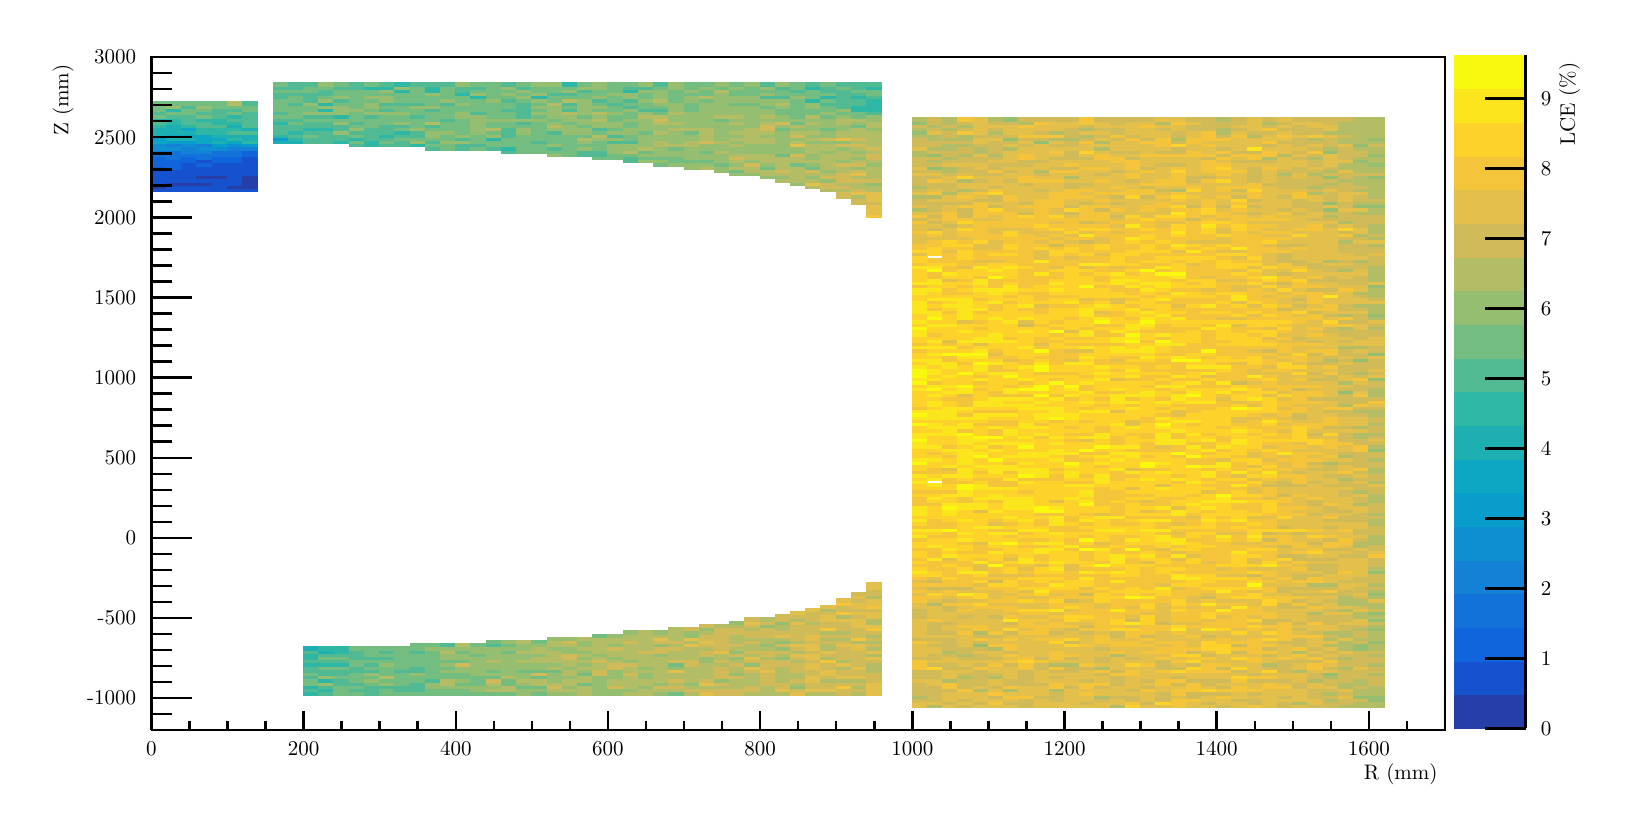
\begin{tikzpicture}
\pgfdeclareplotmark{cross} {
\pgfpathmoveto{\pgfpoint{-0.3\pgfplotmarksize}{\pgfplotmarksize}}
\pgfpathlineto{\pgfpoint{+0.3\pgfplotmarksize}{\pgfplotmarksize}}
\pgfpathlineto{\pgfpoint{+0.3\pgfplotmarksize}{0.3\pgfplotmarksize}}
\pgfpathlineto{\pgfpoint{+1\pgfplotmarksize}{0.3\pgfplotmarksize}}
\pgfpathlineto{\pgfpoint{+1\pgfplotmarksize}{-0.3\pgfplotmarksize}}
\pgfpathlineto{\pgfpoint{+0.3\pgfplotmarksize}{-0.3\pgfplotmarksize}}
\pgfpathlineto{\pgfpoint{+0.3\pgfplotmarksize}{-1.\pgfplotmarksize}}
\pgfpathlineto{\pgfpoint{-0.3\pgfplotmarksize}{-1.\pgfplotmarksize}}
\pgfpathlineto{\pgfpoint{-0.3\pgfplotmarksize}{-0.3\pgfplotmarksize}}
\pgfpathlineto{\pgfpoint{-1.\pgfplotmarksize}{-0.3\pgfplotmarksize}}
\pgfpathlineto{\pgfpoint{-1.\pgfplotmarksize}{0.3\pgfplotmarksize}}
\pgfpathlineto{\pgfpoint{-0.3\pgfplotmarksize}{0.3\pgfplotmarksize}}
\pgfpathclose
\pgfusepathqstroke
}
\pgfdeclareplotmark{cross*} {
\pgfpathmoveto{\pgfpoint{-0.3\pgfplotmarksize}{\pgfplotmarksize}}
\pgfpathlineto{\pgfpoint{+0.3\pgfplotmarksize}{\pgfplotmarksize}}
\pgfpathlineto{\pgfpoint{+0.3\pgfplotmarksize}{0.3\pgfplotmarksize}}
\pgfpathlineto{\pgfpoint{+1\pgfplotmarksize}{0.3\pgfplotmarksize}}
\pgfpathlineto{\pgfpoint{+1\pgfplotmarksize}{-0.3\pgfplotmarksize}}
\pgfpathlineto{\pgfpoint{+0.3\pgfplotmarksize}{-0.3\pgfplotmarksize}}
\pgfpathlineto{\pgfpoint{+0.3\pgfplotmarksize}{-1.\pgfplotmarksize}}
\pgfpathlineto{\pgfpoint{-0.3\pgfplotmarksize}{-1.\pgfplotmarksize}}
\pgfpathlineto{\pgfpoint{-0.3\pgfplotmarksize}{-0.3\pgfplotmarksize}}
\pgfpathlineto{\pgfpoint{-1.\pgfplotmarksize}{-0.3\pgfplotmarksize}}
\pgfpathlineto{\pgfpoint{-1.\pgfplotmarksize}{0.3\pgfplotmarksize}}
\pgfpathlineto{\pgfpoint{-0.3\pgfplotmarksize}{0.3\pgfplotmarksize}}
\pgfpathclose
\pgfusepathqfillstroke
}
\pgfdeclareplotmark{newstar} {
\pgfpathmoveto{\pgfqpoint{0pt}{\pgfplotmarksize}}
\pgfpathlineto{\pgfqpointpolar{44}{0.5\pgfplotmarksize}}
\pgfpathlineto{\pgfqpointpolar{18}{\pgfplotmarksize}}
\pgfpathlineto{\pgfqpointpolar{-20}{0.5\pgfplotmarksize}}
\pgfpathlineto{\pgfqpointpolar{-54}{\pgfplotmarksize}}
\pgfpathlineto{\pgfqpointpolar{-90}{0.5\pgfplotmarksize}}
\pgfpathlineto{\pgfqpointpolar{234}{\pgfplotmarksize}}
\pgfpathlineto{\pgfqpointpolar{198}{0.5\pgfplotmarksize}}
\pgfpathlineto{\pgfqpointpolar{162}{\pgfplotmarksize}}
\pgfpathlineto{\pgfqpointpolar{134}{0.5\pgfplotmarksize}}
\pgfpathclose
\pgfusepathqstroke
}
\pgfdeclareplotmark{newstar*} {
\pgfpathmoveto{\pgfqpoint{0pt}{\pgfplotmarksize}}
\pgfpathlineto{\pgfqpointpolar{44}{0.5\pgfplotmarksize}}
\pgfpathlineto{\pgfqpointpolar{18}{\pgfplotmarksize}}
\pgfpathlineto{\pgfqpointpolar{-20}{0.5\pgfplotmarksize}}
\pgfpathlineto{\pgfqpointpolar{-54}{\pgfplotmarksize}}
\pgfpathlineto{\pgfqpointpolar{-90}{0.5\pgfplotmarksize}}
\pgfpathlineto{\pgfqpointpolar{234}{\pgfplotmarksize}}
\pgfpathlineto{\pgfqpointpolar{198}{0.5\pgfplotmarksize}}
\pgfpathlineto{\pgfqpointpolar{162}{\pgfplotmarksize}}
\pgfpathlineto{\pgfqpointpolar{134}{0.5\pgfplotmarksize}}
\pgfpathclose
\pgfusepathqfillstroke
}
\definecolor{c}{rgb}{1,1,1};
\draw [color=c, fill=c] (0,0) rectangle (20,9.91803);
\draw [color=c, fill=c] (1.56401,1.00281) rectangle (17.9931,9.55115);
\definecolor{c}{rgb}{0,0,0};
\draw [c,line width=0.9] (1.56401,1.00281) -- (1.56401,9.55115) -- (17.9931,9.55115) -- (17.9931,1.00281) -- (1.56401,1.00281);
\definecolor{c}{rgb}{1,1,1};
\draw [color=c, fill=c] (1.56401,1.00281) rectangle (17.9931,9.55115);
\definecolor{c}{rgb}{0,0,0};
\draw [c,line width=0.9] (1.56401,1.00281) -- (1.56401,9.55115) -- (17.9931,9.55115) -- (17.9931,1.00281) -- (1.56401,1.00281);
\definecolor{c}{rgb}{0.884975,0.752825,0.292488};
\draw [color=c, fill=c] (11.2282,1.28775) rectangle (11.4215,1.32846);
\definecolor{c}{rgb}{0.701397,0.739462,0.397147};
\draw [color=c, fill=c] (11.4215,1.28775) rectangle (11.6147,1.32846);
\definecolor{c}{rgb}{0.884975,0.752825,0.292488};
\draw [color=c, fill=c] (11.6147,1.28775) rectangle (11.808,1.32846);
\definecolor{c}{rgb}{0.8186,0.7328,0.3499};
\draw [color=c, fill=c] (11.808,1.28775) rectangle (12.0013,1.32846);
\definecolor{c}{rgb}{0.884975,0.752825,0.292488};
\draw [color=c, fill=c] (12.0013,1.28775) rectangle (12.1946,1.32846);
\draw [color=c, fill=c] (12.1946,1.28775) rectangle (12.3879,1.32846);
\draw [color=c, fill=c] (12.3879,1.28775) rectangle (12.5812,1.32846);
\definecolor{c}{rgb}{0.8186,0.7328,0.3499};
\draw [color=c, fill=c] (12.5812,1.28775) rectangle (12.7744,1.32846);
\definecolor{c}{rgb}{0.884975,0.752825,0.292488};
\draw [color=c, fill=c] (12.7744,1.28775) rectangle (12.9677,1.32846);
\draw [color=c, fill=c] (12.9677,1.28775) rectangle (13.161,1.32846);
\draw [color=c, fill=c] (13.161,1.28775) rectangle (13.3543,1.32846);
\draw [color=c, fill=c] (13.3543,1.28775) rectangle (13.5476,1.32846);
\draw [color=c, fill=c] (13.5476,1.28775) rectangle (13.7409,1.32846);
\definecolor{c}{rgb}{0.701397,0.739462,0.397147};
\draw [color=c, fill=c] (13.7409,1.28775) rectangle (13.9341,1.32846);
\definecolor{c}{rgb}{0.992,0.823138,0.170006};
\draw [color=c, fill=c] (13.9341,1.28775) rectangle (14.1274,1.32846);
\definecolor{c}{rgb}{0.884975,0.752825,0.292488};
\draw [color=c, fill=c] (14.1274,1.28775) rectangle (14.3207,1.32846);
\draw [color=c, fill=c] (14.3207,1.28775) rectangle (14.514,1.32846);
\definecolor{c}{rgb}{0.956881,0.774519,0.230291};
\draw [color=c, fill=c] (14.514,1.28775) rectangle (14.7073,1.32846);
\definecolor{c}{rgb}{0.884975,0.752825,0.292488};
\draw [color=c, fill=c] (14.7073,1.28775) rectangle (14.9005,1.32846);
\draw [color=c, fill=c] (14.9005,1.28775) rectangle (15.0938,1.32846);
\definecolor{c}{rgb}{0.8186,0.7328,0.3499};
\draw [color=c, fill=c] (15.0938,1.28775) rectangle (15.2871,1.32846);
\definecolor{c}{rgb}{0.884975,0.752825,0.292488};
\draw [color=c, fill=c] (15.2871,1.28775) rectangle (15.4804,1.32846);
\definecolor{c}{rgb}{0.956881,0.774519,0.230291};
\draw [color=c, fill=c] (15.4804,1.28775) rectangle (15.6737,1.32846);
\definecolor{c}{rgb}{0.884975,0.752825,0.292488};
\draw [color=c, fill=c] (15.6737,1.28775) rectangle (15.867,1.32846);
\definecolor{c}{rgb}{0.8186,0.7328,0.3499};
\draw [color=c, fill=c] (15.867,1.28775) rectangle (16.0602,1.32846);
\definecolor{c}{rgb}{0.884975,0.752825,0.292488};
\draw [color=c, fill=c] (16.0602,1.28775) rectangle (16.2535,1.32846);
\definecolor{c}{rgb}{0.8186,0.7328,0.3499};
\draw [color=c, fill=c] (16.2535,1.28775) rectangle (16.4468,1.32846);
\draw [color=c, fill=c] (16.4468,1.28775) rectangle (16.6401,1.32846);
\definecolor{c}{rgb}{0.701397,0.739462,0.397147};
\draw [color=c, fill=c] (16.6401,1.28775) rectangle (16.8334,1.32846);
\draw [color=c, fill=c] (16.8334,1.28775) rectangle (17.0267,1.32846);
\draw [color=c, fill=c] (17.0267,1.28775) rectangle (17.2199,1.32846);
\definecolor{c}{rgb}{0.884975,0.752825,0.292488};
\draw [color=c, fill=c] (11.2282,1.32846) rectangle (11.4215,1.36917);
\draw [color=c, fill=c] (11.4215,1.32846) rectangle (11.6147,1.36917);
\definecolor{c}{rgb}{0.8186,0.7328,0.3499};
\draw [color=c, fill=c] (11.6147,1.32846) rectangle (11.808,1.36917);
\definecolor{c}{rgb}{0.884975,0.752825,0.292488};
\draw [color=c, fill=c] (11.808,1.32846) rectangle (12.0013,1.36917);
\definecolor{c}{rgb}{0.8186,0.7328,0.3499};
\draw [color=c, fill=c] (12.0013,1.32846) rectangle (12.1946,1.36917);
\definecolor{c}{rgb}{0.956881,0.774519,0.230291};
\draw [color=c, fill=c] (12.1946,1.32846) rectangle (12.3879,1.36917);
\definecolor{c}{rgb}{0.8186,0.7328,0.3499};
\draw [color=c, fill=c] (12.3879,1.32846) rectangle (12.5812,1.36917);
\draw [color=c, fill=c] (12.5812,1.32846) rectangle (12.7744,1.36917);
\definecolor{c}{rgb}{0.884975,0.752825,0.292488};
\draw [color=c, fill=c] (12.7744,1.32846) rectangle (12.9677,1.36917);
\draw [color=c, fill=c] (12.9677,1.32846) rectangle (13.161,1.36917);
\draw [color=c, fill=c] (13.161,1.32846) rectangle (13.3543,1.36917);
\definecolor{c}{rgb}{0.8186,0.7328,0.3499};
\draw [color=c, fill=c] (13.3543,1.32846) rectangle (13.5476,1.36917);
\definecolor{c}{rgb}{0.884975,0.752825,0.292488};
\draw [color=c, fill=c] (13.5476,1.32846) rectangle (13.7409,1.36917);
\draw [color=c, fill=c] (13.7409,1.32846) rectangle (13.9341,1.36917);
\definecolor{c}{rgb}{0.956881,0.774519,0.230291};
\draw [color=c, fill=c] (13.9341,1.32846) rectangle (14.1274,1.36917);
\definecolor{c}{rgb}{0.8186,0.7328,0.3499};
\draw [color=c, fill=c] (14.1274,1.32846) rectangle (14.3207,1.36917);
\definecolor{c}{rgb}{0.992,0.823138,0.170006};
\draw [color=c, fill=c] (14.3207,1.32846) rectangle (14.514,1.36917);
\definecolor{c}{rgb}{0.956881,0.774519,0.230291};
\draw [color=c, fill=c] (14.514,1.32846) rectangle (14.7073,1.36917);
\definecolor{c}{rgb}{0.884975,0.752825,0.292488};
\draw [color=c, fill=c] (14.7073,1.32846) rectangle (14.9005,1.36917);
\definecolor{c}{rgb}{0.8186,0.7328,0.3499};
\draw [color=c, fill=c] (14.9005,1.32846) rectangle (15.0938,1.36917);
\definecolor{c}{rgb}{0.884975,0.752825,0.292488};
\draw [color=c, fill=c] (15.0938,1.32846) rectangle (15.2871,1.36917);
\draw [color=c, fill=c] (15.2871,1.32846) rectangle (15.4804,1.36917);
\definecolor{c}{rgb}{0.8186,0.7328,0.3499};
\draw [color=c, fill=c] (15.4804,1.32846) rectangle (15.6737,1.36917);
\definecolor{c}{rgb}{0.884975,0.752825,0.292488};
\draw [color=c, fill=c] (15.6737,1.32846) rectangle (15.867,1.36917);
\definecolor{c}{rgb}{0.8186,0.7328,0.3499};
\draw [color=c, fill=c] (15.867,1.32846) rectangle (16.0602,1.36917);
\definecolor{c}{rgb}{0.701397,0.739462,0.397147};
\draw [color=c, fill=c] (16.0602,1.32846) rectangle (16.2535,1.36917);
\definecolor{c}{rgb}{0.884975,0.752825,0.292488};
\draw [color=c, fill=c] (16.2535,1.32846) rectangle (16.4468,1.36917);
\definecolor{c}{rgb}{0.8186,0.7328,0.3499};
\draw [color=c, fill=c] (16.4468,1.32846) rectangle (16.6401,1.36917);
\draw [color=c, fill=c] (16.6401,1.32846) rectangle (16.8334,1.36917);
\definecolor{c}{rgb}{0.701397,0.739462,0.397147};
\draw [color=c, fill=c] (16.8334,1.32846) rectangle (17.0267,1.36917);
\draw [color=c, fill=c] (17.0267,1.32846) rectangle (17.2199,1.36917);
\definecolor{c}{rgb}{0.8186,0.7328,0.3499};
\draw [color=c, fill=c] (11.2282,1.36917) rectangle (11.4215,1.40987);
\draw [color=c, fill=c] (11.4215,1.36917) rectangle (11.6147,1.40987);
\definecolor{c}{rgb}{0.884975,0.752825,0.292488};
\draw [color=c, fill=c] (11.6147,1.36917) rectangle (11.808,1.40987);
\definecolor{c}{rgb}{0.8186,0.7328,0.3499};
\draw [color=c, fill=c] (11.808,1.36917) rectangle (12.0013,1.40987);
\definecolor{c}{rgb}{0.884975,0.752825,0.292488};
\draw [color=c, fill=c] (12.0013,1.36917) rectangle (12.1946,1.40987);
\draw [color=c, fill=c] (12.1946,1.36917) rectangle (12.3879,1.40987);
\draw [color=c, fill=c] (12.3879,1.36917) rectangle (12.5812,1.40987);
\definecolor{c}{rgb}{0.8186,0.7328,0.3499};
\draw [color=c, fill=c] (12.5812,1.36917) rectangle (12.7744,1.40987);
\definecolor{c}{rgb}{0.884975,0.752825,0.292488};
\draw [color=c, fill=c] (12.7744,1.36917) rectangle (12.9677,1.40987);
\definecolor{c}{rgb}{0.8186,0.7328,0.3499};
\draw [color=c, fill=c] (12.9677,1.36917) rectangle (13.161,1.40987);
\definecolor{c}{rgb}{0.884975,0.752825,0.292488};
\draw [color=c, fill=c] (13.161,1.36917) rectangle (13.3543,1.40987);
\draw [color=c, fill=c] (13.3543,1.36917) rectangle (13.5476,1.40987);
\definecolor{c}{rgb}{0.8186,0.7328,0.3499};
\draw [color=c, fill=c] (13.5476,1.36917) rectangle (13.7409,1.40987);
\definecolor{c}{rgb}{0.884975,0.752825,0.292488};
\draw [color=c, fill=c] (13.7409,1.36917) rectangle (13.9341,1.40987);
\definecolor{c}{rgb}{0.8186,0.7328,0.3499};
\draw [color=c, fill=c] (13.9341,1.36917) rectangle (14.1274,1.40987);
\definecolor{c}{rgb}{0.884975,0.752825,0.292488};
\draw [color=c, fill=c] (14.1274,1.36917) rectangle (14.3207,1.40987);
\definecolor{c}{rgb}{0.8186,0.7328,0.3499};
\draw [color=c, fill=c] (14.3207,1.36917) rectangle (14.514,1.40987);
\definecolor{c}{rgb}{0.956881,0.774519,0.230291};
\draw [color=c, fill=c] (14.514,1.36917) rectangle (14.7073,1.40987);
\draw [color=c, fill=c] (14.7073,1.36917) rectangle (14.9005,1.40987);
\definecolor{c}{rgb}{0.884975,0.752825,0.292488};
\draw [color=c, fill=c] (14.9005,1.36917) rectangle (15.0938,1.40987);
\draw [color=c, fill=c] (15.0938,1.36917) rectangle (15.2871,1.40987);
\definecolor{c}{rgb}{0.8186,0.7328,0.3499};
\draw [color=c, fill=c] (15.2871,1.36917) rectangle (15.4804,1.40987);
\draw [color=c, fill=c] (15.4804,1.36917) rectangle (15.6737,1.40987);
\definecolor{c}{rgb}{0.884975,0.752825,0.292488};
\draw [color=c, fill=c] (15.6737,1.36917) rectangle (15.867,1.40987);
\draw [color=c, fill=c] (15.867,1.36917) rectangle (16.0602,1.40987);
\draw [color=c, fill=c] (16.0602,1.36917) rectangle (16.2535,1.40987);
\draw [color=c, fill=c] (16.2535,1.36917) rectangle (16.4468,1.40987);
\definecolor{c}{rgb}{0.701397,0.739462,0.397147};
\draw [color=c, fill=c] (16.4468,1.36917) rectangle (16.6401,1.40987);
\definecolor{c}{rgb}{0.8186,0.7328,0.3499};
\draw [color=c, fill=c] (16.6401,1.36917) rectangle (16.8334,1.40987);
\draw [color=c, fill=c] (16.8334,1.36917) rectangle (17.0267,1.40987);
\definecolor{c}{rgb}{0.584194,0.746125,0.444394};
\draw [color=c, fill=c] (17.0267,1.36917) rectangle (17.2199,1.40987);
\definecolor{c}{rgb}{0.701397,0.739462,0.397147};
\draw [color=c, fill=c] (11.2282,1.40987) rectangle (11.4215,1.45058);
\definecolor{c}{rgb}{0.8186,0.7328,0.3499};
\draw [color=c, fill=c] (11.4215,1.40987) rectangle (11.6147,1.45058);
\definecolor{c}{rgb}{0.884975,0.752825,0.292488};
\draw [color=c, fill=c] (11.6147,1.40987) rectangle (11.808,1.45058);
\draw [color=c, fill=c] (11.808,1.40987) rectangle (12.0013,1.45058);
\draw [color=c, fill=c] (12.0013,1.40987) rectangle (12.1946,1.45058);
\definecolor{c}{rgb}{0.8186,0.7328,0.3499};
\draw [color=c, fill=c] (12.1946,1.40987) rectangle (12.3879,1.45058);
\definecolor{c}{rgb}{0.956881,0.774519,0.230291};
\draw [color=c, fill=c] (12.3879,1.40987) rectangle (12.5812,1.45058);
\draw [color=c, fill=c] (12.5812,1.40987) rectangle (12.7744,1.45058);
\definecolor{c}{rgb}{0.8186,0.7328,0.3499};
\draw [color=c, fill=c] (12.7744,1.40987) rectangle (12.9677,1.45058);
\draw [color=c, fill=c] (12.9677,1.40987) rectangle (13.161,1.45058);
\definecolor{c}{rgb}{0.884975,0.752825,0.292488};
\draw [color=c, fill=c] (13.161,1.40987) rectangle (13.3543,1.45058);
\draw [color=c, fill=c] (13.3543,1.40987) rectangle (13.5476,1.45058);
\definecolor{c}{rgb}{0.701397,0.739462,0.397147};
\draw [color=c, fill=c] (13.5476,1.40987) rectangle (13.7409,1.45058);
\definecolor{c}{rgb}{0.8186,0.7328,0.3499};
\draw [color=c, fill=c] (13.7409,1.40987) rectangle (13.9341,1.45058);
\draw [color=c, fill=c] (13.9341,1.40987) rectangle (14.1274,1.45058);
\definecolor{c}{rgb}{0.884975,0.752825,0.292488};
\draw [color=c, fill=c] (14.1274,1.40987) rectangle (14.3207,1.45058);
\definecolor{c}{rgb}{0.8186,0.7328,0.3499};
\draw [color=c, fill=c] (14.3207,1.40987) rectangle (14.514,1.45058);
\definecolor{c}{rgb}{0.884975,0.752825,0.292488};
\draw [color=c, fill=c] (14.514,1.40987) rectangle (14.7073,1.45058);
\definecolor{c}{rgb}{0.8186,0.7328,0.3499};
\draw [color=c, fill=c] (14.7073,1.40987) rectangle (14.9005,1.45058);
\definecolor{c}{rgb}{0.884975,0.752825,0.292488};
\draw [color=c, fill=c] (14.9005,1.40987) rectangle (15.0938,1.45058);
\definecolor{c}{rgb}{0.956881,0.774519,0.230291};
\draw [color=c, fill=c] (15.0938,1.40987) rectangle (15.2871,1.45058);
\definecolor{c}{rgb}{0.884975,0.752825,0.292488};
\draw [color=c, fill=c] (15.2871,1.40987) rectangle (15.4804,1.45058);
\draw [color=c, fill=c] (15.4804,1.40987) rectangle (15.6737,1.45058);
\draw [color=c, fill=c] (15.6737,1.40987) rectangle (15.867,1.45058);
\definecolor{c}{rgb}{0.8186,0.7328,0.3499};
\draw [color=c, fill=c] (15.867,1.40987) rectangle (16.0602,1.45058);
\definecolor{c}{rgb}{0.884975,0.752825,0.292488};
\draw [color=c, fill=c] (16.0602,1.40987) rectangle (16.2535,1.45058);
\definecolor{c}{rgb}{0.8186,0.7328,0.3499};
\draw [color=c, fill=c] (16.2535,1.40987) rectangle (16.4468,1.45058);
\draw [color=c, fill=c] (16.4468,1.40987) rectangle (16.6401,1.45058);
\definecolor{c}{rgb}{0.884975,0.752825,0.292488};
\draw [color=c, fill=c] (16.6401,1.40987) rectangle (16.8334,1.45058);
\definecolor{c}{rgb}{0.584194,0.746125,0.444394};
\draw [color=c, fill=c] (16.8334,1.40987) rectangle (17.0267,1.45058);
\draw [color=c, fill=c] (17.0267,1.40987) rectangle (17.2199,1.45058);
\definecolor{c}{rgb}{0.1802,0.7178,0.6425};
\draw [color=c, fill=c] (3.49685,1.45058) rectangle (3.69013,1.49129);
\definecolor{c}{rgb}{0.322347,0.730556,0.570878};
\draw [color=c, fill=c] (3.69013,1.45058) rectangle (3.88341,1.49129);
\definecolor{c}{rgb}{0.453559,0.742331,0.504766};
\draw [color=c, fill=c] (3.88341,1.45058) rectangle (4.07669,1.49129);
\draw [color=c, fill=c] (4.07669,1.45058) rectangle (4.26998,1.49129);
\definecolor{c}{rgb}{0.322347,0.730556,0.570878};
\draw [color=c, fill=c] (4.26998,1.45058) rectangle (4.46326,1.49129);
\definecolor{c}{rgb}{0.453559,0.742331,0.504766};
\draw [color=c, fill=c] (4.46326,1.45058) rectangle (4.65654,1.49129);
\draw [color=c, fill=c] (4.65654,1.45058) rectangle (4.84983,1.49129);
\draw [color=c, fill=c] (4.84983,1.45058) rectangle (5.04311,1.49129);
\draw [color=c, fill=c] (5.04311,1.45058) rectangle (5.23639,1.49129);
\draw [color=c, fill=c] (5.23639,1.45058) rectangle (5.42968,1.49129);
\draw [color=c, fill=c] (5.42968,1.45058) rectangle (5.62296,1.49129);
\draw [color=c, fill=c] (5.62296,1.45058) rectangle (5.81624,1.49129);
\draw [color=c, fill=c] (5.81624,1.45058) rectangle (6.00953,1.49129);
\draw [color=c, fill=c] (6.00953,1.45058) rectangle (6.20281,1.49129);
\definecolor{c}{rgb}{0.584194,0.746125,0.444394};
\draw [color=c, fill=c] (6.20281,1.45058) rectangle (6.39609,1.49129);
\definecolor{c}{rgb}{0.453559,0.742331,0.504766};
\draw [color=c, fill=c] (6.39609,1.45058) rectangle (6.58938,1.49129);
\definecolor{c}{rgb}{0.584194,0.746125,0.444394};
\draw [color=c, fill=c] (6.58938,1.45058) rectangle (6.78266,1.49129);
\draw [color=c, fill=c] (6.78266,1.45058) rectangle (6.97594,1.49129);
\definecolor{c}{rgb}{0.701397,0.739462,0.397147};
\draw [color=c, fill=c] (6.97594,1.45058) rectangle (7.16922,1.49129);
\definecolor{c}{rgb}{0.584194,0.746125,0.444394};
\draw [color=c, fill=c] (7.16922,1.45058) rectangle (7.36251,1.49129);
\draw [color=c, fill=c] (7.36251,1.45058) rectangle (7.55579,1.49129);
\definecolor{c}{rgb}{0.701397,0.739462,0.397147};
\draw [color=c, fill=c] (7.55579,1.45058) rectangle (7.74907,1.49129);
\draw [color=c, fill=c] (7.74907,1.45058) rectangle (7.94236,1.49129);
\definecolor{c}{rgb}{0.584194,0.746125,0.444394};
\draw [color=c, fill=c] (7.94236,1.45058) rectangle (8.13564,1.49129);
\definecolor{c}{rgb}{0.453559,0.742331,0.504766};
\draw [color=c, fill=c] (8.13564,1.45058) rectangle (8.32892,1.49129);
\definecolor{c}{rgb}{0.701397,0.739462,0.397147};
\draw [color=c, fill=c] (8.32892,1.45058) rectangle (8.52221,1.49129);
\definecolor{c}{rgb}{0.884975,0.752825,0.292488};
\draw [color=c, fill=c] (8.52221,1.45058) rectangle (8.71549,1.49129);
\definecolor{c}{rgb}{0.8186,0.7328,0.3499};
\draw [color=c, fill=c] (8.71549,1.45058) rectangle (8.90877,1.49129);
\draw [color=c, fill=c] (8.90877,1.45058) rectangle (9.10206,1.49129);
\definecolor{c}{rgb}{0.701397,0.739462,0.397147};
\draw [color=c, fill=c] (9.10206,1.45058) rectangle (9.29534,1.49129);
\draw [color=c, fill=c] (9.29534,1.45058) rectangle (9.48862,1.49129);
\draw [color=c, fill=c] (9.48862,1.45058) rectangle (9.6819,1.49129);
\definecolor{c}{rgb}{0.884975,0.752825,0.292488};
\draw [color=c, fill=c] (9.6819,1.45058) rectangle (9.87519,1.49129);
\definecolor{c}{rgb}{0.701397,0.739462,0.397147};
\draw [color=c, fill=c] (9.87519,1.45058) rectangle (10.0685,1.49129);
\draw [color=c, fill=c] (10.0685,1.45058) rectangle (10.2618,1.49129);
\definecolor{c}{rgb}{0.8186,0.7328,0.3499};
\draw [color=c, fill=c] (10.2618,1.45058) rectangle (10.455,1.49129);
\definecolor{c}{rgb}{0.701397,0.739462,0.397147};
\draw [color=c, fill=c] (10.455,1.45058) rectangle (10.6483,1.49129);
\definecolor{c}{rgb}{0.884975,0.752825,0.292488};
\draw [color=c, fill=c] (10.6483,1.45058) rectangle (10.8416,1.49129);
\definecolor{c}{rgb}{0.8186,0.7328,0.3499};
\draw [color=c, fill=c] (11.2282,1.45058) rectangle (11.4215,1.49129);
\draw [color=c, fill=c] (11.4215,1.45058) rectangle (11.6147,1.49129);
\definecolor{c}{rgb}{0.884975,0.752825,0.292488};
\draw [color=c, fill=c] (11.6147,1.45058) rectangle (11.808,1.49129);
\draw [color=c, fill=c] (11.808,1.45058) rectangle (12.0013,1.49129);
\draw [color=c, fill=c] (12.0013,1.45058) rectangle (12.1946,1.49129);
\definecolor{c}{rgb}{0.956881,0.774519,0.230291};
\draw [color=c, fill=c] (12.1946,1.45058) rectangle (12.3879,1.49129);
\definecolor{c}{rgb}{0.884975,0.752825,0.292488};
\draw [color=c, fill=c] (12.3879,1.45058) rectangle (12.5812,1.49129);
\draw [color=c, fill=c] (12.5812,1.45058) rectangle (12.7744,1.49129);
\draw [color=c, fill=c] (12.7744,1.45058) rectangle (12.9677,1.49129);
\definecolor{c}{rgb}{0.8186,0.7328,0.3499};
\draw [color=c, fill=c] (12.9677,1.45058) rectangle (13.161,1.49129);
\definecolor{c}{rgb}{0.884975,0.752825,0.292488};
\draw [color=c, fill=c] (13.161,1.45058) rectangle (13.3543,1.49129);
\definecolor{c}{rgb}{0.956881,0.774519,0.230291};
\draw [color=c, fill=c] (13.3543,1.45058) rectangle (13.5476,1.49129);
\definecolor{c}{rgb}{0.884975,0.752825,0.292488};
\draw [color=c, fill=c] (13.5476,1.45058) rectangle (13.7409,1.49129);
\draw [color=c, fill=c] (13.7409,1.45058) rectangle (13.9341,1.49129);
\draw [color=c, fill=c] (13.9341,1.45058) rectangle (14.1274,1.49129);
\draw [color=c, fill=c] (14.1274,1.45058) rectangle (14.3207,1.49129);
\definecolor{c}{rgb}{0.8186,0.7328,0.3499};
\draw [color=c, fill=c] (14.3207,1.45058) rectangle (14.514,1.49129);
\definecolor{c}{rgb}{0.956881,0.774519,0.230291};
\draw [color=c, fill=c] (14.514,1.45058) rectangle (14.7073,1.49129);
\definecolor{c}{rgb}{0.8186,0.7328,0.3499};
\draw [color=c, fill=c] (14.7073,1.45058) rectangle (14.9005,1.49129);
\draw [color=c, fill=c] (14.9005,1.45058) rectangle (15.0938,1.49129);
\draw [color=c, fill=c] (15.0938,1.45058) rectangle (15.2871,1.49129);
\definecolor{c}{rgb}{0.884975,0.752825,0.292488};
\draw [color=c, fill=c] (15.2871,1.45058) rectangle (15.4804,1.49129);
\definecolor{c}{rgb}{0.8186,0.7328,0.3499};
\draw [color=c, fill=c] (15.4804,1.45058) rectangle (15.6737,1.49129);
\definecolor{c}{rgb}{0.884975,0.752825,0.292488};
\draw [color=c, fill=c] (15.6737,1.45058) rectangle (15.867,1.49129);
\draw [color=c, fill=c] (15.867,1.45058) rectangle (16.0602,1.49129);
\draw [color=c, fill=c] (16.0602,1.45058) rectangle (16.2535,1.49129);
\definecolor{c}{rgb}{0.8186,0.7328,0.3499};
\draw [color=c, fill=c] (16.2535,1.45058) rectangle (16.4468,1.49129);
\definecolor{c}{rgb}{0.701397,0.739462,0.397147};
\draw [color=c, fill=c] (16.4468,1.45058) rectangle (16.6401,1.49129);
\definecolor{c}{rgb}{0.8186,0.7328,0.3499};
\draw [color=c, fill=c] (16.6401,1.45058) rectangle (16.8334,1.49129);
\definecolor{c}{rgb}{0.701397,0.739462,0.397147};
\draw [color=c, fill=c] (16.8334,1.45058) rectangle (17.0267,1.49129);
\draw [color=c, fill=c] (17.0267,1.45058) rectangle (17.2199,1.49129);
\definecolor{c}{rgb}{0.322347,0.730556,0.570878};
\draw [color=c, fill=c] (3.49685,1.49129) rectangle (3.69013,1.53199);
\definecolor{c}{rgb}{0.1802,0.7178,0.6425};
\draw [color=c, fill=c] (3.69013,1.49129) rectangle (3.88341,1.53199);
\definecolor{c}{rgb}{0.453559,0.742331,0.504766};
\draw [color=c, fill=c] (3.88341,1.49129) rectangle (4.07669,1.53199);
\definecolor{c}{rgb}{0.322347,0.730556,0.570878};
\draw [color=c, fill=c] (4.07669,1.49129) rectangle (4.26998,1.53199);
\draw [color=c, fill=c] (4.26998,1.49129) rectangle (4.46326,1.53199);
\definecolor{c}{rgb}{0.453559,0.742331,0.504766};
\draw [color=c, fill=c] (4.46326,1.49129) rectangle (4.65654,1.53199);
\definecolor{c}{rgb}{0.322347,0.730556,0.570878};
\draw [color=c, fill=c] (4.65654,1.49129) rectangle (4.84983,1.53199);
\draw [color=c, fill=c] (4.84983,1.49129) rectangle (5.04311,1.53199);
\definecolor{c}{rgb}{0.453559,0.742331,0.504766};
\draw [color=c, fill=c] (5.04311,1.49129) rectangle (5.23639,1.53199);
\draw [color=c, fill=c] (5.23639,1.49129) rectangle (5.42968,1.53199);
\draw [color=c, fill=c] (5.42968,1.49129) rectangle (5.62296,1.53199);
\definecolor{c}{rgb}{0.584194,0.746125,0.444394};
\draw [color=c, fill=c] (5.62296,1.49129) rectangle (5.81624,1.53199);
\definecolor{c}{rgb}{0.701397,0.739462,0.397147};
\draw [color=c, fill=c] (5.81624,1.49129) rectangle (6.00953,1.53199);
\draw [color=c, fill=c] (6.00953,1.49129) rectangle (6.20281,1.53199);
\definecolor{c}{rgb}{0.584194,0.746125,0.444394};
\draw [color=c, fill=c] (6.20281,1.49129) rectangle (6.39609,1.53199);
\draw [color=c, fill=c] (6.39609,1.49129) rectangle (6.58938,1.53199);
\definecolor{c}{rgb}{0.701397,0.739462,0.397147};
\draw [color=c, fill=c] (6.58938,1.49129) rectangle (6.78266,1.53199);
\draw [color=c, fill=c] (6.78266,1.49129) rectangle (6.97594,1.53199);
\draw [color=c, fill=c] (6.97594,1.49129) rectangle (7.16922,1.53199);
\definecolor{c}{rgb}{0.584194,0.746125,0.444394};
\draw [color=c, fill=c] (7.16922,1.49129) rectangle (7.36251,1.53199);
\draw [color=c, fill=c] (7.36251,1.49129) rectangle (7.55579,1.53199);
\draw [color=c, fill=c] (7.55579,1.49129) rectangle (7.74907,1.53199);
\definecolor{c}{rgb}{0.701397,0.739462,0.397147};
\draw [color=c, fill=c] (7.74907,1.49129) rectangle (7.94236,1.53199);
\draw [color=c, fill=c] (7.94236,1.49129) rectangle (8.13564,1.53199);
\draw [color=c, fill=c] (8.13564,1.49129) rectangle (8.32892,1.53199);
\definecolor{c}{rgb}{0.8186,0.7328,0.3499};
\draw [color=c, fill=c] (8.32892,1.49129) rectangle (8.52221,1.53199);
\draw [color=c, fill=c] (8.52221,1.49129) rectangle (8.71549,1.53199);
\draw [color=c, fill=c] (8.71549,1.49129) rectangle (8.90877,1.53199);
\draw [color=c, fill=c] (8.90877,1.49129) rectangle (9.10206,1.53199);
\draw [color=c, fill=c] (9.10206,1.49129) rectangle (9.29534,1.53199);
\definecolor{c}{rgb}{0.701397,0.739462,0.397147};
\draw [color=c, fill=c] (9.29534,1.49129) rectangle (9.48862,1.53199);
\definecolor{c}{rgb}{0.884975,0.752825,0.292488};
\draw [color=c, fill=c] (9.48862,1.49129) rectangle (9.6819,1.53199);
\definecolor{c}{rgb}{0.8186,0.7328,0.3499};
\draw [color=c, fill=c] (9.6819,1.49129) rectangle (9.87519,1.53199);
\definecolor{c}{rgb}{0.884975,0.752825,0.292488};
\draw [color=c, fill=c] (9.87519,1.49129) rectangle (10.0685,1.53199);
\draw [color=c, fill=c] (10.0685,1.49129) rectangle (10.2618,1.53199);
\definecolor{c}{rgb}{0.8186,0.7328,0.3499};
\draw [color=c, fill=c] (10.2618,1.49129) rectangle (10.455,1.53199);
\draw [color=c, fill=c] (10.455,1.49129) rectangle (10.6483,1.53199);
\definecolor{c}{rgb}{0.884975,0.752825,0.292488};
\draw [color=c, fill=c] (10.6483,1.49129) rectangle (10.8416,1.53199);
\definecolor{c}{rgb}{0.8186,0.7328,0.3499};
\draw [color=c, fill=c] (11.2282,1.49129) rectangle (11.4215,1.53199);
\draw [color=c, fill=c] (11.4215,1.49129) rectangle (11.6147,1.53199);
\draw [color=c, fill=c] (11.6147,1.49129) rectangle (11.808,1.53199);
\definecolor{c}{rgb}{0.956881,0.774519,0.230291};
\draw [color=c, fill=c] (11.808,1.49129) rectangle (12.0013,1.53199);
\definecolor{c}{rgb}{0.701397,0.739462,0.397147};
\draw [color=c, fill=c] (12.0013,1.49129) rectangle (12.1946,1.53199);
\definecolor{c}{rgb}{0.884975,0.752825,0.292488};
\draw [color=c, fill=c] (12.1946,1.49129) rectangle (12.3879,1.53199);
\definecolor{c}{rgb}{0.701397,0.739462,0.397147};
\draw [color=c, fill=c] (12.3879,1.49129) rectangle (12.5812,1.53199);
\definecolor{c}{rgb}{0.884975,0.752825,0.292488};
\draw [color=c, fill=c] (12.5812,1.49129) rectangle (12.7744,1.53199);
\draw [color=c, fill=c] (12.7744,1.49129) rectangle (12.9677,1.53199);
\definecolor{c}{rgb}{0.701397,0.739462,0.397147};
\draw [color=c, fill=c] (12.9677,1.49129) rectangle (13.161,1.53199);
\definecolor{c}{rgb}{0.884975,0.752825,0.292488};
\draw [color=c, fill=c] (13.161,1.49129) rectangle (13.3543,1.53199);
\draw [color=c, fill=c] (13.3543,1.49129) rectangle (13.5476,1.53199);
\draw [color=c, fill=c] (13.5476,1.49129) rectangle (13.7409,1.53199);
\draw [color=c, fill=c] (13.7409,1.49129) rectangle (13.9341,1.53199);
\definecolor{c}{rgb}{0.8186,0.7328,0.3499};
\draw [color=c, fill=c] (13.9341,1.49129) rectangle (14.1274,1.53199);
\definecolor{c}{rgb}{0.956881,0.774519,0.230291};
\draw [color=c, fill=c] (14.1274,1.49129) rectangle (14.3207,1.53199);
\definecolor{c}{rgb}{0.884975,0.752825,0.292488};
\draw [color=c, fill=c] (14.3207,1.49129) rectangle (14.514,1.53199);
\definecolor{c}{rgb}{0.956881,0.774519,0.230291};
\draw [color=c, fill=c] (14.514,1.49129) rectangle (14.7073,1.53199);
\draw [color=c, fill=c] (14.7073,1.49129) rectangle (14.9005,1.53199);
\definecolor{c}{rgb}{0.992,0.823138,0.170006};
\draw [color=c, fill=c] (14.9005,1.49129) rectangle (15.0938,1.53199);
\definecolor{c}{rgb}{0.956881,0.774519,0.230291};
\draw [color=c, fill=c] (15.0938,1.49129) rectangle (15.2871,1.53199);
\draw [color=c, fill=c] (15.2871,1.49129) rectangle (15.4804,1.53199);
\draw [color=c, fill=c] (15.4804,1.49129) rectangle (15.6737,1.53199);
\definecolor{c}{rgb}{0.884975,0.752825,0.292488};
\draw [color=c, fill=c] (15.6737,1.49129) rectangle (15.867,1.53199);
\draw [color=c, fill=c] (15.867,1.49129) rectangle (16.0602,1.53199);
\draw [color=c, fill=c] (16.0602,1.49129) rectangle (16.2535,1.53199);
\definecolor{c}{rgb}{0.8186,0.7328,0.3499};
\draw [color=c, fill=c] (16.2535,1.49129) rectangle (16.4468,1.53199);
\draw [color=c, fill=c] (16.4468,1.49129) rectangle (16.6401,1.53199);
\definecolor{c}{rgb}{0.884975,0.752825,0.292488};
\draw [color=c, fill=c] (16.6401,1.49129) rectangle (16.8334,1.53199);
\definecolor{c}{rgb}{0.701397,0.739462,0.397147};
\draw [color=c, fill=c] (16.8334,1.49129) rectangle (17.0267,1.53199);
\draw [color=c, fill=c] (17.0267,1.49129) rectangle (17.2199,1.53199);
\definecolor{c}{rgb}{0.1802,0.7178,0.6425};
\draw [color=c, fill=c] (3.49685,1.53199) rectangle (3.69013,1.5727);
\definecolor{c}{rgb}{0.322347,0.730556,0.570878};
\draw [color=c, fill=c] (3.69013,1.53199) rectangle (3.88341,1.5727);
\definecolor{c}{rgb}{0.453559,0.742331,0.504766};
\draw [color=c, fill=c] (3.88341,1.53199) rectangle (4.07669,1.5727);
\draw [color=c, fill=c] (4.07669,1.53199) rectangle (4.26998,1.5727);
\definecolor{c}{rgb}{0.322347,0.730556,0.570878};
\draw [color=c, fill=c] (4.26998,1.53199) rectangle (4.46326,1.5727);
\draw [color=c, fill=c] (4.46326,1.53199) rectangle (4.65654,1.5727);
\draw [color=c, fill=c] (4.65654,1.53199) rectangle (4.84983,1.5727);
\draw [color=c, fill=c] (4.84983,1.53199) rectangle (5.04311,1.5727);
\definecolor{c}{rgb}{0.584194,0.746125,0.444394};
\draw [color=c, fill=c] (5.04311,1.53199) rectangle (5.23639,1.5727);
\draw [color=c, fill=c] (5.23639,1.53199) rectangle (5.42968,1.5727);
\draw [color=c, fill=c] (5.42968,1.53199) rectangle (5.62296,1.5727);
\draw [color=c, fill=c] (5.62296,1.53199) rectangle (5.81624,1.5727);
\draw [color=c, fill=c] (5.81624,1.53199) rectangle (6.00953,1.5727);
\definecolor{c}{rgb}{0.701397,0.739462,0.397147};
\draw [color=c, fill=c] (6.00953,1.53199) rectangle (6.20281,1.5727);
\definecolor{c}{rgb}{0.453559,0.742331,0.504766};
\draw [color=c, fill=c] (6.20281,1.53199) rectangle (6.39609,1.5727);
\draw [color=c, fill=c] (6.39609,1.53199) rectangle (6.58938,1.5727);
\definecolor{c}{rgb}{0.8186,0.7328,0.3499};
\draw [color=c, fill=c] (6.58938,1.53199) rectangle (6.78266,1.5727);
\definecolor{c}{rgb}{0.584194,0.746125,0.444394};
\draw [color=c, fill=c] (6.78266,1.53199) rectangle (6.97594,1.5727);
\definecolor{c}{rgb}{0.701397,0.739462,0.397147};
\draw [color=c, fill=c] (6.97594,1.53199) rectangle (7.16922,1.5727);
\definecolor{c}{rgb}{0.584194,0.746125,0.444394};
\draw [color=c, fill=c] (7.16922,1.53199) rectangle (7.36251,1.5727);
\definecolor{c}{rgb}{0.8186,0.7328,0.3499};
\draw [color=c, fill=c] (7.36251,1.53199) rectangle (7.55579,1.5727);
\definecolor{c}{rgb}{0.701397,0.739462,0.397147};
\draw [color=c, fill=c] (7.55579,1.53199) rectangle (7.74907,1.5727);
\definecolor{c}{rgb}{0.584194,0.746125,0.444394};
\draw [color=c, fill=c] (7.74907,1.53199) rectangle (7.94236,1.5727);
\definecolor{c}{rgb}{0.8186,0.7328,0.3499};
\draw [color=c, fill=c] (7.94236,1.53199) rectangle (8.13564,1.5727);
\draw [color=c, fill=c] (8.13564,1.53199) rectangle (8.32892,1.5727);
\definecolor{c}{rgb}{0.701397,0.739462,0.397147};
\draw [color=c, fill=c] (8.32892,1.53199) rectangle (8.52221,1.5727);
\draw [color=c, fill=c] (8.52221,1.53199) rectangle (8.71549,1.5727);
\draw [color=c, fill=c] (8.71549,1.53199) rectangle (8.90877,1.5727);
\draw [color=c, fill=c] (8.90877,1.53199) rectangle (9.10206,1.5727);
\definecolor{c}{rgb}{0.8186,0.7328,0.3499};
\draw [color=c, fill=c] (9.10206,1.53199) rectangle (9.29534,1.5727);
\definecolor{c}{rgb}{0.701397,0.739462,0.397147};
\draw [color=c, fill=c] (9.29534,1.53199) rectangle (9.48862,1.5727);
\definecolor{c}{rgb}{0.8186,0.7328,0.3499};
\draw [color=c, fill=c] (9.48862,1.53199) rectangle (9.6819,1.5727);
\definecolor{c}{rgb}{0.584194,0.746125,0.444394};
\draw [color=c, fill=c] (9.6819,1.53199) rectangle (9.87519,1.5727);
\definecolor{c}{rgb}{0.8186,0.7328,0.3499};
\draw [color=c, fill=c] (9.87519,1.53199) rectangle (10.0685,1.5727);
\draw [color=c, fill=c] (10.0685,1.53199) rectangle (10.2618,1.5727);
\definecolor{c}{rgb}{0.956881,0.774519,0.230291};
\draw [color=c, fill=c] (10.2618,1.53199) rectangle (10.455,1.5727);
\definecolor{c}{rgb}{0.701397,0.739462,0.397147};
\draw [color=c, fill=c] (10.455,1.53199) rectangle (10.6483,1.5727);
\definecolor{c}{rgb}{0.884975,0.752825,0.292488};
\draw [color=c, fill=c] (10.6483,1.53199) rectangle (10.8416,1.5727);
\definecolor{c}{rgb}{0.8186,0.7328,0.3499};
\draw [color=c, fill=c] (11.2282,1.53199) rectangle (11.4215,1.5727);
\draw [color=c, fill=c] (11.4215,1.53199) rectangle (11.6147,1.5727);
\definecolor{c}{rgb}{0.956881,0.774519,0.230291};
\draw [color=c, fill=c] (11.6147,1.53199) rectangle (11.808,1.5727);
\definecolor{c}{rgb}{0.8186,0.7328,0.3499};
\draw [color=c, fill=c] (11.808,1.53199) rectangle (12.0013,1.5727);
\definecolor{c}{rgb}{0.884975,0.752825,0.292488};
\draw [color=c, fill=c] (12.0013,1.53199) rectangle (12.1946,1.5727);
\definecolor{c}{rgb}{0.8186,0.7328,0.3499};
\draw [color=c, fill=c] (12.1946,1.53199) rectangle (12.3879,1.5727);
\definecolor{c}{rgb}{0.956881,0.774519,0.230291};
\draw [color=c, fill=c] (12.3879,1.53199) rectangle (12.5812,1.5727);
\definecolor{c}{rgb}{0.884975,0.752825,0.292488};
\draw [color=c, fill=c] (12.5812,1.53199) rectangle (12.7744,1.5727);
\draw [color=c, fill=c] (12.7744,1.53199) rectangle (12.9677,1.5727);
\definecolor{c}{rgb}{0.956881,0.774519,0.230291};
\draw [color=c, fill=c] (12.9677,1.53199) rectangle (13.161,1.5727);
\definecolor{c}{rgb}{0.8186,0.7328,0.3499};
\draw [color=c, fill=c] (13.161,1.53199) rectangle (13.3543,1.5727);
\definecolor{c}{rgb}{0.956881,0.774519,0.230291};
\draw [color=c, fill=c] (13.3543,1.53199) rectangle (13.5476,1.5727);
\definecolor{c}{rgb}{0.8186,0.7328,0.3499};
\draw [color=c, fill=c] (13.5476,1.53199) rectangle (13.7409,1.5727);
\definecolor{c}{rgb}{0.884975,0.752825,0.292488};
\draw [color=c, fill=c] (13.7409,1.53199) rectangle (13.9341,1.5727);
\draw [color=c, fill=c] (13.9341,1.53199) rectangle (14.1274,1.5727);
\definecolor{c}{rgb}{0.8186,0.7328,0.3499};
\draw [color=c, fill=c] (14.1274,1.53199) rectangle (14.3207,1.5727);
\definecolor{c}{rgb}{0.884975,0.752825,0.292488};
\draw [color=c, fill=c] (14.3207,1.53199) rectangle (14.514,1.5727);
\draw [color=c, fill=c] (14.514,1.53199) rectangle (14.7073,1.5727);
\definecolor{c}{rgb}{0.956881,0.774519,0.230291};
\draw [color=c, fill=c] (14.7073,1.53199) rectangle (14.9005,1.5727);
\definecolor{c}{rgb}{0.884975,0.752825,0.292488};
\draw [color=c, fill=c] (14.9005,1.53199) rectangle (15.0938,1.5727);
\definecolor{c}{rgb}{0.8186,0.7328,0.3499};
\draw [color=c, fill=c] (15.0938,1.53199) rectangle (15.2871,1.5727);
\definecolor{c}{rgb}{0.956881,0.774519,0.230291};
\draw [color=c, fill=c] (15.2871,1.53199) rectangle (15.4804,1.5727);
\definecolor{c}{rgb}{0.884975,0.752825,0.292488};
\draw [color=c, fill=c] (15.4804,1.53199) rectangle (15.6737,1.5727);
\definecolor{c}{rgb}{0.956881,0.774519,0.230291};
\draw [color=c, fill=c] (15.6737,1.53199) rectangle (15.867,1.5727);
\draw [color=c, fill=c] (15.867,1.53199) rectangle (16.0602,1.5727);
\definecolor{c}{rgb}{0.8186,0.7328,0.3499};
\draw [color=c, fill=c] (16.0602,1.53199) rectangle (16.2535,1.5727);
\definecolor{c}{rgb}{0.884975,0.752825,0.292488};
\draw [color=c, fill=c] (16.2535,1.53199) rectangle (16.4468,1.5727);
\draw [color=c, fill=c] (16.4468,1.53199) rectangle (16.6401,1.5727);
\definecolor{c}{rgb}{0.701397,0.739462,0.397147};
\draw [color=c, fill=c] (16.6401,1.53199) rectangle (16.8334,1.5727);
\definecolor{c}{rgb}{0.8186,0.7328,0.3499};
\draw [color=c, fill=c] (16.8334,1.53199) rectangle (17.0267,1.5727);
\definecolor{c}{rgb}{0.701397,0.739462,0.397147};
\draw [color=c, fill=c] (17.0267,1.53199) rectangle (17.2199,1.5727);
\definecolor{c}{rgb}{0.453559,0.742331,0.504766};
\draw [color=c, fill=c] (3.49685,1.5727) rectangle (3.69013,1.61341);
\definecolor{c}{rgb}{0.584194,0.746125,0.444394};
\draw [color=c, fill=c] (3.69013,1.5727) rectangle (3.88341,1.61341);
\definecolor{c}{rgb}{0.322347,0.730556,0.570878};
\draw [color=c, fill=c] (3.88341,1.5727) rectangle (4.07669,1.61341);
\draw [color=c, fill=c] (4.07669,1.5727) rectangle (4.26998,1.61341);
\definecolor{c}{rgb}{0.453559,0.742331,0.504766};
\draw [color=c, fill=c] (4.26998,1.5727) rectangle (4.46326,1.61341);
\definecolor{c}{rgb}{0.584194,0.746125,0.444394};
\draw [color=c, fill=c] (4.46326,1.5727) rectangle (4.65654,1.61341);
\definecolor{c}{rgb}{0.453559,0.742331,0.504766};
\draw [color=c, fill=c] (4.65654,1.5727) rectangle (4.84983,1.61341);
\definecolor{c}{rgb}{0.322347,0.730556,0.570878};
\draw [color=c, fill=c] (4.84983,1.5727) rectangle (5.04311,1.61341);
\definecolor{c}{rgb}{0.584194,0.746125,0.444394};
\draw [color=c, fill=c] (5.04311,1.5727) rectangle (5.23639,1.61341);
\definecolor{c}{rgb}{0.701397,0.739462,0.397147};
\draw [color=c, fill=c] (5.23639,1.5727) rectangle (5.42968,1.61341);
\definecolor{c}{rgb}{0.453559,0.742331,0.504766};
\draw [color=c, fill=c] (5.42968,1.5727) rectangle (5.62296,1.61341);
\draw [color=c, fill=c] (5.62296,1.5727) rectangle (5.81624,1.61341);
\definecolor{c}{rgb}{0.701397,0.739462,0.397147};
\draw [color=c, fill=c] (5.81624,1.5727) rectangle (6.00953,1.61341);
\definecolor{c}{rgb}{0.453559,0.742331,0.504766};
\draw [color=c, fill=c] (6.00953,1.5727) rectangle (6.20281,1.61341);
\definecolor{c}{rgb}{0.584194,0.746125,0.444394};
\draw [color=c, fill=c] (6.20281,1.5727) rectangle (6.39609,1.61341);
\definecolor{c}{rgb}{0.701397,0.739462,0.397147};
\draw [color=c, fill=c] (6.39609,1.5727) rectangle (6.58938,1.61341);
\draw [color=c, fill=c] (6.58938,1.5727) rectangle (6.78266,1.61341);
\draw [color=c, fill=c] (6.78266,1.5727) rectangle (6.97594,1.61341);
\definecolor{c}{rgb}{0.453559,0.742331,0.504766};
\draw [color=c, fill=c] (6.97594,1.5727) rectangle (7.16922,1.61341);
\definecolor{c}{rgb}{0.584194,0.746125,0.444394};
\draw [color=c, fill=c] (7.16922,1.5727) rectangle (7.36251,1.61341);
\definecolor{c}{rgb}{0.701397,0.739462,0.397147};
\draw [color=c, fill=c] (7.36251,1.5727) rectangle (7.55579,1.61341);
\draw [color=c, fill=c] (7.55579,1.5727) rectangle (7.74907,1.61341);
\draw [color=c, fill=c] (7.74907,1.5727) rectangle (7.94236,1.61341);
\definecolor{c}{rgb}{0.584194,0.746125,0.444394};
\draw [color=c, fill=c] (7.94236,1.5727) rectangle (8.13564,1.61341);
\definecolor{c}{rgb}{0.701397,0.739462,0.397147};
\draw [color=c, fill=c] (8.13564,1.5727) rectangle (8.32892,1.61341);
\definecolor{c}{rgb}{0.584194,0.746125,0.444394};
\draw [color=c, fill=c] (8.32892,1.5727) rectangle (8.52221,1.61341);
\definecolor{c}{rgb}{0.884975,0.752825,0.292488};
\draw [color=c, fill=c] (8.52221,1.5727) rectangle (8.71549,1.61341);
\definecolor{c}{rgb}{0.8186,0.7328,0.3499};
\draw [color=c, fill=c] (8.71549,1.5727) rectangle (8.90877,1.61341);
\definecolor{c}{rgb}{0.701397,0.739462,0.397147};
\draw [color=c, fill=c] (8.90877,1.5727) rectangle (9.10206,1.61341);
\draw [color=c, fill=c] (9.10206,1.5727) rectangle (9.29534,1.61341);
\definecolor{c}{rgb}{0.8186,0.7328,0.3499};
\draw [color=c, fill=c] (9.29534,1.5727) rectangle (9.48862,1.61341);
\draw [color=c, fill=c] (9.48862,1.5727) rectangle (9.6819,1.61341);
\definecolor{c}{rgb}{0.701397,0.739462,0.397147};
\draw [color=c, fill=c] (9.6819,1.5727) rectangle (9.87519,1.61341);
\definecolor{c}{rgb}{0.8186,0.7328,0.3499};
\draw [color=c, fill=c] (9.87519,1.5727) rectangle (10.0685,1.61341);
\draw [color=c, fill=c] (10.0685,1.5727) rectangle (10.2618,1.61341);
\draw [color=c, fill=c] (10.2618,1.5727) rectangle (10.455,1.61341);
\draw [color=c, fill=c] (10.455,1.5727) rectangle (10.6483,1.61341);
\definecolor{c}{rgb}{0.884975,0.752825,0.292488};
\draw [color=c, fill=c] (10.6483,1.5727) rectangle (10.8416,1.61341);
\definecolor{c}{rgb}{0.8186,0.7328,0.3499};
\draw [color=c, fill=c] (11.2282,1.5727) rectangle (11.4215,1.61341);
\definecolor{c}{rgb}{0.884975,0.752825,0.292488};
\draw [color=c, fill=c] (11.4215,1.5727) rectangle (11.6147,1.61341);
\definecolor{c}{rgb}{0.956881,0.774519,0.230291};
\draw [color=c, fill=c] (11.6147,1.5727) rectangle (11.808,1.61341);
\definecolor{c}{rgb}{0.8186,0.7328,0.3499};
\draw [color=c, fill=c] (11.808,1.5727) rectangle (12.0013,1.61341);
\draw [color=c, fill=c] (12.0013,1.5727) rectangle (12.1946,1.61341);
\definecolor{c}{rgb}{0.884975,0.752825,0.292488};
\draw [color=c, fill=c] (12.1946,1.5727) rectangle (12.3879,1.61341);
\definecolor{c}{rgb}{0.8186,0.7328,0.3499};
\draw [color=c, fill=c] (12.3879,1.5727) rectangle (12.5812,1.61341);
\draw [color=c, fill=c] (12.5812,1.5727) rectangle (12.7744,1.61341);
\draw [color=c, fill=c] (12.7744,1.5727) rectangle (12.9677,1.61341);
\definecolor{c}{rgb}{0.956881,0.774519,0.230291};
\draw [color=c, fill=c] (12.9677,1.5727) rectangle (13.161,1.61341);
\definecolor{c}{rgb}{0.884975,0.752825,0.292488};
\draw [color=c, fill=c] (13.161,1.5727) rectangle (13.3543,1.61341);
\definecolor{c}{rgb}{0.956881,0.774519,0.230291};
\draw [color=c, fill=c] (13.3543,1.5727) rectangle (13.5476,1.61341);
\draw [color=c, fill=c] (13.5476,1.5727) rectangle (13.7409,1.61341);
\definecolor{c}{rgb}{0.8186,0.7328,0.3499};
\draw [color=c, fill=c] (13.7409,1.5727) rectangle (13.9341,1.61341);
\definecolor{c}{rgb}{0.884975,0.752825,0.292488};
\draw [color=c, fill=c] (13.9341,1.5727) rectangle (14.1274,1.61341);
\draw [color=c, fill=c] (14.1274,1.5727) rectangle (14.3207,1.61341);
\definecolor{c}{rgb}{0.956881,0.774519,0.230291};
\draw [color=c, fill=c] (14.3207,1.5727) rectangle (14.514,1.61341);
\definecolor{c}{rgb}{0.8186,0.7328,0.3499};
\draw [color=c, fill=c] (14.514,1.5727) rectangle (14.7073,1.61341);
\definecolor{c}{rgb}{0.956881,0.774519,0.230291};
\draw [color=c, fill=c] (14.7073,1.5727) rectangle (14.9005,1.61341);
\definecolor{c}{rgb}{0.8186,0.7328,0.3499};
\draw [color=c, fill=c] (14.9005,1.5727) rectangle (15.0938,1.61341);
\definecolor{c}{rgb}{0.884975,0.752825,0.292488};
\draw [color=c, fill=c] (15.0938,1.5727) rectangle (15.2871,1.61341);
\draw [color=c, fill=c] (15.2871,1.5727) rectangle (15.4804,1.61341);
\draw [color=c, fill=c] (15.4804,1.5727) rectangle (15.6737,1.61341);
\definecolor{c}{rgb}{0.956881,0.774519,0.230291};
\draw [color=c, fill=c] (15.6737,1.5727) rectangle (15.867,1.61341);
\definecolor{c}{rgb}{0.884975,0.752825,0.292488};
\draw [color=c, fill=c] (15.867,1.5727) rectangle (16.0602,1.61341);
\definecolor{c}{rgb}{0.8186,0.7328,0.3499};
\draw [color=c, fill=c] (16.0602,1.5727) rectangle (16.2535,1.61341);
\definecolor{c}{rgb}{0.884975,0.752825,0.292488};
\draw [color=c, fill=c] (16.2535,1.5727) rectangle (16.4468,1.61341);
\definecolor{c}{rgb}{0.8186,0.7328,0.3499};
\draw [color=c, fill=c] (16.4468,1.5727) rectangle (16.6401,1.61341);
\definecolor{c}{rgb}{0.701397,0.739462,0.397147};
\draw [color=c, fill=c] (16.6401,1.5727) rectangle (16.8334,1.61341);
\draw [color=c, fill=c] (16.8334,1.5727) rectangle (17.0267,1.61341);
\definecolor{c}{rgb}{0.8186,0.7328,0.3499};
\draw [color=c, fill=c] (17.0267,1.5727) rectangle (17.2199,1.61341);
\definecolor{c}{rgb}{0.453559,0.742331,0.504766};
\draw [color=c, fill=c] (3.49685,1.61341) rectangle (3.69013,1.65411);
\definecolor{c}{rgb}{0.1802,0.7178,0.6425};
\draw [color=c, fill=c] (3.69013,1.61341) rectangle (3.88341,1.65411);
\definecolor{c}{rgb}{0.322347,0.730556,0.570878};
\draw [color=c, fill=c] (3.88341,1.61341) rectangle (4.07669,1.65411);
\definecolor{c}{rgb}{0.453559,0.742331,0.504766};
\draw [color=c, fill=c] (4.07669,1.61341) rectangle (4.26998,1.65411);
\definecolor{c}{rgb}{0.584194,0.746125,0.444394};
\draw [color=c, fill=c] (4.26998,1.61341) rectangle (4.46326,1.65411);
\definecolor{c}{rgb}{0.453559,0.742331,0.504766};
\draw [color=c, fill=c] (4.46326,1.61341) rectangle (4.65654,1.65411);
\draw [color=c, fill=c] (4.65654,1.61341) rectangle (4.84983,1.65411);
\draw [color=c, fill=c] (4.84983,1.61341) rectangle (5.04311,1.65411);
\definecolor{c}{rgb}{0.322347,0.730556,0.570878};
\draw [color=c, fill=c] (5.04311,1.61341) rectangle (5.23639,1.65411);
\definecolor{c}{rgb}{0.701397,0.739462,0.397147};
\draw [color=c, fill=c] (5.23639,1.61341) rectangle (5.42968,1.65411);
\definecolor{c}{rgb}{0.584194,0.746125,0.444394};
\draw [color=c, fill=c] (5.42968,1.61341) rectangle (5.62296,1.65411);
\definecolor{c}{rgb}{0.453559,0.742331,0.504766};
\draw [color=c, fill=c] (5.62296,1.61341) rectangle (5.81624,1.65411);
\definecolor{c}{rgb}{0.8186,0.7328,0.3499};
\draw [color=c, fill=c] (5.81624,1.61341) rectangle (6.00953,1.65411);
\definecolor{c}{rgb}{0.453559,0.742331,0.504766};
\draw [color=c, fill=c] (6.00953,1.61341) rectangle (6.20281,1.65411);
\definecolor{c}{rgb}{0.701397,0.739462,0.397147};
\draw [color=c, fill=c] (6.20281,1.61341) rectangle (6.39609,1.65411);
\draw [color=c, fill=c] (6.39609,1.61341) rectangle (6.58938,1.65411);
\definecolor{c}{rgb}{0.584194,0.746125,0.444394};
\draw [color=c, fill=c] (6.58938,1.61341) rectangle (6.78266,1.65411);
\definecolor{c}{rgb}{0.701397,0.739462,0.397147};
\draw [color=c, fill=c] (6.78266,1.61341) rectangle (6.97594,1.65411);
\draw [color=c, fill=c] (6.97594,1.61341) rectangle (7.16922,1.65411);
\definecolor{c}{rgb}{0.584194,0.746125,0.444394};
\draw [color=c, fill=c] (7.16922,1.61341) rectangle (7.36251,1.65411);
\definecolor{c}{rgb}{0.701397,0.739462,0.397147};
\draw [color=c, fill=c] (7.36251,1.61341) rectangle (7.55579,1.65411);
\draw [color=c, fill=c] (7.55579,1.61341) rectangle (7.74907,1.65411);
\draw [color=c, fill=c] (7.74907,1.61341) rectangle (7.94236,1.65411);
\draw [color=c, fill=c] (7.94236,1.61341) rectangle (8.13564,1.65411);
\definecolor{c}{rgb}{0.8186,0.7328,0.3499};
\draw [color=c, fill=c] (8.13564,1.61341) rectangle (8.32892,1.65411);
\definecolor{c}{rgb}{0.701397,0.739462,0.397147};
\draw [color=c, fill=c] (8.32892,1.61341) rectangle (8.52221,1.65411);
\definecolor{c}{rgb}{0.8186,0.7328,0.3499};
\draw [color=c, fill=c] (8.52221,1.61341) rectangle (8.71549,1.65411);
\definecolor{c}{rgb}{0.584194,0.746125,0.444394};
\draw [color=c, fill=c] (8.71549,1.61341) rectangle (8.90877,1.65411);
\definecolor{c}{rgb}{0.701397,0.739462,0.397147};
\draw [color=c, fill=c] (8.90877,1.61341) rectangle (9.10206,1.65411);
\draw [color=c, fill=c] (9.10206,1.61341) rectangle (9.29534,1.65411);
\definecolor{c}{rgb}{0.8186,0.7328,0.3499};
\draw [color=c, fill=c] (9.29534,1.61341) rectangle (9.48862,1.65411);
\definecolor{c}{rgb}{0.701397,0.739462,0.397147};
\draw [color=c, fill=c] (9.48862,1.61341) rectangle (9.6819,1.65411);
\definecolor{c}{rgb}{0.8186,0.7328,0.3499};
\draw [color=c, fill=c] (9.6819,1.61341) rectangle (9.87519,1.65411);
\definecolor{c}{rgb}{0.884975,0.752825,0.292488};
\draw [color=c, fill=c] (9.87519,1.61341) rectangle (10.0685,1.65411);
\definecolor{c}{rgb}{0.701397,0.739462,0.397147};
\draw [color=c, fill=c] (10.0685,1.61341) rectangle (10.2618,1.65411);
\draw [color=c, fill=c] (10.2618,1.61341) rectangle (10.455,1.65411);
\draw [color=c, fill=c] (10.455,1.61341) rectangle (10.6483,1.65411);
\definecolor{c}{rgb}{0.8186,0.7328,0.3499};
\draw [color=c, fill=c] (10.6483,1.61341) rectangle (10.8416,1.65411);
\definecolor{c}{rgb}{0.884975,0.752825,0.292488};
\draw [color=c, fill=c] (11.2282,1.61341) rectangle (11.4215,1.65411);
\draw [color=c, fill=c] (11.4215,1.61341) rectangle (11.6147,1.65411);
\definecolor{c}{rgb}{0.701397,0.739462,0.397147};
\draw [color=c, fill=c] (11.6147,1.61341) rectangle (11.808,1.65411);
\definecolor{c}{rgb}{0.8186,0.7328,0.3499};
\draw [color=c, fill=c] (11.808,1.61341) rectangle (12.0013,1.65411);
\draw [color=c, fill=c] (12.0013,1.61341) rectangle (12.1946,1.65411);
\definecolor{c}{rgb}{0.884975,0.752825,0.292488};
\draw [color=c, fill=c] (12.1946,1.61341) rectangle (12.3879,1.65411);
\definecolor{c}{rgb}{0.8186,0.7328,0.3499};
\draw [color=c, fill=c] (12.3879,1.61341) rectangle (12.5812,1.65411);
\draw [color=c, fill=c] (12.5812,1.61341) rectangle (12.7744,1.65411);
\definecolor{c}{rgb}{0.884975,0.752825,0.292488};
\draw [color=c, fill=c] (12.7744,1.61341) rectangle (12.9677,1.65411);
\draw [color=c, fill=c] (12.9677,1.61341) rectangle (13.161,1.65411);
\draw [color=c, fill=c] (13.161,1.61341) rectangle (13.3543,1.65411);
\definecolor{c}{rgb}{0.8186,0.7328,0.3499};
\draw [color=c, fill=c] (13.3543,1.61341) rectangle (13.5476,1.65411);
\definecolor{c}{rgb}{0.884975,0.752825,0.292488};
\draw [color=c, fill=c] (13.5476,1.61341) rectangle (13.7409,1.65411);
\definecolor{c}{rgb}{0.8186,0.7328,0.3499};
\draw [color=c, fill=c] (13.7409,1.61341) rectangle (13.9341,1.65411);
\definecolor{c}{rgb}{0.884975,0.752825,0.292488};
\draw [color=c, fill=c] (13.9341,1.61341) rectangle (14.1274,1.65411);
\definecolor{c}{rgb}{0.8186,0.7328,0.3499};
\draw [color=c, fill=c] (14.1274,1.61341) rectangle (14.3207,1.65411);
\definecolor{c}{rgb}{0.956881,0.774519,0.230291};
\draw [color=c, fill=c] (14.3207,1.61341) rectangle (14.514,1.65411);
\draw [color=c, fill=c] (14.514,1.61341) rectangle (14.7073,1.65411);
\definecolor{c}{rgb}{0.8186,0.7328,0.3499};
\draw [color=c, fill=c] (14.7073,1.61341) rectangle (14.9005,1.65411);
\draw [color=c, fill=c] (14.9005,1.61341) rectangle (15.0938,1.65411);
\draw [color=c, fill=c] (15.0938,1.61341) rectangle (15.2871,1.65411);
\definecolor{c}{rgb}{0.956881,0.774519,0.230291};
\draw [color=c, fill=c] (15.2871,1.61341) rectangle (15.4804,1.65411);
\definecolor{c}{rgb}{0.8186,0.7328,0.3499};
\draw [color=c, fill=c] (15.4804,1.61341) rectangle (15.6737,1.65411);
\draw [color=c, fill=c] (15.6737,1.61341) rectangle (15.867,1.65411);
\draw [color=c, fill=c] (15.867,1.61341) rectangle (16.0602,1.65411);
\definecolor{c}{rgb}{0.884975,0.752825,0.292488};
\draw [color=c, fill=c] (16.0602,1.61341) rectangle (16.2535,1.65411);
\definecolor{c}{rgb}{0.701397,0.739462,0.397147};
\draw [color=c, fill=c] (16.2535,1.61341) rectangle (16.4468,1.65411);
\definecolor{c}{rgb}{0.8186,0.7328,0.3499};
\draw [color=c, fill=c] (16.4468,1.61341) rectangle (16.6401,1.65411);
\draw [color=c, fill=c] (16.6401,1.61341) rectangle (16.8334,1.65411);
\definecolor{c}{rgb}{0.701397,0.739462,0.397147};
\draw [color=c, fill=c] (16.8334,1.61341) rectangle (17.0267,1.65411);
\definecolor{c}{rgb}{0.8186,0.7328,0.3499};
\draw [color=c, fill=c] (17.0267,1.61341) rectangle (17.2199,1.65411);
\definecolor{c}{rgb}{0.322347,0.730556,0.570878};
\draw [color=c, fill=c] (3.49685,1.65411) rectangle (3.69013,1.69482);
\definecolor{c}{rgb}{0.584194,0.746125,0.444394};
\draw [color=c, fill=c] (3.69013,1.65411) rectangle (3.88341,1.69482);
\definecolor{c}{rgb}{0.453559,0.742331,0.504766};
\draw [color=c, fill=c] (3.88341,1.65411) rectangle (4.07669,1.69482);
\draw [color=c, fill=c] (4.07669,1.65411) rectangle (4.26998,1.69482);
\draw [color=c, fill=c] (4.26998,1.65411) rectangle (4.46326,1.69482);
\definecolor{c}{rgb}{0.701397,0.739462,0.397147};
\draw [color=c, fill=c] (4.46326,1.65411) rectangle (4.65654,1.69482);
\definecolor{c}{rgb}{0.453559,0.742331,0.504766};
\draw [color=c, fill=c] (4.65654,1.65411) rectangle (4.84983,1.69482);
\draw [color=c, fill=c] (4.84983,1.65411) rectangle (5.04311,1.69482);
\draw [color=c, fill=c] (5.04311,1.65411) rectangle (5.23639,1.69482);
\draw [color=c, fill=c] (5.23639,1.65411) rectangle (5.42968,1.69482);
\draw [color=c, fill=c] (5.42968,1.65411) rectangle (5.62296,1.69482);
\draw [color=c, fill=c] (5.62296,1.65411) rectangle (5.81624,1.69482);
\draw [color=c, fill=c] (5.81624,1.65411) rectangle (6.00953,1.69482);
\definecolor{c}{rgb}{0.701397,0.739462,0.397147};
\draw [color=c, fill=c] (6.00953,1.65411) rectangle (6.20281,1.69482);
\definecolor{c}{rgb}{0.584194,0.746125,0.444394};
\draw [color=c, fill=c] (6.20281,1.65411) rectangle (6.39609,1.69482);
\definecolor{c}{rgb}{0.453559,0.742331,0.504766};
\draw [color=c, fill=c] (6.39609,1.65411) rectangle (6.58938,1.69482);
\definecolor{c}{rgb}{0.584194,0.746125,0.444394};
\draw [color=c, fill=c] (6.58938,1.65411) rectangle (6.78266,1.69482);
\draw [color=c, fill=c] (6.78266,1.65411) rectangle (6.97594,1.69482);
\definecolor{c}{rgb}{0.701397,0.739462,0.397147};
\draw [color=c, fill=c] (6.97594,1.65411) rectangle (7.16922,1.69482);
\definecolor{c}{rgb}{0.584194,0.746125,0.444394};
\draw [color=c, fill=c] (7.16922,1.65411) rectangle (7.36251,1.69482);
\draw [color=c, fill=c] (7.36251,1.65411) rectangle (7.55579,1.69482);
\definecolor{c}{rgb}{0.701397,0.739462,0.397147};
\draw [color=c, fill=c] (7.55579,1.65411) rectangle (7.74907,1.69482);
\definecolor{c}{rgb}{0.584194,0.746125,0.444394};
\draw [color=c, fill=c] (7.74907,1.65411) rectangle (7.94236,1.69482);
\definecolor{c}{rgb}{0.701397,0.739462,0.397147};
\draw [color=c, fill=c] (7.94236,1.65411) rectangle (8.13564,1.69482);
\draw [color=c, fill=c] (8.13564,1.65411) rectangle (8.32892,1.69482);
\draw [color=c, fill=c] (8.32892,1.65411) rectangle (8.52221,1.69482);
\draw [color=c, fill=c] (8.52221,1.65411) rectangle (8.71549,1.69482);
\definecolor{c}{rgb}{0.8186,0.7328,0.3499};
\draw [color=c, fill=c] (8.71549,1.65411) rectangle (8.90877,1.69482);
\draw [color=c, fill=c] (8.90877,1.65411) rectangle (9.10206,1.69482);
\definecolor{c}{rgb}{0.701397,0.739462,0.397147};
\draw [color=c, fill=c] (9.10206,1.65411) rectangle (9.29534,1.69482);
\definecolor{c}{rgb}{0.8186,0.7328,0.3499};
\draw [color=c, fill=c] (9.29534,1.65411) rectangle (9.48862,1.69482);
\definecolor{c}{rgb}{0.701397,0.739462,0.397147};
\draw [color=c, fill=c] (9.48862,1.65411) rectangle (9.6819,1.69482);
\draw [color=c, fill=c] (9.6819,1.65411) rectangle (9.87519,1.69482);
\definecolor{c}{rgb}{0.884975,0.752825,0.292488};
\draw [color=c, fill=c] (9.87519,1.65411) rectangle (10.0685,1.69482);
\definecolor{c}{rgb}{0.8186,0.7328,0.3499};
\draw [color=c, fill=c] (10.0685,1.65411) rectangle (10.2618,1.69482);
\definecolor{c}{rgb}{0.884975,0.752825,0.292488};
\draw [color=c, fill=c] (10.2618,1.65411) rectangle (10.455,1.69482);
\draw [color=c, fill=c] (10.455,1.65411) rectangle (10.6483,1.69482);
\definecolor{c}{rgb}{0.8186,0.7328,0.3499};
\draw [color=c, fill=c] (10.6483,1.65411) rectangle (10.8416,1.69482);
\draw [color=c, fill=c] (11.2282,1.65411) rectangle (11.4215,1.69482);
\draw [color=c, fill=c] (11.4215,1.65411) rectangle (11.6147,1.69482);
\definecolor{c}{rgb}{0.884975,0.752825,0.292488};
\draw [color=c, fill=c] (11.6147,1.65411) rectangle (11.808,1.69482);
\definecolor{c}{rgb}{0.701397,0.739462,0.397147};
\draw [color=c, fill=c] (11.808,1.65411) rectangle (12.0013,1.69482);
\definecolor{c}{rgb}{0.8186,0.7328,0.3499};
\draw [color=c, fill=c] (12.0013,1.65411) rectangle (12.1946,1.69482);
\definecolor{c}{rgb}{0.701397,0.739462,0.397147};
\draw [color=c, fill=c] (12.1946,1.65411) rectangle (12.3879,1.69482);
\definecolor{c}{rgb}{0.884975,0.752825,0.292488};
\draw [color=c, fill=c] (12.3879,1.65411) rectangle (12.5812,1.69482);
\definecolor{c}{rgb}{0.8186,0.7328,0.3499};
\draw [color=c, fill=c] (12.5812,1.65411) rectangle (12.7744,1.69482);
\definecolor{c}{rgb}{0.884975,0.752825,0.292488};
\draw [color=c, fill=c] (12.7744,1.65411) rectangle (12.9677,1.69482);
\definecolor{c}{rgb}{0.8186,0.7328,0.3499};
\draw [color=c, fill=c] (12.9677,1.65411) rectangle (13.161,1.69482);
\definecolor{c}{rgb}{0.884975,0.752825,0.292488};
\draw [color=c, fill=c] (13.161,1.65411) rectangle (13.3543,1.69482);
\draw [color=c, fill=c] (13.3543,1.65411) rectangle (13.5476,1.69482);
\draw [color=c, fill=c] (13.5476,1.65411) rectangle (13.7409,1.69482);
\definecolor{c}{rgb}{0.8186,0.7328,0.3499};
\draw [color=c, fill=c] (13.7409,1.65411) rectangle (13.9341,1.69482);
\definecolor{c}{rgb}{0.884975,0.752825,0.292488};
\draw [color=c, fill=c] (13.9341,1.65411) rectangle (14.1274,1.69482);
\draw [color=c, fill=c] (14.1274,1.65411) rectangle (14.3207,1.69482);
\draw [color=c, fill=c] (14.3207,1.65411) rectangle (14.514,1.69482);
\definecolor{c}{rgb}{0.8186,0.7328,0.3499};
\draw [color=c, fill=c] (14.514,1.65411) rectangle (14.7073,1.69482);
\definecolor{c}{rgb}{0.884975,0.752825,0.292488};
\draw [color=c, fill=c] (14.7073,1.65411) rectangle (14.9005,1.69482);
\draw [color=c, fill=c] (14.9005,1.65411) rectangle (15.0938,1.69482);
\draw [color=c, fill=c] (15.0938,1.65411) rectangle (15.2871,1.69482);
\definecolor{c}{rgb}{0.992,0.823138,0.170006};
\draw [color=c, fill=c] (15.2871,1.65411) rectangle (15.4804,1.69482);
\definecolor{c}{rgb}{0.956881,0.774519,0.230291};
\draw [color=c, fill=c] (15.4804,1.65411) rectangle (15.6737,1.69482);
\draw [color=c, fill=c] (15.6737,1.65411) rectangle (15.867,1.69482);
\definecolor{c}{rgb}{0.884975,0.752825,0.292488};
\draw [color=c, fill=c] (15.867,1.65411) rectangle (16.0602,1.69482);
\draw [color=c, fill=c] (16.0602,1.65411) rectangle (16.2535,1.69482);
\definecolor{c}{rgb}{0.8186,0.7328,0.3499};
\draw [color=c, fill=c] (16.2535,1.65411) rectangle (16.4468,1.69482);
\definecolor{c}{rgb}{0.701397,0.739462,0.397147};
\draw [color=c, fill=c] (16.4468,1.65411) rectangle (16.6401,1.69482);
\definecolor{c}{rgb}{0.8186,0.7328,0.3499};
\draw [color=c, fill=c] (16.6401,1.65411) rectangle (16.8334,1.69482);
\draw [color=c, fill=c] (16.8334,1.65411) rectangle (17.0267,1.69482);
\draw [color=c, fill=c] (17.0267,1.65411) rectangle (17.2199,1.69482);
\definecolor{c}{rgb}{0.453559,0.742331,0.504766};
\draw [color=c, fill=c] (3.49685,1.69482) rectangle (3.69013,1.73552);
\definecolor{c}{rgb}{0.322347,0.730556,0.570878};
\draw [color=c, fill=c] (3.69013,1.69482) rectangle (3.88341,1.73552);
\draw [color=c, fill=c] (3.88341,1.69482) rectangle (4.07669,1.73552);
\definecolor{c}{rgb}{0.453559,0.742331,0.504766};
\draw [color=c, fill=c] (4.07669,1.69482) rectangle (4.26998,1.73552);
\definecolor{c}{rgb}{0.584194,0.746125,0.444394};
\draw [color=c, fill=c] (4.26998,1.69482) rectangle (4.46326,1.73552);
\definecolor{c}{rgb}{0.453559,0.742331,0.504766};
\draw [color=c, fill=c] (4.46326,1.69482) rectangle (4.65654,1.73552);
\draw [color=c, fill=c] (4.65654,1.69482) rectangle (4.84983,1.73552);
\definecolor{c}{rgb}{0.584194,0.746125,0.444394};
\draw [color=c, fill=c] (4.84983,1.69482) rectangle (5.04311,1.73552);
\definecolor{c}{rgb}{0.453559,0.742331,0.504766};
\draw [color=c, fill=c] (5.04311,1.69482) rectangle (5.23639,1.73552);
\draw [color=c, fill=c] (5.23639,1.69482) rectangle (5.42968,1.73552);
\draw [color=c, fill=c] (5.42968,1.69482) rectangle (5.62296,1.73552);
\definecolor{c}{rgb}{0.584194,0.746125,0.444394};
\draw [color=c, fill=c] (5.62296,1.69482) rectangle (5.81624,1.73552);
\draw [color=c, fill=c] (5.81624,1.69482) rectangle (6.00953,1.73552);
\draw [color=c, fill=c] (6.00953,1.69482) rectangle (6.20281,1.73552);
\draw [color=c, fill=c] (6.20281,1.69482) rectangle (6.39609,1.73552);
\definecolor{c}{rgb}{0.8186,0.7328,0.3499};
\draw [color=c, fill=c] (6.39609,1.69482) rectangle (6.58938,1.73552);
\definecolor{c}{rgb}{0.584194,0.746125,0.444394};
\draw [color=c, fill=c] (6.58938,1.69482) rectangle (6.78266,1.73552);
\definecolor{c}{rgb}{0.701397,0.739462,0.397147};
\draw [color=c, fill=c] (6.78266,1.69482) rectangle (6.97594,1.73552);
\definecolor{c}{rgb}{0.453559,0.742331,0.504766};
\draw [color=c, fill=c] (6.97594,1.69482) rectangle (7.16922,1.73552);
\definecolor{c}{rgb}{0.8186,0.7328,0.3499};
\draw [color=c, fill=c] (7.16922,1.69482) rectangle (7.36251,1.73552);
\definecolor{c}{rgb}{0.584194,0.746125,0.444394};
\draw [color=c, fill=c] (7.36251,1.69482) rectangle (7.55579,1.73552);
\definecolor{c}{rgb}{0.8186,0.7328,0.3499};
\draw [color=c, fill=c] (7.55579,1.69482) rectangle (7.74907,1.73552);
\definecolor{c}{rgb}{0.584194,0.746125,0.444394};
\draw [color=c, fill=c] (7.74907,1.69482) rectangle (7.94236,1.73552);
\definecolor{c}{rgb}{0.701397,0.739462,0.397147};
\draw [color=c, fill=c] (7.94236,1.69482) rectangle (8.13564,1.73552);
\draw [color=c, fill=c] (8.13564,1.69482) rectangle (8.32892,1.73552);
\draw [color=c, fill=c] (8.32892,1.69482) rectangle (8.52221,1.73552);
\draw [color=c, fill=c] (8.52221,1.69482) rectangle (8.71549,1.73552);
\definecolor{c}{rgb}{0.8186,0.7328,0.3499};
\draw [color=c, fill=c] (8.71549,1.69482) rectangle (8.90877,1.73552);
\definecolor{c}{rgb}{0.584194,0.746125,0.444394};
\draw [color=c, fill=c] (8.90877,1.69482) rectangle (9.10206,1.73552);
\definecolor{c}{rgb}{0.701397,0.739462,0.397147};
\draw [color=c, fill=c] (9.10206,1.69482) rectangle (9.29534,1.73552);
\definecolor{c}{rgb}{0.8186,0.7328,0.3499};
\draw [color=c, fill=c] (9.29534,1.69482) rectangle (9.48862,1.73552);
\definecolor{c}{rgb}{0.701397,0.739462,0.397147};
\draw [color=c, fill=c] (9.48862,1.69482) rectangle (9.6819,1.73552);
\draw [color=c, fill=c] (9.6819,1.69482) rectangle (9.87519,1.73552);
\definecolor{c}{rgb}{0.8186,0.7328,0.3499};
\draw [color=c, fill=c] (9.87519,1.69482) rectangle (10.0685,1.73552);
\definecolor{c}{rgb}{0.884975,0.752825,0.292488};
\draw [color=c, fill=c] (10.0685,1.69482) rectangle (10.2618,1.73552);
\definecolor{c}{rgb}{0.8186,0.7328,0.3499};
\draw [color=c, fill=c] (10.2618,1.69482) rectangle (10.455,1.73552);
\draw [color=c, fill=c] (10.455,1.69482) rectangle (10.6483,1.73552);
\draw [color=c, fill=c] (10.6483,1.69482) rectangle (10.8416,1.73552);
\draw [color=c, fill=c] (11.2282,1.69482) rectangle (11.4215,1.73552);
\draw [color=c, fill=c] (11.4215,1.69482) rectangle (11.6147,1.73552);
\definecolor{c}{rgb}{0.884975,0.752825,0.292488};
\draw [color=c, fill=c] (11.6147,1.69482) rectangle (11.808,1.73552);
\definecolor{c}{rgb}{0.8186,0.7328,0.3499};
\draw [color=c, fill=c] (11.808,1.69482) rectangle (12.0013,1.73552);
\draw [color=c, fill=c] (12.0013,1.69482) rectangle (12.1946,1.73552);
\draw [color=c, fill=c] (12.1946,1.69482) rectangle (12.3879,1.73552);
\definecolor{c}{rgb}{0.884975,0.752825,0.292488};
\draw [color=c, fill=c] (12.3879,1.69482) rectangle (12.5812,1.73552);
\definecolor{c}{rgb}{0.8186,0.7328,0.3499};
\draw [color=c, fill=c] (12.5812,1.69482) rectangle (12.7744,1.73552);
\definecolor{c}{rgb}{0.884975,0.752825,0.292488};
\draw [color=c, fill=c] (12.7744,1.69482) rectangle (12.9677,1.73552);
\draw [color=c, fill=c] (12.9677,1.69482) rectangle (13.161,1.73552);
\draw [color=c, fill=c] (13.161,1.69482) rectangle (13.3543,1.73552);
\draw [color=c, fill=c] (13.3543,1.69482) rectangle (13.5476,1.73552);
\definecolor{c}{rgb}{0.8186,0.7328,0.3499};
\draw [color=c, fill=c] (13.5476,1.69482) rectangle (13.7409,1.73552);
\definecolor{c}{rgb}{0.956881,0.774519,0.230291};
\draw [color=c, fill=c] (13.7409,1.69482) rectangle (13.9341,1.73552);
\draw [color=c, fill=c] (13.9341,1.69482) rectangle (14.1274,1.73552);
\definecolor{c}{rgb}{0.884975,0.752825,0.292488};
\draw [color=c, fill=c] (14.1274,1.69482) rectangle (14.3207,1.73552);
\draw [color=c, fill=c] (14.3207,1.69482) rectangle (14.514,1.73552);
\draw [color=c, fill=c] (14.514,1.69482) rectangle (14.7073,1.73552);
\draw [color=c, fill=c] (14.7073,1.69482) rectangle (14.9005,1.73552);
\draw [color=c, fill=c] (14.9005,1.69482) rectangle (15.0938,1.73552);
\draw [color=c, fill=c] (15.0938,1.69482) rectangle (15.2871,1.73552);
\draw [color=c, fill=c] (15.2871,1.69482) rectangle (15.4804,1.73552);
\definecolor{c}{rgb}{0.8186,0.7328,0.3499};
\draw [color=c, fill=c] (15.4804,1.69482) rectangle (15.6737,1.73552);
\definecolor{c}{rgb}{0.884975,0.752825,0.292488};
\draw [color=c, fill=c] (15.6737,1.69482) rectangle (15.867,1.73552);
\draw [color=c, fill=c] (15.867,1.69482) rectangle (16.0602,1.73552);
\draw [color=c, fill=c] (16.0602,1.69482) rectangle (16.2535,1.73552);
\definecolor{c}{rgb}{0.8186,0.7328,0.3499};
\draw [color=c, fill=c] (16.2535,1.69482) rectangle (16.4468,1.73552);
\definecolor{c}{rgb}{0.584194,0.746125,0.444394};
\draw [color=c, fill=c] (16.4468,1.69482) rectangle (16.6401,1.73552);
\definecolor{c}{rgb}{0.8186,0.7328,0.3499};
\draw [color=c, fill=c] (16.6401,1.69482) rectangle (16.8334,1.73552);
\draw [color=c, fill=c] (16.8334,1.69482) rectangle (17.0267,1.73552);
\definecolor{c}{rgb}{0.701397,0.739462,0.397147};
\draw [color=c, fill=c] (17.0267,1.69482) rectangle (17.2199,1.73552);
\definecolor{c}{rgb}{0.322347,0.730556,0.570878};
\draw [color=c, fill=c] (3.49685,1.73552) rectangle (3.69013,1.77623);
\draw [color=c, fill=c] (3.69013,1.73552) rectangle (3.88341,1.77623);
\draw [color=c, fill=c] (3.88341,1.73552) rectangle (4.07669,1.77623);
\draw [color=c, fill=c] (4.07669,1.73552) rectangle (4.26998,1.77623);
\draw [color=c, fill=c] (4.26998,1.73552) rectangle (4.46326,1.77623);
\definecolor{c}{rgb}{0.453559,0.742331,0.504766};
\draw [color=c, fill=c] (4.46326,1.73552) rectangle (4.65654,1.77623);
\definecolor{c}{rgb}{0.322347,0.730556,0.570878};
\draw [color=c, fill=c] (4.65654,1.73552) rectangle (4.84983,1.77623);
\draw [color=c, fill=c] (4.84983,1.73552) rectangle (5.04311,1.77623);
\definecolor{c}{rgb}{0.453559,0.742331,0.504766};
\draw [color=c, fill=c] (5.04311,1.73552) rectangle (5.23639,1.77623);
\definecolor{c}{rgb}{0.584194,0.746125,0.444394};
\draw [color=c, fill=c] (5.23639,1.73552) rectangle (5.42968,1.77623);
\draw [color=c, fill=c] (5.42968,1.73552) rectangle (5.62296,1.77623);
\draw [color=c, fill=c] (5.62296,1.73552) rectangle (5.81624,1.77623);
\definecolor{c}{rgb}{0.453559,0.742331,0.504766};
\draw [color=c, fill=c] (5.81624,1.73552) rectangle (6.00953,1.77623);
\definecolor{c}{rgb}{0.584194,0.746125,0.444394};
\draw [color=c, fill=c] (6.00953,1.73552) rectangle (6.20281,1.77623);
\definecolor{c}{rgb}{0.453559,0.742331,0.504766};
\draw [color=c, fill=c] (6.20281,1.73552) rectangle (6.39609,1.77623);
\draw [color=c, fill=c] (6.39609,1.73552) rectangle (6.58938,1.77623);
\draw [color=c, fill=c] (6.58938,1.73552) rectangle (6.78266,1.77623);
\definecolor{c}{rgb}{0.701397,0.739462,0.397147};
\draw [color=c, fill=c] (6.78266,1.73552) rectangle (6.97594,1.77623);
\definecolor{c}{rgb}{0.584194,0.746125,0.444394};
\draw [color=c, fill=c] (6.97594,1.73552) rectangle (7.16922,1.77623);
\definecolor{c}{rgb}{0.8186,0.7328,0.3499};
\draw [color=c, fill=c] (7.16922,1.73552) rectangle (7.36251,1.77623);
\definecolor{c}{rgb}{0.584194,0.746125,0.444394};
\draw [color=c, fill=c] (7.36251,1.73552) rectangle (7.55579,1.77623);
\definecolor{c}{rgb}{0.701397,0.739462,0.397147};
\draw [color=c, fill=c] (7.55579,1.73552) rectangle (7.74907,1.77623);
\draw [color=c, fill=c] (7.74907,1.73552) rectangle (7.94236,1.77623);
\draw [color=c, fill=c] (7.94236,1.73552) rectangle (8.13564,1.77623);
\definecolor{c}{rgb}{0.884975,0.752825,0.292488};
\draw [color=c, fill=c] (8.13564,1.73552) rectangle (8.32892,1.77623);
\definecolor{c}{rgb}{0.701397,0.739462,0.397147};
\draw [color=c, fill=c] (8.32892,1.73552) rectangle (8.52221,1.77623);
\draw [color=c, fill=c] (8.52221,1.73552) rectangle (8.71549,1.77623);
\definecolor{c}{rgb}{0.8186,0.7328,0.3499};
\draw [color=c, fill=c] (8.71549,1.73552) rectangle (8.90877,1.77623);
\definecolor{c}{rgb}{0.701397,0.739462,0.397147};
\draw [color=c, fill=c] (8.90877,1.73552) rectangle (9.10206,1.77623);
\definecolor{c}{rgb}{0.8186,0.7328,0.3499};
\draw [color=c, fill=c] (9.10206,1.73552) rectangle (9.29534,1.77623);
\definecolor{c}{rgb}{0.884975,0.752825,0.292488};
\draw [color=c, fill=c] (9.29534,1.73552) rectangle (9.48862,1.77623);
\definecolor{c}{rgb}{0.701397,0.739462,0.397147};
\draw [color=c, fill=c] (9.48862,1.73552) rectangle (9.6819,1.77623);
\definecolor{c}{rgb}{0.8186,0.7328,0.3499};
\draw [color=c, fill=c] (9.6819,1.73552) rectangle (9.87519,1.77623);
\draw [color=c, fill=c] (9.87519,1.73552) rectangle (10.0685,1.77623);
\definecolor{c}{rgb}{0.884975,0.752825,0.292488};
\draw [color=c, fill=c] (10.0685,1.73552) rectangle (10.2618,1.77623);
\definecolor{c}{rgb}{0.8186,0.7328,0.3499};
\draw [color=c, fill=c] (10.2618,1.73552) rectangle (10.455,1.77623);
\draw [color=c, fill=c] (10.455,1.73552) rectangle (10.6483,1.77623);
\definecolor{c}{rgb}{0.701397,0.739462,0.397147};
\draw [color=c, fill=c] (10.6483,1.73552) rectangle (10.8416,1.77623);
\definecolor{c}{rgb}{0.8186,0.7328,0.3499};
\draw [color=c, fill=c] (11.2282,1.73552) rectangle (11.4215,1.77623);
\draw [color=c, fill=c] (11.4215,1.73552) rectangle (11.6147,1.77623);
\definecolor{c}{rgb}{0.884975,0.752825,0.292488};
\draw [color=c, fill=c] (11.6147,1.73552) rectangle (11.808,1.77623);
\draw [color=c, fill=c] (11.808,1.73552) rectangle (12.0013,1.77623);
\definecolor{c}{rgb}{0.8186,0.7328,0.3499};
\draw [color=c, fill=c] (12.0013,1.73552) rectangle (12.1946,1.77623);
\definecolor{c}{rgb}{0.884975,0.752825,0.292488};
\draw [color=c, fill=c] (12.1946,1.73552) rectangle (12.3879,1.77623);
\draw [color=c, fill=c] (12.3879,1.73552) rectangle (12.5812,1.77623);
\definecolor{c}{rgb}{0.8186,0.7328,0.3499};
\draw [color=c, fill=c] (12.5812,1.73552) rectangle (12.7744,1.77623);
\definecolor{c}{rgb}{0.884975,0.752825,0.292488};
\draw [color=c, fill=c] (12.7744,1.73552) rectangle (12.9677,1.77623);
\definecolor{c}{rgb}{0.8186,0.7328,0.3499};
\draw [color=c, fill=c] (12.9677,1.73552) rectangle (13.161,1.77623);
\draw [color=c, fill=c] (13.161,1.73552) rectangle (13.3543,1.77623);
\definecolor{c}{rgb}{0.884975,0.752825,0.292488};
\draw [color=c, fill=c] (13.3543,1.73552) rectangle (13.5476,1.77623);
\definecolor{c}{rgb}{0.956881,0.774519,0.230291};
\draw [color=c, fill=c] (13.5476,1.73552) rectangle (13.7409,1.77623);
\definecolor{c}{rgb}{0.8186,0.7328,0.3499};
\draw [color=c, fill=c] (13.7409,1.73552) rectangle (13.9341,1.77623);
\definecolor{c}{rgb}{0.956881,0.774519,0.230291};
\draw [color=c, fill=c] (13.9341,1.73552) rectangle (14.1274,1.77623);
\definecolor{c}{rgb}{0.884975,0.752825,0.292488};
\draw [color=c, fill=c] (14.1274,1.73552) rectangle (14.3207,1.77623);
\definecolor{c}{rgb}{0.956881,0.774519,0.230291};
\draw [color=c, fill=c] (14.3207,1.73552) rectangle (14.514,1.77623);
\definecolor{c}{rgb}{0.992,0.823138,0.170006};
\draw [color=c, fill=c] (14.514,1.73552) rectangle (14.7073,1.77623);
\definecolor{c}{rgb}{0.956881,0.774519,0.230291};
\draw [color=c, fill=c] (14.7073,1.73552) rectangle (14.9005,1.77623);
\draw [color=c, fill=c] (14.9005,1.73552) rectangle (15.0938,1.77623);
\draw [color=c, fill=c] (15.0938,1.73552) rectangle (15.2871,1.77623);
\definecolor{c}{rgb}{0.8186,0.7328,0.3499};
\draw [color=c, fill=c] (15.2871,1.73552) rectangle (15.4804,1.77623);
\definecolor{c}{rgb}{0.884975,0.752825,0.292488};
\draw [color=c, fill=c] (15.4804,1.73552) rectangle (15.6737,1.77623);
\definecolor{c}{rgb}{0.992,0.823138,0.170006};
\draw [color=c, fill=c] (15.6737,1.73552) rectangle (15.867,1.77623);
\definecolor{c}{rgb}{0.8186,0.7328,0.3499};
\draw [color=c, fill=c] (15.867,1.73552) rectangle (16.0602,1.77623);
\definecolor{c}{rgb}{0.701397,0.739462,0.397147};
\draw [color=c, fill=c] (16.0602,1.73552) rectangle (16.2535,1.77623);
\definecolor{c}{rgb}{0.884975,0.752825,0.292488};
\draw [color=c, fill=c] (16.2535,1.73552) rectangle (16.4468,1.77623);
\draw [color=c, fill=c] (16.4468,1.73552) rectangle (16.6401,1.77623);
\definecolor{c}{rgb}{0.8186,0.7328,0.3499};
\draw [color=c, fill=c] (16.6401,1.73552) rectangle (16.8334,1.77623);
\draw [color=c, fill=c] (16.8334,1.73552) rectangle (17.0267,1.77623);
\draw [color=c, fill=c] (17.0267,1.73552) rectangle (17.2199,1.77623);
\definecolor{c}{rgb}{0.322347,0.730556,0.570878};
\draw [color=c, fill=c] (3.49685,1.77623) rectangle (3.69013,1.81694);
\definecolor{c}{rgb}{0.453559,0.742331,0.504766};
\draw [color=c, fill=c] (3.69013,1.77623) rectangle (3.88341,1.81694);
\draw [color=c, fill=c] (3.88341,1.77623) rectangle (4.07669,1.81694);
\definecolor{c}{rgb}{0.322347,0.730556,0.570878};
\draw [color=c, fill=c] (4.07669,1.77623) rectangle (4.26998,1.81694);
\definecolor{c}{rgb}{0.453559,0.742331,0.504766};
\draw [color=c, fill=c] (4.26998,1.77623) rectangle (4.46326,1.81694);
\draw [color=c, fill=c] (4.46326,1.77623) rectangle (4.65654,1.81694);
\draw [color=c, fill=c] (4.65654,1.77623) rectangle (4.84983,1.81694);
\definecolor{c}{rgb}{0.322347,0.730556,0.570878};
\draw [color=c, fill=c] (4.84983,1.77623) rectangle (5.04311,1.81694);
\definecolor{c}{rgb}{0.453559,0.742331,0.504766};
\draw [color=c, fill=c] (5.04311,1.77623) rectangle (5.23639,1.81694);
\draw [color=c, fill=c] (5.23639,1.77623) rectangle (5.42968,1.81694);
\definecolor{c}{rgb}{0.584194,0.746125,0.444394};
\draw [color=c, fill=c] (5.42968,1.77623) rectangle (5.62296,1.81694);
\draw [color=c, fill=c] (5.62296,1.77623) rectangle (5.81624,1.81694);
\draw [color=c, fill=c] (5.81624,1.77623) rectangle (6.00953,1.81694);
\draw [color=c, fill=c] (6.00953,1.77623) rectangle (6.20281,1.81694);
\draw [color=c, fill=c] (6.20281,1.77623) rectangle (6.39609,1.81694);
\draw [color=c, fill=c] (6.39609,1.77623) rectangle (6.58938,1.81694);
\definecolor{c}{rgb}{0.701397,0.739462,0.397147};
\draw [color=c, fill=c] (6.58938,1.77623) rectangle (6.78266,1.81694);
\definecolor{c}{rgb}{0.584194,0.746125,0.444394};
\draw [color=c, fill=c] (6.78266,1.77623) rectangle (6.97594,1.81694);
\definecolor{c}{rgb}{0.701397,0.739462,0.397147};
\draw [color=c, fill=c] (6.97594,1.77623) rectangle (7.16922,1.81694);
\draw [color=c, fill=c] (7.16922,1.77623) rectangle (7.36251,1.81694);
\definecolor{c}{rgb}{0.8186,0.7328,0.3499};
\draw [color=c, fill=c] (7.36251,1.77623) rectangle (7.55579,1.81694);
\definecolor{c}{rgb}{0.701397,0.739462,0.397147};
\draw [color=c, fill=c] (7.55579,1.77623) rectangle (7.74907,1.81694);
\definecolor{c}{rgb}{0.584194,0.746125,0.444394};
\draw [color=c, fill=c] (7.74907,1.77623) rectangle (7.94236,1.81694);
\definecolor{c}{rgb}{0.701397,0.739462,0.397147};
\draw [color=c, fill=c] (7.94236,1.77623) rectangle (8.13564,1.81694);
\definecolor{c}{rgb}{0.584194,0.746125,0.444394};
\draw [color=c, fill=c] (8.13564,1.77623) rectangle (8.32892,1.81694);
\definecolor{c}{rgb}{0.701397,0.739462,0.397147};
\draw [color=c, fill=c] (8.32892,1.77623) rectangle (8.52221,1.81694);
\draw [color=c, fill=c] (8.52221,1.77623) rectangle (8.71549,1.81694);
\definecolor{c}{rgb}{0.8186,0.7328,0.3499};
\draw [color=c, fill=c] (8.71549,1.77623) rectangle (8.90877,1.81694);
\definecolor{c}{rgb}{0.701397,0.739462,0.397147};
\draw [color=c, fill=c] (8.90877,1.77623) rectangle (9.10206,1.81694);
\definecolor{c}{rgb}{0.884975,0.752825,0.292488};
\draw [color=c, fill=c] (9.10206,1.77623) rectangle (9.29534,1.81694);
\definecolor{c}{rgb}{0.8186,0.7328,0.3499};
\draw [color=c, fill=c] (9.29534,1.77623) rectangle (9.48862,1.81694);
\definecolor{c}{rgb}{0.701397,0.739462,0.397147};
\draw [color=c, fill=c] (9.48862,1.77623) rectangle (9.6819,1.81694);
\definecolor{c}{rgb}{0.8186,0.7328,0.3499};
\draw [color=c, fill=c] (9.6819,1.77623) rectangle (9.87519,1.81694);
\definecolor{c}{rgb}{0.884975,0.752825,0.292488};
\draw [color=c, fill=c] (9.87519,1.77623) rectangle (10.0685,1.81694);
\definecolor{c}{rgb}{0.8186,0.7328,0.3499};
\draw [color=c, fill=c] (10.0685,1.77623) rectangle (10.2618,1.81694);
\definecolor{c}{rgb}{0.701397,0.739462,0.397147};
\draw [color=c, fill=c] (10.2618,1.77623) rectangle (10.455,1.81694);
\definecolor{c}{rgb}{0.884975,0.752825,0.292488};
\draw [color=c, fill=c] (10.455,1.77623) rectangle (10.6483,1.81694);
\definecolor{c}{rgb}{0.701397,0.739462,0.397147};
\draw [color=c, fill=c] (10.6483,1.77623) rectangle (10.8416,1.81694);
\definecolor{c}{rgb}{0.956881,0.774519,0.230291};
\draw [color=c, fill=c] (11.2282,1.77623) rectangle (11.4215,1.81694);
\definecolor{c}{rgb}{0.992,0.823138,0.170006};
\draw [color=c, fill=c] (11.4215,1.77623) rectangle (11.6147,1.81694);
\definecolor{c}{rgb}{0.8186,0.7328,0.3499};
\draw [color=c, fill=c] (11.6147,1.77623) rectangle (11.808,1.81694);
\draw [color=c, fill=c] (11.808,1.77623) rectangle (12.0013,1.81694);
\definecolor{c}{rgb}{0.956881,0.774519,0.230291};
\draw [color=c, fill=c] (12.0013,1.77623) rectangle (12.1946,1.81694);
\definecolor{c}{rgb}{0.884975,0.752825,0.292488};
\draw [color=c, fill=c] (12.1946,1.77623) rectangle (12.3879,1.81694);
\draw [color=c, fill=c] (12.3879,1.77623) rectangle (12.5812,1.81694);
\definecolor{c}{rgb}{0.956881,0.774519,0.230291};
\draw [color=c, fill=c] (12.5812,1.77623) rectangle (12.7744,1.81694);
\definecolor{c}{rgb}{0.8186,0.7328,0.3499};
\draw [color=c, fill=c] (12.7744,1.77623) rectangle (12.9677,1.81694);
\definecolor{c}{rgb}{0.956881,0.774519,0.230291};
\draw [color=c, fill=c] (12.9677,1.77623) rectangle (13.161,1.81694);
\definecolor{c}{rgb}{0.8186,0.7328,0.3499};
\draw [color=c, fill=c] (13.161,1.77623) rectangle (13.3543,1.81694);
\draw [color=c, fill=c] (13.3543,1.77623) rectangle (13.5476,1.81694);
\definecolor{c}{rgb}{0.701397,0.739462,0.397147};
\draw [color=c, fill=c] (13.5476,1.77623) rectangle (13.7409,1.81694);
\definecolor{c}{rgb}{0.884975,0.752825,0.292488};
\draw [color=c, fill=c] (13.7409,1.77623) rectangle (13.9341,1.81694);
\draw [color=c, fill=c] (13.9341,1.77623) rectangle (14.1274,1.81694);
\draw [color=c, fill=c] (14.1274,1.77623) rectangle (14.3207,1.81694);
\definecolor{c}{rgb}{0.8186,0.7328,0.3499};
\draw [color=c, fill=c] (14.3207,1.77623) rectangle (14.514,1.81694);
\draw [color=c, fill=c] (14.514,1.77623) rectangle (14.7073,1.81694);
\definecolor{c}{rgb}{0.992,0.823138,0.170006};
\draw [color=c, fill=c] (14.7073,1.77623) rectangle (14.9005,1.81694);
\definecolor{c}{rgb}{0.956881,0.774519,0.230291};
\draw [color=c, fill=c] (14.9005,1.77623) rectangle (15.0938,1.81694);
\definecolor{c}{rgb}{0.8186,0.7328,0.3499};
\draw [color=c, fill=c] (15.0938,1.77623) rectangle (15.2871,1.81694);
\definecolor{c}{rgb}{0.992,0.823138,0.170006};
\draw [color=c, fill=c] (15.2871,1.77623) rectangle (15.4804,1.81694);
\definecolor{c}{rgb}{0.884975,0.752825,0.292488};
\draw [color=c, fill=c] (15.4804,1.77623) rectangle (15.6737,1.81694);
\definecolor{c}{rgb}{0.8186,0.7328,0.3499};
\draw [color=c, fill=c] (15.6737,1.77623) rectangle (15.867,1.81694);
\draw [color=c, fill=c] (15.867,1.77623) rectangle (16.0602,1.81694);
\definecolor{c}{rgb}{0.884975,0.752825,0.292488};
\draw [color=c, fill=c] (16.0602,1.77623) rectangle (16.2535,1.81694);
\definecolor{c}{rgb}{0.956881,0.774519,0.230291};
\draw [color=c, fill=c] (16.2535,1.77623) rectangle (16.4468,1.81694);
\definecolor{c}{rgb}{0.8186,0.7328,0.3499};
\draw [color=c, fill=c] (16.4468,1.77623) rectangle (16.6401,1.81694);
\definecolor{c}{rgb}{0.701397,0.739462,0.397147};
\draw [color=c, fill=c] (16.6401,1.77623) rectangle (16.8334,1.81694);
\definecolor{c}{rgb}{0.884975,0.752825,0.292488};
\draw [color=c, fill=c] (16.8334,1.77623) rectangle (17.0267,1.81694);
\definecolor{c}{rgb}{0.8186,0.7328,0.3499};
\draw [color=c, fill=c] (17.0267,1.77623) rectangle (17.2199,1.81694);
\definecolor{c}{rgb}{0.1802,0.7178,0.6425};
\draw [color=c, fill=c] (3.49685,1.81694) rectangle (3.69013,1.85764);
\draw [color=c, fill=c] (3.69013,1.81694) rectangle (3.88341,1.85764);
\draw [color=c, fill=c] (3.88341,1.81694) rectangle (4.07669,1.85764);
\definecolor{c}{rgb}{0.453559,0.742331,0.504766};
\draw [color=c, fill=c] (4.07669,1.81694) rectangle (4.26998,1.85764);
\definecolor{c}{rgb}{0.322347,0.730556,0.570878};
\draw [color=c, fill=c] (4.26998,1.81694) rectangle (4.46326,1.85764);
\definecolor{c}{rgb}{0.584194,0.746125,0.444394};
\draw [color=c, fill=c] (4.46326,1.81694) rectangle (4.65654,1.85764);
\definecolor{c}{rgb}{0.453559,0.742331,0.504766};
\draw [color=c, fill=c] (4.65654,1.81694) rectangle (4.84983,1.85764);
\draw [color=c, fill=c] (4.84983,1.81694) rectangle (5.04311,1.85764);
\draw [color=c, fill=c] (5.04311,1.81694) rectangle (5.23639,1.85764);
\definecolor{c}{rgb}{0.584194,0.746125,0.444394};
\draw [color=c, fill=c] (5.23639,1.81694) rectangle (5.42968,1.85764);
\definecolor{c}{rgb}{0.8186,0.7328,0.3499};
\draw [color=c, fill=c] (5.42968,1.81694) rectangle (5.62296,1.85764);
\definecolor{c}{rgb}{0.584194,0.746125,0.444394};
\draw [color=c, fill=c] (5.62296,1.81694) rectangle (5.81624,1.85764);
\draw [color=c, fill=c] (5.81624,1.81694) rectangle (6.00953,1.85764);
\draw [color=c, fill=c] (6.00953,1.81694) rectangle (6.20281,1.85764);
\draw [color=c, fill=c] (6.20281,1.81694) rectangle (6.39609,1.85764);
\draw [color=c, fill=c] (6.39609,1.81694) rectangle (6.58938,1.85764);
\draw [color=c, fill=c] (6.58938,1.81694) rectangle (6.78266,1.85764);
\definecolor{c}{rgb}{0.701397,0.739462,0.397147};
\draw [color=c, fill=c] (6.78266,1.81694) rectangle (6.97594,1.85764);
\definecolor{c}{rgb}{0.584194,0.746125,0.444394};
\draw [color=c, fill=c] (6.97594,1.81694) rectangle (7.16922,1.85764);
\definecolor{c}{rgb}{0.701397,0.739462,0.397147};
\draw [color=c, fill=c] (7.16922,1.81694) rectangle (7.36251,1.85764);
\definecolor{c}{rgb}{0.8186,0.7328,0.3499};
\draw [color=c, fill=c] (7.36251,1.81694) rectangle (7.55579,1.85764);
\draw [color=c, fill=c] (7.55579,1.81694) rectangle (7.74907,1.85764);
\definecolor{c}{rgb}{0.701397,0.739462,0.397147};
\draw [color=c, fill=c] (7.74907,1.81694) rectangle (7.94236,1.85764);
\draw [color=c, fill=c] (7.94236,1.81694) rectangle (8.13564,1.85764);
\definecolor{c}{rgb}{0.453559,0.742331,0.504766};
\draw [color=c, fill=c] (8.13564,1.81694) rectangle (8.32892,1.85764);
\definecolor{c}{rgb}{0.8186,0.7328,0.3499};
\draw [color=c, fill=c] (8.32892,1.81694) rectangle (8.52221,1.85764);
\definecolor{c}{rgb}{0.701397,0.739462,0.397147};
\draw [color=c, fill=c] (8.52221,1.81694) rectangle (8.71549,1.85764);
\draw [color=c, fill=c] (8.71549,1.81694) rectangle (8.90877,1.85764);
\definecolor{c}{rgb}{0.8186,0.7328,0.3499};
\draw [color=c, fill=c] (8.90877,1.81694) rectangle (9.10206,1.85764);
\definecolor{c}{rgb}{0.584194,0.746125,0.444394};
\draw [color=c, fill=c] (9.10206,1.81694) rectangle (9.29534,1.85764);
\definecolor{c}{rgb}{0.8186,0.7328,0.3499};
\draw [color=c, fill=c] (9.29534,1.81694) rectangle (9.48862,1.85764);
\draw [color=c, fill=c] (9.48862,1.81694) rectangle (9.6819,1.85764);
\draw [color=c, fill=c] (9.6819,1.81694) rectangle (9.87519,1.85764);
\definecolor{c}{rgb}{0.884975,0.752825,0.292488};
\draw [color=c, fill=c] (9.87519,1.81694) rectangle (10.0685,1.85764);
\definecolor{c}{rgb}{0.8186,0.7328,0.3499};
\draw [color=c, fill=c] (10.0685,1.81694) rectangle (10.2618,1.85764);
\definecolor{c}{rgb}{0.884975,0.752825,0.292488};
\draw [color=c, fill=c] (10.2618,1.81694) rectangle (10.455,1.85764);
\definecolor{c}{rgb}{0.8186,0.7328,0.3499};
\draw [color=c, fill=c] (10.455,1.81694) rectangle (10.6483,1.85764);
\definecolor{c}{rgb}{0.701397,0.739462,0.397147};
\draw [color=c, fill=c] (10.6483,1.81694) rectangle (10.8416,1.85764);
\definecolor{c}{rgb}{0.956881,0.774519,0.230291};
\draw [color=c, fill=c] (11.2282,1.81694) rectangle (11.4215,1.85764);
\definecolor{c}{rgb}{0.8186,0.7328,0.3499};
\draw [color=c, fill=c] (11.4215,1.81694) rectangle (11.6147,1.85764);
\draw [color=c, fill=c] (11.6147,1.81694) rectangle (11.808,1.85764);
\definecolor{c}{rgb}{0.884975,0.752825,0.292488};
\draw [color=c, fill=c] (11.808,1.81694) rectangle (12.0013,1.85764);
\definecolor{c}{rgb}{0.8186,0.7328,0.3499};
\draw [color=c, fill=c] (12.0013,1.81694) rectangle (12.1946,1.85764);
\definecolor{c}{rgb}{0.956881,0.774519,0.230291};
\draw [color=c, fill=c] (12.1946,1.81694) rectangle (12.3879,1.85764);
\definecolor{c}{rgb}{0.8186,0.7328,0.3499};
\draw [color=c, fill=c] (12.3879,1.81694) rectangle (12.5812,1.85764);
\definecolor{c}{rgb}{0.956881,0.774519,0.230291};
\draw [color=c, fill=c] (12.5812,1.81694) rectangle (12.7744,1.85764);
\definecolor{c}{rgb}{0.8186,0.7328,0.3499};
\draw [color=c, fill=c] (12.7744,1.81694) rectangle (12.9677,1.85764);
\definecolor{c}{rgb}{0.701397,0.739462,0.397147};
\draw [color=c, fill=c] (12.9677,1.81694) rectangle (13.161,1.85764);
\draw [color=c, fill=c] (13.161,1.81694) rectangle (13.3543,1.85764);
\definecolor{c}{rgb}{0.956881,0.774519,0.230291};
\draw [color=c, fill=c] (13.3543,1.81694) rectangle (13.5476,1.85764);
\definecolor{c}{rgb}{0.884975,0.752825,0.292488};
\draw [color=c, fill=c] (13.5476,1.81694) rectangle (13.7409,1.85764);
\draw [color=c, fill=c] (13.7409,1.81694) rectangle (13.9341,1.85764);
\definecolor{c}{rgb}{0.992,0.823138,0.170006};
\draw [color=c, fill=c] (13.9341,1.81694) rectangle (14.1274,1.85764);
\definecolor{c}{rgb}{0.956881,0.774519,0.230291};
\draw [color=c, fill=c] (14.1274,1.81694) rectangle (14.3207,1.85764);
\definecolor{c}{rgb}{0.8186,0.7328,0.3499};
\draw [color=c, fill=c] (14.3207,1.81694) rectangle (14.514,1.85764);
\definecolor{c}{rgb}{0.884975,0.752825,0.292488};
\draw [color=c, fill=c] (14.514,1.81694) rectangle (14.7073,1.85764);
\definecolor{c}{rgb}{0.8186,0.7328,0.3499};
\draw [color=c, fill=c] (14.7073,1.81694) rectangle (14.9005,1.85764);
\definecolor{c}{rgb}{0.956881,0.774519,0.230291};
\draw [color=c, fill=c] (14.9005,1.81694) rectangle (15.0938,1.85764);
\draw [color=c, fill=c] (15.0938,1.81694) rectangle (15.2871,1.85764);
\definecolor{c}{rgb}{0.884975,0.752825,0.292488};
\draw [color=c, fill=c] (15.2871,1.81694) rectangle (15.4804,1.85764);
\draw [color=c, fill=c] (15.4804,1.81694) rectangle (15.6737,1.85764);
\definecolor{c}{rgb}{0.701397,0.739462,0.397147};
\draw [color=c, fill=c] (15.6737,1.81694) rectangle (15.867,1.85764);
\definecolor{c}{rgb}{0.8186,0.7328,0.3499};
\draw [color=c, fill=c] (15.867,1.81694) rectangle (16.0602,1.85764);
\definecolor{c}{rgb}{0.884975,0.752825,0.292488};
\draw [color=c, fill=c] (16.0602,1.81694) rectangle (16.2535,1.85764);
\definecolor{c}{rgb}{0.956881,0.774519,0.230291};
\draw [color=c, fill=c] (16.2535,1.81694) rectangle (16.4468,1.85764);
\definecolor{c}{rgb}{0.884975,0.752825,0.292488};
\draw [color=c, fill=c] (16.4468,1.81694) rectangle (16.6401,1.85764);
\definecolor{c}{rgb}{0.8186,0.7328,0.3499};
\draw [color=c, fill=c] (16.6401,1.81694) rectangle (16.8334,1.85764);
\draw [color=c, fill=c] (16.8334,1.81694) rectangle (17.0267,1.85764);
\definecolor{c}{rgb}{0.701397,0.739462,0.397147};
\draw [color=c, fill=c] (17.0267,1.81694) rectangle (17.2199,1.85764);
\definecolor{c}{rgb}{0.322347,0.730556,0.570878};
\draw [color=c, fill=c] (3.49685,1.85764) rectangle (3.69013,1.89835);
\draw [color=c, fill=c] (3.69013,1.85764) rectangle (3.88341,1.89835);
\draw [color=c, fill=c] (3.88341,1.85764) rectangle (4.07669,1.89835);
\definecolor{c}{rgb}{0.453559,0.742331,0.504766};
\draw [color=c, fill=c] (4.07669,1.85764) rectangle (4.26998,1.89835);
\draw [color=c, fill=c] (4.26998,1.85764) rectangle (4.46326,1.89835);
\draw [color=c, fill=c] (4.46326,1.85764) rectangle (4.65654,1.89835);
\draw [color=c, fill=c] (4.65654,1.85764) rectangle (4.84983,1.89835);
\draw [color=c, fill=c] (4.84983,1.85764) rectangle (5.04311,1.89835);
\draw [color=c, fill=c] (5.04311,1.85764) rectangle (5.23639,1.89835);
\draw [color=c, fill=c] (5.23639,1.85764) rectangle (5.42968,1.89835);
\draw [color=c, fill=c] (5.42968,1.85764) rectangle (5.62296,1.89835);
\definecolor{c}{rgb}{0.584194,0.746125,0.444394};
\draw [color=c, fill=c] (5.62296,1.85764) rectangle (5.81624,1.89835);
\definecolor{c}{rgb}{0.701397,0.739462,0.397147};
\draw [color=c, fill=c] (5.81624,1.85764) rectangle (6.00953,1.89835);
\definecolor{c}{rgb}{0.584194,0.746125,0.444394};
\draw [color=c, fill=c] (6.00953,1.85764) rectangle (6.20281,1.89835);
\definecolor{c}{rgb}{0.701397,0.739462,0.397147};
\draw [color=c, fill=c] (6.20281,1.85764) rectangle (6.39609,1.89835);
\draw [color=c, fill=c] (6.39609,1.85764) rectangle (6.58938,1.89835);
\draw [color=c, fill=c] (6.58938,1.85764) rectangle (6.78266,1.89835);
\draw [color=c, fill=c] (6.78266,1.85764) rectangle (6.97594,1.89835);
\draw [color=c, fill=c] (6.97594,1.85764) rectangle (7.16922,1.89835);
\definecolor{c}{rgb}{0.8186,0.7328,0.3499};
\draw [color=c, fill=c] (7.16922,1.85764) rectangle (7.36251,1.89835);
\definecolor{c}{rgb}{0.701397,0.739462,0.397147};
\draw [color=c, fill=c] (7.36251,1.85764) rectangle (7.55579,1.89835);
\definecolor{c}{rgb}{0.584194,0.746125,0.444394};
\draw [color=c, fill=c] (7.55579,1.85764) rectangle (7.74907,1.89835);
\definecolor{c}{rgb}{0.701397,0.739462,0.397147};
\draw [color=c, fill=c] (7.74907,1.85764) rectangle (7.94236,1.89835);
\draw [color=c, fill=c] (7.94236,1.85764) rectangle (8.13564,1.89835);
\definecolor{c}{rgb}{0.8186,0.7328,0.3499};
\draw [color=c, fill=c] (8.13564,1.85764) rectangle (8.32892,1.89835);
\draw [color=c, fill=c] (8.32892,1.85764) rectangle (8.52221,1.89835);
\definecolor{c}{rgb}{0.584194,0.746125,0.444394};
\draw [color=c, fill=c] (8.52221,1.85764) rectangle (8.71549,1.89835);
\definecolor{c}{rgb}{0.8186,0.7328,0.3499};
\draw [color=c, fill=c] (8.71549,1.85764) rectangle (8.90877,1.89835);
\definecolor{c}{rgb}{0.701397,0.739462,0.397147};
\draw [color=c, fill=c] (8.90877,1.85764) rectangle (9.10206,1.89835);
\definecolor{c}{rgb}{0.8186,0.7328,0.3499};
\draw [color=c, fill=c] (9.10206,1.85764) rectangle (9.29534,1.89835);
\draw [color=c, fill=c] (9.29534,1.85764) rectangle (9.48862,1.89835);
\draw [color=c, fill=c] (9.48862,1.85764) rectangle (9.6819,1.89835);
\definecolor{c}{rgb}{0.701397,0.739462,0.397147};
\draw [color=c, fill=c] (9.6819,1.85764) rectangle (9.87519,1.89835);
\definecolor{c}{rgb}{0.8186,0.7328,0.3499};
\draw [color=c, fill=c] (9.87519,1.85764) rectangle (10.0685,1.89835);
\definecolor{c}{rgb}{0.956881,0.774519,0.230291};
\draw [color=c, fill=c] (10.0685,1.85764) rectangle (10.2618,1.89835);
\definecolor{c}{rgb}{0.701397,0.739462,0.397147};
\draw [color=c, fill=c] (10.2618,1.85764) rectangle (10.455,1.89835);
\definecolor{c}{rgb}{0.8186,0.7328,0.3499};
\draw [color=c, fill=c] (10.455,1.85764) rectangle (10.6483,1.89835);
\draw [color=c, fill=c] (10.6483,1.85764) rectangle (10.8416,1.89835);
\definecolor{c}{rgb}{0.956881,0.774519,0.230291};
\draw [color=c, fill=c] (11.2282,1.85764) rectangle (11.4215,1.89835);
\definecolor{c}{rgb}{0.884975,0.752825,0.292488};
\draw [color=c, fill=c] (11.4215,1.85764) rectangle (11.6147,1.89835);
\draw [color=c, fill=c] (11.6147,1.85764) rectangle (11.808,1.89835);
\draw [color=c, fill=c] (11.808,1.85764) rectangle (12.0013,1.89835);
\draw [color=c, fill=c] (12.0013,1.85764) rectangle (12.1946,1.89835);
\draw [color=c, fill=c] (12.1946,1.85764) rectangle (12.3879,1.89835);
\definecolor{c}{rgb}{0.956881,0.774519,0.230291};
\draw [color=c, fill=c] (12.3879,1.85764) rectangle (12.5812,1.89835);
\definecolor{c}{rgb}{0.992,0.823138,0.170006};
\draw [color=c, fill=c] (12.5812,1.85764) rectangle (12.7744,1.89835);
\definecolor{c}{rgb}{0.956881,0.774519,0.230291};
\draw [color=c, fill=c] (12.7744,1.85764) rectangle (12.9677,1.89835);
\definecolor{c}{rgb}{0.884975,0.752825,0.292488};
\draw [color=c, fill=c] (12.9677,1.85764) rectangle (13.161,1.89835);
\draw [color=c, fill=c] (13.161,1.85764) rectangle (13.3543,1.89835);
\draw [color=c, fill=c] (13.3543,1.85764) rectangle (13.5476,1.89835);
\definecolor{c}{rgb}{0.8186,0.7328,0.3499};
\draw [color=c, fill=c] (13.5476,1.85764) rectangle (13.7409,1.89835);
\definecolor{c}{rgb}{0.884975,0.752825,0.292488};
\draw [color=c, fill=c] (13.7409,1.85764) rectangle (13.9341,1.89835);
\draw [color=c, fill=c] (13.9341,1.85764) rectangle (14.1274,1.89835);
\draw [color=c, fill=c] (14.1274,1.85764) rectangle (14.3207,1.89835);
\definecolor{c}{rgb}{0.8186,0.7328,0.3499};
\draw [color=c, fill=c] (14.3207,1.85764) rectangle (14.514,1.89835);
\definecolor{c}{rgb}{0.956881,0.774519,0.230291};
\draw [color=c, fill=c] (14.514,1.85764) rectangle (14.7073,1.89835);
\definecolor{c}{rgb}{0.992,0.823138,0.170006};
\draw [color=c, fill=c] (14.7073,1.85764) rectangle (14.9005,1.89835);
\definecolor{c}{rgb}{0.884975,0.752825,0.292488};
\draw [color=c, fill=c] (14.9005,1.85764) rectangle (15.0938,1.89835);
\draw [color=c, fill=c] (15.0938,1.85764) rectangle (15.2871,1.89835);
\draw [color=c, fill=c] (15.2871,1.85764) rectangle (15.4804,1.89835);
\definecolor{c}{rgb}{0.956881,0.774519,0.230291};
\draw [color=c, fill=c] (15.4804,1.85764) rectangle (15.6737,1.89835);
\definecolor{c}{rgb}{0.884975,0.752825,0.292488};
\draw [color=c, fill=c] (15.6737,1.85764) rectangle (15.867,1.89835);
\definecolor{c}{rgb}{0.8186,0.7328,0.3499};
\draw [color=c, fill=c] (15.867,1.85764) rectangle (16.0602,1.89835);
\draw [color=c, fill=c] (16.0602,1.85764) rectangle (16.2535,1.89835);
\draw [color=c, fill=c] (16.2535,1.85764) rectangle (16.4468,1.89835);
\definecolor{c}{rgb}{0.956881,0.774519,0.230291};
\draw [color=c, fill=c] (16.4468,1.85764) rectangle (16.6401,1.89835);
\definecolor{c}{rgb}{0.8186,0.7328,0.3499};
\draw [color=c, fill=c] (16.6401,1.85764) rectangle (16.8334,1.89835);
\draw [color=c, fill=c] (16.8334,1.85764) rectangle (17.0267,1.89835);
\draw [color=c, fill=c] (17.0267,1.85764) rectangle (17.2199,1.89835);
\definecolor{c}{rgb}{0.1802,0.7178,0.6425};
\draw [color=c, fill=c] (3.49685,1.89835) rectangle (3.69013,1.93906);
\definecolor{c}{rgb}{0.453559,0.742331,0.504766};
\draw [color=c, fill=c] (3.69013,1.89835) rectangle (3.88341,1.93906);
\draw [color=c, fill=c] (3.88341,1.89835) rectangle (4.07669,1.93906);
\definecolor{c}{rgb}{0.322347,0.730556,0.570878};
\draw [color=c, fill=c] (4.07669,1.89835) rectangle (4.26998,1.93906);
\draw [color=c, fill=c] (4.26998,1.89835) rectangle (4.46326,1.93906);
\draw [color=c, fill=c] (4.46326,1.89835) rectangle (4.65654,1.93906);
\definecolor{c}{rgb}{0.453559,0.742331,0.504766};
\draw [color=c, fill=c] (4.65654,1.89835) rectangle (4.84983,1.93906);
\draw [color=c, fill=c] (4.84983,1.89835) rectangle (5.04311,1.93906);
\draw [color=c, fill=c] (5.04311,1.89835) rectangle (5.23639,1.93906);
\definecolor{c}{rgb}{0.584194,0.746125,0.444394};
\draw [color=c, fill=c] (5.23639,1.89835) rectangle (5.42968,1.93906);
\draw [color=c, fill=c] (5.42968,1.89835) rectangle (5.62296,1.93906);
\draw [color=c, fill=c] (5.62296,1.89835) rectangle (5.81624,1.93906);
\draw [color=c, fill=c] (5.81624,1.89835) rectangle (6.00953,1.93906);
\draw [color=c, fill=c] (6.00953,1.89835) rectangle (6.20281,1.93906);
\draw [color=c, fill=c] (6.20281,1.89835) rectangle (6.39609,1.93906);
\definecolor{c}{rgb}{0.701397,0.739462,0.397147};
\draw [color=c, fill=c] (6.39609,1.89835) rectangle (6.58938,1.93906);
\draw [color=c, fill=c] (6.58938,1.89835) rectangle (6.78266,1.93906);
\definecolor{c}{rgb}{0.8186,0.7328,0.3499};
\draw [color=c, fill=c] (6.78266,1.89835) rectangle (6.97594,1.93906);
\definecolor{c}{rgb}{0.584194,0.746125,0.444394};
\draw [color=c, fill=c] (6.97594,1.89835) rectangle (7.16922,1.93906);
\definecolor{c}{rgb}{0.701397,0.739462,0.397147};
\draw [color=c, fill=c] (7.16922,1.89835) rectangle (7.36251,1.93906);
\definecolor{c}{rgb}{0.584194,0.746125,0.444394};
\draw [color=c, fill=c] (7.36251,1.89835) rectangle (7.55579,1.93906);
\definecolor{c}{rgb}{0.701397,0.739462,0.397147};
\draw [color=c, fill=c] (7.55579,1.89835) rectangle (7.74907,1.93906);
\draw [color=c, fill=c] (7.74907,1.89835) rectangle (7.94236,1.93906);
\draw [color=c, fill=c] (7.94236,1.89835) rectangle (8.13564,1.93906);
\draw [color=c, fill=c] (8.13564,1.89835) rectangle (8.32892,1.93906);
\draw [color=c, fill=c] (8.32892,1.89835) rectangle (8.52221,1.93906);
\definecolor{c}{rgb}{0.584194,0.746125,0.444394};
\draw [color=c, fill=c] (8.52221,1.89835) rectangle (8.71549,1.93906);
\definecolor{c}{rgb}{0.701397,0.739462,0.397147};
\draw [color=c, fill=c] (8.71549,1.89835) rectangle (8.90877,1.93906);
\definecolor{c}{rgb}{0.584194,0.746125,0.444394};
\draw [color=c, fill=c] (8.90877,1.89835) rectangle (9.10206,1.93906);
\definecolor{c}{rgb}{0.884975,0.752825,0.292488};
\draw [color=c, fill=c] (9.10206,1.89835) rectangle (9.29534,1.93906);
\definecolor{c}{rgb}{0.701397,0.739462,0.397147};
\draw [color=c, fill=c] (9.29534,1.89835) rectangle (9.48862,1.93906);
\definecolor{c}{rgb}{0.584194,0.746125,0.444394};
\draw [color=c, fill=c] (9.48862,1.89835) rectangle (9.6819,1.93906);
\definecolor{c}{rgb}{0.8186,0.7328,0.3499};
\draw [color=c, fill=c] (9.6819,1.89835) rectangle (9.87519,1.93906);
\definecolor{c}{rgb}{0.884975,0.752825,0.292488};
\draw [color=c, fill=c] (9.87519,1.89835) rectangle (10.0685,1.93906);
\definecolor{c}{rgb}{0.701397,0.739462,0.397147};
\draw [color=c, fill=c] (10.0685,1.89835) rectangle (10.2618,1.93906);
\definecolor{c}{rgb}{0.8186,0.7328,0.3499};
\draw [color=c, fill=c] (10.2618,1.89835) rectangle (10.455,1.93906);
\draw [color=c, fill=c] (10.455,1.89835) rectangle (10.6483,1.93906);
\definecolor{c}{rgb}{0.884975,0.752825,0.292488};
\draw [color=c, fill=c] (10.6483,1.89835) rectangle (10.8416,1.93906);
\definecolor{c}{rgb}{0.8186,0.7328,0.3499};
\draw [color=c, fill=c] (11.2282,1.89835) rectangle (11.4215,1.93906);
\draw [color=c, fill=c] (11.4215,1.89835) rectangle (11.6147,1.93906);
\definecolor{c}{rgb}{0.884975,0.752825,0.292488};
\draw [color=c, fill=c] (11.6147,1.89835) rectangle (11.808,1.93906);
\definecolor{c}{rgb}{0.8186,0.7328,0.3499};
\draw [color=c, fill=c] (11.808,1.89835) rectangle (12.0013,1.93906);
\draw [color=c, fill=c] (12.0013,1.89835) rectangle (12.1946,1.93906);
\draw [color=c, fill=c] (12.1946,1.89835) rectangle (12.3879,1.93906);
\definecolor{c}{rgb}{0.884975,0.752825,0.292488};
\draw [color=c, fill=c] (12.3879,1.89835) rectangle (12.5812,1.93906);
\definecolor{c}{rgb}{0.956881,0.774519,0.230291};
\draw [color=c, fill=c] (12.5812,1.89835) rectangle (12.7744,1.93906);
\definecolor{c}{rgb}{0.8186,0.7328,0.3499};
\draw [color=c, fill=c] (12.7744,1.89835) rectangle (12.9677,1.93906);
\definecolor{c}{rgb}{0.956881,0.774519,0.230291};
\draw [color=c, fill=c] (12.9677,1.89835) rectangle (13.161,1.93906);
\definecolor{c}{rgb}{0.8186,0.7328,0.3499};
\draw [color=c, fill=c] (13.161,1.89835) rectangle (13.3543,1.93906);
\definecolor{c}{rgb}{0.884975,0.752825,0.292488};
\draw [color=c, fill=c] (13.3543,1.89835) rectangle (13.5476,1.93906);
\definecolor{c}{rgb}{0.8186,0.7328,0.3499};
\draw [color=c, fill=c] (13.5476,1.89835) rectangle (13.7409,1.93906);
\definecolor{c}{rgb}{0.884975,0.752825,0.292488};
\draw [color=c, fill=c] (13.7409,1.89835) rectangle (13.9341,1.93906);
\definecolor{c}{rgb}{0.8186,0.7328,0.3499};
\draw [color=c, fill=c] (13.9341,1.89835) rectangle (14.1274,1.93906);
\definecolor{c}{rgb}{0.884975,0.752825,0.292488};
\draw [color=c, fill=c] (14.1274,1.89835) rectangle (14.3207,1.93906);
\definecolor{c}{rgb}{0.956881,0.774519,0.230291};
\draw [color=c, fill=c] (14.3207,1.89835) rectangle (14.514,1.93906);
\definecolor{c}{rgb}{0.884975,0.752825,0.292488};
\draw [color=c, fill=c] (14.514,1.89835) rectangle (14.7073,1.93906);
\definecolor{c}{rgb}{0.956881,0.774519,0.230291};
\draw [color=c, fill=c] (14.7073,1.89835) rectangle (14.9005,1.93906);
\draw [color=c, fill=c] (14.9005,1.89835) rectangle (15.0938,1.93906);
\definecolor{c}{rgb}{0.884975,0.752825,0.292488};
\draw [color=c, fill=c] (15.0938,1.89835) rectangle (15.2871,1.93906);
\definecolor{c}{rgb}{0.992,0.823138,0.170006};
\draw [color=c, fill=c] (15.2871,1.89835) rectangle (15.4804,1.93906);
\definecolor{c}{rgb}{0.956881,0.774519,0.230291};
\draw [color=c, fill=c] (15.4804,1.89835) rectangle (15.6737,1.93906);
\definecolor{c}{rgb}{0.884975,0.752825,0.292488};
\draw [color=c, fill=c] (15.6737,1.89835) rectangle (15.867,1.93906);
\definecolor{c}{rgb}{0.956881,0.774519,0.230291};
\draw [color=c, fill=c] (15.867,1.89835) rectangle (16.0602,1.93906);
\definecolor{c}{rgb}{0.884975,0.752825,0.292488};
\draw [color=c, fill=c] (16.0602,1.89835) rectangle (16.2535,1.93906);
\definecolor{c}{rgb}{0.956881,0.774519,0.230291};
\draw [color=c, fill=c] (16.2535,1.89835) rectangle (16.4468,1.93906);
\definecolor{c}{rgb}{0.8186,0.7328,0.3499};
\draw [color=c, fill=c] (16.4468,1.89835) rectangle (16.6401,1.93906);
\definecolor{c}{rgb}{0.701397,0.739462,0.397147};
\draw [color=c, fill=c] (16.6401,1.89835) rectangle (16.8334,1.93906);
\definecolor{c}{rgb}{0.8186,0.7328,0.3499};
\draw [color=c, fill=c] (16.8334,1.89835) rectangle (17.0267,1.93906);
\draw [color=c, fill=c] (17.0267,1.89835) rectangle (17.2199,1.93906);
\definecolor{c}{rgb}{0.1802,0.7178,0.6425};
\draw [color=c, fill=c] (3.49685,1.93906) rectangle (3.69013,1.97976);
\definecolor{c}{rgb}{0.322347,0.730556,0.570878};
\draw [color=c, fill=c] (3.69013,1.93906) rectangle (3.88341,1.97976);
\draw [color=c, fill=c] (3.88341,1.93906) rectangle (4.07669,1.97976);
\draw [color=c, fill=c] (4.07669,1.93906) rectangle (4.26998,1.97976);
\definecolor{c}{rgb}{0.453559,0.742331,0.504766};
\draw [color=c, fill=c] (4.26998,1.93906) rectangle (4.46326,1.97976);
\draw [color=c, fill=c] (4.46326,1.93906) rectangle (4.65654,1.97976);
\draw [color=c, fill=c] (4.65654,1.93906) rectangle (4.84983,1.97976);
\draw [color=c, fill=c] (4.84983,1.93906) rectangle (5.04311,1.97976);
\draw [color=c, fill=c] (5.04311,1.93906) rectangle (5.23639,1.97976);
\definecolor{c}{rgb}{0.584194,0.746125,0.444394};
\draw [color=c, fill=c] (5.23639,1.93906) rectangle (5.42968,1.97976);
\draw [color=c, fill=c] (5.42968,1.93906) rectangle (5.62296,1.97976);
\definecolor{c}{rgb}{0.453559,0.742331,0.504766};
\draw [color=c, fill=c] (5.62296,1.93906) rectangle (5.81624,1.97976);
\definecolor{c}{rgb}{0.584194,0.746125,0.444394};
\draw [color=c, fill=c] (5.81624,1.93906) rectangle (6.00953,1.97976);
\draw [color=c, fill=c] (6.00953,1.93906) rectangle (6.20281,1.97976);
\draw [color=c, fill=c] (6.20281,1.93906) rectangle (6.39609,1.97976);
\draw [color=c, fill=c] (6.39609,1.93906) rectangle (6.58938,1.97976);
\definecolor{c}{rgb}{0.701397,0.739462,0.397147};
\draw [color=c, fill=c] (6.58938,1.93906) rectangle (6.78266,1.97976);
\definecolor{c}{rgb}{0.8186,0.7328,0.3499};
\draw [color=c, fill=c] (6.78266,1.93906) rectangle (6.97594,1.97976);
\definecolor{c}{rgb}{0.701397,0.739462,0.397147};
\draw [color=c, fill=c] (6.97594,1.93906) rectangle (7.16922,1.97976);
\definecolor{c}{rgb}{0.584194,0.746125,0.444394};
\draw [color=c, fill=c] (7.16922,1.93906) rectangle (7.36251,1.97976);
\definecolor{c}{rgb}{0.701397,0.739462,0.397147};
\draw [color=c, fill=c] (7.36251,1.93906) rectangle (7.55579,1.97976);
\draw [color=c, fill=c] (7.55579,1.93906) rectangle (7.74907,1.97976);
\draw [color=c, fill=c] (7.74907,1.93906) rectangle (7.94236,1.97976);
\definecolor{c}{rgb}{0.584194,0.746125,0.444394};
\draw [color=c, fill=c] (7.94236,1.93906) rectangle (8.13564,1.97976);
\definecolor{c}{rgb}{0.701397,0.739462,0.397147};
\draw [color=c, fill=c] (8.13564,1.93906) rectangle (8.32892,1.97976);
\draw [color=c, fill=c] (8.32892,1.93906) rectangle (8.52221,1.97976);
\definecolor{c}{rgb}{0.8186,0.7328,0.3499};
\draw [color=c, fill=c] (8.52221,1.93906) rectangle (8.71549,1.97976);
\definecolor{c}{rgb}{0.701397,0.739462,0.397147};
\draw [color=c, fill=c] (8.71549,1.93906) rectangle (8.90877,1.97976);
\definecolor{c}{rgb}{0.8186,0.7328,0.3499};
\draw [color=c, fill=c] (8.90877,1.93906) rectangle (9.10206,1.97976);
\definecolor{c}{rgb}{0.701397,0.739462,0.397147};
\draw [color=c, fill=c] (9.10206,1.93906) rectangle (9.29534,1.97976);
\definecolor{c}{rgb}{0.8186,0.7328,0.3499};
\draw [color=c, fill=c] (9.29534,1.93906) rectangle (9.48862,1.97976);
\definecolor{c}{rgb}{0.701397,0.739462,0.397147};
\draw [color=c, fill=c] (9.48862,1.93906) rectangle (9.6819,1.97976);
\definecolor{c}{rgb}{0.884975,0.752825,0.292488};
\draw [color=c, fill=c] (9.6819,1.93906) rectangle (9.87519,1.97976);
\draw [color=c, fill=c] (9.87519,1.93906) rectangle (10.0685,1.97976);
\definecolor{c}{rgb}{0.8186,0.7328,0.3499};
\draw [color=c, fill=c] (10.0685,1.93906) rectangle (10.2618,1.97976);
\draw [color=c, fill=c] (10.2618,1.93906) rectangle (10.455,1.97976);
\draw [color=c, fill=c] (10.455,1.93906) rectangle (10.6483,1.97976);
\definecolor{c}{rgb}{0.701397,0.739462,0.397147};
\draw [color=c, fill=c] (10.6483,1.93906) rectangle (10.8416,1.97976);
\definecolor{c}{rgb}{0.884975,0.752825,0.292488};
\draw [color=c, fill=c] (11.2282,1.93906) rectangle (11.4215,1.97976);
\definecolor{c}{rgb}{0.8186,0.7328,0.3499};
\draw [color=c, fill=c] (11.4215,1.93906) rectangle (11.6147,1.97976);
\draw [color=c, fill=c] (11.6147,1.93906) rectangle (11.808,1.97976);
\definecolor{c}{rgb}{0.701397,0.739462,0.397147};
\draw [color=c, fill=c] (11.808,1.93906) rectangle (12.0013,1.97976);
\definecolor{c}{rgb}{0.8186,0.7328,0.3499};
\draw [color=c, fill=c] (12.0013,1.93906) rectangle (12.1946,1.97976);
\definecolor{c}{rgb}{0.884975,0.752825,0.292488};
\draw [color=c, fill=c] (12.1946,1.93906) rectangle (12.3879,1.97976);
\definecolor{c}{rgb}{0.956881,0.774519,0.230291};
\draw [color=c, fill=c] (12.3879,1.93906) rectangle (12.5812,1.97976);
\definecolor{c}{rgb}{0.884975,0.752825,0.292488};
\draw [color=c, fill=c] (12.5812,1.93906) rectangle (12.7744,1.97976);
\draw [color=c, fill=c] (12.7744,1.93906) rectangle (12.9677,1.97976);
\definecolor{c}{rgb}{0.956881,0.774519,0.230291};
\draw [color=c, fill=c] (12.9677,1.93906) rectangle (13.161,1.97976);
\draw [color=c, fill=c] (13.161,1.93906) rectangle (13.3543,1.97976);
\definecolor{c}{rgb}{0.884975,0.752825,0.292488};
\draw [color=c, fill=c] (13.3543,1.93906) rectangle (13.5476,1.97976);
\draw [color=c, fill=c] (13.5476,1.93906) rectangle (13.7409,1.97976);
\definecolor{c}{rgb}{0.701397,0.739462,0.397147};
\draw [color=c, fill=c] (13.7409,1.93906) rectangle (13.9341,1.97976);
\definecolor{c}{rgb}{0.884975,0.752825,0.292488};
\draw [color=c, fill=c] (13.9341,1.93906) rectangle (14.1274,1.97976);
\draw [color=c, fill=c] (14.1274,1.93906) rectangle (14.3207,1.97976);
\draw [color=c, fill=c] (14.3207,1.93906) rectangle (14.514,1.97976);
\definecolor{c}{rgb}{0.992,0.823138,0.170006};
\draw [color=c, fill=c] (14.514,1.93906) rectangle (14.7073,1.97976);
\draw [color=c, fill=c] (14.7073,1.93906) rectangle (14.9005,1.97976);
\definecolor{c}{rgb}{0.8186,0.7328,0.3499};
\draw [color=c, fill=c] (14.9005,1.93906) rectangle (15.0938,1.97976);
\definecolor{c}{rgb}{0.884975,0.752825,0.292488};
\draw [color=c, fill=c] (15.0938,1.93906) rectangle (15.2871,1.97976);
\draw [color=c, fill=c] (15.2871,1.93906) rectangle (15.4804,1.97976);
\draw [color=c, fill=c] (15.4804,1.93906) rectangle (15.6737,1.97976);
\definecolor{c}{rgb}{0.8186,0.7328,0.3499};
\draw [color=c, fill=c] (15.6737,1.93906) rectangle (15.867,1.97976);
\definecolor{c}{rgb}{0.884975,0.752825,0.292488};
\draw [color=c, fill=c] (15.867,1.93906) rectangle (16.0602,1.97976);
\definecolor{c}{rgb}{0.956881,0.774519,0.230291};
\draw [color=c, fill=c] (16.0602,1.93906) rectangle (16.2535,1.97976);
\definecolor{c}{rgb}{0.8186,0.7328,0.3499};
\draw [color=c, fill=c] (16.2535,1.93906) rectangle (16.4468,1.97976);
\definecolor{c}{rgb}{0.884975,0.752825,0.292488};
\draw [color=c, fill=c] (16.4468,1.93906) rectangle (16.6401,1.97976);
\definecolor{c}{rgb}{0.8186,0.7328,0.3499};
\draw [color=c, fill=c] (16.6401,1.93906) rectangle (16.8334,1.97976);
\draw [color=c, fill=c] (16.8334,1.93906) rectangle (17.0267,1.97976);
\definecolor{c}{rgb}{0.701397,0.739462,0.397147};
\draw [color=c, fill=c] (17.0267,1.93906) rectangle (17.2199,1.97976);
\definecolor{c}{rgb}{0.322347,0.730556,0.570878};
\draw [color=c, fill=c] (3.49685,1.97976) rectangle (3.69013,2.02047);
\definecolor{c}{rgb}{0.116419,0.686966,0.702991};
\draw [color=c, fill=c] (3.69013,1.97976) rectangle (3.88341,2.02047);
\definecolor{c}{rgb}{0.1802,0.7178,0.6425};
\draw [color=c, fill=c] (3.88341,1.97976) rectangle (4.07669,2.02047);
\definecolor{c}{rgb}{0.322347,0.730556,0.570878};
\draw [color=c, fill=c] (4.07669,1.97976) rectangle (4.26998,2.02047);
\definecolor{c}{rgb}{0.453559,0.742331,0.504766};
\draw [color=c, fill=c] (4.26998,1.97976) rectangle (4.46326,2.02047);
\definecolor{c}{rgb}{0.322347,0.730556,0.570878};
\draw [color=c, fill=c] (4.46326,1.97976) rectangle (4.65654,2.02047);
\definecolor{c}{rgb}{0.453559,0.742331,0.504766};
\draw [color=c, fill=c] (4.65654,1.97976) rectangle (4.84983,2.02047);
\definecolor{c}{rgb}{0.322347,0.730556,0.570878};
\draw [color=c, fill=c] (4.84983,1.97976) rectangle (5.04311,2.02047);
\definecolor{c}{rgb}{0.453559,0.742331,0.504766};
\draw [color=c, fill=c] (5.04311,1.97976) rectangle (5.23639,2.02047);
\definecolor{c}{rgb}{0.701397,0.739462,0.397147};
\draw [color=c, fill=c] (5.23639,1.97976) rectangle (5.42968,2.02047);
\definecolor{c}{rgb}{0.453559,0.742331,0.504766};
\draw [color=c, fill=c] (5.42968,1.97976) rectangle (5.62296,2.02047);
\definecolor{c}{rgb}{0.584194,0.746125,0.444394};
\draw [color=c, fill=c] (5.62296,1.97976) rectangle (5.81624,2.02047);
\draw [color=c, fill=c] (5.81624,1.97976) rectangle (6.00953,2.02047);
\definecolor{c}{rgb}{0.453559,0.742331,0.504766};
\draw [color=c, fill=c] (6.00953,1.97976) rectangle (6.20281,2.02047);
\definecolor{c}{rgb}{0.701397,0.739462,0.397147};
\draw [color=c, fill=c] (6.20281,1.97976) rectangle (6.39609,2.02047);
\draw [color=c, fill=c] (6.39609,1.97976) rectangle (6.58938,2.02047);
\draw [color=c, fill=c] (6.58938,1.97976) rectangle (6.78266,2.02047);
\definecolor{c}{rgb}{0.584194,0.746125,0.444394};
\draw [color=c, fill=c] (6.78266,1.97976) rectangle (6.97594,2.02047);
\draw [color=c, fill=c] (6.97594,1.97976) rectangle (7.16922,2.02047);
\definecolor{c}{rgb}{0.701397,0.739462,0.397147};
\draw [color=c, fill=c] (7.16922,1.97976) rectangle (7.36251,2.02047);
\draw [color=c, fill=c] (7.36251,1.97976) rectangle (7.55579,2.02047);
\draw [color=c, fill=c] (7.55579,1.97976) rectangle (7.74907,2.02047);
\definecolor{c}{rgb}{0.8186,0.7328,0.3499};
\draw [color=c, fill=c] (7.74907,1.97976) rectangle (7.94236,2.02047);
\draw [color=c, fill=c] (7.94236,1.97976) rectangle (8.13564,2.02047);
\definecolor{c}{rgb}{0.701397,0.739462,0.397147};
\draw [color=c, fill=c] (8.13564,1.97976) rectangle (8.32892,2.02047);
\draw [color=c, fill=c] (8.32892,1.97976) rectangle (8.52221,2.02047);
\definecolor{c}{rgb}{0.8186,0.7328,0.3499};
\draw [color=c, fill=c] (8.52221,1.97976) rectangle (8.71549,2.02047);
\definecolor{c}{rgb}{0.884975,0.752825,0.292488};
\draw [color=c, fill=c] (8.71549,1.97976) rectangle (8.90877,2.02047);
\definecolor{c}{rgb}{0.584194,0.746125,0.444394};
\draw [color=c, fill=c] (8.90877,1.97976) rectangle (9.10206,2.02047);
\definecolor{c}{rgb}{0.8186,0.7328,0.3499};
\draw [color=c, fill=c] (9.10206,1.97976) rectangle (9.29534,2.02047);
\draw [color=c, fill=c] (9.29534,1.97976) rectangle (9.48862,2.02047);
\draw [color=c, fill=c] (9.48862,1.97976) rectangle (9.6819,2.02047);
\definecolor{c}{rgb}{0.701397,0.739462,0.397147};
\draw [color=c, fill=c] (9.6819,1.97976) rectangle (9.87519,2.02047);
\definecolor{c}{rgb}{0.8186,0.7328,0.3499};
\draw [color=c, fill=c] (9.87519,1.97976) rectangle (10.0685,2.02047);
\definecolor{c}{rgb}{0.884975,0.752825,0.292488};
\draw [color=c, fill=c] (10.0685,1.97976) rectangle (10.2618,2.02047);
\definecolor{c}{rgb}{0.8186,0.7328,0.3499};
\draw [color=c, fill=c] (10.2618,1.97976) rectangle (10.455,2.02047);
\draw [color=c, fill=c] (10.455,1.97976) rectangle (10.6483,2.02047);
\definecolor{c}{rgb}{0.884975,0.752825,0.292488};
\draw [color=c, fill=c] (10.6483,1.97976) rectangle (10.8416,2.02047);
\draw [color=c, fill=c] (11.2282,1.97976) rectangle (11.4215,2.02047);
\draw [color=c, fill=c] (11.4215,1.97976) rectangle (11.6147,2.02047);
\definecolor{c}{rgb}{0.701397,0.739462,0.397147};
\draw [color=c, fill=c] (11.6147,1.97976) rectangle (11.808,2.02047);
\definecolor{c}{rgb}{0.8186,0.7328,0.3499};
\draw [color=c, fill=c] (11.808,1.97976) rectangle (12.0013,2.02047);
\definecolor{c}{rgb}{0.884975,0.752825,0.292488};
\draw [color=c, fill=c] (12.0013,1.97976) rectangle (12.1946,2.02047);
\draw [color=c, fill=c] (12.1946,1.97976) rectangle (12.3879,2.02047);
\definecolor{c}{rgb}{0.8186,0.7328,0.3499};
\draw [color=c, fill=c] (12.3879,1.97976) rectangle (12.5812,2.02047);
\definecolor{c}{rgb}{0.884975,0.752825,0.292488};
\draw [color=c, fill=c] (12.5812,1.97976) rectangle (12.7744,2.02047);
\draw [color=c, fill=c] (12.7744,1.97976) rectangle (12.9677,2.02047);
\definecolor{c}{rgb}{0.956881,0.774519,0.230291};
\draw [color=c, fill=c] (12.9677,1.97976) rectangle (13.161,2.02047);
\definecolor{c}{rgb}{0.884975,0.752825,0.292488};
\draw [color=c, fill=c] (13.161,1.97976) rectangle (13.3543,2.02047);
\draw [color=c, fill=c] (13.3543,1.97976) rectangle (13.5476,2.02047);
\draw [color=c, fill=c] (13.5476,1.97976) rectangle (13.7409,2.02047);
\definecolor{c}{rgb}{0.956881,0.774519,0.230291};
\draw [color=c, fill=c] (13.7409,1.97976) rectangle (13.9341,2.02047);
\definecolor{c}{rgb}{0.884975,0.752825,0.292488};
\draw [color=c, fill=c] (13.9341,1.97976) rectangle (14.1274,2.02047);
\definecolor{c}{rgb}{0.956881,0.774519,0.230291};
\draw [color=c, fill=c] (14.1274,1.97976) rectangle (14.3207,2.02047);
\draw [color=c, fill=c] (14.3207,1.97976) rectangle (14.514,2.02047);
\draw [color=c, fill=c] (14.514,1.97976) rectangle (14.7073,2.02047);
\definecolor{c}{rgb}{0.8186,0.7328,0.3499};
\draw [color=c, fill=c] (14.7073,1.97976) rectangle (14.9005,2.02047);
\definecolor{c}{rgb}{0.884975,0.752825,0.292488};
\draw [color=c, fill=c] (14.9005,1.97976) rectangle (15.0938,2.02047);
\definecolor{c}{rgb}{0.992,0.823138,0.170006};
\draw [color=c, fill=c] (15.0938,1.97976) rectangle (15.2871,2.02047);
\definecolor{c}{rgb}{0.8186,0.7328,0.3499};
\draw [color=c, fill=c] (15.2871,1.97976) rectangle (15.4804,2.02047);
\definecolor{c}{rgb}{0.956881,0.774519,0.230291};
\draw [color=c, fill=c] (15.4804,1.97976) rectangle (15.6737,2.02047);
\draw [color=c, fill=c] (15.6737,1.97976) rectangle (15.867,2.02047);
\definecolor{c}{rgb}{0.884975,0.752825,0.292488};
\draw [color=c, fill=c] (15.867,1.97976) rectangle (16.0602,2.02047);
\definecolor{c}{rgb}{0.701397,0.739462,0.397147};
\draw [color=c, fill=c] (16.0602,1.97976) rectangle (16.2535,2.02047);
\definecolor{c}{rgb}{0.884975,0.752825,0.292488};
\draw [color=c, fill=c] (16.2535,1.97976) rectangle (16.4468,2.02047);
\definecolor{c}{rgb}{0.8186,0.7328,0.3499};
\draw [color=c, fill=c] (16.4468,1.97976) rectangle (16.6401,2.02047);
\definecolor{c}{rgb}{0.884975,0.752825,0.292488};
\draw [color=c, fill=c] (16.6401,1.97976) rectangle (16.8334,2.02047);
\definecolor{c}{rgb}{0.8186,0.7328,0.3499};
\draw [color=c, fill=c] (16.8334,1.97976) rectangle (17.0267,2.02047);
\draw [color=c, fill=c] (17.0267,1.97976) rectangle (17.2199,2.02047);
\definecolor{c}{rgb}{0.116419,0.686966,0.702991};
\draw [color=c, fill=c] (3.49685,2.02047) rectangle (3.69013,2.06118);
\definecolor{c}{rgb}{0.1802,0.7178,0.6425};
\draw [color=c, fill=c] (3.69013,2.02047) rectangle (3.88341,2.06118);
\draw [color=c, fill=c] (3.88341,2.02047) rectangle (4.07669,2.06118);
\definecolor{c}{rgb}{0.453559,0.742331,0.504766};
\draw [color=c, fill=c] (4.07669,2.02047) rectangle (4.26998,2.06118);
\draw [color=c, fill=c] (4.26998,2.02047) rectangle (4.46326,2.06118);
\draw [color=c, fill=c] (4.46326,2.02047) rectangle (4.65654,2.06118);
\draw [color=c, fill=c] (4.65654,2.02047) rectangle (4.84983,2.06118);
\draw [color=c, fill=c] (4.84983,2.02047) rectangle (5.04311,2.06118);
\definecolor{c}{rgb}{0.584194,0.746125,0.444394};
\draw [color=c, fill=c] (5.04311,2.02047) rectangle (5.23639,2.06118);
\draw [color=c, fill=c] (5.23639,2.02047) rectangle (5.42968,2.06118);
\draw [color=c, fill=c] (5.42968,2.02047) rectangle (5.62296,2.06118);
\draw [color=c, fill=c] (5.62296,2.02047) rectangle (5.81624,2.06118);
\draw [color=c, fill=c] (5.81624,2.02047) rectangle (6.00953,2.06118);
\draw [color=c, fill=c] (6.00953,2.02047) rectangle (6.20281,2.06118);
\draw [color=c, fill=c] (6.20281,2.02047) rectangle (6.39609,2.06118);
\definecolor{c}{rgb}{0.701397,0.739462,0.397147};
\draw [color=c, fill=c] (6.39609,2.02047) rectangle (6.58938,2.06118);
\definecolor{c}{rgb}{0.584194,0.746125,0.444394};
\draw [color=c, fill=c] (6.58938,2.02047) rectangle (6.78266,2.06118);
\draw [color=c, fill=c] (6.78266,2.02047) rectangle (6.97594,2.06118);
\definecolor{c}{rgb}{0.701397,0.739462,0.397147};
\draw [color=c, fill=c] (6.97594,2.02047) rectangle (7.16922,2.06118);
\draw [color=c, fill=c] (7.16922,2.02047) rectangle (7.36251,2.06118);
\definecolor{c}{rgb}{0.8186,0.7328,0.3499};
\draw [color=c, fill=c] (7.36251,2.02047) rectangle (7.55579,2.06118);
\definecolor{c}{rgb}{0.701397,0.739462,0.397147};
\draw [color=c, fill=c] (7.55579,2.02047) rectangle (7.74907,2.06118);
\draw [color=c, fill=c] (7.74907,2.02047) rectangle (7.94236,2.06118);
\definecolor{c}{rgb}{0.8186,0.7328,0.3499};
\draw [color=c, fill=c] (7.94236,2.02047) rectangle (8.13564,2.06118);
\draw [color=c, fill=c] (8.13564,2.02047) rectangle (8.32892,2.06118);
\definecolor{c}{rgb}{0.701397,0.739462,0.397147};
\draw [color=c, fill=c] (8.32892,2.02047) rectangle (8.52221,2.06118);
\draw [color=c, fill=c] (8.52221,2.02047) rectangle (8.71549,2.06118);
\definecolor{c}{rgb}{0.8186,0.7328,0.3499};
\draw [color=c, fill=c] (8.71549,2.02047) rectangle (8.90877,2.06118);
\definecolor{c}{rgb}{0.701397,0.739462,0.397147};
\draw [color=c, fill=c] (8.90877,2.02047) rectangle (9.10206,2.06118);
\draw [color=c, fill=c] (9.10206,2.02047) rectangle (9.29534,2.06118);
\draw [color=c, fill=c] (9.29534,2.02047) rectangle (9.48862,2.06118);
\definecolor{c}{rgb}{0.584194,0.746125,0.444394};
\draw [color=c, fill=c] (9.48862,2.02047) rectangle (9.6819,2.06118);
\definecolor{c}{rgb}{0.8186,0.7328,0.3499};
\draw [color=c, fill=c] (9.6819,2.02047) rectangle (9.87519,2.06118);
\definecolor{c}{rgb}{0.884975,0.752825,0.292488};
\draw [color=c, fill=c] (9.87519,2.02047) rectangle (10.0685,2.06118);
\definecolor{c}{rgb}{0.701397,0.739462,0.397147};
\draw [color=c, fill=c] (10.0685,2.02047) rectangle (10.2618,2.06118);
\definecolor{c}{rgb}{0.8186,0.7328,0.3499};
\draw [color=c, fill=c] (10.2618,2.02047) rectangle (10.455,2.06118);
\definecolor{c}{rgb}{0.884975,0.752825,0.292488};
\draw [color=c, fill=c] (10.455,2.02047) rectangle (10.6483,2.06118);
\definecolor{c}{rgb}{0.701397,0.739462,0.397147};
\draw [color=c, fill=c] (10.6483,2.02047) rectangle (10.8416,2.06118);
\definecolor{c}{rgb}{0.884975,0.752825,0.292488};
\draw [color=c, fill=c] (11.2282,2.02047) rectangle (11.4215,2.06118);
\draw [color=c, fill=c] (11.4215,2.02047) rectangle (11.6147,2.06118);
\definecolor{c}{rgb}{0.8186,0.7328,0.3499};
\draw [color=c, fill=c] (11.6147,2.02047) rectangle (11.808,2.06118);
\draw [color=c, fill=c] (11.808,2.02047) rectangle (12.0013,2.06118);
\draw [color=c, fill=c] (12.0013,2.02047) rectangle (12.1946,2.06118);
\definecolor{c}{rgb}{0.701397,0.739462,0.397147};
\draw [color=c, fill=c] (12.1946,2.02047) rectangle (12.3879,2.06118);
\definecolor{c}{rgb}{0.956881,0.774519,0.230291};
\draw [color=c, fill=c] (12.3879,2.02047) rectangle (12.5812,2.06118);
\definecolor{c}{rgb}{0.884975,0.752825,0.292488};
\draw [color=c, fill=c] (12.5812,2.02047) rectangle (12.7744,2.06118);
\draw [color=c, fill=c] (12.7744,2.02047) rectangle (12.9677,2.06118);
\draw [color=c, fill=c] (12.9677,2.02047) rectangle (13.161,2.06118);
\draw [color=c, fill=c] (13.161,2.02047) rectangle (13.3543,2.06118);
\draw [color=c, fill=c] (13.3543,2.02047) rectangle (13.5476,2.06118);
\definecolor{c}{rgb}{0.8186,0.7328,0.3499};
\draw [color=c, fill=c] (13.5476,2.02047) rectangle (13.7409,2.06118);
\definecolor{c}{rgb}{0.884975,0.752825,0.292488};
\draw [color=c, fill=c] (13.7409,2.02047) rectangle (13.9341,2.06118);
\draw [color=c, fill=c] (13.9341,2.02047) rectangle (14.1274,2.06118);
\draw [color=c, fill=c] (14.1274,2.02047) rectangle (14.3207,2.06118);
\definecolor{c}{rgb}{0.956881,0.774519,0.230291};
\draw [color=c, fill=c] (14.3207,2.02047) rectangle (14.514,2.06118);
\draw [color=c, fill=c] (14.514,2.02047) rectangle (14.7073,2.06118);
\draw [color=c, fill=c] (14.7073,2.02047) rectangle (14.9005,2.06118);
\definecolor{c}{rgb}{0.992,0.823138,0.170006};
\draw [color=c, fill=c] (14.9005,2.02047) rectangle (15.0938,2.06118);
\draw [color=c, fill=c] (15.0938,2.02047) rectangle (15.2871,2.06118);
\definecolor{c}{rgb}{0.956881,0.774519,0.230291};
\draw [color=c, fill=c] (15.2871,2.02047) rectangle (15.4804,2.06118);
\draw [color=c, fill=c] (15.4804,2.02047) rectangle (15.6737,2.06118);
\definecolor{c}{rgb}{0.8186,0.7328,0.3499};
\draw [color=c, fill=c] (15.6737,2.02047) rectangle (15.867,2.06118);
\definecolor{c}{rgb}{0.884975,0.752825,0.292488};
\draw [color=c, fill=c] (15.867,2.02047) rectangle (16.0602,2.06118);
\definecolor{c}{rgb}{0.956881,0.774519,0.230291};
\draw [color=c, fill=c] (16.0602,2.02047) rectangle (16.2535,2.06118);
\definecolor{c}{rgb}{0.8186,0.7328,0.3499};
\draw [color=c, fill=c] (16.2535,2.02047) rectangle (16.4468,2.06118);
\definecolor{c}{rgb}{0.884975,0.752825,0.292488};
\draw [color=c, fill=c] (16.4468,2.02047) rectangle (16.6401,2.06118);
\definecolor{c}{rgb}{0.701397,0.739462,0.397147};
\draw [color=c, fill=c] (16.6401,2.02047) rectangle (16.8334,2.06118);
\definecolor{c}{rgb}{0.584194,0.746125,0.444394};
\draw [color=c, fill=c] (16.8334,2.02047) rectangle (17.0267,2.06118);
\definecolor{c}{rgb}{0.701397,0.739462,0.397147};
\draw [color=c, fill=c] (17.0267,2.02047) rectangle (17.2199,2.06118);
\definecolor{c}{rgb}{0.453559,0.742331,0.504766};
\draw [color=c, fill=c] (4.84983,2.06118) rectangle (5.04311,2.10188);
\draw [color=c, fill=c] (5.04311,2.06118) rectangle (5.23639,2.10188);
\definecolor{c}{rgb}{0.322347,0.730556,0.570878};
\draw [color=c, fill=c] (5.23639,2.06118) rectangle (5.42968,2.10188);
\definecolor{c}{rgb}{0.701397,0.739462,0.397147};
\draw [color=c, fill=c] (5.42968,2.06118) rectangle (5.62296,2.10188);
\definecolor{c}{rgb}{0.453559,0.742331,0.504766};
\draw [color=c, fill=c] (5.62296,2.06118) rectangle (5.81624,2.10188);
\definecolor{c}{rgb}{0.322347,0.730556,0.570878};
\draw [color=c, fill=c] (5.81624,2.06118) rectangle (6.00953,2.10188);
\definecolor{c}{rgb}{0.453559,0.742331,0.504766};
\draw [color=c, fill=c] (6.00953,2.06118) rectangle (6.20281,2.10188);
\definecolor{c}{rgb}{0.584194,0.746125,0.444394};
\draw [color=c, fill=c] (6.20281,2.06118) rectangle (6.39609,2.10188);
\draw [color=c, fill=c] (6.39609,2.06118) rectangle (6.58938,2.10188);
\definecolor{c}{rgb}{0.701397,0.739462,0.397147};
\draw [color=c, fill=c] (6.58938,2.06118) rectangle (6.78266,2.10188);
\draw [color=c, fill=c] (6.78266,2.06118) rectangle (6.97594,2.10188);
\definecolor{c}{rgb}{0.584194,0.746125,0.444394};
\draw [color=c, fill=c] (6.97594,2.06118) rectangle (7.16922,2.10188);
\definecolor{c}{rgb}{0.701397,0.739462,0.397147};
\draw [color=c, fill=c] (7.16922,2.06118) rectangle (7.36251,2.10188);
\definecolor{c}{rgb}{0.584194,0.746125,0.444394};
\draw [color=c, fill=c] (7.36251,2.06118) rectangle (7.55579,2.10188);
\definecolor{c}{rgb}{0.701397,0.739462,0.397147};
\draw [color=c, fill=c] (7.55579,2.06118) rectangle (7.74907,2.10188);
\draw [color=c, fill=c] (7.74907,2.06118) rectangle (7.94236,2.10188);
\definecolor{c}{rgb}{0.584194,0.746125,0.444394};
\draw [color=c, fill=c] (7.94236,2.06118) rectangle (8.13564,2.10188);
\definecolor{c}{rgb}{0.701397,0.739462,0.397147};
\draw [color=c, fill=c] (8.13564,2.06118) rectangle (8.32892,2.10188);
\definecolor{c}{rgb}{0.884975,0.752825,0.292488};
\draw [color=c, fill=c] (8.32892,2.06118) rectangle (8.52221,2.10188);
\definecolor{c}{rgb}{0.8186,0.7328,0.3499};
\draw [color=c, fill=c] (8.52221,2.06118) rectangle (8.71549,2.10188);
\draw [color=c, fill=c] (8.71549,2.06118) rectangle (8.90877,2.10188);
\draw [color=c, fill=c] (8.90877,2.06118) rectangle (9.10206,2.10188);
\definecolor{c}{rgb}{0.701397,0.739462,0.397147};
\draw [color=c, fill=c] (9.10206,2.06118) rectangle (9.29534,2.10188);
\definecolor{c}{rgb}{0.584194,0.746125,0.444394};
\draw [color=c, fill=c] (9.29534,2.06118) rectangle (9.48862,2.10188);
\definecolor{c}{rgb}{0.8186,0.7328,0.3499};
\draw [color=c, fill=c] (9.48862,2.06118) rectangle (9.6819,2.10188);
\definecolor{c}{rgb}{0.884975,0.752825,0.292488};
\draw [color=c, fill=c] (9.6819,2.06118) rectangle (9.87519,2.10188);
\draw [color=c, fill=c] (9.87519,2.06118) rectangle (10.0685,2.10188);
\definecolor{c}{rgb}{0.701397,0.739462,0.397147};
\draw [color=c, fill=c] (10.0685,2.06118) rectangle (10.2618,2.10188);
\definecolor{c}{rgb}{0.884975,0.752825,0.292488};
\draw [color=c, fill=c] (10.2618,2.06118) rectangle (10.455,2.10188);
\draw [color=c, fill=c] (10.455,2.06118) rectangle (10.6483,2.10188);
\definecolor{c}{rgb}{0.8186,0.7328,0.3499};
\draw [color=c, fill=c] (10.6483,2.06118) rectangle (10.8416,2.10188);
\definecolor{c}{rgb}{0.884975,0.752825,0.292488};
\draw [color=c, fill=c] (11.2282,2.06118) rectangle (11.4215,2.10188);
\definecolor{c}{rgb}{0.8186,0.7328,0.3499};
\draw [color=c, fill=c] (11.4215,2.06118) rectangle (11.6147,2.10188);
\draw [color=c, fill=c] (11.6147,2.06118) rectangle (11.808,2.10188);
\definecolor{c}{rgb}{0.884975,0.752825,0.292488};
\draw [color=c, fill=c] (11.808,2.06118) rectangle (12.0013,2.10188);
\definecolor{c}{rgb}{0.584194,0.746125,0.444394};
\draw [color=c, fill=c] (12.0013,2.06118) rectangle (12.1946,2.10188);
\definecolor{c}{rgb}{0.956881,0.774519,0.230291};
\draw [color=c, fill=c] (12.1946,2.06118) rectangle (12.3879,2.10188);
\draw [color=c, fill=c] (12.3879,2.06118) rectangle (12.5812,2.10188);
\definecolor{c}{rgb}{0.884975,0.752825,0.292488};
\draw [color=c, fill=c] (12.5812,2.06118) rectangle (12.7744,2.10188);
\draw [color=c, fill=c] (12.7744,2.06118) rectangle (12.9677,2.10188);
\draw [color=c, fill=c] (12.9677,2.06118) rectangle (13.161,2.10188);
\definecolor{c}{rgb}{0.992,0.823138,0.170006};
\draw [color=c, fill=c] (13.161,2.06118) rectangle (13.3543,2.10188);
\definecolor{c}{rgb}{0.956881,0.774519,0.230291};
\draw [color=c, fill=c] (13.3543,2.06118) rectangle (13.5476,2.10188);
\definecolor{c}{rgb}{0.884975,0.752825,0.292488};
\draw [color=c, fill=c] (13.5476,2.06118) rectangle (13.7409,2.10188);
\definecolor{c}{rgb}{0.956881,0.774519,0.230291};
\draw [color=c, fill=c] (13.7409,2.06118) rectangle (13.9341,2.10188);
\draw [color=c, fill=c] (13.9341,2.06118) rectangle (14.1274,2.10188);
\draw [color=c, fill=c] (14.1274,2.06118) rectangle (14.3207,2.10188);
\definecolor{c}{rgb}{0.884975,0.752825,0.292488};
\draw [color=c, fill=c] (14.3207,2.06118) rectangle (14.514,2.10188);
\definecolor{c}{rgb}{0.956881,0.774519,0.230291};
\draw [color=c, fill=c] (14.514,2.06118) rectangle (14.7073,2.10188);
\definecolor{c}{rgb}{0.884975,0.752825,0.292488};
\draw [color=c, fill=c] (14.7073,2.06118) rectangle (14.9005,2.10188);
\definecolor{c}{rgb}{0.992,0.823138,0.170006};
\draw [color=c, fill=c] (14.9005,2.06118) rectangle (15.0938,2.10188);
\draw [color=c, fill=c] (15.0938,2.06118) rectangle (15.2871,2.10188);
\definecolor{c}{rgb}{0.8186,0.7328,0.3499};
\draw [color=c, fill=c] (15.2871,2.06118) rectangle (15.4804,2.10188);
\definecolor{c}{rgb}{0.956881,0.774519,0.230291};
\draw [color=c, fill=c] (15.4804,2.06118) rectangle (15.6737,2.10188);
\draw [color=c, fill=c] (15.6737,2.06118) rectangle (15.867,2.10188);
\definecolor{c}{rgb}{0.884975,0.752825,0.292488};
\draw [color=c, fill=c] (15.867,2.06118) rectangle (16.0602,2.10188);
\definecolor{c}{rgb}{0.8186,0.7328,0.3499};
\draw [color=c, fill=c] (16.0602,2.06118) rectangle (16.2535,2.10188);
\definecolor{c}{rgb}{0.884975,0.752825,0.292488};
\draw [color=c, fill=c] (16.2535,2.06118) rectangle (16.4468,2.10188);
\definecolor{c}{rgb}{0.701397,0.739462,0.397147};
\draw [color=c, fill=c] (16.4468,2.06118) rectangle (16.6401,2.10188);
\draw [color=c, fill=c] (16.6401,2.06118) rectangle (16.8334,2.10188);
\definecolor{c}{rgb}{0.584194,0.746125,0.444394};
\draw [color=c, fill=c] (16.8334,2.06118) rectangle (17.0267,2.10188);
\definecolor{c}{rgb}{0.701397,0.739462,0.397147};
\draw [color=c, fill=c] (17.0267,2.06118) rectangle (17.2199,2.10188);
\definecolor{c}{rgb}{0.453559,0.742331,0.504766};
\draw [color=c, fill=c] (5.81624,2.10188) rectangle (6.00953,2.14259);
\definecolor{c}{rgb}{0.584194,0.746125,0.444394};
\draw [color=c, fill=c] (6.00953,2.10188) rectangle (6.20281,2.14259);
\definecolor{c}{rgb}{0.701397,0.739462,0.397147};
\draw [color=c, fill=c] (6.20281,2.10188) rectangle (6.39609,2.14259);
\definecolor{c}{rgb}{0.453559,0.742331,0.504766};
\draw [color=c, fill=c] (6.39609,2.10188) rectangle (6.58938,2.14259);
\definecolor{c}{rgb}{0.701397,0.739462,0.397147};
\draw [color=c, fill=c] (6.58938,2.10188) rectangle (6.78266,2.14259);
\definecolor{c}{rgb}{0.8186,0.7328,0.3499};
\draw [color=c, fill=c] (6.78266,2.10188) rectangle (6.97594,2.14259);
\definecolor{c}{rgb}{0.584194,0.746125,0.444394};
\draw [color=c, fill=c] (6.97594,2.10188) rectangle (7.16922,2.14259);
\definecolor{c}{rgb}{0.701397,0.739462,0.397147};
\draw [color=c, fill=c] (7.16922,2.10188) rectangle (7.36251,2.14259);
\draw [color=c, fill=c] (7.36251,2.10188) rectangle (7.55579,2.14259);
\definecolor{c}{rgb}{0.8186,0.7328,0.3499};
\draw [color=c, fill=c] (7.55579,2.10188) rectangle (7.74907,2.14259);
\definecolor{c}{rgb}{0.701397,0.739462,0.397147};
\draw [color=c, fill=c] (7.74907,2.10188) rectangle (7.94236,2.14259);
\definecolor{c}{rgb}{0.8186,0.7328,0.3499};
\draw [color=c, fill=c] (7.94236,2.10188) rectangle (8.13564,2.14259);
\draw [color=c, fill=c] (8.13564,2.10188) rectangle (8.32892,2.14259);
\definecolor{c}{rgb}{0.701397,0.739462,0.397147};
\draw [color=c, fill=c] (8.32892,2.10188) rectangle (8.52221,2.14259);
\definecolor{c}{rgb}{0.884975,0.752825,0.292488};
\draw [color=c, fill=c] (8.52221,2.10188) rectangle (8.71549,2.14259);
\definecolor{c}{rgb}{0.8186,0.7328,0.3499};
\draw [color=c, fill=c] (8.71549,2.10188) rectangle (8.90877,2.14259);
\definecolor{c}{rgb}{0.701397,0.739462,0.397147};
\draw [color=c, fill=c] (8.90877,2.10188) rectangle (9.10206,2.14259);
\definecolor{c}{rgb}{0.8186,0.7328,0.3499};
\draw [color=c, fill=c] (9.10206,2.10188) rectangle (9.29534,2.14259);
\definecolor{c}{rgb}{0.701397,0.739462,0.397147};
\draw [color=c, fill=c] (9.29534,2.10188) rectangle (9.48862,2.14259);
\definecolor{c}{rgb}{0.584194,0.746125,0.444394};
\draw [color=c, fill=c] (9.48862,2.10188) rectangle (9.6819,2.14259);
\definecolor{c}{rgb}{0.701397,0.739462,0.397147};
\draw [color=c, fill=c] (9.6819,2.10188) rectangle (9.87519,2.14259);
\definecolor{c}{rgb}{0.8186,0.7328,0.3499};
\draw [color=c, fill=c] (9.87519,2.10188) rectangle (10.0685,2.14259);
\draw [color=c, fill=c] (10.0685,2.10188) rectangle (10.2618,2.14259);
\draw [color=c, fill=c] (10.2618,2.10188) rectangle (10.455,2.14259);
\definecolor{c}{rgb}{0.701397,0.739462,0.397147};
\draw [color=c, fill=c] (10.455,2.10188) rectangle (10.6483,2.14259);
\draw [color=c, fill=c] (10.6483,2.10188) rectangle (10.8416,2.14259);
\definecolor{c}{rgb}{0.956881,0.774519,0.230291};
\draw [color=c, fill=c] (11.2282,2.10188) rectangle (11.4215,2.14259);
\definecolor{c}{rgb}{0.884975,0.752825,0.292488};
\draw [color=c, fill=c] (11.4215,2.10188) rectangle (11.6147,2.14259);
\definecolor{c}{rgb}{0.8186,0.7328,0.3499};
\draw [color=c, fill=c] (11.6147,2.10188) rectangle (11.808,2.14259);
\definecolor{c}{rgb}{0.884975,0.752825,0.292488};
\draw [color=c, fill=c] (11.808,2.10188) rectangle (12.0013,2.14259);
\definecolor{c}{rgb}{0.8186,0.7328,0.3499};
\draw [color=c, fill=c] (12.0013,2.10188) rectangle (12.1946,2.14259);
\definecolor{c}{rgb}{0.884975,0.752825,0.292488};
\draw [color=c, fill=c] (12.1946,2.10188) rectangle (12.3879,2.14259);
\draw [color=c, fill=c] (12.3879,2.10188) rectangle (12.5812,2.14259);
\draw [color=c, fill=c] (12.5812,2.10188) rectangle (12.7744,2.14259);
\draw [color=c, fill=c] (12.7744,2.10188) rectangle (12.9677,2.14259);
\definecolor{c}{rgb}{0.992,0.823138,0.170006};
\draw [color=c, fill=c] (12.9677,2.10188) rectangle (13.161,2.14259);
\definecolor{c}{rgb}{0.8186,0.7328,0.3499};
\draw [color=c, fill=c] (13.161,2.10188) rectangle (13.3543,2.14259);
\definecolor{c}{rgb}{0.884975,0.752825,0.292488};
\draw [color=c, fill=c] (13.3543,2.10188) rectangle (13.5476,2.14259);
\definecolor{c}{rgb}{0.956881,0.774519,0.230291};
\draw [color=c, fill=c] (13.5476,2.10188) rectangle (13.7409,2.14259);
\draw [color=c, fill=c] (13.7409,2.10188) rectangle (13.9341,2.14259);
\draw [color=c, fill=c] (13.9341,2.10188) rectangle (14.1274,2.14259);
\definecolor{c}{rgb}{0.884975,0.752825,0.292488};
\draw [color=c, fill=c] (14.1274,2.10188) rectangle (14.3207,2.14259);
\definecolor{c}{rgb}{0.956881,0.774519,0.230291};
\draw [color=c, fill=c] (14.3207,2.10188) rectangle (14.514,2.14259);
\draw [color=c, fill=c] (14.514,2.10188) rectangle (14.7073,2.14259);
\definecolor{c}{rgb}{0.884975,0.752825,0.292488};
\draw [color=c, fill=c] (14.7073,2.10188) rectangle (14.9005,2.14259);
\definecolor{c}{rgb}{0.992,0.823138,0.170006};
\draw [color=c, fill=c] (14.9005,2.10188) rectangle (15.0938,2.14259);
\definecolor{c}{rgb}{0.956881,0.774519,0.230291};
\draw [color=c, fill=c] (15.0938,2.10188) rectangle (15.2871,2.14259);
\draw [color=c, fill=c] (15.2871,2.10188) rectangle (15.4804,2.14259);
\draw [color=c, fill=c] (15.4804,2.10188) rectangle (15.6737,2.14259);
\definecolor{c}{rgb}{0.884975,0.752825,0.292488};
\draw [color=c, fill=c] (15.6737,2.10188) rectangle (15.867,2.14259);
\definecolor{c}{rgb}{0.8186,0.7328,0.3499};
\draw [color=c, fill=c] (15.867,2.10188) rectangle (16.0602,2.14259);
\draw [color=c, fill=c] (16.0602,2.10188) rectangle (16.2535,2.14259);
\definecolor{c}{rgb}{0.884975,0.752825,0.292488};
\draw [color=c, fill=c] (16.2535,2.10188) rectangle (16.4468,2.14259);
\draw [color=c, fill=c] (16.4468,2.10188) rectangle (16.6401,2.14259);
\definecolor{c}{rgb}{0.701397,0.739462,0.397147};
\draw [color=c, fill=c] (16.6401,2.10188) rectangle (16.8334,2.14259);
\definecolor{c}{rgb}{0.8186,0.7328,0.3499};
\draw [color=c, fill=c] (16.8334,2.10188) rectangle (17.0267,2.14259);
\definecolor{c}{rgb}{0.584194,0.746125,0.444394};
\draw [color=c, fill=c] (17.0267,2.10188) rectangle (17.2199,2.14259);
\draw [color=c, fill=c] (6.58938,2.14259) rectangle (6.78266,2.1833);
\draw [color=c, fill=c] (6.78266,2.14259) rectangle (6.97594,2.1833);
\definecolor{c}{rgb}{0.701397,0.739462,0.397147};
\draw [color=c, fill=c] (6.97594,2.14259) rectangle (7.16922,2.1833);
\draw [color=c, fill=c] (7.16922,2.14259) rectangle (7.36251,2.1833);
\draw [color=c, fill=c] (7.36251,2.14259) rectangle (7.55579,2.1833);
\draw [color=c, fill=c] (7.55579,2.14259) rectangle (7.74907,2.1833);
\draw [color=c, fill=c] (7.74907,2.14259) rectangle (7.94236,2.1833);
\definecolor{c}{rgb}{0.884975,0.752825,0.292488};
\draw [color=c, fill=c] (7.94236,2.14259) rectangle (8.13564,2.1833);
\definecolor{c}{rgb}{0.701397,0.739462,0.397147};
\draw [color=c, fill=c] (8.13564,2.14259) rectangle (8.32892,2.1833);
\definecolor{c}{rgb}{0.884975,0.752825,0.292488};
\draw [color=c, fill=c] (8.32892,2.14259) rectangle (8.52221,2.1833);
\definecolor{c}{rgb}{0.8186,0.7328,0.3499};
\draw [color=c, fill=c] (8.52221,2.14259) rectangle (8.71549,2.1833);
\draw [color=c, fill=c] (8.71549,2.14259) rectangle (8.90877,2.1833);
\definecolor{c}{rgb}{0.701397,0.739462,0.397147};
\draw [color=c, fill=c] (8.90877,2.14259) rectangle (9.10206,2.1833);
\draw [color=c, fill=c] (9.10206,2.14259) rectangle (9.29534,2.1833);
\draw [color=c, fill=c] (9.29534,2.14259) rectangle (9.48862,2.1833);
\draw [color=c, fill=c] (9.48862,2.14259) rectangle (9.6819,2.1833);
\definecolor{c}{rgb}{0.8186,0.7328,0.3499};
\draw [color=c, fill=c] (9.6819,2.14259) rectangle (9.87519,2.1833);
\definecolor{c}{rgb}{0.884975,0.752825,0.292488};
\draw [color=c, fill=c] (9.87519,2.14259) rectangle (10.0685,2.1833);
\definecolor{c}{rgb}{0.701397,0.739462,0.397147};
\draw [color=c, fill=c] (10.0685,2.14259) rectangle (10.2618,2.1833);
\draw [color=c, fill=c] (10.2618,2.14259) rectangle (10.455,2.1833);
\definecolor{c}{rgb}{0.956881,0.774519,0.230291};
\draw [color=c, fill=c] (10.455,2.14259) rectangle (10.6483,2.1833);
\definecolor{c}{rgb}{0.8186,0.7328,0.3499};
\draw [color=c, fill=c] (10.6483,2.14259) rectangle (10.8416,2.1833);
\draw [color=c, fill=c] (11.2282,2.14259) rectangle (11.4215,2.1833);
\draw [color=c, fill=c] (11.4215,2.14259) rectangle (11.6147,2.1833);
\draw [color=c, fill=c] (11.6147,2.14259) rectangle (11.808,2.1833);
\definecolor{c}{rgb}{0.884975,0.752825,0.292488};
\draw [color=c, fill=c] (11.808,2.14259) rectangle (12.0013,2.1833);
\definecolor{c}{rgb}{0.956881,0.774519,0.230291};
\draw [color=c, fill=c] (12.0013,2.14259) rectangle (12.1946,2.1833);
\definecolor{c}{rgb}{0.884975,0.752825,0.292488};
\draw [color=c, fill=c] (12.1946,2.14259) rectangle (12.3879,2.1833);
\definecolor{c}{rgb}{0.956881,0.774519,0.230291};
\draw [color=c, fill=c] (12.3879,2.14259) rectangle (12.5812,2.1833);
\definecolor{c}{rgb}{0.884975,0.752825,0.292488};
\draw [color=c, fill=c] (12.5812,2.14259) rectangle (12.7744,2.1833);
\definecolor{c}{rgb}{0.956881,0.774519,0.230291};
\draw [color=c, fill=c] (12.7744,2.14259) rectangle (12.9677,2.1833);
\draw [color=c, fill=c] (12.9677,2.14259) rectangle (13.161,2.1833);
\definecolor{c}{rgb}{0.992,0.823138,0.170006};
\draw [color=c, fill=c] (13.161,2.14259) rectangle (13.3543,2.1833);
\definecolor{c}{rgb}{0.884975,0.752825,0.292488};
\draw [color=c, fill=c] (13.3543,2.14259) rectangle (13.5476,2.1833);
\definecolor{c}{rgb}{0.956881,0.774519,0.230291};
\draw [color=c, fill=c] (13.5476,2.14259) rectangle (13.7409,2.1833);
\definecolor{c}{rgb}{0.884975,0.752825,0.292488};
\draw [color=c, fill=c] (13.7409,2.14259) rectangle (13.9341,2.1833);
\draw [color=c, fill=c] (13.9341,2.14259) rectangle (14.1274,2.1833);
\definecolor{c}{rgb}{0.956881,0.774519,0.230291};
\draw [color=c, fill=c] (14.1274,2.14259) rectangle (14.3207,2.1833);
\definecolor{c}{rgb}{0.884975,0.752825,0.292488};
\draw [color=c, fill=c] (14.3207,2.14259) rectangle (14.514,2.1833);
\draw [color=c, fill=c] (14.514,2.14259) rectangle (14.7073,2.1833);
\draw [color=c, fill=c] (14.7073,2.14259) rectangle (14.9005,2.1833);
\draw [color=c, fill=c] (14.9005,2.14259) rectangle (15.0938,2.1833);
\definecolor{c}{rgb}{0.956881,0.774519,0.230291};
\draw [color=c, fill=c] (15.0938,2.14259) rectangle (15.2871,2.1833);
\definecolor{c}{rgb}{0.884975,0.752825,0.292488};
\draw [color=c, fill=c] (15.2871,2.14259) rectangle (15.4804,2.1833);
\definecolor{c}{rgb}{0.956881,0.774519,0.230291};
\draw [color=c, fill=c] (15.4804,2.14259) rectangle (15.6737,2.1833);
\definecolor{c}{rgb}{0.992,0.823138,0.170006};
\draw [color=c, fill=c] (15.6737,2.14259) rectangle (15.867,2.1833);
\definecolor{c}{rgb}{0.956881,0.774519,0.230291};
\draw [color=c, fill=c] (15.867,2.14259) rectangle (16.0602,2.1833);
\definecolor{c}{rgb}{0.8186,0.7328,0.3499};
\draw [color=c, fill=c] (16.0602,2.14259) rectangle (16.2535,2.1833);
\definecolor{c}{rgb}{0.884975,0.752825,0.292488};
\draw [color=c, fill=c] (16.2535,2.14259) rectangle (16.4468,2.1833);
\definecolor{c}{rgb}{0.701397,0.739462,0.397147};
\draw [color=c, fill=c] (16.4468,2.14259) rectangle (16.6401,2.1833);
\definecolor{c}{rgb}{0.884975,0.752825,0.292488};
\draw [color=c, fill=c] (16.6401,2.14259) rectangle (16.8334,2.1833);
\definecolor{c}{rgb}{0.701397,0.739462,0.397147};
\draw [color=c, fill=c] (16.8334,2.14259) rectangle (17.0267,2.1833);
\draw [color=c, fill=c] (17.0267,2.14259) rectangle (17.2199,2.1833);
\definecolor{c}{rgb}{0.453559,0.742331,0.504766};
\draw [color=c, fill=c] (7.16922,2.1833) rectangle (7.36251,2.224);
\definecolor{c}{rgb}{0.584194,0.746125,0.444394};
\draw [color=c, fill=c] (7.36251,2.1833) rectangle (7.55579,2.224);
\definecolor{c}{rgb}{0.701397,0.739462,0.397147};
\draw [color=c, fill=c] (7.55579,2.1833) rectangle (7.74907,2.224);
\draw [color=c, fill=c] (7.74907,2.1833) rectangle (7.94236,2.224);
\draw [color=c, fill=c] (7.94236,2.1833) rectangle (8.13564,2.224);
\draw [color=c, fill=c] (8.13564,2.1833) rectangle (8.32892,2.224);
\definecolor{c}{rgb}{0.584194,0.746125,0.444394};
\draw [color=c, fill=c] (8.32892,2.1833) rectangle (8.52221,2.224);
\definecolor{c}{rgb}{0.8186,0.7328,0.3499};
\draw [color=c, fill=c] (8.52221,2.1833) rectangle (8.71549,2.224);
\draw [color=c, fill=c] (8.71549,2.1833) rectangle (8.90877,2.224);
\definecolor{c}{rgb}{0.701397,0.739462,0.397147};
\draw [color=c, fill=c] (8.90877,2.1833) rectangle (9.10206,2.224);
\definecolor{c}{rgb}{0.8186,0.7328,0.3499};
\draw [color=c, fill=c] (9.10206,2.1833) rectangle (9.29534,2.224);
\draw [color=c, fill=c] (9.29534,2.1833) rectangle (9.48862,2.224);
\definecolor{c}{rgb}{0.884975,0.752825,0.292488};
\draw [color=c, fill=c] (9.48862,2.1833) rectangle (9.6819,2.224);
\definecolor{c}{rgb}{0.8186,0.7328,0.3499};
\draw [color=c, fill=c] (9.6819,2.1833) rectangle (9.87519,2.224);
\definecolor{c}{rgb}{0.884975,0.752825,0.292488};
\draw [color=c, fill=c] (9.87519,2.1833) rectangle (10.0685,2.224);
\definecolor{c}{rgb}{0.8186,0.7328,0.3499};
\draw [color=c, fill=c] (10.0685,2.1833) rectangle (10.2618,2.224);
\draw [color=c, fill=c] (10.2618,2.1833) rectangle (10.455,2.224);
\draw [color=c, fill=c] (10.455,2.1833) rectangle (10.6483,2.224);
\definecolor{c}{rgb}{0.701397,0.739462,0.397147};
\draw [color=c, fill=c] (10.6483,2.1833) rectangle (10.8416,2.224);
\definecolor{c}{rgb}{0.884975,0.752825,0.292488};
\draw [color=c, fill=c] (11.2282,2.1833) rectangle (11.4215,2.224);
\draw [color=c, fill=c] (11.4215,2.1833) rectangle (11.6147,2.224);
\draw [color=c, fill=c] (11.6147,2.1833) rectangle (11.808,2.224);
\draw [color=c, fill=c] (11.808,2.1833) rectangle (12.0013,2.224);
\definecolor{c}{rgb}{0.8186,0.7328,0.3499};
\draw [color=c, fill=c] (12.0013,2.1833) rectangle (12.1946,2.224);
\draw [color=c, fill=c] (12.1946,2.1833) rectangle (12.3879,2.224);
\definecolor{c}{rgb}{0.884975,0.752825,0.292488};
\draw [color=c, fill=c] (12.3879,2.1833) rectangle (12.5812,2.224);
\draw [color=c, fill=c] (12.5812,2.1833) rectangle (12.7744,2.224);
\draw [color=c, fill=c] (12.7744,2.1833) rectangle (12.9677,2.224);
\draw [color=c, fill=c] (12.9677,2.1833) rectangle (13.161,2.224);
\draw [color=c, fill=c] (13.161,2.1833) rectangle (13.3543,2.224);
\draw [color=c, fill=c] (13.3543,2.1833) rectangle (13.5476,2.224);
\definecolor{c}{rgb}{0.956881,0.774519,0.230291};
\draw [color=c, fill=c] (13.5476,2.1833) rectangle (13.7409,2.224);
\definecolor{c}{rgb}{0.8186,0.7328,0.3499};
\draw [color=c, fill=c] (13.7409,2.1833) rectangle (13.9341,2.224);
\definecolor{c}{rgb}{0.956881,0.774519,0.230291};
\draw [color=c, fill=c] (13.9341,2.1833) rectangle (14.1274,2.224);
\definecolor{c}{rgb}{0.8186,0.7328,0.3499};
\draw [color=c, fill=c] (14.1274,2.1833) rectangle (14.3207,2.224);
\definecolor{c}{rgb}{0.884975,0.752825,0.292488};
\draw [color=c, fill=c] (14.3207,2.1833) rectangle (14.514,2.224);
\draw [color=c, fill=c] (14.514,2.1833) rectangle (14.7073,2.224);
\definecolor{c}{rgb}{0.956881,0.774519,0.230291};
\draw [color=c, fill=c] (14.7073,2.1833) rectangle (14.9005,2.224);
\definecolor{c}{rgb}{0.8186,0.7328,0.3499};
\draw [color=c, fill=c] (14.9005,2.1833) rectangle (15.0938,2.224);
\definecolor{c}{rgb}{0.884975,0.752825,0.292488};
\draw [color=c, fill=c] (15.0938,2.1833) rectangle (15.2871,2.224);
\draw [color=c, fill=c] (15.2871,2.1833) rectangle (15.4804,2.224);
\draw [color=c, fill=c] (15.4804,2.1833) rectangle (15.6737,2.224);
\draw [color=c, fill=c] (15.6737,2.1833) rectangle (15.867,2.224);
\definecolor{c}{rgb}{0.956881,0.774519,0.230291};
\draw [color=c, fill=c] (15.867,2.1833) rectangle (16.0602,2.224);
\draw [color=c, fill=c] (16.0602,2.1833) rectangle (16.2535,2.224);
\draw [color=c, fill=c] (16.2535,2.1833) rectangle (16.4468,2.224);
\definecolor{c}{rgb}{0.8186,0.7328,0.3499};
\draw [color=c, fill=c] (16.4468,2.1833) rectangle (16.6401,2.224);
\definecolor{c}{rgb}{0.701397,0.739462,0.397147};
\draw [color=c, fill=c] (16.6401,2.1833) rectangle (16.8334,2.224);
\definecolor{c}{rgb}{0.8186,0.7328,0.3499};
\draw [color=c, fill=c] (16.8334,2.1833) rectangle (17.0267,2.224);
\definecolor{c}{rgb}{0.701397,0.739462,0.397147};
\draw [color=c, fill=c] (17.0267,2.1833) rectangle (17.2199,2.224);
\definecolor{c}{rgb}{0.584194,0.746125,0.444394};
\draw [color=c, fill=c] (7.55579,2.224) rectangle (7.74907,2.26471);
\definecolor{c}{rgb}{0.701397,0.739462,0.397147};
\draw [color=c, fill=c] (7.74907,2.224) rectangle (7.94236,2.26471);
\definecolor{c}{rgb}{0.584194,0.746125,0.444394};
\draw [color=c, fill=c] (7.94236,2.224) rectangle (8.13564,2.26471);
\definecolor{c}{rgb}{0.701397,0.739462,0.397147};
\draw [color=c, fill=c] (8.13564,2.224) rectangle (8.32892,2.26471);
\definecolor{c}{rgb}{0.584194,0.746125,0.444394};
\draw [color=c, fill=c] (8.32892,2.224) rectangle (8.52221,2.26471);
\definecolor{c}{rgb}{0.701397,0.739462,0.397147};
\draw [color=c, fill=c] (8.52221,2.224) rectangle (8.71549,2.26471);
\definecolor{c}{rgb}{0.8186,0.7328,0.3499};
\draw [color=c, fill=c] (8.71549,2.224) rectangle (8.90877,2.26471);
\draw [color=c, fill=c] (8.90877,2.224) rectangle (9.10206,2.26471);
\draw [color=c, fill=c] (9.10206,2.224) rectangle (9.29534,2.26471);
\draw [color=c, fill=c] (9.29534,2.224) rectangle (9.48862,2.26471);
\draw [color=c, fill=c] (9.48862,2.224) rectangle (9.6819,2.26471);
\draw [color=c, fill=c] (9.6819,2.224) rectangle (9.87519,2.26471);
\draw [color=c, fill=c] (9.87519,2.224) rectangle (10.0685,2.26471);
\definecolor{c}{rgb}{0.701397,0.739462,0.397147};
\draw [color=c, fill=c] (10.0685,2.224) rectangle (10.2618,2.26471);
\draw [color=c, fill=c] (10.2618,2.224) rectangle (10.455,2.26471);
\definecolor{c}{rgb}{0.8186,0.7328,0.3499};
\draw [color=c, fill=c] (10.455,2.224) rectangle (10.6483,2.26471);
\draw [color=c, fill=c] (10.6483,2.224) rectangle (10.8416,2.26471);
\definecolor{c}{rgb}{0.884975,0.752825,0.292488};
\draw [color=c, fill=c] (11.2282,2.224) rectangle (11.4215,2.26471);
\definecolor{c}{rgb}{0.8186,0.7328,0.3499};
\draw [color=c, fill=c] (11.4215,2.224) rectangle (11.6147,2.26471);
\draw [color=c, fill=c] (11.6147,2.224) rectangle (11.808,2.26471);
\definecolor{c}{rgb}{0.956881,0.774519,0.230291};
\draw [color=c, fill=c] (11.808,2.224) rectangle (12.0013,2.26471);
\definecolor{c}{rgb}{0.701397,0.739462,0.397147};
\draw [color=c, fill=c] (12.0013,2.224) rectangle (12.1946,2.26471);
\definecolor{c}{rgb}{0.956881,0.774519,0.230291};
\draw [color=c, fill=c] (12.1946,2.224) rectangle (12.3879,2.26471);
\definecolor{c}{rgb}{0.8186,0.7328,0.3499};
\draw [color=c, fill=c] (12.3879,2.224) rectangle (12.5812,2.26471);
\definecolor{c}{rgb}{0.956881,0.774519,0.230291};
\draw [color=c, fill=c] (12.5812,2.224) rectangle (12.7744,2.26471);
\draw [color=c, fill=c] (12.7744,2.224) rectangle (12.9677,2.26471);
\definecolor{c}{rgb}{0.8186,0.7328,0.3499};
\draw [color=c, fill=c] (12.9677,2.224) rectangle (13.161,2.26471);
\definecolor{c}{rgb}{0.884975,0.752825,0.292488};
\draw [color=c, fill=c] (13.161,2.224) rectangle (13.3543,2.26471);
\definecolor{c}{rgb}{0.8186,0.7328,0.3499};
\draw [color=c, fill=c] (13.3543,2.224) rectangle (13.5476,2.26471);
\definecolor{c}{rgb}{0.884975,0.752825,0.292488};
\draw [color=c, fill=c] (13.5476,2.224) rectangle (13.7409,2.26471);
\definecolor{c}{rgb}{0.8186,0.7328,0.3499};
\draw [color=c, fill=c] (13.7409,2.224) rectangle (13.9341,2.26471);
\definecolor{c}{rgb}{0.956881,0.774519,0.230291};
\draw [color=c, fill=c] (13.9341,2.224) rectangle (14.1274,2.26471);
\draw [color=c, fill=c] (14.1274,2.224) rectangle (14.3207,2.26471);
\definecolor{c}{rgb}{0.884975,0.752825,0.292488};
\draw [color=c, fill=c] (14.3207,2.224) rectangle (14.514,2.26471);
\definecolor{c}{rgb}{0.956881,0.774519,0.230291};
\draw [color=c, fill=c] (14.514,2.224) rectangle (14.7073,2.26471);
\definecolor{c}{rgb}{0.884975,0.752825,0.292488};
\draw [color=c, fill=c] (14.7073,2.224) rectangle (14.9005,2.26471);
\draw [color=c, fill=c] (14.9005,2.224) rectangle (15.0938,2.26471);
\draw [color=c, fill=c] (15.0938,2.224) rectangle (15.2871,2.26471);
\definecolor{c}{rgb}{0.992,0.823138,0.170006};
\draw [color=c, fill=c] (15.2871,2.224) rectangle (15.4804,2.26471);
\definecolor{c}{rgb}{0.884975,0.752825,0.292488};
\draw [color=c, fill=c] (15.4804,2.224) rectangle (15.6737,2.26471);
\definecolor{c}{rgb}{0.992,0.823138,0.170006};
\draw [color=c, fill=c] (15.6737,2.224) rectangle (15.867,2.26471);
\definecolor{c}{rgb}{0.956881,0.774519,0.230291};
\draw [color=c, fill=c] (15.867,2.224) rectangle (16.0602,2.26471);
\definecolor{c}{rgb}{0.884975,0.752825,0.292488};
\draw [color=c, fill=c] (16.0602,2.224) rectangle (16.2535,2.26471);
\definecolor{c}{rgb}{0.8186,0.7328,0.3499};
\draw [color=c, fill=c] (16.2535,2.224) rectangle (16.4468,2.26471);
\definecolor{c}{rgb}{0.701397,0.739462,0.397147};
\draw [color=c, fill=c] (16.4468,2.224) rectangle (16.6401,2.26471);
\draw [color=c, fill=c] (16.6401,2.224) rectangle (16.8334,2.26471);
\definecolor{c}{rgb}{0.8186,0.7328,0.3499};
\draw [color=c, fill=c] (16.8334,2.224) rectangle (17.0267,2.26471);
\definecolor{c}{rgb}{0.701397,0.739462,0.397147};
\draw [color=c, fill=c] (17.0267,2.224) rectangle (17.2199,2.26471);
\draw [color=c, fill=c] (8.13564,2.26471) rectangle (8.32892,2.30541);
\definecolor{c}{rgb}{0.8186,0.7328,0.3499};
\draw [color=c, fill=c] (8.32892,2.26471) rectangle (8.52221,2.30541);
\definecolor{c}{rgb}{0.584194,0.746125,0.444394};
\draw [color=c, fill=c] (8.52221,2.26471) rectangle (8.71549,2.30541);
\definecolor{c}{rgb}{0.8186,0.7328,0.3499};
\draw [color=c, fill=c] (8.71549,2.26471) rectangle (8.90877,2.30541);
\draw [color=c, fill=c] (8.90877,2.26471) rectangle (9.10206,2.30541);
\definecolor{c}{rgb}{0.701397,0.739462,0.397147};
\draw [color=c, fill=c] (9.10206,2.26471) rectangle (9.29534,2.30541);
\definecolor{c}{rgb}{0.8186,0.7328,0.3499};
\draw [color=c, fill=c] (9.29534,2.26471) rectangle (9.48862,2.30541);
\definecolor{c}{rgb}{0.701397,0.739462,0.397147};
\draw [color=c, fill=c] (9.48862,2.26471) rectangle (9.6819,2.30541);
\definecolor{c}{rgb}{0.8186,0.7328,0.3499};
\draw [color=c, fill=c] (9.6819,2.26471) rectangle (9.87519,2.30541);
\draw [color=c, fill=c] (9.87519,2.26471) rectangle (10.0685,2.30541);
\definecolor{c}{rgb}{0.956881,0.774519,0.230291};
\draw [color=c, fill=c] (10.0685,2.26471) rectangle (10.2618,2.30541);
\definecolor{c}{rgb}{0.8186,0.7328,0.3499};
\draw [color=c, fill=c] (10.2618,2.26471) rectangle (10.455,2.30541);
\draw [color=c, fill=c] (10.455,2.26471) rectangle (10.6483,2.30541);
\definecolor{c}{rgb}{0.956881,0.774519,0.230291};
\draw [color=c, fill=c] (10.6483,2.26471) rectangle (10.8416,2.30541);
\definecolor{c}{rgb}{0.884975,0.752825,0.292488};
\draw [color=c, fill=c] (11.2282,2.26471) rectangle (11.4215,2.30541);
\definecolor{c}{rgb}{0.8186,0.7328,0.3499};
\draw [color=c, fill=c] (11.4215,2.26471) rectangle (11.6147,2.30541);
\definecolor{c}{rgb}{0.884975,0.752825,0.292488};
\draw [color=c, fill=c] (11.6147,2.26471) rectangle (11.808,2.30541);
\draw [color=c, fill=c] (11.808,2.26471) rectangle (12.0013,2.30541);
\definecolor{c}{rgb}{0.956881,0.774519,0.230291};
\draw [color=c, fill=c] (12.0013,2.26471) rectangle (12.1946,2.30541);
\definecolor{c}{rgb}{0.884975,0.752825,0.292488};
\draw [color=c, fill=c] (12.1946,2.26471) rectangle (12.3879,2.30541);
\definecolor{c}{rgb}{0.992,0.823138,0.170006};
\draw [color=c, fill=c] (12.3879,2.26471) rectangle (12.5812,2.30541);
\definecolor{c}{rgb}{0.884975,0.752825,0.292488};
\draw [color=c, fill=c] (12.5812,2.26471) rectangle (12.7744,2.30541);
\definecolor{c}{rgb}{0.956881,0.774519,0.230291};
\draw [color=c, fill=c] (12.7744,2.26471) rectangle (12.9677,2.30541);
\definecolor{c}{rgb}{0.884975,0.752825,0.292488};
\draw [color=c, fill=c] (12.9677,2.26471) rectangle (13.161,2.30541);
\definecolor{c}{rgb}{0.8186,0.7328,0.3499};
\draw [color=c, fill=c] (13.161,2.26471) rectangle (13.3543,2.30541);
\definecolor{c}{rgb}{0.956881,0.774519,0.230291};
\draw [color=c, fill=c] (13.3543,2.26471) rectangle (13.5476,2.30541);
\draw [color=c, fill=c] (13.5476,2.26471) rectangle (13.7409,2.30541);
\definecolor{c}{rgb}{0.992,0.823138,0.170006};
\draw [color=c, fill=c] (13.7409,2.26471) rectangle (13.9341,2.30541);
\draw [color=c, fill=c] (13.9341,2.26471) rectangle (14.1274,2.30541);
\definecolor{c}{rgb}{0.956881,0.774519,0.230291};
\draw [color=c, fill=c] (14.1274,2.26471) rectangle (14.3207,2.30541);
\draw [color=c, fill=c] (14.3207,2.26471) rectangle (14.514,2.30541);
\definecolor{c}{rgb}{0.9842,0.903169,0.111953};
\draw [color=c, fill=c] (14.514,2.26471) rectangle (14.7073,2.30541);
\definecolor{c}{rgb}{0.884975,0.752825,0.292488};
\draw [color=c, fill=c] (14.7073,2.26471) rectangle (14.9005,2.30541);
\definecolor{c}{rgb}{0.9842,0.903169,0.111953};
\draw [color=c, fill=c] (14.9005,2.26471) rectangle (15.0938,2.30541);
\definecolor{c}{rgb}{0.992,0.823138,0.170006};
\draw [color=c, fill=c] (15.0938,2.26471) rectangle (15.2871,2.30541);
\definecolor{c}{rgb}{0.884975,0.752825,0.292488};
\draw [color=c, fill=c] (15.2871,2.26471) rectangle (15.4804,2.30541);
\definecolor{c}{rgb}{0.956881,0.774519,0.230291};
\draw [color=c, fill=c] (15.4804,2.26471) rectangle (15.6737,2.30541);
\definecolor{c}{rgb}{0.884975,0.752825,0.292488};
\draw [color=c, fill=c] (15.6737,2.26471) rectangle (15.867,2.30541);
\definecolor{c}{rgb}{0.956881,0.774519,0.230291};
\draw [color=c, fill=c] (15.867,2.26471) rectangle (16.0602,2.30541);
\definecolor{c}{rgb}{0.8186,0.7328,0.3499};
\draw [color=c, fill=c] (16.0602,2.26471) rectangle (16.2535,2.30541);
\definecolor{c}{rgb}{0.884975,0.752825,0.292488};
\draw [color=c, fill=c] (16.2535,2.26471) rectangle (16.4468,2.30541);
\draw [color=c, fill=c] (16.4468,2.26471) rectangle (16.6401,2.30541);
\definecolor{c}{rgb}{0.8186,0.7328,0.3499};
\draw [color=c, fill=c] (16.6401,2.26471) rectangle (16.8334,2.30541);
\definecolor{c}{rgb}{0.701397,0.739462,0.397147};
\draw [color=c, fill=c] (16.8334,2.26471) rectangle (17.0267,2.30541);
\definecolor{c}{rgb}{0.584194,0.746125,0.444394};
\draw [color=c, fill=c] (17.0267,2.26471) rectangle (17.2199,2.30541);
\definecolor{c}{rgb}{0.8186,0.7328,0.3499};
\draw [color=c, fill=c] (8.52221,2.30541) rectangle (8.71549,2.34612);
\definecolor{c}{rgb}{0.701397,0.739462,0.397147};
\draw [color=c, fill=c] (8.71549,2.30541) rectangle (8.90877,2.34612);
\draw [color=c, fill=c] (8.90877,2.30541) rectangle (9.10206,2.34612);
\definecolor{c}{rgb}{0.8186,0.7328,0.3499};
\draw [color=c, fill=c] (9.10206,2.30541) rectangle (9.29534,2.34612);
\definecolor{c}{rgb}{0.584194,0.746125,0.444394};
\draw [color=c, fill=c] (9.29534,2.30541) rectangle (9.48862,2.34612);
\definecolor{c}{rgb}{0.701397,0.739462,0.397147};
\draw [color=c, fill=c] (9.48862,2.30541) rectangle (9.6819,2.34612);
\definecolor{c}{rgb}{0.8186,0.7328,0.3499};
\draw [color=c, fill=c] (9.6819,2.30541) rectangle (9.87519,2.34612);
\draw [color=c, fill=c] (9.87519,2.30541) rectangle (10.0685,2.34612);
\draw [color=c, fill=c] (10.0685,2.30541) rectangle (10.2618,2.34612);
\draw [color=c, fill=c] (10.2618,2.30541) rectangle (10.455,2.34612);
\definecolor{c}{rgb}{0.884975,0.752825,0.292488};
\draw [color=c, fill=c] (10.455,2.30541) rectangle (10.6483,2.34612);
\draw [color=c, fill=c] (10.6483,2.30541) rectangle (10.8416,2.34612);
\draw [color=c, fill=c] (11.2282,2.30541) rectangle (11.4215,2.34612);
\definecolor{c}{rgb}{0.8186,0.7328,0.3499};
\draw [color=c, fill=c] (11.4215,2.30541) rectangle (11.6147,2.34612);
\definecolor{c}{rgb}{0.884975,0.752825,0.292488};
\draw [color=c, fill=c] (11.6147,2.30541) rectangle (11.808,2.34612);
\definecolor{c}{rgb}{0.956881,0.774519,0.230291};
\draw [color=c, fill=c] (11.808,2.30541) rectangle (12.0013,2.34612);
\draw [color=c, fill=c] (12.0013,2.30541) rectangle (12.1946,2.34612);
\definecolor{c}{rgb}{0.884975,0.752825,0.292488};
\draw [color=c, fill=c] (12.1946,2.30541) rectangle (12.3879,2.34612);
\draw [color=c, fill=c] (12.3879,2.30541) rectangle (12.5812,2.34612);
\definecolor{c}{rgb}{0.956881,0.774519,0.230291};
\draw [color=c, fill=c] (12.5812,2.30541) rectangle (12.7744,2.34612);
\draw [color=c, fill=c] (12.7744,2.30541) rectangle (12.9677,2.34612);
\draw [color=c, fill=c] (12.9677,2.30541) rectangle (13.161,2.34612);
\draw [color=c, fill=c] (13.161,2.30541) rectangle (13.3543,2.34612);
\definecolor{c}{rgb}{0.8186,0.7328,0.3499};
\draw [color=c, fill=c] (13.3543,2.30541) rectangle (13.5476,2.34612);
\definecolor{c}{rgb}{0.956881,0.774519,0.230291};
\draw [color=c, fill=c] (13.5476,2.30541) rectangle (13.7409,2.34612);
\draw [color=c, fill=c] (13.7409,2.30541) rectangle (13.9341,2.34612);
\definecolor{c}{rgb}{0.884975,0.752825,0.292488};
\draw [color=c, fill=c] (13.9341,2.30541) rectangle (14.1274,2.34612);
\definecolor{c}{rgb}{0.956881,0.774519,0.230291};
\draw [color=c, fill=c] (14.1274,2.30541) rectangle (14.3207,2.34612);
\draw [color=c, fill=c] (14.3207,2.30541) rectangle (14.514,2.34612);
\definecolor{c}{rgb}{0.992,0.823138,0.170006};
\draw [color=c, fill=c] (14.514,2.30541) rectangle (14.7073,2.34612);
\definecolor{c}{rgb}{0.956881,0.774519,0.230291};
\draw [color=c, fill=c] (14.7073,2.30541) rectangle (14.9005,2.34612);
\draw [color=c, fill=c] (14.9005,2.30541) rectangle (15.0938,2.34612);
\draw [color=c, fill=c] (15.0938,2.30541) rectangle (15.2871,2.34612);
\draw [color=c, fill=c] (15.2871,2.30541) rectangle (15.4804,2.34612);
\definecolor{c}{rgb}{0.992,0.823138,0.170006};
\draw [color=c, fill=c] (15.4804,2.30541) rectangle (15.6737,2.34612);
\definecolor{c}{rgb}{0.956881,0.774519,0.230291};
\draw [color=c, fill=c] (15.6737,2.30541) rectangle (15.867,2.34612);
\draw [color=c, fill=c] (15.867,2.30541) rectangle (16.0602,2.34612);
\definecolor{c}{rgb}{0.884975,0.752825,0.292488};
\draw [color=c, fill=c] (16.0602,2.30541) rectangle (16.2535,2.34612);
\draw [color=c, fill=c] (16.2535,2.30541) rectangle (16.4468,2.34612);
\draw [color=c, fill=c] (16.4468,2.30541) rectangle (16.6401,2.34612);
\definecolor{c}{rgb}{0.8186,0.7328,0.3499};
\draw [color=c, fill=c] (16.6401,2.30541) rectangle (16.8334,2.34612);
\draw [color=c, fill=c] (16.8334,2.30541) rectangle (17.0267,2.34612);
\definecolor{c}{rgb}{0.701397,0.739462,0.397147};
\draw [color=c, fill=c] (17.0267,2.30541) rectangle (17.2199,2.34612);
\definecolor{c}{rgb}{0.584194,0.746125,0.444394};
\draw [color=c, fill=c] (8.90877,2.34612) rectangle (9.10206,2.38683);
\definecolor{c}{rgb}{0.884975,0.752825,0.292488};
\draw [color=c, fill=c] (9.10206,2.34612) rectangle (9.29534,2.38683);
\definecolor{c}{rgb}{0.8186,0.7328,0.3499};
\draw [color=c, fill=c] (9.29534,2.34612) rectangle (9.48862,2.38683);
\definecolor{c}{rgb}{0.584194,0.746125,0.444394};
\draw [color=c, fill=c] (9.48862,2.34612) rectangle (9.6819,2.38683);
\definecolor{c}{rgb}{0.884975,0.752825,0.292488};
\draw [color=c, fill=c] (9.6819,2.34612) rectangle (9.87519,2.38683);
\definecolor{c}{rgb}{0.701397,0.739462,0.397147};
\draw [color=c, fill=c] (9.87519,2.34612) rectangle (10.0685,2.38683);
\definecolor{c}{rgb}{0.8186,0.7328,0.3499};
\draw [color=c, fill=c] (10.0685,2.34612) rectangle (10.2618,2.38683);
\draw [color=c, fill=c] (10.2618,2.34612) rectangle (10.455,2.38683);
\definecolor{c}{rgb}{0.884975,0.752825,0.292488};
\draw [color=c, fill=c] (10.455,2.34612) rectangle (10.6483,2.38683);
\definecolor{c}{rgb}{0.701397,0.739462,0.397147};
\draw [color=c, fill=c] (10.6483,2.34612) rectangle (10.8416,2.38683);
\definecolor{c}{rgb}{0.884975,0.752825,0.292488};
\draw [color=c, fill=c] (11.2282,2.34612) rectangle (11.4215,2.38683);
\definecolor{c}{rgb}{0.8186,0.7328,0.3499};
\draw [color=c, fill=c] (11.4215,2.34612) rectangle (11.6147,2.38683);
\draw [color=c, fill=c] (11.6147,2.34612) rectangle (11.808,2.38683);
\definecolor{c}{rgb}{0.884975,0.752825,0.292488};
\draw [color=c, fill=c] (11.808,2.34612) rectangle (12.0013,2.38683);
\draw [color=c, fill=c] (12.0013,2.34612) rectangle (12.1946,2.38683);
\draw [color=c, fill=c] (12.1946,2.34612) rectangle (12.3879,2.38683);
\definecolor{c}{rgb}{0.8186,0.7328,0.3499};
\draw [color=c, fill=c] (12.3879,2.34612) rectangle (12.5812,2.38683);
\definecolor{c}{rgb}{0.956881,0.774519,0.230291};
\draw [color=c, fill=c] (12.5812,2.34612) rectangle (12.7744,2.38683);
\definecolor{c}{rgb}{0.884975,0.752825,0.292488};
\draw [color=c, fill=c] (12.7744,2.34612) rectangle (12.9677,2.38683);
\definecolor{c}{rgb}{0.956881,0.774519,0.230291};
\draw [color=c, fill=c] (12.9677,2.34612) rectangle (13.161,2.38683);
\definecolor{c}{rgb}{0.884975,0.752825,0.292488};
\draw [color=c, fill=c] (13.161,2.34612) rectangle (13.3543,2.38683);
\draw [color=c, fill=c] (13.3543,2.34612) rectangle (13.5476,2.38683);
\definecolor{c}{rgb}{0.956881,0.774519,0.230291};
\draw [color=c, fill=c] (13.5476,2.34612) rectangle (13.7409,2.38683);
\definecolor{c}{rgb}{0.992,0.823138,0.170006};
\draw [color=c, fill=c] (13.7409,2.34612) rectangle (13.9341,2.38683);
\definecolor{c}{rgb}{0.9842,0.903169,0.111953};
\draw [color=c, fill=c] (13.9341,2.34612) rectangle (14.1274,2.38683);
\definecolor{c}{rgb}{0.992,0.823138,0.170006};
\draw [color=c, fill=c] (14.1274,2.34612) rectangle (14.3207,2.38683);
\definecolor{c}{rgb}{0.8186,0.7328,0.3499};
\draw [color=c, fill=c] (14.3207,2.34612) rectangle (14.514,2.38683);
\definecolor{c}{rgb}{0.884975,0.752825,0.292488};
\draw [color=c, fill=c] (14.514,2.34612) rectangle (14.7073,2.38683);
\draw [color=c, fill=c] (14.7073,2.34612) rectangle (14.9005,2.38683);
\definecolor{c}{rgb}{0.956881,0.774519,0.230291};
\draw [color=c, fill=c] (14.9005,2.34612) rectangle (15.0938,2.38683);
\draw [color=c, fill=c] (15.0938,2.34612) rectangle (15.2871,2.38683);
\draw [color=c, fill=c] (15.2871,2.34612) rectangle (15.4804,2.38683);
\definecolor{c}{rgb}{0.884975,0.752825,0.292488};
\draw [color=c, fill=c] (15.4804,2.34612) rectangle (15.6737,2.38683);
\definecolor{c}{rgb}{0.8186,0.7328,0.3499};
\draw [color=c, fill=c] (15.6737,2.34612) rectangle (15.867,2.38683);
\definecolor{c}{rgb}{0.956881,0.774519,0.230291};
\draw [color=c, fill=c] (15.867,2.34612) rectangle (16.0602,2.38683);
\definecolor{c}{rgb}{0.8186,0.7328,0.3499};
\draw [color=c, fill=c] (16.0602,2.34612) rectangle (16.2535,2.38683);
\definecolor{c}{rgb}{0.956881,0.774519,0.230291};
\draw [color=c, fill=c] (16.2535,2.34612) rectangle (16.4468,2.38683);
\definecolor{c}{rgb}{0.8186,0.7328,0.3499};
\draw [color=c, fill=c] (16.4468,2.34612) rectangle (16.6401,2.38683);
\definecolor{c}{rgb}{0.884975,0.752825,0.292488};
\draw [color=c, fill=c] (16.6401,2.34612) rectangle (16.8334,2.38683);
\draw [color=c, fill=c] (16.8334,2.34612) rectangle (17.0267,2.38683);
\definecolor{c}{rgb}{0.8186,0.7328,0.3499};
\draw [color=c, fill=c] (17.0267,2.34612) rectangle (17.2199,2.38683);
\draw [color=c, fill=c] (9.10206,2.38683) rectangle (9.29534,2.42753);
\definecolor{c}{rgb}{0.701397,0.739462,0.397147};
\draw [color=c, fill=c] (9.29534,2.38683) rectangle (9.48862,2.42753);
\definecolor{c}{rgb}{0.8186,0.7328,0.3499};
\draw [color=c, fill=c] (9.48862,2.38683) rectangle (9.6819,2.42753);
\definecolor{c}{rgb}{0.701397,0.739462,0.397147};
\draw [color=c, fill=c] (9.6819,2.38683) rectangle (9.87519,2.42753);
\definecolor{c}{rgb}{0.8186,0.7328,0.3499};
\draw [color=c, fill=c] (9.87519,2.38683) rectangle (10.0685,2.42753);
\definecolor{c}{rgb}{0.884975,0.752825,0.292488};
\draw [color=c, fill=c] (10.0685,2.38683) rectangle (10.2618,2.42753);
\draw [color=c, fill=c] (10.2618,2.38683) rectangle (10.455,2.42753);
\draw [color=c, fill=c] (10.455,2.38683) rectangle (10.6483,2.42753);
\definecolor{c}{rgb}{0.701397,0.739462,0.397147};
\draw [color=c, fill=c] (10.6483,2.38683) rectangle (10.8416,2.42753);
\definecolor{c}{rgb}{0.884975,0.752825,0.292488};
\draw [color=c, fill=c] (11.2282,2.38683) rectangle (11.4215,2.42753);
\definecolor{c}{rgb}{0.956881,0.774519,0.230291};
\draw [color=c, fill=c] (11.4215,2.38683) rectangle (11.6147,2.42753);
\definecolor{c}{rgb}{0.884975,0.752825,0.292488};
\draw [color=c, fill=c] (11.6147,2.38683) rectangle (11.808,2.42753);
\draw [color=c, fill=c] (11.808,2.38683) rectangle (12.0013,2.42753);
\draw [color=c, fill=c] (12.0013,2.38683) rectangle (12.1946,2.42753);
\draw [color=c, fill=c] (12.1946,2.38683) rectangle (12.3879,2.42753);
\definecolor{c}{rgb}{0.9842,0.903169,0.111953};
\draw [color=c, fill=c] (12.3879,2.38683) rectangle (12.5812,2.42753);
\definecolor{c}{rgb}{0.956881,0.774519,0.230291};
\draw [color=c, fill=c] (12.5812,2.38683) rectangle (12.7744,2.42753);
\draw [color=c, fill=c] (12.7744,2.38683) rectangle (12.9677,2.42753);
\definecolor{c}{rgb}{0.884975,0.752825,0.292488};
\draw [color=c, fill=c] (12.9677,2.38683) rectangle (13.161,2.42753);
\definecolor{c}{rgb}{0.992,0.823138,0.170006};
\draw [color=c, fill=c] (13.161,2.38683) rectangle (13.3543,2.42753);
\definecolor{c}{rgb}{0.956881,0.774519,0.230291};
\draw [color=c, fill=c] (13.3543,2.38683) rectangle (13.5476,2.42753);
\draw [color=c, fill=c] (13.5476,2.38683) rectangle (13.7409,2.42753);
\definecolor{c}{rgb}{0.992,0.823138,0.170006};
\draw [color=c, fill=c] (13.7409,2.38683) rectangle (13.9341,2.42753);
\definecolor{c}{rgb}{0.8186,0.7328,0.3499};
\draw [color=c, fill=c] (13.9341,2.38683) rectangle (14.1274,2.42753);
\definecolor{c}{rgb}{0.992,0.823138,0.170006};
\draw [color=c, fill=c] (14.1274,2.38683) rectangle (14.3207,2.42753);
\definecolor{c}{rgb}{0.884975,0.752825,0.292488};
\draw [color=c, fill=c] (14.3207,2.38683) rectangle (14.514,2.42753);
\definecolor{c}{rgb}{0.956881,0.774519,0.230291};
\draw [color=c, fill=c] (14.514,2.38683) rectangle (14.7073,2.42753);
\draw [color=c, fill=c] (14.7073,2.38683) rectangle (14.9005,2.42753);
\definecolor{c}{rgb}{0.884975,0.752825,0.292488};
\draw [color=c, fill=c] (14.9005,2.38683) rectangle (15.0938,2.42753);
\definecolor{c}{rgb}{0.956881,0.774519,0.230291};
\draw [color=c, fill=c] (15.0938,2.38683) rectangle (15.2871,2.42753);
\draw [color=c, fill=c] (15.2871,2.38683) rectangle (15.4804,2.42753);
\definecolor{c}{rgb}{0.992,0.823138,0.170006};
\draw [color=c, fill=c] (15.4804,2.38683) rectangle (15.6737,2.42753);
\definecolor{c}{rgb}{0.8186,0.7328,0.3499};
\draw [color=c, fill=c] (15.6737,2.38683) rectangle (15.867,2.42753);
\draw [color=c, fill=c] (15.867,2.38683) rectangle (16.0602,2.42753);
\definecolor{c}{rgb}{0.884975,0.752825,0.292488};
\draw [color=c, fill=c] (16.0602,2.38683) rectangle (16.2535,2.42753);
\definecolor{c}{rgb}{0.8186,0.7328,0.3499};
\draw [color=c, fill=c] (16.2535,2.38683) rectangle (16.4468,2.42753);
\draw [color=c, fill=c] (16.4468,2.38683) rectangle (16.6401,2.42753);
\draw [color=c, fill=c] (16.6401,2.38683) rectangle (16.8334,2.42753);
\definecolor{c}{rgb}{0.884975,0.752825,0.292488};
\draw [color=c, fill=c] (16.8334,2.38683) rectangle (17.0267,2.42753);
\definecolor{c}{rgb}{0.584194,0.746125,0.444394};
\draw [color=c, fill=c] (17.0267,2.38683) rectangle (17.2199,2.42753);
\definecolor{c}{rgb}{0.8186,0.7328,0.3499};
\draw [color=c, fill=c] (9.48862,2.42753) rectangle (9.6819,2.46824);
\draw [color=c, fill=c] (9.6819,2.42753) rectangle (9.87519,2.46824);
\draw [color=c, fill=c] (9.87519,2.42753) rectangle (10.0685,2.46824);
\definecolor{c}{rgb}{0.884975,0.752825,0.292488};
\draw [color=c, fill=c] (10.0685,2.42753) rectangle (10.2618,2.46824);
\definecolor{c}{rgb}{0.701397,0.739462,0.397147};
\draw [color=c, fill=c] (10.2618,2.42753) rectangle (10.455,2.46824);
\definecolor{c}{rgb}{0.8186,0.7328,0.3499};
\draw [color=c, fill=c] (10.455,2.42753) rectangle (10.6483,2.46824);
\definecolor{c}{rgb}{0.884975,0.752825,0.292488};
\draw [color=c, fill=c] (10.6483,2.42753) rectangle (10.8416,2.46824);
\definecolor{c}{rgb}{0.8186,0.7328,0.3499};
\draw [color=c, fill=c] (11.2282,2.42753) rectangle (11.4215,2.46824);
\definecolor{c}{rgb}{0.884975,0.752825,0.292488};
\draw [color=c, fill=c] (11.4215,2.42753) rectangle (11.6147,2.46824);
\draw [color=c, fill=c] (11.6147,2.42753) rectangle (11.808,2.46824);
\definecolor{c}{rgb}{0.8186,0.7328,0.3499};
\draw [color=c, fill=c] (11.808,2.42753) rectangle (12.0013,2.46824);
\definecolor{c}{rgb}{0.884975,0.752825,0.292488};
\draw [color=c, fill=c] (12.0013,2.42753) rectangle (12.1946,2.46824);
\definecolor{c}{rgb}{0.8186,0.7328,0.3499};
\draw [color=c, fill=c] (12.1946,2.42753) rectangle (12.3879,2.46824);
\definecolor{c}{rgb}{0.956881,0.774519,0.230291};
\draw [color=c, fill=c] (12.3879,2.42753) rectangle (12.5812,2.46824);
\definecolor{c}{rgb}{0.884975,0.752825,0.292488};
\draw [color=c, fill=c] (12.5812,2.42753) rectangle (12.7744,2.46824);
\draw [color=c, fill=c] (12.7744,2.42753) rectangle (12.9677,2.46824);
\definecolor{c}{rgb}{0.956881,0.774519,0.230291};
\draw [color=c, fill=c] (12.9677,2.42753) rectangle (13.161,2.46824);
\definecolor{c}{rgb}{0.992,0.823138,0.170006};
\draw [color=c, fill=c] (13.161,2.42753) rectangle (13.3543,2.46824);
\draw [color=c, fill=c] (13.3543,2.42753) rectangle (13.5476,2.46824);
\definecolor{c}{rgb}{0.956881,0.774519,0.230291};
\draw [color=c, fill=c] (13.5476,2.42753) rectangle (13.7409,2.46824);
\draw [color=c, fill=c] (13.7409,2.42753) rectangle (13.9341,2.46824);
\definecolor{c}{rgb}{0.884975,0.752825,0.292488};
\draw [color=c, fill=c] (13.9341,2.42753) rectangle (14.1274,2.46824);
\definecolor{c}{rgb}{0.992,0.823138,0.170006};
\draw [color=c, fill=c] (14.1274,2.42753) rectangle (14.3207,2.46824);
\definecolor{c}{rgb}{0.884975,0.752825,0.292488};
\draw [color=c, fill=c] (14.3207,2.42753) rectangle (14.514,2.46824);
\definecolor{c}{rgb}{0.956881,0.774519,0.230291};
\draw [color=c, fill=c] (14.514,2.42753) rectangle (14.7073,2.46824);
\draw [color=c, fill=c] (14.7073,2.42753) rectangle (14.9005,2.46824);
\definecolor{c}{rgb}{0.992,0.823138,0.170006};
\draw [color=c, fill=c] (14.9005,2.42753) rectangle (15.0938,2.46824);
\definecolor{c}{rgb}{0.884975,0.752825,0.292488};
\draw [color=c, fill=c] (15.0938,2.42753) rectangle (15.2871,2.46824);
\definecolor{c}{rgb}{0.956881,0.774519,0.230291};
\draw [color=c, fill=c] (15.2871,2.42753) rectangle (15.4804,2.46824);
\definecolor{c}{rgb}{0.884975,0.752825,0.292488};
\draw [color=c, fill=c] (15.4804,2.42753) rectangle (15.6737,2.46824);
\definecolor{c}{rgb}{0.956881,0.774519,0.230291};
\draw [color=c, fill=c] (15.6737,2.42753) rectangle (15.867,2.46824);
\definecolor{c}{rgb}{0.884975,0.752825,0.292488};
\draw [color=c, fill=c] (15.867,2.42753) rectangle (16.0602,2.46824);
\draw [color=c, fill=c] (16.0602,2.42753) rectangle (16.2535,2.46824);
\definecolor{c}{rgb}{0.8186,0.7328,0.3499};
\draw [color=c, fill=c] (16.2535,2.42753) rectangle (16.4468,2.46824);
\draw [color=c, fill=c] (16.4468,2.42753) rectangle (16.6401,2.46824);
\draw [color=c, fill=c] (16.6401,2.42753) rectangle (16.8334,2.46824);
\definecolor{c}{rgb}{0.701397,0.739462,0.397147};
\draw [color=c, fill=c] (16.8334,2.42753) rectangle (17.0267,2.46824);
\draw [color=c, fill=c] (17.0267,2.42753) rectangle (17.2199,2.46824);
\definecolor{c}{rgb}{0.884975,0.752825,0.292488};
\draw [color=c, fill=c] (9.6819,2.46824) rectangle (9.87519,2.50895);
\definecolor{c}{rgb}{0.8186,0.7328,0.3499};
\draw [color=c, fill=c] (9.87519,2.46824) rectangle (10.0685,2.50895);
\draw [color=c, fill=c] (10.0685,2.46824) rectangle (10.2618,2.50895);
\definecolor{c}{rgb}{0.956881,0.774519,0.230291};
\draw [color=c, fill=c] (10.2618,2.46824) rectangle (10.455,2.50895);
\definecolor{c}{rgb}{0.884975,0.752825,0.292488};
\draw [color=c, fill=c] (10.455,2.46824) rectangle (10.6483,2.50895);
\draw [color=c, fill=c] (10.6483,2.46824) rectangle (10.8416,2.50895);
\definecolor{c}{rgb}{0.8186,0.7328,0.3499};
\draw [color=c, fill=c] (11.2282,2.46824) rectangle (11.4215,2.50895);
\definecolor{c}{rgb}{0.884975,0.752825,0.292488};
\draw [color=c, fill=c] (11.4215,2.46824) rectangle (11.6147,2.50895);
\draw [color=c, fill=c] (11.6147,2.46824) rectangle (11.808,2.50895);
\draw [color=c, fill=c] (11.808,2.46824) rectangle (12.0013,2.50895);
\draw [color=c, fill=c] (12.0013,2.46824) rectangle (12.1946,2.50895);
\draw [color=c, fill=c] (12.1946,2.46824) rectangle (12.3879,2.50895);
\draw [color=c, fill=c] (12.3879,2.46824) rectangle (12.5812,2.50895);
\definecolor{c}{rgb}{0.956881,0.774519,0.230291};
\draw [color=c, fill=c] (12.5812,2.46824) rectangle (12.7744,2.50895);
\draw [color=c, fill=c] (12.7744,2.46824) rectangle (12.9677,2.50895);
\definecolor{c}{rgb}{0.884975,0.752825,0.292488};
\draw [color=c, fill=c] (12.9677,2.46824) rectangle (13.161,2.50895);
\definecolor{c}{rgb}{0.956881,0.774519,0.230291};
\draw [color=c, fill=c] (13.161,2.46824) rectangle (13.3543,2.50895);
\draw [color=c, fill=c] (13.3543,2.46824) rectangle (13.5476,2.50895);
\draw [color=c, fill=c] (13.5476,2.46824) rectangle (13.7409,2.50895);
\draw [color=c, fill=c] (13.7409,2.46824) rectangle (13.9341,2.50895);
\draw [color=c, fill=c] (13.9341,2.46824) rectangle (14.1274,2.50895);
\definecolor{c}{rgb}{0.884975,0.752825,0.292488};
\draw [color=c, fill=c] (14.1274,2.46824) rectangle (14.3207,2.50895);
\draw [color=c, fill=c] (14.3207,2.46824) rectangle (14.514,2.50895);
\definecolor{c}{rgb}{0.956881,0.774519,0.230291};
\draw [color=c, fill=c] (14.514,2.46824) rectangle (14.7073,2.50895);
\draw [color=c, fill=c] (14.7073,2.46824) rectangle (14.9005,2.50895);
\definecolor{c}{rgb}{0.992,0.823138,0.170006};
\draw [color=c, fill=c] (14.9005,2.46824) rectangle (15.0938,2.50895);
\definecolor{c}{rgb}{0.956881,0.774519,0.230291};
\draw [color=c, fill=c] (15.0938,2.46824) rectangle (15.2871,2.50895);
\draw [color=c, fill=c] (15.2871,2.46824) rectangle (15.4804,2.50895);
\draw [color=c, fill=c] (15.4804,2.46824) rectangle (15.6737,2.50895);
\draw [color=c, fill=c] (15.6737,2.46824) rectangle (15.867,2.50895);
\definecolor{c}{rgb}{0.884975,0.752825,0.292488};
\draw [color=c, fill=c] (15.867,2.46824) rectangle (16.0602,2.50895);
\draw [color=c, fill=c] (16.0602,2.46824) rectangle (16.2535,2.50895);
\definecolor{c}{rgb}{0.701397,0.739462,0.397147};
\draw [color=c, fill=c] (16.2535,2.46824) rectangle (16.4468,2.50895);
\definecolor{c}{rgb}{0.884975,0.752825,0.292488};
\draw [color=c, fill=c] (16.4468,2.46824) rectangle (16.6401,2.50895);
\draw [color=c, fill=c] (16.6401,2.46824) rectangle (16.8334,2.50895);
\definecolor{c}{rgb}{0.701397,0.739462,0.397147};
\draw [color=c, fill=c] (16.8334,2.46824) rectangle (17.0267,2.50895);
\definecolor{c}{rgb}{0.584194,0.746125,0.444394};
\draw [color=c, fill=c] (17.0267,2.46824) rectangle (17.2199,2.50895);
\definecolor{c}{rgb}{0.884975,0.752825,0.292488};
\draw [color=c, fill=c] (9.87519,2.50895) rectangle (10.0685,2.54965);
\definecolor{c}{rgb}{0.701397,0.739462,0.397147};
\draw [color=c, fill=c] (10.0685,2.50895) rectangle (10.2618,2.54965);
\definecolor{c}{rgb}{0.8186,0.7328,0.3499};
\draw [color=c, fill=c] (10.2618,2.50895) rectangle (10.455,2.54965);
\draw [color=c, fill=c] (10.455,2.50895) rectangle (10.6483,2.54965);
\draw [color=c, fill=c] (10.6483,2.50895) rectangle (10.8416,2.54965);
\draw [color=c, fill=c] (11.2282,2.50895) rectangle (11.4215,2.54965);
\definecolor{c}{rgb}{0.884975,0.752825,0.292488};
\draw [color=c, fill=c] (11.4215,2.50895) rectangle (11.6147,2.54965);
\definecolor{c}{rgb}{0.8186,0.7328,0.3499};
\draw [color=c, fill=c] (11.6147,2.50895) rectangle (11.808,2.54965);
\definecolor{c}{rgb}{0.956881,0.774519,0.230291};
\draw [color=c, fill=c] (11.808,2.50895) rectangle (12.0013,2.54965);
\definecolor{c}{rgb}{0.884975,0.752825,0.292488};
\draw [color=c, fill=c] (12.0013,2.50895) rectangle (12.1946,2.54965);
\draw [color=c, fill=c] (12.1946,2.50895) rectangle (12.3879,2.54965);
\definecolor{c}{rgb}{0.956881,0.774519,0.230291};
\draw [color=c, fill=c] (12.3879,2.50895) rectangle (12.5812,2.54965);
\definecolor{c}{rgb}{0.992,0.823138,0.170006};
\draw [color=c, fill=c] (12.5812,2.50895) rectangle (12.7744,2.54965);
\draw [color=c, fill=c] (12.7744,2.50895) rectangle (12.9677,2.54965);
\definecolor{c}{rgb}{0.9842,0.903169,0.111953};
\draw [color=c, fill=c] (12.9677,2.50895) rectangle (13.161,2.54965);
\definecolor{c}{rgb}{0.884975,0.752825,0.292488};
\draw [color=c, fill=c] (13.161,2.50895) rectangle (13.3543,2.54965);
\definecolor{c}{rgb}{0.956881,0.774519,0.230291};
\draw [color=c, fill=c] (13.3543,2.50895) rectangle (13.5476,2.54965);
\draw [color=c, fill=c] (13.5476,2.50895) rectangle (13.7409,2.54965);
\definecolor{c}{rgb}{0.9842,0.903169,0.111953};
\draw [color=c, fill=c] (13.7409,2.50895) rectangle (13.9341,2.54965);
\definecolor{c}{rgb}{0.956881,0.774519,0.230291};
\draw [color=c, fill=c] (13.9341,2.50895) rectangle (14.1274,2.54965);
\draw [color=c, fill=c] (14.1274,2.50895) rectangle (14.3207,2.54965);
\definecolor{c}{rgb}{0.884975,0.752825,0.292488};
\draw [color=c, fill=c] (14.3207,2.50895) rectangle (14.514,2.54965);
\definecolor{c}{rgb}{0.992,0.823138,0.170006};
\draw [color=c, fill=c] (14.514,2.50895) rectangle (14.7073,2.54965);
\definecolor{c}{rgb}{0.956881,0.774519,0.230291};
\draw [color=c, fill=c] (14.7073,2.50895) rectangle (14.9005,2.54965);
\draw [color=c, fill=c] (14.9005,2.50895) rectangle (15.0938,2.54965);
\definecolor{c}{rgb}{0.9842,0.903169,0.111953};
\draw [color=c, fill=c] (15.0938,2.50895) rectangle (15.2871,2.54965);
\definecolor{c}{rgb}{0.956881,0.774519,0.230291};
\draw [color=c, fill=c] (15.2871,2.50895) rectangle (15.4804,2.54965);
\draw [color=c, fill=c] (15.4804,2.50895) rectangle (15.6737,2.54965);
\definecolor{c}{rgb}{0.884975,0.752825,0.292488};
\draw [color=c, fill=c] (15.6737,2.50895) rectangle (15.867,2.54965);
\draw [color=c, fill=c] (15.867,2.50895) rectangle (16.0602,2.54965);
\draw [color=c, fill=c] (16.0602,2.50895) rectangle (16.2535,2.54965);
\draw [color=c, fill=c] (16.2535,2.50895) rectangle (16.4468,2.54965);
\definecolor{c}{rgb}{0.8186,0.7328,0.3499};
\draw [color=c, fill=c] (16.4468,2.50895) rectangle (16.6401,2.54965);
\definecolor{c}{rgb}{0.701397,0.739462,0.397147};
\draw [color=c, fill=c] (16.6401,2.50895) rectangle (16.8334,2.54965);
\definecolor{c}{rgb}{0.884975,0.752825,0.292488};
\draw [color=c, fill=c] (16.8334,2.50895) rectangle (17.0267,2.54965);
\definecolor{c}{rgb}{0.8186,0.7328,0.3499};
\draw [color=c, fill=c] (17.0267,2.50895) rectangle (17.2199,2.54965);
\definecolor{c}{rgb}{0.884975,0.752825,0.292488};
\draw [color=c, fill=c] (10.0685,2.54965) rectangle (10.2618,2.59036);
\definecolor{c}{rgb}{0.8186,0.7328,0.3499};
\draw [color=c, fill=c] (10.2618,2.54965) rectangle (10.455,2.59036);
\definecolor{c}{rgb}{0.884975,0.752825,0.292488};
\draw [color=c, fill=c] (10.455,2.54965) rectangle (10.6483,2.59036);
\definecolor{c}{rgb}{0.956881,0.774519,0.230291};
\draw [color=c, fill=c] (10.6483,2.54965) rectangle (10.8416,2.59036);
\definecolor{c}{rgb}{0.884975,0.752825,0.292488};
\draw [color=c, fill=c] (11.2282,2.54965) rectangle (11.4215,2.59036);
\draw [color=c, fill=c] (11.4215,2.54965) rectangle (11.6147,2.59036);
\definecolor{c}{rgb}{0.8186,0.7328,0.3499};
\draw [color=c, fill=c] (11.6147,2.54965) rectangle (11.808,2.59036);
\definecolor{c}{rgb}{0.884975,0.752825,0.292488};
\draw [color=c, fill=c] (11.808,2.54965) rectangle (12.0013,2.59036);
\definecolor{c}{rgb}{0.956881,0.774519,0.230291};
\draw [color=c, fill=c] (12.0013,2.54965) rectangle (12.1946,2.59036);
\draw [color=c, fill=c] (12.1946,2.54965) rectangle (12.3879,2.59036);
\draw [color=c, fill=c] (12.3879,2.54965) rectangle (12.5812,2.59036);
\definecolor{c}{rgb}{0.884975,0.752825,0.292488};
\draw [color=c, fill=c] (12.5812,2.54965) rectangle (12.7744,2.59036);
\draw [color=c, fill=c] (12.7744,2.54965) rectangle (12.9677,2.59036);
\definecolor{c}{rgb}{0.956881,0.774519,0.230291};
\draw [color=c, fill=c] (12.9677,2.54965) rectangle (13.161,2.59036);
\definecolor{c}{rgb}{0.992,0.823138,0.170006};
\draw [color=c, fill=c] (13.161,2.54965) rectangle (13.3543,2.59036);
\definecolor{c}{rgb}{0.956881,0.774519,0.230291};
\draw [color=c, fill=c] (13.3543,2.54965) rectangle (13.5476,2.59036);
\definecolor{c}{rgb}{0.884975,0.752825,0.292488};
\draw [color=c, fill=c] (13.5476,2.54965) rectangle (13.7409,2.59036);
\definecolor{c}{rgb}{0.956881,0.774519,0.230291};
\draw [color=c, fill=c] (13.7409,2.54965) rectangle (13.9341,2.59036);
\definecolor{c}{rgb}{0.884975,0.752825,0.292488};
\draw [color=c, fill=c] (13.9341,2.54965) rectangle (14.1274,2.59036);
\definecolor{c}{rgb}{0.992,0.823138,0.170006};
\draw [color=c, fill=c] (14.1274,2.54965) rectangle (14.3207,2.59036);
\definecolor{c}{rgb}{0.884975,0.752825,0.292488};
\draw [color=c, fill=c] (14.3207,2.54965) rectangle (14.514,2.59036);
\definecolor{c}{rgb}{0.956881,0.774519,0.230291};
\draw [color=c, fill=c] (14.514,2.54965) rectangle (14.7073,2.59036);
\definecolor{c}{rgb}{0.884975,0.752825,0.292488};
\draw [color=c, fill=c] (14.7073,2.54965) rectangle (14.9005,2.59036);
\definecolor{c}{rgb}{0.956881,0.774519,0.230291};
\draw [color=c, fill=c] (14.9005,2.54965) rectangle (15.0938,2.59036);
\definecolor{c}{rgb}{0.884975,0.752825,0.292488};
\draw [color=c, fill=c] (15.0938,2.54965) rectangle (15.2871,2.59036);
\definecolor{c}{rgb}{0.9842,0.903169,0.111953};
\draw [color=c, fill=c] (15.2871,2.54965) rectangle (15.4804,2.59036);
\definecolor{c}{rgb}{0.956881,0.774519,0.230291};
\draw [color=c, fill=c] (15.4804,2.54965) rectangle (15.6737,2.59036);
\definecolor{c}{rgb}{0.884975,0.752825,0.292488};
\draw [color=c, fill=c] (15.6737,2.54965) rectangle (15.867,2.59036);
\definecolor{c}{rgb}{0.8186,0.7328,0.3499};
\draw [color=c, fill=c] (15.867,2.54965) rectangle (16.0602,2.59036);
\draw [color=c, fill=c] (16.0602,2.54965) rectangle (16.2535,2.59036);
\definecolor{c}{rgb}{0.956881,0.774519,0.230291};
\draw [color=c, fill=c] (16.2535,2.54965) rectangle (16.4468,2.59036);
\definecolor{c}{rgb}{0.884975,0.752825,0.292488};
\draw [color=c, fill=c] (16.4468,2.54965) rectangle (16.6401,2.59036);
\draw [color=c, fill=c] (16.6401,2.54965) rectangle (16.8334,2.59036);
\definecolor{c}{rgb}{0.8186,0.7328,0.3499};
\draw [color=c, fill=c] (16.8334,2.54965) rectangle (17.0267,2.59036);
\definecolor{c}{rgb}{0.701397,0.739462,0.397147};
\draw [color=c, fill=c] (17.0267,2.54965) rectangle (17.2199,2.59036);
\definecolor{c}{rgb}{0.956881,0.774519,0.230291};
\draw [color=c, fill=c] (10.2618,2.59036) rectangle (10.455,2.63107);
\definecolor{c}{rgb}{0.884975,0.752825,0.292488};
\draw [color=c, fill=c] (10.455,2.59036) rectangle (10.6483,2.63107);
\draw [color=c, fill=c] (10.6483,2.59036) rectangle (10.8416,2.63107);
\draw [color=c, fill=c] (11.2282,2.59036) rectangle (11.4215,2.63107);
\definecolor{c}{rgb}{0.701397,0.739462,0.397147};
\draw [color=c, fill=c] (11.4215,2.59036) rectangle (11.6147,2.63107);
\definecolor{c}{rgb}{0.956881,0.774519,0.230291};
\draw [color=c, fill=c] (11.6147,2.59036) rectangle (11.808,2.63107);
\draw [color=c, fill=c] (11.808,2.59036) rectangle (12.0013,2.63107);
\definecolor{c}{rgb}{0.992,0.823138,0.170006};
\draw [color=c, fill=c] (12.0013,2.59036) rectangle (12.1946,2.63107);
\definecolor{c}{rgb}{0.884975,0.752825,0.292488};
\draw [color=c, fill=c] (12.1946,2.59036) rectangle (12.3879,2.63107);
\draw [color=c, fill=c] (12.3879,2.59036) rectangle (12.5812,2.63107);
\draw [color=c, fill=c] (12.5812,2.59036) rectangle (12.7744,2.63107);
\draw [color=c, fill=c] (12.7744,2.59036) rectangle (12.9677,2.63107);
\definecolor{c}{rgb}{0.956881,0.774519,0.230291};
\draw [color=c, fill=c] (12.9677,2.59036) rectangle (13.161,2.63107);
\draw [color=c, fill=c] (13.161,2.59036) rectangle (13.3543,2.63107);
\draw [color=c, fill=c] (13.3543,2.59036) rectangle (13.5476,2.63107);
\definecolor{c}{rgb}{0.884975,0.752825,0.292488};
\draw [color=c, fill=c] (13.5476,2.59036) rectangle (13.7409,2.63107);
\definecolor{c}{rgb}{0.956881,0.774519,0.230291};
\draw [color=c, fill=c] (13.7409,2.59036) rectangle (13.9341,2.63107);
\draw [color=c, fill=c] (13.9341,2.59036) rectangle (14.1274,2.63107);
\definecolor{c}{rgb}{0.992,0.823138,0.170006};
\draw [color=c, fill=c] (14.1274,2.59036) rectangle (14.3207,2.63107);
\definecolor{c}{rgb}{0.884975,0.752825,0.292488};
\draw [color=c, fill=c] (14.3207,2.59036) rectangle (14.514,2.63107);
\definecolor{c}{rgb}{0.992,0.823138,0.170006};
\draw [color=c, fill=c] (14.514,2.59036) rectangle (14.7073,2.63107);
\definecolor{c}{rgb}{0.956881,0.774519,0.230291};
\draw [color=c, fill=c] (14.7073,2.59036) rectangle (14.9005,2.63107);
\definecolor{c}{rgb}{0.9842,0.903169,0.111953};
\draw [color=c, fill=c] (14.9005,2.59036) rectangle (15.0938,2.63107);
\definecolor{c}{rgb}{0.956881,0.774519,0.230291};
\draw [color=c, fill=c] (15.0938,2.59036) rectangle (15.2871,2.63107);
\draw [color=c, fill=c] (15.2871,2.59036) rectangle (15.4804,2.63107);
\definecolor{c}{rgb}{0.884975,0.752825,0.292488};
\draw [color=c, fill=c] (15.4804,2.59036) rectangle (15.6737,2.63107);
\definecolor{c}{rgb}{0.992,0.823138,0.170006};
\draw [color=c, fill=c] (15.6737,2.59036) rectangle (15.867,2.63107);
\definecolor{c}{rgb}{0.8186,0.7328,0.3499};
\draw [color=c, fill=c] (15.867,2.59036) rectangle (16.0602,2.63107);
\definecolor{c}{rgb}{0.956881,0.774519,0.230291};
\draw [color=c, fill=c] (16.0602,2.59036) rectangle (16.2535,2.63107);
\definecolor{c}{rgb}{0.8186,0.7328,0.3499};
\draw [color=c, fill=c] (16.2535,2.59036) rectangle (16.4468,2.63107);
\definecolor{c}{rgb}{0.884975,0.752825,0.292488};
\draw [color=c, fill=c] (16.4468,2.59036) rectangle (16.6401,2.63107);
\definecolor{c}{rgb}{0.701397,0.739462,0.397147};
\draw [color=c, fill=c] (16.6401,2.59036) rectangle (16.8334,2.63107);
\draw [color=c, fill=c] (16.8334,2.59036) rectangle (17.0267,2.63107);
\draw [color=c, fill=c] (17.0267,2.59036) rectangle (17.2199,2.63107);
\definecolor{c}{rgb}{0.884975,0.752825,0.292488};
\draw [color=c, fill=c] (10.2618,2.63107) rectangle (10.455,2.67177);
\definecolor{c}{rgb}{0.8186,0.7328,0.3499};
\draw [color=c, fill=c] (10.455,2.63107) rectangle (10.6483,2.67177);
\definecolor{c}{rgb}{0.884975,0.752825,0.292488};
\draw [color=c, fill=c] (10.6483,2.63107) rectangle (10.8416,2.67177);
\definecolor{c}{rgb}{0.956881,0.774519,0.230291};
\draw [color=c, fill=c] (11.2282,2.63107) rectangle (11.4215,2.67177);
\definecolor{c}{rgb}{0.884975,0.752825,0.292488};
\draw [color=c, fill=c] (11.4215,2.63107) rectangle (11.6147,2.67177);
\definecolor{c}{rgb}{0.8186,0.7328,0.3499};
\draw [color=c, fill=c] (11.6147,2.63107) rectangle (11.808,2.67177);
\definecolor{c}{rgb}{0.884975,0.752825,0.292488};
\draw [color=c, fill=c] (11.808,2.63107) rectangle (12.0013,2.67177);
\draw [color=c, fill=c] (12.0013,2.63107) rectangle (12.1946,2.67177);
\definecolor{c}{rgb}{0.956881,0.774519,0.230291};
\draw [color=c, fill=c] (12.1946,2.63107) rectangle (12.3879,2.67177);
\draw [color=c, fill=c] (12.3879,2.63107) rectangle (12.5812,2.67177);
\definecolor{c}{rgb}{0.992,0.823138,0.170006};
\draw [color=c, fill=c] (12.5812,2.63107) rectangle (12.7744,2.67177);
\definecolor{c}{rgb}{0.956881,0.774519,0.230291};
\draw [color=c, fill=c] (12.7744,2.63107) rectangle (12.9677,2.67177);
\definecolor{c}{rgb}{0.992,0.823138,0.170006};
\draw [color=c, fill=c] (12.9677,2.63107) rectangle (13.161,2.67177);
\definecolor{c}{rgb}{0.8186,0.7328,0.3499};
\draw [color=c, fill=c] (13.161,2.63107) rectangle (13.3543,2.67177);
\definecolor{c}{rgb}{0.884975,0.752825,0.292488};
\draw [color=c, fill=c] (13.3543,2.63107) rectangle (13.5476,2.67177);
\definecolor{c}{rgb}{0.992,0.823138,0.170006};
\draw [color=c, fill=c] (13.5476,2.63107) rectangle (13.7409,2.67177);
\definecolor{c}{rgb}{0.956881,0.774519,0.230291};
\draw [color=c, fill=c] (13.7409,2.63107) rectangle (13.9341,2.67177);
\draw [color=c, fill=c] (13.9341,2.63107) rectangle (14.1274,2.67177);
\draw [color=c, fill=c] (14.1274,2.63107) rectangle (14.3207,2.67177);
\draw [color=c, fill=c] (14.3207,2.63107) rectangle (14.514,2.67177);
\definecolor{c}{rgb}{0.992,0.823138,0.170006};
\draw [color=c, fill=c] (14.514,2.63107) rectangle (14.7073,2.67177);
\definecolor{c}{rgb}{0.884975,0.752825,0.292488};
\draw [color=c, fill=c] (14.7073,2.63107) rectangle (14.9005,2.67177);
\definecolor{c}{rgb}{0.956881,0.774519,0.230291};
\draw [color=c, fill=c] (14.9005,2.63107) rectangle (15.0938,2.67177);
\definecolor{c}{rgb}{0.884975,0.752825,0.292488};
\draw [color=c, fill=c] (15.0938,2.63107) rectangle (15.2871,2.67177);
\draw [color=c, fill=c] (15.2871,2.63107) rectangle (15.4804,2.67177);
\draw [color=c, fill=c] (15.4804,2.63107) rectangle (15.6737,2.67177);
\definecolor{c}{rgb}{0.992,0.823138,0.170006};
\draw [color=c, fill=c] (15.6737,2.63107) rectangle (15.867,2.67177);
\definecolor{c}{rgb}{0.956881,0.774519,0.230291};
\draw [color=c, fill=c] (15.867,2.63107) rectangle (16.0602,2.67177);
\definecolor{c}{rgb}{0.8186,0.7328,0.3499};
\draw [color=c, fill=c] (16.0602,2.63107) rectangle (16.2535,2.67177);
\definecolor{c}{rgb}{0.884975,0.752825,0.292488};
\draw [color=c, fill=c] (16.2535,2.63107) rectangle (16.4468,2.67177);
\definecolor{c}{rgb}{0.8186,0.7328,0.3499};
\draw [color=c, fill=c] (16.4468,2.63107) rectangle (16.6401,2.67177);
\definecolor{c}{rgb}{0.701397,0.739462,0.397147};
\draw [color=c, fill=c] (16.6401,2.63107) rectangle (16.8334,2.67177);
\draw [color=c, fill=c] (16.8334,2.63107) rectangle (17.0267,2.67177);
\definecolor{c}{rgb}{0.884975,0.752825,0.292488};
\draw [color=c, fill=c] (17.0267,2.63107) rectangle (17.2199,2.67177);
\draw [color=c, fill=c] (10.455,2.67177) rectangle (10.6483,2.71248);
\definecolor{c}{rgb}{0.701397,0.739462,0.397147};
\draw [color=c, fill=c] (10.6483,2.67177) rectangle (10.8416,2.71248);
\definecolor{c}{rgb}{0.956881,0.774519,0.230291};
\draw [color=c, fill=c] (11.2282,2.67177) rectangle (11.4215,2.71248);
\draw [color=c, fill=c] (11.4215,2.67177) rectangle (11.6147,2.71248);
\definecolor{c}{rgb}{0.884975,0.752825,0.292488};
\draw [color=c, fill=c] (11.6147,2.67177) rectangle (11.808,2.71248);
\definecolor{c}{rgb}{0.956881,0.774519,0.230291};
\draw [color=c, fill=c] (11.808,2.67177) rectangle (12.0013,2.71248);
\definecolor{c}{rgb}{0.992,0.823138,0.170006};
\draw [color=c, fill=c] (12.0013,2.67177) rectangle (12.1946,2.71248);
\definecolor{c}{rgb}{0.884975,0.752825,0.292488};
\draw [color=c, fill=c] (12.1946,2.67177) rectangle (12.3879,2.71248);
\definecolor{c}{rgb}{0.956881,0.774519,0.230291};
\draw [color=c, fill=c] (12.3879,2.67177) rectangle (12.5812,2.71248);
\definecolor{c}{rgb}{0.884975,0.752825,0.292488};
\draw [color=c, fill=c] (12.5812,2.67177) rectangle (12.7744,2.71248);
\draw [color=c, fill=c] (12.7744,2.67177) rectangle (12.9677,2.71248);
\definecolor{c}{rgb}{0.956881,0.774519,0.230291};
\draw [color=c, fill=c] (12.9677,2.67177) rectangle (13.161,2.71248);
\draw [color=c, fill=c] (13.161,2.67177) rectangle (13.3543,2.71248);
\draw [color=c, fill=c] (13.3543,2.67177) rectangle (13.5476,2.71248);
\definecolor{c}{rgb}{0.992,0.823138,0.170006};
\draw [color=c, fill=c] (13.5476,2.67177) rectangle (13.7409,2.71248);
\draw [color=c, fill=c] (13.7409,2.67177) rectangle (13.9341,2.71248);
\definecolor{c}{rgb}{0.977,0.977044,0.0583656};
\draw [color=c, fill=c] (13.9341,2.67177) rectangle (14.1274,2.71248);
\definecolor{c}{rgb}{0.9842,0.903169,0.111953};
\draw [color=c, fill=c] (14.1274,2.67177) rectangle (14.3207,2.71248);
\definecolor{c}{rgb}{0.956881,0.774519,0.230291};
\draw [color=c, fill=c] (14.3207,2.67177) rectangle (14.514,2.71248);
\draw [color=c, fill=c] (14.514,2.67177) rectangle (14.7073,2.71248);
\definecolor{c}{rgb}{0.884975,0.752825,0.292488};
\draw [color=c, fill=c] (14.7073,2.67177) rectangle (14.9005,2.71248);
\definecolor{c}{rgb}{0.8186,0.7328,0.3499};
\draw [color=c, fill=c] (14.9005,2.67177) rectangle (15.0938,2.71248);
\definecolor{c}{rgb}{0.956881,0.774519,0.230291};
\draw [color=c, fill=c] (15.0938,2.67177) rectangle (15.2871,2.71248);
\definecolor{c}{rgb}{0.992,0.823138,0.170006};
\draw [color=c, fill=c] (15.2871,2.67177) rectangle (15.4804,2.71248);
\draw [color=c, fill=c] (15.4804,2.67177) rectangle (15.6737,2.71248);
\definecolor{c}{rgb}{0.956881,0.774519,0.230291};
\draw [color=c, fill=c] (15.6737,2.67177) rectangle (15.867,2.71248);
\draw [color=c, fill=c] (15.867,2.67177) rectangle (16.0602,2.71248);
\draw [color=c, fill=c] (16.0602,2.67177) rectangle (16.2535,2.71248);
\definecolor{c}{rgb}{0.884975,0.752825,0.292488};
\draw [color=c, fill=c] (16.2535,2.67177) rectangle (16.4468,2.71248);
\draw [color=c, fill=c] (16.4468,2.67177) rectangle (16.6401,2.71248);
\definecolor{c}{rgb}{0.701397,0.739462,0.397147};
\draw [color=c, fill=c] (16.6401,2.67177) rectangle (16.8334,2.71248);
\definecolor{c}{rgb}{0.8186,0.7328,0.3499};
\draw [color=c, fill=c] (16.8334,2.67177) rectangle (17.0267,2.71248);
\definecolor{c}{rgb}{0.701397,0.739462,0.397147};
\draw [color=c, fill=c] (17.0267,2.67177) rectangle (17.2199,2.71248);
\definecolor{c}{rgb}{0.8186,0.7328,0.3499};
\draw [color=c, fill=c] (10.455,2.71248) rectangle (10.6483,2.75318);
\draw [color=c, fill=c] (10.6483,2.71248) rectangle (10.8416,2.75318);
\definecolor{c}{rgb}{0.884975,0.752825,0.292488};
\draw [color=c, fill=c] (11.2282,2.71248) rectangle (11.4215,2.75318);
\definecolor{c}{rgb}{0.992,0.823138,0.170006};
\draw [color=c, fill=c] (11.4215,2.71248) rectangle (11.6147,2.75318);
\definecolor{c}{rgb}{0.956881,0.774519,0.230291};
\draw [color=c, fill=c] (11.6147,2.71248) rectangle (11.808,2.75318);
\definecolor{c}{rgb}{0.9842,0.903169,0.111953};
\draw [color=c, fill=c] (11.808,2.71248) rectangle (12.0013,2.75318);
\definecolor{c}{rgb}{0.992,0.823138,0.170006};
\draw [color=c, fill=c] (12.0013,2.71248) rectangle (12.1946,2.75318);
\definecolor{c}{rgb}{0.884975,0.752825,0.292488};
\draw [color=c, fill=c] (12.1946,2.71248) rectangle (12.3879,2.75318);
\draw [color=c, fill=c] (12.3879,2.71248) rectangle (12.5812,2.75318);
\definecolor{c}{rgb}{0.956881,0.774519,0.230291};
\draw [color=c, fill=c] (12.5812,2.71248) rectangle (12.7744,2.75318);
\definecolor{c}{rgb}{0.992,0.823138,0.170006};
\draw [color=c, fill=c] (12.7744,2.71248) rectangle (12.9677,2.75318);
\definecolor{c}{rgb}{0.884975,0.752825,0.292488};
\draw [color=c, fill=c] (12.9677,2.71248) rectangle (13.161,2.75318);
\definecolor{c}{rgb}{0.956881,0.774519,0.230291};
\draw [color=c, fill=c] (13.161,2.71248) rectangle (13.3543,2.75318);
\definecolor{c}{rgb}{0.8186,0.7328,0.3499};
\draw [color=c, fill=c] (13.3543,2.71248) rectangle (13.5476,2.75318);
\definecolor{c}{rgb}{0.992,0.823138,0.170006};
\draw [color=c, fill=c] (13.5476,2.71248) rectangle (13.7409,2.75318);
\definecolor{c}{rgb}{0.956881,0.774519,0.230291};
\draw [color=c, fill=c] (13.7409,2.71248) rectangle (13.9341,2.75318);
\definecolor{c}{rgb}{0.992,0.823138,0.170006};
\draw [color=c, fill=c] (13.9341,2.71248) rectangle (14.1274,2.75318);
\definecolor{c}{rgb}{0.956881,0.774519,0.230291};
\draw [color=c, fill=c] (14.1274,2.71248) rectangle (14.3207,2.75318);
\definecolor{c}{rgb}{0.992,0.823138,0.170006};
\draw [color=c, fill=c] (14.3207,2.71248) rectangle (14.514,2.75318);
\definecolor{c}{rgb}{0.956881,0.774519,0.230291};
\draw [color=c, fill=c] (14.514,2.71248) rectangle (14.7073,2.75318);
\draw [color=c, fill=c] (14.7073,2.71248) rectangle (14.9005,2.75318);
\definecolor{c}{rgb}{0.884975,0.752825,0.292488};
\draw [color=c, fill=c] (14.9005,2.71248) rectangle (15.0938,2.75318);
\definecolor{c}{rgb}{0.956881,0.774519,0.230291};
\draw [color=c, fill=c] (15.0938,2.71248) rectangle (15.2871,2.75318);
\draw [color=c, fill=c] (15.2871,2.71248) rectangle (15.4804,2.75318);
\definecolor{c}{rgb}{0.992,0.823138,0.170006};
\draw [color=c, fill=c] (15.4804,2.71248) rectangle (15.6737,2.75318);
\definecolor{c}{rgb}{0.884975,0.752825,0.292488};
\draw [color=c, fill=c] (15.6737,2.71248) rectangle (15.867,2.75318);
\draw [color=c, fill=c] (15.867,2.71248) rectangle (16.0602,2.75318);
\definecolor{c}{rgb}{0.8186,0.7328,0.3499};
\draw [color=c, fill=c] (16.0602,2.71248) rectangle (16.2535,2.75318);
\draw [color=c, fill=c] (16.2535,2.71248) rectangle (16.4468,2.75318);
\draw [color=c, fill=c] (16.4468,2.71248) rectangle (16.6401,2.75318);
\draw [color=c, fill=c] (16.6401,2.71248) rectangle (16.8334,2.75318);
\definecolor{c}{rgb}{0.884975,0.752825,0.292488};
\draw [color=c, fill=c] (16.8334,2.71248) rectangle (17.0267,2.75318);
\definecolor{c}{rgb}{0.584194,0.746125,0.444394};
\draw [color=c, fill=c] (17.0267,2.71248) rectangle (17.2199,2.75318);
\definecolor{c}{rgb}{0.8186,0.7328,0.3499};
\draw [color=c, fill=c] (10.6483,2.75318) rectangle (10.8416,2.79389);
\definecolor{c}{rgb}{0.956881,0.774519,0.230291};
\draw [color=c, fill=c] (11.2282,2.75318) rectangle (11.4215,2.79389);
\definecolor{c}{rgb}{0.884975,0.752825,0.292488};
\draw [color=c, fill=c] (11.4215,2.75318) rectangle (11.6147,2.79389);
\definecolor{c}{rgb}{0.956881,0.774519,0.230291};
\draw [color=c, fill=c] (11.6147,2.75318) rectangle (11.808,2.79389);
\definecolor{c}{rgb}{0.884975,0.752825,0.292488};
\draw [color=c, fill=c] (11.808,2.75318) rectangle (12.0013,2.79389);
\draw [color=c, fill=c] (12.0013,2.75318) rectangle (12.1946,2.79389);
\draw [color=c, fill=c] (12.1946,2.75318) rectangle (12.3879,2.79389);
\definecolor{c}{rgb}{0.956881,0.774519,0.230291};
\draw [color=c, fill=c] (12.3879,2.75318) rectangle (12.5812,2.79389);
\definecolor{c}{rgb}{0.884975,0.752825,0.292488};
\draw [color=c, fill=c] (12.5812,2.75318) rectangle (12.7744,2.79389);
\definecolor{c}{rgb}{0.9842,0.903169,0.111953};
\draw [color=c, fill=c] (12.7744,2.75318) rectangle (12.9677,2.79389);
\definecolor{c}{rgb}{0.956881,0.774519,0.230291};
\draw [color=c, fill=c] (12.9677,2.75318) rectangle (13.161,2.79389);
\draw [color=c, fill=c] (13.161,2.75318) rectangle (13.3543,2.79389);
\draw [color=c, fill=c] (13.3543,2.75318) rectangle (13.5476,2.79389);
\draw [color=c, fill=c] (13.5476,2.75318) rectangle (13.7409,2.79389);
\definecolor{c}{rgb}{0.992,0.823138,0.170006};
\draw [color=c, fill=c] (13.7409,2.75318) rectangle (13.9341,2.79389);
\draw [color=c, fill=c] (13.9341,2.75318) rectangle (14.1274,2.79389);
\draw [color=c, fill=c] (14.1274,2.75318) rectangle (14.3207,2.79389);
\draw [color=c, fill=c] (14.3207,2.75318) rectangle (14.514,2.79389);
\definecolor{c}{rgb}{0.956881,0.774519,0.230291};
\draw [color=c, fill=c] (14.514,2.75318) rectangle (14.7073,2.79389);
\draw [color=c, fill=c] (14.7073,2.75318) rectangle (14.9005,2.79389);
\draw [color=c, fill=c] (14.9005,2.75318) rectangle (15.0938,2.79389);
\definecolor{c}{rgb}{0.9842,0.903169,0.111953};
\draw [color=c, fill=c] (15.0938,2.75318) rectangle (15.2871,2.79389);
\definecolor{c}{rgb}{0.956881,0.774519,0.230291};
\draw [color=c, fill=c] (15.2871,2.75318) rectangle (15.4804,2.79389);
\definecolor{c}{rgb}{0.884975,0.752825,0.292488};
\draw [color=c, fill=c] (15.4804,2.75318) rectangle (15.6737,2.79389);
\definecolor{c}{rgb}{0.956881,0.774519,0.230291};
\draw [color=c, fill=c] (15.6737,2.75318) rectangle (15.867,2.79389);
\definecolor{c}{rgb}{0.8186,0.7328,0.3499};
\draw [color=c, fill=c] (15.867,2.75318) rectangle (16.0602,2.79389);
\definecolor{c}{rgb}{0.884975,0.752825,0.292488};
\draw [color=c, fill=c] (16.0602,2.75318) rectangle (16.2535,2.79389);
\draw [color=c, fill=c] (16.2535,2.75318) rectangle (16.4468,2.79389);
\definecolor{c}{rgb}{0.956881,0.774519,0.230291};
\draw [color=c, fill=c] (16.4468,2.75318) rectangle (16.6401,2.79389);
\definecolor{c}{rgb}{0.8186,0.7328,0.3499};
\draw [color=c, fill=c] (16.6401,2.75318) rectangle (16.8334,2.79389);
\draw [color=c, fill=c] (16.8334,2.75318) rectangle (17.0267,2.79389);
\definecolor{c}{rgb}{0.701397,0.739462,0.397147};
\draw [color=c, fill=c] (17.0267,2.75318) rectangle (17.2199,2.79389);
\definecolor{c}{rgb}{0.884975,0.752825,0.292488};
\draw [color=c, fill=c] (10.6483,2.79389) rectangle (10.8416,2.8346);
\draw [color=c, fill=c] (11.2282,2.79389) rectangle (11.4215,2.8346);
\definecolor{c}{rgb}{0.8186,0.7328,0.3499};
\draw [color=c, fill=c] (11.4215,2.79389) rectangle (11.6147,2.8346);
\draw [color=c, fill=c] (11.6147,2.79389) rectangle (11.808,2.8346);
\draw [color=c, fill=c] (11.808,2.79389) rectangle (12.0013,2.8346);
\definecolor{c}{rgb}{0.956881,0.774519,0.230291};
\draw [color=c, fill=c] (12.0013,2.79389) rectangle (12.1946,2.8346);
\draw [color=c, fill=c] (12.1946,2.79389) rectangle (12.3879,2.8346);
\draw [color=c, fill=c] (12.3879,2.79389) rectangle (12.5812,2.8346);
\definecolor{c}{rgb}{0.992,0.823138,0.170006};
\draw [color=c, fill=c] (12.5812,2.79389) rectangle (12.7744,2.8346);
\draw [color=c, fill=c] (12.7744,2.79389) rectangle (12.9677,2.8346);
\draw [color=c, fill=c] (12.9677,2.79389) rectangle (13.161,2.8346);
\draw [color=c, fill=c] (13.161,2.79389) rectangle (13.3543,2.8346);
\definecolor{c}{rgb}{0.884975,0.752825,0.292488};
\draw [color=c, fill=c] (13.3543,2.79389) rectangle (13.5476,2.8346);
\definecolor{c}{rgb}{0.992,0.823138,0.170006};
\draw [color=c, fill=c] (13.5476,2.79389) rectangle (13.7409,2.8346);
\definecolor{c}{rgb}{0.956881,0.774519,0.230291};
\draw [color=c, fill=c] (13.7409,2.79389) rectangle (13.9341,2.8346);
\definecolor{c}{rgb}{0.992,0.823138,0.170006};
\draw [color=c, fill=c] (13.9341,2.79389) rectangle (14.1274,2.8346);
\definecolor{c}{rgb}{0.956881,0.774519,0.230291};
\draw [color=c, fill=c] (14.1274,2.79389) rectangle (14.3207,2.8346);
\definecolor{c}{rgb}{0.9842,0.903169,0.111953};
\draw [color=c, fill=c] (14.3207,2.79389) rectangle (14.514,2.8346);
\definecolor{c}{rgb}{0.884975,0.752825,0.292488};
\draw [color=c, fill=c] (14.514,2.79389) rectangle (14.7073,2.8346);
\definecolor{c}{rgb}{0.956881,0.774519,0.230291};
\draw [color=c, fill=c] (14.7073,2.79389) rectangle (14.9005,2.8346);
\definecolor{c}{rgb}{0.992,0.823138,0.170006};
\draw [color=c, fill=c] (14.9005,2.79389) rectangle (15.0938,2.8346);
\draw [color=c, fill=c] (15.0938,2.79389) rectangle (15.2871,2.8346);
\draw [color=c, fill=c] (15.2871,2.79389) rectangle (15.4804,2.8346);
\draw [color=c, fill=c] (15.4804,2.79389) rectangle (15.6737,2.8346);
\definecolor{c}{rgb}{0.956881,0.774519,0.230291};
\draw [color=c, fill=c] (15.6737,2.79389) rectangle (15.867,2.8346);
\definecolor{c}{rgb}{0.8186,0.7328,0.3499};
\draw [color=c, fill=c] (15.867,2.79389) rectangle (16.0602,2.8346);
\draw [color=c, fill=c] (16.0602,2.79389) rectangle (16.2535,2.8346);
\draw [color=c, fill=c] (16.2535,2.79389) rectangle (16.4468,2.8346);
\draw [color=c, fill=c] (16.4468,2.79389) rectangle (16.6401,2.8346);
\definecolor{c}{rgb}{0.884975,0.752825,0.292488};
\draw [color=c, fill=c] (16.6401,2.79389) rectangle (16.8334,2.8346);
\definecolor{c}{rgb}{0.8186,0.7328,0.3499};
\draw [color=c, fill=c] (16.8334,2.79389) rectangle (17.0267,2.8346);
\draw [color=c, fill=c] (17.0267,2.79389) rectangle (17.2199,2.8346);
\definecolor{c}{rgb}{0.884975,0.752825,0.292488};
\draw [color=c, fill=c] (10.6483,2.8346) rectangle (10.8416,2.8753);
\definecolor{c}{rgb}{0.956881,0.774519,0.230291};
\draw [color=c, fill=c] (11.2282,2.8346) rectangle (11.4215,2.8753);
\draw [color=c, fill=c] (11.4215,2.8346) rectangle (11.6147,2.8753);
\draw [color=c, fill=c] (11.6147,2.8346) rectangle (11.808,2.8753);
\draw [color=c, fill=c] (11.808,2.8346) rectangle (12.0013,2.8753);
\definecolor{c}{rgb}{0.884975,0.752825,0.292488};
\draw [color=c, fill=c] (12.0013,2.8346) rectangle (12.1946,2.8753);
\definecolor{c}{rgb}{0.992,0.823138,0.170006};
\draw [color=c, fill=c] (12.1946,2.8346) rectangle (12.3879,2.8753);
\draw [color=c, fill=c] (12.3879,2.8346) rectangle (12.5812,2.8753);
\definecolor{c}{rgb}{0.956881,0.774519,0.230291};
\draw [color=c, fill=c] (12.5812,2.8346) rectangle (12.7744,2.8753);
\draw [color=c, fill=c] (12.7744,2.8346) rectangle (12.9677,2.8753);
\definecolor{c}{rgb}{0.9842,0.903169,0.111953};
\draw [color=c, fill=c] (12.9677,2.8346) rectangle (13.161,2.8753);
\definecolor{c}{rgb}{0.992,0.823138,0.170006};
\draw [color=c, fill=c] (13.161,2.8346) rectangle (13.3543,2.8753);
\draw [color=c, fill=c] (13.3543,2.8346) rectangle (13.5476,2.8753);
\definecolor{c}{rgb}{0.956881,0.774519,0.230291};
\draw [color=c, fill=c] (13.5476,2.8346) rectangle (13.7409,2.8753);
\draw [color=c, fill=c] (13.7409,2.8346) rectangle (13.9341,2.8753);
\draw [color=c, fill=c] (13.9341,2.8346) rectangle (14.1274,2.8753);
\draw [color=c, fill=c] (14.1274,2.8346) rectangle (14.3207,2.8753);
\definecolor{c}{rgb}{0.884975,0.752825,0.292488};
\draw [color=c, fill=c] (14.3207,2.8346) rectangle (14.514,2.8753);
\definecolor{c}{rgb}{0.992,0.823138,0.170006};
\draw [color=c, fill=c] (14.514,2.8346) rectangle (14.7073,2.8753);
\draw [color=c, fill=c] (14.7073,2.8346) rectangle (14.9005,2.8753);
\definecolor{c}{rgb}{0.956881,0.774519,0.230291};
\draw [color=c, fill=c] (14.9005,2.8346) rectangle (15.0938,2.8753);
\draw [color=c, fill=c] (15.0938,2.8346) rectangle (15.2871,2.8753);
\draw [color=c, fill=c] (15.2871,2.8346) rectangle (15.4804,2.8753);
\definecolor{c}{rgb}{0.977,0.977044,0.0583656};
\draw [color=c, fill=c] (15.4804,2.8346) rectangle (15.6737,2.8753);
\definecolor{c}{rgb}{0.884975,0.752825,0.292488};
\draw [color=c, fill=c] (15.6737,2.8346) rectangle (15.867,2.8753);
\draw [color=c, fill=c] (15.867,2.8346) rectangle (16.0602,2.8753);
\draw [color=c, fill=c] (16.0602,2.8346) rectangle (16.2535,2.8753);
\definecolor{c}{rgb}{0.701397,0.739462,0.397147};
\draw [color=c, fill=c] (16.2535,2.8346) rectangle (16.4468,2.8753);
\draw [color=c, fill=c] (16.4468,2.8346) rectangle (16.6401,2.8753);
\definecolor{c}{rgb}{0.884975,0.752825,0.292488};
\draw [color=c, fill=c] (16.6401,2.8346) rectangle (16.8334,2.8753);
\draw [color=c, fill=c] (16.8334,2.8346) rectangle (17.0267,2.8753);
\definecolor{c}{rgb}{0.701397,0.739462,0.397147};
\draw [color=c, fill=c] (17.0267,2.8346) rectangle (17.2199,2.8753);
\definecolor{c}{rgb}{0.884975,0.752825,0.292488};
\draw [color=c, fill=c] (11.2282,2.8753) rectangle (11.4215,2.91601);
\definecolor{c}{rgb}{0.8186,0.7328,0.3499};
\draw [color=c, fill=c] (11.4215,2.8753) rectangle (11.6147,2.91601);
\definecolor{c}{rgb}{0.956881,0.774519,0.230291};
\draw [color=c, fill=c] (11.6147,2.8753) rectangle (11.808,2.91601);
\draw [color=c, fill=c] (11.808,2.8753) rectangle (12.0013,2.91601);
\definecolor{c}{rgb}{0.992,0.823138,0.170006};
\draw [color=c, fill=c] (12.0013,2.8753) rectangle (12.1946,2.91601);
\definecolor{c}{rgb}{0.8186,0.7328,0.3499};
\draw [color=c, fill=c] (12.1946,2.8753) rectangle (12.3879,2.91601);
\definecolor{c}{rgb}{0.992,0.823138,0.170006};
\draw [color=c, fill=c] (12.3879,2.8753) rectangle (12.5812,2.91601);
\definecolor{c}{rgb}{0.956881,0.774519,0.230291};
\draw [color=c, fill=c] (12.5812,2.8753) rectangle (12.7744,2.91601);
\definecolor{c}{rgb}{0.992,0.823138,0.170006};
\draw [color=c, fill=c] (12.7744,2.8753) rectangle (12.9677,2.91601);
\definecolor{c}{rgb}{0.956881,0.774519,0.230291};
\draw [color=c, fill=c] (12.9677,2.8753) rectangle (13.161,2.91601);
\definecolor{c}{rgb}{0.992,0.823138,0.170006};
\draw [color=c, fill=c] (13.161,2.8753) rectangle (13.3543,2.91601);
\draw [color=c, fill=c] (13.3543,2.8753) rectangle (13.5476,2.91601);
\definecolor{c}{rgb}{0.956881,0.774519,0.230291};
\draw [color=c, fill=c] (13.5476,2.8753) rectangle (13.7409,2.91601);
\definecolor{c}{rgb}{0.9842,0.903169,0.111953};
\draw [color=c, fill=c] (13.7409,2.8753) rectangle (13.9341,2.91601);
\definecolor{c}{rgb}{0.956881,0.774519,0.230291};
\draw [color=c, fill=c] (13.9341,2.8753) rectangle (14.1274,2.91601);
\draw [color=c, fill=c] (14.1274,2.8753) rectangle (14.3207,2.91601);
\draw [color=c, fill=c] (14.3207,2.8753) rectangle (14.514,2.91601);
\draw [color=c, fill=c] (14.514,2.8753) rectangle (14.7073,2.91601);
\definecolor{c}{rgb}{0.992,0.823138,0.170006};
\draw [color=c, fill=c] (14.7073,2.8753) rectangle (14.9005,2.91601);
\draw [color=c, fill=c] (14.9005,2.8753) rectangle (15.0938,2.91601);
\definecolor{c}{rgb}{0.956881,0.774519,0.230291};
\draw [color=c, fill=c] (15.0938,2.8753) rectangle (15.2871,2.91601);
\draw [color=c, fill=c] (15.2871,2.8753) rectangle (15.4804,2.91601);
\definecolor{c}{rgb}{0.992,0.823138,0.170006};
\draw [color=c, fill=c] (15.4804,2.8753) rectangle (15.6737,2.91601);
\definecolor{c}{rgb}{0.956881,0.774519,0.230291};
\draw [color=c, fill=c] (15.6737,2.8753) rectangle (15.867,2.91601);
\definecolor{c}{rgb}{0.884975,0.752825,0.292488};
\draw [color=c, fill=c] (15.867,2.8753) rectangle (16.0602,2.91601);
\definecolor{c}{rgb}{0.956881,0.774519,0.230291};
\draw [color=c, fill=c] (16.0602,2.8753) rectangle (16.2535,2.91601);
\draw [color=c, fill=c] (16.2535,2.8753) rectangle (16.4468,2.91601);
\definecolor{c}{rgb}{0.884975,0.752825,0.292488};
\draw [color=c, fill=c] (16.4468,2.8753) rectangle (16.6401,2.91601);
\definecolor{c}{rgb}{0.8186,0.7328,0.3499};
\draw [color=c, fill=c] (16.6401,2.8753) rectangle (16.8334,2.91601);
\draw [color=c, fill=c] (16.8334,2.8753) rectangle (17.0267,2.91601);
\draw [color=c, fill=c] (17.0267,2.8753) rectangle (17.2199,2.91601);
\definecolor{c}{rgb}{0.956881,0.774519,0.230291};
\draw [color=c, fill=c] (11.2282,2.91601) rectangle (11.4215,2.95672);
\definecolor{c}{rgb}{0.884975,0.752825,0.292488};
\draw [color=c, fill=c] (11.4215,2.91601) rectangle (11.6147,2.95672);
\definecolor{c}{rgb}{0.992,0.823138,0.170006};
\draw [color=c, fill=c] (11.6147,2.91601) rectangle (11.808,2.95672);
\definecolor{c}{rgb}{0.956881,0.774519,0.230291};
\draw [color=c, fill=c] (11.808,2.91601) rectangle (12.0013,2.95672);
\draw [color=c, fill=c] (12.0013,2.91601) rectangle (12.1946,2.95672);
\draw [color=c, fill=c] (12.1946,2.91601) rectangle (12.3879,2.95672);
\draw [color=c, fill=c] (12.3879,2.91601) rectangle (12.5812,2.95672);
\definecolor{c}{rgb}{0.992,0.823138,0.170006};
\draw [color=c, fill=c] (12.5812,2.91601) rectangle (12.7744,2.95672);
\draw [color=c, fill=c] (12.7744,2.91601) rectangle (12.9677,2.95672);
\draw [color=c, fill=c] (12.9677,2.91601) rectangle (13.161,2.95672);
\definecolor{c}{rgb}{0.956881,0.774519,0.230291};
\draw [color=c, fill=c] (13.161,2.91601) rectangle (13.3543,2.95672);
\definecolor{c}{rgb}{0.9842,0.903169,0.111953};
\draw [color=c, fill=c] (13.3543,2.91601) rectangle (13.5476,2.95672);
\definecolor{c}{rgb}{0.956881,0.774519,0.230291};
\draw [color=c, fill=c] (13.5476,2.91601) rectangle (13.7409,2.95672);
\draw [color=c, fill=c] (13.7409,2.91601) rectangle (13.9341,2.95672);
\draw [color=c, fill=c] (13.9341,2.91601) rectangle (14.1274,2.95672);
\draw [color=c, fill=c] (14.1274,2.91601) rectangle (14.3207,2.95672);
\draw [color=c, fill=c] (14.3207,2.91601) rectangle (14.514,2.95672);
\definecolor{c}{rgb}{0.9842,0.903169,0.111953};
\draw [color=c, fill=c] (14.514,2.91601) rectangle (14.7073,2.95672);
\draw [color=c, fill=c] (14.7073,2.91601) rectangle (14.9005,2.95672);
\definecolor{c}{rgb}{0.992,0.823138,0.170006};
\draw [color=c, fill=c] (14.9005,2.91601) rectangle (15.0938,2.95672);
\draw [color=c, fill=c] (15.0938,2.91601) rectangle (15.2871,2.95672);
\draw [color=c, fill=c] (15.2871,2.91601) rectangle (15.4804,2.95672);
\definecolor{c}{rgb}{0.956881,0.774519,0.230291};
\draw [color=c, fill=c] (15.4804,2.91601) rectangle (15.6737,2.95672);
\definecolor{c}{rgb}{0.884975,0.752825,0.292488};
\draw [color=c, fill=c] (15.6737,2.91601) rectangle (15.867,2.95672);
\definecolor{c}{rgb}{0.956881,0.774519,0.230291};
\draw [color=c, fill=c] (15.867,2.91601) rectangle (16.0602,2.95672);
\definecolor{c}{rgb}{0.8186,0.7328,0.3499};
\draw [color=c, fill=c] (16.0602,2.91601) rectangle (16.2535,2.95672);
\definecolor{c}{rgb}{0.956881,0.774519,0.230291};
\draw [color=c, fill=c] (16.2535,2.91601) rectangle (16.4468,2.95672);
\definecolor{c}{rgb}{0.884975,0.752825,0.292488};
\draw [color=c, fill=c] (16.4468,2.91601) rectangle (16.6401,2.95672);
\draw [color=c, fill=c] (16.6401,2.91601) rectangle (16.8334,2.95672);
\definecolor{c}{rgb}{0.8186,0.7328,0.3499};
\draw [color=c, fill=c] (16.8334,2.91601) rectangle (17.0267,2.95672);
\draw [color=c, fill=c] (17.0267,2.91601) rectangle (17.2199,2.95672);
\definecolor{c}{rgb}{0.992,0.823138,0.170006};
\draw [color=c, fill=c] (11.2282,2.95672) rectangle (11.4215,2.99742);
\draw [color=c, fill=c] (11.4215,2.95672) rectangle (11.6147,2.99742);
\definecolor{c}{rgb}{0.956881,0.774519,0.230291};
\draw [color=c, fill=c] (11.6147,2.95672) rectangle (11.808,2.99742);
\draw [color=c, fill=c] (11.808,2.95672) rectangle (12.0013,2.99742);
\definecolor{c}{rgb}{0.992,0.823138,0.170006};
\draw [color=c, fill=c] (12.0013,2.95672) rectangle (12.1946,2.99742);
\definecolor{c}{rgb}{0.884975,0.752825,0.292488};
\draw [color=c, fill=c] (12.1946,2.95672) rectangle (12.3879,2.99742);
\draw [color=c, fill=c] (12.3879,2.95672) rectangle (12.5812,2.99742);
\draw [color=c, fill=c] (12.5812,2.95672) rectangle (12.7744,2.99742);
\definecolor{c}{rgb}{0.956881,0.774519,0.230291};
\draw [color=c, fill=c] (12.7744,2.95672) rectangle (12.9677,2.99742);
\draw [color=c, fill=c] (12.9677,2.95672) rectangle (13.161,2.99742);
\draw [color=c, fill=c] (13.161,2.95672) rectangle (13.3543,2.99742);
\draw [color=c, fill=c] (13.3543,2.95672) rectangle (13.5476,2.99742);
\draw [color=c, fill=c] (13.5476,2.95672) rectangle (13.7409,2.99742);
\definecolor{c}{rgb}{0.992,0.823138,0.170006};
\draw [color=c, fill=c] (13.7409,2.95672) rectangle (13.9341,2.99742);
\draw [color=c, fill=c] (13.9341,2.95672) rectangle (14.1274,2.99742);
\definecolor{c}{rgb}{0.956881,0.774519,0.230291};
\draw [color=c, fill=c] (14.1274,2.95672) rectangle (14.3207,2.99742);
\draw [color=c, fill=c] (14.3207,2.95672) rectangle (14.514,2.99742);
\definecolor{c}{rgb}{0.9842,0.903169,0.111953};
\draw [color=c, fill=c] (14.514,2.95672) rectangle (14.7073,2.99742);
\definecolor{c}{rgb}{0.992,0.823138,0.170006};
\draw [color=c, fill=c] (14.7073,2.95672) rectangle (14.9005,2.99742);
\draw [color=c, fill=c] (14.9005,2.95672) rectangle (15.0938,2.99742);
\definecolor{c}{rgb}{0.884975,0.752825,0.292488};
\draw [color=c, fill=c] (15.0938,2.95672) rectangle (15.2871,2.99742);
\draw [color=c, fill=c] (15.2871,2.95672) rectangle (15.4804,2.99742);
\definecolor{c}{rgb}{0.8186,0.7328,0.3499};
\draw [color=c, fill=c] (15.4804,2.95672) rectangle (15.6737,2.99742);
\definecolor{c}{rgb}{0.956881,0.774519,0.230291};
\draw [color=c, fill=c] (15.6737,2.95672) rectangle (15.867,2.99742);
\definecolor{c}{rgb}{0.884975,0.752825,0.292488};
\draw [color=c, fill=c] (15.867,2.95672) rectangle (16.0602,2.99742);
\definecolor{c}{rgb}{0.8186,0.7328,0.3499};
\draw [color=c, fill=c] (16.0602,2.95672) rectangle (16.2535,2.99742);
\draw [color=c, fill=c] (16.2535,2.95672) rectangle (16.4468,2.99742);
\definecolor{c}{rgb}{0.884975,0.752825,0.292488};
\draw [color=c, fill=c] (16.4468,2.95672) rectangle (16.6401,2.99742);
\draw [color=c, fill=c] (16.6401,2.95672) rectangle (16.8334,2.99742);
\draw [color=c, fill=c] (16.8334,2.95672) rectangle (17.0267,2.99742);
\definecolor{c}{rgb}{0.8186,0.7328,0.3499};
\draw [color=c, fill=c] (17.0267,2.95672) rectangle (17.2199,2.99742);
\definecolor{c}{rgb}{0.9842,0.903169,0.111953};
\draw [color=c, fill=c] (11.2282,2.99742) rectangle (11.4215,3.03813);
\definecolor{c}{rgb}{0.992,0.823138,0.170006};
\draw [color=c, fill=c] (11.4215,2.99742) rectangle (11.6147,3.03813);
\definecolor{c}{rgb}{0.956881,0.774519,0.230291};
\draw [color=c, fill=c] (11.6147,2.99742) rectangle (11.808,3.03813);
\definecolor{c}{rgb}{0.9842,0.903169,0.111953};
\draw [color=c, fill=c] (11.808,2.99742) rectangle (12.0013,3.03813);
\draw [color=c, fill=c] (12.0013,2.99742) rectangle (12.1946,3.03813);
\definecolor{c}{rgb}{0.956881,0.774519,0.230291};
\draw [color=c, fill=c] (12.1946,2.99742) rectangle (12.3879,3.03813);
\definecolor{c}{rgb}{0.992,0.823138,0.170006};
\draw [color=c, fill=c] (12.3879,2.99742) rectangle (12.5812,3.03813);
\definecolor{c}{rgb}{0.956881,0.774519,0.230291};
\draw [color=c, fill=c] (12.5812,2.99742) rectangle (12.7744,3.03813);
\definecolor{c}{rgb}{0.992,0.823138,0.170006};
\draw [color=c, fill=c] (12.7744,2.99742) rectangle (12.9677,3.03813);
\draw [color=c, fill=c] (12.9677,2.99742) rectangle (13.161,3.03813);
\definecolor{c}{rgb}{0.956881,0.774519,0.230291};
\draw [color=c, fill=c] (13.161,2.99742) rectangle (13.3543,3.03813);
\definecolor{c}{rgb}{0.9842,0.903169,0.111953};
\draw [color=c, fill=c] (13.3543,2.99742) rectangle (13.5476,3.03813);
\definecolor{c}{rgb}{0.992,0.823138,0.170006};
\draw [color=c, fill=c] (13.5476,2.99742) rectangle (13.7409,3.03813);
\definecolor{c}{rgb}{0.9842,0.903169,0.111953};
\draw [color=c, fill=c] (13.7409,2.99742) rectangle (13.9341,3.03813);
\definecolor{c}{rgb}{0.992,0.823138,0.170006};
\draw [color=c, fill=c] (13.9341,2.99742) rectangle (14.1274,3.03813);
\definecolor{c}{rgb}{0.956881,0.774519,0.230291};
\draw [color=c, fill=c] (14.1274,2.99742) rectangle (14.3207,3.03813);
\definecolor{c}{rgb}{0.992,0.823138,0.170006};
\draw [color=c, fill=c] (14.3207,2.99742) rectangle (14.514,3.03813);
\definecolor{c}{rgb}{0.956881,0.774519,0.230291};
\draw [color=c, fill=c] (14.514,2.99742) rectangle (14.7073,3.03813);
\draw [color=c, fill=c] (14.7073,2.99742) rectangle (14.9005,3.03813);
\draw [color=c, fill=c] (14.9005,2.99742) rectangle (15.0938,3.03813);
\draw [color=c, fill=c] (15.0938,2.99742) rectangle (15.2871,3.03813);
\draw [color=c, fill=c] (15.2871,2.99742) rectangle (15.4804,3.03813);
\definecolor{c}{rgb}{0.992,0.823138,0.170006};
\draw [color=c, fill=c] (15.4804,2.99742) rectangle (15.6737,3.03813);
\definecolor{c}{rgb}{0.956881,0.774519,0.230291};
\draw [color=c, fill=c] (15.6737,2.99742) rectangle (15.867,3.03813);
\definecolor{c}{rgb}{0.884975,0.752825,0.292488};
\draw [color=c, fill=c] (15.867,2.99742) rectangle (16.0602,3.03813);
\draw [color=c, fill=c] (16.0602,2.99742) rectangle (16.2535,3.03813);
\draw [color=c, fill=c] (16.2535,2.99742) rectangle (16.4468,3.03813);
\definecolor{c}{rgb}{0.8186,0.7328,0.3499};
\draw [color=c, fill=c] (16.4468,2.99742) rectangle (16.6401,3.03813);
\definecolor{c}{rgb}{0.956881,0.774519,0.230291};
\draw [color=c, fill=c] (16.6401,2.99742) rectangle (16.8334,3.03813);
\definecolor{c}{rgb}{0.884975,0.752825,0.292488};
\draw [color=c, fill=c] (16.8334,2.99742) rectangle (17.0267,3.03813);
\definecolor{c}{rgb}{0.584194,0.746125,0.444394};
\draw [color=c, fill=c] (17.0267,2.99742) rectangle (17.2199,3.03813);
\definecolor{c}{rgb}{0.992,0.823138,0.170006};
\draw [color=c, fill=c] (11.2282,3.03813) rectangle (11.4215,3.07884);
\definecolor{c}{rgb}{0.956881,0.774519,0.230291};
\draw [color=c, fill=c] (11.4215,3.03813) rectangle (11.6147,3.07884);
\draw [color=c, fill=c] (11.6147,3.03813) rectangle (11.808,3.07884);
\definecolor{c}{rgb}{0.992,0.823138,0.170006};
\draw [color=c, fill=c] (11.808,3.03813) rectangle (12.0013,3.07884);
\definecolor{c}{rgb}{0.884975,0.752825,0.292488};
\draw [color=c, fill=c] (12.0013,3.03813) rectangle (12.1946,3.07884);
\definecolor{c}{rgb}{0.956881,0.774519,0.230291};
\draw [color=c, fill=c] (12.1946,3.03813) rectangle (12.3879,3.07884);
\definecolor{c}{rgb}{0.992,0.823138,0.170006};
\draw [color=c, fill=c] (12.3879,3.03813) rectangle (12.5812,3.07884);
\definecolor{c}{rgb}{0.884975,0.752825,0.292488};
\draw [color=c, fill=c] (12.5812,3.03813) rectangle (12.7744,3.07884);
\definecolor{c}{rgb}{0.992,0.823138,0.170006};
\draw [color=c, fill=c] (12.7744,3.03813) rectangle (12.9677,3.07884);
\definecolor{c}{rgb}{0.9842,0.903169,0.111953};
\draw [color=c, fill=c] (12.9677,3.03813) rectangle (13.161,3.07884);
\definecolor{c}{rgb}{0.884975,0.752825,0.292488};
\draw [color=c, fill=c] (13.161,3.03813) rectangle (13.3543,3.07884);
\definecolor{c}{rgb}{0.956881,0.774519,0.230291};
\draw [color=c, fill=c] (13.3543,3.03813) rectangle (13.5476,3.07884);
\draw [color=c, fill=c] (13.5476,3.03813) rectangle (13.7409,3.07884);
\draw [color=c, fill=c] (13.7409,3.03813) rectangle (13.9341,3.07884);
\definecolor{c}{rgb}{0.992,0.823138,0.170006};
\draw [color=c, fill=c] (13.9341,3.03813) rectangle (14.1274,3.07884);
\definecolor{c}{rgb}{0.956881,0.774519,0.230291};
\draw [color=c, fill=c] (14.1274,3.03813) rectangle (14.3207,3.07884);
\definecolor{c}{rgb}{0.992,0.823138,0.170006};
\draw [color=c, fill=c] (14.3207,3.03813) rectangle (14.514,3.07884);
\draw [color=c, fill=c] (14.514,3.03813) rectangle (14.7073,3.07884);
\definecolor{c}{rgb}{0.956881,0.774519,0.230291};
\draw [color=c, fill=c] (14.7073,3.03813) rectangle (14.9005,3.07884);
\draw [color=c, fill=c] (14.9005,3.03813) rectangle (15.0938,3.07884);
\definecolor{c}{rgb}{0.884975,0.752825,0.292488};
\draw [color=c, fill=c] (15.0938,3.03813) rectangle (15.2871,3.07884);
\definecolor{c}{rgb}{0.956881,0.774519,0.230291};
\draw [color=c, fill=c] (15.2871,3.03813) rectangle (15.4804,3.07884);
\definecolor{c}{rgb}{0.884975,0.752825,0.292488};
\draw [color=c, fill=c] (15.4804,3.03813) rectangle (15.6737,3.07884);
\draw [color=c, fill=c] (15.6737,3.03813) rectangle (15.867,3.07884);
\draw [color=c, fill=c] (15.867,3.03813) rectangle (16.0602,3.07884);
\definecolor{c}{rgb}{0.956881,0.774519,0.230291};
\draw [color=c, fill=c] (16.0602,3.03813) rectangle (16.2535,3.07884);
\definecolor{c}{rgb}{0.8186,0.7328,0.3499};
\draw [color=c, fill=c] (16.2535,3.03813) rectangle (16.4468,3.07884);
\draw [color=c, fill=c] (16.4468,3.03813) rectangle (16.6401,3.07884);
\definecolor{c}{rgb}{0.884975,0.752825,0.292488};
\draw [color=c, fill=c] (16.6401,3.03813) rectangle (16.8334,3.07884);
\draw [color=c, fill=c] (16.8334,3.03813) rectangle (17.0267,3.07884);
\definecolor{c}{rgb}{0.701397,0.739462,0.397147};
\draw [color=c, fill=c] (17.0267,3.03813) rectangle (17.2199,3.07884);
\definecolor{c}{rgb}{0.956881,0.774519,0.230291};
\draw [color=c, fill=c] (11.2282,3.07884) rectangle (11.4215,3.11954);
\draw [color=c, fill=c] (11.4215,3.07884) rectangle (11.6147,3.11954);
\definecolor{c}{rgb}{0.992,0.823138,0.170006};
\draw [color=c, fill=c] (11.6147,3.07884) rectangle (11.808,3.11954);
\definecolor{c}{rgb}{0.956881,0.774519,0.230291};
\draw [color=c, fill=c] (11.808,3.07884) rectangle (12.0013,3.11954);
\definecolor{c}{rgb}{0.884975,0.752825,0.292488};
\draw [color=c, fill=c] (12.0013,3.07884) rectangle (12.1946,3.11954);
\definecolor{c}{rgb}{0.977,0.977044,0.0583656};
\draw [color=c, fill=c] (12.1946,3.07884) rectangle (12.3879,3.11954);
\definecolor{c}{rgb}{0.956881,0.774519,0.230291};
\draw [color=c, fill=c] (12.3879,3.07884) rectangle (12.5812,3.11954);
\draw [color=c, fill=c] (12.5812,3.07884) rectangle (12.7744,3.11954);
\definecolor{c}{rgb}{0.884975,0.752825,0.292488};
\draw [color=c, fill=c] (12.7744,3.07884) rectangle (12.9677,3.11954);
\definecolor{c}{rgb}{0.992,0.823138,0.170006};
\draw [color=c, fill=c] (12.9677,3.07884) rectangle (13.161,3.11954);
\definecolor{c}{rgb}{0.884975,0.752825,0.292488};
\draw [color=c, fill=c] (13.161,3.07884) rectangle (13.3543,3.11954);
\definecolor{c}{rgb}{0.992,0.823138,0.170006};
\draw [color=c, fill=c] (13.3543,3.07884) rectangle (13.5476,3.11954);
\definecolor{c}{rgb}{0.977,0.977044,0.0583656};
\draw [color=c, fill=c] (13.5476,3.07884) rectangle (13.7409,3.11954);
\definecolor{c}{rgb}{0.992,0.823138,0.170006};
\draw [color=c, fill=c] (13.7409,3.07884) rectangle (13.9341,3.11954);
\draw [color=c, fill=c] (13.9341,3.07884) rectangle (14.1274,3.11954);
\draw [color=c, fill=c] (14.1274,3.07884) rectangle (14.3207,3.11954);
\definecolor{c}{rgb}{0.956881,0.774519,0.230291};
\draw [color=c, fill=c] (14.3207,3.07884) rectangle (14.514,3.11954);
\draw [color=c, fill=c] (14.514,3.07884) rectangle (14.7073,3.11954);
\draw [color=c, fill=c] (14.7073,3.07884) rectangle (14.9005,3.11954);
\draw [color=c, fill=c] (14.9005,3.07884) rectangle (15.0938,3.11954);
\definecolor{c}{rgb}{0.992,0.823138,0.170006};
\draw [color=c, fill=c] (15.0938,3.07884) rectangle (15.2871,3.11954);
\draw [color=c, fill=c] (15.2871,3.07884) rectangle (15.4804,3.11954);
\draw [color=c, fill=c] (15.4804,3.07884) rectangle (15.6737,3.11954);
\definecolor{c}{rgb}{0.9842,0.903169,0.111953};
\draw [color=c, fill=c] (15.6737,3.07884) rectangle (15.867,3.11954);
\definecolor{c}{rgb}{0.956881,0.774519,0.230291};
\draw [color=c, fill=c] (15.867,3.07884) rectangle (16.0602,3.11954);
\definecolor{c}{rgb}{0.884975,0.752825,0.292488};
\draw [color=c, fill=c] (16.0602,3.07884) rectangle (16.2535,3.11954);
\definecolor{c}{rgb}{0.8186,0.7328,0.3499};
\draw [color=c, fill=c] (16.2535,3.07884) rectangle (16.4468,3.11954);
\draw [color=c, fill=c] (16.4468,3.07884) rectangle (16.6401,3.11954);
\definecolor{c}{rgb}{0.884975,0.752825,0.292488};
\draw [color=c, fill=c] (16.6401,3.07884) rectangle (16.8334,3.11954);
\draw [color=c, fill=c] (16.8334,3.07884) rectangle (17.0267,3.11954);
\definecolor{c}{rgb}{0.8186,0.7328,0.3499};
\draw [color=c, fill=c] (17.0267,3.07884) rectangle (17.2199,3.11954);
\definecolor{c}{rgb}{0.992,0.823138,0.170006};
\draw [color=c, fill=c] (11.2282,3.11954) rectangle (11.4215,3.16025);
\definecolor{c}{rgb}{0.956881,0.774519,0.230291};
\draw [color=c, fill=c] (11.4215,3.11954) rectangle (11.6147,3.16025);
\draw [color=c, fill=c] (11.6147,3.11954) rectangle (11.808,3.16025);
\draw [color=c, fill=c] (11.808,3.11954) rectangle (12.0013,3.16025);
\definecolor{c}{rgb}{0.9842,0.903169,0.111953};
\draw [color=c, fill=c] (12.0013,3.11954) rectangle (12.1946,3.16025);
\definecolor{c}{rgb}{0.956881,0.774519,0.230291};
\draw [color=c, fill=c] (12.1946,3.11954) rectangle (12.3879,3.16025);
\definecolor{c}{rgb}{0.992,0.823138,0.170006};
\draw [color=c, fill=c] (12.3879,3.11954) rectangle (12.5812,3.16025);
\definecolor{c}{rgb}{0.9842,0.903169,0.111953};
\draw [color=c, fill=c] (12.5812,3.11954) rectangle (12.7744,3.16025);
\definecolor{c}{rgb}{0.992,0.823138,0.170006};
\draw [color=c, fill=c] (12.7744,3.11954) rectangle (12.9677,3.16025);
\definecolor{c}{rgb}{0.9842,0.903169,0.111953};
\draw [color=c, fill=c] (12.9677,3.11954) rectangle (13.161,3.16025);
\definecolor{c}{rgb}{0.992,0.823138,0.170006};
\draw [color=c, fill=c] (13.161,3.11954) rectangle (13.3543,3.16025);
\draw [color=c, fill=c] (13.3543,3.11954) rectangle (13.5476,3.16025);
\definecolor{c}{rgb}{0.956881,0.774519,0.230291};
\draw [color=c, fill=c] (13.5476,3.11954) rectangle (13.7409,3.16025);
\definecolor{c}{rgb}{0.9842,0.903169,0.111953};
\draw [color=c, fill=c] (13.7409,3.11954) rectangle (13.9341,3.16025);
\definecolor{c}{rgb}{0.956881,0.774519,0.230291};
\draw [color=c, fill=c] (13.9341,3.11954) rectangle (14.1274,3.16025);
\definecolor{c}{rgb}{0.884975,0.752825,0.292488};
\draw [color=c, fill=c] (14.1274,3.11954) rectangle (14.3207,3.16025);
\definecolor{c}{rgb}{0.992,0.823138,0.170006};
\draw [color=c, fill=c] (14.3207,3.11954) rectangle (14.514,3.16025);
\definecolor{c}{rgb}{0.956881,0.774519,0.230291};
\draw [color=c, fill=c] (14.514,3.11954) rectangle (14.7073,3.16025);
\definecolor{c}{rgb}{0.992,0.823138,0.170006};
\draw [color=c, fill=c] (14.7073,3.11954) rectangle (14.9005,3.16025);
\definecolor{c}{rgb}{0.884975,0.752825,0.292488};
\draw [color=c, fill=c] (14.9005,3.11954) rectangle (15.0938,3.16025);
\definecolor{c}{rgb}{0.956881,0.774519,0.230291};
\draw [color=c, fill=c] (15.0938,3.11954) rectangle (15.2871,3.16025);
\definecolor{c}{rgb}{0.992,0.823138,0.170006};
\draw [color=c, fill=c] (15.2871,3.11954) rectangle (15.4804,3.16025);
\definecolor{c}{rgb}{0.884975,0.752825,0.292488};
\draw [color=c, fill=c] (15.4804,3.11954) rectangle (15.6737,3.16025);
\definecolor{c}{rgb}{0.992,0.823138,0.170006};
\draw [color=c, fill=c] (15.6737,3.11954) rectangle (15.867,3.16025);
\definecolor{c}{rgb}{0.884975,0.752825,0.292488};
\draw [color=c, fill=c] (15.867,3.11954) rectangle (16.0602,3.16025);
\definecolor{c}{rgb}{0.956881,0.774519,0.230291};
\draw [color=c, fill=c] (16.0602,3.11954) rectangle (16.2535,3.16025);
\definecolor{c}{rgb}{0.884975,0.752825,0.292488};
\draw [color=c, fill=c] (16.2535,3.11954) rectangle (16.4468,3.16025);
\draw [color=c, fill=c] (16.4468,3.11954) rectangle (16.6401,3.16025);
\draw [color=c, fill=c] (16.6401,3.11954) rectangle (16.8334,3.16025);
\draw [color=c, fill=c] (16.8334,3.11954) rectangle (17.0267,3.16025);
\definecolor{c}{rgb}{0.8186,0.7328,0.3499};
\draw [color=c, fill=c] (17.0267,3.11954) rectangle (17.2199,3.16025);
\definecolor{c}{rgb}{0.956881,0.774519,0.230291};
\draw [color=c, fill=c] (11.2282,3.16025) rectangle (11.4215,3.20095);
\definecolor{c}{rgb}{0.9842,0.903169,0.111953};
\draw [color=c, fill=c] (11.4215,3.16025) rectangle (11.6147,3.20095);
\definecolor{c}{rgb}{0.884975,0.752825,0.292488};
\draw [color=c, fill=c] (11.6147,3.16025) rectangle (11.808,3.20095);
\definecolor{c}{rgb}{0.992,0.823138,0.170006};
\draw [color=c, fill=c] (11.808,3.16025) rectangle (12.0013,3.20095);
\definecolor{c}{rgb}{0.956881,0.774519,0.230291};
\draw [color=c, fill=c] (12.0013,3.16025) rectangle (12.1946,3.20095);
\definecolor{c}{rgb}{0.992,0.823138,0.170006};
\draw [color=c, fill=c] (12.1946,3.16025) rectangle (12.3879,3.20095);
\definecolor{c}{rgb}{0.884975,0.752825,0.292488};
\draw [color=c, fill=c] (12.3879,3.16025) rectangle (12.5812,3.20095);
\definecolor{c}{rgb}{0.9842,0.903169,0.111953};
\draw [color=c, fill=c] (12.5812,3.16025) rectangle (12.7744,3.20095);
\definecolor{c}{rgb}{0.956881,0.774519,0.230291};
\draw [color=c, fill=c] (12.7744,3.16025) rectangle (12.9677,3.20095);
\definecolor{c}{rgb}{0.992,0.823138,0.170006};
\draw [color=c, fill=c] (12.9677,3.16025) rectangle (13.161,3.20095);
\draw [color=c, fill=c] (13.161,3.16025) rectangle (13.3543,3.20095);
\definecolor{c}{rgb}{0.956881,0.774519,0.230291};
\draw [color=c, fill=c] (13.3543,3.16025) rectangle (13.5476,3.20095);
\definecolor{c}{rgb}{0.992,0.823138,0.170006};
\draw [color=c, fill=c] (13.5476,3.16025) rectangle (13.7409,3.20095);
\definecolor{c}{rgb}{0.9842,0.903169,0.111953};
\draw [color=c, fill=c] (13.7409,3.16025) rectangle (13.9341,3.20095);
\definecolor{c}{rgb}{0.956881,0.774519,0.230291};
\draw [color=c, fill=c] (13.9341,3.16025) rectangle (14.1274,3.20095);
\definecolor{c}{rgb}{0.992,0.823138,0.170006};
\draw [color=c, fill=c] (14.1274,3.16025) rectangle (14.3207,3.20095);
\draw [color=c, fill=c] (14.3207,3.16025) rectangle (14.514,3.20095);
\definecolor{c}{rgb}{0.884975,0.752825,0.292488};
\draw [color=c, fill=c] (14.514,3.16025) rectangle (14.7073,3.20095);
\definecolor{c}{rgb}{0.992,0.823138,0.170006};
\draw [color=c, fill=c] (14.7073,3.16025) rectangle (14.9005,3.20095);
\definecolor{c}{rgb}{0.956881,0.774519,0.230291};
\draw [color=c, fill=c] (14.9005,3.16025) rectangle (15.0938,3.20095);
\draw [color=c, fill=c] (15.0938,3.16025) rectangle (15.2871,3.20095);
\definecolor{c}{rgb}{0.992,0.823138,0.170006};
\draw [color=c, fill=c] (15.2871,3.16025) rectangle (15.4804,3.20095);
\definecolor{c}{rgb}{0.884975,0.752825,0.292488};
\draw [color=c, fill=c] (15.4804,3.16025) rectangle (15.6737,3.20095);
\definecolor{c}{rgb}{0.956881,0.774519,0.230291};
\draw [color=c, fill=c] (15.6737,3.16025) rectangle (15.867,3.20095);
\definecolor{c}{rgb}{0.992,0.823138,0.170006};
\draw [color=c, fill=c] (15.867,3.16025) rectangle (16.0602,3.20095);
\definecolor{c}{rgb}{0.8186,0.7328,0.3499};
\draw [color=c, fill=c] (16.0602,3.16025) rectangle (16.2535,3.20095);
\draw [color=c, fill=c] (16.2535,3.16025) rectangle (16.4468,3.20095);
\draw [color=c, fill=c] (16.4468,3.16025) rectangle (16.6401,3.20095);
\definecolor{c}{rgb}{0.884975,0.752825,0.292488};
\draw [color=c, fill=c] (16.6401,3.16025) rectangle (16.8334,3.20095);
\draw [color=c, fill=c] (16.8334,3.16025) rectangle (17.0267,3.20095);
\definecolor{c}{rgb}{0.8186,0.7328,0.3499};
\draw [color=c, fill=c] (17.0267,3.16025) rectangle (17.2199,3.20095);
\definecolor{c}{rgb}{0.992,0.823138,0.170006};
\draw [color=c, fill=c] (11.2282,3.20095) rectangle (11.4215,3.24166);
\definecolor{c}{rgb}{0.956881,0.774519,0.230291};
\draw [color=c, fill=c] (11.4215,3.20095) rectangle (11.6147,3.24166);
\definecolor{c}{rgb}{0.9842,0.903169,0.111953};
\draw [color=c, fill=c] (11.6147,3.20095) rectangle (11.808,3.24166);
\definecolor{c}{rgb}{0.992,0.823138,0.170006};
\draw [color=c, fill=c] (11.808,3.20095) rectangle (12.0013,3.24166);
\draw [color=c, fill=c] (12.0013,3.20095) rectangle (12.1946,3.24166);
\draw [color=c, fill=c] (12.1946,3.20095) rectangle (12.3879,3.24166);
\definecolor{c}{rgb}{0.956881,0.774519,0.230291};
\draw [color=c, fill=c] (12.3879,3.20095) rectangle (12.5812,3.24166);
\definecolor{c}{rgb}{0.992,0.823138,0.170006};
\draw [color=c, fill=c] (12.5812,3.20095) rectangle (12.7744,3.24166);
\definecolor{c}{rgb}{0.956881,0.774519,0.230291};
\draw [color=c, fill=c] (12.7744,3.20095) rectangle (12.9677,3.24166);
\definecolor{c}{rgb}{0.992,0.823138,0.170006};
\draw [color=c, fill=c] (12.9677,3.20095) rectangle (13.161,3.24166);
\draw [color=c, fill=c] (13.161,3.20095) rectangle (13.3543,3.24166);
\definecolor{c}{rgb}{0.956881,0.774519,0.230291};
\draw [color=c, fill=c] (13.3543,3.20095) rectangle (13.5476,3.24166);
\definecolor{c}{rgb}{0.992,0.823138,0.170006};
\draw [color=c, fill=c] (13.5476,3.20095) rectangle (13.7409,3.24166);
\definecolor{c}{rgb}{0.9842,0.903169,0.111953};
\draw [color=c, fill=c] (13.7409,3.20095) rectangle (13.9341,3.24166);
\definecolor{c}{rgb}{0.992,0.823138,0.170006};
\draw [color=c, fill=c] (13.9341,3.20095) rectangle (14.1274,3.24166);
\definecolor{c}{rgb}{0.9842,0.903169,0.111953};
\draw [color=c, fill=c] (14.1274,3.20095) rectangle (14.3207,3.24166);
\definecolor{c}{rgb}{0.956881,0.774519,0.230291};
\draw [color=c, fill=c] (14.3207,3.20095) rectangle (14.514,3.24166);
\definecolor{c}{rgb}{0.9842,0.903169,0.111953};
\draw [color=c, fill=c] (14.514,3.20095) rectangle (14.7073,3.24166);
\definecolor{c}{rgb}{0.884975,0.752825,0.292488};
\draw [color=c, fill=c] (14.7073,3.20095) rectangle (14.9005,3.24166);
\definecolor{c}{rgb}{0.956881,0.774519,0.230291};
\draw [color=c, fill=c] (14.9005,3.20095) rectangle (15.0938,3.24166);
\draw [color=c, fill=c] (15.0938,3.20095) rectangle (15.2871,3.24166);
\definecolor{c}{rgb}{0.992,0.823138,0.170006};
\draw [color=c, fill=c] (15.2871,3.20095) rectangle (15.4804,3.24166);
\draw [color=c, fill=c] (15.4804,3.20095) rectangle (15.6737,3.24166);
\definecolor{c}{rgb}{0.956881,0.774519,0.230291};
\draw [color=c, fill=c] (15.6737,3.20095) rectangle (15.867,3.24166);
\definecolor{c}{rgb}{0.8186,0.7328,0.3499};
\draw [color=c, fill=c] (15.867,3.20095) rectangle (16.0602,3.24166);
\draw [color=c, fill=c] (16.0602,3.20095) rectangle (16.2535,3.24166);
\definecolor{c}{rgb}{0.884975,0.752825,0.292488};
\draw [color=c, fill=c] (16.2535,3.20095) rectangle (16.4468,3.24166);
\draw [color=c, fill=c] (16.4468,3.20095) rectangle (16.6401,3.24166);
\definecolor{c}{rgb}{0.8186,0.7328,0.3499};
\draw [color=c, fill=c] (16.6401,3.20095) rectangle (16.8334,3.24166);
\draw [color=c, fill=c] (16.8334,3.20095) rectangle (17.0267,3.24166);
\definecolor{c}{rgb}{0.956881,0.774519,0.230291};
\draw [color=c, fill=c] (17.0267,3.20095) rectangle (17.2199,3.24166);
\definecolor{c}{rgb}{0.992,0.823138,0.170006};
\draw [color=c, fill=c] (11.2282,3.24166) rectangle (11.4215,3.28237);
\definecolor{c}{rgb}{0.956881,0.774519,0.230291};
\draw [color=c, fill=c] (11.4215,3.24166) rectangle (11.6147,3.28237);
\definecolor{c}{rgb}{0.992,0.823138,0.170006};
\draw [color=c, fill=c] (11.6147,3.24166) rectangle (11.808,3.28237);
\definecolor{c}{rgb}{0.956881,0.774519,0.230291};
\draw [color=c, fill=c] (11.808,3.24166) rectangle (12.0013,3.28237);
\draw [color=c, fill=c] (12.0013,3.24166) rectangle (12.1946,3.28237);
\definecolor{c}{rgb}{0.9842,0.903169,0.111953};
\draw [color=c, fill=c] (12.1946,3.24166) rectangle (12.3879,3.28237);
\definecolor{c}{rgb}{0.992,0.823138,0.170006};
\draw [color=c, fill=c] (12.3879,3.24166) rectangle (12.5812,3.28237);
\draw [color=c, fill=c] (12.5812,3.24166) rectangle (12.7744,3.28237);
\definecolor{c}{rgb}{0.9842,0.903169,0.111953};
\draw [color=c, fill=c] (12.7744,3.24166) rectangle (12.9677,3.28237);
\definecolor{c}{rgb}{0.992,0.823138,0.170006};
\draw [color=c, fill=c] (12.9677,3.24166) rectangle (13.161,3.28237);
\draw [color=c, fill=c] (13.161,3.24166) rectangle (13.3543,3.28237);
\definecolor{c}{rgb}{0.956881,0.774519,0.230291};
\draw [color=c, fill=c] (13.3543,3.24166) rectangle (13.5476,3.28237);
\definecolor{c}{rgb}{0.992,0.823138,0.170006};
\draw [color=c, fill=c] (13.5476,3.24166) rectangle (13.7409,3.28237);
\definecolor{c}{rgb}{0.956881,0.774519,0.230291};
\draw [color=c, fill=c] (13.7409,3.24166) rectangle (13.9341,3.28237);
\draw [color=c, fill=c] (13.9341,3.24166) rectangle (14.1274,3.28237);
\definecolor{c}{rgb}{0.992,0.823138,0.170006};
\draw [color=c, fill=c] (14.1274,3.24166) rectangle (14.3207,3.28237);
\definecolor{c}{rgb}{0.956881,0.774519,0.230291};
\draw [color=c, fill=c] (14.3207,3.24166) rectangle (14.514,3.28237);
\definecolor{c}{rgb}{0.884975,0.752825,0.292488};
\draw [color=c, fill=c] (14.514,3.24166) rectangle (14.7073,3.28237);
\definecolor{c}{rgb}{0.956881,0.774519,0.230291};
\draw [color=c, fill=c] (14.7073,3.24166) rectangle (14.9005,3.28237);
\draw [color=c, fill=c] (14.9005,3.24166) rectangle (15.0938,3.28237);
\draw [color=c, fill=c] (15.0938,3.24166) rectangle (15.2871,3.28237);
\definecolor{c}{rgb}{0.9842,0.903169,0.111953};
\draw [color=c, fill=c] (15.2871,3.24166) rectangle (15.4804,3.28237);
\definecolor{c}{rgb}{0.956881,0.774519,0.230291};
\draw [color=c, fill=c] (15.4804,3.24166) rectangle (15.6737,3.28237);
\draw [color=c, fill=c] (15.6737,3.24166) rectangle (15.867,3.28237);
\definecolor{c}{rgb}{0.884975,0.752825,0.292488};
\draw [color=c, fill=c] (15.867,3.24166) rectangle (16.0602,3.28237);
\definecolor{c}{rgb}{0.956881,0.774519,0.230291};
\draw [color=c, fill=c] (16.0602,3.24166) rectangle (16.2535,3.28237);
\definecolor{c}{rgb}{0.992,0.823138,0.170006};
\draw [color=c, fill=c] (16.2535,3.24166) rectangle (16.4468,3.28237);
\definecolor{c}{rgb}{0.884975,0.752825,0.292488};
\draw [color=c, fill=c] (16.4468,3.24166) rectangle (16.6401,3.28237);
\draw [color=c, fill=c] (16.6401,3.24166) rectangle (16.8334,3.28237);
\definecolor{c}{rgb}{0.8186,0.7328,0.3499};
\draw [color=c, fill=c] (16.8334,3.24166) rectangle (17.0267,3.28237);
\definecolor{c}{rgb}{0.884975,0.752825,0.292488};
\draw [color=c, fill=c] (17.0267,3.24166) rectangle (17.2199,3.28237);
\definecolor{c}{rgb}{0.956881,0.774519,0.230291};
\draw [color=c, fill=c] (11.2282,3.28237) rectangle (11.4215,3.32307);
\draw [color=c, fill=c] (11.4215,3.28237) rectangle (11.6147,3.32307);
\definecolor{c}{rgb}{0.9842,0.903169,0.111953};
\draw [color=c, fill=c] (11.6147,3.28237) rectangle (11.808,3.32307);
\definecolor{c}{rgb}{0.992,0.823138,0.170006};
\draw [color=c, fill=c] (11.808,3.28237) rectangle (12.0013,3.32307);
\definecolor{c}{rgb}{0.956881,0.774519,0.230291};
\draw [color=c, fill=c] (12.0013,3.28237) rectangle (12.1946,3.32307);
\draw [color=c, fill=c] (12.1946,3.28237) rectangle (12.3879,3.32307);
\definecolor{c}{rgb}{0.992,0.823138,0.170006};
\draw [color=c, fill=c] (12.3879,3.28237) rectangle (12.5812,3.32307);
\draw [color=c, fill=c] (12.5812,3.28237) rectangle (12.7744,3.32307);
\definecolor{c}{rgb}{0.9842,0.903169,0.111953};
\draw [color=c, fill=c] (12.7744,3.28237) rectangle (12.9677,3.32307);
\draw [color=c, fill=c] (12.9677,3.28237) rectangle (13.161,3.32307);
\definecolor{c}{rgb}{0.956881,0.774519,0.230291};
\draw [color=c, fill=c] (13.161,3.28237) rectangle (13.3543,3.32307);
\definecolor{c}{rgb}{0.977,0.977044,0.0583656};
\draw [color=c, fill=c] (13.3543,3.28237) rectangle (13.5476,3.32307);
\definecolor{c}{rgb}{0.9842,0.903169,0.111953};
\draw [color=c, fill=c] (13.5476,3.28237) rectangle (13.7409,3.32307);
\definecolor{c}{rgb}{0.956881,0.774519,0.230291};
\draw [color=c, fill=c] (13.7409,3.28237) rectangle (13.9341,3.32307);
\definecolor{c}{rgb}{0.977,0.977044,0.0583656};
\draw [color=c, fill=c] (13.9341,3.28237) rectangle (14.1274,3.32307);
\definecolor{c}{rgb}{0.956881,0.774519,0.230291};
\draw [color=c, fill=c] (14.1274,3.28237) rectangle (14.3207,3.32307);
\definecolor{c}{rgb}{0.884975,0.752825,0.292488};
\draw [color=c, fill=c] (14.3207,3.28237) rectangle (14.514,3.32307);
\definecolor{c}{rgb}{0.992,0.823138,0.170006};
\draw [color=c, fill=c] (14.514,3.28237) rectangle (14.7073,3.32307);
\draw [color=c, fill=c] (14.7073,3.28237) rectangle (14.9005,3.32307);
\definecolor{c}{rgb}{0.956881,0.774519,0.230291};
\draw [color=c, fill=c] (14.9005,3.28237) rectangle (15.0938,3.32307);
\draw [color=c, fill=c] (15.0938,3.28237) rectangle (15.2871,3.32307);
\draw [color=c, fill=c] (15.2871,3.28237) rectangle (15.4804,3.32307);
\definecolor{c}{rgb}{0.992,0.823138,0.170006};
\draw [color=c, fill=c] (15.4804,3.28237) rectangle (15.6737,3.32307);
\draw [color=c, fill=c] (15.6737,3.28237) rectangle (15.867,3.32307);
\definecolor{c}{rgb}{0.884975,0.752825,0.292488};
\draw [color=c, fill=c] (15.867,3.28237) rectangle (16.0602,3.32307);
\draw [color=c, fill=c] (16.0602,3.28237) rectangle (16.2535,3.32307);
\definecolor{c}{rgb}{0.956881,0.774519,0.230291};
\draw [color=c, fill=c] (16.2535,3.28237) rectangle (16.4468,3.32307);
\definecolor{c}{rgb}{0.8186,0.7328,0.3499};
\draw [color=c, fill=c] (16.4468,3.28237) rectangle (16.6401,3.32307);
\draw [color=c, fill=c] (16.6401,3.28237) rectangle (16.8334,3.32307);
\definecolor{c}{rgb}{0.884975,0.752825,0.292488};
\draw [color=c, fill=c] (16.8334,3.28237) rectangle (17.0267,3.32307);
\definecolor{c}{rgb}{0.8186,0.7328,0.3499};
\draw [color=c, fill=c] (17.0267,3.28237) rectangle (17.2199,3.32307);
\definecolor{c}{rgb}{0.992,0.823138,0.170006};
\draw [color=c, fill=c] (11.2282,3.32307) rectangle (11.4215,3.36378);
\definecolor{c}{rgb}{0.9842,0.903169,0.111953};
\draw [color=c, fill=c] (11.4215,3.32307) rectangle (11.6147,3.36378);
\definecolor{c}{rgb}{0.992,0.823138,0.170006};
\draw [color=c, fill=c] (11.6147,3.32307) rectangle (11.808,3.36378);
\draw [color=c, fill=c] (11.808,3.32307) rectangle (12.0013,3.36378);
\definecolor{c}{rgb}{0.956881,0.774519,0.230291};
\draw [color=c, fill=c] (12.0013,3.32307) rectangle (12.1946,3.36378);
\definecolor{c}{rgb}{0.992,0.823138,0.170006};
\draw [color=c, fill=c] (12.1946,3.32307) rectangle (12.3879,3.36378);
\draw [color=c, fill=c] (12.3879,3.32307) rectangle (12.5812,3.36378);
\definecolor{c}{rgb}{0.956881,0.774519,0.230291};
\draw [color=c, fill=c] (12.5812,3.32307) rectangle (12.7744,3.36378);
\draw [color=c, fill=c] (12.7744,3.32307) rectangle (12.9677,3.36378);
\definecolor{c}{rgb}{0.992,0.823138,0.170006};
\draw [color=c, fill=c] (12.9677,3.32307) rectangle (13.161,3.36378);
\definecolor{c}{rgb}{0.9842,0.903169,0.111953};
\draw [color=c, fill=c] (13.161,3.32307) rectangle (13.3543,3.36378);
\definecolor{c}{rgb}{0.956881,0.774519,0.230291};
\draw [color=c, fill=c] (13.3543,3.32307) rectangle (13.5476,3.36378);
\draw [color=c, fill=c] (13.5476,3.32307) rectangle (13.7409,3.36378);
\definecolor{c}{rgb}{0.992,0.823138,0.170006};
\draw [color=c, fill=c] (13.7409,3.32307) rectangle (13.9341,3.36378);
\definecolor{c}{rgb}{0.956881,0.774519,0.230291};
\draw [color=c, fill=c] (13.9341,3.32307) rectangle (14.1274,3.36378);
\draw [color=c, fill=c] (14.1274,3.32307) rectangle (14.3207,3.36378);
\definecolor{c}{rgb}{0.992,0.823138,0.170006};
\draw [color=c, fill=c] (14.3207,3.32307) rectangle (14.514,3.36378);
\definecolor{c}{rgb}{0.956881,0.774519,0.230291};
\draw [color=c, fill=c] (14.514,3.32307) rectangle (14.7073,3.36378);
\definecolor{c}{rgb}{0.992,0.823138,0.170006};
\draw [color=c, fill=c] (14.7073,3.32307) rectangle (14.9005,3.36378);
\draw [color=c, fill=c] (14.9005,3.32307) rectangle (15.0938,3.36378);
\definecolor{c}{rgb}{0.956881,0.774519,0.230291};
\draw [color=c, fill=c] (15.0938,3.32307) rectangle (15.2871,3.36378);
\draw [color=c, fill=c] (15.2871,3.32307) rectangle (15.4804,3.36378);
\draw [color=c, fill=c] (15.4804,3.32307) rectangle (15.6737,3.36378);
\definecolor{c}{rgb}{0.884975,0.752825,0.292488};
\draw [color=c, fill=c] (15.6737,3.32307) rectangle (15.867,3.36378);
\definecolor{c}{rgb}{0.8186,0.7328,0.3499};
\draw [color=c, fill=c] (15.867,3.32307) rectangle (16.0602,3.36378);
\definecolor{c}{rgb}{0.956881,0.774519,0.230291};
\draw [color=c, fill=c] (16.0602,3.32307) rectangle (16.2535,3.36378);
\definecolor{c}{rgb}{0.884975,0.752825,0.292488};
\draw [color=c, fill=c] (16.2535,3.32307) rectangle (16.4468,3.36378);
\definecolor{c}{rgb}{0.956881,0.774519,0.230291};
\draw [color=c, fill=c] (16.4468,3.32307) rectangle (16.6401,3.36378);
\definecolor{c}{rgb}{0.884975,0.752825,0.292488};
\draw [color=c, fill=c] (16.6401,3.32307) rectangle (16.8334,3.36378);
\definecolor{c}{rgb}{0.701397,0.739462,0.397147};
\draw [color=c, fill=c] (16.8334,3.32307) rectangle (17.0267,3.36378);
\definecolor{c}{rgb}{0.8186,0.7328,0.3499};
\draw [color=c, fill=c] (17.0267,3.32307) rectangle (17.2199,3.36378);
\definecolor{c}{rgb}{0.992,0.823138,0.170006};
\draw [color=c, fill=c] (11.2282,3.36378) rectangle (11.4215,3.40449);
\draw [color=c, fill=c] (11.4215,3.36378) rectangle (11.6147,3.40449);
\draw [color=c, fill=c] (11.6147,3.36378) rectangle (11.808,3.40449);
\definecolor{c}{rgb}{0.956881,0.774519,0.230291};
\draw [color=c, fill=c] (11.808,3.36378) rectangle (12.0013,3.40449);
\definecolor{c}{rgb}{0.884975,0.752825,0.292488};
\draw [color=c, fill=c] (12.0013,3.36378) rectangle (12.1946,3.40449);
\definecolor{c}{rgb}{0.9842,0.903169,0.111953};
\draw [color=c, fill=c] (12.1946,3.36378) rectangle (12.3879,3.40449);
\definecolor{c}{rgb}{0.977,0.977044,0.0583656};
\draw [color=c, fill=c] (12.3879,3.36378) rectangle (12.5812,3.40449);
\definecolor{c}{rgb}{0.992,0.823138,0.170006};
\draw [color=c, fill=c] (12.5812,3.36378) rectangle (12.7744,3.40449);
\definecolor{c}{rgb}{0.9842,0.903169,0.111953};
\draw [color=c, fill=c] (12.7744,3.36378) rectangle (12.9677,3.40449);
\draw [color=c, fill=c] (12.9677,3.36378) rectangle (13.161,3.40449);
\definecolor{c}{rgb}{0.956881,0.774519,0.230291};
\draw [color=c, fill=c] (13.161,3.36378) rectangle (13.3543,3.40449);
\definecolor{c}{rgb}{0.992,0.823138,0.170006};
\draw [color=c, fill=c] (13.3543,3.36378) rectangle (13.5476,3.40449);
\definecolor{c}{rgb}{0.884975,0.752825,0.292488};
\draw [color=c, fill=c] (13.5476,3.36378) rectangle (13.7409,3.40449);
\definecolor{c}{rgb}{0.956881,0.774519,0.230291};
\draw [color=c, fill=c] (13.7409,3.36378) rectangle (13.9341,3.40449);
\definecolor{c}{rgb}{0.992,0.823138,0.170006};
\draw [color=c, fill=c] (13.9341,3.36378) rectangle (14.1274,3.40449);
\draw [color=c, fill=c] (14.1274,3.36378) rectangle (14.3207,3.40449);
\draw [color=c, fill=c] (14.3207,3.36378) rectangle (14.514,3.40449);
\definecolor{c}{rgb}{0.9842,0.903169,0.111953};
\draw [color=c, fill=c] (14.514,3.36378) rectangle (14.7073,3.40449);
\definecolor{c}{rgb}{0.992,0.823138,0.170006};
\draw [color=c, fill=c] (14.7073,3.36378) rectangle (14.9005,3.40449);
\definecolor{c}{rgb}{0.956881,0.774519,0.230291};
\draw [color=c, fill=c] (14.9005,3.36378) rectangle (15.0938,3.40449);
\draw [color=c, fill=c] (15.0938,3.36378) rectangle (15.2871,3.40449);
\definecolor{c}{rgb}{0.884975,0.752825,0.292488};
\draw [color=c, fill=c] (15.2871,3.36378) rectangle (15.4804,3.40449);
\draw [color=c, fill=c] (15.4804,3.36378) rectangle (15.6737,3.40449);
\definecolor{c}{rgb}{0.956881,0.774519,0.230291};
\draw [color=c, fill=c] (15.6737,3.36378) rectangle (15.867,3.40449);
\draw [color=c, fill=c] (15.867,3.36378) rectangle (16.0602,3.40449);
\draw [color=c, fill=c] (16.0602,3.36378) rectangle (16.2535,3.40449);
\definecolor{c}{rgb}{0.8186,0.7328,0.3499};
\draw [color=c, fill=c] (16.2535,3.36378) rectangle (16.4468,3.40449);
\definecolor{c}{rgb}{0.956881,0.774519,0.230291};
\draw [color=c, fill=c] (16.4468,3.36378) rectangle (16.6401,3.40449);
\draw [color=c, fill=c] (16.6401,3.36378) rectangle (16.8334,3.40449);
\definecolor{c}{rgb}{0.701397,0.739462,0.397147};
\draw [color=c, fill=c] (16.8334,3.36378) rectangle (17.0267,3.40449);
\draw [color=c, fill=c] (17.0267,3.36378) rectangle (17.2199,3.40449);
\definecolor{c}{rgb}{0.956881,0.774519,0.230291};
\draw [color=c, fill=c] (11.2282,3.40449) rectangle (11.4215,3.44519);
\definecolor{c}{rgb}{0.992,0.823138,0.170006};
\draw [color=c, fill=c] (11.4215,3.40449) rectangle (11.6147,3.44519);
\draw [color=c, fill=c] (11.6147,3.40449) rectangle (11.808,3.44519);
\definecolor{c}{rgb}{0.9842,0.903169,0.111953};
\draw [color=c, fill=c] (11.808,3.40449) rectangle (12.0013,3.44519);
\definecolor{c}{rgb}{0.992,0.823138,0.170006};
\draw [color=c, fill=c] (12.0013,3.40449) rectangle (12.1946,3.44519);
\draw [color=c, fill=c] (12.1946,3.40449) rectangle (12.3879,3.44519);
\draw [color=c, fill=c] (12.3879,3.40449) rectangle (12.5812,3.44519);
\definecolor{c}{rgb}{0.956881,0.774519,0.230291};
\draw [color=c, fill=c] (12.5812,3.40449) rectangle (12.7744,3.44519);
\draw [color=c, fill=c] (12.7744,3.40449) rectangle (12.9677,3.44519);
\definecolor{c}{rgb}{0.992,0.823138,0.170006};
\draw [color=c, fill=c] (12.9677,3.40449) rectangle (13.161,3.44519);
\definecolor{c}{rgb}{0.956881,0.774519,0.230291};
\draw [color=c, fill=c] (13.161,3.40449) rectangle (13.3543,3.44519);
\definecolor{c}{rgb}{0.977,0.977044,0.0583656};
\draw [color=c, fill=c] (13.3543,3.40449) rectangle (13.5476,3.44519);
\definecolor{c}{rgb}{0.992,0.823138,0.170006};
\draw [color=c, fill=c] (13.5476,3.40449) rectangle (13.7409,3.44519);
\definecolor{c}{rgb}{0.956881,0.774519,0.230291};
\draw [color=c, fill=c] (13.7409,3.40449) rectangle (13.9341,3.44519);
\definecolor{c}{rgb}{0.9842,0.903169,0.111953};
\draw [color=c, fill=c] (13.9341,3.40449) rectangle (14.1274,3.44519);
\definecolor{c}{rgb}{0.992,0.823138,0.170006};
\draw [color=c, fill=c] (14.1274,3.40449) rectangle (14.3207,3.44519);
\definecolor{c}{rgb}{0.9842,0.903169,0.111953};
\draw [color=c, fill=c] (14.3207,3.40449) rectangle (14.514,3.44519);
\draw [color=c, fill=c] (14.514,3.40449) rectangle (14.7073,3.44519);
\definecolor{c}{rgb}{0.956881,0.774519,0.230291};
\draw [color=c, fill=c] (14.7073,3.40449) rectangle (14.9005,3.44519);
\draw [color=c, fill=c] (14.9005,3.40449) rectangle (15.0938,3.44519);
\definecolor{c}{rgb}{0.992,0.823138,0.170006};
\draw [color=c, fill=c] (15.0938,3.40449) rectangle (15.2871,3.44519);
\definecolor{c}{rgb}{0.956881,0.774519,0.230291};
\draw [color=c, fill=c] (15.2871,3.40449) rectangle (15.4804,3.44519);
\definecolor{c}{rgb}{0.992,0.823138,0.170006};
\draw [color=c, fill=c] (15.4804,3.40449) rectangle (15.6737,3.44519);
\definecolor{c}{rgb}{0.8186,0.7328,0.3499};
\draw [color=c, fill=c] (15.6737,3.40449) rectangle (15.867,3.44519);
\definecolor{c}{rgb}{0.956881,0.774519,0.230291};
\draw [color=c, fill=c] (15.867,3.40449) rectangle (16.0602,3.44519);
\definecolor{c}{rgb}{0.884975,0.752825,0.292488};
\draw [color=c, fill=c] (16.0602,3.40449) rectangle (16.2535,3.44519);
\draw [color=c, fill=c] (16.2535,3.40449) rectangle (16.4468,3.44519);
\definecolor{c}{rgb}{0.8186,0.7328,0.3499};
\draw [color=c, fill=c] (16.4468,3.40449) rectangle (16.6401,3.44519);
\definecolor{c}{rgb}{0.956881,0.774519,0.230291};
\draw [color=c, fill=c] (16.6401,3.40449) rectangle (16.8334,3.44519);
\definecolor{c}{rgb}{0.8186,0.7328,0.3499};
\draw [color=c, fill=c] (16.8334,3.40449) rectangle (17.0267,3.44519);
\definecolor{c}{rgb}{0.701397,0.739462,0.397147};
\draw [color=c, fill=c] (17.0267,3.40449) rectangle (17.2199,3.44519);
\definecolor{c}{rgb}{0.9842,0.903169,0.111953};
\draw [color=c, fill=c] (11.2282,3.44519) rectangle (11.4215,3.4859);
\definecolor{c}{rgb}{0.956881,0.774519,0.230291};
\draw [color=c, fill=c] (11.4215,3.44519) rectangle (11.6147,3.4859);
\draw [color=c, fill=c] (11.6147,3.44519) rectangle (11.808,3.4859);
\definecolor{c}{rgb}{0.992,0.823138,0.170006};
\draw [color=c, fill=c] (11.808,3.44519) rectangle (12.0013,3.4859);
\draw [color=c, fill=c] (12.0013,3.44519) rectangle (12.1946,3.4859);
\draw [color=c, fill=c] (12.1946,3.44519) rectangle (12.3879,3.4859);
\definecolor{c}{rgb}{0.956881,0.774519,0.230291};
\draw [color=c, fill=c] (12.3879,3.44519) rectangle (12.5812,3.4859);
\definecolor{c}{rgb}{0.992,0.823138,0.170006};
\draw [color=c, fill=c] (12.5812,3.44519) rectangle (12.7744,3.4859);
\draw [color=c, fill=c] (12.7744,3.44519) rectangle (12.9677,3.4859);
\draw [color=c, fill=c] (12.9677,3.44519) rectangle (13.161,3.4859);
\draw [color=c, fill=c] (13.161,3.44519) rectangle (13.3543,3.4859);
\definecolor{c}{rgb}{0.956881,0.774519,0.230291};
\draw [color=c, fill=c] (13.3543,3.44519) rectangle (13.5476,3.4859);
\definecolor{c}{rgb}{0.992,0.823138,0.170006};
\draw [color=c, fill=c] (13.5476,3.44519) rectangle (13.7409,3.4859);
\definecolor{c}{rgb}{0.956881,0.774519,0.230291};
\draw [color=c, fill=c] (13.7409,3.44519) rectangle (13.9341,3.4859);
\draw [color=c, fill=c] (13.9341,3.44519) rectangle (14.1274,3.4859);
\definecolor{c}{rgb}{0.992,0.823138,0.170006};
\draw [color=c, fill=c] (14.1274,3.44519) rectangle (14.3207,3.4859);
\definecolor{c}{rgb}{0.9842,0.903169,0.111953};
\draw [color=c, fill=c] (14.3207,3.44519) rectangle (14.514,3.4859);
\definecolor{c}{rgb}{0.956881,0.774519,0.230291};
\draw [color=c, fill=c] (14.514,3.44519) rectangle (14.7073,3.4859);
\definecolor{c}{rgb}{0.992,0.823138,0.170006};
\draw [color=c, fill=c] (14.7073,3.44519) rectangle (14.9005,3.4859);
\definecolor{c}{rgb}{0.956881,0.774519,0.230291};
\draw [color=c, fill=c] (14.9005,3.44519) rectangle (15.0938,3.4859);
\definecolor{c}{rgb}{0.9842,0.903169,0.111953};
\draw [color=c, fill=c] (15.0938,3.44519) rectangle (15.2871,3.4859);
\definecolor{c}{rgb}{0.956881,0.774519,0.230291};
\draw [color=c, fill=c] (15.2871,3.44519) rectangle (15.4804,3.4859);
\definecolor{c}{rgb}{0.9842,0.903169,0.111953};
\draw [color=c, fill=c] (15.4804,3.44519) rectangle (15.6737,3.4859);
\definecolor{c}{rgb}{0.956881,0.774519,0.230291};
\draw [color=c, fill=c] (15.6737,3.44519) rectangle (15.867,3.4859);
\draw [color=c, fill=c] (15.867,3.44519) rectangle (16.0602,3.4859);
\definecolor{c}{rgb}{0.884975,0.752825,0.292488};
\draw [color=c, fill=c] (16.0602,3.44519) rectangle (16.2535,3.4859);
\definecolor{c}{rgb}{0.992,0.823138,0.170006};
\draw [color=c, fill=c] (16.2535,3.44519) rectangle (16.4468,3.4859);
\definecolor{c}{rgb}{0.956881,0.774519,0.230291};
\draw [color=c, fill=c] (16.4468,3.44519) rectangle (16.6401,3.4859);
\definecolor{c}{rgb}{0.884975,0.752825,0.292488};
\draw [color=c, fill=c] (16.6401,3.44519) rectangle (16.8334,3.4859);
\draw [color=c, fill=c] (16.8334,3.44519) rectangle (17.0267,3.4859);
\definecolor{c}{rgb}{0.701397,0.739462,0.397147};
\draw [color=c, fill=c] (17.0267,3.44519) rectangle (17.2199,3.4859);
\definecolor{c}{rgb}{0.992,0.823138,0.170006};
\draw [color=c, fill=c] (11.2282,3.4859) rectangle (11.4215,3.52661);
\draw [color=c, fill=c] (11.4215,3.4859) rectangle (11.6147,3.52661);
\definecolor{c}{rgb}{0.956881,0.774519,0.230291};
\draw [color=c, fill=c] (11.6147,3.4859) rectangle (11.808,3.52661);
\definecolor{c}{rgb}{0.9842,0.903169,0.111953};
\draw [color=c, fill=c] (11.808,3.4859) rectangle (12.0013,3.52661);
\definecolor{c}{rgb}{0.992,0.823138,0.170006};
\draw [color=c, fill=c] (12.0013,3.4859) rectangle (12.1946,3.52661);
\definecolor{c}{rgb}{0.9842,0.903169,0.111953};
\draw [color=c, fill=c] (12.1946,3.4859) rectangle (12.3879,3.52661);
\draw [color=c, fill=c] (12.3879,3.4859) rectangle (12.5812,3.52661);
\definecolor{c}{rgb}{0.956881,0.774519,0.230291};
\draw [color=c, fill=c] (12.5812,3.4859) rectangle (12.7744,3.52661);
\definecolor{c}{rgb}{0.992,0.823138,0.170006};
\draw [color=c, fill=c] (12.7744,3.4859) rectangle (12.9677,3.52661);
\definecolor{c}{rgb}{0.9842,0.903169,0.111953};
\draw [color=c, fill=c] (12.9677,3.4859) rectangle (13.161,3.52661);
\definecolor{c}{rgb}{0.992,0.823138,0.170006};
\draw [color=c, fill=c] (13.161,3.4859) rectangle (13.3543,3.52661);
\draw [color=c, fill=c] (13.3543,3.4859) rectangle (13.5476,3.52661);
\draw [color=c, fill=c] (13.5476,3.4859) rectangle (13.7409,3.52661);
\draw [color=c, fill=c] (13.7409,3.4859) rectangle (13.9341,3.52661);
\draw [color=c, fill=c] (13.9341,3.4859) rectangle (14.1274,3.52661);
\draw [color=c, fill=c] (14.1274,3.4859) rectangle (14.3207,3.52661);
\definecolor{c}{rgb}{0.956881,0.774519,0.230291};
\draw [color=c, fill=c] (14.3207,3.4859) rectangle (14.514,3.52661);
\definecolor{c}{rgb}{0.884975,0.752825,0.292488};
\draw [color=c, fill=c] (14.514,3.4859) rectangle (14.7073,3.52661);
\definecolor{c}{rgb}{0.992,0.823138,0.170006};
\draw [color=c, fill=c] (14.7073,3.4859) rectangle (14.9005,3.52661);
\draw [color=c, fill=c] (14.9005,3.4859) rectangle (15.0938,3.52661);
\definecolor{c}{rgb}{0.884975,0.752825,0.292488};
\draw [color=c, fill=c] (15.0938,3.4859) rectangle (15.2871,3.52661);
\draw [color=c, fill=c] (15.2871,3.4859) rectangle (15.4804,3.52661);
\definecolor{c}{rgb}{0.992,0.823138,0.170006};
\draw [color=c, fill=c] (15.4804,3.4859) rectangle (15.6737,3.52661);
\definecolor{c}{rgb}{0.8186,0.7328,0.3499};
\draw [color=c, fill=c] (15.6737,3.4859) rectangle (15.867,3.52661);
\definecolor{c}{rgb}{0.884975,0.752825,0.292488};
\draw [color=c, fill=c] (15.867,3.4859) rectangle (16.0602,3.52661);
\definecolor{c}{rgb}{0.8186,0.7328,0.3499};
\draw [color=c, fill=c] (16.0602,3.4859) rectangle (16.2535,3.52661);
\definecolor{c}{rgb}{0.884975,0.752825,0.292488};
\draw [color=c, fill=c] (16.2535,3.4859) rectangle (16.4468,3.52661);
\draw [color=c, fill=c] (16.4468,3.4859) rectangle (16.6401,3.52661);
\draw [color=c, fill=c] (16.6401,3.4859) rectangle (16.8334,3.52661);
\definecolor{c}{rgb}{0.8186,0.7328,0.3499};
\draw [color=c, fill=c] (16.8334,3.4859) rectangle (17.0267,3.52661);
\draw [color=c, fill=c] (17.0267,3.4859) rectangle (17.2199,3.52661);
\definecolor{c}{rgb}{0.9842,0.903169,0.111953};
\draw [color=c, fill=c] (11.2282,3.52661) rectangle (11.4215,3.56731);
\draw [color=c, fill=c] (11.4215,3.52661) rectangle (11.6147,3.56731);
\definecolor{c}{rgb}{0.977,0.977044,0.0583656};
\draw [color=c, fill=c] (11.6147,3.52661) rectangle (11.808,3.56731);
\definecolor{c}{rgb}{0.992,0.823138,0.170006};
\draw [color=c, fill=c] (11.808,3.52661) rectangle (12.0013,3.56731);
\draw [color=c, fill=c] (12.0013,3.52661) rectangle (12.1946,3.56731);
\definecolor{c}{rgb}{0.956881,0.774519,0.230291};
\draw [color=c, fill=c] (12.1946,3.52661) rectangle (12.3879,3.56731);
\draw [color=c, fill=c] (12.3879,3.52661) rectangle (12.5812,3.56731);
\definecolor{c}{rgb}{0.9842,0.903169,0.111953};
\draw [color=c, fill=c] (12.5812,3.52661) rectangle (12.7744,3.56731);
\draw [color=c, fill=c] (12.7744,3.52661) rectangle (12.9677,3.56731);
\definecolor{c}{rgb}{0.956881,0.774519,0.230291};
\draw [color=c, fill=c] (12.9677,3.52661) rectangle (13.161,3.56731);
\draw [color=c, fill=c] (13.161,3.52661) rectangle (13.3543,3.56731);
\draw [color=c, fill=c] (13.3543,3.52661) rectangle (13.5476,3.56731);
\definecolor{c}{rgb}{0.9842,0.903169,0.111953};
\draw [color=c, fill=c] (13.5476,3.52661) rectangle (13.7409,3.56731);
\draw [color=c, fill=c] (13.7409,3.52661) rectangle (13.9341,3.56731);
\definecolor{c}{rgb}{0.992,0.823138,0.170006};
\draw [color=c, fill=c] (13.9341,3.52661) rectangle (14.1274,3.56731);
\definecolor{c}{rgb}{0.9842,0.903169,0.111953};
\draw [color=c, fill=c] (14.1274,3.52661) rectangle (14.3207,3.56731);
\draw [color=c, fill=c] (14.3207,3.52661) rectangle (14.514,3.56731);
\definecolor{c}{rgb}{0.956881,0.774519,0.230291};
\draw [color=c, fill=c] (14.514,3.52661) rectangle (14.7073,3.56731);
\draw [color=c, fill=c] (14.7073,3.52661) rectangle (14.9005,3.56731);
\draw [color=c, fill=c] (14.9005,3.52661) rectangle (15.0938,3.56731);
\draw [color=c, fill=c] (15.0938,3.52661) rectangle (15.2871,3.56731);
\draw [color=c, fill=c] (15.2871,3.52661) rectangle (15.4804,3.56731);
\definecolor{c}{rgb}{0.992,0.823138,0.170006};
\draw [color=c, fill=c] (15.4804,3.52661) rectangle (15.6737,3.56731);
\draw [color=c, fill=c] (15.6737,3.52661) rectangle (15.867,3.56731);
\draw [color=c, fill=c] (15.867,3.52661) rectangle (16.0602,3.56731);
\draw [color=c, fill=c] (16.0602,3.52661) rectangle (16.2535,3.56731);
\definecolor{c}{rgb}{0.956881,0.774519,0.230291};
\draw [color=c, fill=c] (16.2535,3.52661) rectangle (16.4468,3.56731);
\definecolor{c}{rgb}{0.884975,0.752825,0.292488};
\draw [color=c, fill=c] (16.4468,3.52661) rectangle (16.6401,3.56731);
\definecolor{c}{rgb}{0.956881,0.774519,0.230291};
\draw [color=c, fill=c] (16.6401,3.52661) rectangle (16.8334,3.56731);
\definecolor{c}{rgb}{0.8186,0.7328,0.3499};
\draw [color=c, fill=c] (16.8334,3.52661) rectangle (17.0267,3.56731);
\draw [color=c, fill=c] (17.0267,3.52661) rectangle (17.2199,3.56731);
\definecolor{c}{rgb}{0.956881,0.774519,0.230291};
\draw [color=c, fill=c] (11.2282,3.56731) rectangle (11.4215,3.60802);
\draw [color=c, fill=c] (11.4215,3.56731) rectangle (11.6147,3.60802);
\draw [color=c, fill=c] (11.6147,3.56731) rectangle (11.808,3.60802);
\definecolor{c}{rgb}{0.992,0.823138,0.170006};
\draw [color=c, fill=c] (11.808,3.56731) rectangle (12.0013,3.60802);
\definecolor{c}{rgb}{0.9842,0.903169,0.111953};
\draw [color=c, fill=c] (12.0013,3.56731) rectangle (12.1946,3.60802);
\draw [color=c, fill=c] (12.1946,3.56731) rectangle (12.3879,3.60802);
\definecolor{c}{rgb}{0.992,0.823138,0.170006};
\draw [color=c, fill=c] (12.3879,3.56731) rectangle (12.5812,3.60802);
\draw [color=c, fill=c] (12.5812,3.56731) rectangle (12.7744,3.60802);
\draw [color=c, fill=c] (12.7744,3.56731) rectangle (12.9677,3.60802);
\definecolor{c}{rgb}{0.956881,0.774519,0.230291};
\draw [color=c, fill=c] (12.9677,3.56731) rectangle (13.161,3.60802);
\draw [color=c, fill=c] (13.161,3.56731) rectangle (13.3543,3.60802);
\definecolor{c}{rgb}{0.992,0.823138,0.170006};
\draw [color=c, fill=c] (13.3543,3.56731) rectangle (13.5476,3.60802);
\draw [color=c, fill=c] (13.5476,3.56731) rectangle (13.7409,3.60802);
\draw [color=c, fill=c] (13.7409,3.56731) rectangle (13.9341,3.60802);
\draw [color=c, fill=c] (13.9341,3.56731) rectangle (14.1274,3.60802);
\draw [color=c, fill=c] (14.1274,3.56731) rectangle (14.3207,3.60802);
\definecolor{c}{rgb}{0.956881,0.774519,0.230291};
\draw [color=c, fill=c] (14.3207,3.56731) rectangle (14.514,3.60802);
\definecolor{c}{rgb}{0.992,0.823138,0.170006};
\draw [color=c, fill=c] (14.514,3.56731) rectangle (14.7073,3.60802);
\draw [color=c, fill=c] (14.7073,3.56731) rectangle (14.9005,3.60802);
\draw [color=c, fill=c] (14.9005,3.56731) rectangle (15.0938,3.60802);
\definecolor{c}{rgb}{0.956881,0.774519,0.230291};
\draw [color=c, fill=c] (15.0938,3.56731) rectangle (15.2871,3.60802);
\definecolor{c}{rgb}{0.992,0.823138,0.170006};
\draw [color=c, fill=c] (15.2871,3.56731) rectangle (15.4804,3.60802);
\definecolor{c}{rgb}{0.956881,0.774519,0.230291};
\draw [color=c, fill=c] (15.4804,3.56731) rectangle (15.6737,3.60802);
\draw [color=c, fill=c] (15.6737,3.56731) rectangle (15.867,3.60802);
\definecolor{c}{rgb}{0.8186,0.7328,0.3499};
\draw [color=c, fill=c] (15.867,3.56731) rectangle (16.0602,3.60802);
\definecolor{c}{rgb}{0.884975,0.752825,0.292488};
\draw [color=c, fill=c] (16.0602,3.56731) rectangle (16.2535,3.60802);
\draw [color=c, fill=c] (16.2535,3.56731) rectangle (16.4468,3.60802);
\definecolor{c}{rgb}{0.8186,0.7328,0.3499};
\draw [color=c, fill=c] (16.4468,3.56731) rectangle (16.6401,3.60802);
\definecolor{c}{rgb}{0.884975,0.752825,0.292488};
\draw [color=c, fill=c] (16.6401,3.56731) rectangle (16.8334,3.60802);
\draw [color=c, fill=c] (16.8334,3.56731) rectangle (17.0267,3.60802);
\definecolor{c}{rgb}{0.8186,0.7328,0.3499};
\draw [color=c, fill=c] (17.0267,3.56731) rectangle (17.2199,3.60802);
\definecolor{c}{rgb}{0.992,0.823138,0.170006};
\draw [color=c, fill=c] (11.2282,3.60802) rectangle (11.4215,3.64872);
\definecolor{c}{rgb}{0.956881,0.774519,0.230291};
\draw [color=c, fill=c] (11.4215,3.60802) rectangle (11.6147,3.64872);
\draw [color=c, fill=c] (11.6147,3.60802) rectangle (11.808,3.64872);
\definecolor{c}{rgb}{0.992,0.823138,0.170006};
\draw [color=c, fill=c] (11.808,3.60802) rectangle (12.0013,3.64872);
\draw [color=c, fill=c] (12.0013,3.60802) rectangle (12.1946,3.64872);
\definecolor{c}{rgb}{0.884975,0.752825,0.292488};
\draw [color=c, fill=c] (12.1946,3.60802) rectangle (12.3879,3.64872);
\definecolor{c}{rgb}{0.956881,0.774519,0.230291};
\draw [color=c, fill=c] (12.3879,3.60802) rectangle (12.5812,3.64872);
\definecolor{c}{rgb}{0.992,0.823138,0.170006};
\draw [color=c, fill=c] (12.5812,3.60802) rectangle (12.7744,3.64872);
\definecolor{c}{rgb}{0.956881,0.774519,0.230291};
\draw [color=c, fill=c] (12.7744,3.60802) rectangle (12.9677,3.64872);
\definecolor{c}{rgb}{0.9842,0.903169,0.111953};
\draw [color=c, fill=c] (12.9677,3.60802) rectangle (13.161,3.64872);
\definecolor{c}{rgb}{0.992,0.823138,0.170006};
\draw [color=c, fill=c] (13.161,3.60802) rectangle (13.3543,3.64872);
\definecolor{c}{rgb}{0.956881,0.774519,0.230291};
\draw [color=c, fill=c] (13.3543,3.60802) rectangle (13.5476,3.64872);
\definecolor{c}{rgb}{0.992,0.823138,0.170006};
\draw [color=c, fill=c] (13.5476,3.60802) rectangle (13.7409,3.64872);
\definecolor{c}{rgb}{0.956881,0.774519,0.230291};
\draw [color=c, fill=c] (13.7409,3.60802) rectangle (13.9341,3.64872);
\draw [color=c, fill=c] (13.9341,3.60802) rectangle (14.1274,3.64872);
\definecolor{c}{rgb}{0.992,0.823138,0.170006};
\draw [color=c, fill=c] (14.1274,3.60802) rectangle (14.3207,3.64872);
\definecolor{c}{rgb}{0.956881,0.774519,0.230291};
\draw [color=c, fill=c] (14.3207,3.60802) rectangle (14.514,3.64872);
\definecolor{c}{rgb}{0.884975,0.752825,0.292488};
\draw [color=c, fill=c] (14.514,3.60802) rectangle (14.7073,3.64872);
\definecolor{c}{rgb}{0.956881,0.774519,0.230291};
\draw [color=c, fill=c] (14.7073,3.60802) rectangle (14.9005,3.64872);
\definecolor{c}{rgb}{0.992,0.823138,0.170006};
\draw [color=c, fill=c] (14.9005,3.60802) rectangle (15.0938,3.64872);
\definecolor{c}{rgb}{0.956881,0.774519,0.230291};
\draw [color=c, fill=c] (15.0938,3.60802) rectangle (15.2871,3.64872);
\draw [color=c, fill=c] (15.2871,3.60802) rectangle (15.4804,3.64872);
\definecolor{c}{rgb}{0.992,0.823138,0.170006};
\draw [color=c, fill=c] (15.4804,3.60802) rectangle (15.6737,3.64872);
\definecolor{c}{rgb}{0.956881,0.774519,0.230291};
\draw [color=c, fill=c] (15.6737,3.60802) rectangle (15.867,3.64872);
\definecolor{c}{rgb}{0.884975,0.752825,0.292488};
\draw [color=c, fill=c] (15.867,3.60802) rectangle (16.0602,3.64872);
\draw [color=c, fill=c] (16.0602,3.60802) rectangle (16.2535,3.64872);
\draw [color=c, fill=c] (16.2535,3.60802) rectangle (16.4468,3.64872);
\draw [color=c, fill=c] (16.4468,3.60802) rectangle (16.6401,3.64872);
\draw [color=c, fill=c] (16.6401,3.60802) rectangle (16.8334,3.64872);
\draw [color=c, fill=c] (16.8334,3.60802) rectangle (17.0267,3.64872);
\definecolor{c}{rgb}{0.701397,0.739462,0.397147};
\draw [color=c, fill=c] (17.0267,3.60802) rectangle (17.2199,3.64872);
\definecolor{c}{rgb}{0.9842,0.903169,0.111953};
\draw [color=c, fill=c] (11.2282,3.64872) rectangle (11.4215,3.68943);
\definecolor{c}{rgb}{0.956881,0.774519,0.230291};
\draw [color=c, fill=c] (11.4215,3.64872) rectangle (11.6147,3.68943);
\definecolor{c}{rgb}{0.992,0.823138,0.170006};
\draw [color=c, fill=c] (11.6147,3.64872) rectangle (11.808,3.68943);
\definecolor{c}{rgb}{0.9842,0.903169,0.111953};
\draw [color=c, fill=c] (11.808,3.64872) rectangle (12.0013,3.68943);
\definecolor{c}{rgb}{0.992,0.823138,0.170006};
\draw [color=c, fill=c] (12.0013,3.64872) rectangle (12.1946,3.68943);
\definecolor{c}{rgb}{0.956881,0.774519,0.230291};
\draw [color=c, fill=c] (12.1946,3.64872) rectangle (12.3879,3.68943);
\definecolor{c}{rgb}{0.992,0.823138,0.170006};
\draw [color=c, fill=c] (12.3879,3.64872) rectangle (12.5812,3.68943);
\definecolor{c}{rgb}{0.9842,0.903169,0.111953};
\draw [color=c, fill=c] (12.5812,3.64872) rectangle (12.7744,3.68943);
\definecolor{c}{rgb}{0.956881,0.774519,0.230291};
\draw [color=c, fill=c] (12.7744,3.64872) rectangle (12.9677,3.68943);
\definecolor{c}{rgb}{0.9842,0.903169,0.111953};
\draw [color=c, fill=c] (12.9677,3.64872) rectangle (13.161,3.68943);
\definecolor{c}{rgb}{0.956881,0.774519,0.230291};
\draw [color=c, fill=c] (13.161,3.64872) rectangle (13.3543,3.68943);
\definecolor{c}{rgb}{0.9842,0.903169,0.111953};
\draw [color=c, fill=c] (13.3543,3.64872) rectangle (13.5476,3.68943);
\definecolor{c}{rgb}{0.992,0.823138,0.170006};
\draw [color=c, fill=c] (13.5476,3.64872) rectangle (13.7409,3.68943);
\definecolor{c}{rgb}{0.956881,0.774519,0.230291};
\draw [color=c, fill=c] (13.7409,3.64872) rectangle (13.9341,3.68943);
\definecolor{c}{rgb}{0.992,0.823138,0.170006};
\draw [color=c, fill=c] (13.9341,3.64872) rectangle (14.1274,3.68943);
\definecolor{c}{rgb}{0.9842,0.903169,0.111953};
\draw [color=c, fill=c] (14.1274,3.64872) rectangle (14.3207,3.68943);
\draw [color=c, fill=c] (14.3207,3.64872) rectangle (14.514,3.68943);
\definecolor{c}{rgb}{0.956881,0.774519,0.230291};
\draw [color=c, fill=c] (14.514,3.64872) rectangle (14.7073,3.68943);
\draw [color=c, fill=c] (14.7073,3.64872) rectangle (14.9005,3.68943);
\definecolor{c}{rgb}{0.9842,0.903169,0.111953};
\draw [color=c, fill=c] (14.9005,3.64872) rectangle (15.0938,3.68943);
\definecolor{c}{rgb}{0.992,0.823138,0.170006};
\draw [color=c, fill=c] (15.0938,3.64872) rectangle (15.2871,3.68943);
\definecolor{c}{rgb}{0.9842,0.903169,0.111953};
\draw [color=c, fill=c] (15.2871,3.64872) rectangle (15.4804,3.68943);
\definecolor{c}{rgb}{0.956881,0.774519,0.230291};
\draw [color=c, fill=c] (15.4804,3.64872) rectangle (15.6737,3.68943);
\draw [color=c, fill=c] (15.6737,3.64872) rectangle (15.867,3.68943);
\definecolor{c}{rgb}{0.884975,0.752825,0.292488};
\draw [color=c, fill=c] (15.867,3.64872) rectangle (16.0602,3.68943);
\draw [color=c, fill=c] (16.0602,3.64872) rectangle (16.2535,3.68943);
\draw [color=c, fill=c] (16.2535,3.64872) rectangle (16.4468,3.68943);
\definecolor{c}{rgb}{0.8186,0.7328,0.3499};
\draw [color=c, fill=c] (16.4468,3.64872) rectangle (16.6401,3.68943);
\draw [color=c, fill=c] (16.6401,3.64872) rectangle (16.8334,3.68943);
\draw [color=c, fill=c] (16.8334,3.64872) rectangle (17.0267,3.68943);
\definecolor{c}{rgb}{0.701397,0.739462,0.397147};
\draw [color=c, fill=c] (17.0267,3.64872) rectangle (17.2199,3.68943);
\definecolor{c}{rgb}{0.992,0.823138,0.170006};
\draw [color=c, fill=c] (11.2282,3.68943) rectangle (11.4215,3.73014);
\draw [color=c, fill=c] (11.4215,3.68943) rectangle (11.6147,3.73014);
\draw [color=c, fill=c] (11.6147,3.68943) rectangle (11.808,3.73014);
\draw [color=c, fill=c] (11.808,3.68943) rectangle (12.0013,3.73014);
\draw [color=c, fill=c] (12.0013,3.68943) rectangle (12.1946,3.73014);
\draw [color=c, fill=c] (12.1946,3.68943) rectangle (12.3879,3.73014);
\definecolor{c}{rgb}{0.9842,0.903169,0.111953};
\draw [color=c, fill=c] (12.3879,3.68943) rectangle (12.5812,3.73014);
\definecolor{c}{rgb}{0.992,0.823138,0.170006};
\draw [color=c, fill=c] (12.5812,3.68943) rectangle (12.7744,3.73014);
\draw [color=c, fill=c] (12.7744,3.68943) rectangle (12.9677,3.73014);
\definecolor{c}{rgb}{0.9842,0.903169,0.111953};
\draw [color=c, fill=c] (12.9677,3.68943) rectangle (13.161,3.73014);
\definecolor{c}{rgb}{0.956881,0.774519,0.230291};
\draw [color=c, fill=c] (13.161,3.68943) rectangle (13.3543,3.73014);
\definecolor{c}{rgb}{0.992,0.823138,0.170006};
\draw [color=c, fill=c] (13.3543,3.68943) rectangle (13.5476,3.73014);
\definecolor{c}{rgb}{0.9842,0.903169,0.111953};
\draw [color=c, fill=c] (13.5476,3.68943) rectangle (13.7409,3.73014);
\draw [color=c, fill=c] (13.7409,3.68943) rectangle (13.9341,3.73014);
\definecolor{c}{rgb}{0.956881,0.774519,0.230291};
\draw [color=c, fill=c] (13.9341,3.68943) rectangle (14.1274,3.73014);
\draw [color=c, fill=c] (14.1274,3.68943) rectangle (14.3207,3.73014);
\draw [color=c, fill=c] (14.3207,3.68943) rectangle (14.514,3.73014);
\draw [color=c, fill=c] (14.514,3.68943) rectangle (14.7073,3.73014);
\definecolor{c}{rgb}{0.884975,0.752825,0.292488};
\draw [color=c, fill=c] (14.7073,3.68943) rectangle (14.9005,3.73014);
\definecolor{c}{rgb}{0.992,0.823138,0.170006};
\draw [color=c, fill=c] (14.9005,3.68943) rectangle (15.0938,3.73014);
\definecolor{c}{rgb}{0.956881,0.774519,0.230291};
\draw [color=c, fill=c] (15.0938,3.68943) rectangle (15.2871,3.73014);
\definecolor{c}{rgb}{0.992,0.823138,0.170006};
\draw [color=c, fill=c] (15.2871,3.68943) rectangle (15.4804,3.73014);
\definecolor{c}{rgb}{0.884975,0.752825,0.292488};
\draw [color=c, fill=c] (15.4804,3.68943) rectangle (15.6737,3.73014);
\draw [color=c, fill=c] (15.6737,3.68943) rectangle (15.867,3.73014);
\definecolor{c}{rgb}{0.992,0.823138,0.170006};
\draw [color=c, fill=c] (15.867,3.68943) rectangle (16.0602,3.73014);
\definecolor{c}{rgb}{0.884975,0.752825,0.292488};
\draw [color=c, fill=c] (16.0602,3.68943) rectangle (16.2535,3.73014);
\draw [color=c, fill=c] (16.2535,3.68943) rectangle (16.4468,3.73014);
\definecolor{c}{rgb}{0.956881,0.774519,0.230291};
\draw [color=c, fill=c] (16.4468,3.68943) rectangle (16.6401,3.73014);
\definecolor{c}{rgb}{0.8186,0.7328,0.3499};
\draw [color=c, fill=c] (16.6401,3.68943) rectangle (16.8334,3.73014);
\draw [color=c, fill=c] (16.8334,3.68943) rectangle (17.0267,3.73014);
\draw [color=c, fill=c] (17.0267,3.68943) rectangle (17.2199,3.73014);
\definecolor{c}{rgb}{0.9842,0.903169,0.111953};
\draw [color=c, fill=c] (11.2282,3.73014) rectangle (11.4215,3.77084);
\definecolor{c}{rgb}{0.992,0.823138,0.170006};
\draw [color=c, fill=c] (11.4215,3.73014) rectangle (11.6147,3.77084);
\definecolor{c}{rgb}{0.9842,0.903169,0.111953};
\draw [color=c, fill=c] (11.6147,3.73014) rectangle (11.808,3.77084);
\definecolor{c}{rgb}{0.992,0.823138,0.170006};
\draw [color=c, fill=c] (11.808,3.73014) rectangle (12.0013,3.77084);
\draw [color=c, fill=c] (12.0013,3.73014) rectangle (12.1946,3.77084);
\draw [color=c, fill=c] (12.1946,3.73014) rectangle (12.3879,3.77084);
\draw [color=c, fill=c] (12.3879,3.73014) rectangle (12.5812,3.77084);
\draw [color=c, fill=c] (12.5812,3.73014) rectangle (12.7744,3.77084);
\definecolor{c}{rgb}{0.956881,0.774519,0.230291};
\draw [color=c, fill=c] (12.7744,3.73014) rectangle (12.9677,3.77084);
\draw [color=c, fill=c] (12.9677,3.73014) rectangle (13.161,3.77084);
\definecolor{c}{rgb}{0.992,0.823138,0.170006};
\draw [color=c, fill=c] (13.161,3.73014) rectangle (13.3543,3.77084);
\definecolor{c}{rgb}{0.956881,0.774519,0.230291};
\draw [color=c, fill=c] (13.3543,3.73014) rectangle (13.5476,3.77084);
\definecolor{c}{rgb}{0.884975,0.752825,0.292488};
\draw [color=c, fill=c] (13.5476,3.73014) rectangle (13.7409,3.77084);
\definecolor{c}{rgb}{0.956881,0.774519,0.230291};
\draw [color=c, fill=c] (13.7409,3.73014) rectangle (13.9341,3.77084);
\definecolor{c}{rgb}{0.992,0.823138,0.170006};
\draw [color=c, fill=c] (13.9341,3.73014) rectangle (14.1274,3.77084);
\draw [color=c, fill=c] (14.1274,3.73014) rectangle (14.3207,3.77084);
\draw [color=c, fill=c] (14.3207,3.73014) rectangle (14.514,3.77084);
\definecolor{c}{rgb}{0.9842,0.903169,0.111953};
\draw [color=c, fill=c] (14.514,3.73014) rectangle (14.7073,3.77084);
\definecolor{c}{rgb}{0.956881,0.774519,0.230291};
\draw [color=c, fill=c] (14.7073,3.73014) rectangle (14.9005,3.77084);
\definecolor{c}{rgb}{0.992,0.823138,0.170006};
\draw [color=c, fill=c] (14.9005,3.73014) rectangle (15.0938,3.77084);
\draw [color=c, fill=c] (15.0938,3.73014) rectangle (15.2871,3.77084);
\draw [color=c, fill=c] (15.2871,3.73014) rectangle (15.4804,3.77084);
\draw [color=c, fill=c] (15.4804,3.73014) rectangle (15.6737,3.77084);
\definecolor{c}{rgb}{0.956881,0.774519,0.230291};
\draw [color=c, fill=c] (15.6737,3.73014) rectangle (15.867,3.77084);
\draw [color=c, fill=c] (15.867,3.73014) rectangle (16.0602,3.77084);
\draw [color=c, fill=c] (16.0602,3.73014) rectangle (16.2535,3.77084);
\definecolor{c}{rgb}{0.8186,0.7328,0.3499};
\draw [color=c, fill=c] (16.2535,3.73014) rectangle (16.4468,3.77084);
\definecolor{c}{rgb}{0.884975,0.752825,0.292488};
\draw [color=c, fill=c] (16.4468,3.73014) rectangle (16.6401,3.77084);
\draw [color=c, fill=c] (16.6401,3.73014) rectangle (16.8334,3.77084);
\definecolor{c}{rgb}{0.8186,0.7328,0.3499};
\draw [color=c, fill=c] (16.8334,3.73014) rectangle (17.0267,3.77084);
\definecolor{c}{rgb}{0.701397,0.739462,0.397147};
\draw [color=c, fill=c] (17.0267,3.73014) rectangle (17.2199,3.77084);
\definecolor{c}{rgb}{0.9842,0.903169,0.111953};
\draw [color=c, fill=c] (11.2282,3.77084) rectangle (11.4215,3.81155);
\definecolor{c}{rgb}{0.992,0.823138,0.170006};
\draw [color=c, fill=c] (11.4215,3.77084) rectangle (11.6147,3.81155);
\definecolor{c}{rgb}{0.9842,0.903169,0.111953};
\draw [color=c, fill=c] (11.6147,3.77084) rectangle (11.808,3.81155);
\definecolor{c}{rgb}{0.992,0.823138,0.170006};
\draw [color=c, fill=c] (11.808,3.77084) rectangle (12.0013,3.81155);
\definecolor{c}{rgb}{0.884975,0.752825,0.292488};
\draw [color=c, fill=c] (12.0013,3.77084) rectangle (12.1946,3.81155);
\definecolor{c}{rgb}{0.9842,0.903169,0.111953};
\draw [color=c, fill=c] (12.1946,3.77084) rectangle (12.3879,3.81155);
\definecolor{c}{rgb}{0.992,0.823138,0.170006};
\draw [color=c, fill=c] (12.3879,3.77084) rectangle (12.5812,3.81155);
\draw [color=c, fill=c] (12.5812,3.77084) rectangle (12.7744,3.81155);
\definecolor{c}{rgb}{0.977,0.977044,0.0583656};
\draw [color=c, fill=c] (12.7744,3.77084) rectangle (12.9677,3.81155);
\draw [color=c, fill=c] (12.9677,3.77084) rectangle (13.161,3.81155);
\definecolor{c}{rgb}{0.992,0.823138,0.170006};
\draw [color=c, fill=c] (13.161,3.77084) rectangle (13.3543,3.81155);
\draw [color=c, fill=c] (13.3543,3.77084) rectangle (13.5476,3.81155);
\draw [color=c, fill=c] (13.5476,3.77084) rectangle (13.7409,3.81155);
\definecolor{c}{rgb}{0.956881,0.774519,0.230291};
\draw [color=c, fill=c] (13.7409,3.77084) rectangle (13.9341,3.81155);
\definecolor{c}{rgb}{0.992,0.823138,0.170006};
\draw [color=c, fill=c] (13.9341,3.77084) rectangle (14.1274,3.81155);
\definecolor{c}{rgb}{0.884975,0.752825,0.292488};
\draw [color=c, fill=c] (14.1274,3.77084) rectangle (14.3207,3.81155);
\definecolor{c}{rgb}{0.956881,0.774519,0.230291};
\draw [color=c, fill=c] (14.3207,3.77084) rectangle (14.514,3.81155);
\definecolor{c}{rgb}{0.9842,0.903169,0.111953};
\draw [color=c, fill=c] (14.514,3.77084) rectangle (14.7073,3.81155);
\definecolor{c}{rgb}{0.992,0.823138,0.170006};
\draw [color=c, fill=c] (14.7073,3.77084) rectangle (14.9005,3.81155);
\definecolor{c}{rgb}{0.956881,0.774519,0.230291};
\draw [color=c, fill=c] (14.9005,3.77084) rectangle (15.0938,3.81155);
\definecolor{c}{rgb}{0.992,0.823138,0.170006};
\draw [color=c, fill=c] (15.0938,3.77084) rectangle (15.2871,3.81155);
\draw [color=c, fill=c] (15.2871,3.77084) rectangle (15.4804,3.81155);
\definecolor{c}{rgb}{0.956881,0.774519,0.230291};
\draw [color=c, fill=c] (15.4804,3.77084) rectangle (15.6737,3.81155);
\definecolor{c}{rgb}{0.992,0.823138,0.170006};
\draw [color=c, fill=c] (15.6737,3.77084) rectangle (15.867,3.81155);
\definecolor{c}{rgb}{0.956881,0.774519,0.230291};
\draw [color=c, fill=c] (15.867,3.77084) rectangle (16.0602,3.81155);
\definecolor{c}{rgb}{0.884975,0.752825,0.292488};
\draw [color=c, fill=c] (16.0602,3.77084) rectangle (16.2535,3.81155);
\draw [color=c, fill=c] (16.2535,3.77084) rectangle (16.4468,3.81155);
\definecolor{c}{rgb}{0.8186,0.7328,0.3499};
\draw [color=c, fill=c] (16.4468,3.77084) rectangle (16.6401,3.81155);
\draw [color=c, fill=c] (16.6401,3.77084) rectangle (16.8334,3.81155);
\definecolor{c}{rgb}{0.884975,0.752825,0.292488};
\draw [color=c, fill=c] (16.8334,3.77084) rectangle (17.0267,3.81155);
\definecolor{c}{rgb}{0.8186,0.7328,0.3499};
\draw [color=c, fill=c] (17.0267,3.77084) rectangle (17.2199,3.81155);
\definecolor{c}{rgb}{0.9842,0.903169,0.111953};
\draw [color=c, fill=c] (11.2282,3.81155) rectangle (11.4215,3.85226);
\definecolor{c}{rgb}{0.992,0.823138,0.170006};
\draw [color=c, fill=c] (11.4215,3.81155) rectangle (11.6147,3.85226);
\definecolor{c}{rgb}{0.977,0.977044,0.0583656};
\draw [color=c, fill=c] (11.6147,3.81155) rectangle (11.808,3.85226);
\definecolor{c}{rgb}{0.9842,0.903169,0.111953};
\draw [color=c, fill=c] (11.808,3.81155) rectangle (12.0013,3.85226);
\draw [color=c, fill=c] (12.0013,3.81155) rectangle (12.1946,3.85226);
\definecolor{c}{rgb}{0.992,0.823138,0.170006};
\draw [color=c, fill=c] (12.1946,3.81155) rectangle (12.3879,3.85226);
\definecolor{c}{rgb}{0.9842,0.903169,0.111953};
\draw [color=c, fill=c] (12.3879,3.81155) rectangle (12.5812,3.85226);
\draw [color=c, fill=c] (12.5812,3.81155) rectangle (12.7744,3.85226);
\definecolor{c}{rgb}{0.977,0.977044,0.0583656};
\draw [color=c, fill=c] (12.7744,3.81155) rectangle (12.9677,3.85226);
\definecolor{c}{rgb}{0.9842,0.903169,0.111953};
\draw [color=c, fill=c] (12.9677,3.81155) rectangle (13.161,3.85226);
\definecolor{c}{rgb}{0.992,0.823138,0.170006};
\draw [color=c, fill=c] (13.161,3.81155) rectangle (13.3543,3.85226);
\draw [color=c, fill=c] (13.3543,3.81155) rectangle (13.5476,3.85226);
\draw [color=c, fill=c] (13.5476,3.81155) rectangle (13.7409,3.85226);
\definecolor{c}{rgb}{0.956881,0.774519,0.230291};
\draw [color=c, fill=c] (13.7409,3.81155) rectangle (13.9341,3.85226);
\definecolor{c}{rgb}{0.992,0.823138,0.170006};
\draw [color=c, fill=c] (13.9341,3.81155) rectangle (14.1274,3.85226);
\draw [color=c, fill=c] (14.1274,3.81155) rectangle (14.3207,3.85226);
\definecolor{c}{rgb}{0.9842,0.903169,0.111953};
\draw [color=c, fill=c] (14.3207,3.81155) rectangle (14.514,3.85226);
\definecolor{c}{rgb}{0.884975,0.752825,0.292488};
\draw [color=c, fill=c] (14.514,3.81155) rectangle (14.7073,3.85226);
\definecolor{c}{rgb}{0.992,0.823138,0.170006};
\draw [color=c, fill=c] (14.7073,3.81155) rectangle (14.9005,3.85226);
\definecolor{c}{rgb}{0.9842,0.903169,0.111953};
\draw [color=c, fill=c] (14.9005,3.81155) rectangle (15.0938,3.85226);
\definecolor{c}{rgb}{0.992,0.823138,0.170006};
\draw [color=c, fill=c] (15.0938,3.81155) rectangle (15.2871,3.85226);
\definecolor{c}{rgb}{0.956881,0.774519,0.230291};
\draw [color=c, fill=c] (15.2871,3.81155) rectangle (15.4804,3.85226);
\draw [color=c, fill=c] (15.4804,3.81155) rectangle (15.6737,3.85226);
\definecolor{c}{rgb}{0.992,0.823138,0.170006};
\draw [color=c, fill=c] (15.6737,3.81155) rectangle (15.867,3.85226);
\definecolor{c}{rgb}{0.956881,0.774519,0.230291};
\draw [color=c, fill=c] (15.867,3.81155) rectangle (16.0602,3.85226);
\draw [color=c, fill=c] (16.0602,3.81155) rectangle (16.2535,3.85226);
\definecolor{c}{rgb}{0.884975,0.752825,0.292488};
\draw [color=c, fill=c] (16.2535,3.81155) rectangle (16.4468,3.85226);
\definecolor{c}{rgb}{0.8186,0.7328,0.3499};
\draw [color=c, fill=c] (16.4468,3.81155) rectangle (16.6401,3.85226);
\definecolor{c}{rgb}{0.884975,0.752825,0.292488};
\draw [color=c, fill=c] (16.6401,3.81155) rectangle (16.8334,3.85226);
\draw [color=c, fill=c] (16.8334,3.81155) rectangle (17.0267,3.85226);
\definecolor{c}{rgb}{0.8186,0.7328,0.3499};
\draw [color=c, fill=c] (17.0267,3.81155) rectangle (17.2199,3.85226);
\definecolor{c}{rgb}{0.956881,0.774519,0.230291};
\draw [color=c, fill=c] (11.2282,3.85226) rectangle (11.4215,3.89296);
\draw [color=c, fill=c] (11.4215,3.85226) rectangle (11.6147,3.89296);
\definecolor{c}{rgb}{0.9842,0.903169,0.111953};
\draw [color=c, fill=c] (11.6147,3.85226) rectangle (11.808,3.89296);
\draw [color=c, fill=c] (11.808,3.85226) rectangle (12.0013,3.89296);
\draw [color=c, fill=c] (12.0013,3.85226) rectangle (12.1946,3.89296);
\definecolor{c}{rgb}{0.992,0.823138,0.170006};
\draw [color=c, fill=c] (12.1946,3.85226) rectangle (12.3879,3.89296);
\definecolor{c}{rgb}{0.9842,0.903169,0.111953};
\draw [color=c, fill=c] (12.3879,3.85226) rectangle (12.5812,3.89296);
\draw [color=c, fill=c] (12.5812,3.85226) rectangle (12.7744,3.89296);
\definecolor{c}{rgb}{0.992,0.823138,0.170006};
\draw [color=c, fill=c] (12.7744,3.85226) rectangle (12.9677,3.89296);
\draw [color=c, fill=c] (12.9677,3.85226) rectangle (13.161,3.89296);
\draw [color=c, fill=c] (13.161,3.85226) rectangle (13.3543,3.89296);
\definecolor{c}{rgb}{0.977,0.977044,0.0583656};
\draw [color=c, fill=c] (13.3543,3.85226) rectangle (13.5476,3.89296);
\definecolor{c}{rgb}{0.956881,0.774519,0.230291};
\draw [color=c, fill=c] (13.5476,3.85226) rectangle (13.7409,3.89296);
\draw [color=c, fill=c] (13.7409,3.85226) rectangle (13.9341,3.89296);
\definecolor{c}{rgb}{0.992,0.823138,0.170006};
\draw [color=c, fill=c] (13.9341,3.85226) rectangle (14.1274,3.89296);
\definecolor{c}{rgb}{0.956881,0.774519,0.230291};
\draw [color=c, fill=c] (14.1274,3.85226) rectangle (14.3207,3.89296);
\draw [color=c, fill=c] (14.3207,3.85226) rectangle (14.514,3.89296);
\definecolor{c}{rgb}{0.992,0.823138,0.170006};
\draw [color=c, fill=c] (14.514,3.85226) rectangle (14.7073,3.89296);
\definecolor{c}{rgb}{0.9842,0.903169,0.111953};
\draw [color=c, fill=c] (14.7073,3.85226) rectangle (14.9005,3.89296);
\definecolor{c}{rgb}{0.992,0.823138,0.170006};
\draw [color=c, fill=c] (14.9005,3.85226) rectangle (15.0938,3.89296);
\draw [color=c, fill=c] (15.0938,3.85226) rectangle (15.2871,3.89296);
\definecolor{c}{rgb}{0.956881,0.774519,0.230291};
\draw [color=c, fill=c] (15.2871,3.85226) rectangle (15.4804,3.89296);
\draw [color=c, fill=c] (15.4804,3.85226) rectangle (15.6737,3.89296);
\definecolor{c}{rgb}{0.992,0.823138,0.170006};
\draw [color=c, fill=c] (15.6737,3.85226) rectangle (15.867,3.89296);
\definecolor{c}{rgb}{0.884975,0.752825,0.292488};
\draw [color=c, fill=c] (15.867,3.85226) rectangle (16.0602,3.89296);
\draw [color=c, fill=c] (16.0602,3.85226) rectangle (16.2535,3.89296);
\definecolor{c}{rgb}{0.8186,0.7328,0.3499};
\draw [color=c, fill=c] (16.2535,3.85226) rectangle (16.4468,3.89296);
\definecolor{c}{rgb}{0.956881,0.774519,0.230291};
\draw [color=c, fill=c] (16.4468,3.85226) rectangle (16.6401,3.89296);
\definecolor{c}{rgb}{0.884975,0.752825,0.292488};
\draw [color=c, fill=c] (16.6401,3.85226) rectangle (16.8334,3.89296);
\definecolor{c}{rgb}{0.701397,0.739462,0.397147};
\draw [color=c, fill=c] (16.8334,3.85226) rectangle (17.0267,3.89296);
\definecolor{c}{rgb}{0.8186,0.7328,0.3499};
\draw [color=c, fill=c] (17.0267,3.85226) rectangle (17.2199,3.89296);
\definecolor{c}{rgb}{0.956881,0.774519,0.230291};
\draw [color=c, fill=c] (11.2282,3.89296) rectangle (11.4215,3.93367);
\definecolor{c}{rgb}{0.992,0.823138,0.170006};
\draw [color=c, fill=c] (11.4215,3.89296) rectangle (11.6147,3.93367);
\draw [color=c, fill=c] (11.6147,3.89296) rectangle (11.808,3.93367);
\definecolor{c}{rgb}{0.956881,0.774519,0.230291};
\draw [color=c, fill=c] (11.808,3.89296) rectangle (12.0013,3.93367);
\definecolor{c}{rgb}{0.992,0.823138,0.170006};
\draw [color=c, fill=c] (12.0013,3.89296) rectangle (12.1946,3.93367);
\definecolor{c}{rgb}{0.956881,0.774519,0.230291};
\draw [color=c, fill=c] (12.1946,3.89296) rectangle (12.3879,3.93367);
\definecolor{c}{rgb}{0.9842,0.903169,0.111953};
\draw [color=c, fill=c] (12.3879,3.89296) rectangle (12.5812,3.93367);
\draw [color=c, fill=c] (12.5812,3.89296) rectangle (12.7744,3.93367);
\definecolor{c}{rgb}{0.992,0.823138,0.170006};
\draw [color=c, fill=c] (12.7744,3.89296) rectangle (12.9677,3.93367);
\definecolor{c}{rgb}{0.884975,0.752825,0.292488};
\draw [color=c, fill=c] (12.9677,3.89296) rectangle (13.161,3.93367);
\definecolor{c}{rgb}{0.992,0.823138,0.170006};
\draw [color=c, fill=c] (13.161,3.89296) rectangle (13.3543,3.93367);
\definecolor{c}{rgb}{0.9842,0.903169,0.111953};
\draw [color=c, fill=c] (13.3543,3.89296) rectangle (13.5476,3.93367);
\definecolor{c}{rgb}{0.956881,0.774519,0.230291};
\draw [color=c, fill=c] (13.5476,3.89296) rectangle (13.7409,3.93367);
\definecolor{c}{rgb}{0.992,0.823138,0.170006};
\draw [color=c, fill=c] (13.7409,3.89296) rectangle (13.9341,3.93367);
\definecolor{c}{rgb}{0.956881,0.774519,0.230291};
\draw [color=c, fill=c] (13.9341,3.89296) rectangle (14.1274,3.93367);
\definecolor{c}{rgb}{0.884975,0.752825,0.292488};
\draw [color=c, fill=c] (14.1274,3.89296) rectangle (14.3207,3.93367);
\definecolor{c}{rgb}{0.956881,0.774519,0.230291};
\draw [color=c, fill=c] (14.3207,3.89296) rectangle (14.514,3.93367);
\definecolor{c}{rgb}{0.992,0.823138,0.170006};
\draw [color=c, fill=c] (14.514,3.89296) rectangle (14.7073,3.93367);
\draw [color=c, fill=c] (14.7073,3.89296) rectangle (14.9005,3.93367);
\definecolor{c}{rgb}{0.9842,0.903169,0.111953};
\draw [color=c, fill=c] (14.9005,3.89296) rectangle (15.0938,3.93367);
\draw [color=c, fill=c] (15.0938,3.89296) rectangle (15.2871,3.93367);
\draw [color=c, fill=c] (15.2871,3.89296) rectangle (15.4804,3.93367);
\definecolor{c}{rgb}{0.992,0.823138,0.170006};
\draw [color=c, fill=c] (15.4804,3.89296) rectangle (15.6737,3.93367);
\draw [color=c, fill=c] (15.6737,3.89296) rectangle (15.867,3.93367);
\definecolor{c}{rgb}{0.956881,0.774519,0.230291};
\draw [color=c, fill=c] (15.867,3.89296) rectangle (16.0602,3.93367);
\definecolor{c}{rgb}{0.884975,0.752825,0.292488};
\draw [color=c, fill=c] (16.0602,3.89296) rectangle (16.2535,3.93367);
\definecolor{c}{rgb}{0.8186,0.7328,0.3499};
\draw [color=c, fill=c] (16.2535,3.89296) rectangle (16.4468,3.93367);
\definecolor{c}{rgb}{0.884975,0.752825,0.292488};
\draw [color=c, fill=c] (16.4468,3.89296) rectangle (16.6401,3.93367);
\draw [color=c, fill=c] (16.6401,3.89296) rectangle (16.8334,3.93367);
\definecolor{c}{rgb}{0.8186,0.7328,0.3499};
\draw [color=c, fill=c] (16.8334,3.89296) rectangle (17.0267,3.93367);
\definecolor{c}{rgb}{0.701397,0.739462,0.397147};
\draw [color=c, fill=c] (17.0267,3.89296) rectangle (17.2199,3.93367);
\definecolor{c}{rgb}{0.956881,0.774519,0.230291};
\draw [color=c, fill=c] (11.2282,3.93367) rectangle (11.4215,3.97438);
\definecolor{c}{rgb}{0.9842,0.903169,0.111953};
\draw [color=c, fill=c] (11.4215,3.93367) rectangle (11.6147,3.97438);
\definecolor{c}{rgb}{0.992,0.823138,0.170006};
\draw [color=c, fill=c] (11.6147,3.93367) rectangle (11.808,3.97438);
\definecolor{c}{rgb}{0.956881,0.774519,0.230291};
\draw [color=c, fill=c] (11.808,3.93367) rectangle (12.0013,3.97438);
\definecolor{c}{rgb}{0.9842,0.903169,0.111953};
\draw [color=c, fill=c] (12.0013,3.93367) rectangle (12.1946,3.97438);
\draw [color=c, fill=c] (12.1946,3.93367) rectangle (12.3879,3.97438);
\draw [color=c, fill=c] (12.3879,3.93367) rectangle (12.5812,3.97438);
\draw [color=c, fill=c] (12.5812,3.93367) rectangle (12.7744,3.97438);
\definecolor{c}{rgb}{0.992,0.823138,0.170006};
\draw [color=c, fill=c] (12.7744,3.93367) rectangle (12.9677,3.97438);
\draw [color=c, fill=c] (12.9677,3.93367) rectangle (13.161,3.97438);
\definecolor{c}{rgb}{0.9842,0.903169,0.111953};
\draw [color=c, fill=c] (13.161,3.93367) rectangle (13.3543,3.97438);
\definecolor{c}{rgb}{0.992,0.823138,0.170006};
\draw [color=c, fill=c] (13.3543,3.93367) rectangle (13.5476,3.97438);
\definecolor{c}{rgb}{0.956881,0.774519,0.230291};
\draw [color=c, fill=c] (13.5476,3.93367) rectangle (13.7409,3.97438);
\draw [color=c, fill=c] (13.7409,3.93367) rectangle (13.9341,3.97438);
\definecolor{c}{rgb}{0.992,0.823138,0.170006};
\draw [color=c, fill=c] (13.9341,3.93367) rectangle (14.1274,3.97438);
\draw [color=c, fill=c] (14.1274,3.93367) rectangle (14.3207,3.97438);
\definecolor{c}{rgb}{0.956881,0.774519,0.230291};
\draw [color=c, fill=c] (14.3207,3.93367) rectangle (14.514,3.97438);
\draw [color=c, fill=c] (14.514,3.93367) rectangle (14.7073,3.97438);
\definecolor{c}{rgb}{0.992,0.823138,0.170006};
\draw [color=c, fill=c] (14.7073,3.93367) rectangle (14.9005,3.97438);
\draw [color=c, fill=c] (14.9005,3.93367) rectangle (15.0938,3.97438);
\definecolor{c}{rgb}{0.9842,0.903169,0.111953};
\draw [color=c, fill=c] (15.0938,3.93367) rectangle (15.2871,3.97438);
\definecolor{c}{rgb}{0.956881,0.774519,0.230291};
\draw [color=c, fill=c] (15.2871,3.93367) rectangle (15.4804,3.97438);
\draw [color=c, fill=c] (15.4804,3.93367) rectangle (15.6737,3.97438);
\definecolor{c}{rgb}{0.884975,0.752825,0.292488};
\draw [color=c, fill=c] (15.6737,3.93367) rectangle (15.867,3.97438);
\definecolor{c}{rgb}{0.956881,0.774519,0.230291};
\draw [color=c, fill=c] (15.867,3.93367) rectangle (16.0602,3.97438);
\definecolor{c}{rgb}{0.884975,0.752825,0.292488};
\draw [color=c, fill=c] (16.0602,3.93367) rectangle (16.2535,3.97438);
\definecolor{c}{rgb}{0.956881,0.774519,0.230291};
\draw [color=c, fill=c] (16.2535,3.93367) rectangle (16.4468,3.97438);
\definecolor{c}{rgb}{0.884975,0.752825,0.292488};
\draw [color=c, fill=c] (16.4468,3.93367) rectangle (16.6401,3.97438);
\draw [color=c, fill=c] (16.6401,3.93367) rectangle (16.8334,3.97438);
\definecolor{c}{rgb}{0.8186,0.7328,0.3499};
\draw [color=c, fill=c] (16.8334,3.93367) rectangle (17.0267,3.97438);
\definecolor{c}{rgb}{0.701397,0.739462,0.397147};
\draw [color=c, fill=c] (17.0267,3.93367) rectangle (17.2199,3.97438);
\definecolor{c}{rgb}{0.992,0.823138,0.170006};
\draw [color=c, fill=c] (11.2282,3.97438) rectangle (11.4215,4.01508);
\draw [color=c, fill=c] (11.4215,3.97438) rectangle (11.6147,4.01508);
\definecolor{c}{rgb}{0.9842,0.903169,0.111953};
\draw [color=c, fill=c] (11.6147,3.97438) rectangle (11.808,4.01508);
\draw [color=c, fill=c] (11.808,3.97438) rectangle (12.0013,4.01508);
\definecolor{c}{rgb}{0.992,0.823138,0.170006};
\draw [color=c, fill=c] (12.0013,3.97438) rectangle (12.1946,4.01508);
\definecolor{c}{rgb}{0.9842,0.903169,0.111953};
\draw [color=c, fill=c] (12.1946,3.97438) rectangle (12.3879,4.01508);
\definecolor{c}{rgb}{0.992,0.823138,0.170006};
\draw [color=c, fill=c] (12.3879,3.97438) rectangle (12.5812,4.01508);
\draw [color=c, fill=c] (12.5812,3.97438) rectangle (12.7744,4.01508);
\draw [color=c, fill=c] (12.7744,3.97438) rectangle (12.9677,4.01508);
\draw [color=c, fill=c] (12.9677,3.97438) rectangle (13.161,4.01508);
\draw [color=c, fill=c] (13.161,3.97438) rectangle (13.3543,4.01508);
\definecolor{c}{rgb}{0.9842,0.903169,0.111953};
\draw [color=c, fill=c] (13.3543,3.97438) rectangle (13.5476,4.01508);
\definecolor{c}{rgb}{0.956881,0.774519,0.230291};
\draw [color=c, fill=c] (13.5476,3.97438) rectangle (13.7409,4.01508);
\draw [color=c, fill=c] (13.7409,3.97438) rectangle (13.9341,4.01508);
\draw [color=c, fill=c] (13.9341,3.97438) rectangle (14.1274,4.01508);
\draw [color=c, fill=c] (14.1274,3.97438) rectangle (14.3207,4.01508);
\definecolor{c}{rgb}{0.992,0.823138,0.170006};
\draw [color=c, fill=c] (14.3207,3.97438) rectangle (14.514,4.01508);
\draw [color=c, fill=c] (14.514,3.97438) rectangle (14.7073,4.01508);
\definecolor{c}{rgb}{0.956881,0.774519,0.230291};
\draw [color=c, fill=c] (14.7073,3.97438) rectangle (14.9005,4.01508);
\definecolor{c}{rgb}{0.992,0.823138,0.170006};
\draw [color=c, fill=c] (14.9005,3.97438) rectangle (15.0938,4.01508);
\definecolor{c}{rgb}{0.977,0.977044,0.0583656};
\draw [color=c, fill=c] (15.0938,3.97438) rectangle (15.2871,4.01508);
\definecolor{c}{rgb}{0.992,0.823138,0.170006};
\draw [color=c, fill=c] (15.2871,3.97438) rectangle (15.4804,4.01508);
\draw [color=c, fill=c] (15.4804,3.97438) rectangle (15.6737,4.01508);
\definecolor{c}{rgb}{0.956881,0.774519,0.230291};
\draw [color=c, fill=c] (15.6737,3.97438) rectangle (15.867,4.01508);
\definecolor{c}{rgb}{0.8186,0.7328,0.3499};
\draw [color=c, fill=c] (15.867,3.97438) rectangle (16.0602,4.01508);
\definecolor{c}{rgb}{0.956881,0.774519,0.230291};
\draw [color=c, fill=c] (16.0602,3.97438) rectangle (16.2535,4.01508);
\definecolor{c}{rgb}{0.884975,0.752825,0.292488};
\draw [color=c, fill=c] (16.2535,3.97438) rectangle (16.4468,4.01508);
\draw [color=c, fill=c] (16.4468,3.97438) rectangle (16.6401,4.01508);
\definecolor{c}{rgb}{0.8186,0.7328,0.3499};
\draw [color=c, fill=c] (16.6401,3.97438) rectangle (16.8334,4.01508);
\definecolor{c}{rgb}{0.884975,0.752825,0.292488};
\draw [color=c, fill=c] (16.8334,3.97438) rectangle (17.0267,4.01508);
\definecolor{c}{rgb}{0.701397,0.739462,0.397147};
\draw [color=c, fill=c] (17.0267,3.97438) rectangle (17.2199,4.01508);
\definecolor{c}{rgb}{0.956881,0.774519,0.230291};
\draw [color=c, fill=c] (11.2282,4.01508) rectangle (11.4215,4.05579);
\draw [color=c, fill=c] (11.4215,4.01508) rectangle (11.6147,4.05579);
\draw [color=c, fill=c] (11.6147,4.01508) rectangle (11.808,4.05579);
\definecolor{c}{rgb}{0.9842,0.903169,0.111953};
\draw [color=c, fill=c] (11.808,4.01508) rectangle (12.0013,4.05579);
\definecolor{c}{rgb}{0.992,0.823138,0.170006};
\draw [color=c, fill=c] (12.0013,4.01508) rectangle (12.1946,4.05579);
\draw [color=c, fill=c] (12.1946,4.01508) rectangle (12.3879,4.05579);
\draw [color=c, fill=c] (12.3879,4.01508) rectangle (12.5812,4.05579);
\definecolor{c}{rgb}{0.956881,0.774519,0.230291};
\draw [color=c, fill=c] (12.5812,4.01508) rectangle (12.7744,4.05579);
\definecolor{c}{rgb}{0.992,0.823138,0.170006};
\draw [color=c, fill=c] (12.7744,4.01508) rectangle (12.9677,4.05579);
\draw [color=c, fill=c] (12.9677,4.01508) rectangle (13.161,4.05579);
\draw [color=c, fill=c] (13.161,4.01508) rectangle (13.3543,4.05579);
\definecolor{c}{rgb}{0.9842,0.903169,0.111953};
\draw [color=c, fill=c] (13.3543,4.01508) rectangle (13.5476,4.05579);
\definecolor{c}{rgb}{0.956881,0.774519,0.230291};
\draw [color=c, fill=c] (13.5476,4.01508) rectangle (13.7409,4.05579);
\draw [color=c, fill=c] (13.7409,4.01508) rectangle (13.9341,4.05579);
\definecolor{c}{rgb}{0.992,0.823138,0.170006};
\draw [color=c, fill=c] (13.9341,4.01508) rectangle (14.1274,4.05579);
\draw [color=c, fill=c] (14.1274,4.01508) rectangle (14.3207,4.05579);
\draw [color=c, fill=c] (14.3207,4.01508) rectangle (14.514,4.05579);
\draw [color=c, fill=c] (14.514,4.01508) rectangle (14.7073,4.05579);
\draw [color=c, fill=c] (14.7073,4.01508) rectangle (14.9005,4.05579);
\definecolor{c}{rgb}{0.884975,0.752825,0.292488};
\draw [color=c, fill=c] (14.9005,4.01508) rectangle (15.0938,4.05579);
\definecolor{c}{rgb}{0.956881,0.774519,0.230291};
\draw [color=c, fill=c] (15.0938,4.01508) rectangle (15.2871,4.05579);
\definecolor{c}{rgb}{0.992,0.823138,0.170006};
\draw [color=c, fill=c] (15.2871,4.01508) rectangle (15.4804,4.05579);
\definecolor{c}{rgb}{0.884975,0.752825,0.292488};
\draw [color=c, fill=c] (15.4804,4.01508) rectangle (15.6737,4.05579);
\definecolor{c}{rgb}{0.956881,0.774519,0.230291};
\draw [color=c, fill=c] (15.6737,4.01508) rectangle (15.867,4.05579);
\definecolor{c}{rgb}{0.884975,0.752825,0.292488};
\draw [color=c, fill=c] (15.867,4.01508) rectangle (16.0602,4.05579);
\draw [color=c, fill=c] (16.0602,4.01508) rectangle (16.2535,4.05579);
\draw [color=c, fill=c] (16.2535,4.01508) rectangle (16.4468,4.05579);
\draw [color=c, fill=c] (16.4468,4.01508) rectangle (16.6401,4.05579);
\definecolor{c}{rgb}{0.8186,0.7328,0.3499};
\draw [color=c, fill=c] (16.6401,4.01508) rectangle (16.8334,4.05579);
\definecolor{c}{rgb}{0.701397,0.739462,0.397147};
\draw [color=c, fill=c] (16.8334,4.01508) rectangle (17.0267,4.05579);
\definecolor{c}{rgb}{0.8186,0.7328,0.3499};
\draw [color=c, fill=c] (17.0267,4.01508) rectangle (17.2199,4.05579);
\definecolor{c}{rgb}{0.992,0.823138,0.170006};
\draw [color=c, fill=c] (11.2282,4.05579) rectangle (11.4215,4.0965);
\draw [color=c, fill=c] (11.4215,4.05579) rectangle (11.6147,4.0965);
\draw [color=c, fill=c] (11.6147,4.05579) rectangle (11.808,4.0965);
\definecolor{c}{rgb}{0.977,0.977044,0.0583656};
\draw [color=c, fill=c] (11.808,4.05579) rectangle (12.0013,4.0965);
\definecolor{c}{rgb}{0.9842,0.903169,0.111953};
\draw [color=c, fill=c] (12.0013,4.05579) rectangle (12.1946,4.0965);
\draw [color=c, fill=c] (12.1946,4.05579) rectangle (12.3879,4.0965);
\draw [color=c, fill=c] (12.3879,4.05579) rectangle (12.5812,4.0965);
\definecolor{c}{rgb}{0.992,0.823138,0.170006};
\draw [color=c, fill=c] (12.5812,4.05579) rectangle (12.7744,4.0965);
\draw [color=c, fill=c] (12.7744,4.05579) rectangle (12.9677,4.0965);
\draw [color=c, fill=c] (12.9677,4.05579) rectangle (13.161,4.0965);
\draw [color=c, fill=c] (13.161,4.05579) rectangle (13.3543,4.0965);
\draw [color=c, fill=c] (13.3543,4.05579) rectangle (13.5476,4.0965);
\definecolor{c}{rgb}{0.956881,0.774519,0.230291};
\draw [color=c, fill=c] (13.5476,4.05579) rectangle (13.7409,4.0965);
\definecolor{c}{rgb}{0.992,0.823138,0.170006};
\draw [color=c, fill=c] (13.7409,4.05579) rectangle (13.9341,4.0965);
\definecolor{c}{rgb}{0.884975,0.752825,0.292488};
\draw [color=c, fill=c] (13.9341,4.05579) rectangle (14.1274,4.0965);
\definecolor{c}{rgb}{0.992,0.823138,0.170006};
\draw [color=c, fill=c] (14.1274,4.05579) rectangle (14.3207,4.0965);
\definecolor{c}{rgb}{0.9842,0.903169,0.111953};
\draw [color=c, fill=c] (14.3207,4.05579) rectangle (14.514,4.0965);
\definecolor{c}{rgb}{0.992,0.823138,0.170006};
\draw [color=c, fill=c] (14.514,4.05579) rectangle (14.7073,4.0965);
\draw [color=c, fill=c] (14.7073,4.05579) rectangle (14.9005,4.0965);
\draw [color=c, fill=c] (14.9005,4.05579) rectangle (15.0938,4.0965);
\definecolor{c}{rgb}{0.956881,0.774519,0.230291};
\draw [color=c, fill=c] (15.0938,4.05579) rectangle (15.2871,4.0965);
\draw [color=c, fill=c] (15.2871,4.05579) rectangle (15.4804,4.0965);
\definecolor{c}{rgb}{0.884975,0.752825,0.292488};
\draw [color=c, fill=c] (15.4804,4.05579) rectangle (15.6737,4.0965);
\definecolor{c}{rgb}{0.956881,0.774519,0.230291};
\draw [color=c, fill=c] (15.6737,4.05579) rectangle (15.867,4.0965);
\definecolor{c}{rgb}{0.884975,0.752825,0.292488};
\draw [color=c, fill=c] (15.867,4.05579) rectangle (16.0602,4.0965);
\draw [color=c, fill=c] (16.0602,4.05579) rectangle (16.2535,4.0965);
\draw [color=c, fill=c] (16.2535,4.05579) rectangle (16.4468,4.0965);
\draw [color=c, fill=c] (16.4468,4.05579) rectangle (16.6401,4.0965);
\draw [color=c, fill=c] (16.6401,4.05579) rectangle (16.8334,4.0965);
\definecolor{c}{rgb}{0.8186,0.7328,0.3499};
\draw [color=c, fill=c] (16.8334,4.05579) rectangle (17.0267,4.0965);
\draw [color=c, fill=c] (17.0267,4.05579) rectangle (17.2199,4.0965);
\definecolor{c}{rgb}{0.992,0.823138,0.170006};
\draw [color=c, fill=c] (11.2282,4.0965) rectangle (11.4215,4.1372);
\definecolor{c}{rgb}{0.9842,0.903169,0.111953};
\draw [color=c, fill=c] (11.4215,4.0965) rectangle (11.6147,4.1372);
\definecolor{c}{rgb}{0.992,0.823138,0.170006};
\draw [color=c, fill=c] (11.6147,4.0965) rectangle (11.808,4.1372);
\definecolor{c}{rgb}{0.977,0.977044,0.0583656};
\draw [color=c, fill=c] (11.808,4.0965) rectangle (12.0013,4.1372);
\definecolor{c}{rgb}{0.9842,0.903169,0.111953};
\draw [color=c, fill=c] (12.0013,4.0965) rectangle (12.1946,4.1372);
\definecolor{c}{rgb}{0.956881,0.774519,0.230291};
\draw [color=c, fill=c] (12.1946,4.0965) rectangle (12.3879,4.1372);
\draw [color=c, fill=c] (12.3879,4.0965) rectangle (12.5812,4.1372);
\definecolor{c}{rgb}{0.992,0.823138,0.170006};
\draw [color=c, fill=c] (12.5812,4.0965) rectangle (12.7744,4.1372);
\draw [color=c, fill=c] (12.7744,4.0965) rectangle (12.9677,4.1372);
\draw [color=c, fill=c] (12.9677,4.0965) rectangle (13.161,4.1372);
\definecolor{c}{rgb}{0.9842,0.903169,0.111953};
\draw [color=c, fill=c] (13.161,4.0965) rectangle (13.3543,4.1372);
\draw [color=c, fill=c] (13.3543,4.0965) rectangle (13.5476,4.1372);
\definecolor{c}{rgb}{0.992,0.823138,0.170006};
\draw [color=c, fill=c] (13.5476,4.0965) rectangle (13.7409,4.1372);
\draw [color=c, fill=c] (13.7409,4.0965) rectangle (13.9341,4.1372);
\draw [color=c, fill=c] (13.9341,4.0965) rectangle (14.1274,4.1372);
\draw [color=c, fill=c] (14.1274,4.0965) rectangle (14.3207,4.1372);
\definecolor{c}{rgb}{0.884975,0.752825,0.292488};
\draw [color=c, fill=c] (14.3207,4.0965) rectangle (14.514,4.1372);
\definecolor{c}{rgb}{0.992,0.823138,0.170006};
\draw [color=c, fill=c] (14.514,4.0965) rectangle (14.7073,4.1372);
\draw [color=c, fill=c] (14.7073,4.0965) rectangle (14.9005,4.1372);
\definecolor{c}{rgb}{0.956881,0.774519,0.230291};
\draw [color=c, fill=c] (14.9005,4.0965) rectangle (15.0938,4.1372);
\draw [color=c, fill=c] (15.0938,4.0965) rectangle (15.2871,4.1372);
\definecolor{c}{rgb}{0.9842,0.903169,0.111953};
\draw [color=c, fill=c] (15.2871,4.0965) rectangle (15.4804,4.1372);
\definecolor{c}{rgb}{0.956881,0.774519,0.230291};
\draw [color=c, fill=c] (15.4804,4.0965) rectangle (15.6737,4.1372);
\definecolor{c}{rgb}{0.8186,0.7328,0.3499};
\draw [color=c, fill=c] (15.6737,4.0965) rectangle (15.867,4.1372);
\draw [color=c, fill=c] (15.867,4.0965) rectangle (16.0602,4.1372);
\draw [color=c, fill=c] (16.0602,4.0965) rectangle (16.2535,4.1372);
\definecolor{c}{rgb}{0.884975,0.752825,0.292488};
\draw [color=c, fill=c] (16.2535,4.0965) rectangle (16.4468,4.1372);
\definecolor{c}{rgb}{0.8186,0.7328,0.3499};
\draw [color=c, fill=c] (16.4468,4.0965) rectangle (16.6401,4.1372);
\draw [color=c, fill=c] (16.6401,4.0965) rectangle (16.8334,4.1372);
\draw [color=c, fill=c] (16.8334,4.0965) rectangle (17.0267,4.1372);
\definecolor{c}{rgb}{0.884975,0.752825,0.292488};
\draw [color=c, fill=c] (17.0267,4.0965) rectangle (17.2199,4.1372);
\definecolor{c}{rgb}{0.9842,0.903169,0.111953};
\draw [color=c, fill=c] (11.2282,4.1372) rectangle (11.4215,4.17791);
\definecolor{c}{rgb}{0.956881,0.774519,0.230291};
\draw [color=c, fill=c] (11.6147,4.1372) rectangle (11.808,4.17791);
\draw [color=c, fill=c] (11.808,4.1372) rectangle (12.0013,4.17791);
\definecolor{c}{rgb}{0.992,0.823138,0.170006};
\draw [color=c, fill=c] (12.0013,4.1372) rectangle (12.1946,4.17791);
\definecolor{c}{rgb}{0.956881,0.774519,0.230291};
\draw [color=c, fill=c] (12.1946,4.1372) rectangle (12.3879,4.17791);
\draw [color=c, fill=c] (12.3879,4.1372) rectangle (12.5812,4.17791);
\definecolor{c}{rgb}{0.9842,0.903169,0.111953};
\draw [color=c, fill=c] (12.5812,4.1372) rectangle (12.7744,4.17791);
\definecolor{c}{rgb}{0.992,0.823138,0.170006};
\draw [color=c, fill=c] (12.7744,4.1372) rectangle (12.9677,4.17791);
\draw [color=c, fill=c] (12.9677,4.1372) rectangle (13.161,4.17791);
\definecolor{c}{rgb}{0.956881,0.774519,0.230291};
\draw [color=c, fill=c] (13.161,4.1372) rectangle (13.3543,4.17791);
\draw [color=c, fill=c] (13.3543,4.1372) rectangle (13.5476,4.17791);
\definecolor{c}{rgb}{0.9842,0.903169,0.111953};
\draw [color=c, fill=c] (13.5476,4.1372) rectangle (13.7409,4.17791);
\definecolor{c}{rgb}{0.992,0.823138,0.170006};
\draw [color=c, fill=c] (13.7409,4.1372) rectangle (13.9341,4.17791);
\draw [color=c, fill=c] (13.9341,4.1372) rectangle (14.1274,4.17791);
\draw [color=c, fill=c] (14.1274,4.1372) rectangle (14.3207,4.17791);
\draw [color=c, fill=c] (14.3207,4.1372) rectangle (14.514,4.17791);
\definecolor{c}{rgb}{0.956881,0.774519,0.230291};
\draw [color=c, fill=c] (14.514,4.1372) rectangle (14.7073,4.17791);
\definecolor{c}{rgb}{0.9842,0.903169,0.111953};
\draw [color=c, fill=c] (14.7073,4.1372) rectangle (14.9005,4.17791);
\definecolor{c}{rgb}{0.992,0.823138,0.170006};
\draw [color=c, fill=c] (14.9005,4.1372) rectangle (15.0938,4.17791);
\definecolor{c}{rgb}{0.956881,0.774519,0.230291};
\draw [color=c, fill=c] (15.0938,4.1372) rectangle (15.2871,4.17791);
\draw [color=c, fill=c] (15.2871,4.1372) rectangle (15.4804,4.17791);
\definecolor{c}{rgb}{0.992,0.823138,0.170006};
\draw [color=c, fill=c] (15.4804,4.1372) rectangle (15.6737,4.17791);
\definecolor{c}{rgb}{0.884975,0.752825,0.292488};
\draw [color=c, fill=c] (15.6737,4.1372) rectangle (15.867,4.17791);
\definecolor{c}{rgb}{0.8186,0.7328,0.3499};
\draw [color=c, fill=c] (15.867,4.1372) rectangle (16.0602,4.17791);
\definecolor{c}{rgb}{0.956881,0.774519,0.230291};
\draw [color=c, fill=c] (16.0602,4.1372) rectangle (16.2535,4.17791);
\definecolor{c}{rgb}{0.8186,0.7328,0.3499};
\draw [color=c, fill=c] (16.2535,4.1372) rectangle (16.4468,4.17791);
\definecolor{c}{rgb}{0.884975,0.752825,0.292488};
\draw [color=c, fill=c] (16.4468,4.1372) rectangle (16.6401,4.17791);
\definecolor{c}{rgb}{0.8186,0.7328,0.3499};
\draw [color=c, fill=c] (16.6401,4.1372) rectangle (16.8334,4.17791);
\definecolor{c}{rgb}{0.884975,0.752825,0.292488};
\draw [color=c, fill=c] (16.8334,4.1372) rectangle (17.0267,4.17791);
\definecolor{c}{rgb}{0.701397,0.739462,0.397147};
\draw [color=c, fill=c] (17.0267,4.1372) rectangle (17.2199,4.17791);
\definecolor{c}{rgb}{0.992,0.823138,0.170006};
\draw [color=c, fill=c] (11.2282,4.17791) rectangle (11.4215,4.21861);
\definecolor{c}{rgb}{0.9842,0.903169,0.111953};
\draw [color=c, fill=c] (11.4215,4.17791) rectangle (11.6147,4.21861);
\definecolor{c}{rgb}{0.956881,0.774519,0.230291};
\draw [color=c, fill=c] (11.6147,4.17791) rectangle (11.808,4.21861);
\definecolor{c}{rgb}{0.992,0.823138,0.170006};
\draw [color=c, fill=c] (11.808,4.17791) rectangle (12.0013,4.21861);
\definecolor{c}{rgb}{0.956881,0.774519,0.230291};
\draw [color=c, fill=c] (12.0013,4.17791) rectangle (12.1946,4.21861);
\draw [color=c, fill=c] (12.1946,4.17791) rectangle (12.3879,4.21861);
\definecolor{c}{rgb}{0.9842,0.903169,0.111953};
\draw [color=c, fill=c] (12.3879,4.17791) rectangle (12.5812,4.21861);
\definecolor{c}{rgb}{0.956881,0.774519,0.230291};
\draw [color=c, fill=c] (12.5812,4.17791) rectangle (12.7744,4.21861);
\draw [color=c, fill=c] (12.7744,4.17791) rectangle (12.9677,4.21861);
\draw [color=c, fill=c] (12.9677,4.17791) rectangle (13.161,4.21861);
\definecolor{c}{rgb}{0.992,0.823138,0.170006};
\draw [color=c, fill=c] (13.161,4.17791) rectangle (13.3543,4.21861);
\draw [color=c, fill=c] (13.3543,4.17791) rectangle (13.5476,4.21861);
\definecolor{c}{rgb}{0.9842,0.903169,0.111953};
\draw [color=c, fill=c] (13.5476,4.17791) rectangle (13.7409,4.21861);
\definecolor{c}{rgb}{0.956881,0.774519,0.230291};
\draw [color=c, fill=c] (13.7409,4.17791) rectangle (13.9341,4.21861);
\definecolor{c}{rgb}{0.992,0.823138,0.170006};
\draw [color=c, fill=c] (13.9341,4.17791) rectangle (14.1274,4.21861);
\definecolor{c}{rgb}{0.9842,0.903169,0.111953};
\draw [color=c, fill=c] (14.1274,4.17791) rectangle (14.3207,4.21861);
\definecolor{c}{rgb}{0.992,0.823138,0.170006};
\draw [color=c, fill=c] (14.3207,4.17791) rectangle (14.514,4.21861);
\definecolor{c}{rgb}{0.9842,0.903169,0.111953};
\draw [color=c, fill=c] (14.514,4.17791) rectangle (14.7073,4.21861);
\definecolor{c}{rgb}{0.992,0.823138,0.170006};
\draw [color=c, fill=c] (14.7073,4.17791) rectangle (14.9005,4.21861);
\definecolor{c}{rgb}{0.956881,0.774519,0.230291};
\draw [color=c, fill=c] (14.9005,4.17791) rectangle (15.0938,4.21861);
\definecolor{c}{rgb}{0.992,0.823138,0.170006};
\draw [color=c, fill=c] (15.0938,4.17791) rectangle (15.2871,4.21861);
\draw [color=c, fill=c] (15.2871,4.17791) rectangle (15.4804,4.21861);
\definecolor{c}{rgb}{0.884975,0.752825,0.292488};
\draw [color=c, fill=c] (15.4804,4.17791) rectangle (15.6737,4.21861);
\definecolor{c}{rgb}{0.956881,0.774519,0.230291};
\draw [color=c, fill=c] (15.6737,4.17791) rectangle (15.867,4.21861);
\definecolor{c}{rgb}{0.884975,0.752825,0.292488};
\draw [color=c, fill=c] (15.867,4.17791) rectangle (16.0602,4.21861);
\definecolor{c}{rgb}{0.956881,0.774519,0.230291};
\draw [color=c, fill=c] (16.0602,4.17791) rectangle (16.2535,4.21861);
\definecolor{c}{rgb}{0.884975,0.752825,0.292488};
\draw [color=c, fill=c] (16.2535,4.17791) rectangle (16.4468,4.21861);
\draw [color=c, fill=c] (16.4468,4.17791) rectangle (16.6401,4.21861);
\definecolor{c}{rgb}{0.701397,0.739462,0.397147};
\draw [color=c, fill=c] (16.6401,4.17791) rectangle (16.8334,4.21861);
\definecolor{c}{rgb}{0.8186,0.7328,0.3499};
\draw [color=c, fill=c] (16.8334,4.17791) rectangle (17.0267,4.21861);
\draw [color=c, fill=c] (17.0267,4.17791) rectangle (17.2199,4.21861);
\definecolor{c}{rgb}{0.9842,0.903169,0.111953};
\draw [color=c, fill=c] (11.2282,4.21861) rectangle (11.4215,4.25932);
\definecolor{c}{rgb}{0.992,0.823138,0.170006};
\draw [color=c, fill=c] (11.4215,4.21861) rectangle (11.6147,4.25932);
\definecolor{c}{rgb}{0.9842,0.903169,0.111953};
\draw [color=c, fill=c] (11.6147,4.21861) rectangle (11.808,4.25932);
\draw [color=c, fill=c] (11.808,4.21861) rectangle (12.0013,4.25932);
\definecolor{c}{rgb}{0.992,0.823138,0.170006};
\draw [color=c, fill=c] (12.0013,4.21861) rectangle (12.1946,4.25932);
\draw [color=c, fill=c] (12.1946,4.21861) rectangle (12.3879,4.25932);
\draw [color=c, fill=c] (12.3879,4.21861) rectangle (12.5812,4.25932);
\definecolor{c}{rgb}{0.977,0.977044,0.0583656};
\draw [color=c, fill=c] (12.5812,4.21861) rectangle (12.7744,4.25932);
\definecolor{c}{rgb}{0.9842,0.903169,0.111953};
\draw [color=c, fill=c] (12.7744,4.21861) rectangle (12.9677,4.25932);
\definecolor{c}{rgb}{0.956881,0.774519,0.230291};
\draw [color=c, fill=c] (12.9677,4.21861) rectangle (13.161,4.25932);
\definecolor{c}{rgb}{0.9842,0.903169,0.111953};
\draw [color=c, fill=c] (13.161,4.21861) rectangle (13.3543,4.25932);
\definecolor{c}{rgb}{0.956881,0.774519,0.230291};
\draw [color=c, fill=c] (13.3543,4.21861) rectangle (13.5476,4.25932);
\definecolor{c}{rgb}{0.9842,0.903169,0.111953};
\draw [color=c, fill=c] (13.5476,4.21861) rectangle (13.7409,4.25932);
\definecolor{c}{rgb}{0.956881,0.774519,0.230291};
\draw [color=c, fill=c] (13.7409,4.21861) rectangle (13.9341,4.25932);
\draw [color=c, fill=c] (13.9341,4.21861) rectangle (14.1274,4.25932);
\definecolor{c}{rgb}{0.992,0.823138,0.170006};
\draw [color=c, fill=c] (14.1274,4.21861) rectangle (14.3207,4.25932);
\draw [color=c, fill=c] (14.3207,4.21861) rectangle (14.514,4.25932);
\definecolor{c}{rgb}{0.956881,0.774519,0.230291};
\draw [color=c, fill=c] (14.514,4.21861) rectangle (14.7073,4.25932);
\definecolor{c}{rgb}{0.992,0.823138,0.170006};
\draw [color=c, fill=c] (14.7073,4.21861) rectangle (14.9005,4.25932);
\definecolor{c}{rgb}{0.9842,0.903169,0.111953};
\draw [color=c, fill=c] (14.9005,4.21861) rectangle (15.0938,4.25932);
\definecolor{c}{rgb}{0.956881,0.774519,0.230291};
\draw [color=c, fill=c] (15.0938,4.21861) rectangle (15.2871,4.25932);
\definecolor{c}{rgb}{0.884975,0.752825,0.292488};
\draw [color=c, fill=c] (15.2871,4.21861) rectangle (15.4804,4.25932);
\definecolor{c}{rgb}{0.992,0.823138,0.170006};
\draw [color=c, fill=c] (15.4804,4.21861) rectangle (15.6737,4.25932);
\draw [color=c, fill=c] (15.6737,4.21861) rectangle (15.867,4.25932);
\definecolor{c}{rgb}{0.956881,0.774519,0.230291};
\draw [color=c, fill=c] (15.867,4.21861) rectangle (16.0602,4.25932);
\draw [color=c, fill=c] (16.0602,4.21861) rectangle (16.2535,4.25932);
\definecolor{c}{rgb}{0.884975,0.752825,0.292488};
\draw [color=c, fill=c] (16.2535,4.21861) rectangle (16.4468,4.25932);
\definecolor{c}{rgb}{0.8186,0.7328,0.3499};
\draw [color=c, fill=c] (16.4468,4.21861) rectangle (16.6401,4.25932);
\draw [color=c, fill=c] (16.6401,4.21861) rectangle (16.8334,4.25932);
\definecolor{c}{rgb}{0.884975,0.752825,0.292488};
\draw [color=c, fill=c] (16.8334,4.21861) rectangle (17.0267,4.25932);
\definecolor{c}{rgb}{0.8186,0.7328,0.3499};
\draw [color=c, fill=c] (17.0267,4.21861) rectangle (17.2199,4.25932);
\definecolor{c}{rgb}{0.956881,0.774519,0.230291};
\draw [color=c, fill=c] (11.2282,4.25932) rectangle (11.4215,4.30003);
\draw [color=c, fill=c] (11.4215,4.25932) rectangle (11.6147,4.30003);
\draw [color=c, fill=c] (11.6147,4.25932) rectangle (11.808,4.30003);
\definecolor{c}{rgb}{0.9842,0.903169,0.111953};
\draw [color=c, fill=c] (11.808,4.25932) rectangle (12.0013,4.30003);
\definecolor{c}{rgb}{0.956881,0.774519,0.230291};
\draw [color=c, fill=c] (12.0013,4.25932) rectangle (12.1946,4.30003);
\definecolor{c}{rgb}{0.9842,0.903169,0.111953};
\draw [color=c, fill=c] (12.1946,4.25932) rectangle (12.3879,4.30003);
\definecolor{c}{rgb}{0.956881,0.774519,0.230291};
\draw [color=c, fill=c] (12.3879,4.25932) rectangle (12.5812,4.30003);
\definecolor{c}{rgb}{0.9842,0.903169,0.111953};
\draw [color=c, fill=c] (12.5812,4.25932) rectangle (12.7744,4.30003);
\draw [color=c, fill=c] (12.7744,4.25932) rectangle (12.9677,4.30003);
\definecolor{c}{rgb}{0.992,0.823138,0.170006};
\draw [color=c, fill=c] (12.9677,4.25932) rectangle (13.161,4.30003);
\definecolor{c}{rgb}{0.9842,0.903169,0.111953};
\draw [color=c, fill=c] (13.161,4.25932) rectangle (13.3543,4.30003);
\definecolor{c}{rgb}{0.992,0.823138,0.170006};
\draw [color=c, fill=c] (13.3543,4.25932) rectangle (13.5476,4.30003);
\draw [color=c, fill=c] (13.5476,4.25932) rectangle (13.7409,4.30003);
\definecolor{c}{rgb}{0.956881,0.774519,0.230291};
\draw [color=c, fill=c] (13.7409,4.25932) rectangle (13.9341,4.30003);
\definecolor{c}{rgb}{0.9842,0.903169,0.111953};
\draw [color=c, fill=c] (13.9341,4.25932) rectangle (14.1274,4.30003);
\definecolor{c}{rgb}{0.992,0.823138,0.170006};
\draw [color=c, fill=c] (14.1274,4.25932) rectangle (14.3207,4.30003);
\definecolor{c}{rgb}{0.9842,0.903169,0.111953};
\draw [color=c, fill=c] (14.3207,4.25932) rectangle (14.514,4.30003);
\definecolor{c}{rgb}{0.992,0.823138,0.170006};
\draw [color=c, fill=c] (14.514,4.25932) rectangle (14.7073,4.30003);
\draw [color=c, fill=c] (14.7073,4.25932) rectangle (14.9005,4.30003);
\definecolor{c}{rgb}{0.9842,0.903169,0.111953};
\draw [color=c, fill=c] (14.9005,4.25932) rectangle (15.0938,4.30003);
\definecolor{c}{rgb}{0.956881,0.774519,0.230291};
\draw [color=c, fill=c] (15.0938,4.25932) rectangle (15.2871,4.30003);
\definecolor{c}{rgb}{0.9842,0.903169,0.111953};
\draw [color=c, fill=c] (15.2871,4.25932) rectangle (15.4804,4.30003);
\definecolor{c}{rgb}{0.956881,0.774519,0.230291};
\draw [color=c, fill=c] (15.4804,4.25932) rectangle (15.6737,4.30003);
\definecolor{c}{rgb}{0.9842,0.903169,0.111953};
\draw [color=c, fill=c] (15.6737,4.25932) rectangle (15.867,4.30003);
\definecolor{c}{rgb}{0.884975,0.752825,0.292488};
\draw [color=c, fill=c] (15.867,4.25932) rectangle (16.0602,4.30003);
\definecolor{c}{rgb}{0.8186,0.7328,0.3499};
\draw [color=c, fill=c] (16.0602,4.25932) rectangle (16.2535,4.30003);
\definecolor{c}{rgb}{0.884975,0.752825,0.292488};
\draw [color=c, fill=c] (16.2535,4.25932) rectangle (16.4468,4.30003);
\draw [color=c, fill=c] (16.4468,4.25932) rectangle (16.6401,4.30003);
\definecolor{c}{rgb}{0.956881,0.774519,0.230291};
\draw [color=c, fill=c] (16.6401,4.25932) rectangle (16.8334,4.30003);
\definecolor{c}{rgb}{0.8186,0.7328,0.3499};
\draw [color=c, fill=c] (16.8334,4.25932) rectangle (17.0267,4.30003);
\definecolor{c}{rgb}{0.701397,0.739462,0.397147};
\draw [color=c, fill=c] (17.0267,4.25932) rectangle (17.2199,4.30003);
\definecolor{c}{rgb}{0.992,0.823138,0.170006};
\draw [color=c, fill=c] (11.2282,4.30003) rectangle (11.4215,4.34073);
\definecolor{c}{rgb}{0.956881,0.774519,0.230291};
\draw [color=c, fill=c] (11.4215,4.30003) rectangle (11.6147,4.34073);
\definecolor{c}{rgb}{0.884975,0.752825,0.292488};
\draw [color=c, fill=c] (11.6147,4.30003) rectangle (11.808,4.34073);
\definecolor{c}{rgb}{0.9842,0.903169,0.111953};
\draw [color=c, fill=c] (11.808,4.30003) rectangle (12.0013,4.34073);
\definecolor{c}{rgb}{0.992,0.823138,0.170006};
\draw [color=c, fill=c] (12.0013,4.30003) rectangle (12.1946,4.34073);
\definecolor{c}{rgb}{0.9842,0.903169,0.111953};
\draw [color=c, fill=c] (12.1946,4.30003) rectangle (12.3879,4.34073);
\draw [color=c, fill=c] (12.3879,4.30003) rectangle (12.5812,4.34073);
\draw [color=c, fill=c] (12.5812,4.30003) rectangle (12.7744,4.34073);
\draw [color=c, fill=c] (12.7744,4.30003) rectangle (12.9677,4.34073);
\definecolor{c}{rgb}{0.956881,0.774519,0.230291};
\draw [color=c, fill=c] (12.9677,4.30003) rectangle (13.161,4.34073);
\definecolor{c}{rgb}{0.992,0.823138,0.170006};
\draw [color=c, fill=c] (13.161,4.30003) rectangle (13.3543,4.34073);
\draw [color=c, fill=c] (13.3543,4.30003) rectangle (13.5476,4.34073);
\draw [color=c, fill=c] (13.5476,4.30003) rectangle (13.7409,4.34073);
\definecolor{c}{rgb}{0.9842,0.903169,0.111953};
\draw [color=c, fill=c] (13.7409,4.30003) rectangle (13.9341,4.34073);
\definecolor{c}{rgb}{0.884975,0.752825,0.292488};
\draw [color=c, fill=c] (13.9341,4.30003) rectangle (14.1274,4.34073);
\definecolor{c}{rgb}{0.956881,0.774519,0.230291};
\draw [color=c, fill=c] (14.1274,4.30003) rectangle (14.3207,4.34073);
\draw [color=c, fill=c] (14.3207,4.30003) rectangle (14.514,4.34073);
\definecolor{c}{rgb}{0.992,0.823138,0.170006};
\draw [color=c, fill=c] (14.514,4.30003) rectangle (14.7073,4.34073);
\draw [color=c, fill=c] (14.7073,4.30003) rectangle (14.9005,4.34073);
\definecolor{c}{rgb}{0.956881,0.774519,0.230291};
\draw [color=c, fill=c] (14.9005,4.30003) rectangle (15.0938,4.34073);
\definecolor{c}{rgb}{0.992,0.823138,0.170006};
\draw [color=c, fill=c] (15.0938,4.30003) rectangle (15.2871,4.34073);
\definecolor{c}{rgb}{0.956881,0.774519,0.230291};
\draw [color=c, fill=c] (15.2871,4.30003) rectangle (15.4804,4.34073);
\definecolor{c}{rgb}{0.992,0.823138,0.170006};
\draw [color=c, fill=c] (15.4804,4.30003) rectangle (15.6737,4.34073);
\definecolor{c}{rgb}{0.956881,0.774519,0.230291};
\draw [color=c, fill=c] (15.6737,4.30003) rectangle (15.867,4.34073);
\draw [color=c, fill=c] (15.867,4.30003) rectangle (16.0602,4.34073);
\definecolor{c}{rgb}{0.884975,0.752825,0.292488};
\draw [color=c, fill=c] (16.0602,4.30003) rectangle (16.2535,4.34073);
\definecolor{c}{rgb}{0.8186,0.7328,0.3499};
\draw [color=c, fill=c] (16.2535,4.30003) rectangle (16.4468,4.34073);
\draw [color=c, fill=c] (16.4468,4.30003) rectangle (16.6401,4.34073);
\definecolor{c}{rgb}{0.884975,0.752825,0.292488};
\draw [color=c, fill=c] (16.6401,4.30003) rectangle (16.8334,4.34073);
\definecolor{c}{rgb}{0.956881,0.774519,0.230291};
\draw [color=c, fill=c] (16.8334,4.30003) rectangle (17.0267,4.34073);
\definecolor{c}{rgb}{0.701397,0.739462,0.397147};
\draw [color=c, fill=c] (17.0267,4.30003) rectangle (17.2199,4.34073);
\definecolor{c}{rgb}{0.992,0.823138,0.170006};
\draw [color=c, fill=c] (11.2282,4.34073) rectangle (11.4215,4.38144);
\draw [color=c, fill=c] (11.4215,4.34073) rectangle (11.6147,4.38144);
\definecolor{c}{rgb}{0.9842,0.903169,0.111953};
\draw [color=c, fill=c] (11.6147,4.34073) rectangle (11.808,4.38144);
\definecolor{c}{rgb}{0.992,0.823138,0.170006};
\draw [color=c, fill=c] (11.808,4.34073) rectangle (12.0013,4.38144);
\definecolor{c}{rgb}{0.9842,0.903169,0.111953};
\draw [color=c, fill=c] (12.0013,4.34073) rectangle (12.1946,4.38144);
\draw [color=c, fill=c] (12.1946,4.34073) rectangle (12.3879,4.38144);
\draw [color=c, fill=c] (12.3879,4.34073) rectangle (12.5812,4.38144);
\definecolor{c}{rgb}{0.992,0.823138,0.170006};
\draw [color=c, fill=c] (12.5812,4.34073) rectangle (12.7744,4.38144);
\draw [color=c, fill=c] (12.7744,4.34073) rectangle (12.9677,4.38144);
\draw [color=c, fill=c] (12.9677,4.34073) rectangle (13.161,4.38144);
\definecolor{c}{rgb}{0.9842,0.903169,0.111953};
\draw [color=c, fill=c] (13.161,4.34073) rectangle (13.3543,4.38144);
\definecolor{c}{rgb}{0.992,0.823138,0.170006};
\draw [color=c, fill=c] (13.3543,4.34073) rectangle (13.5476,4.38144);
\definecolor{c}{rgb}{0.956881,0.774519,0.230291};
\draw [color=c, fill=c] (13.5476,4.34073) rectangle (13.7409,4.38144);
\definecolor{c}{rgb}{0.992,0.823138,0.170006};
\draw [color=c, fill=c] (13.7409,4.34073) rectangle (13.9341,4.38144);
\draw [color=c, fill=c] (13.9341,4.34073) rectangle (14.1274,4.38144);
\definecolor{c}{rgb}{0.977,0.977044,0.0583656};
\draw [color=c, fill=c] (14.1274,4.34073) rectangle (14.3207,4.38144);
\definecolor{c}{rgb}{0.992,0.823138,0.170006};
\draw [color=c, fill=c] (14.3207,4.34073) rectangle (14.514,4.38144);
\draw [color=c, fill=c] (14.514,4.34073) rectangle (14.7073,4.38144);
\definecolor{c}{rgb}{0.977,0.977044,0.0583656};
\draw [color=c, fill=c] (14.7073,4.34073) rectangle (14.9005,4.38144);
\definecolor{c}{rgb}{0.9842,0.903169,0.111953};
\draw [color=c, fill=c] (14.9005,4.34073) rectangle (15.0938,4.38144);
\draw [color=c, fill=c] (15.0938,4.34073) rectangle (15.2871,4.38144);
\definecolor{c}{rgb}{0.956881,0.774519,0.230291};
\draw [color=c, fill=c] (15.2871,4.34073) rectangle (15.4804,4.38144);
\definecolor{c}{rgb}{0.884975,0.752825,0.292488};
\draw [color=c, fill=c] (15.4804,4.34073) rectangle (15.6737,4.38144);
\definecolor{c}{rgb}{0.992,0.823138,0.170006};
\draw [color=c, fill=c] (15.6737,4.34073) rectangle (15.867,4.38144);
\definecolor{c}{rgb}{0.884975,0.752825,0.292488};
\draw [color=c, fill=c] (15.867,4.34073) rectangle (16.0602,4.38144);
\definecolor{c}{rgb}{0.956881,0.774519,0.230291};
\draw [color=c, fill=c] (16.0602,4.34073) rectangle (16.2535,4.38144);
\definecolor{c}{rgb}{0.884975,0.752825,0.292488};
\draw [color=c, fill=c] (16.2535,4.34073) rectangle (16.4468,4.38144);
\definecolor{c}{rgb}{0.8186,0.7328,0.3499};
\draw [color=c, fill=c] (16.4468,4.34073) rectangle (16.6401,4.38144);
\definecolor{c}{rgb}{0.884975,0.752825,0.292488};
\draw [color=c, fill=c] (16.6401,4.34073) rectangle (16.8334,4.38144);
\definecolor{c}{rgb}{0.8186,0.7328,0.3499};
\draw [color=c, fill=c] (16.8334,4.34073) rectangle (17.0267,4.38144);
\draw [color=c, fill=c] (17.0267,4.34073) rectangle (17.2199,4.38144);
\definecolor{c}{rgb}{0.977,0.977044,0.0583656};
\draw [color=c, fill=c] (11.2282,4.38144) rectangle (11.4215,4.42215);
\definecolor{c}{rgb}{0.992,0.823138,0.170006};
\draw [color=c, fill=c] (11.4215,4.38144) rectangle (11.6147,4.42215);
\draw [color=c, fill=c] (11.6147,4.38144) rectangle (11.808,4.42215);
\definecolor{c}{rgb}{0.9842,0.903169,0.111953};
\draw [color=c, fill=c] (11.808,4.38144) rectangle (12.0013,4.42215);
\definecolor{c}{rgb}{0.992,0.823138,0.170006};
\draw [color=c, fill=c] (12.0013,4.38144) rectangle (12.1946,4.42215);
\draw [color=c, fill=c] (12.1946,4.38144) rectangle (12.3879,4.42215);
\definecolor{c}{rgb}{0.956881,0.774519,0.230291};
\draw [color=c, fill=c] (12.3879,4.38144) rectangle (12.5812,4.42215);
\definecolor{c}{rgb}{0.9842,0.903169,0.111953};
\draw [color=c, fill=c] (12.5812,4.38144) rectangle (12.7744,4.42215);
\definecolor{c}{rgb}{0.992,0.823138,0.170006};
\draw [color=c, fill=c] (12.7744,4.38144) rectangle (12.9677,4.42215);
\draw [color=c, fill=c] (12.9677,4.38144) rectangle (13.161,4.42215);
\definecolor{c}{rgb}{0.977,0.977044,0.0583656};
\draw [color=c, fill=c] (13.161,4.38144) rectangle (13.3543,4.42215);
\definecolor{c}{rgb}{0.992,0.823138,0.170006};
\draw [color=c, fill=c] (13.3543,4.38144) rectangle (13.5476,4.42215);
\definecolor{c}{rgb}{0.9842,0.903169,0.111953};
\draw [color=c, fill=c] (13.5476,4.38144) rectangle (13.7409,4.42215);
\definecolor{c}{rgb}{0.992,0.823138,0.170006};
\draw [color=c, fill=c] (13.7409,4.38144) rectangle (13.9341,4.42215);
\draw [color=c, fill=c] (13.9341,4.38144) rectangle (14.1274,4.42215);
\definecolor{c}{rgb}{0.977,0.977044,0.0583656};
\draw [color=c, fill=c] (14.1274,4.38144) rectangle (14.3207,4.42215);
\definecolor{c}{rgb}{0.9842,0.903169,0.111953};
\draw [color=c, fill=c] (14.3207,4.38144) rectangle (14.514,4.42215);
\definecolor{c}{rgb}{0.992,0.823138,0.170006};
\draw [color=c, fill=c] (14.514,4.38144) rectangle (14.7073,4.42215);
\definecolor{c}{rgb}{0.956881,0.774519,0.230291};
\draw [color=c, fill=c] (14.7073,4.38144) rectangle (14.9005,4.42215);
\draw [color=c, fill=c] (14.9005,4.38144) rectangle (15.0938,4.42215);
\definecolor{c}{rgb}{0.9842,0.903169,0.111953};
\draw [color=c, fill=c] (15.0938,4.38144) rectangle (15.2871,4.42215);
\definecolor{c}{rgb}{0.956881,0.774519,0.230291};
\draw [color=c, fill=c] (15.2871,4.38144) rectangle (15.4804,4.42215);
\definecolor{c}{rgb}{0.992,0.823138,0.170006};
\draw [color=c, fill=c] (15.4804,4.38144) rectangle (15.6737,4.42215);
\definecolor{c}{rgb}{0.956881,0.774519,0.230291};
\draw [color=c, fill=c] (15.6737,4.38144) rectangle (15.867,4.42215);
\definecolor{c}{rgb}{0.884975,0.752825,0.292488};
\draw [color=c, fill=c] (15.867,4.38144) rectangle (16.0602,4.42215);
\definecolor{c}{rgb}{0.956881,0.774519,0.230291};
\draw [color=c, fill=c] (16.0602,4.38144) rectangle (16.2535,4.42215);
\definecolor{c}{rgb}{0.8186,0.7328,0.3499};
\draw [color=c, fill=c] (16.2535,4.38144) rectangle (16.4468,4.42215);
\definecolor{c}{rgb}{0.701397,0.739462,0.397147};
\draw [color=c, fill=c] (16.4468,4.38144) rectangle (16.6401,4.42215);
\definecolor{c}{rgb}{0.8186,0.7328,0.3499};
\draw [color=c, fill=c] (16.6401,4.38144) rectangle (16.8334,4.42215);
\draw [color=c, fill=c] (16.8334,4.38144) rectangle (17.0267,4.42215);
\draw [color=c, fill=c] (17.0267,4.38144) rectangle (17.2199,4.42215);
\definecolor{c}{rgb}{0.9842,0.903169,0.111953};
\draw [color=c, fill=c] (11.2282,4.42215) rectangle (11.4215,4.46285);
\draw [color=c, fill=c] (11.4215,4.42215) rectangle (11.6147,4.46285);
\definecolor{c}{rgb}{0.992,0.823138,0.170006};
\draw [color=c, fill=c] (11.6147,4.42215) rectangle (11.808,4.46285);
\definecolor{c}{rgb}{0.9842,0.903169,0.111953};
\draw [color=c, fill=c] (11.808,4.42215) rectangle (12.0013,4.46285);
\definecolor{c}{rgb}{0.992,0.823138,0.170006};
\draw [color=c, fill=c] (12.0013,4.42215) rectangle (12.1946,4.46285);
\definecolor{c}{rgb}{0.977,0.977044,0.0583656};
\draw [color=c, fill=c] (12.1946,4.42215) rectangle (12.3879,4.46285);
\definecolor{c}{rgb}{0.992,0.823138,0.170006};
\draw [color=c, fill=c] (12.3879,4.42215) rectangle (12.5812,4.46285);
\draw [color=c, fill=c] (12.5812,4.42215) rectangle (12.7744,4.46285);
\draw [color=c, fill=c] (12.7744,4.42215) rectangle (12.9677,4.46285);
\definecolor{c}{rgb}{0.9842,0.903169,0.111953};
\draw [color=c, fill=c] (12.9677,4.42215) rectangle (13.161,4.46285);
\definecolor{c}{rgb}{0.956881,0.774519,0.230291};
\draw [color=c, fill=c] (13.161,4.42215) rectangle (13.3543,4.46285);
\draw [color=c, fill=c] (13.3543,4.42215) rectangle (13.5476,4.46285);
\definecolor{c}{rgb}{0.992,0.823138,0.170006};
\draw [color=c, fill=c] (13.5476,4.42215) rectangle (13.7409,4.46285);
\definecolor{c}{rgb}{0.9842,0.903169,0.111953};
\draw [color=c, fill=c] (13.7409,4.42215) rectangle (13.9341,4.46285);
\definecolor{c}{rgb}{0.992,0.823138,0.170006};
\draw [color=c, fill=c] (13.9341,4.42215) rectangle (14.1274,4.46285);
\draw [color=c, fill=c] (14.1274,4.42215) rectangle (14.3207,4.46285);
\draw [color=c, fill=c] (14.3207,4.42215) rectangle (14.514,4.46285);
\draw [color=c, fill=c] (14.514,4.42215) rectangle (14.7073,4.46285);
\definecolor{c}{rgb}{0.956881,0.774519,0.230291};
\draw [color=c, fill=c] (14.7073,4.42215) rectangle (14.9005,4.46285);
\draw [color=c, fill=c] (14.9005,4.42215) rectangle (15.0938,4.46285);
\definecolor{c}{rgb}{0.884975,0.752825,0.292488};
\draw [color=c, fill=c] (15.0938,4.42215) rectangle (15.2871,4.46285);
\definecolor{c}{rgb}{0.992,0.823138,0.170006};
\draw [color=c, fill=c] (15.2871,4.42215) rectangle (15.4804,4.46285);
\draw [color=c, fill=c] (15.4804,4.42215) rectangle (15.6737,4.46285);
\definecolor{c}{rgb}{0.884975,0.752825,0.292488};
\draw [color=c, fill=c] (15.6737,4.42215) rectangle (15.867,4.46285);
\definecolor{c}{rgb}{0.956881,0.774519,0.230291};
\draw [color=c, fill=c] (15.867,4.42215) rectangle (16.0602,4.46285);
\draw [color=c, fill=c] (16.0602,4.42215) rectangle (16.2535,4.46285);
\draw [color=c, fill=c] (16.2535,4.42215) rectangle (16.4468,4.46285);
\definecolor{c}{rgb}{0.884975,0.752825,0.292488};
\draw [color=c, fill=c] (16.4468,4.42215) rectangle (16.6401,4.46285);
\draw [color=c, fill=c] (16.6401,4.42215) rectangle (16.8334,4.46285);
\definecolor{c}{rgb}{0.8186,0.7328,0.3499};
\draw [color=c, fill=c] (16.8334,4.42215) rectangle (17.0267,4.46285);
\definecolor{c}{rgb}{0.701397,0.739462,0.397147};
\draw [color=c, fill=c] (17.0267,4.42215) rectangle (17.2199,4.46285);
\definecolor{c}{rgb}{0.992,0.823138,0.170006};
\draw [color=c, fill=c] (11.2282,4.46285) rectangle (11.4215,4.50356);
\draw [color=c, fill=c] (11.4215,4.46285) rectangle (11.6147,4.50356);
\definecolor{c}{rgb}{0.956881,0.774519,0.230291};
\draw [color=c, fill=c] (11.6147,4.46285) rectangle (11.808,4.50356);
\definecolor{c}{rgb}{0.9842,0.903169,0.111953};
\draw [color=c, fill=c] (11.808,4.46285) rectangle (12.0013,4.50356);
\definecolor{c}{rgb}{0.977,0.977044,0.0583656};
\draw [color=c, fill=c] (12.0013,4.46285) rectangle (12.1946,4.50356);
\definecolor{c}{rgb}{0.992,0.823138,0.170006};
\draw [color=c, fill=c] (12.1946,4.46285) rectangle (12.3879,4.50356);
\definecolor{c}{rgb}{0.9842,0.903169,0.111953};
\draw [color=c, fill=c] (12.3879,4.46285) rectangle (12.5812,4.50356);
\draw [color=c, fill=c] (12.5812,4.46285) rectangle (12.7744,4.50356);
\draw [color=c, fill=c] (12.7744,4.46285) rectangle (12.9677,4.50356);
\definecolor{c}{rgb}{0.992,0.823138,0.170006};
\draw [color=c, fill=c] (12.9677,4.46285) rectangle (13.161,4.50356);
\definecolor{c}{rgb}{0.956881,0.774519,0.230291};
\draw [color=c, fill=c] (13.161,4.46285) rectangle (13.3543,4.50356);
\definecolor{c}{rgb}{0.992,0.823138,0.170006};
\draw [color=c, fill=c] (13.3543,4.46285) rectangle (13.5476,4.50356);
\definecolor{c}{rgb}{0.9842,0.903169,0.111953};
\draw [color=c, fill=c] (13.5476,4.46285) rectangle (13.7409,4.50356);
\definecolor{c}{rgb}{0.992,0.823138,0.170006};
\draw [color=c, fill=c] (13.7409,4.46285) rectangle (13.9341,4.50356);
\definecolor{c}{rgb}{0.9842,0.903169,0.111953};
\draw [color=c, fill=c] (13.9341,4.46285) rectangle (14.1274,4.50356);
\definecolor{c}{rgb}{0.956881,0.774519,0.230291};
\draw [color=c, fill=c] (14.1274,4.46285) rectangle (14.3207,4.50356);
\definecolor{c}{rgb}{0.992,0.823138,0.170006};
\draw [color=c, fill=c] (14.3207,4.46285) rectangle (14.514,4.50356);
\definecolor{c}{rgb}{0.956881,0.774519,0.230291};
\draw [color=c, fill=c] (14.514,4.46285) rectangle (14.7073,4.50356);
\definecolor{c}{rgb}{0.977,0.977044,0.0583656};
\draw [color=c, fill=c] (14.7073,4.46285) rectangle (14.9005,4.50356);
\definecolor{c}{rgb}{0.992,0.823138,0.170006};
\draw [color=c, fill=c] (14.9005,4.46285) rectangle (15.0938,4.50356);
\draw [color=c, fill=c] (15.0938,4.46285) rectangle (15.2871,4.50356);
\definecolor{c}{rgb}{0.956881,0.774519,0.230291};
\draw [color=c, fill=c] (15.2871,4.46285) rectangle (15.4804,4.50356);
\definecolor{c}{rgb}{0.884975,0.752825,0.292488};
\draw [color=c, fill=c] (15.4804,4.46285) rectangle (15.6737,4.50356);
\definecolor{c}{rgb}{0.956881,0.774519,0.230291};
\draw [color=c, fill=c] (15.6737,4.46285) rectangle (15.867,4.50356);
\definecolor{c}{rgb}{0.884975,0.752825,0.292488};
\draw [color=c, fill=c] (15.867,4.46285) rectangle (16.0602,4.50356);
\definecolor{c}{rgb}{0.956881,0.774519,0.230291};
\draw [color=c, fill=c] (16.0602,4.46285) rectangle (16.2535,4.50356);
\definecolor{c}{rgb}{0.884975,0.752825,0.292488};
\draw [color=c, fill=c] (16.2535,4.46285) rectangle (16.4468,4.50356);
\definecolor{c}{rgb}{0.956881,0.774519,0.230291};
\draw [color=c, fill=c] (16.4468,4.46285) rectangle (16.6401,4.50356);
\definecolor{c}{rgb}{0.701397,0.739462,0.397147};
\draw [color=c, fill=c] (16.6401,4.46285) rectangle (16.8334,4.50356);
\definecolor{c}{rgb}{0.8186,0.7328,0.3499};
\draw [color=c, fill=c] (16.8334,4.46285) rectangle (17.0267,4.50356);
\draw [color=c, fill=c] (17.0267,4.46285) rectangle (17.2199,4.50356);
\definecolor{c}{rgb}{0.992,0.823138,0.170006};
\draw [color=c, fill=c] (11.2282,4.50356) rectangle (11.4215,4.54427);
\definecolor{c}{rgb}{0.956881,0.774519,0.230291};
\draw [color=c, fill=c] (11.4215,4.50356) rectangle (11.6147,4.54427);
\definecolor{c}{rgb}{0.992,0.823138,0.170006};
\draw [color=c, fill=c] (11.6147,4.50356) rectangle (11.808,4.54427);
\definecolor{c}{rgb}{0.9842,0.903169,0.111953};
\draw [color=c, fill=c] (11.808,4.50356) rectangle (12.0013,4.54427);
\draw [color=c, fill=c] (12.0013,4.50356) rectangle (12.1946,4.54427);
\definecolor{c}{rgb}{0.992,0.823138,0.170006};
\draw [color=c, fill=c] (12.1946,4.50356) rectangle (12.3879,4.54427);
\draw [color=c, fill=c] (12.3879,4.50356) rectangle (12.5812,4.54427);
\definecolor{c}{rgb}{0.9842,0.903169,0.111953};
\draw [color=c, fill=c] (12.5812,4.50356) rectangle (12.7744,4.54427);
\draw [color=c, fill=c] (12.7744,4.50356) rectangle (12.9677,4.54427);
\draw [color=c, fill=c] (12.9677,4.50356) rectangle (13.161,4.54427);
\draw [color=c, fill=c] (13.161,4.50356) rectangle (13.3543,4.54427);
\definecolor{c}{rgb}{0.956881,0.774519,0.230291};
\draw [color=c, fill=c] (13.3543,4.50356) rectangle (13.5476,4.54427);
\draw [color=c, fill=c] (13.5476,4.50356) rectangle (13.7409,4.54427);
\definecolor{c}{rgb}{0.9842,0.903169,0.111953};
\draw [color=c, fill=c] (13.7409,4.50356) rectangle (13.9341,4.54427);
\draw [color=c, fill=c] (13.9341,4.50356) rectangle (14.1274,4.54427);
\definecolor{c}{rgb}{0.992,0.823138,0.170006};
\draw [color=c, fill=c] (14.1274,4.50356) rectangle (14.3207,4.54427);
\draw [color=c, fill=c] (14.3207,4.50356) rectangle (14.514,4.54427);
\definecolor{c}{rgb}{0.977,0.977044,0.0583656};
\draw [color=c, fill=c] (14.514,4.50356) rectangle (14.7073,4.54427);
\definecolor{c}{rgb}{0.992,0.823138,0.170006};
\draw [color=c, fill=c] (14.7073,4.50356) rectangle (14.9005,4.54427);
\definecolor{c}{rgb}{0.956881,0.774519,0.230291};
\draw [color=c, fill=c] (14.9005,4.50356) rectangle (15.0938,4.54427);
\definecolor{c}{rgb}{0.992,0.823138,0.170006};
\draw [color=c, fill=c] (15.0938,4.50356) rectangle (15.2871,4.54427);
\draw [color=c, fill=c] (15.2871,4.50356) rectangle (15.4804,4.54427);
\definecolor{c}{rgb}{0.884975,0.752825,0.292488};
\draw [color=c, fill=c] (15.4804,4.50356) rectangle (15.6737,4.54427);
\definecolor{c}{rgb}{0.956881,0.774519,0.230291};
\draw [color=c, fill=c] (15.6737,4.50356) rectangle (15.867,4.54427);
\definecolor{c}{rgb}{0.9842,0.903169,0.111953};
\draw [color=c, fill=c] (15.867,4.50356) rectangle (16.0602,4.54427);
\definecolor{c}{rgb}{0.956881,0.774519,0.230291};
\draw [color=c, fill=c] (16.0602,4.50356) rectangle (16.2535,4.54427);
\draw [color=c, fill=c] (16.2535,4.50356) rectangle (16.4468,4.54427);
\definecolor{c}{rgb}{0.884975,0.752825,0.292488};
\draw [color=c, fill=c] (16.4468,4.50356) rectangle (16.6401,4.54427);
\definecolor{c}{rgb}{0.8186,0.7328,0.3499};
\draw [color=c, fill=c] (16.6401,4.50356) rectangle (16.8334,4.54427);
\draw [color=c, fill=c] (16.8334,4.50356) rectangle (17.0267,4.54427);
\draw [color=c, fill=c] (17.0267,4.50356) rectangle (17.2199,4.54427);
\definecolor{c}{rgb}{0.992,0.823138,0.170006};
\draw [color=c, fill=c] (11.2282,4.54427) rectangle (11.4215,4.58497);
\draw [color=c, fill=c] (11.4215,4.54427) rectangle (11.6147,4.58497);
\definecolor{c}{rgb}{0.9842,0.903169,0.111953};
\draw [color=c, fill=c] (11.6147,4.54427) rectangle (11.808,4.58497);
\draw [color=c, fill=c] (11.808,4.54427) rectangle (12.0013,4.58497);
\definecolor{c}{rgb}{0.992,0.823138,0.170006};
\draw [color=c, fill=c] (12.0013,4.54427) rectangle (12.1946,4.58497);
\definecolor{c}{rgb}{0.9842,0.903169,0.111953};
\draw [color=c, fill=c] (12.1946,4.54427) rectangle (12.3879,4.58497);
\definecolor{c}{rgb}{0.992,0.823138,0.170006};
\draw [color=c, fill=c] (12.3879,4.54427) rectangle (12.5812,4.58497);
\draw [color=c, fill=c] (12.5812,4.54427) rectangle (12.7744,4.58497);
\draw [color=c, fill=c] (12.7744,4.54427) rectangle (12.9677,4.58497);
\definecolor{c}{rgb}{0.9842,0.903169,0.111953};
\draw [color=c, fill=c] (12.9677,4.54427) rectangle (13.161,4.58497);
\definecolor{c}{rgb}{0.992,0.823138,0.170006};
\draw [color=c, fill=c] (13.161,4.54427) rectangle (13.3543,4.58497);
\definecolor{c}{rgb}{0.977,0.977044,0.0583656};
\draw [color=c, fill=c] (13.3543,4.54427) rectangle (13.5476,4.58497);
\definecolor{c}{rgb}{0.992,0.823138,0.170006};
\draw [color=c, fill=c] (13.5476,4.54427) rectangle (13.7409,4.58497);
\draw [color=c, fill=c] (13.7409,4.54427) rectangle (13.9341,4.58497);
\definecolor{c}{rgb}{0.956881,0.774519,0.230291};
\draw [color=c, fill=c] (13.9341,4.54427) rectangle (14.1274,4.58497);
\draw [color=c, fill=c] (14.1274,4.54427) rectangle (14.3207,4.58497);
\draw [color=c, fill=c] (14.3207,4.54427) rectangle (14.514,4.58497);
\draw [color=c, fill=c] (14.514,4.54427) rectangle (14.7073,4.58497);
\definecolor{c}{rgb}{0.992,0.823138,0.170006};
\draw [color=c, fill=c] (14.7073,4.54427) rectangle (14.9005,4.58497);
\definecolor{c}{rgb}{0.9842,0.903169,0.111953};
\draw [color=c, fill=c] (14.9005,4.54427) rectangle (15.0938,4.58497);
\definecolor{c}{rgb}{0.956881,0.774519,0.230291};
\draw [color=c, fill=c] (15.0938,4.54427) rectangle (15.2871,4.58497);
\definecolor{c}{rgb}{0.992,0.823138,0.170006};
\draw [color=c, fill=c] (15.2871,4.54427) rectangle (15.4804,4.58497);
\definecolor{c}{rgb}{0.956881,0.774519,0.230291};
\draw [color=c, fill=c] (15.4804,4.54427) rectangle (15.6737,4.58497);
\definecolor{c}{rgb}{0.992,0.823138,0.170006};
\draw [color=c, fill=c] (15.6737,4.54427) rectangle (15.867,4.58497);
\definecolor{c}{rgb}{0.956881,0.774519,0.230291};
\draw [color=c, fill=c] (15.867,4.54427) rectangle (16.0602,4.58497);
\definecolor{c}{rgb}{0.884975,0.752825,0.292488};
\draw [color=c, fill=c] (16.0602,4.54427) rectangle (16.2535,4.58497);
\draw [color=c, fill=c] (16.2535,4.54427) rectangle (16.4468,4.58497);
\draw [color=c, fill=c] (16.4468,4.54427) rectangle (16.6401,4.58497);
\draw [color=c, fill=c] (16.6401,4.54427) rectangle (16.8334,4.58497);
\definecolor{c}{rgb}{0.956881,0.774519,0.230291};
\draw [color=c, fill=c] (16.8334,4.54427) rectangle (17.0267,4.58497);
\definecolor{c}{rgb}{0.584194,0.746125,0.444394};
\draw [color=c, fill=c] (17.0267,4.54427) rectangle (17.2199,4.58497);
\definecolor{c}{rgb}{0.9842,0.903169,0.111953};
\draw [color=c, fill=c] (11.2282,4.58497) rectangle (11.4215,4.62568);
\draw [color=c, fill=c] (11.4215,4.58497) rectangle (11.6147,4.62568);
\definecolor{c}{rgb}{0.956881,0.774519,0.230291};
\draw [color=c, fill=c] (11.6147,4.58497) rectangle (11.808,4.62568);
\definecolor{c}{rgb}{0.992,0.823138,0.170006};
\draw [color=c, fill=c] (11.808,4.58497) rectangle (12.0013,4.62568);
\definecolor{c}{rgb}{0.9842,0.903169,0.111953};
\draw [color=c, fill=c] (12.0013,4.58497) rectangle (12.1946,4.62568);
\definecolor{c}{rgb}{0.956881,0.774519,0.230291};
\draw [color=c, fill=c] (12.1946,4.58497) rectangle (12.3879,4.62568);
\definecolor{c}{rgb}{0.992,0.823138,0.170006};
\draw [color=c, fill=c] (12.3879,4.58497) rectangle (12.5812,4.62568);
\definecolor{c}{rgb}{0.977,0.977044,0.0583656};
\draw [color=c, fill=c] (12.5812,4.58497) rectangle (12.7744,4.62568);
\definecolor{c}{rgb}{0.992,0.823138,0.170006};
\draw [color=c, fill=c] (12.7744,4.58497) rectangle (12.9677,4.62568);
\draw [color=c, fill=c] (12.9677,4.58497) rectangle (13.161,4.62568);
\draw [color=c, fill=c] (13.161,4.58497) rectangle (13.3543,4.62568);
\draw [color=c, fill=c] (13.3543,4.58497) rectangle (13.5476,4.62568);
\definecolor{c}{rgb}{0.977,0.977044,0.0583656};
\draw [color=c, fill=c] (13.5476,4.58497) rectangle (13.7409,4.62568);
\definecolor{c}{rgb}{0.9842,0.903169,0.111953};
\draw [color=c, fill=c] (13.7409,4.58497) rectangle (13.9341,4.62568);
\draw [color=c, fill=c] (13.9341,4.58497) rectangle (14.1274,4.62568);
\definecolor{c}{rgb}{0.956881,0.774519,0.230291};
\draw [color=c, fill=c] (14.1274,4.58497) rectangle (14.3207,4.62568);
\definecolor{c}{rgb}{0.884975,0.752825,0.292488};
\draw [color=c, fill=c] (14.3207,4.58497) rectangle (14.514,4.62568);
\definecolor{c}{rgb}{0.956881,0.774519,0.230291};
\draw [color=c, fill=c] (14.514,4.58497) rectangle (14.7073,4.62568);
\definecolor{c}{rgb}{0.9842,0.903169,0.111953};
\draw [color=c, fill=c] (14.7073,4.58497) rectangle (14.9005,4.62568);
\definecolor{c}{rgb}{0.956881,0.774519,0.230291};
\draw [color=c, fill=c] (14.9005,4.58497) rectangle (15.0938,4.62568);
\definecolor{c}{rgb}{0.9842,0.903169,0.111953};
\draw [color=c, fill=c] (15.0938,4.58497) rectangle (15.2871,4.62568);
\definecolor{c}{rgb}{0.992,0.823138,0.170006};
\draw [color=c, fill=c] (15.2871,4.58497) rectangle (15.4804,4.62568);
\draw [color=c, fill=c] (15.4804,4.58497) rectangle (15.6737,4.62568);
\definecolor{c}{rgb}{0.884975,0.752825,0.292488};
\draw [color=c, fill=c] (15.6737,4.58497) rectangle (15.867,4.62568);
\definecolor{c}{rgb}{0.956881,0.774519,0.230291};
\draw [color=c, fill=c] (15.867,4.58497) rectangle (16.0602,4.62568);
\draw [color=c, fill=c] (16.0602,4.58497) rectangle (16.2535,4.62568);
\definecolor{c}{rgb}{0.884975,0.752825,0.292488};
\draw [color=c, fill=c] (16.2535,4.58497) rectangle (16.4468,4.62568);
\definecolor{c}{rgb}{0.956881,0.774519,0.230291};
\draw [color=c, fill=c] (16.4468,4.58497) rectangle (16.6401,4.62568);
\definecolor{c}{rgb}{0.884975,0.752825,0.292488};
\draw [color=c, fill=c] (16.6401,4.58497) rectangle (16.8334,4.62568);
\definecolor{c}{rgb}{0.956881,0.774519,0.230291};
\draw [color=c, fill=c] (16.8334,4.58497) rectangle (17.0267,4.62568);
\definecolor{c}{rgb}{0.701397,0.739462,0.397147};
\draw [color=c, fill=c] (17.0267,4.58497) rectangle (17.2199,4.62568);
\definecolor{c}{rgb}{0.9842,0.903169,0.111953};
\draw [color=c, fill=c] (11.2282,4.62568) rectangle (11.4215,4.66638);
\definecolor{c}{rgb}{0.992,0.823138,0.170006};
\draw [color=c, fill=c] (11.4215,4.62568) rectangle (11.6147,4.66638);
\draw [color=c, fill=c] (11.6147,4.62568) rectangle (11.808,4.66638);
\definecolor{c}{rgb}{0.9842,0.903169,0.111953};
\draw [color=c, fill=c] (11.808,4.62568) rectangle (12.0013,4.66638);
\definecolor{c}{rgb}{0.992,0.823138,0.170006};
\draw [color=c, fill=c] (12.0013,4.62568) rectangle (12.1946,4.66638);
\definecolor{c}{rgb}{0.9842,0.903169,0.111953};
\draw [color=c, fill=c] (12.1946,4.62568) rectangle (12.3879,4.66638);
\draw [color=c, fill=c] (12.3879,4.62568) rectangle (12.5812,4.66638);
\draw [color=c, fill=c] (12.5812,4.62568) rectangle (12.7744,4.66638);
\definecolor{c}{rgb}{0.992,0.823138,0.170006};
\draw [color=c, fill=c] (12.7744,4.62568) rectangle (12.9677,4.66638);
\definecolor{c}{rgb}{0.9842,0.903169,0.111953};
\draw [color=c, fill=c] (12.9677,4.62568) rectangle (13.161,4.66638);
\definecolor{c}{rgb}{0.992,0.823138,0.170006};
\draw [color=c, fill=c] (13.161,4.62568) rectangle (13.3543,4.66638);
\draw [color=c, fill=c] (13.3543,4.62568) rectangle (13.5476,4.66638);
\draw [color=c, fill=c] (13.5476,4.62568) rectangle (13.7409,4.66638);
\definecolor{c}{rgb}{0.956881,0.774519,0.230291};
\draw [color=c, fill=c] (13.7409,4.62568) rectangle (13.9341,4.66638);
\definecolor{c}{rgb}{0.992,0.823138,0.170006};
\draw [color=c, fill=c] (13.9341,4.62568) rectangle (14.1274,4.66638);
\definecolor{c}{rgb}{0.956881,0.774519,0.230291};
\draw [color=c, fill=c] (14.1274,4.62568) rectangle (14.3207,4.66638);
\definecolor{c}{rgb}{0.9842,0.903169,0.111953};
\draw [color=c, fill=c] (14.3207,4.62568) rectangle (14.514,4.66638);
\draw [color=c, fill=c] (14.514,4.62568) rectangle (14.7073,4.66638);
\definecolor{c}{rgb}{0.956881,0.774519,0.230291};
\draw [color=c, fill=c] (14.7073,4.62568) rectangle (14.9005,4.66638);
\draw [color=c, fill=c] (14.9005,4.62568) rectangle (15.0938,4.66638);
\definecolor{c}{rgb}{0.992,0.823138,0.170006};
\draw [color=c, fill=c] (15.0938,4.62568) rectangle (15.2871,4.66638);
\definecolor{c}{rgb}{0.9842,0.903169,0.111953};
\draw [color=c, fill=c] (15.2871,4.62568) rectangle (15.4804,4.66638);
\definecolor{c}{rgb}{0.992,0.823138,0.170006};
\draw [color=c, fill=c] (15.4804,4.62568) rectangle (15.6737,4.66638);
\definecolor{c}{rgb}{0.956881,0.774519,0.230291};
\draw [color=c, fill=c] (15.6737,4.62568) rectangle (15.867,4.66638);
\draw [color=c, fill=c] (15.867,4.62568) rectangle (16.0602,4.66638);
\definecolor{c}{rgb}{0.884975,0.752825,0.292488};
\draw [color=c, fill=c] (16.0602,4.62568) rectangle (16.2535,4.66638);
\definecolor{c}{rgb}{0.992,0.823138,0.170006};
\draw [color=c, fill=c] (16.2535,4.62568) rectangle (16.4468,4.66638);
\definecolor{c}{rgb}{0.956881,0.774519,0.230291};
\draw [color=c, fill=c] (16.4468,4.62568) rectangle (16.6401,4.66638);
\draw [color=c, fill=c] (16.6401,4.62568) rectangle (16.8334,4.66638);
\definecolor{c}{rgb}{0.8186,0.7328,0.3499};
\draw [color=c, fill=c] (16.8334,4.62568) rectangle (17.0267,4.66638);
\draw [color=c, fill=c] (17.0267,4.62568) rectangle (17.2199,4.66638);
\definecolor{c}{rgb}{0.977,0.977044,0.0583656};
\draw [color=c, fill=c] (11.2282,4.66638) rectangle (11.4215,4.70709);
\definecolor{c}{rgb}{0.992,0.823138,0.170006};
\draw [color=c, fill=c] (11.4215,4.66638) rectangle (11.6147,4.70709);
\draw [color=c, fill=c] (11.6147,4.66638) rectangle (11.808,4.70709);
\definecolor{c}{rgb}{0.9842,0.903169,0.111953};
\draw [color=c, fill=c] (11.808,4.66638) rectangle (12.0013,4.70709);
\draw [color=c, fill=c] (12.0013,4.66638) rectangle (12.1946,4.70709);
\definecolor{c}{rgb}{0.992,0.823138,0.170006};
\draw [color=c, fill=c] (12.1946,4.66638) rectangle (12.3879,4.70709);
\draw [color=c, fill=c] (12.3879,4.66638) rectangle (12.5812,4.70709);
\draw [color=c, fill=c] (12.5812,4.66638) rectangle (12.7744,4.70709);
\draw [color=c, fill=c] (12.7744,4.66638) rectangle (12.9677,4.70709);
\draw [color=c, fill=c] (12.9677,4.66638) rectangle (13.161,4.70709);
\definecolor{c}{rgb}{0.956881,0.774519,0.230291};
\draw [color=c, fill=c] (13.161,4.66638) rectangle (13.3543,4.70709);
\definecolor{c}{rgb}{0.884975,0.752825,0.292488};
\draw [color=c, fill=c] (13.3543,4.66638) rectangle (13.5476,4.70709);
\definecolor{c}{rgb}{0.992,0.823138,0.170006};
\draw [color=c, fill=c] (13.5476,4.66638) rectangle (13.7409,4.70709);
\definecolor{c}{rgb}{0.956881,0.774519,0.230291};
\draw [color=c, fill=c] (13.7409,4.66638) rectangle (13.9341,4.70709);
\definecolor{c}{rgb}{0.992,0.823138,0.170006};
\draw [color=c, fill=c] (13.9341,4.66638) rectangle (14.1274,4.70709);
\draw [color=c, fill=c] (14.1274,4.66638) rectangle (14.3207,4.70709);
\definecolor{c}{rgb}{0.9842,0.903169,0.111953};
\draw [color=c, fill=c] (14.3207,4.66638) rectangle (14.514,4.70709);
\draw [color=c, fill=c] (14.514,4.66638) rectangle (14.7073,4.70709);
\definecolor{c}{rgb}{0.992,0.823138,0.170006};
\draw [color=c, fill=c] (14.7073,4.66638) rectangle (14.9005,4.70709);
\definecolor{c}{rgb}{0.9842,0.903169,0.111953};
\draw [color=c, fill=c] (14.9005,4.66638) rectangle (15.0938,4.70709);
\definecolor{c}{rgb}{0.956881,0.774519,0.230291};
\draw [color=c, fill=c] (15.0938,4.66638) rectangle (15.2871,4.70709);
\definecolor{c}{rgb}{0.9842,0.903169,0.111953};
\draw [color=c, fill=c] (15.2871,4.66638) rectangle (15.4804,4.70709);
\definecolor{c}{rgb}{0.992,0.823138,0.170006};
\draw [color=c, fill=c] (15.4804,4.66638) rectangle (15.6737,4.70709);
\draw [color=c, fill=c] (15.6737,4.66638) rectangle (15.867,4.70709);
\draw [color=c, fill=c] (15.867,4.66638) rectangle (16.0602,4.70709);
\draw [color=c, fill=c] (16.0602,4.66638) rectangle (16.2535,4.70709);
\draw [color=c, fill=c] (16.2535,4.66638) rectangle (16.4468,4.70709);
\definecolor{c}{rgb}{0.956881,0.774519,0.230291};
\draw [color=c, fill=c] (16.4468,4.66638) rectangle (16.6401,4.70709);
\definecolor{c}{rgb}{0.8186,0.7328,0.3499};
\draw [color=c, fill=c] (16.6401,4.66638) rectangle (16.8334,4.70709);
\draw [color=c, fill=c] (16.8334,4.66638) rectangle (17.0267,4.70709);
\definecolor{c}{rgb}{0.884975,0.752825,0.292488};
\draw [color=c, fill=c] (17.0267,4.66638) rectangle (17.2199,4.70709);
\definecolor{c}{rgb}{0.9842,0.903169,0.111953};
\draw [color=c, fill=c] (11.2282,4.70709) rectangle (11.4215,4.7478);
\definecolor{c}{rgb}{0.992,0.823138,0.170006};
\draw [color=c, fill=c] (11.4215,4.70709) rectangle (11.6147,4.7478);
\draw [color=c, fill=c] (11.6147,4.70709) rectangle (11.808,4.7478);
\definecolor{c}{rgb}{0.9842,0.903169,0.111953};
\draw [color=c, fill=c] (11.808,4.70709) rectangle (12.0013,4.7478);
\definecolor{c}{rgb}{0.977,0.977044,0.0583656};
\draw [color=c, fill=c] (12.0013,4.70709) rectangle (12.1946,4.7478);
\draw [color=c, fill=c] (12.1946,4.70709) rectangle (12.3879,4.7478);
\definecolor{c}{rgb}{0.992,0.823138,0.170006};
\draw [color=c, fill=c] (12.3879,4.70709) rectangle (12.5812,4.7478);
\definecolor{c}{rgb}{0.9842,0.903169,0.111953};
\draw [color=c, fill=c] (12.5812,4.70709) rectangle (12.7744,4.7478);
\definecolor{c}{rgb}{0.956881,0.774519,0.230291};
\draw [color=c, fill=c] (12.7744,4.70709) rectangle (12.9677,4.7478);
\definecolor{c}{rgb}{0.9842,0.903169,0.111953};
\draw [color=c, fill=c] (12.9677,4.70709) rectangle (13.161,4.7478);
\definecolor{c}{rgb}{0.992,0.823138,0.170006};
\draw [color=c, fill=c] (13.161,4.70709) rectangle (13.3543,4.7478);
\definecolor{c}{rgb}{0.9842,0.903169,0.111953};
\draw [color=c, fill=c] (13.3543,4.70709) rectangle (13.5476,4.7478);
\draw [color=c, fill=c] (13.5476,4.70709) rectangle (13.7409,4.7478);
\definecolor{c}{rgb}{0.956881,0.774519,0.230291};
\draw [color=c, fill=c] (13.7409,4.70709) rectangle (13.9341,4.7478);
\definecolor{c}{rgb}{0.992,0.823138,0.170006};
\draw [color=c, fill=c] (13.9341,4.70709) rectangle (14.1274,4.7478);
\definecolor{c}{rgb}{0.956881,0.774519,0.230291};
\draw [color=c, fill=c] (14.1274,4.70709) rectangle (14.3207,4.7478);
\definecolor{c}{rgb}{0.9842,0.903169,0.111953};
\draw [color=c, fill=c] (14.3207,4.70709) rectangle (14.514,4.7478);
\definecolor{c}{rgb}{0.956881,0.774519,0.230291};
\draw [color=c, fill=c] (14.514,4.70709) rectangle (14.7073,4.7478);
\definecolor{c}{rgb}{0.992,0.823138,0.170006};
\draw [color=c, fill=c] (14.7073,4.70709) rectangle (14.9005,4.7478);
\draw [color=c, fill=c] (14.9005,4.70709) rectangle (15.0938,4.7478);
\definecolor{c}{rgb}{0.956881,0.774519,0.230291};
\draw [color=c, fill=c] (15.0938,4.70709) rectangle (15.2871,4.7478);
\definecolor{c}{rgb}{0.992,0.823138,0.170006};
\draw [color=c, fill=c] (15.2871,4.70709) rectangle (15.4804,4.7478);
\draw [color=c, fill=c] (15.4804,4.70709) rectangle (15.6737,4.7478);
\definecolor{c}{rgb}{0.956881,0.774519,0.230291};
\draw [color=c, fill=c] (15.6737,4.70709) rectangle (15.867,4.7478);
\draw [color=c, fill=c] (15.867,4.70709) rectangle (16.0602,4.7478);
\definecolor{c}{rgb}{0.992,0.823138,0.170006};
\draw [color=c, fill=c] (16.0602,4.70709) rectangle (16.2535,4.7478);
\definecolor{c}{rgb}{0.884975,0.752825,0.292488};
\draw [color=c, fill=c] (16.2535,4.70709) rectangle (16.4468,4.7478);
\draw [color=c, fill=c] (16.4468,4.70709) rectangle (16.6401,4.7478);
\definecolor{c}{rgb}{0.8186,0.7328,0.3499};
\draw [color=c, fill=c] (16.6401,4.70709) rectangle (16.8334,4.7478);
\definecolor{c}{rgb}{0.701397,0.739462,0.397147};
\draw [color=c, fill=c] (16.8334,4.70709) rectangle (17.0267,4.7478);
\definecolor{c}{rgb}{0.8186,0.7328,0.3499};
\draw [color=c, fill=c] (17.0267,4.70709) rectangle (17.2199,4.7478);
\definecolor{c}{rgb}{0.9842,0.903169,0.111953};
\draw [color=c, fill=c] (11.2282,4.7478) rectangle (11.4215,4.7885);
\draw [color=c, fill=c] (11.4215,4.7478) rectangle (11.6147,4.7885);
\draw [color=c, fill=c] (11.6147,4.7478) rectangle (11.808,4.7885);
\definecolor{c}{rgb}{0.977,0.977044,0.0583656};
\draw [color=c, fill=c] (11.808,4.7478) rectangle (12.0013,4.7885);
\definecolor{c}{rgb}{0.992,0.823138,0.170006};
\draw [color=c, fill=c] (12.0013,4.7478) rectangle (12.1946,4.7885);
\definecolor{c}{rgb}{0.956881,0.774519,0.230291};
\draw [color=c, fill=c] (12.1946,4.7478) rectangle (12.3879,4.7885);
\definecolor{c}{rgb}{0.9842,0.903169,0.111953};
\draw [color=c, fill=c] (12.3879,4.7478) rectangle (12.5812,4.7885);
\definecolor{c}{rgb}{0.992,0.823138,0.170006};
\draw [color=c, fill=c] (12.5812,4.7478) rectangle (12.7744,4.7885);
\definecolor{c}{rgb}{0.9842,0.903169,0.111953};
\draw [color=c, fill=c] (12.7744,4.7478) rectangle (12.9677,4.7885);
\definecolor{c}{rgb}{0.992,0.823138,0.170006};
\draw [color=c, fill=c] (12.9677,4.7478) rectangle (13.161,4.7885);
\definecolor{c}{rgb}{0.956881,0.774519,0.230291};
\draw [color=c, fill=c] (13.161,4.7478) rectangle (13.3543,4.7885);
\draw [color=c, fill=c] (13.3543,4.7478) rectangle (13.5476,4.7885);
\definecolor{c}{rgb}{0.9842,0.903169,0.111953};
\draw [color=c, fill=c] (13.5476,4.7478) rectangle (13.7409,4.7885);
\definecolor{c}{rgb}{0.992,0.823138,0.170006};
\draw [color=c, fill=c] (13.7409,4.7478) rectangle (13.9341,4.7885);
\definecolor{c}{rgb}{0.956881,0.774519,0.230291};
\draw [color=c, fill=c] (13.9341,4.7478) rectangle (14.1274,4.7885);
\draw [color=c, fill=c] (14.1274,4.7478) rectangle (14.3207,4.7885);
\definecolor{c}{rgb}{0.9842,0.903169,0.111953};
\draw [color=c, fill=c] (14.3207,4.7478) rectangle (14.514,4.7885);
\definecolor{c}{rgb}{0.956881,0.774519,0.230291};
\draw [color=c, fill=c] (14.514,4.7478) rectangle (14.7073,4.7885);
\definecolor{c}{rgb}{0.9842,0.903169,0.111953};
\draw [color=c, fill=c] (14.7073,4.7478) rectangle (14.9005,4.7885);
\definecolor{c}{rgb}{0.956881,0.774519,0.230291};
\draw [color=c, fill=c] (14.9005,4.7478) rectangle (15.0938,4.7885);
\definecolor{c}{rgb}{0.992,0.823138,0.170006};
\draw [color=c, fill=c] (15.0938,4.7478) rectangle (15.2871,4.7885);
\draw [color=c, fill=c] (15.2871,4.7478) rectangle (15.4804,4.7885);
\definecolor{c}{rgb}{0.956881,0.774519,0.230291};
\draw [color=c, fill=c] (15.4804,4.7478) rectangle (15.6737,4.7885);
\definecolor{c}{rgb}{0.992,0.823138,0.170006};
\draw [color=c, fill=c] (15.6737,4.7478) rectangle (15.867,4.7885);
\definecolor{c}{rgb}{0.956881,0.774519,0.230291};
\draw [color=c, fill=c] (15.867,4.7478) rectangle (16.0602,4.7885);
\definecolor{c}{rgb}{0.992,0.823138,0.170006};
\draw [color=c, fill=c] (16.0602,4.7478) rectangle (16.2535,4.7885);
\definecolor{c}{rgb}{0.8186,0.7328,0.3499};
\draw [color=c, fill=c] (16.2535,4.7478) rectangle (16.4468,4.7885);
\definecolor{c}{rgb}{0.992,0.823138,0.170006};
\draw [color=c, fill=c] (16.4468,4.7478) rectangle (16.6401,4.7885);
\definecolor{c}{rgb}{0.8186,0.7328,0.3499};
\draw [color=c, fill=c] (16.6401,4.7478) rectangle (16.8334,4.7885);
\definecolor{c}{rgb}{0.701397,0.739462,0.397147};
\draw [color=c, fill=c] (16.8334,4.7478) rectangle (17.0267,4.7885);
\draw [color=c, fill=c] (17.0267,4.7478) rectangle (17.2199,4.7885);
\definecolor{c}{rgb}{0.992,0.823138,0.170006};
\draw [color=c, fill=c] (11.2282,4.7885) rectangle (11.4215,4.82921);
\draw [color=c, fill=c] (11.4215,4.7885) rectangle (11.6147,4.82921);
\definecolor{c}{rgb}{0.9842,0.903169,0.111953};
\draw [color=c, fill=c] (11.6147,4.7885) rectangle (11.808,4.82921);
\definecolor{c}{rgb}{0.956881,0.774519,0.230291};
\draw [color=c, fill=c] (11.808,4.7885) rectangle (12.0013,4.82921);
\definecolor{c}{rgb}{0.992,0.823138,0.170006};
\draw [color=c, fill=c] (12.0013,4.7885) rectangle (12.1946,4.82921);
\definecolor{c}{rgb}{0.956881,0.774519,0.230291};
\draw [color=c, fill=c] (12.1946,4.7885) rectangle (12.3879,4.82921);
\definecolor{c}{rgb}{0.9842,0.903169,0.111953};
\draw [color=c, fill=c] (12.3879,4.7885) rectangle (12.5812,4.82921);
\definecolor{c}{rgb}{0.992,0.823138,0.170006};
\draw [color=c, fill=c] (12.5812,4.7885) rectangle (12.7744,4.82921);
\draw [color=c, fill=c] (12.7744,4.7885) rectangle (12.9677,4.82921);
\draw [color=c, fill=c] (12.9677,4.7885) rectangle (13.161,4.82921);
\draw [color=c, fill=c] (13.161,4.7885) rectangle (13.3543,4.82921);
\draw [color=c, fill=c] (13.3543,4.7885) rectangle (13.5476,4.82921);
\definecolor{c}{rgb}{0.956881,0.774519,0.230291};
\draw [color=c, fill=c] (13.5476,4.7885) rectangle (13.7409,4.82921);
\definecolor{c}{rgb}{0.992,0.823138,0.170006};
\draw [color=c, fill=c] (13.7409,4.7885) rectangle (13.9341,4.82921);
\draw [color=c, fill=c] (13.9341,4.7885) rectangle (14.1274,4.82921);
\draw [color=c, fill=c] (14.1274,4.7885) rectangle (14.3207,4.82921);
\draw [color=c, fill=c] (14.3207,4.7885) rectangle (14.514,4.82921);
\definecolor{c}{rgb}{0.9842,0.903169,0.111953};
\draw [color=c, fill=c] (14.514,4.7885) rectangle (14.7073,4.82921);
\definecolor{c}{rgb}{0.992,0.823138,0.170006};
\draw [color=c, fill=c] (14.7073,4.7885) rectangle (14.9005,4.82921);
\draw [color=c, fill=c] (14.9005,4.7885) rectangle (15.0938,4.82921);
\draw [color=c, fill=c] (15.0938,4.7885) rectangle (15.2871,4.82921);
\definecolor{c}{rgb}{0.9842,0.903169,0.111953};
\draw [color=c, fill=c] (15.2871,4.7885) rectangle (15.4804,4.82921);
\definecolor{c}{rgb}{0.992,0.823138,0.170006};
\draw [color=c, fill=c] (15.4804,4.7885) rectangle (15.6737,4.82921);
\definecolor{c}{rgb}{0.956881,0.774519,0.230291};
\draw [color=c, fill=c] (15.6737,4.7885) rectangle (15.867,4.82921);
\definecolor{c}{rgb}{0.884975,0.752825,0.292488};
\draw [color=c, fill=c] (15.867,4.7885) rectangle (16.0602,4.82921);
\definecolor{c}{rgb}{0.992,0.823138,0.170006};
\draw [color=c, fill=c] (16.0602,4.7885) rectangle (16.2535,4.82921);
\definecolor{c}{rgb}{0.884975,0.752825,0.292488};
\draw [color=c, fill=c] (16.2535,4.7885) rectangle (16.4468,4.82921);
\draw [color=c, fill=c] (16.4468,4.7885) rectangle (16.6401,4.82921);
\draw [color=c, fill=c] (16.6401,4.7885) rectangle (16.8334,4.82921);
\draw [color=c, fill=c] (16.8334,4.7885) rectangle (17.0267,4.82921);
\definecolor{c}{rgb}{0.8186,0.7328,0.3499};
\draw [color=c, fill=c] (17.0267,4.7885) rectangle (17.2199,4.82921);
\definecolor{c}{rgb}{0.992,0.823138,0.170006};
\draw [color=c, fill=c] (11.2282,4.82921) rectangle (11.4215,4.86992);
\definecolor{c}{rgb}{0.9842,0.903169,0.111953};
\draw [color=c, fill=c] (11.4215,4.82921) rectangle (11.6147,4.86992);
\draw [color=c, fill=c] (11.6147,4.82921) rectangle (11.808,4.86992);
\draw [color=c, fill=c] (11.808,4.82921) rectangle (12.0013,4.86992);
\definecolor{c}{rgb}{0.992,0.823138,0.170006};
\draw [color=c, fill=c] (12.0013,4.82921) rectangle (12.1946,4.86992);
\definecolor{c}{rgb}{0.9842,0.903169,0.111953};
\draw [color=c, fill=c] (12.1946,4.82921) rectangle (12.3879,4.86992);
\definecolor{c}{rgb}{0.992,0.823138,0.170006};
\draw [color=c, fill=c] (12.3879,4.82921) rectangle (12.5812,4.86992);
\definecolor{c}{rgb}{0.9842,0.903169,0.111953};
\draw [color=c, fill=c] (12.5812,4.82921) rectangle (12.7744,4.86992);
\draw [color=c, fill=c] (12.7744,4.82921) rectangle (12.9677,4.86992);
\definecolor{c}{rgb}{0.992,0.823138,0.170006};
\draw [color=c, fill=c] (12.9677,4.82921) rectangle (13.161,4.86992);
\definecolor{c}{rgb}{0.956881,0.774519,0.230291};
\draw [color=c, fill=c] (13.161,4.82921) rectangle (13.3543,4.86992);
\definecolor{c}{rgb}{0.992,0.823138,0.170006};
\draw [color=c, fill=c] (13.3543,4.82921) rectangle (13.5476,4.86992);
\definecolor{c}{rgb}{0.956881,0.774519,0.230291};
\draw [color=c, fill=c] (13.5476,4.82921) rectangle (13.7409,4.86992);
\definecolor{c}{rgb}{0.992,0.823138,0.170006};
\draw [color=c, fill=c] (13.7409,4.82921) rectangle (13.9341,4.86992);
\definecolor{c}{rgb}{0.9842,0.903169,0.111953};
\draw [color=c, fill=c] (13.9341,4.82921) rectangle (14.1274,4.86992);
\definecolor{c}{rgb}{0.992,0.823138,0.170006};
\draw [color=c, fill=c] (14.1274,4.82921) rectangle (14.3207,4.86992);
\definecolor{c}{rgb}{0.9842,0.903169,0.111953};
\draw [color=c, fill=c] (14.3207,4.82921) rectangle (14.514,4.86992);
\definecolor{c}{rgb}{0.992,0.823138,0.170006};
\draw [color=c, fill=c] (14.514,4.82921) rectangle (14.7073,4.86992);
\draw [color=c, fill=c] (14.7073,4.82921) rectangle (14.9005,4.86992);
\draw [color=c, fill=c] (14.9005,4.82921) rectangle (15.0938,4.86992);
\definecolor{c}{rgb}{0.956881,0.774519,0.230291};
\draw [color=c, fill=c] (15.0938,4.82921) rectangle (15.2871,4.86992);
\definecolor{c}{rgb}{0.992,0.823138,0.170006};
\draw [color=c, fill=c] (15.2871,4.82921) rectangle (15.4804,4.86992);
\definecolor{c}{rgb}{0.956881,0.774519,0.230291};
\draw [color=c, fill=c] (15.4804,4.82921) rectangle (15.6737,4.86992);
\draw [color=c, fill=c] (15.6737,4.82921) rectangle (15.867,4.86992);
\draw [color=c, fill=c] (15.867,4.82921) rectangle (16.0602,4.86992);
\definecolor{c}{rgb}{0.992,0.823138,0.170006};
\draw [color=c, fill=c] (16.0602,4.82921) rectangle (16.2535,4.86992);
\definecolor{c}{rgb}{0.956881,0.774519,0.230291};
\draw [color=c, fill=c] (16.2535,4.82921) rectangle (16.4468,4.86992);
\definecolor{c}{rgb}{0.8186,0.7328,0.3499};
\draw [color=c, fill=c] (16.4468,4.82921) rectangle (16.6401,4.86992);
\draw [color=c, fill=c] (16.6401,4.82921) rectangle (16.8334,4.86992);
\definecolor{c}{rgb}{0.701397,0.739462,0.397147};
\draw [color=c, fill=c] (16.8334,4.82921) rectangle (17.0267,4.86992);
\definecolor{c}{rgb}{0.8186,0.7328,0.3499};
\draw [color=c, fill=c] (17.0267,4.82921) rectangle (17.2199,4.86992);
\definecolor{c}{rgb}{0.977,0.977044,0.0583656};
\draw [color=c, fill=c] (11.2282,4.86992) rectangle (11.4215,4.91062);
\definecolor{c}{rgb}{0.9842,0.903169,0.111953};
\draw [color=c, fill=c] (11.4215,4.86992) rectangle (11.6147,4.91062);
\definecolor{c}{rgb}{0.992,0.823138,0.170006};
\draw [color=c, fill=c] (11.6147,4.86992) rectangle (11.808,4.91062);
\definecolor{c}{rgb}{0.9842,0.903169,0.111953};
\draw [color=c, fill=c] (11.808,4.86992) rectangle (12.0013,4.91062);
\definecolor{c}{rgb}{0.956881,0.774519,0.230291};
\draw [color=c, fill=c] (12.0013,4.86992) rectangle (12.1946,4.91062);
\draw [color=c, fill=c] (12.1946,4.86992) rectangle (12.3879,4.91062);
\draw [color=c, fill=c] (12.3879,4.86992) rectangle (12.5812,4.91062);
\definecolor{c}{rgb}{0.9842,0.903169,0.111953};
\draw [color=c, fill=c] (12.5812,4.86992) rectangle (12.7744,4.91062);
\definecolor{c}{rgb}{0.956881,0.774519,0.230291};
\draw [color=c, fill=c] (12.7744,4.86992) rectangle (12.9677,4.91062);
\definecolor{c}{rgb}{0.992,0.823138,0.170006};
\draw [color=c, fill=c] (12.9677,4.86992) rectangle (13.161,4.91062);
\draw [color=c, fill=c] (13.161,4.86992) rectangle (13.3543,4.91062);
\draw [color=c, fill=c] (13.3543,4.86992) rectangle (13.5476,4.91062);
\draw [color=c, fill=c] (13.5476,4.86992) rectangle (13.7409,4.91062);
\definecolor{c}{rgb}{0.9842,0.903169,0.111953};
\draw [color=c, fill=c] (13.7409,4.86992) rectangle (13.9341,4.91062);
\definecolor{c}{rgb}{0.884975,0.752825,0.292488};
\draw [color=c, fill=c] (13.9341,4.86992) rectangle (14.1274,4.91062);
\definecolor{c}{rgb}{0.992,0.823138,0.170006};
\draw [color=c, fill=c] (14.1274,4.86992) rectangle (14.3207,4.91062);
\definecolor{c}{rgb}{0.977,0.977044,0.0583656};
\draw [color=c, fill=c] (14.3207,4.86992) rectangle (14.514,4.91062);
\definecolor{c}{rgb}{0.992,0.823138,0.170006};
\draw [color=c, fill=c] (14.514,4.86992) rectangle (14.7073,4.91062);
\definecolor{c}{rgb}{0.956881,0.774519,0.230291};
\draw [color=c, fill=c] (14.7073,4.86992) rectangle (14.9005,4.91062);
\definecolor{c}{rgb}{0.992,0.823138,0.170006};
\draw [color=c, fill=c] (14.9005,4.86992) rectangle (15.0938,4.91062);
\draw [color=c, fill=c] (15.0938,4.86992) rectangle (15.2871,4.91062);
\definecolor{c}{rgb}{0.956881,0.774519,0.230291};
\draw [color=c, fill=c] (15.2871,4.86992) rectangle (15.4804,4.91062);
\draw [color=c, fill=c] (15.4804,4.86992) rectangle (15.6737,4.91062);
\definecolor{c}{rgb}{0.992,0.823138,0.170006};
\draw [color=c, fill=c] (15.6737,4.86992) rectangle (15.867,4.91062);
\definecolor{c}{rgb}{0.884975,0.752825,0.292488};
\draw [color=c, fill=c] (15.867,4.86992) rectangle (16.0602,4.91062);
\definecolor{c}{rgb}{0.956881,0.774519,0.230291};
\draw [color=c, fill=c] (16.0602,4.86992) rectangle (16.2535,4.91062);
\draw [color=c, fill=c] (16.2535,4.86992) rectangle (16.4468,4.91062);
\draw [color=c, fill=c] (16.4468,4.86992) rectangle (16.6401,4.91062);
\definecolor{c}{rgb}{0.884975,0.752825,0.292488};
\draw [color=c, fill=c] (16.6401,4.86992) rectangle (16.8334,4.91062);
\draw [color=c, fill=c] (16.8334,4.86992) rectangle (17.0267,4.91062);
\definecolor{c}{rgb}{0.701397,0.739462,0.397147};
\draw [color=c, fill=c] (17.0267,4.86992) rectangle (17.2199,4.91062);
\definecolor{c}{rgb}{0.992,0.823138,0.170006};
\draw [color=c, fill=c] (11.2282,4.91062) rectangle (11.4215,4.95133);
\draw [color=c, fill=c] (11.4215,4.91062) rectangle (11.6147,4.95133);
\draw [color=c, fill=c] (11.6147,4.91062) rectangle (11.808,4.95133);
\draw [color=c, fill=c] (11.808,4.91062) rectangle (12.0013,4.95133);
\draw [color=c, fill=c] (12.0013,4.91062) rectangle (12.1946,4.95133);
\definecolor{c}{rgb}{0.956881,0.774519,0.230291};
\draw [color=c, fill=c] (12.1946,4.91062) rectangle (12.3879,4.95133);
\draw [color=c, fill=c] (12.3879,4.91062) rectangle (12.5812,4.95133);
\definecolor{c}{rgb}{0.992,0.823138,0.170006};
\draw [color=c, fill=c] (12.5812,4.91062) rectangle (12.7744,4.95133);
\draw [color=c, fill=c] (12.7744,4.91062) rectangle (12.9677,4.95133);
\definecolor{c}{rgb}{0.956881,0.774519,0.230291};
\draw [color=c, fill=c] (12.9677,4.91062) rectangle (13.161,4.95133);
\definecolor{c}{rgb}{0.992,0.823138,0.170006};
\draw [color=c, fill=c] (13.161,4.91062) rectangle (13.3543,4.95133);
\definecolor{c}{rgb}{0.956881,0.774519,0.230291};
\draw [color=c, fill=c] (13.3543,4.91062) rectangle (13.5476,4.95133);
\definecolor{c}{rgb}{0.992,0.823138,0.170006};
\draw [color=c, fill=c] (13.5476,4.91062) rectangle (13.7409,4.95133);
\draw [color=c, fill=c] (13.7409,4.91062) rectangle (13.9341,4.95133);
\definecolor{c}{rgb}{0.884975,0.752825,0.292488};
\draw [color=c, fill=c] (13.9341,4.91062) rectangle (14.1274,4.95133);
\definecolor{c}{rgb}{0.956881,0.774519,0.230291};
\draw [color=c, fill=c] (14.1274,4.91062) rectangle (14.3207,4.95133);
\definecolor{c}{rgb}{0.992,0.823138,0.170006};
\draw [color=c, fill=c] (14.3207,4.91062) rectangle (14.514,4.95133);
\definecolor{c}{rgb}{0.9842,0.903169,0.111953};
\draw [color=c, fill=c] (14.514,4.91062) rectangle (14.7073,4.95133);
\draw [color=c, fill=c] (14.7073,4.91062) rectangle (14.9005,4.95133);
\definecolor{c}{rgb}{0.992,0.823138,0.170006};
\draw [color=c, fill=c] (14.9005,4.91062) rectangle (15.0938,4.95133);
\draw [color=c, fill=c] (15.0938,4.91062) rectangle (15.2871,4.95133);
\definecolor{c}{rgb}{0.884975,0.752825,0.292488};
\draw [color=c, fill=c] (15.2871,4.91062) rectangle (15.4804,4.95133);
\definecolor{c}{rgb}{0.956881,0.774519,0.230291};
\draw [color=c, fill=c] (15.4804,4.91062) rectangle (15.6737,4.95133);
\definecolor{c}{rgb}{0.9842,0.903169,0.111953};
\draw [color=c, fill=c] (15.6737,4.91062) rectangle (15.867,4.95133);
\definecolor{c}{rgb}{0.956881,0.774519,0.230291};
\draw [color=c, fill=c] (15.867,4.91062) rectangle (16.0602,4.95133);
\definecolor{c}{rgb}{0.884975,0.752825,0.292488};
\draw [color=c, fill=c] (16.0602,4.91062) rectangle (16.2535,4.95133);
\draw [color=c, fill=c] (16.2535,4.91062) rectangle (16.4468,4.95133);
\definecolor{c}{rgb}{0.956881,0.774519,0.230291};
\draw [color=c, fill=c] (16.4468,4.91062) rectangle (16.6401,4.95133);
\definecolor{c}{rgb}{0.884975,0.752825,0.292488};
\draw [color=c, fill=c] (16.6401,4.91062) rectangle (16.8334,4.95133);
\draw [color=c, fill=c] (16.8334,4.91062) rectangle (17.0267,4.95133);
\definecolor{c}{rgb}{0.8186,0.7328,0.3499};
\draw [color=c, fill=c] (17.0267,4.91062) rectangle (17.2199,4.95133);
\definecolor{c}{rgb}{0.9842,0.903169,0.111953};
\draw [color=c, fill=c] (11.2282,4.95133) rectangle (11.4215,4.99204);
\draw [color=c, fill=c] (11.4215,4.95133) rectangle (11.6147,4.99204);
\draw [color=c, fill=c] (11.6147,4.95133) rectangle (11.808,4.99204);
\draw [color=c, fill=c] (11.808,4.95133) rectangle (12.0013,4.99204);
\draw [color=c, fill=c] (12.0013,4.95133) rectangle (12.1946,4.99204);
\definecolor{c}{rgb}{0.992,0.823138,0.170006};
\draw [color=c, fill=c] (12.1946,4.95133) rectangle (12.3879,4.99204);
\draw [color=c, fill=c] (12.3879,4.95133) rectangle (12.5812,4.99204);
\draw [color=c, fill=c] (12.5812,4.95133) rectangle (12.7744,4.99204);
\definecolor{c}{rgb}{0.9842,0.903169,0.111953};
\draw [color=c, fill=c] (12.7744,4.95133) rectangle (12.9677,4.99204);
\definecolor{c}{rgb}{0.977,0.977044,0.0583656};
\draw [color=c, fill=c] (12.9677,4.95133) rectangle (13.161,4.99204);
\definecolor{c}{rgb}{0.9842,0.903169,0.111953};
\draw [color=c, fill=c] (13.161,4.95133) rectangle (13.3543,4.99204);
\definecolor{c}{rgb}{0.992,0.823138,0.170006};
\draw [color=c, fill=c] (13.3543,4.95133) rectangle (13.5476,4.99204);
\draw [color=c, fill=c] (13.5476,4.95133) rectangle (13.7409,4.99204);
\draw [color=c, fill=c] (13.7409,4.95133) rectangle (13.9341,4.99204);
\draw [color=c, fill=c] (13.9341,4.95133) rectangle (14.1274,4.99204);
\definecolor{c}{rgb}{0.956881,0.774519,0.230291};
\draw [color=c, fill=c] (14.1274,4.95133) rectangle (14.3207,4.99204);
\definecolor{c}{rgb}{0.9842,0.903169,0.111953};
\draw [color=c, fill=c] (14.3207,4.95133) rectangle (14.514,4.99204);
\definecolor{c}{rgb}{0.992,0.823138,0.170006};
\draw [color=c, fill=c] (14.514,4.95133) rectangle (14.7073,4.99204);
\draw [color=c, fill=c] (14.7073,4.95133) rectangle (14.9005,4.99204);
\draw [color=c, fill=c] (14.9005,4.95133) rectangle (15.0938,4.99204);
\draw [color=c, fill=c] (15.0938,4.95133) rectangle (15.2871,4.99204);
\definecolor{c}{rgb}{0.884975,0.752825,0.292488};
\draw [color=c, fill=c] (15.2871,4.95133) rectangle (15.4804,4.99204);
\draw [color=c, fill=c] (15.4804,4.95133) rectangle (15.6737,4.99204);
\definecolor{c}{rgb}{0.956881,0.774519,0.230291};
\draw [color=c, fill=c] (15.6737,4.95133) rectangle (15.867,4.99204);
\definecolor{c}{rgb}{0.884975,0.752825,0.292488};
\draw [color=c, fill=c] (15.867,4.95133) rectangle (16.0602,4.99204);
\definecolor{c}{rgb}{0.8186,0.7328,0.3499};
\draw [color=c, fill=c] (16.0602,4.95133) rectangle (16.2535,4.99204);
\definecolor{c}{rgb}{0.884975,0.752825,0.292488};
\draw [color=c, fill=c] (16.2535,4.95133) rectangle (16.4468,4.99204);
\definecolor{c}{rgb}{0.956881,0.774519,0.230291};
\draw [color=c, fill=c] (16.4468,4.95133) rectangle (16.6401,4.99204);
\definecolor{c}{rgb}{0.884975,0.752825,0.292488};
\draw [color=c, fill=c] (16.6401,4.95133) rectangle (16.8334,4.99204);
\draw [color=c, fill=c] (16.8334,4.95133) rectangle (17.0267,4.99204);
\definecolor{c}{rgb}{0.8186,0.7328,0.3499};
\draw [color=c, fill=c] (17.0267,4.95133) rectangle (17.2199,4.99204);
\definecolor{c}{rgb}{0.977,0.977044,0.0583656};
\draw [color=c, fill=c] (11.2282,4.99204) rectangle (11.4215,5.03274);
\definecolor{c}{rgb}{0.9842,0.903169,0.111953};
\draw [color=c, fill=c] (11.4215,4.99204) rectangle (11.6147,5.03274);
\draw [color=c, fill=c] (11.6147,4.99204) rectangle (11.808,5.03274);
\definecolor{c}{rgb}{0.956881,0.774519,0.230291};
\draw [color=c, fill=c] (11.808,4.99204) rectangle (12.0013,5.03274);
\definecolor{c}{rgb}{0.9842,0.903169,0.111953};
\draw [color=c, fill=c] (12.0013,4.99204) rectangle (12.1946,5.03274);
\draw [color=c, fill=c] (12.1946,4.99204) rectangle (12.3879,5.03274);
\draw [color=c, fill=c] (12.3879,4.99204) rectangle (12.5812,5.03274);
\definecolor{c}{rgb}{0.992,0.823138,0.170006};
\draw [color=c, fill=c] (12.5812,4.99204) rectangle (12.7744,5.03274);
\definecolor{c}{rgb}{0.9842,0.903169,0.111953};
\draw [color=c, fill=c] (12.7744,4.99204) rectangle (12.9677,5.03274);
\draw [color=c, fill=c] (12.9677,4.99204) rectangle (13.161,5.03274);
\draw [color=c, fill=c] (13.161,4.99204) rectangle (13.3543,5.03274);
\definecolor{c}{rgb}{0.992,0.823138,0.170006};
\draw [color=c, fill=c] (13.3543,4.99204) rectangle (13.5476,5.03274);
\draw [color=c, fill=c] (13.5476,4.99204) rectangle (13.7409,5.03274);
\draw [color=c, fill=c] (13.7409,4.99204) rectangle (13.9341,5.03274);
\draw [color=c, fill=c] (13.9341,4.99204) rectangle (14.1274,5.03274);
\draw [color=c, fill=c] (14.1274,4.99204) rectangle (14.3207,5.03274);
\definecolor{c}{rgb}{0.956881,0.774519,0.230291};
\draw [color=c, fill=c] (14.3207,4.99204) rectangle (14.514,5.03274);
\definecolor{c}{rgb}{0.884975,0.752825,0.292488};
\draw [color=c, fill=c] (14.514,4.99204) rectangle (14.7073,5.03274);
\definecolor{c}{rgb}{0.992,0.823138,0.170006};
\draw [color=c, fill=c] (14.7073,4.99204) rectangle (14.9005,5.03274);
\draw [color=c, fill=c] (14.9005,4.99204) rectangle (15.0938,5.03274);
\draw [color=c, fill=c] (15.0938,4.99204) rectangle (15.2871,5.03274);
\draw [color=c, fill=c] (15.2871,4.99204) rectangle (15.4804,5.03274);
\definecolor{c}{rgb}{0.956881,0.774519,0.230291};
\draw [color=c, fill=c] (15.4804,4.99204) rectangle (15.6737,5.03274);
\definecolor{c}{rgb}{0.884975,0.752825,0.292488};
\draw [color=c, fill=c] (15.6737,4.99204) rectangle (15.867,5.03274);
\definecolor{c}{rgb}{0.956881,0.774519,0.230291};
\draw [color=c, fill=c] (15.867,4.99204) rectangle (16.0602,5.03274);
\definecolor{c}{rgb}{0.8186,0.7328,0.3499};
\draw [color=c, fill=c] (16.0602,4.99204) rectangle (16.2535,5.03274);
\definecolor{c}{rgb}{0.884975,0.752825,0.292488};
\draw [color=c, fill=c] (16.2535,4.99204) rectangle (16.4468,5.03274);
\draw [color=c, fill=c] (16.4468,4.99204) rectangle (16.6401,5.03274);
\definecolor{c}{rgb}{0.8186,0.7328,0.3499};
\draw [color=c, fill=c] (16.6401,4.99204) rectangle (16.8334,5.03274);
\draw [color=c, fill=c] (16.8334,4.99204) rectangle (17.0267,5.03274);
\definecolor{c}{rgb}{0.701397,0.739462,0.397147};
\draw [color=c, fill=c] (17.0267,4.99204) rectangle (17.2199,5.03274);
\definecolor{c}{rgb}{0.9842,0.903169,0.111953};
\draw [color=c, fill=c] (11.2282,5.03274) rectangle (11.4215,5.07345);
\draw [color=c, fill=c] (11.4215,5.03274) rectangle (11.6147,5.07345);
\draw [color=c, fill=c] (11.6147,5.03274) rectangle (11.808,5.07345);
\definecolor{c}{rgb}{0.992,0.823138,0.170006};
\draw [color=c, fill=c] (11.808,5.03274) rectangle (12.0013,5.07345);
\definecolor{c}{rgb}{0.956881,0.774519,0.230291};
\draw [color=c, fill=c] (12.0013,5.03274) rectangle (12.1946,5.07345);
\draw [color=c, fill=c] (12.1946,5.03274) rectangle (12.3879,5.07345);
\draw [color=c, fill=c] (12.3879,5.03274) rectangle (12.5812,5.07345);
\definecolor{c}{rgb}{0.992,0.823138,0.170006};
\draw [color=c, fill=c] (12.5812,5.03274) rectangle (12.7744,5.07345);
\draw [color=c, fill=c] (12.7744,5.03274) rectangle (12.9677,5.07345);
\definecolor{c}{rgb}{0.9842,0.903169,0.111953};
\draw [color=c, fill=c] (12.9677,5.03274) rectangle (13.161,5.07345);
\definecolor{c}{rgb}{0.992,0.823138,0.170006};
\draw [color=c, fill=c] (13.161,5.03274) rectangle (13.3543,5.07345);
\definecolor{c}{rgb}{0.9842,0.903169,0.111953};
\draw [color=c, fill=c] (13.3543,5.03274) rectangle (13.5476,5.07345);
\draw [color=c, fill=c] (13.5476,5.03274) rectangle (13.7409,5.07345);
\definecolor{c}{rgb}{0.884975,0.752825,0.292488};
\draw [color=c, fill=c] (13.7409,5.03274) rectangle (13.9341,5.07345);
\definecolor{c}{rgb}{0.992,0.823138,0.170006};
\draw [color=c, fill=c] (13.9341,5.03274) rectangle (14.1274,5.07345);
\draw [color=c, fill=c] (14.1274,5.03274) rectangle (14.3207,5.07345);
\draw [color=c, fill=c] (14.3207,5.03274) rectangle (14.514,5.07345);
\definecolor{c}{rgb}{0.884975,0.752825,0.292488};
\draw [color=c, fill=c] (14.514,5.03274) rectangle (14.7073,5.07345);
\definecolor{c}{rgb}{0.956881,0.774519,0.230291};
\draw [color=c, fill=c] (14.7073,5.03274) rectangle (14.9005,5.07345);
\definecolor{c}{rgb}{0.992,0.823138,0.170006};
\draw [color=c, fill=c] (14.9005,5.03274) rectangle (15.0938,5.07345);
\draw [color=c, fill=c] (15.0938,5.03274) rectangle (15.2871,5.07345);
\draw [color=c, fill=c] (15.2871,5.03274) rectangle (15.4804,5.07345);
\draw [color=c, fill=c] (15.4804,5.03274) rectangle (15.6737,5.07345);
\draw [color=c, fill=c] (15.6737,5.03274) rectangle (15.867,5.07345);
\definecolor{c}{rgb}{0.956881,0.774519,0.230291};
\draw [color=c, fill=c] (15.867,5.03274) rectangle (16.0602,5.07345);
\draw [color=c, fill=c] (16.0602,5.03274) rectangle (16.2535,5.07345);
\definecolor{c}{rgb}{0.884975,0.752825,0.292488};
\draw [color=c, fill=c] (16.2535,5.03274) rectangle (16.4468,5.07345);
\definecolor{c}{rgb}{0.8186,0.7328,0.3499};
\draw [color=c, fill=c] (16.4468,5.03274) rectangle (16.6401,5.07345);
\draw [color=c, fill=c] (16.6401,5.03274) rectangle (16.8334,5.07345);
\definecolor{c}{rgb}{0.701397,0.739462,0.397147};
\draw [color=c, fill=c] (16.8334,5.03274) rectangle (17.0267,5.07345);
\draw [color=c, fill=c] (17.0267,5.03274) rectangle (17.2199,5.07345);
\definecolor{c}{rgb}{0.956881,0.774519,0.230291};
\draw [color=c, fill=c] (11.2282,5.07345) rectangle (11.4215,5.11415);
\definecolor{c}{rgb}{0.992,0.823138,0.170006};
\draw [color=c, fill=c] (11.4215,5.07345) rectangle (11.6147,5.11415);
\definecolor{c}{rgb}{0.9842,0.903169,0.111953};
\draw [color=c, fill=c] (11.6147,5.07345) rectangle (11.808,5.11415);
\draw [color=c, fill=c] (11.808,5.07345) rectangle (12.0013,5.11415);
\definecolor{c}{rgb}{0.992,0.823138,0.170006};
\draw [color=c, fill=c] (12.0013,5.07345) rectangle (12.1946,5.11415);
\draw [color=c, fill=c] (12.1946,5.07345) rectangle (12.3879,5.11415);
\draw [color=c, fill=c] (12.3879,5.07345) rectangle (12.5812,5.11415);
\definecolor{c}{rgb}{0.9842,0.903169,0.111953};
\draw [color=c, fill=c] (12.5812,5.07345) rectangle (12.7744,5.11415);
\draw [color=c, fill=c] (12.7744,5.07345) rectangle (12.9677,5.11415);
\draw [color=c, fill=c] (12.9677,5.07345) rectangle (13.161,5.11415);
\definecolor{c}{rgb}{0.992,0.823138,0.170006};
\draw [color=c, fill=c] (13.161,5.07345) rectangle (13.3543,5.11415);
\definecolor{c}{rgb}{0.956881,0.774519,0.230291};
\draw [color=c, fill=c] (13.3543,5.07345) rectangle (13.5476,5.11415);
\definecolor{c}{rgb}{0.992,0.823138,0.170006};
\draw [color=c, fill=c] (13.5476,5.07345) rectangle (13.7409,5.11415);
\draw [color=c, fill=c] (13.7409,5.07345) rectangle (13.9341,5.11415);
\definecolor{c}{rgb}{0.9842,0.903169,0.111953};
\draw [color=c, fill=c] (13.9341,5.07345) rectangle (14.1274,5.11415);
\definecolor{c}{rgb}{0.992,0.823138,0.170006};
\draw [color=c, fill=c] (14.1274,5.07345) rectangle (14.3207,5.11415);
\definecolor{c}{rgb}{0.956881,0.774519,0.230291};
\draw [color=c, fill=c] (14.3207,5.07345) rectangle (14.514,5.11415);
\definecolor{c}{rgb}{0.992,0.823138,0.170006};
\draw [color=c, fill=c] (14.514,5.07345) rectangle (14.7073,5.11415);
\definecolor{c}{rgb}{0.956881,0.774519,0.230291};
\draw [color=c, fill=c] (14.7073,5.07345) rectangle (14.9005,5.11415);
\draw [color=c, fill=c] (14.9005,5.07345) rectangle (15.0938,5.11415);
\definecolor{c}{rgb}{0.992,0.823138,0.170006};
\draw [color=c, fill=c] (15.0938,5.07345) rectangle (15.2871,5.11415);
\definecolor{c}{rgb}{0.977,0.977044,0.0583656};
\draw [color=c, fill=c] (15.2871,5.07345) rectangle (15.4804,5.11415);
\definecolor{c}{rgb}{0.9842,0.903169,0.111953};
\draw [color=c, fill=c] (15.4804,5.07345) rectangle (15.6737,5.11415);
\definecolor{c}{rgb}{0.992,0.823138,0.170006};
\draw [color=c, fill=c] (15.6737,5.07345) rectangle (15.867,5.11415);
\definecolor{c}{rgb}{0.884975,0.752825,0.292488};
\draw [color=c, fill=c] (15.867,5.07345) rectangle (16.0602,5.11415);
\definecolor{c}{rgb}{0.956881,0.774519,0.230291};
\draw [color=c, fill=c] (16.0602,5.07345) rectangle (16.2535,5.11415);
\definecolor{c}{rgb}{0.884975,0.752825,0.292488};
\draw [color=c, fill=c] (16.2535,5.07345) rectangle (16.4468,5.11415);
\definecolor{c}{rgb}{0.956881,0.774519,0.230291};
\draw [color=c, fill=c] (16.4468,5.07345) rectangle (16.6401,5.11415);
\draw [color=c, fill=c] (16.6401,5.07345) rectangle (16.8334,5.11415);
\definecolor{c}{rgb}{0.8186,0.7328,0.3499};
\draw [color=c, fill=c] (16.8334,5.07345) rectangle (17.0267,5.11415);
\draw [color=c, fill=c] (17.0267,5.07345) rectangle (17.2199,5.11415);
\definecolor{c}{rgb}{0.992,0.823138,0.170006};
\draw [color=c, fill=c] (11.2282,5.11415) rectangle (11.4215,5.15486);
\definecolor{c}{rgb}{0.9842,0.903169,0.111953};
\draw [color=c, fill=c] (11.4215,5.11415) rectangle (11.6147,5.15486);
\definecolor{c}{rgb}{0.992,0.823138,0.170006};
\draw [color=c, fill=c] (11.6147,5.11415) rectangle (11.808,5.15486);
\definecolor{c}{rgb}{0.956881,0.774519,0.230291};
\draw [color=c, fill=c] (11.808,5.11415) rectangle (12.0013,5.15486);
\definecolor{c}{rgb}{0.9842,0.903169,0.111953};
\draw [color=c, fill=c] (12.0013,5.11415) rectangle (12.1946,5.15486);
\draw [color=c, fill=c] (12.1946,5.11415) rectangle (12.3879,5.15486);
\draw [color=c, fill=c] (12.3879,5.11415) rectangle (12.5812,5.15486);
\draw [color=c, fill=c] (12.5812,5.11415) rectangle (12.7744,5.15486);
\definecolor{c}{rgb}{0.992,0.823138,0.170006};
\draw [color=c, fill=c] (12.7744,5.11415) rectangle (12.9677,5.15486);
\draw [color=c, fill=c] (12.9677,5.11415) rectangle (13.161,5.15486);
\draw [color=c, fill=c] (13.161,5.11415) rectangle (13.3543,5.15486);
\draw [color=c, fill=c] (13.3543,5.11415) rectangle (13.5476,5.15486);
\definecolor{c}{rgb}{0.956881,0.774519,0.230291};
\draw [color=c, fill=c] (13.5476,5.11415) rectangle (13.7409,5.15486);
\definecolor{c}{rgb}{0.992,0.823138,0.170006};
\draw [color=c, fill=c] (13.7409,5.11415) rectangle (13.9341,5.15486);
\definecolor{c}{rgb}{0.956881,0.774519,0.230291};
\draw [color=c, fill=c] (13.9341,5.11415) rectangle (14.1274,5.15486);
\definecolor{c}{rgb}{0.992,0.823138,0.170006};
\draw [color=c, fill=c] (14.1274,5.11415) rectangle (14.3207,5.15486);
\draw [color=c, fill=c] (14.3207,5.11415) rectangle (14.514,5.15486);
\definecolor{c}{rgb}{0.956881,0.774519,0.230291};
\draw [color=c, fill=c] (14.514,5.11415) rectangle (14.7073,5.15486);
\draw [color=c, fill=c] (14.7073,5.11415) rectangle (14.9005,5.15486);
\draw [color=c, fill=c] (14.9005,5.11415) rectangle (15.0938,5.15486);
\draw [color=c, fill=c] (15.0938,5.11415) rectangle (15.2871,5.15486);
\definecolor{c}{rgb}{0.992,0.823138,0.170006};
\draw [color=c, fill=c] (15.2871,5.11415) rectangle (15.4804,5.15486);
\definecolor{c}{rgb}{0.884975,0.752825,0.292488};
\draw [color=c, fill=c] (15.4804,5.11415) rectangle (15.6737,5.15486);
\definecolor{c}{rgb}{0.992,0.823138,0.170006};
\draw [color=c, fill=c] (15.6737,5.11415) rectangle (15.867,5.15486);
\definecolor{c}{rgb}{0.956881,0.774519,0.230291};
\draw [color=c, fill=c] (15.867,5.11415) rectangle (16.0602,5.15486);
\definecolor{c}{rgb}{0.884975,0.752825,0.292488};
\draw [color=c, fill=c] (16.0602,5.11415) rectangle (16.2535,5.15486);
\draw [color=c, fill=c] (16.2535,5.11415) rectangle (16.4468,5.15486);
\draw [color=c, fill=c] (16.4468,5.11415) rectangle (16.6401,5.15486);
\definecolor{c}{rgb}{0.701397,0.739462,0.397147};
\draw [color=c, fill=c] (16.6401,5.11415) rectangle (16.8334,5.15486);
\definecolor{c}{rgb}{0.956881,0.774519,0.230291};
\draw [color=c, fill=c] (16.8334,5.11415) rectangle (17.0267,5.15486);
\definecolor{c}{rgb}{0.884975,0.752825,0.292488};
\draw [color=c, fill=c] (17.0267,5.11415) rectangle (17.2199,5.15486);
\definecolor{c}{rgb}{0.992,0.823138,0.170006};
\draw [color=c, fill=c] (11.2282,5.15486) rectangle (11.4215,5.19557);
\definecolor{c}{rgb}{0.9842,0.903169,0.111953};
\draw [color=c, fill=c] (11.4215,5.15486) rectangle (11.6147,5.19557);
\definecolor{c}{rgb}{0.992,0.823138,0.170006};
\draw [color=c, fill=c] (11.6147,5.15486) rectangle (11.808,5.19557);
\definecolor{c}{rgb}{0.956881,0.774519,0.230291};
\draw [color=c, fill=c] (11.808,5.15486) rectangle (12.0013,5.19557);
\definecolor{c}{rgb}{0.9842,0.903169,0.111953};
\draw [color=c, fill=c] (12.0013,5.15486) rectangle (12.1946,5.19557);
\draw [color=c, fill=c] (12.1946,5.15486) rectangle (12.3879,5.19557);
\definecolor{c}{rgb}{0.992,0.823138,0.170006};
\draw [color=c, fill=c] (12.3879,5.15486) rectangle (12.5812,5.19557);
\draw [color=c, fill=c] (12.5812,5.15486) rectangle (12.7744,5.19557);
\definecolor{c}{rgb}{0.9842,0.903169,0.111953};
\draw [color=c, fill=c] (12.7744,5.15486) rectangle (12.9677,5.19557);
\definecolor{c}{rgb}{0.992,0.823138,0.170006};
\draw [color=c, fill=c] (12.9677,5.15486) rectangle (13.161,5.19557);
\draw [color=c, fill=c] (13.161,5.15486) rectangle (13.3543,5.19557);
\definecolor{c}{rgb}{0.9842,0.903169,0.111953};
\draw [color=c, fill=c] (13.3543,5.15486) rectangle (13.5476,5.19557);
\definecolor{c}{rgb}{0.992,0.823138,0.170006};
\draw [color=c, fill=c] (13.5476,5.15486) rectangle (13.7409,5.19557);
\definecolor{c}{rgb}{0.9842,0.903169,0.111953};
\draw [color=c, fill=c] (13.7409,5.15486) rectangle (13.9341,5.19557);
\draw [color=c, fill=c] (13.9341,5.15486) rectangle (14.1274,5.19557);
\definecolor{c}{rgb}{0.992,0.823138,0.170006};
\draw [color=c, fill=c] (14.1274,5.15486) rectangle (14.3207,5.19557);
\definecolor{c}{rgb}{0.9842,0.903169,0.111953};
\draw [color=c, fill=c] (14.3207,5.15486) rectangle (14.514,5.19557);
\definecolor{c}{rgb}{0.992,0.823138,0.170006};
\draw [color=c, fill=c] (14.514,5.15486) rectangle (14.7073,5.19557);
\definecolor{c}{rgb}{0.9842,0.903169,0.111953};
\draw [color=c, fill=c] (14.7073,5.15486) rectangle (14.9005,5.19557);
\draw [color=c, fill=c] (14.9005,5.15486) rectangle (15.0938,5.19557);
\definecolor{c}{rgb}{0.956881,0.774519,0.230291};
\draw [color=c, fill=c] (15.0938,5.15486) rectangle (15.2871,5.19557);
\definecolor{c}{rgb}{0.884975,0.752825,0.292488};
\draw [color=c, fill=c] (15.2871,5.15486) rectangle (15.4804,5.19557);
\definecolor{c}{rgb}{0.956881,0.774519,0.230291};
\draw [color=c, fill=c] (15.4804,5.15486) rectangle (15.6737,5.19557);
\definecolor{c}{rgb}{0.992,0.823138,0.170006};
\draw [color=c, fill=c] (15.6737,5.15486) rectangle (15.867,5.19557);
\definecolor{c}{rgb}{0.956881,0.774519,0.230291};
\draw [color=c, fill=c] (15.867,5.15486) rectangle (16.0602,5.19557);
\draw [color=c, fill=c] (16.0602,5.15486) rectangle (16.2535,5.19557);
\draw [color=c, fill=c] (16.2535,5.15486) rectangle (16.4468,5.19557);
\definecolor{c}{rgb}{0.884975,0.752825,0.292488};
\draw [color=c, fill=c] (16.4468,5.15486) rectangle (16.6401,5.19557);
\definecolor{c}{rgb}{0.8186,0.7328,0.3499};
\draw [color=c, fill=c] (16.6401,5.15486) rectangle (16.8334,5.19557);
\draw [color=c, fill=c] (16.8334,5.15486) rectangle (17.0267,5.19557);
\definecolor{c}{rgb}{0.956881,0.774519,0.230291};
\draw [color=c, fill=c] (17.0267,5.15486) rectangle (17.2199,5.19557);
\definecolor{c}{rgb}{0.992,0.823138,0.170006};
\draw [color=c, fill=c] (11.2282,5.19557) rectangle (11.4215,5.23627);
\draw [color=c, fill=c] (11.4215,5.19557) rectangle (11.6147,5.23627);
\definecolor{c}{rgb}{0.956881,0.774519,0.230291};
\draw [color=c, fill=c] (11.6147,5.19557) rectangle (11.808,5.23627);
\draw [color=c, fill=c] (11.808,5.19557) rectangle (12.0013,5.23627);
\definecolor{c}{rgb}{0.992,0.823138,0.170006};
\draw [color=c, fill=c] (12.0013,5.19557) rectangle (12.1946,5.23627);
\definecolor{c}{rgb}{0.9842,0.903169,0.111953};
\draw [color=c, fill=c] (12.1946,5.19557) rectangle (12.3879,5.23627);
\draw [color=c, fill=c] (12.3879,5.19557) rectangle (12.5812,5.23627);
\draw [color=c, fill=c] (12.5812,5.19557) rectangle (12.7744,5.23627);
\definecolor{c}{rgb}{0.992,0.823138,0.170006};
\draw [color=c, fill=c] (12.7744,5.19557) rectangle (12.9677,5.23627);
\definecolor{c}{rgb}{0.9842,0.903169,0.111953};
\draw [color=c, fill=c] (12.9677,5.19557) rectangle (13.161,5.23627);
\definecolor{c}{rgb}{0.956881,0.774519,0.230291};
\draw [color=c, fill=c] (13.161,5.19557) rectangle (13.3543,5.23627);
\definecolor{c}{rgb}{0.992,0.823138,0.170006};
\draw [color=c, fill=c] (13.3543,5.19557) rectangle (13.5476,5.23627);
\definecolor{c}{rgb}{0.956881,0.774519,0.230291};
\draw [color=c, fill=c] (13.5476,5.19557) rectangle (13.7409,5.23627);
\definecolor{c}{rgb}{0.9842,0.903169,0.111953};
\draw [color=c, fill=c] (13.7409,5.19557) rectangle (13.9341,5.23627);
\definecolor{c}{rgb}{0.956881,0.774519,0.230291};
\draw [color=c, fill=c] (13.9341,5.19557) rectangle (14.1274,5.23627);
\definecolor{c}{rgb}{0.992,0.823138,0.170006};
\draw [color=c, fill=c] (14.1274,5.19557) rectangle (14.3207,5.23627);
\definecolor{c}{rgb}{0.956881,0.774519,0.230291};
\draw [color=c, fill=c] (14.3207,5.19557) rectangle (14.514,5.23627);
\definecolor{c}{rgb}{0.9842,0.903169,0.111953};
\draw [color=c, fill=c] (14.514,5.19557) rectangle (14.7073,5.23627);
\definecolor{c}{rgb}{0.992,0.823138,0.170006};
\draw [color=c, fill=c] (14.7073,5.19557) rectangle (14.9005,5.23627);
\draw [color=c, fill=c] (14.9005,5.19557) rectangle (15.0938,5.23627);
\definecolor{c}{rgb}{0.884975,0.752825,0.292488};
\draw [color=c, fill=c] (15.0938,5.19557) rectangle (15.2871,5.23627);
\definecolor{c}{rgb}{0.992,0.823138,0.170006};
\draw [color=c, fill=c] (15.2871,5.19557) rectangle (15.4804,5.23627);
\definecolor{c}{rgb}{0.9842,0.903169,0.111953};
\draw [color=c, fill=c] (15.4804,5.19557) rectangle (15.6737,5.23627);
\definecolor{c}{rgb}{0.992,0.823138,0.170006};
\draw [color=c, fill=c] (15.6737,5.19557) rectangle (15.867,5.23627);
\definecolor{c}{rgb}{0.884975,0.752825,0.292488};
\draw [color=c, fill=c] (15.867,5.19557) rectangle (16.0602,5.23627);
\definecolor{c}{rgb}{0.956881,0.774519,0.230291};
\draw [color=c, fill=c] (16.0602,5.19557) rectangle (16.2535,5.23627);
\definecolor{c}{rgb}{0.8186,0.7328,0.3499};
\draw [color=c, fill=c] (16.2535,5.19557) rectangle (16.4468,5.23627);
\draw [color=c, fill=c] (16.4468,5.19557) rectangle (16.6401,5.23627);
\draw [color=c, fill=c] (16.6401,5.19557) rectangle (16.8334,5.23627);
\draw [color=c, fill=c] (16.8334,5.19557) rectangle (17.0267,5.23627);
\draw [color=c, fill=c] (17.0267,5.19557) rectangle (17.2199,5.23627);
\definecolor{c}{rgb}{0.992,0.823138,0.170006};
\draw [color=c, fill=c] (11.2282,5.23627) rectangle (11.4215,5.27698);
\definecolor{c}{rgb}{0.9842,0.903169,0.111953};
\draw [color=c, fill=c] (11.4215,5.23627) rectangle (11.6147,5.27698);
\definecolor{c}{rgb}{0.992,0.823138,0.170006};
\draw [color=c, fill=c] (11.6147,5.23627) rectangle (11.808,5.27698);
\definecolor{c}{rgb}{0.884975,0.752825,0.292488};
\draw [color=c, fill=c] (11.808,5.23627) rectangle (12.0013,5.27698);
\definecolor{c}{rgb}{0.992,0.823138,0.170006};
\draw [color=c, fill=c] (12.0013,5.23627) rectangle (12.1946,5.27698);
\definecolor{c}{rgb}{0.956881,0.774519,0.230291};
\draw [color=c, fill=c] (12.1946,5.23627) rectangle (12.3879,5.27698);
\draw [color=c, fill=c] (12.3879,5.23627) rectangle (12.5812,5.27698);
\draw [color=c, fill=c] (12.5812,5.23627) rectangle (12.7744,5.27698);
\definecolor{c}{rgb}{0.977,0.977044,0.0583656};
\draw [color=c, fill=c] (12.7744,5.23627) rectangle (12.9677,5.27698);
\definecolor{c}{rgb}{0.956881,0.774519,0.230291};
\draw [color=c, fill=c] (12.9677,5.23627) rectangle (13.161,5.27698);
\definecolor{c}{rgb}{0.9842,0.903169,0.111953};
\draw [color=c, fill=c] (13.161,5.23627) rectangle (13.3543,5.27698);
\definecolor{c}{rgb}{0.992,0.823138,0.170006};
\draw [color=c, fill=c] (13.3543,5.23627) rectangle (13.5476,5.27698);
\draw [color=c, fill=c] (13.5476,5.23627) rectangle (13.7409,5.27698);
\definecolor{c}{rgb}{0.9842,0.903169,0.111953};
\draw [color=c, fill=c] (13.7409,5.23627) rectangle (13.9341,5.27698);
\draw [color=c, fill=c] (13.9341,5.23627) rectangle (14.1274,5.27698);
\draw [color=c, fill=c] (14.1274,5.23627) rectangle (14.3207,5.27698);
\definecolor{c}{rgb}{0.992,0.823138,0.170006};
\draw [color=c, fill=c] (14.3207,5.23627) rectangle (14.514,5.27698);
\definecolor{c}{rgb}{0.9842,0.903169,0.111953};
\draw [color=c, fill=c] (14.514,5.23627) rectangle (14.7073,5.27698);
\definecolor{c}{rgb}{0.977,0.977044,0.0583656};
\draw [color=c, fill=c] (14.7073,5.23627) rectangle (14.9005,5.27698);
\definecolor{c}{rgb}{0.992,0.823138,0.170006};
\draw [color=c, fill=c] (14.9005,5.23627) rectangle (15.0938,5.27698);
\definecolor{c}{rgb}{0.956881,0.774519,0.230291};
\draw [color=c, fill=c] (15.0938,5.23627) rectangle (15.2871,5.27698);
\definecolor{c}{rgb}{0.992,0.823138,0.170006};
\draw [color=c, fill=c] (15.2871,5.23627) rectangle (15.4804,5.27698);
\draw [color=c, fill=c] (15.4804,5.23627) rectangle (15.6737,5.27698);
\definecolor{c}{rgb}{0.884975,0.752825,0.292488};
\draw [color=c, fill=c] (15.6737,5.23627) rectangle (15.867,5.27698);
\definecolor{c}{rgb}{0.992,0.823138,0.170006};
\draw [color=c, fill=c] (15.867,5.23627) rectangle (16.0602,5.27698);
\definecolor{c}{rgb}{0.956881,0.774519,0.230291};
\draw [color=c, fill=c] (16.0602,5.23627) rectangle (16.2535,5.27698);
\draw [color=c, fill=c] (16.2535,5.23627) rectangle (16.4468,5.27698);
\definecolor{c}{rgb}{0.884975,0.752825,0.292488};
\draw [color=c, fill=c] (16.4468,5.23627) rectangle (16.6401,5.27698);
\definecolor{c}{rgb}{0.8186,0.7328,0.3499};
\draw [color=c, fill=c] (16.6401,5.23627) rectangle (16.8334,5.27698);
\definecolor{c}{rgb}{0.956881,0.774519,0.230291};
\draw [color=c, fill=c] (16.8334,5.23627) rectangle (17.0267,5.27698);
\definecolor{c}{rgb}{0.701397,0.739462,0.397147};
\draw [color=c, fill=c] (17.0267,5.23627) rectangle (17.2199,5.27698);
\definecolor{c}{rgb}{0.992,0.823138,0.170006};
\draw [color=c, fill=c] (11.2282,5.27698) rectangle (11.4215,5.31769);
\draw [color=c, fill=c] (11.4215,5.27698) rectangle (11.6147,5.31769);
\definecolor{c}{rgb}{0.9842,0.903169,0.111953};
\draw [color=c, fill=c] (11.6147,5.27698) rectangle (11.808,5.31769);
\draw [color=c, fill=c] (11.808,5.27698) rectangle (12.0013,5.31769);
\definecolor{c}{rgb}{0.992,0.823138,0.170006};
\draw [color=c, fill=c] (12.0013,5.27698) rectangle (12.1946,5.31769);
\definecolor{c}{rgb}{0.956881,0.774519,0.230291};
\draw [color=c, fill=c] (12.1946,5.27698) rectangle (12.3879,5.31769);
\definecolor{c}{rgb}{0.9842,0.903169,0.111953};
\draw [color=c, fill=c] (12.3879,5.27698) rectangle (12.5812,5.31769);
\definecolor{c}{rgb}{0.992,0.823138,0.170006};
\draw [color=c, fill=c] (12.5812,5.27698) rectangle (12.7744,5.31769);
\draw [color=c, fill=c] (12.7744,5.27698) rectangle (12.9677,5.31769);
\draw [color=c, fill=c] (12.9677,5.27698) rectangle (13.161,5.31769);
\draw [color=c, fill=c] (13.161,5.27698) rectangle (13.3543,5.31769);
\definecolor{c}{rgb}{0.9842,0.903169,0.111953};
\draw [color=c, fill=c] (13.3543,5.27698) rectangle (13.5476,5.31769);
\definecolor{c}{rgb}{0.956881,0.774519,0.230291};
\draw [color=c, fill=c] (13.5476,5.27698) rectangle (13.7409,5.31769);
\draw [color=c, fill=c] (13.7409,5.27698) rectangle (13.9341,5.31769);
\definecolor{c}{rgb}{0.992,0.823138,0.170006};
\draw [color=c, fill=c] (13.9341,5.27698) rectangle (14.1274,5.31769);
\definecolor{c}{rgb}{0.9842,0.903169,0.111953};
\draw [color=c, fill=c] (14.1274,5.27698) rectangle (14.3207,5.31769);
\definecolor{c}{rgb}{0.992,0.823138,0.170006};
\draw [color=c, fill=c] (14.3207,5.27698) rectangle (14.514,5.31769);
\definecolor{c}{rgb}{0.956881,0.774519,0.230291};
\draw [color=c, fill=c] (14.514,5.27698) rectangle (14.7073,5.31769);
\definecolor{c}{rgb}{0.9842,0.903169,0.111953};
\draw [color=c, fill=c] (14.7073,5.27698) rectangle (14.9005,5.31769);
\definecolor{c}{rgb}{0.992,0.823138,0.170006};
\draw [color=c, fill=c] (14.9005,5.27698) rectangle (15.0938,5.31769);
\definecolor{c}{rgb}{0.9842,0.903169,0.111953};
\draw [color=c, fill=c] (15.0938,5.27698) rectangle (15.2871,5.31769);
\definecolor{c}{rgb}{0.956881,0.774519,0.230291};
\draw [color=c, fill=c] (15.2871,5.27698) rectangle (15.4804,5.31769);
\definecolor{c}{rgb}{0.992,0.823138,0.170006};
\draw [color=c, fill=c] (15.4804,5.27698) rectangle (15.6737,5.31769);
\draw [color=c, fill=c] (15.6737,5.27698) rectangle (15.867,5.31769);
\definecolor{c}{rgb}{0.884975,0.752825,0.292488};
\draw [color=c, fill=c] (15.867,5.27698) rectangle (16.0602,5.31769);
\definecolor{c}{rgb}{0.956881,0.774519,0.230291};
\draw [color=c, fill=c] (16.0602,5.27698) rectangle (16.2535,5.31769);
\draw [color=c, fill=c] (16.2535,5.27698) rectangle (16.4468,5.31769);
\definecolor{c}{rgb}{0.884975,0.752825,0.292488};
\draw [color=c, fill=c] (16.4468,5.27698) rectangle (16.6401,5.31769);
\definecolor{c}{rgb}{0.584194,0.746125,0.444394};
\draw [color=c, fill=c] (16.6401,5.27698) rectangle (16.8334,5.31769);
\definecolor{c}{rgb}{0.884975,0.752825,0.292488};
\draw [color=c, fill=c] (16.8334,5.27698) rectangle (17.0267,5.31769);
\definecolor{c}{rgb}{0.701397,0.739462,0.397147};
\draw [color=c, fill=c] (17.0267,5.27698) rectangle (17.2199,5.31769);
\definecolor{c}{rgb}{0.9842,0.903169,0.111953};
\draw [color=c, fill=c] (11.2282,5.31769) rectangle (11.4215,5.35839);
\definecolor{c}{rgb}{0.977,0.977044,0.0583656};
\draw [color=c, fill=c] (11.4215,5.31769) rectangle (11.6147,5.35839);
\definecolor{c}{rgb}{0.992,0.823138,0.170006};
\draw [color=c, fill=c] (11.6147,5.31769) rectangle (11.808,5.35839);
\definecolor{c}{rgb}{0.9842,0.903169,0.111953};
\draw [color=c, fill=c] (11.808,5.31769) rectangle (12.0013,5.35839);
\definecolor{c}{rgb}{0.956881,0.774519,0.230291};
\draw [color=c, fill=c] (12.0013,5.31769) rectangle (12.1946,5.35839);
\definecolor{c}{rgb}{0.992,0.823138,0.170006};
\draw [color=c, fill=c] (12.1946,5.31769) rectangle (12.3879,5.35839);
\definecolor{c}{rgb}{0.9842,0.903169,0.111953};
\draw [color=c, fill=c] (12.3879,5.31769) rectangle (12.5812,5.35839);
\definecolor{c}{rgb}{0.977,0.977044,0.0583656};
\draw [color=c, fill=c] (12.5812,5.31769) rectangle (12.7744,5.35839);
\draw [color=c, fill=c] (12.7744,5.31769) rectangle (12.9677,5.35839);
\definecolor{c}{rgb}{0.992,0.823138,0.170006};
\draw [color=c, fill=c] (12.9677,5.31769) rectangle (13.161,5.35839);
\definecolor{c}{rgb}{0.9842,0.903169,0.111953};
\draw [color=c, fill=c] (13.161,5.31769) rectangle (13.3543,5.35839);
\definecolor{c}{rgb}{0.956881,0.774519,0.230291};
\draw [color=c, fill=c] (13.3543,5.31769) rectangle (13.5476,5.35839);
\definecolor{c}{rgb}{0.992,0.823138,0.170006};
\draw [color=c, fill=c] (13.5476,5.31769) rectangle (13.7409,5.35839);
\definecolor{c}{rgb}{0.9842,0.903169,0.111953};
\draw [color=c, fill=c] (13.7409,5.31769) rectangle (13.9341,5.35839);
\definecolor{c}{rgb}{0.992,0.823138,0.170006};
\draw [color=c, fill=c] (13.9341,5.31769) rectangle (14.1274,5.35839);
\draw [color=c, fill=c] (14.1274,5.31769) rectangle (14.3207,5.35839);
\definecolor{c}{rgb}{0.956881,0.774519,0.230291};
\draw [color=c, fill=c] (14.3207,5.31769) rectangle (14.514,5.35839);
\definecolor{c}{rgb}{0.992,0.823138,0.170006};
\draw [color=c, fill=c] (14.514,5.31769) rectangle (14.7073,5.35839);
\draw [color=c, fill=c] (14.7073,5.31769) rectangle (14.9005,5.35839);
\draw [color=c, fill=c] (14.9005,5.31769) rectangle (15.0938,5.35839);
\draw [color=c, fill=c] (15.0938,5.31769) rectangle (15.2871,5.35839);
\definecolor{c}{rgb}{0.9842,0.903169,0.111953};
\draw [color=c, fill=c] (15.2871,5.31769) rectangle (15.4804,5.35839);
\definecolor{c}{rgb}{0.992,0.823138,0.170006};
\draw [color=c, fill=c] (15.4804,5.31769) rectangle (15.6737,5.35839);
\definecolor{c}{rgb}{0.884975,0.752825,0.292488};
\draw [color=c, fill=c] (15.6737,5.31769) rectangle (15.867,5.35839);
\definecolor{c}{rgb}{0.956881,0.774519,0.230291};
\draw [color=c, fill=c] (15.867,5.31769) rectangle (16.0602,5.35839);
\definecolor{c}{rgb}{0.8186,0.7328,0.3499};
\draw [color=c, fill=c] (16.0602,5.31769) rectangle (16.2535,5.35839);
\definecolor{c}{rgb}{0.884975,0.752825,0.292488};
\draw [color=c, fill=c] (16.2535,5.31769) rectangle (16.4468,5.35839);
\draw [color=c, fill=c] (16.4468,5.31769) rectangle (16.6401,5.35839);
\definecolor{c}{rgb}{0.8186,0.7328,0.3499};
\draw [color=c, fill=c] (16.6401,5.31769) rectangle (16.8334,5.35839);
\draw [color=c, fill=c] (16.8334,5.31769) rectangle (17.0267,5.35839);
\definecolor{c}{rgb}{0.701397,0.739462,0.397147};
\draw [color=c, fill=c] (17.0267,5.31769) rectangle (17.2199,5.35839);
\definecolor{c}{rgb}{0.992,0.823138,0.170006};
\draw [color=c, fill=c] (11.2282,5.35839) rectangle (11.4215,5.3991);
\definecolor{c}{rgb}{0.9842,0.903169,0.111953};
\draw [color=c, fill=c] (11.4215,5.35839) rectangle (11.6147,5.3991);
\draw [color=c, fill=c] (11.6147,5.35839) rectangle (11.808,5.3991);
\definecolor{c}{rgb}{0.977,0.977044,0.0583656};
\draw [color=c, fill=c] (11.808,5.35839) rectangle (12.0013,5.3991);
\definecolor{c}{rgb}{0.992,0.823138,0.170006};
\draw [color=c, fill=c] (12.0013,5.35839) rectangle (12.1946,5.3991);
\draw [color=c, fill=c] (12.1946,5.35839) rectangle (12.3879,5.3991);
\definecolor{c}{rgb}{0.956881,0.774519,0.230291};
\draw [color=c, fill=c] (12.3879,5.35839) rectangle (12.5812,5.3991);
\definecolor{c}{rgb}{0.992,0.823138,0.170006};
\draw [color=c, fill=c] (12.5812,5.35839) rectangle (12.7744,5.3991);
\definecolor{c}{rgb}{0.977,0.977044,0.0583656};
\draw [color=c, fill=c] (12.7744,5.35839) rectangle (12.9677,5.3991);
\definecolor{c}{rgb}{0.992,0.823138,0.170006};
\draw [color=c, fill=c] (12.9677,5.35839) rectangle (13.161,5.3991);
\definecolor{c}{rgb}{0.977,0.977044,0.0583656};
\draw [color=c, fill=c] (13.161,5.35839) rectangle (13.3543,5.3991);
\definecolor{c}{rgb}{0.956881,0.774519,0.230291};
\draw [color=c, fill=c] (13.3543,5.35839) rectangle (13.5476,5.3991);
\definecolor{c}{rgb}{0.992,0.823138,0.170006};
\draw [color=c, fill=c] (13.5476,5.35839) rectangle (13.7409,5.3991);
\draw [color=c, fill=c] (13.7409,5.35839) rectangle (13.9341,5.3991);
\draw [color=c, fill=c] (13.9341,5.35839) rectangle (14.1274,5.3991);
\definecolor{c}{rgb}{0.956881,0.774519,0.230291};
\draw [color=c, fill=c] (14.1274,5.35839) rectangle (14.3207,5.3991);
\definecolor{c}{rgb}{0.9842,0.903169,0.111953};
\draw [color=c, fill=c] (14.3207,5.35839) rectangle (14.514,5.3991);
\draw [color=c, fill=c] (14.514,5.35839) rectangle (14.7073,5.3991);
\definecolor{c}{rgb}{0.956881,0.774519,0.230291};
\draw [color=c, fill=c] (14.7073,5.35839) rectangle (14.9005,5.3991);
\draw [color=c, fill=c] (14.9005,5.35839) rectangle (15.0938,5.3991);
\draw [color=c, fill=c] (15.0938,5.35839) rectangle (15.2871,5.3991);
\definecolor{c}{rgb}{0.992,0.823138,0.170006};
\draw [color=c, fill=c] (15.2871,5.35839) rectangle (15.4804,5.3991);
\definecolor{c}{rgb}{0.956881,0.774519,0.230291};
\draw [color=c, fill=c] (15.4804,5.35839) rectangle (15.6737,5.3991);
\draw [color=c, fill=c] (15.6737,5.35839) rectangle (15.867,5.3991);
\draw [color=c, fill=c] (15.867,5.35839) rectangle (16.0602,5.3991);
\draw [color=c, fill=c] (16.0602,5.35839) rectangle (16.2535,5.3991);
\draw [color=c, fill=c] (16.2535,5.35839) rectangle (16.4468,5.3991);
\definecolor{c}{rgb}{0.884975,0.752825,0.292488};
\draw [color=c, fill=c] (16.4468,5.35839) rectangle (16.6401,5.3991);
\draw [color=c, fill=c] (16.6401,5.35839) rectangle (16.8334,5.3991);
\definecolor{c}{rgb}{0.8186,0.7328,0.3499};
\draw [color=c, fill=c] (16.8334,5.35839) rectangle (17.0267,5.3991);
\draw [color=c, fill=c] (17.0267,5.35839) rectangle (17.2199,5.3991);
\definecolor{c}{rgb}{0.977,0.977044,0.0583656};
\draw [color=c, fill=c] (11.2282,5.3991) rectangle (11.4215,5.43981);
\definecolor{c}{rgb}{0.956881,0.774519,0.230291};
\draw [color=c, fill=c] (11.4215,5.3991) rectangle (11.6147,5.43981);
\definecolor{c}{rgb}{0.992,0.823138,0.170006};
\draw [color=c, fill=c] (11.6147,5.3991) rectangle (11.808,5.43981);
\draw [color=c, fill=c] (11.808,5.3991) rectangle (12.0013,5.43981);
\definecolor{c}{rgb}{0.956881,0.774519,0.230291};
\draw [color=c, fill=c] (12.0013,5.3991) rectangle (12.1946,5.43981);
\definecolor{c}{rgb}{0.992,0.823138,0.170006};
\draw [color=c, fill=c] (12.1946,5.3991) rectangle (12.3879,5.43981);
\draw [color=c, fill=c] (12.3879,5.3991) rectangle (12.5812,5.43981);
\definecolor{c}{rgb}{0.956881,0.774519,0.230291};
\draw [color=c, fill=c] (12.5812,5.3991) rectangle (12.7744,5.43981);
\definecolor{c}{rgb}{0.992,0.823138,0.170006};
\draw [color=c, fill=c] (12.7744,5.3991) rectangle (12.9677,5.43981);
\definecolor{c}{rgb}{0.977,0.977044,0.0583656};
\draw [color=c, fill=c] (12.9677,5.3991) rectangle (13.161,5.43981);
\definecolor{c}{rgb}{0.992,0.823138,0.170006};
\draw [color=c, fill=c] (13.161,5.3991) rectangle (13.3543,5.43981);
\definecolor{c}{rgb}{0.9842,0.903169,0.111953};
\draw [color=c, fill=c] (13.3543,5.3991) rectangle (13.5476,5.43981);
\definecolor{c}{rgb}{0.992,0.823138,0.170006};
\draw [color=c, fill=c] (13.5476,5.3991) rectangle (13.7409,5.43981);
\draw [color=c, fill=c] (13.7409,5.3991) rectangle (13.9341,5.43981);
\draw [color=c, fill=c] (13.9341,5.3991) rectangle (14.1274,5.43981);
\draw [color=c, fill=c] (14.1274,5.3991) rectangle (14.3207,5.43981);
\definecolor{c}{rgb}{0.956881,0.774519,0.230291};
\draw [color=c, fill=c] (14.3207,5.3991) rectangle (14.514,5.43981);
\definecolor{c}{rgb}{0.992,0.823138,0.170006};
\draw [color=c, fill=c] (14.514,5.3991) rectangle (14.7073,5.43981);
\definecolor{c}{rgb}{0.9842,0.903169,0.111953};
\draw [color=c, fill=c] (14.7073,5.3991) rectangle (14.9005,5.43981);
\definecolor{c}{rgb}{0.956881,0.774519,0.230291};
\draw [color=c, fill=c] (14.9005,5.3991) rectangle (15.0938,5.43981);
\definecolor{c}{rgb}{0.9842,0.903169,0.111953};
\draw [color=c, fill=c] (15.0938,5.3991) rectangle (15.2871,5.43981);
\definecolor{c}{rgb}{0.8186,0.7328,0.3499};
\draw [color=c, fill=c] (15.2871,5.3991) rectangle (15.4804,5.43981);
\definecolor{c}{rgb}{0.884975,0.752825,0.292488};
\draw [color=c, fill=c] (15.4804,5.3991) rectangle (15.6737,5.43981);
\definecolor{c}{rgb}{0.956881,0.774519,0.230291};
\draw [color=c, fill=c] (15.6737,5.3991) rectangle (15.867,5.43981);
\definecolor{c}{rgb}{0.884975,0.752825,0.292488};
\draw [color=c, fill=c] (15.867,5.3991) rectangle (16.0602,5.43981);
\draw [color=c, fill=c] (16.0602,5.3991) rectangle (16.2535,5.43981);
\draw [color=c, fill=c] (16.2535,5.3991) rectangle (16.4468,5.43981);
\draw [color=c, fill=c] (16.4468,5.3991) rectangle (16.6401,5.43981);
\definecolor{c}{rgb}{0.701397,0.739462,0.397147};
\draw [color=c, fill=c] (16.6401,5.3991) rectangle (16.8334,5.43981);
\definecolor{c}{rgb}{0.884975,0.752825,0.292488};
\draw [color=c, fill=c] (16.8334,5.3991) rectangle (17.0267,5.43981);
\definecolor{c}{rgb}{0.8186,0.7328,0.3499};
\draw [color=c, fill=c] (17.0267,5.3991) rectangle (17.2199,5.43981);
\definecolor{c}{rgb}{0.9842,0.903169,0.111953};
\draw [color=c, fill=c] (11.2282,5.43981) rectangle (11.4215,5.48051);
\draw [color=c, fill=c] (11.4215,5.43981) rectangle (11.6147,5.48051);
\definecolor{c}{rgb}{0.992,0.823138,0.170006};
\draw [color=c, fill=c] (11.6147,5.43981) rectangle (11.808,5.48051);
\draw [color=c, fill=c] (11.808,5.43981) rectangle (12.0013,5.48051);
\definecolor{c}{rgb}{0.9842,0.903169,0.111953};
\draw [color=c, fill=c] (12.0013,5.43981) rectangle (12.1946,5.48051);
\definecolor{c}{rgb}{0.992,0.823138,0.170006};
\draw [color=c, fill=c] (12.1946,5.43981) rectangle (12.3879,5.48051);
\draw [color=c, fill=c] (12.3879,5.43981) rectangle (12.5812,5.48051);
\definecolor{c}{rgb}{0.9842,0.903169,0.111953};
\draw [color=c, fill=c] (12.5812,5.43981) rectangle (12.7744,5.48051);
\definecolor{c}{rgb}{0.992,0.823138,0.170006};
\draw [color=c, fill=c] (12.7744,5.43981) rectangle (12.9677,5.48051);
\definecolor{c}{rgb}{0.956881,0.774519,0.230291};
\draw [color=c, fill=c] (12.9677,5.43981) rectangle (13.161,5.48051);
\definecolor{c}{rgb}{0.992,0.823138,0.170006};
\draw [color=c, fill=c] (13.161,5.43981) rectangle (13.3543,5.48051);
\draw [color=c, fill=c] (13.3543,5.43981) rectangle (13.5476,5.48051);
\definecolor{c}{rgb}{0.9842,0.903169,0.111953};
\draw [color=c, fill=c] (13.5476,5.43981) rectangle (13.7409,5.48051);
\definecolor{c}{rgb}{0.884975,0.752825,0.292488};
\draw [color=c, fill=c] (13.7409,5.43981) rectangle (13.9341,5.48051);
\definecolor{c}{rgb}{0.956881,0.774519,0.230291};
\draw [color=c, fill=c] (13.9341,5.43981) rectangle (14.1274,5.48051);
\draw [color=c, fill=c] (14.1274,5.43981) rectangle (14.3207,5.48051);
\definecolor{c}{rgb}{0.992,0.823138,0.170006};
\draw [color=c, fill=c] (14.3207,5.43981) rectangle (14.514,5.48051);
\definecolor{c}{rgb}{0.956881,0.774519,0.230291};
\draw [color=c, fill=c] (14.514,5.43981) rectangle (14.7073,5.48051);
\draw [color=c, fill=c] (14.7073,5.43981) rectangle (14.9005,5.48051);
\definecolor{c}{rgb}{0.992,0.823138,0.170006};
\draw [color=c, fill=c] (14.9005,5.43981) rectangle (15.0938,5.48051);
\definecolor{c}{rgb}{0.956881,0.774519,0.230291};
\draw [color=c, fill=c] (15.0938,5.43981) rectangle (15.2871,5.48051);
\draw [color=c, fill=c] (15.2871,5.43981) rectangle (15.4804,5.48051);
\draw [color=c, fill=c] (15.4804,5.43981) rectangle (15.6737,5.48051);
\definecolor{c}{rgb}{0.992,0.823138,0.170006};
\draw [color=c, fill=c] (15.6737,5.43981) rectangle (15.867,5.48051);
\definecolor{c}{rgb}{0.884975,0.752825,0.292488};
\draw [color=c, fill=c] (15.867,5.43981) rectangle (16.0602,5.48051);
\definecolor{c}{rgb}{0.956881,0.774519,0.230291};
\draw [color=c, fill=c] (16.0602,5.43981) rectangle (16.2535,5.48051);
\definecolor{c}{rgb}{0.8186,0.7328,0.3499};
\draw [color=c, fill=c] (16.2535,5.43981) rectangle (16.4468,5.48051);
\draw [color=c, fill=c] (16.4468,5.43981) rectangle (16.6401,5.48051);
\definecolor{c}{rgb}{0.884975,0.752825,0.292488};
\draw [color=c, fill=c] (16.6401,5.43981) rectangle (16.8334,5.48051);
\definecolor{c}{rgb}{0.956881,0.774519,0.230291};
\draw [color=c, fill=c] (16.8334,5.43981) rectangle (17.0267,5.48051);
\definecolor{c}{rgb}{0.584194,0.746125,0.444394};
\draw [color=c, fill=c] (17.0267,5.43981) rectangle (17.2199,5.48051);
\definecolor{c}{rgb}{0.977,0.977044,0.0583656};
\draw [color=c, fill=c] (11.2282,5.48051) rectangle (11.4215,5.52122);
\definecolor{c}{rgb}{0.992,0.823138,0.170006};
\draw [color=c, fill=c] (11.4215,5.48051) rectangle (11.6147,5.52122);
\definecolor{c}{rgb}{0.9842,0.903169,0.111953};
\draw [color=c, fill=c] (11.6147,5.48051) rectangle (11.808,5.52122);
\definecolor{c}{rgb}{0.992,0.823138,0.170006};
\draw [color=c, fill=c] (11.808,5.48051) rectangle (12.0013,5.52122);
\definecolor{c}{rgb}{0.956881,0.774519,0.230291};
\draw [color=c, fill=c] (12.0013,5.48051) rectangle (12.1946,5.52122);
\definecolor{c}{rgb}{0.992,0.823138,0.170006};
\draw [color=c, fill=c] (12.1946,5.48051) rectangle (12.3879,5.52122);
\definecolor{c}{rgb}{0.977,0.977044,0.0583656};
\draw [color=c, fill=c] (12.3879,5.48051) rectangle (12.5812,5.52122);
\definecolor{c}{rgb}{0.992,0.823138,0.170006};
\draw [color=c, fill=c] (12.5812,5.48051) rectangle (12.7744,5.52122);
\draw [color=c, fill=c] (12.7744,5.48051) rectangle (12.9677,5.52122);
\draw [color=c, fill=c] (12.9677,5.48051) rectangle (13.161,5.52122);
\draw [color=c, fill=c] (13.161,5.48051) rectangle (13.3543,5.52122);
\definecolor{c}{rgb}{0.956881,0.774519,0.230291};
\draw [color=c, fill=c] (13.3543,5.48051) rectangle (13.5476,5.52122);
\definecolor{c}{rgb}{0.992,0.823138,0.170006};
\draw [color=c, fill=c] (13.5476,5.48051) rectangle (13.7409,5.52122);
\draw [color=c, fill=c] (13.7409,5.48051) rectangle (13.9341,5.52122);
\definecolor{c}{rgb}{0.9842,0.903169,0.111953};
\draw [color=c, fill=c] (13.9341,5.48051) rectangle (14.1274,5.52122);
\definecolor{c}{rgb}{0.956881,0.774519,0.230291};
\draw [color=c, fill=c] (14.1274,5.48051) rectangle (14.3207,5.52122);
\draw [color=c, fill=c] (14.3207,5.48051) rectangle (14.514,5.52122);
\definecolor{c}{rgb}{0.9842,0.903169,0.111953};
\draw [color=c, fill=c] (14.514,5.48051) rectangle (14.7073,5.52122);
\definecolor{c}{rgb}{0.992,0.823138,0.170006};
\draw [color=c, fill=c] (14.7073,5.48051) rectangle (14.9005,5.52122);
\definecolor{c}{rgb}{0.884975,0.752825,0.292488};
\draw [color=c, fill=c] (14.9005,5.48051) rectangle (15.0938,5.52122);
\definecolor{c}{rgb}{0.956881,0.774519,0.230291};
\draw [color=c, fill=c] (15.0938,5.48051) rectangle (15.2871,5.52122);
\draw [color=c, fill=c] (15.2871,5.48051) rectangle (15.4804,5.52122);
\definecolor{c}{rgb}{0.9842,0.903169,0.111953};
\draw [color=c, fill=c] (15.4804,5.48051) rectangle (15.6737,5.52122);
\definecolor{c}{rgb}{0.956881,0.774519,0.230291};
\draw [color=c, fill=c] (15.6737,5.48051) rectangle (15.867,5.52122);
\definecolor{c}{rgb}{0.884975,0.752825,0.292488};
\draw [color=c, fill=c] (15.867,5.48051) rectangle (16.0602,5.52122);
\draw [color=c, fill=c] (16.0602,5.48051) rectangle (16.2535,5.52122);
\draw [color=c, fill=c] (16.2535,5.48051) rectangle (16.4468,5.52122);
\definecolor{c}{rgb}{0.8186,0.7328,0.3499};
\draw [color=c, fill=c] (16.4468,5.48051) rectangle (16.6401,5.52122);
\definecolor{c}{rgb}{0.884975,0.752825,0.292488};
\draw [color=c, fill=c] (16.6401,5.48051) rectangle (16.8334,5.52122);
\definecolor{c}{rgb}{0.8186,0.7328,0.3499};
\draw [color=c, fill=c] (16.8334,5.48051) rectangle (17.0267,5.52122);
\definecolor{c}{rgb}{0.884975,0.752825,0.292488};
\draw [color=c, fill=c] (17.0267,5.48051) rectangle (17.2199,5.52122);
\definecolor{c}{rgb}{0.977,0.977044,0.0583656};
\draw [color=c, fill=c] (11.2282,5.52122) rectangle (11.4215,5.56192);
\definecolor{c}{rgb}{0.9842,0.903169,0.111953};
\draw [color=c, fill=c] (11.4215,5.52122) rectangle (11.6147,5.56192);
\definecolor{c}{rgb}{0.992,0.823138,0.170006};
\draw [color=c, fill=c] (11.6147,5.52122) rectangle (11.808,5.56192);
\definecolor{c}{rgb}{0.977,0.977044,0.0583656};
\draw [color=c, fill=c] (11.808,5.52122) rectangle (12.0013,5.56192);
\definecolor{c}{rgb}{0.992,0.823138,0.170006};
\draw [color=c, fill=c] (12.0013,5.52122) rectangle (12.1946,5.56192);
\definecolor{c}{rgb}{0.9842,0.903169,0.111953};
\draw [color=c, fill=c] (12.1946,5.52122) rectangle (12.3879,5.56192);
\draw [color=c, fill=c] (12.3879,5.52122) rectangle (12.5812,5.56192);
\definecolor{c}{rgb}{0.992,0.823138,0.170006};
\draw [color=c, fill=c] (12.5812,5.52122) rectangle (12.7744,5.56192);
\definecolor{c}{rgb}{0.956881,0.774519,0.230291};
\draw [color=c, fill=c] (12.7744,5.52122) rectangle (12.9677,5.56192);
\draw [color=c, fill=c] (12.9677,5.52122) rectangle (13.161,5.56192);
\draw [color=c, fill=c] (13.161,5.52122) rectangle (13.3543,5.56192);
\definecolor{c}{rgb}{0.992,0.823138,0.170006};
\draw [color=c, fill=c] (13.3543,5.52122) rectangle (13.5476,5.56192);
\definecolor{c}{rgb}{0.9842,0.903169,0.111953};
\draw [color=c, fill=c] (13.5476,5.52122) rectangle (13.7409,5.56192);
\definecolor{c}{rgb}{0.992,0.823138,0.170006};
\draw [color=c, fill=c] (13.7409,5.52122) rectangle (13.9341,5.56192);
\draw [color=c, fill=c] (13.9341,5.52122) rectangle (14.1274,5.56192);
\draw [color=c, fill=c] (14.1274,5.52122) rectangle (14.3207,5.56192);
\draw [color=c, fill=c] (14.3207,5.52122) rectangle (14.514,5.56192);
\definecolor{c}{rgb}{0.956881,0.774519,0.230291};
\draw [color=c, fill=c] (14.514,5.52122) rectangle (14.7073,5.56192);
\definecolor{c}{rgb}{0.992,0.823138,0.170006};
\draw [color=c, fill=c] (14.7073,5.52122) rectangle (14.9005,5.56192);
\definecolor{c}{rgb}{0.9842,0.903169,0.111953};
\draw [color=c, fill=c] (14.9005,5.52122) rectangle (15.0938,5.56192);
\definecolor{c}{rgb}{0.956881,0.774519,0.230291};
\draw [color=c, fill=c] (15.0938,5.52122) rectangle (15.2871,5.56192);
\draw [color=c, fill=c] (15.2871,5.52122) rectangle (15.4804,5.56192);
\definecolor{c}{rgb}{0.884975,0.752825,0.292488};
\draw [color=c, fill=c] (15.4804,5.52122) rectangle (15.6737,5.56192);
\draw [color=c, fill=c] (15.6737,5.52122) rectangle (15.867,5.56192);
\draw [color=c, fill=c] (15.867,5.52122) rectangle (16.0602,5.56192);
\definecolor{c}{rgb}{0.992,0.823138,0.170006};
\draw [color=c, fill=c] (16.0602,5.52122) rectangle (16.2535,5.56192);
\definecolor{c}{rgb}{0.8186,0.7328,0.3499};
\draw [color=c, fill=c] (16.2535,5.52122) rectangle (16.4468,5.56192);
\definecolor{c}{rgb}{0.956881,0.774519,0.230291};
\draw [color=c, fill=c] (16.4468,5.52122) rectangle (16.6401,5.56192);
\definecolor{c}{rgb}{0.8186,0.7328,0.3499};
\draw [color=c, fill=c] (16.6401,5.52122) rectangle (16.8334,5.56192);
\definecolor{c}{rgb}{0.701397,0.739462,0.397147};
\draw [color=c, fill=c] (16.8334,5.52122) rectangle (17.0267,5.56192);
\definecolor{c}{rgb}{0.8186,0.7328,0.3499};
\draw [color=c, fill=c] (17.0267,5.52122) rectangle (17.2199,5.56192);
\definecolor{c}{rgb}{0.977,0.977044,0.0583656};
\draw [color=c, fill=c] (11.2282,5.56192) rectangle (11.4215,5.60263);
\definecolor{c}{rgb}{0.9842,0.903169,0.111953};
\draw [color=c, fill=c] (11.4215,5.56192) rectangle (11.6147,5.60263);
\definecolor{c}{rgb}{0.992,0.823138,0.170006};
\draw [color=c, fill=c] (11.6147,5.56192) rectangle (11.808,5.60263);
\draw [color=c, fill=c] (11.808,5.56192) rectangle (12.0013,5.60263);
\definecolor{c}{rgb}{0.9842,0.903169,0.111953};
\draw [color=c, fill=c] (12.0013,5.56192) rectangle (12.1946,5.60263);
\definecolor{c}{rgb}{0.956881,0.774519,0.230291};
\draw [color=c, fill=c] (12.1946,5.56192) rectangle (12.3879,5.60263);
\draw [color=c, fill=c] (12.3879,5.56192) rectangle (12.5812,5.60263);
\definecolor{c}{rgb}{0.992,0.823138,0.170006};
\draw [color=c, fill=c] (12.5812,5.56192) rectangle (12.7744,5.60263);
\definecolor{c}{rgb}{0.977,0.977044,0.0583656};
\draw [color=c, fill=c] (12.7744,5.56192) rectangle (12.9677,5.60263);
\definecolor{c}{rgb}{0.992,0.823138,0.170006};
\draw [color=c, fill=c] (12.9677,5.56192) rectangle (13.161,5.60263);
\draw [color=c, fill=c] (13.161,5.56192) rectangle (13.3543,5.60263);
\draw [color=c, fill=c] (13.3543,5.56192) rectangle (13.5476,5.60263);
\draw [color=c, fill=c] (13.5476,5.56192) rectangle (13.7409,5.60263);
\definecolor{c}{rgb}{0.956881,0.774519,0.230291};
\draw [color=c, fill=c] (13.7409,5.56192) rectangle (13.9341,5.60263);
\definecolor{c}{rgb}{0.9842,0.903169,0.111953};
\draw [color=c, fill=c] (13.9341,5.56192) rectangle (14.1274,5.60263);
\definecolor{c}{rgb}{0.956881,0.774519,0.230291};
\draw [color=c, fill=c] (14.1274,5.56192) rectangle (14.3207,5.60263);
\draw [color=c, fill=c] (14.3207,5.56192) rectangle (14.514,5.60263);
\draw [color=c, fill=c] (14.514,5.56192) rectangle (14.7073,5.60263);
\draw [color=c, fill=c] (14.7073,5.56192) rectangle (14.9005,5.60263);
\draw [color=c, fill=c] (14.9005,5.56192) rectangle (15.0938,5.60263);
\definecolor{c}{rgb}{0.992,0.823138,0.170006};
\draw [color=c, fill=c] (15.0938,5.56192) rectangle (15.2871,5.60263);
\definecolor{c}{rgb}{0.956881,0.774519,0.230291};
\draw [color=c, fill=c] (15.2871,5.56192) rectangle (15.4804,5.60263);
\definecolor{c}{rgb}{0.884975,0.752825,0.292488};
\draw [color=c, fill=c] (15.4804,5.56192) rectangle (15.6737,5.60263);
\definecolor{c}{rgb}{0.956881,0.774519,0.230291};
\draw [color=c, fill=c] (15.6737,5.56192) rectangle (15.867,5.60263);
\draw [color=c, fill=c] (15.867,5.56192) rectangle (16.0602,5.60263);
\definecolor{c}{rgb}{0.884975,0.752825,0.292488};
\draw [color=c, fill=c] (16.0602,5.56192) rectangle (16.2535,5.60263);
\draw [color=c, fill=c] (16.2535,5.56192) rectangle (16.4468,5.60263);
\draw [color=c, fill=c] (16.4468,5.56192) rectangle (16.6401,5.60263);
\definecolor{c}{rgb}{0.8186,0.7328,0.3499};
\draw [color=c, fill=c] (16.6401,5.56192) rectangle (16.8334,5.60263);
\draw [color=c, fill=c] (16.8334,5.56192) rectangle (17.0267,5.60263);
\definecolor{c}{rgb}{0.884975,0.752825,0.292488};
\draw [color=c, fill=c] (17.0267,5.56192) rectangle (17.2199,5.60263);
\definecolor{c}{rgb}{0.9842,0.903169,0.111953};
\draw [color=c, fill=c] (11.2282,5.60263) rectangle (11.4215,5.64334);
\definecolor{c}{rgb}{0.992,0.823138,0.170006};
\draw [color=c, fill=c] (11.4215,5.60263) rectangle (11.6147,5.64334);
\definecolor{c}{rgb}{0.9842,0.903169,0.111953};
\draw [color=c, fill=c] (11.6147,5.60263) rectangle (11.808,5.64334);
\definecolor{c}{rgb}{0.992,0.823138,0.170006};
\draw [color=c, fill=c] (11.808,5.60263) rectangle (12.0013,5.64334);
\definecolor{c}{rgb}{0.9842,0.903169,0.111953};
\draw [color=c, fill=c] (12.0013,5.60263) rectangle (12.1946,5.64334);
\definecolor{c}{rgb}{0.956881,0.774519,0.230291};
\draw [color=c, fill=c] (12.1946,5.60263) rectangle (12.3879,5.64334);
\definecolor{c}{rgb}{0.992,0.823138,0.170006};
\draw [color=c, fill=c] (12.3879,5.60263) rectangle (12.5812,5.64334);
\definecolor{c}{rgb}{0.9842,0.903169,0.111953};
\draw [color=c, fill=c] (12.5812,5.60263) rectangle (12.7744,5.64334);
\definecolor{c}{rgb}{0.977,0.977044,0.0583656};
\draw [color=c, fill=c] (12.7744,5.60263) rectangle (12.9677,5.64334);
\definecolor{c}{rgb}{0.992,0.823138,0.170006};
\draw [color=c, fill=c] (12.9677,5.60263) rectangle (13.161,5.64334);
\draw [color=c, fill=c] (13.161,5.60263) rectangle (13.3543,5.64334);
\draw [color=c, fill=c] (13.3543,5.60263) rectangle (13.5476,5.64334);
\definecolor{c}{rgb}{0.9842,0.903169,0.111953};
\draw [color=c, fill=c] (13.5476,5.60263) rectangle (13.7409,5.64334);
\definecolor{c}{rgb}{0.992,0.823138,0.170006};
\draw [color=c, fill=c] (13.7409,5.60263) rectangle (13.9341,5.64334);
\draw [color=c, fill=c] (13.9341,5.60263) rectangle (14.1274,5.64334);
\definecolor{c}{rgb}{0.956881,0.774519,0.230291};
\draw [color=c, fill=c] (14.1274,5.60263) rectangle (14.3207,5.64334);
\definecolor{c}{rgb}{0.992,0.823138,0.170006};
\draw [color=c, fill=c] (14.3207,5.60263) rectangle (14.514,5.64334);
\definecolor{c}{rgb}{0.956881,0.774519,0.230291};
\draw [color=c, fill=c] (14.514,5.60263) rectangle (14.7073,5.64334);
\definecolor{c}{rgb}{0.9842,0.903169,0.111953};
\draw [color=c, fill=c] (14.7073,5.60263) rectangle (14.9005,5.64334);
\draw [color=c, fill=c] (14.9005,5.60263) rectangle (15.0938,5.64334);
\draw [color=c, fill=c] (15.0938,5.60263) rectangle (15.2871,5.64334);
\definecolor{c}{rgb}{0.956881,0.774519,0.230291};
\draw [color=c, fill=c] (15.2871,5.60263) rectangle (15.4804,5.64334);
\draw [color=c, fill=c] (15.4804,5.60263) rectangle (15.6737,5.64334);
\definecolor{c}{rgb}{0.884975,0.752825,0.292488};
\draw [color=c, fill=c] (15.6737,5.60263) rectangle (15.867,5.64334);
\definecolor{c}{rgb}{0.992,0.823138,0.170006};
\draw [color=c, fill=c] (15.867,5.60263) rectangle (16.0602,5.64334);
\draw [color=c, fill=c] (16.0602,5.60263) rectangle (16.2535,5.64334);
\definecolor{c}{rgb}{0.884975,0.752825,0.292488};
\draw [color=c, fill=c] (16.2535,5.60263) rectangle (16.4468,5.64334);
\definecolor{c}{rgb}{0.956881,0.774519,0.230291};
\draw [color=c, fill=c] (16.4468,5.60263) rectangle (16.6401,5.64334);
\definecolor{c}{rgb}{0.8186,0.7328,0.3499};
\draw [color=c, fill=c] (16.6401,5.60263) rectangle (16.8334,5.64334);
\draw [color=c, fill=c] (16.8334,5.60263) rectangle (17.0267,5.64334);
\draw [color=c, fill=c] (17.0267,5.60263) rectangle (17.2199,5.64334);
\definecolor{c}{rgb}{0.992,0.823138,0.170006};
\draw [color=c, fill=c] (11.2282,5.64334) rectangle (11.4215,5.68404);
\definecolor{c}{rgb}{0.9842,0.903169,0.111953};
\draw [color=c, fill=c] (11.4215,5.64334) rectangle (11.6147,5.68404);
\draw [color=c, fill=c] (11.6147,5.64334) rectangle (11.808,5.68404);
\definecolor{c}{rgb}{0.956881,0.774519,0.230291};
\draw [color=c, fill=c] (11.808,5.64334) rectangle (12.0013,5.68404);
\definecolor{c}{rgb}{0.977,0.977044,0.0583656};
\draw [color=c, fill=c] (12.0013,5.64334) rectangle (12.1946,5.68404);
\definecolor{c}{rgb}{0.9842,0.903169,0.111953};
\draw [color=c, fill=c] (12.1946,5.64334) rectangle (12.3879,5.68404);
\definecolor{c}{rgb}{0.992,0.823138,0.170006};
\draw [color=c, fill=c] (12.3879,5.64334) rectangle (12.5812,5.68404);
\definecolor{c}{rgb}{0.956881,0.774519,0.230291};
\draw [color=c, fill=c] (12.5812,5.64334) rectangle (12.7744,5.68404);
\definecolor{c}{rgb}{0.9842,0.903169,0.111953};
\draw [color=c, fill=c] (12.7744,5.64334) rectangle (12.9677,5.68404);
\definecolor{c}{rgb}{0.956881,0.774519,0.230291};
\draw [color=c, fill=c] (12.9677,5.64334) rectangle (13.161,5.68404);
\definecolor{c}{rgb}{0.9842,0.903169,0.111953};
\draw [color=c, fill=c] (13.161,5.64334) rectangle (13.3543,5.68404);
\draw [color=c, fill=c] (13.3543,5.64334) rectangle (13.5476,5.68404);
\definecolor{c}{rgb}{0.956881,0.774519,0.230291};
\draw [color=c, fill=c] (13.5476,5.64334) rectangle (13.7409,5.68404);
\draw [color=c, fill=c] (13.7409,5.64334) rectangle (13.9341,5.68404);
\draw [color=c, fill=c] (13.9341,5.64334) rectangle (14.1274,5.68404);
\draw [color=c, fill=c] (14.1274,5.64334) rectangle (14.3207,5.68404);
\draw [color=c, fill=c] (14.3207,5.64334) rectangle (14.514,5.68404);
\draw [color=c, fill=c] (14.514,5.64334) rectangle (14.7073,5.68404);
\definecolor{c}{rgb}{0.992,0.823138,0.170006};
\draw [color=c, fill=c] (14.7073,5.64334) rectangle (14.9005,5.68404);
\draw [color=c, fill=c] (14.9005,5.64334) rectangle (15.0938,5.68404);
\definecolor{c}{rgb}{0.956881,0.774519,0.230291};
\draw [color=c, fill=c] (15.0938,5.64334) rectangle (15.2871,5.68404);
\definecolor{c}{rgb}{0.884975,0.752825,0.292488};
\draw [color=c, fill=c] (15.2871,5.64334) rectangle (15.4804,5.68404);
\definecolor{c}{rgb}{0.992,0.823138,0.170006};
\draw [color=c, fill=c] (15.4804,5.64334) rectangle (15.6737,5.68404);
\definecolor{c}{rgb}{0.956881,0.774519,0.230291};
\draw [color=c, fill=c] (15.6737,5.64334) rectangle (15.867,5.68404);
\definecolor{c}{rgb}{0.992,0.823138,0.170006};
\draw [color=c, fill=c] (15.867,5.64334) rectangle (16.0602,5.68404);
\definecolor{c}{rgb}{0.884975,0.752825,0.292488};
\draw [color=c, fill=c] (16.0602,5.64334) rectangle (16.2535,5.68404);
\definecolor{c}{rgb}{0.8186,0.7328,0.3499};
\draw [color=c, fill=c] (16.2535,5.64334) rectangle (16.4468,5.68404);
\draw [color=c, fill=c] (16.4468,5.64334) rectangle (16.6401,5.68404);
\definecolor{c}{rgb}{0.884975,0.752825,0.292488};
\draw [color=c, fill=c] (16.6401,5.64334) rectangle (16.8334,5.68404);
\definecolor{c}{rgb}{0.8186,0.7328,0.3499};
\draw [color=c, fill=c] (16.8334,5.64334) rectangle (17.0267,5.68404);
\draw [color=c, fill=c] (17.0267,5.64334) rectangle (17.2199,5.68404);
\definecolor{c}{rgb}{0.9842,0.903169,0.111953};
\draw [color=c, fill=c] (11.2282,5.68404) rectangle (11.4215,5.72475);
\draw [color=c, fill=c] (11.4215,5.68404) rectangle (11.6147,5.72475);
\definecolor{c}{rgb}{0.956881,0.774519,0.230291};
\draw [color=c, fill=c] (11.6147,5.68404) rectangle (11.808,5.72475);
\definecolor{c}{rgb}{0.992,0.823138,0.170006};
\draw [color=c, fill=c] (11.808,5.68404) rectangle (12.0013,5.72475);
\draw [color=c, fill=c] (12.0013,5.68404) rectangle (12.1946,5.72475);
\draw [color=c, fill=c] (12.1946,5.68404) rectangle (12.3879,5.72475);
\definecolor{c}{rgb}{0.884975,0.752825,0.292488};
\draw [color=c, fill=c] (12.3879,5.68404) rectangle (12.5812,5.72475);
\definecolor{c}{rgb}{0.956881,0.774519,0.230291};
\draw [color=c, fill=c] (12.5812,5.68404) rectangle (12.7744,5.72475);
\definecolor{c}{rgb}{0.992,0.823138,0.170006};
\draw [color=c, fill=c] (12.7744,5.68404) rectangle (12.9677,5.72475);
\definecolor{c}{rgb}{0.956881,0.774519,0.230291};
\draw [color=c, fill=c] (12.9677,5.68404) rectangle (13.161,5.72475);
\definecolor{c}{rgb}{0.884975,0.752825,0.292488};
\draw [color=c, fill=c] (13.161,5.68404) rectangle (13.3543,5.72475);
\definecolor{c}{rgb}{0.992,0.823138,0.170006};
\draw [color=c, fill=c] (13.3543,5.68404) rectangle (13.5476,5.72475);
\definecolor{c}{rgb}{0.956881,0.774519,0.230291};
\draw [color=c, fill=c] (13.5476,5.68404) rectangle (13.7409,5.72475);
\definecolor{c}{rgb}{0.884975,0.752825,0.292488};
\draw [color=c, fill=c] (13.7409,5.68404) rectangle (13.9341,5.72475);
\definecolor{c}{rgb}{0.992,0.823138,0.170006};
\draw [color=c, fill=c] (13.9341,5.68404) rectangle (14.1274,5.72475);
\draw [color=c, fill=c] (14.1274,5.68404) rectangle (14.3207,5.72475);
\definecolor{c}{rgb}{0.956881,0.774519,0.230291};
\draw [color=c, fill=c] (14.3207,5.68404) rectangle (14.514,5.72475);
\definecolor{c}{rgb}{0.977,0.977044,0.0583656};
\draw [color=c, fill=c] (14.514,5.68404) rectangle (14.7073,5.72475);
\draw [color=c, fill=c] (14.7073,5.68404) rectangle (14.9005,5.72475);
\definecolor{c}{rgb}{0.992,0.823138,0.170006};
\draw [color=c, fill=c] (14.9005,5.68404) rectangle (15.0938,5.72475);
\draw [color=c, fill=c] (15.0938,5.68404) rectangle (15.2871,5.72475);
\draw [color=c, fill=c] (15.2871,5.68404) rectangle (15.4804,5.72475);
\draw [color=c, fill=c] (15.4804,5.68404) rectangle (15.6737,5.72475);
\definecolor{c}{rgb}{0.956881,0.774519,0.230291};
\draw [color=c, fill=c] (15.6737,5.68404) rectangle (15.867,5.72475);
\definecolor{c}{rgb}{0.884975,0.752825,0.292488};
\draw [color=c, fill=c] (15.867,5.68404) rectangle (16.0602,5.72475);
\definecolor{c}{rgb}{0.956881,0.774519,0.230291};
\draw [color=c, fill=c] (16.0602,5.68404) rectangle (16.2535,5.72475);
\definecolor{c}{rgb}{0.884975,0.752825,0.292488};
\draw [color=c, fill=c] (16.2535,5.68404) rectangle (16.4468,5.72475);
\definecolor{c}{rgb}{0.701397,0.739462,0.397147};
\draw [color=c, fill=c] (16.4468,5.68404) rectangle (16.6401,5.72475);
\definecolor{c}{rgb}{0.8186,0.7328,0.3499};
\draw [color=c, fill=c] (16.6401,5.68404) rectangle (16.8334,5.72475);
\definecolor{c}{rgb}{0.584194,0.746125,0.444394};
\draw [color=c, fill=c] (16.8334,5.68404) rectangle (17.0267,5.72475);
\definecolor{c}{rgb}{0.8186,0.7328,0.3499};
\draw [color=c, fill=c] (17.0267,5.68404) rectangle (17.2199,5.72475);
\definecolor{c}{rgb}{0.992,0.823138,0.170006};
\draw [color=c, fill=c] (11.2282,5.72475) rectangle (11.4215,5.76546);
\draw [color=c, fill=c] (11.4215,5.72475) rectangle (11.6147,5.76546);
\definecolor{c}{rgb}{0.956881,0.774519,0.230291};
\draw [color=c, fill=c] (11.6147,5.72475) rectangle (11.808,5.76546);
\definecolor{c}{rgb}{0.9842,0.903169,0.111953};
\draw [color=c, fill=c] (11.808,5.72475) rectangle (12.0013,5.76546);
\draw [color=c, fill=c] (12.0013,5.72475) rectangle (12.1946,5.76546);
\definecolor{c}{rgb}{0.956881,0.774519,0.230291};
\draw [color=c, fill=c] (12.1946,5.72475) rectangle (12.3879,5.76546);
\draw [color=c, fill=c] (12.3879,5.72475) rectangle (12.5812,5.76546);
\definecolor{c}{rgb}{0.992,0.823138,0.170006};
\draw [color=c, fill=c] (12.5812,5.72475) rectangle (12.7744,5.76546);
\definecolor{c}{rgb}{0.956881,0.774519,0.230291};
\draw [color=c, fill=c] (12.7744,5.72475) rectangle (12.9677,5.76546);
\draw [color=c, fill=c] (12.9677,5.72475) rectangle (13.161,5.76546);
\draw [color=c, fill=c] (13.161,5.72475) rectangle (13.3543,5.76546);
\definecolor{c}{rgb}{0.9842,0.903169,0.111953};
\draw [color=c, fill=c] (13.3543,5.72475) rectangle (13.5476,5.76546);
\definecolor{c}{rgb}{0.992,0.823138,0.170006};
\draw [color=c, fill=c] (13.5476,5.72475) rectangle (13.7409,5.76546);
\definecolor{c}{rgb}{0.956881,0.774519,0.230291};
\draw [color=c, fill=c] (13.7409,5.72475) rectangle (13.9341,5.76546);
\draw [color=c, fill=c] (13.9341,5.72475) rectangle (14.1274,5.76546);
\definecolor{c}{rgb}{0.9842,0.903169,0.111953};
\draw [color=c, fill=c] (14.1274,5.72475) rectangle (14.3207,5.76546);
\definecolor{c}{rgb}{0.992,0.823138,0.170006};
\draw [color=c, fill=c] (14.3207,5.72475) rectangle (14.514,5.76546);
\definecolor{c}{rgb}{0.9842,0.903169,0.111953};
\draw [color=c, fill=c] (14.514,5.72475) rectangle (14.7073,5.76546);
\definecolor{c}{rgb}{0.992,0.823138,0.170006};
\draw [color=c, fill=c] (14.7073,5.72475) rectangle (14.9005,5.76546);
\definecolor{c}{rgb}{0.956881,0.774519,0.230291};
\draw [color=c, fill=c] (14.9005,5.72475) rectangle (15.0938,5.76546);
\definecolor{c}{rgb}{0.992,0.823138,0.170006};
\draw [color=c, fill=c] (15.0938,5.72475) rectangle (15.2871,5.76546);
\definecolor{c}{rgb}{0.956881,0.774519,0.230291};
\draw [color=c, fill=c] (15.2871,5.72475) rectangle (15.4804,5.76546);
\definecolor{c}{rgb}{0.992,0.823138,0.170006};
\draw [color=c, fill=c] (15.4804,5.72475) rectangle (15.6737,5.76546);
\definecolor{c}{rgb}{0.884975,0.752825,0.292488};
\draw [color=c, fill=c] (15.6737,5.72475) rectangle (15.867,5.76546);
\definecolor{c}{rgb}{0.956881,0.774519,0.230291};
\draw [color=c, fill=c] (15.867,5.72475) rectangle (16.0602,5.76546);
\draw [color=c, fill=c] (16.0602,5.72475) rectangle (16.2535,5.76546);
\definecolor{c}{rgb}{0.884975,0.752825,0.292488};
\draw [color=c, fill=c] (16.2535,5.72475) rectangle (16.4468,5.76546);
\definecolor{c}{rgb}{0.8186,0.7328,0.3499};
\draw [color=c, fill=c] (16.4468,5.72475) rectangle (16.6401,5.76546);
\definecolor{c}{rgb}{0.884975,0.752825,0.292488};
\draw [color=c, fill=c] (16.6401,5.72475) rectangle (16.8334,5.76546);
\definecolor{c}{rgb}{0.8186,0.7328,0.3499};
\draw [color=c, fill=c] (16.8334,5.72475) rectangle (17.0267,5.76546);
\definecolor{c}{rgb}{0.884975,0.752825,0.292488};
\draw [color=c, fill=c] (17.0267,5.72475) rectangle (17.2199,5.76546);
\definecolor{c}{rgb}{0.992,0.823138,0.170006};
\draw [color=c, fill=c] (11.2282,5.76546) rectangle (11.4215,5.80616);
\definecolor{c}{rgb}{0.9842,0.903169,0.111953};
\draw [color=c, fill=c] (11.4215,5.76546) rectangle (11.6147,5.80616);
\definecolor{c}{rgb}{0.977,0.977044,0.0583656};
\draw [color=c, fill=c] (11.6147,5.76546) rectangle (11.808,5.80616);
\draw [color=c, fill=c] (11.808,5.76546) rectangle (12.0013,5.80616);
\draw [color=c, fill=c] (12.0013,5.76546) rectangle (12.1946,5.80616);
\definecolor{c}{rgb}{0.884975,0.752825,0.292488};
\draw [color=c, fill=c] (12.1946,5.76546) rectangle (12.3879,5.80616);
\definecolor{c}{rgb}{0.992,0.823138,0.170006};
\draw [color=c, fill=c] (12.3879,5.76546) rectangle (12.5812,5.80616);
\draw [color=c, fill=c] (12.5812,5.76546) rectangle (12.7744,5.80616);
\draw [color=c, fill=c] (12.7744,5.76546) rectangle (12.9677,5.80616);
\definecolor{c}{rgb}{0.956881,0.774519,0.230291};
\draw [color=c, fill=c] (12.9677,5.76546) rectangle (13.161,5.80616);
\draw [color=c, fill=c] (13.161,5.76546) rectangle (13.3543,5.80616);
\definecolor{c}{rgb}{0.992,0.823138,0.170006};
\draw [color=c, fill=c] (13.3543,5.76546) rectangle (13.5476,5.80616);
\draw [color=c, fill=c] (13.5476,5.76546) rectangle (13.7409,5.80616);
\draw [color=c, fill=c] (13.7409,5.76546) rectangle (13.9341,5.80616);
\draw [color=c, fill=c] (13.9341,5.76546) rectangle (14.1274,5.80616);
\draw [color=c, fill=c] (14.1274,5.76546) rectangle (14.3207,5.80616);
\definecolor{c}{rgb}{0.956881,0.774519,0.230291};
\draw [color=c, fill=c] (14.3207,5.76546) rectangle (14.514,5.80616);
\draw [color=c, fill=c] (14.514,5.76546) rectangle (14.7073,5.80616);
\definecolor{c}{rgb}{0.992,0.823138,0.170006};
\draw [color=c, fill=c] (14.7073,5.76546) rectangle (14.9005,5.80616);
\draw [color=c, fill=c] (14.9005,5.76546) rectangle (15.0938,5.80616);
\definecolor{c}{rgb}{0.956881,0.774519,0.230291};
\draw [color=c, fill=c] (15.0938,5.76546) rectangle (15.2871,5.80616);
\draw [color=c, fill=c] (15.2871,5.76546) rectangle (15.4804,5.80616);
\draw [color=c, fill=c] (15.4804,5.76546) rectangle (15.6737,5.80616);
\draw [color=c, fill=c] (15.6737,5.76546) rectangle (15.867,5.80616);
\definecolor{c}{rgb}{0.884975,0.752825,0.292488};
\draw [color=c, fill=c] (15.867,5.76546) rectangle (16.0602,5.80616);
\definecolor{c}{rgb}{0.992,0.823138,0.170006};
\draw [color=c, fill=c] (16.0602,5.76546) rectangle (16.2535,5.80616);
\definecolor{c}{rgb}{0.8186,0.7328,0.3499};
\draw [color=c, fill=c] (16.2535,5.76546) rectangle (16.4468,5.80616);
\definecolor{c}{rgb}{0.956881,0.774519,0.230291};
\draw [color=c, fill=c] (16.4468,5.76546) rectangle (16.6401,5.80616);
\definecolor{c}{rgb}{0.8186,0.7328,0.3499};
\draw [color=c, fill=c] (16.6401,5.76546) rectangle (16.8334,5.80616);
\draw [color=c, fill=c] (16.8334,5.76546) rectangle (17.0267,5.80616);
\definecolor{c}{rgb}{0.584194,0.746125,0.444394};
\draw [color=c, fill=c] (17.0267,5.76546) rectangle (17.2199,5.80616);
\definecolor{c}{rgb}{0.956881,0.774519,0.230291};
\draw [color=c, fill=c] (11.2282,5.80616) rectangle (11.4215,5.84687);
\definecolor{c}{rgb}{0.992,0.823138,0.170006};
\draw [color=c, fill=c] (11.4215,5.80616) rectangle (11.6147,5.84687);
\draw [color=c, fill=c] (11.6147,5.80616) rectangle (11.808,5.84687);
\draw [color=c, fill=c] (11.808,5.80616) rectangle (12.0013,5.84687);
\definecolor{c}{rgb}{0.9842,0.903169,0.111953};
\draw [color=c, fill=c] (12.0013,5.80616) rectangle (12.1946,5.84687);
\definecolor{c}{rgb}{0.956881,0.774519,0.230291};
\draw [color=c, fill=c] (12.1946,5.80616) rectangle (12.3879,5.84687);
\definecolor{c}{rgb}{0.992,0.823138,0.170006};
\draw [color=c, fill=c] (12.3879,5.80616) rectangle (12.5812,5.84687);
\draw [color=c, fill=c] (12.5812,5.80616) rectangle (12.7744,5.84687);
\definecolor{c}{rgb}{0.977,0.977044,0.0583656};
\draw [color=c, fill=c] (12.7744,5.80616) rectangle (12.9677,5.84687);
\definecolor{c}{rgb}{0.956881,0.774519,0.230291};
\draw [color=c, fill=c] (12.9677,5.80616) rectangle (13.161,5.84687);
\definecolor{c}{rgb}{0.884975,0.752825,0.292488};
\draw [color=c, fill=c] (13.161,5.80616) rectangle (13.3543,5.84687);
\draw [color=c, fill=c] (13.3543,5.80616) rectangle (13.5476,5.84687);
\definecolor{c}{rgb}{0.992,0.823138,0.170006};
\draw [color=c, fill=c] (13.5476,5.80616) rectangle (13.7409,5.84687);
\definecolor{c}{rgb}{0.9842,0.903169,0.111953};
\draw [color=c, fill=c] (13.7409,5.80616) rectangle (13.9341,5.84687);
\draw [color=c, fill=c] (13.9341,5.80616) rectangle (14.1274,5.84687);
\draw [color=c, fill=c] (14.1274,5.80616) rectangle (14.3207,5.84687);
\definecolor{c}{rgb}{0.992,0.823138,0.170006};
\draw [color=c, fill=c] (14.3207,5.80616) rectangle (14.514,5.84687);
\definecolor{c}{rgb}{0.956881,0.774519,0.230291};
\draw [color=c, fill=c] (14.514,5.80616) rectangle (14.7073,5.84687);
\draw [color=c, fill=c] (14.7073,5.80616) rectangle (14.9005,5.84687);
\definecolor{c}{rgb}{0.977,0.977044,0.0583656};
\draw [color=c, fill=c] (14.9005,5.80616) rectangle (15.0938,5.84687);
\definecolor{c}{rgb}{0.956881,0.774519,0.230291};
\draw [color=c, fill=c] (15.0938,5.80616) rectangle (15.2871,5.84687);
\draw [color=c, fill=c] (15.2871,5.80616) rectangle (15.4804,5.84687);
\definecolor{c}{rgb}{0.884975,0.752825,0.292488};
\draw [color=c, fill=c] (15.4804,5.80616) rectangle (15.6737,5.84687);
\definecolor{c}{rgb}{0.8186,0.7328,0.3499};
\draw [color=c, fill=c] (15.6737,5.80616) rectangle (15.867,5.84687);
\definecolor{c}{rgb}{0.956881,0.774519,0.230291};
\draw [color=c, fill=c] (15.867,5.80616) rectangle (16.0602,5.84687);
\definecolor{c}{rgb}{0.884975,0.752825,0.292488};
\draw [color=c, fill=c] (16.0602,5.80616) rectangle (16.2535,5.84687);
\definecolor{c}{rgb}{0.956881,0.774519,0.230291};
\draw [color=c, fill=c] (16.2535,5.80616) rectangle (16.4468,5.84687);
\draw [color=c, fill=c] (16.4468,5.80616) rectangle (16.6401,5.84687);
\definecolor{c}{rgb}{0.8186,0.7328,0.3499};
\draw [color=c, fill=c] (16.6401,5.80616) rectangle (16.8334,5.84687);
\definecolor{c}{rgb}{0.884975,0.752825,0.292488};
\draw [color=c, fill=c] (16.8334,5.80616) rectangle (17.0267,5.84687);
\definecolor{c}{rgb}{0.8186,0.7328,0.3499};
\draw [color=c, fill=c] (17.0267,5.80616) rectangle (17.2199,5.84687);
\definecolor{c}{rgb}{0.9842,0.903169,0.111953};
\draw [color=c, fill=c] (11.2282,5.84687) rectangle (11.4215,5.88758);
\draw [color=c, fill=c] (11.4215,5.84687) rectangle (11.6147,5.88758);
\draw [color=c, fill=c] (11.6147,5.84687) rectangle (11.808,5.88758);
\definecolor{c}{rgb}{0.956881,0.774519,0.230291};
\draw [color=c, fill=c] (11.808,5.84687) rectangle (12.0013,5.88758);
\definecolor{c}{rgb}{0.992,0.823138,0.170006};
\draw [color=c, fill=c] (12.0013,5.84687) rectangle (12.1946,5.88758);
\draw [color=c, fill=c] (12.1946,5.84687) rectangle (12.3879,5.88758);
\draw [color=c, fill=c] (12.3879,5.84687) rectangle (12.5812,5.88758);
\definecolor{c}{rgb}{0.9842,0.903169,0.111953};
\draw [color=c, fill=c] (12.5812,5.84687) rectangle (12.7744,5.88758);
\definecolor{c}{rgb}{0.956881,0.774519,0.230291};
\draw [color=c, fill=c] (12.7744,5.84687) rectangle (12.9677,5.88758);
\definecolor{c}{rgb}{0.992,0.823138,0.170006};
\draw [color=c, fill=c] (12.9677,5.84687) rectangle (13.161,5.88758);
\draw [color=c, fill=c] (13.161,5.84687) rectangle (13.3543,5.88758);
\definecolor{c}{rgb}{0.9842,0.903169,0.111953};
\draw [color=c, fill=c] (13.3543,5.84687) rectangle (13.5476,5.88758);
\definecolor{c}{rgb}{0.992,0.823138,0.170006};
\draw [color=c, fill=c] (13.5476,5.84687) rectangle (13.7409,5.88758);
\definecolor{c}{rgb}{0.9842,0.903169,0.111953};
\draw [color=c, fill=c] (13.7409,5.84687) rectangle (13.9341,5.88758);
\definecolor{c}{rgb}{0.992,0.823138,0.170006};
\draw [color=c, fill=c] (13.9341,5.84687) rectangle (14.1274,5.88758);
\definecolor{c}{rgb}{0.9842,0.903169,0.111953};
\draw [color=c, fill=c] (14.1274,5.84687) rectangle (14.3207,5.88758);
\definecolor{c}{rgb}{0.992,0.823138,0.170006};
\draw [color=c, fill=c] (14.3207,5.84687) rectangle (14.514,5.88758);
\definecolor{c}{rgb}{0.956881,0.774519,0.230291};
\draw [color=c, fill=c] (14.514,5.84687) rectangle (14.7073,5.88758);
\draw [color=c, fill=c] (14.7073,5.84687) rectangle (14.9005,5.88758);
\draw [color=c, fill=c] (14.9005,5.84687) rectangle (15.0938,5.88758);
\draw [color=c, fill=c] (15.0938,5.84687) rectangle (15.2871,5.88758);
\draw [color=c, fill=c] (15.2871,5.84687) rectangle (15.4804,5.88758);
\draw [color=c, fill=c] (15.4804,5.84687) rectangle (15.6737,5.88758);
\draw [color=c, fill=c] (15.6737,5.84687) rectangle (15.867,5.88758);
\draw [color=c, fill=c] (15.867,5.84687) rectangle (16.0602,5.88758);
\definecolor{c}{rgb}{0.884975,0.752825,0.292488};
\draw [color=c, fill=c] (16.0602,5.84687) rectangle (16.2535,5.88758);
\draw [color=c, fill=c] (16.2535,5.84687) rectangle (16.4468,5.88758);
\draw [color=c, fill=c] (16.4468,5.84687) rectangle (16.6401,5.88758);
\definecolor{c}{rgb}{0.701397,0.739462,0.397147};
\draw [color=c, fill=c] (16.6401,5.84687) rectangle (16.8334,5.88758);
\draw [color=c, fill=c] (16.8334,5.84687) rectangle (17.0267,5.88758);
\definecolor{c}{rgb}{0.8186,0.7328,0.3499};
\draw [color=c, fill=c] (17.0267,5.84687) rectangle (17.2199,5.88758);
\definecolor{c}{rgb}{0.956881,0.774519,0.230291};
\draw [color=c, fill=c] (11.2282,5.88758) rectangle (11.4215,5.92828);
\definecolor{c}{rgb}{0.992,0.823138,0.170006};
\draw [color=c, fill=c] (11.4215,5.88758) rectangle (11.6147,5.92828);
\definecolor{c}{rgb}{0.956881,0.774519,0.230291};
\draw [color=c, fill=c] (11.6147,5.88758) rectangle (11.808,5.92828);
\definecolor{c}{rgb}{0.992,0.823138,0.170006};
\draw [color=c, fill=c] (11.808,5.88758) rectangle (12.0013,5.92828);
\definecolor{c}{rgb}{0.884975,0.752825,0.292488};
\draw [color=c, fill=c] (12.0013,5.88758) rectangle (12.1946,5.92828);
\definecolor{c}{rgb}{0.992,0.823138,0.170006};
\draw [color=c, fill=c] (12.1946,5.88758) rectangle (12.3879,5.92828);
\draw [color=c, fill=c] (12.3879,5.88758) rectangle (12.5812,5.92828);
\draw [color=c, fill=c] (12.5812,5.88758) rectangle (12.7744,5.92828);
\definecolor{c}{rgb}{0.884975,0.752825,0.292488};
\draw [color=c, fill=c] (12.7744,5.88758) rectangle (12.9677,5.92828);
\definecolor{c}{rgb}{0.992,0.823138,0.170006};
\draw [color=c, fill=c] (12.9677,5.88758) rectangle (13.161,5.92828);
\definecolor{c}{rgb}{0.956881,0.774519,0.230291};
\draw [color=c, fill=c] (13.161,5.88758) rectangle (13.3543,5.92828);
\draw [color=c, fill=c] (13.3543,5.88758) rectangle (13.5476,5.92828);
\draw [color=c, fill=c] (13.5476,5.88758) rectangle (13.7409,5.92828);
\draw [color=c, fill=c] (13.7409,5.88758) rectangle (13.9341,5.92828);
\definecolor{c}{rgb}{0.992,0.823138,0.170006};
\draw [color=c, fill=c] (13.9341,5.88758) rectangle (14.1274,5.92828);
\draw [color=c, fill=c] (14.1274,5.88758) rectangle (14.3207,5.92828);
\definecolor{c}{rgb}{0.9842,0.903169,0.111953};
\draw [color=c, fill=c] (14.3207,5.88758) rectangle (14.514,5.92828);
\draw [color=c, fill=c] (14.514,5.88758) rectangle (14.7073,5.92828);
\definecolor{c}{rgb}{0.956881,0.774519,0.230291};
\draw [color=c, fill=c] (14.7073,5.88758) rectangle (14.9005,5.92828);
\draw [color=c, fill=c] (14.9005,5.88758) rectangle (15.0938,5.92828);
\definecolor{c}{rgb}{0.992,0.823138,0.170006};
\draw [color=c, fill=c] (15.0938,5.88758) rectangle (15.2871,5.92828);
\draw [color=c, fill=c] (15.2871,5.88758) rectangle (15.4804,5.92828);
\draw [color=c, fill=c] (15.4804,5.88758) rectangle (15.6737,5.92828);
\draw [color=c, fill=c] (15.6737,5.88758) rectangle (15.867,5.92828);
\definecolor{c}{rgb}{0.956881,0.774519,0.230291};
\draw [color=c, fill=c] (15.867,5.88758) rectangle (16.0602,5.92828);
\draw [color=c, fill=c] (16.0602,5.88758) rectangle (16.2535,5.92828);
\draw [color=c, fill=c] (16.2535,5.88758) rectangle (16.4468,5.92828);
\definecolor{c}{rgb}{0.884975,0.752825,0.292488};
\draw [color=c, fill=c] (16.4468,5.88758) rectangle (16.6401,5.92828);
\draw [color=c, fill=c] (16.6401,5.88758) rectangle (16.8334,5.92828);
\draw [color=c, fill=c] (16.8334,5.88758) rectangle (17.0267,5.92828);
\draw [color=c, fill=c] (17.0267,5.88758) rectangle (17.2199,5.92828);
\definecolor{c}{rgb}{0.992,0.823138,0.170006};
\draw [color=c, fill=c] (11.2282,5.92828) rectangle (11.4215,5.96899);
\definecolor{c}{rgb}{0.9842,0.903169,0.111953};
\draw [color=c, fill=c] (11.4215,5.92828) rectangle (11.6147,5.96899);
\definecolor{c}{rgb}{0.884975,0.752825,0.292488};
\draw [color=c, fill=c] (11.6147,5.92828) rectangle (11.808,5.96899);
\definecolor{c}{rgb}{0.9842,0.903169,0.111953};
\draw [color=c, fill=c] (11.808,5.92828) rectangle (12.0013,5.96899);
\draw [color=c, fill=c] (12.0013,5.92828) rectangle (12.1946,5.96899);
\draw [color=c, fill=c] (12.1946,5.92828) rectangle (12.3879,5.96899);
\draw [color=c, fill=c] (12.3879,5.92828) rectangle (12.5812,5.96899);
\definecolor{c}{rgb}{0.992,0.823138,0.170006};
\draw [color=c, fill=c] (12.5812,5.92828) rectangle (12.7744,5.96899);
\definecolor{c}{rgb}{0.956881,0.774519,0.230291};
\draw [color=c, fill=c] (12.7744,5.92828) rectangle (12.9677,5.96899);
\draw [color=c, fill=c] (12.9677,5.92828) rectangle (13.161,5.96899);
\definecolor{c}{rgb}{0.992,0.823138,0.170006};
\draw [color=c, fill=c] (13.161,5.92828) rectangle (13.3543,5.96899);
\draw [color=c, fill=c] (13.3543,5.92828) rectangle (13.5476,5.96899);
\draw [color=c, fill=c] (13.5476,5.92828) rectangle (13.7409,5.96899);
\definecolor{c}{rgb}{0.9842,0.903169,0.111953};
\draw [color=c, fill=c] (13.7409,5.92828) rectangle (13.9341,5.96899);
\definecolor{c}{rgb}{0.977,0.977044,0.0583656};
\draw [color=c, fill=c] (13.9341,5.92828) rectangle (14.1274,5.96899);
\definecolor{c}{rgb}{0.956881,0.774519,0.230291};
\draw [color=c, fill=c] (14.1274,5.92828) rectangle (14.3207,5.96899);
\definecolor{c}{rgb}{0.977,0.977044,0.0583656};
\draw [color=c, fill=c] (14.3207,5.92828) rectangle (14.514,5.96899);
\definecolor{c}{rgb}{0.992,0.823138,0.170006};
\draw [color=c, fill=c] (14.514,5.92828) rectangle (14.7073,5.96899);
\draw [color=c, fill=c] (14.7073,5.92828) rectangle (14.9005,5.96899);
\definecolor{c}{rgb}{0.956881,0.774519,0.230291};
\draw [color=c, fill=c] (14.9005,5.92828) rectangle (15.0938,5.96899);
\draw [color=c, fill=c] (15.0938,5.92828) rectangle (15.2871,5.96899);
\definecolor{c}{rgb}{0.992,0.823138,0.170006};
\draw [color=c, fill=c] (15.2871,5.92828) rectangle (15.4804,5.96899);
\draw [color=c, fill=c] (15.4804,5.92828) rectangle (15.6737,5.96899);
\definecolor{c}{rgb}{0.956881,0.774519,0.230291};
\draw [color=c, fill=c] (15.6737,5.92828) rectangle (15.867,5.96899);
\definecolor{c}{rgb}{0.884975,0.752825,0.292488};
\draw [color=c, fill=c] (15.867,5.92828) rectangle (16.0602,5.96899);
\draw [color=c, fill=c] (16.0602,5.92828) rectangle (16.2535,5.96899);
\definecolor{c}{rgb}{0.8186,0.7328,0.3499};
\draw [color=c, fill=c] (16.2535,5.92828) rectangle (16.4468,5.96899);
\definecolor{c}{rgb}{0.884975,0.752825,0.292488};
\draw [color=c, fill=c] (16.4468,5.92828) rectangle (16.6401,5.96899);
\definecolor{c}{rgb}{0.8186,0.7328,0.3499};
\draw [color=c, fill=c] (16.6401,5.92828) rectangle (16.8334,5.96899);
\definecolor{c}{rgb}{0.884975,0.752825,0.292488};
\draw [color=c, fill=c] (16.8334,5.92828) rectangle (17.0267,5.96899);
\draw [color=c, fill=c] (17.0267,5.92828) rectangle (17.2199,5.96899);
\definecolor{c}{rgb}{0.992,0.823138,0.170006};
\draw [color=c, fill=c] (11.2282,5.96899) rectangle (11.4215,6.0097);
\draw [color=c, fill=c] (11.4215,5.96899) rectangle (11.6147,6.0097);
\draw [color=c, fill=c] (11.6147,5.96899) rectangle (11.808,6.0097);
\draw [color=c, fill=c] (11.808,5.96899) rectangle (12.0013,6.0097);
\definecolor{c}{rgb}{0.9842,0.903169,0.111953};
\draw [color=c, fill=c] (12.0013,5.96899) rectangle (12.1946,6.0097);
\draw [color=c, fill=c] (12.1946,5.96899) rectangle (12.3879,6.0097);
\definecolor{c}{rgb}{0.956881,0.774519,0.230291};
\draw [color=c, fill=c] (12.3879,5.96899) rectangle (12.5812,6.0097);
\definecolor{c}{rgb}{0.992,0.823138,0.170006};
\draw [color=c, fill=c] (12.5812,5.96899) rectangle (12.7744,6.0097);
\definecolor{c}{rgb}{0.956881,0.774519,0.230291};
\draw [color=c, fill=c] (12.7744,5.96899) rectangle (12.9677,6.0097);
\definecolor{c}{rgb}{0.992,0.823138,0.170006};
\draw [color=c, fill=c] (12.9677,5.96899) rectangle (13.161,6.0097);
\definecolor{c}{rgb}{0.956881,0.774519,0.230291};
\draw [color=c, fill=c] (13.161,5.96899) rectangle (13.3543,6.0097);
\draw [color=c, fill=c] (13.3543,5.96899) rectangle (13.5476,6.0097);
\definecolor{c}{rgb}{0.992,0.823138,0.170006};
\draw [color=c, fill=c] (13.5476,5.96899) rectangle (13.7409,6.0097);
\definecolor{c}{rgb}{0.9842,0.903169,0.111953};
\draw [color=c, fill=c] (13.7409,5.96899) rectangle (13.9341,6.0097);
\draw [color=c, fill=c] (13.9341,5.96899) rectangle (14.1274,6.0097);
\definecolor{c}{rgb}{0.992,0.823138,0.170006};
\draw [color=c, fill=c] (14.1274,5.96899) rectangle (14.3207,6.0097);
\definecolor{c}{rgb}{0.956881,0.774519,0.230291};
\draw [color=c, fill=c] (14.3207,5.96899) rectangle (14.514,6.0097);
\definecolor{c}{rgb}{0.992,0.823138,0.170006};
\draw [color=c, fill=c] (14.514,5.96899) rectangle (14.7073,6.0097);
\draw [color=c, fill=c] (14.7073,5.96899) rectangle (14.9005,6.0097);
\definecolor{c}{rgb}{0.956881,0.774519,0.230291};
\draw [color=c, fill=c] (14.9005,5.96899) rectangle (15.0938,6.0097);
\definecolor{c}{rgb}{0.992,0.823138,0.170006};
\draw [color=c, fill=c] (15.0938,5.96899) rectangle (15.2871,6.0097);
\draw [color=c, fill=c] (15.2871,5.96899) rectangle (15.4804,6.0097);
\draw [color=c, fill=c] (15.4804,5.96899) rectangle (15.6737,6.0097);
\definecolor{c}{rgb}{0.884975,0.752825,0.292488};
\draw [color=c, fill=c] (15.6737,5.96899) rectangle (15.867,6.0097);
\definecolor{c}{rgb}{0.956881,0.774519,0.230291};
\draw [color=c, fill=c] (15.867,5.96899) rectangle (16.0602,6.0097);
\definecolor{c}{rgb}{0.8186,0.7328,0.3499};
\draw [color=c, fill=c] (16.0602,5.96899) rectangle (16.2535,6.0097);
\definecolor{c}{rgb}{0.884975,0.752825,0.292488};
\draw [color=c, fill=c] (16.2535,5.96899) rectangle (16.4468,6.0097);
\draw [color=c, fill=c] (16.4468,5.96899) rectangle (16.6401,6.0097);
\draw [color=c, fill=c] (16.6401,5.96899) rectangle (16.8334,6.0097);
\definecolor{c}{rgb}{0.8186,0.7328,0.3499};
\draw [color=c, fill=c] (16.8334,5.96899) rectangle (17.0267,6.0097);
\definecolor{c}{rgb}{0.884975,0.752825,0.292488};
\draw [color=c, fill=c] (17.0267,5.96899) rectangle (17.2199,6.0097);
\definecolor{c}{rgb}{0.9842,0.903169,0.111953};
\draw [color=c, fill=c] (11.2282,6.0097) rectangle (11.4215,6.0504);
\definecolor{c}{rgb}{0.956881,0.774519,0.230291};
\draw [color=c, fill=c] (11.4215,6.0097) rectangle (11.6147,6.0504);
\definecolor{c}{rgb}{0.992,0.823138,0.170006};
\draw [color=c, fill=c] (11.6147,6.0097) rectangle (11.808,6.0504);
\draw [color=c, fill=c] (11.808,6.0097) rectangle (12.0013,6.0504);
\draw [color=c, fill=c] (12.0013,6.0097) rectangle (12.1946,6.0504);
\definecolor{c}{rgb}{0.9842,0.903169,0.111953};
\draw [color=c, fill=c] (12.1946,6.0097) rectangle (12.3879,6.0504);
\definecolor{c}{rgb}{0.992,0.823138,0.170006};
\draw [color=c, fill=c] (12.3879,6.0097) rectangle (12.5812,6.0504);
\draw [color=c, fill=c] (12.5812,6.0097) rectangle (12.7744,6.0504);
\draw [color=c, fill=c] (12.7744,6.0097) rectangle (12.9677,6.0504);
\definecolor{c}{rgb}{0.956881,0.774519,0.230291};
\draw [color=c, fill=c] (12.9677,6.0097) rectangle (13.161,6.0504);
\definecolor{c}{rgb}{0.992,0.823138,0.170006};
\draw [color=c, fill=c] (13.161,6.0097) rectangle (13.3543,6.0504);
\definecolor{c}{rgb}{0.9842,0.903169,0.111953};
\draw [color=c, fill=c] (13.3543,6.0097) rectangle (13.5476,6.0504);
\definecolor{c}{rgb}{0.956881,0.774519,0.230291};
\draw [color=c, fill=c] (13.5476,6.0097) rectangle (13.7409,6.0504);
\draw [color=c, fill=c] (13.7409,6.0097) rectangle (13.9341,6.0504);
\definecolor{c}{rgb}{0.977,0.977044,0.0583656};
\draw [color=c, fill=c] (13.9341,6.0097) rectangle (14.1274,6.0504);
\definecolor{c}{rgb}{0.992,0.823138,0.170006};
\draw [color=c, fill=c] (14.1274,6.0097) rectangle (14.3207,6.0504);
\definecolor{c}{rgb}{0.9842,0.903169,0.111953};
\draw [color=c, fill=c] (14.3207,6.0097) rectangle (14.514,6.0504);
\definecolor{c}{rgb}{0.992,0.823138,0.170006};
\draw [color=c, fill=c] (14.514,6.0097) rectangle (14.7073,6.0504);
\draw [color=c, fill=c] (14.7073,6.0097) rectangle (14.9005,6.0504);
\definecolor{c}{rgb}{0.956881,0.774519,0.230291};
\draw [color=c, fill=c] (14.9005,6.0097) rectangle (15.0938,6.0504);
\definecolor{c}{rgb}{0.992,0.823138,0.170006};
\draw [color=c, fill=c] (15.0938,6.0097) rectangle (15.2871,6.0504);
\draw [color=c, fill=c] (15.2871,6.0097) rectangle (15.4804,6.0504);
\definecolor{c}{rgb}{0.956881,0.774519,0.230291};
\draw [color=c, fill=c] (15.4804,6.0097) rectangle (15.6737,6.0504);
\definecolor{c}{rgb}{0.992,0.823138,0.170006};
\draw [color=c, fill=c] (15.6737,6.0097) rectangle (15.867,6.0504);
\definecolor{c}{rgb}{0.884975,0.752825,0.292488};
\draw [color=c, fill=c] (15.867,6.0097) rectangle (16.0602,6.0504);
\draw [color=c, fill=c] (16.0602,6.0097) rectangle (16.2535,6.0504);
\definecolor{c}{rgb}{0.956881,0.774519,0.230291};
\draw [color=c, fill=c] (16.2535,6.0097) rectangle (16.4468,6.0504);
\definecolor{c}{rgb}{0.884975,0.752825,0.292488};
\draw [color=c, fill=c] (16.4468,6.0097) rectangle (16.6401,6.0504);
\definecolor{c}{rgb}{0.8186,0.7328,0.3499};
\draw [color=c, fill=c] (16.6401,6.0097) rectangle (16.8334,6.0504);
\draw [color=c, fill=c] (16.8334,6.0097) rectangle (17.0267,6.0504);
\draw [color=c, fill=c] (17.0267,6.0097) rectangle (17.2199,6.0504);
\definecolor{c}{rgb}{0.9842,0.903169,0.111953};
\draw [color=c, fill=c] (11.2282,6.0504) rectangle (11.4215,6.09111);
\definecolor{c}{rgb}{0.992,0.823138,0.170006};
\draw [color=c, fill=c] (11.4215,6.0504) rectangle (11.6147,6.09111);
\draw [color=c, fill=c] (11.6147,6.0504) rectangle (11.808,6.09111);
\definecolor{c}{rgb}{0.9842,0.903169,0.111953};
\draw [color=c, fill=c] (11.808,6.0504) rectangle (12.0013,6.09111);
\definecolor{c}{rgb}{0.992,0.823138,0.170006};
\draw [color=c, fill=c] (12.0013,6.0504) rectangle (12.1946,6.09111);
\draw [color=c, fill=c] (12.1946,6.0504) rectangle (12.3879,6.09111);
\draw [color=c, fill=c] (12.3879,6.0504) rectangle (12.5812,6.09111);
\definecolor{c}{rgb}{0.9842,0.903169,0.111953};
\draw [color=c, fill=c] (12.5812,6.0504) rectangle (12.7744,6.09111);
\definecolor{c}{rgb}{0.992,0.823138,0.170006};
\draw [color=c, fill=c] (12.7744,6.0504) rectangle (12.9677,6.09111);
\definecolor{c}{rgb}{0.977,0.977044,0.0583656};
\draw [color=c, fill=c] (12.9677,6.0504) rectangle (13.161,6.09111);
\definecolor{c}{rgb}{0.884975,0.752825,0.292488};
\draw [color=c, fill=c] (13.161,6.0504) rectangle (13.3543,6.09111);
\definecolor{c}{rgb}{0.9842,0.903169,0.111953};
\draw [color=c, fill=c] (13.3543,6.0504) rectangle (13.5476,6.09111);
\definecolor{c}{rgb}{0.956881,0.774519,0.230291};
\draw [color=c, fill=c] (13.5476,6.0504) rectangle (13.7409,6.09111);
\definecolor{c}{rgb}{0.9842,0.903169,0.111953};
\draw [color=c, fill=c] (13.7409,6.0504) rectangle (13.9341,6.09111);
\definecolor{c}{rgb}{0.992,0.823138,0.170006};
\draw [color=c, fill=c] (13.9341,6.0504) rectangle (14.1274,6.09111);
\definecolor{c}{rgb}{0.956881,0.774519,0.230291};
\draw [color=c, fill=c] (14.1274,6.0504) rectangle (14.3207,6.09111);
\draw [color=c, fill=c] (14.3207,6.0504) rectangle (14.514,6.09111);
\draw [color=c, fill=c] (14.514,6.0504) rectangle (14.7073,6.09111);
\definecolor{c}{rgb}{0.992,0.823138,0.170006};
\draw [color=c, fill=c] (14.7073,6.0504) rectangle (14.9005,6.09111);
\definecolor{c}{rgb}{0.956881,0.774519,0.230291};
\draw [color=c, fill=c] (14.9005,6.0504) rectangle (15.0938,6.09111);
\definecolor{c}{rgb}{0.992,0.823138,0.170006};
\draw [color=c, fill=c] (15.0938,6.0504) rectangle (15.2871,6.09111);
\definecolor{c}{rgb}{0.956881,0.774519,0.230291};
\draw [color=c, fill=c] (15.2871,6.0504) rectangle (15.4804,6.09111);
\definecolor{c}{rgb}{0.992,0.823138,0.170006};
\draw [color=c, fill=c] (15.4804,6.0504) rectangle (15.6737,6.09111);
\draw [color=c, fill=c] (15.6737,6.0504) rectangle (15.867,6.09111);
\definecolor{c}{rgb}{0.956881,0.774519,0.230291};
\draw [color=c, fill=c] (15.867,6.0504) rectangle (16.0602,6.09111);
\definecolor{c}{rgb}{0.884975,0.752825,0.292488};
\draw [color=c, fill=c] (16.0602,6.0504) rectangle (16.2535,6.09111);
\draw [color=c, fill=c] (16.2535,6.0504) rectangle (16.4468,6.09111);
\definecolor{c}{rgb}{0.8186,0.7328,0.3499};
\draw [color=c, fill=c] (16.4468,6.0504) rectangle (16.6401,6.09111);
\draw [color=c, fill=c] (16.6401,6.0504) rectangle (16.8334,6.09111);
\draw [color=c, fill=c] (16.8334,6.0504) rectangle (17.0267,6.09111);
\draw [color=c, fill=c] (17.0267,6.0504) rectangle (17.2199,6.09111);
\definecolor{c}{rgb}{0.977,0.977044,0.0583656};
\draw [color=c, fill=c] (11.2282,6.09111) rectangle (11.4215,6.13181);
\definecolor{c}{rgb}{0.992,0.823138,0.170006};
\draw [color=c, fill=c] (11.4215,6.09111) rectangle (11.6147,6.13181);
\draw [color=c, fill=c] (11.6147,6.09111) rectangle (11.808,6.13181);
\draw [color=c, fill=c] (11.808,6.09111) rectangle (12.0013,6.13181);
\definecolor{c}{rgb}{0.956881,0.774519,0.230291};
\draw [color=c, fill=c] (12.0013,6.09111) rectangle (12.1946,6.13181);
\definecolor{c}{rgb}{0.992,0.823138,0.170006};
\draw [color=c, fill=c] (12.1946,6.09111) rectangle (12.3879,6.13181);
\draw [color=c, fill=c] (12.3879,6.09111) rectangle (12.5812,6.13181);
\draw [color=c, fill=c] (12.5812,6.09111) rectangle (12.7744,6.13181);
\draw [color=c, fill=c] (12.7744,6.09111) rectangle (12.9677,6.13181);
\definecolor{c}{rgb}{0.956881,0.774519,0.230291};
\draw [color=c, fill=c] (12.9677,6.09111) rectangle (13.161,6.13181);
\definecolor{c}{rgb}{0.992,0.823138,0.170006};
\draw [color=c, fill=c] (13.161,6.09111) rectangle (13.3543,6.13181);
\definecolor{c}{rgb}{0.956881,0.774519,0.230291};
\draw [color=c, fill=c] (13.3543,6.09111) rectangle (13.5476,6.13181);
\definecolor{c}{rgb}{0.992,0.823138,0.170006};
\draw [color=c, fill=c] (13.5476,6.09111) rectangle (13.7409,6.13181);
\draw [color=c, fill=c] (13.7409,6.09111) rectangle (13.9341,6.13181);
\definecolor{c}{rgb}{0.9842,0.903169,0.111953};
\draw [color=c, fill=c] (13.9341,6.09111) rectangle (14.1274,6.13181);
\definecolor{c}{rgb}{0.992,0.823138,0.170006};
\draw [color=c, fill=c] (14.1274,6.09111) rectangle (14.3207,6.13181);
\definecolor{c}{rgb}{0.956881,0.774519,0.230291};
\draw [color=c, fill=c] (14.3207,6.09111) rectangle (14.514,6.13181);
\draw [color=c, fill=c] (14.514,6.09111) rectangle (14.7073,6.13181);
\draw [color=c, fill=c] (14.7073,6.09111) rectangle (14.9005,6.13181);
\definecolor{c}{rgb}{0.9842,0.903169,0.111953};
\draw [color=c, fill=c] (14.9005,6.09111) rectangle (15.0938,6.13181);
\definecolor{c}{rgb}{0.992,0.823138,0.170006};
\draw [color=c, fill=c] (15.0938,6.09111) rectangle (15.2871,6.13181);
\definecolor{c}{rgb}{0.956881,0.774519,0.230291};
\draw [color=c, fill=c] (15.2871,6.09111) rectangle (15.4804,6.13181);
\draw [color=c, fill=c] (15.4804,6.09111) rectangle (15.6737,6.13181);
\definecolor{c}{rgb}{0.884975,0.752825,0.292488};
\draw [color=c, fill=c] (15.6737,6.09111) rectangle (15.867,6.13181);
\definecolor{c}{rgb}{0.992,0.823138,0.170006};
\draw [color=c, fill=c] (15.867,6.09111) rectangle (16.0602,6.13181);
\definecolor{c}{rgb}{0.884975,0.752825,0.292488};
\draw [color=c, fill=c] (16.0602,6.09111) rectangle (16.2535,6.13181);
\definecolor{c}{rgb}{0.956881,0.774519,0.230291};
\draw [color=c, fill=c] (16.2535,6.09111) rectangle (16.4468,6.13181);
\definecolor{c}{rgb}{0.8186,0.7328,0.3499};
\draw [color=c, fill=c] (16.4468,6.09111) rectangle (16.6401,6.13181);
\definecolor{c}{rgb}{0.701397,0.739462,0.397147};
\draw [color=c, fill=c] (16.6401,6.09111) rectangle (16.8334,6.13181);
\definecolor{c}{rgb}{0.884975,0.752825,0.292488};
\draw [color=c, fill=c] (16.8334,6.09111) rectangle (17.0267,6.13181);
\definecolor{c}{rgb}{0.701397,0.739462,0.397147};
\draw [color=c, fill=c] (17.0267,6.09111) rectangle (17.2199,6.13181);
\definecolor{c}{rgb}{0.992,0.823138,0.170006};
\draw [color=c, fill=c] (11.2282,6.13181) rectangle (11.4215,6.17252);
\definecolor{c}{rgb}{0.9842,0.903169,0.111953};
\draw [color=c, fill=c] (11.4215,6.13181) rectangle (11.6147,6.17252);
\draw [color=c, fill=c] (11.6147,6.13181) rectangle (11.808,6.17252);
\definecolor{c}{rgb}{0.992,0.823138,0.170006};
\draw [color=c, fill=c] (11.808,6.13181) rectangle (12.0013,6.17252);
\draw [color=c, fill=c] (12.0013,6.13181) rectangle (12.1946,6.17252);
\draw [color=c, fill=c] (12.1946,6.13181) rectangle (12.3879,6.17252);
\draw [color=c, fill=c] (12.3879,6.13181) rectangle (12.5812,6.17252);
\definecolor{c}{rgb}{0.8186,0.7328,0.3499};
\draw [color=c, fill=c] (12.5812,6.13181) rectangle (12.7744,6.17252);
\definecolor{c}{rgb}{0.956881,0.774519,0.230291};
\draw [color=c, fill=c] (12.7744,6.13181) rectangle (12.9677,6.17252);
\definecolor{c}{rgb}{0.992,0.823138,0.170006};
\draw [color=c, fill=c] (12.9677,6.13181) rectangle (13.161,6.17252);
\draw [color=c, fill=c] (13.161,6.13181) rectangle (13.3543,6.17252);
\draw [color=c, fill=c] (13.3543,6.13181) rectangle (13.5476,6.17252);
\definecolor{c}{rgb}{0.956881,0.774519,0.230291};
\draw [color=c, fill=c] (13.5476,6.13181) rectangle (13.7409,6.17252);
\draw [color=c, fill=c] (13.7409,6.13181) rectangle (13.9341,6.17252);
\definecolor{c}{rgb}{0.9842,0.903169,0.111953};
\draw [color=c, fill=c] (13.9341,6.13181) rectangle (14.1274,6.17252);
\draw [color=c, fill=c] (14.1274,6.13181) rectangle (14.3207,6.17252);
\definecolor{c}{rgb}{0.956881,0.774519,0.230291};
\draw [color=c, fill=c] (14.3207,6.13181) rectangle (14.514,6.17252);
\definecolor{c}{rgb}{0.992,0.823138,0.170006};
\draw [color=c, fill=c] (14.514,6.13181) rectangle (14.7073,6.17252);
\draw [color=c, fill=c] (14.7073,6.13181) rectangle (14.9005,6.17252);
\definecolor{c}{rgb}{0.956881,0.774519,0.230291};
\draw [color=c, fill=c] (14.9005,6.13181) rectangle (15.0938,6.17252);
\definecolor{c}{rgb}{0.9842,0.903169,0.111953};
\draw [color=c, fill=c] (15.0938,6.13181) rectangle (15.2871,6.17252);
\definecolor{c}{rgb}{0.884975,0.752825,0.292488};
\draw [color=c, fill=c] (15.2871,6.13181) rectangle (15.4804,6.17252);
\definecolor{c}{rgb}{0.992,0.823138,0.170006};
\draw [color=c, fill=c] (15.4804,6.13181) rectangle (15.6737,6.17252);
\draw [color=c, fill=c] (15.6737,6.13181) rectangle (15.867,6.17252);
\definecolor{c}{rgb}{0.956881,0.774519,0.230291};
\draw [color=c, fill=c] (15.867,6.13181) rectangle (16.0602,6.17252);
\definecolor{c}{rgb}{0.884975,0.752825,0.292488};
\draw [color=c, fill=c] (16.0602,6.13181) rectangle (16.2535,6.17252);
\draw [color=c, fill=c] (16.2535,6.13181) rectangle (16.4468,6.17252);
\definecolor{c}{rgb}{0.956881,0.774519,0.230291};
\draw [color=c, fill=c] (16.4468,6.13181) rectangle (16.6401,6.17252);
\draw [color=c, fill=c] (16.6401,6.13181) rectangle (16.8334,6.17252);
\definecolor{c}{rgb}{0.884975,0.752825,0.292488};
\draw [color=c, fill=c] (16.8334,6.13181) rectangle (17.0267,6.17252);
\definecolor{c}{rgb}{0.8186,0.7328,0.3499};
\draw [color=c, fill=c] (17.0267,6.13181) rectangle (17.2199,6.17252);
\definecolor{c}{rgb}{0.9842,0.903169,0.111953};
\draw [color=c, fill=c] (11.2282,6.17252) rectangle (11.4215,6.21323);
\definecolor{c}{rgb}{0.992,0.823138,0.170006};
\draw [color=c, fill=c] (11.4215,6.17252) rectangle (11.6147,6.21323);
\draw [color=c, fill=c] (11.6147,6.17252) rectangle (11.808,6.21323);
\definecolor{c}{rgb}{0.884975,0.752825,0.292488};
\draw [color=c, fill=c] (11.808,6.17252) rectangle (12.0013,6.21323);
\definecolor{c}{rgb}{0.956881,0.774519,0.230291};
\draw [color=c, fill=c] (12.0013,6.17252) rectangle (12.1946,6.21323);
\definecolor{c}{rgb}{0.992,0.823138,0.170006};
\draw [color=c, fill=c] (12.1946,6.17252) rectangle (12.3879,6.21323);
\definecolor{c}{rgb}{0.9842,0.903169,0.111953};
\draw [color=c, fill=c] (12.3879,6.17252) rectangle (12.5812,6.21323);
\definecolor{c}{rgb}{0.884975,0.752825,0.292488};
\draw [color=c, fill=c] (12.5812,6.17252) rectangle (12.7744,6.21323);
\definecolor{c}{rgb}{0.992,0.823138,0.170006};
\draw [color=c, fill=c] (12.7744,6.17252) rectangle (12.9677,6.21323);
\definecolor{c}{rgb}{0.956881,0.774519,0.230291};
\draw [color=c, fill=c] (12.9677,6.17252) rectangle (13.161,6.21323);
\definecolor{c}{rgb}{0.992,0.823138,0.170006};
\draw [color=c, fill=c] (13.161,6.17252) rectangle (13.3543,6.21323);
\draw [color=c, fill=c] (13.3543,6.17252) rectangle (13.5476,6.21323);
\definecolor{c}{rgb}{0.977,0.977044,0.0583656};
\draw [color=c, fill=c] (13.5476,6.17252) rectangle (13.7409,6.21323);
\definecolor{c}{rgb}{0.992,0.823138,0.170006};
\draw [color=c, fill=c] (13.7409,6.17252) rectangle (13.9341,6.21323);
\draw [color=c, fill=c] (13.9341,6.17252) rectangle (14.1274,6.21323);
\definecolor{c}{rgb}{0.977,0.977044,0.0583656};
\draw [color=c, fill=c] (14.1274,6.17252) rectangle (14.3207,6.21323);
\definecolor{c}{rgb}{0.992,0.823138,0.170006};
\draw [color=c, fill=c] (14.3207,6.17252) rectangle (14.514,6.21323);
\draw [color=c, fill=c] (14.514,6.17252) rectangle (14.7073,6.21323);
\draw [color=c, fill=c] (14.7073,6.17252) rectangle (14.9005,6.21323);
\draw [color=c, fill=c] (14.9005,6.17252) rectangle (15.0938,6.21323);
\draw [color=c, fill=c] (15.0938,6.17252) rectangle (15.2871,6.21323);
\draw [color=c, fill=c] (15.2871,6.17252) rectangle (15.4804,6.21323);
\draw [color=c, fill=c] (15.4804,6.17252) rectangle (15.6737,6.21323);
\draw [color=c, fill=c] (15.6737,6.17252) rectangle (15.867,6.21323);
\draw [color=c, fill=c] (15.867,6.17252) rectangle (16.0602,6.21323);
\definecolor{c}{rgb}{0.956881,0.774519,0.230291};
\draw [color=c, fill=c] (16.0602,6.17252) rectangle (16.2535,6.21323);
\definecolor{c}{rgb}{0.884975,0.752825,0.292488};
\draw [color=c, fill=c] (16.2535,6.17252) rectangle (16.4468,6.21323);
\definecolor{c}{rgb}{0.992,0.823138,0.170006};
\draw [color=c, fill=c] (16.4468,6.17252) rectangle (16.6401,6.21323);
\definecolor{c}{rgb}{0.8186,0.7328,0.3499};
\draw [color=c, fill=c] (16.6401,6.17252) rectangle (16.8334,6.21323);
\draw [color=c, fill=c] (16.8334,6.17252) rectangle (17.0267,6.21323);
\definecolor{c}{rgb}{0.884975,0.752825,0.292488};
\draw [color=c, fill=c] (17.0267,6.17252) rectangle (17.2199,6.21323);
\definecolor{c}{rgb}{0.992,0.823138,0.170006};
\draw [color=c, fill=c] (11.2282,6.21323) rectangle (11.4215,6.25393);
\definecolor{c}{rgb}{0.977,0.977044,0.0583656};
\draw [color=c, fill=c] (11.4215,6.21323) rectangle (11.6147,6.25393);
\definecolor{c}{rgb}{0.992,0.823138,0.170006};
\draw [color=c, fill=c] (11.6147,6.21323) rectangle (11.808,6.25393);
\definecolor{c}{rgb}{0.9842,0.903169,0.111953};
\draw [color=c, fill=c] (11.808,6.21323) rectangle (12.0013,6.25393);
\definecolor{c}{rgb}{0.992,0.823138,0.170006};
\draw [color=c, fill=c] (12.0013,6.21323) rectangle (12.1946,6.25393);
\definecolor{c}{rgb}{0.9842,0.903169,0.111953};
\draw [color=c, fill=c] (12.1946,6.21323) rectangle (12.3879,6.25393);
\definecolor{c}{rgb}{0.992,0.823138,0.170006};
\draw [color=c, fill=c] (12.3879,6.21323) rectangle (12.5812,6.25393);
\definecolor{c}{rgb}{0.9842,0.903169,0.111953};
\draw [color=c, fill=c] (12.5812,6.21323) rectangle (12.7744,6.25393);
\definecolor{c}{rgb}{0.992,0.823138,0.170006};
\draw [color=c, fill=c] (12.7744,6.21323) rectangle (12.9677,6.25393);
\draw [color=c, fill=c] (12.9677,6.21323) rectangle (13.161,6.25393);
\definecolor{c}{rgb}{0.956881,0.774519,0.230291};
\draw [color=c, fill=c] (13.161,6.21323) rectangle (13.3543,6.25393);
\definecolor{c}{rgb}{0.992,0.823138,0.170006};
\draw [color=c, fill=c] (13.3543,6.21323) rectangle (13.5476,6.25393);
\definecolor{c}{rgb}{0.9842,0.903169,0.111953};
\draw [color=c, fill=c] (13.5476,6.21323) rectangle (13.7409,6.25393);
\definecolor{c}{rgb}{0.992,0.823138,0.170006};
\draw [color=c, fill=c] (13.7409,6.21323) rectangle (13.9341,6.25393);
\definecolor{c}{rgb}{0.956881,0.774519,0.230291};
\draw [color=c, fill=c] (13.9341,6.21323) rectangle (14.1274,6.25393);
\definecolor{c}{rgb}{0.9842,0.903169,0.111953};
\draw [color=c, fill=c] (14.1274,6.21323) rectangle (14.3207,6.25393);
\definecolor{c}{rgb}{0.992,0.823138,0.170006};
\draw [color=c, fill=c] (14.3207,6.21323) rectangle (14.514,6.25393);
\definecolor{c}{rgb}{0.9842,0.903169,0.111953};
\draw [color=c, fill=c] (14.514,6.21323) rectangle (14.7073,6.25393);
\definecolor{c}{rgb}{0.956881,0.774519,0.230291};
\draw [color=c, fill=c] (14.7073,6.21323) rectangle (14.9005,6.25393);
\draw [color=c, fill=c] (14.9005,6.21323) rectangle (15.0938,6.25393);
\definecolor{c}{rgb}{0.884975,0.752825,0.292488};
\draw [color=c, fill=c] (15.0938,6.21323) rectangle (15.2871,6.25393);
\draw [color=c, fill=c] (15.2871,6.21323) rectangle (15.4804,6.25393);
\definecolor{c}{rgb}{0.956881,0.774519,0.230291};
\draw [color=c, fill=c] (15.4804,6.21323) rectangle (15.6737,6.25393);
\draw [color=c, fill=c] (15.6737,6.21323) rectangle (15.867,6.25393);
\draw [color=c, fill=c] (15.867,6.21323) rectangle (16.0602,6.25393);
\draw [color=c, fill=c] (16.0602,6.21323) rectangle (16.2535,6.25393);
\draw [color=c, fill=c] (16.2535,6.21323) rectangle (16.4468,6.25393);
\definecolor{c}{rgb}{0.884975,0.752825,0.292488};
\draw [color=c, fill=c] (16.4468,6.21323) rectangle (16.6401,6.25393);
\definecolor{c}{rgb}{0.956881,0.774519,0.230291};
\draw [color=c, fill=c] (16.6401,6.21323) rectangle (16.8334,6.25393);
\definecolor{c}{rgb}{0.8186,0.7328,0.3499};
\draw [color=c, fill=c] (16.8334,6.21323) rectangle (17.0267,6.25393);
\definecolor{c}{rgb}{0.701397,0.739462,0.397147};
\draw [color=c, fill=c] (17.0267,6.21323) rectangle (17.2199,6.25393);
\definecolor{c}{rgb}{0.992,0.823138,0.170006};
\draw [color=c, fill=c] (11.2282,6.25393) rectangle (11.4215,6.29464);
\definecolor{c}{rgb}{0.9842,0.903169,0.111953};
\draw [color=c, fill=c] (11.4215,6.25393) rectangle (11.6147,6.29464);
\definecolor{c}{rgb}{0.992,0.823138,0.170006};
\draw [color=c, fill=c] (11.6147,6.25393) rectangle (11.808,6.29464);
\definecolor{c}{rgb}{0.9842,0.903169,0.111953};
\draw [color=c, fill=c] (11.808,6.25393) rectangle (12.0013,6.29464);
\definecolor{c}{rgb}{0.992,0.823138,0.170006};
\draw [color=c, fill=c] (12.0013,6.25393) rectangle (12.1946,6.29464);
\draw [color=c, fill=c] (12.1946,6.25393) rectangle (12.3879,6.29464);
\draw [color=c, fill=c] (12.3879,6.25393) rectangle (12.5812,6.29464);
\draw [color=c, fill=c] (12.5812,6.25393) rectangle (12.7744,6.29464);
\draw [color=c, fill=c] (12.7744,6.25393) rectangle (12.9677,6.29464);
\draw [color=c, fill=c] (12.9677,6.25393) rectangle (13.161,6.29464);
\draw [color=c, fill=c] (13.161,6.25393) rectangle (13.3543,6.29464);
\definecolor{c}{rgb}{0.9842,0.903169,0.111953};
\draw [color=c, fill=c] (13.3543,6.25393) rectangle (13.5476,6.29464);
\definecolor{c}{rgb}{0.956881,0.774519,0.230291};
\draw [color=c, fill=c] (13.5476,6.25393) rectangle (13.7409,6.29464);
\draw [color=c, fill=c] (13.7409,6.25393) rectangle (13.9341,6.29464);
\definecolor{c}{rgb}{0.992,0.823138,0.170006};
\draw [color=c, fill=c] (13.9341,6.25393) rectangle (14.1274,6.29464);
\draw [color=c, fill=c] (14.1274,6.25393) rectangle (14.3207,6.29464);
\definecolor{c}{rgb}{0.9842,0.903169,0.111953};
\draw [color=c, fill=c] (14.3207,6.25393) rectangle (14.514,6.29464);
\definecolor{c}{rgb}{0.956881,0.774519,0.230291};
\draw [color=c, fill=c] (14.514,6.25393) rectangle (14.7073,6.29464);
\draw [color=c, fill=c] (14.7073,6.25393) rectangle (14.9005,6.29464);
\draw [color=c, fill=c] (14.9005,6.25393) rectangle (15.0938,6.29464);
\draw [color=c, fill=c] (15.0938,6.25393) rectangle (15.2871,6.29464);
\definecolor{c}{rgb}{0.992,0.823138,0.170006};
\draw [color=c, fill=c] (15.2871,6.25393) rectangle (15.4804,6.29464);
\definecolor{c}{rgb}{0.884975,0.752825,0.292488};
\draw [color=c, fill=c] (15.4804,6.25393) rectangle (15.6737,6.29464);
\definecolor{c}{rgb}{0.992,0.823138,0.170006};
\draw [color=c, fill=c] (15.6737,6.25393) rectangle (15.867,6.29464);
\definecolor{c}{rgb}{0.956881,0.774519,0.230291};
\draw [color=c, fill=c] (15.867,6.25393) rectangle (16.0602,6.29464);
\definecolor{c}{rgb}{0.884975,0.752825,0.292488};
\draw [color=c, fill=c] (16.0602,6.25393) rectangle (16.2535,6.29464);
\definecolor{c}{rgb}{0.956881,0.774519,0.230291};
\draw [color=c, fill=c] (16.2535,6.25393) rectangle (16.4468,6.29464);
\definecolor{c}{rgb}{0.8186,0.7328,0.3499};
\draw [color=c, fill=c] (16.4468,6.25393) rectangle (16.6401,6.29464);
\definecolor{c}{rgb}{0.701397,0.739462,0.397147};
\draw [color=c, fill=c] (16.6401,6.25393) rectangle (16.8334,6.29464);
\definecolor{c}{rgb}{0.8186,0.7328,0.3499};
\draw [color=c, fill=c] (16.8334,6.25393) rectangle (17.0267,6.29464);
\definecolor{c}{rgb}{0.584194,0.746125,0.444394};
\draw [color=c, fill=c] (17.0267,6.25393) rectangle (17.2199,6.29464);
\definecolor{c}{rgb}{0.9842,0.903169,0.111953};
\draw [color=c, fill=c] (11.2282,6.29464) rectangle (11.4215,6.33535);
\draw [color=c, fill=c] (11.4215,6.29464) rectangle (11.6147,6.33535);
\definecolor{c}{rgb}{0.956881,0.774519,0.230291};
\draw [color=c, fill=c] (11.6147,6.29464) rectangle (11.808,6.33535);
\definecolor{c}{rgb}{0.9842,0.903169,0.111953};
\draw [color=c, fill=c] (11.808,6.29464) rectangle (12.0013,6.33535);
\definecolor{c}{rgb}{0.956881,0.774519,0.230291};
\draw [color=c, fill=c] (12.0013,6.29464) rectangle (12.1946,6.33535);
\definecolor{c}{rgb}{0.992,0.823138,0.170006};
\draw [color=c, fill=c] (12.1946,6.29464) rectangle (12.3879,6.33535);
\draw [color=c, fill=c] (12.3879,6.29464) rectangle (12.5812,6.33535);
\draw [color=c, fill=c] (12.5812,6.29464) rectangle (12.7744,6.33535);
\definecolor{c}{rgb}{0.956881,0.774519,0.230291};
\draw [color=c, fill=c] (12.7744,6.29464) rectangle (12.9677,6.33535);
\definecolor{c}{rgb}{0.992,0.823138,0.170006};
\draw [color=c, fill=c] (12.9677,6.29464) rectangle (13.161,6.33535);
\draw [color=c, fill=c] (13.161,6.29464) rectangle (13.3543,6.33535);
\definecolor{c}{rgb}{0.9842,0.903169,0.111953};
\draw [color=c, fill=c] (13.3543,6.29464) rectangle (13.5476,6.33535);
\definecolor{c}{rgb}{0.884975,0.752825,0.292488};
\draw [color=c, fill=c] (13.5476,6.29464) rectangle (13.7409,6.33535);
\definecolor{c}{rgb}{0.956881,0.774519,0.230291};
\draw [color=c, fill=c] (13.7409,6.29464) rectangle (13.9341,6.33535);
\definecolor{c}{rgb}{0.992,0.823138,0.170006};
\draw [color=c, fill=c] (13.9341,6.29464) rectangle (14.1274,6.33535);
\definecolor{c}{rgb}{0.9842,0.903169,0.111953};
\draw [color=c, fill=c] (14.1274,6.29464) rectangle (14.3207,6.33535);
\definecolor{c}{rgb}{0.992,0.823138,0.170006};
\draw [color=c, fill=c] (14.3207,6.29464) rectangle (14.514,6.33535);
\draw [color=c, fill=c] (14.514,6.29464) rectangle (14.7073,6.33535);
\definecolor{c}{rgb}{0.956881,0.774519,0.230291};
\draw [color=c, fill=c] (14.7073,6.29464) rectangle (14.9005,6.33535);
\definecolor{c}{rgb}{0.992,0.823138,0.170006};
\draw [color=c, fill=c] (14.9005,6.29464) rectangle (15.0938,6.33535);
\draw [color=c, fill=c] (15.0938,6.29464) rectangle (15.2871,6.33535);
\definecolor{c}{rgb}{0.956881,0.774519,0.230291};
\draw [color=c, fill=c] (15.2871,6.29464) rectangle (15.4804,6.33535);
\definecolor{c}{rgb}{0.992,0.823138,0.170006};
\draw [color=c, fill=c] (15.4804,6.29464) rectangle (15.6737,6.33535);
\definecolor{c}{rgb}{0.956881,0.774519,0.230291};
\draw [color=c, fill=c] (15.6737,6.29464) rectangle (15.867,6.33535);
\draw [color=c, fill=c] (15.867,6.29464) rectangle (16.0602,6.33535);
\definecolor{c}{rgb}{0.992,0.823138,0.170006};
\draw [color=c, fill=c] (16.0602,6.29464) rectangle (16.2535,6.33535);
\definecolor{c}{rgb}{0.8186,0.7328,0.3499};
\draw [color=c, fill=c] (16.2535,6.29464) rectangle (16.4468,6.33535);
\definecolor{c}{rgb}{0.884975,0.752825,0.292488};
\draw [color=c, fill=c] (16.4468,6.29464) rectangle (16.6401,6.33535);
\draw [color=c, fill=c] (16.6401,6.29464) rectangle (16.8334,6.33535);
\draw [color=c, fill=c] (16.8334,6.29464) rectangle (17.0267,6.33535);
\definecolor{c}{rgb}{0.701397,0.739462,0.397147};
\draw [color=c, fill=c] (17.0267,6.29464) rectangle (17.2199,6.33535);
\definecolor{c}{rgb}{0.9842,0.903169,0.111953};
\draw [color=c, fill=c] (11.2282,6.33535) rectangle (11.4215,6.37605);
\definecolor{c}{rgb}{0.956881,0.774519,0.230291};
\draw [color=c, fill=c] (11.4215,6.33535) rectangle (11.6147,6.37605);
\definecolor{c}{rgb}{0.992,0.823138,0.170006};
\draw [color=c, fill=c] (11.6147,6.33535) rectangle (11.808,6.37605);
\definecolor{c}{rgb}{0.9842,0.903169,0.111953};
\draw [color=c, fill=c] (11.808,6.33535) rectangle (12.0013,6.37605);
\draw [color=c, fill=c] (12.0013,6.33535) rectangle (12.1946,6.37605);
\definecolor{c}{rgb}{0.956881,0.774519,0.230291};
\draw [color=c, fill=c] (12.1946,6.33535) rectangle (12.3879,6.37605);
\definecolor{c}{rgb}{0.992,0.823138,0.170006};
\draw [color=c, fill=c] (12.3879,6.33535) rectangle (12.5812,6.37605);
\definecolor{c}{rgb}{0.956881,0.774519,0.230291};
\draw [color=c, fill=c] (12.5812,6.33535) rectangle (12.7744,6.37605);
\draw [color=c, fill=c] (12.7744,6.33535) rectangle (12.9677,6.37605);
\definecolor{c}{rgb}{0.992,0.823138,0.170006};
\draw [color=c, fill=c] (12.9677,6.33535) rectangle (13.161,6.37605);
\draw [color=c, fill=c] (13.161,6.33535) rectangle (13.3543,6.37605);
\definecolor{c}{rgb}{0.9842,0.903169,0.111953};
\draw [color=c, fill=c] (13.3543,6.33535) rectangle (13.5476,6.37605);
\definecolor{c}{rgb}{0.992,0.823138,0.170006};
\draw [color=c, fill=c] (13.5476,6.33535) rectangle (13.7409,6.37605);
\draw [color=c, fill=c] (13.7409,6.33535) rectangle (13.9341,6.37605);
\definecolor{c}{rgb}{0.9842,0.903169,0.111953};
\draw [color=c, fill=c] (13.9341,6.33535) rectangle (14.1274,6.37605);
\definecolor{c}{rgb}{0.956881,0.774519,0.230291};
\draw [color=c, fill=c] (14.1274,6.33535) rectangle (14.3207,6.37605);
\definecolor{c}{rgb}{0.992,0.823138,0.170006};
\draw [color=c, fill=c] (14.3207,6.33535) rectangle (14.514,6.37605);
\definecolor{c}{rgb}{0.956881,0.774519,0.230291};
\draw [color=c, fill=c] (14.514,6.33535) rectangle (14.7073,6.37605);
\draw [color=c, fill=c] (14.7073,6.33535) rectangle (14.9005,6.37605);
\draw [color=c, fill=c] (14.9005,6.33535) rectangle (15.0938,6.37605);
\draw [color=c, fill=c] (15.0938,6.33535) rectangle (15.2871,6.37605);
\draw [color=c, fill=c] (15.2871,6.33535) rectangle (15.4804,6.37605);
\draw [color=c, fill=c] (15.4804,6.33535) rectangle (15.6737,6.37605);
\draw [color=c, fill=c] (15.6737,6.33535) rectangle (15.867,6.37605);
\definecolor{c}{rgb}{0.8186,0.7328,0.3499};
\draw [color=c, fill=c] (15.867,6.33535) rectangle (16.0602,6.37605);
\definecolor{c}{rgb}{0.884975,0.752825,0.292488};
\draw [color=c, fill=c] (16.0602,6.33535) rectangle (16.2535,6.37605);
\definecolor{c}{rgb}{0.956881,0.774519,0.230291};
\draw [color=c, fill=c] (16.2535,6.33535) rectangle (16.4468,6.37605);
\draw [color=c, fill=c] (16.4468,6.33535) rectangle (16.6401,6.37605);
\definecolor{c}{rgb}{0.8186,0.7328,0.3499};
\draw [color=c, fill=c] (16.6401,6.33535) rectangle (16.8334,6.37605);
\draw [color=c, fill=c] (16.8334,6.33535) rectangle (17.0267,6.37605);
\definecolor{c}{rgb}{0.701397,0.739462,0.397147};
\draw [color=c, fill=c] (17.0267,6.33535) rectangle (17.2199,6.37605);
\definecolor{c}{rgb}{0.9842,0.903169,0.111953};
\draw [color=c, fill=c] (11.2282,6.37605) rectangle (11.4215,6.41676);
\definecolor{c}{rgb}{0.992,0.823138,0.170006};
\draw [color=c, fill=c] (11.4215,6.37605) rectangle (11.6147,6.41676);
\definecolor{c}{rgb}{0.9842,0.903169,0.111953};
\draw [color=c, fill=c] (11.6147,6.37605) rectangle (11.808,6.41676);
\draw [color=c, fill=c] (11.808,6.37605) rectangle (12.0013,6.41676);
\definecolor{c}{rgb}{0.992,0.823138,0.170006};
\draw [color=c, fill=c] (12.0013,6.37605) rectangle (12.1946,6.41676);
\definecolor{c}{rgb}{0.956881,0.774519,0.230291};
\draw [color=c, fill=c] (12.1946,6.37605) rectangle (12.3879,6.41676);
\definecolor{c}{rgb}{0.992,0.823138,0.170006};
\draw [color=c, fill=c] (12.3879,6.37605) rectangle (12.5812,6.41676);
\definecolor{c}{rgb}{0.9842,0.903169,0.111953};
\draw [color=c, fill=c] (12.5812,6.37605) rectangle (12.7744,6.41676);
\definecolor{c}{rgb}{0.884975,0.752825,0.292488};
\draw [color=c, fill=c] (12.7744,6.37605) rectangle (12.9677,6.41676);
\definecolor{c}{rgb}{0.956881,0.774519,0.230291};
\draw [color=c, fill=c] (12.9677,6.37605) rectangle (13.161,6.41676);
\draw [color=c, fill=c] (13.161,6.37605) rectangle (13.3543,6.41676);
\definecolor{c}{rgb}{0.992,0.823138,0.170006};
\draw [color=c, fill=c] (13.3543,6.37605) rectangle (13.5476,6.41676);
\definecolor{c}{rgb}{0.9842,0.903169,0.111953};
\draw [color=c, fill=c] (13.5476,6.37605) rectangle (13.7409,6.41676);
\definecolor{c}{rgb}{0.992,0.823138,0.170006};
\draw [color=c, fill=c] (13.7409,6.37605) rectangle (13.9341,6.41676);
\definecolor{c}{rgb}{0.956881,0.774519,0.230291};
\draw [color=c, fill=c] (13.9341,6.37605) rectangle (14.1274,6.41676);
\definecolor{c}{rgb}{0.992,0.823138,0.170006};
\draw [color=c, fill=c] (14.1274,6.37605) rectangle (14.3207,6.41676);
\draw [color=c, fill=c] (14.3207,6.37605) rectangle (14.514,6.41676);
\definecolor{c}{rgb}{0.884975,0.752825,0.292488};
\draw [color=c, fill=c] (14.514,6.37605) rectangle (14.7073,6.41676);
\definecolor{c}{rgb}{0.992,0.823138,0.170006};
\draw [color=c, fill=c] (14.7073,6.37605) rectangle (14.9005,6.41676);
\definecolor{c}{rgb}{0.9842,0.903169,0.111953};
\draw [color=c, fill=c] (14.9005,6.37605) rectangle (15.0938,6.41676);
\definecolor{c}{rgb}{0.956881,0.774519,0.230291};
\draw [color=c, fill=c] (15.0938,6.37605) rectangle (15.2871,6.41676);
\definecolor{c}{rgb}{0.992,0.823138,0.170006};
\draw [color=c, fill=c] (15.2871,6.37605) rectangle (15.4804,6.41676);
\definecolor{c}{rgb}{0.884975,0.752825,0.292488};
\draw [color=c, fill=c] (15.4804,6.37605) rectangle (15.6737,6.41676);
\definecolor{c}{rgb}{0.992,0.823138,0.170006};
\draw [color=c, fill=c] (15.6737,6.37605) rectangle (15.867,6.41676);
\definecolor{c}{rgb}{0.956881,0.774519,0.230291};
\draw [color=c, fill=c] (15.867,6.37605) rectangle (16.0602,6.41676);
\definecolor{c}{rgb}{0.8186,0.7328,0.3499};
\draw [color=c, fill=c] (16.0602,6.37605) rectangle (16.2535,6.41676);
\definecolor{c}{rgb}{0.884975,0.752825,0.292488};
\draw [color=c, fill=c] (16.2535,6.37605) rectangle (16.4468,6.41676);
\definecolor{c}{rgb}{0.956881,0.774519,0.230291};
\draw [color=c, fill=c] (16.4468,6.37605) rectangle (16.6401,6.41676);
\definecolor{c}{rgb}{0.8186,0.7328,0.3499};
\draw [color=c, fill=c] (16.6401,6.37605) rectangle (16.8334,6.41676);
\definecolor{c}{rgb}{0.701397,0.739462,0.397147};
\draw [color=c, fill=c] (16.8334,6.37605) rectangle (17.0267,6.41676);
\draw [color=c, fill=c] (17.0267,6.37605) rectangle (17.2199,6.41676);
\definecolor{c}{rgb}{0.9842,0.903169,0.111953};
\draw [color=c, fill=c] (11.2282,6.41676) rectangle (11.4215,6.45747);
\definecolor{c}{rgb}{0.956881,0.774519,0.230291};
\draw [color=c, fill=c] (11.4215,6.41676) rectangle (11.6147,6.45747);
\definecolor{c}{rgb}{0.992,0.823138,0.170006};
\draw [color=c, fill=c] (11.6147,6.41676) rectangle (11.808,6.45747);
\definecolor{c}{rgb}{0.9842,0.903169,0.111953};
\draw [color=c, fill=c] (11.808,6.41676) rectangle (12.0013,6.45747);
\definecolor{c}{rgb}{0.992,0.823138,0.170006};
\draw [color=c, fill=c] (12.0013,6.41676) rectangle (12.1946,6.45747);
\definecolor{c}{rgb}{0.9842,0.903169,0.111953};
\draw [color=c, fill=c] (12.1946,6.41676) rectangle (12.3879,6.45747);
\definecolor{c}{rgb}{0.956881,0.774519,0.230291};
\draw [color=c, fill=c] (12.3879,6.41676) rectangle (12.5812,6.45747);
\definecolor{c}{rgb}{0.992,0.823138,0.170006};
\draw [color=c, fill=c] (12.5812,6.41676) rectangle (12.7744,6.45747);
\draw [color=c, fill=c] (12.7744,6.41676) rectangle (12.9677,6.45747);
\draw [color=c, fill=c] (12.9677,6.41676) rectangle (13.161,6.45747);
\definecolor{c}{rgb}{0.9842,0.903169,0.111953};
\draw [color=c, fill=c] (13.161,6.41676) rectangle (13.3543,6.45747);
\definecolor{c}{rgb}{0.956881,0.774519,0.230291};
\draw [color=c, fill=c] (13.3543,6.41676) rectangle (13.5476,6.45747);
\definecolor{c}{rgb}{0.992,0.823138,0.170006};
\draw [color=c, fill=c] (13.5476,6.41676) rectangle (13.7409,6.45747);
\definecolor{c}{rgb}{0.884975,0.752825,0.292488};
\draw [color=c, fill=c] (13.7409,6.41676) rectangle (13.9341,6.45747);
\definecolor{c}{rgb}{0.992,0.823138,0.170006};
\draw [color=c, fill=c] (13.9341,6.41676) rectangle (14.1274,6.45747);
\draw [color=c, fill=c] (14.1274,6.41676) rectangle (14.3207,6.45747);
\definecolor{c}{rgb}{0.956881,0.774519,0.230291};
\draw [color=c, fill=c] (14.3207,6.41676) rectangle (14.514,6.45747);
\draw [color=c, fill=c] (14.514,6.41676) rectangle (14.7073,6.45747);
\draw [color=c, fill=c] (14.7073,6.41676) rectangle (14.9005,6.45747);
\draw [color=c, fill=c] (14.9005,6.41676) rectangle (15.0938,6.45747);
\definecolor{c}{rgb}{0.992,0.823138,0.170006};
\draw [color=c, fill=c] (15.0938,6.41676) rectangle (15.2871,6.45747);
\definecolor{c}{rgb}{0.884975,0.752825,0.292488};
\draw [color=c, fill=c] (15.2871,6.41676) rectangle (15.4804,6.45747);
\definecolor{c}{rgb}{0.992,0.823138,0.170006};
\draw [color=c, fill=c] (15.4804,6.41676) rectangle (15.6737,6.45747);
\definecolor{c}{rgb}{0.956881,0.774519,0.230291};
\draw [color=c, fill=c] (15.6737,6.41676) rectangle (15.867,6.45747);
\definecolor{c}{rgb}{0.884975,0.752825,0.292488};
\draw [color=c, fill=c] (15.867,6.41676) rectangle (16.0602,6.45747);
\draw [color=c, fill=c] (16.0602,6.41676) rectangle (16.2535,6.45747);
\definecolor{c}{rgb}{0.956881,0.774519,0.230291};
\draw [color=c, fill=c] (16.2535,6.41676) rectangle (16.4468,6.45747);
\definecolor{c}{rgb}{0.884975,0.752825,0.292488};
\draw [color=c, fill=c] (16.4468,6.41676) rectangle (16.6401,6.45747);
\draw [color=c, fill=c] (16.6401,6.41676) rectangle (16.8334,6.45747);
\draw [color=c, fill=c] (16.8334,6.41676) rectangle (17.0267,6.45747);
\draw [color=c, fill=c] (17.0267,6.41676) rectangle (17.2199,6.45747);
\definecolor{c}{rgb}{0.992,0.823138,0.170006};
\draw [color=c, fill=c] (11.2282,6.45747) rectangle (11.4215,6.49817);
\definecolor{c}{rgb}{0.9842,0.903169,0.111953};
\draw [color=c, fill=c] (11.4215,6.45747) rectangle (11.6147,6.49817);
\draw [color=c, fill=c] (11.6147,6.45747) rectangle (11.808,6.49817);
\draw [color=c, fill=c] (11.808,6.45747) rectangle (12.0013,6.49817);
\definecolor{c}{rgb}{0.956881,0.774519,0.230291};
\draw [color=c, fill=c] (12.0013,6.45747) rectangle (12.1946,6.49817);
\definecolor{c}{rgb}{0.992,0.823138,0.170006};
\draw [color=c, fill=c] (12.1946,6.45747) rectangle (12.3879,6.49817);
\draw [color=c, fill=c] (12.3879,6.45747) rectangle (12.5812,6.49817);
\draw [color=c, fill=c] (12.5812,6.45747) rectangle (12.7744,6.49817);
\definecolor{c}{rgb}{0.956881,0.774519,0.230291};
\draw [color=c, fill=c] (12.7744,6.45747) rectangle (12.9677,6.49817);
\definecolor{c}{rgb}{0.992,0.823138,0.170006};
\draw [color=c, fill=c] (12.9677,6.45747) rectangle (13.161,6.49817);
\draw [color=c, fill=c] (13.161,6.45747) rectangle (13.3543,6.49817);
\definecolor{c}{rgb}{0.884975,0.752825,0.292488};
\draw [color=c, fill=c] (13.3543,6.45747) rectangle (13.5476,6.49817);
\definecolor{c}{rgb}{0.956881,0.774519,0.230291};
\draw [color=c, fill=c] (13.5476,6.45747) rectangle (13.7409,6.49817);
\definecolor{c}{rgb}{0.884975,0.752825,0.292488};
\draw [color=c, fill=c] (13.7409,6.45747) rectangle (13.9341,6.49817);
\definecolor{c}{rgb}{0.956881,0.774519,0.230291};
\draw [color=c, fill=c] (13.9341,6.45747) rectangle (14.1274,6.49817);
\definecolor{c}{rgb}{0.992,0.823138,0.170006};
\draw [color=c, fill=c] (14.1274,6.45747) rectangle (14.3207,6.49817);
\definecolor{c}{rgb}{0.9842,0.903169,0.111953};
\draw [color=c, fill=c] (14.3207,6.45747) rectangle (14.514,6.49817);
\definecolor{c}{rgb}{0.956881,0.774519,0.230291};
\draw [color=c, fill=c] (14.514,6.45747) rectangle (14.7073,6.49817);
\draw [color=c, fill=c] (14.7073,6.45747) rectangle (14.9005,6.49817);
\draw [color=c, fill=c] (14.9005,6.45747) rectangle (15.0938,6.49817);
\draw [color=c, fill=c] (15.0938,6.45747) rectangle (15.2871,6.49817);
\definecolor{c}{rgb}{0.9842,0.903169,0.111953};
\draw [color=c, fill=c] (15.2871,6.45747) rectangle (15.4804,6.49817);
\definecolor{c}{rgb}{0.956881,0.774519,0.230291};
\draw [color=c, fill=c] (15.4804,6.45747) rectangle (15.6737,6.49817);
\draw [color=c, fill=c] (15.6737,6.45747) rectangle (15.867,6.49817);
\definecolor{c}{rgb}{0.884975,0.752825,0.292488};
\draw [color=c, fill=c] (15.867,6.45747) rectangle (16.0602,6.49817);
\definecolor{c}{rgb}{0.8186,0.7328,0.3499};
\draw [color=c, fill=c] (16.0602,6.45747) rectangle (16.2535,6.49817);
\definecolor{c}{rgb}{0.956881,0.774519,0.230291};
\draw [color=c, fill=c] (16.2535,6.45747) rectangle (16.4468,6.49817);
\definecolor{c}{rgb}{0.884975,0.752825,0.292488};
\draw [color=c, fill=c] (16.4468,6.45747) rectangle (16.6401,6.49817);
\draw [color=c, fill=c] (16.6401,6.45747) rectangle (16.8334,6.49817);
\draw [color=c, fill=c] (16.8334,6.45747) rectangle (17.0267,6.49817);
\definecolor{c}{rgb}{0.8186,0.7328,0.3499};
\draw [color=c, fill=c] (17.0267,6.45747) rectangle (17.2199,6.49817);
\definecolor{c}{rgb}{0.992,0.823138,0.170006};
\draw [color=c, fill=c] (11.2282,6.49817) rectangle (11.4215,6.53888);
\draw [color=c, fill=c] (11.4215,6.49817) rectangle (11.6147,6.53888);
\draw [color=c, fill=c] (11.6147,6.49817) rectangle (11.808,6.53888);
\draw [color=c, fill=c] (11.808,6.49817) rectangle (12.0013,6.53888);
\draw [color=c, fill=c] (12.0013,6.49817) rectangle (12.1946,6.53888);
\draw [color=c, fill=c] (12.1946,6.49817) rectangle (12.3879,6.53888);
\definecolor{c}{rgb}{0.956881,0.774519,0.230291};
\draw [color=c, fill=c] (12.3879,6.49817) rectangle (12.5812,6.53888);
\definecolor{c}{rgb}{0.992,0.823138,0.170006};
\draw [color=c, fill=c] (12.5812,6.49817) rectangle (12.7744,6.53888);
\definecolor{c}{rgb}{0.956881,0.774519,0.230291};
\draw [color=c, fill=c] (12.7744,6.49817) rectangle (12.9677,6.53888);
\draw [color=c, fill=c] (12.9677,6.49817) rectangle (13.161,6.53888);
\draw [color=c, fill=c] (13.161,6.49817) rectangle (13.3543,6.53888);
\definecolor{c}{rgb}{0.992,0.823138,0.170006};
\draw [color=c, fill=c] (13.3543,6.49817) rectangle (13.5476,6.53888);
\draw [color=c, fill=c] (13.5476,6.49817) rectangle (13.7409,6.53888);
\draw [color=c, fill=c] (13.7409,6.49817) rectangle (13.9341,6.53888);
\draw [color=c, fill=c] (13.9341,6.49817) rectangle (14.1274,6.53888);
\definecolor{c}{rgb}{0.956881,0.774519,0.230291};
\draw [color=c, fill=c] (14.1274,6.49817) rectangle (14.3207,6.53888);
\definecolor{c}{rgb}{0.992,0.823138,0.170006};
\draw [color=c, fill=c] (14.3207,6.49817) rectangle (14.514,6.53888);
\draw [color=c, fill=c] (14.514,6.49817) rectangle (14.7073,6.53888);
\draw [color=c, fill=c] (14.7073,6.49817) rectangle (14.9005,6.53888);
\draw [color=c, fill=c] (14.9005,6.49817) rectangle (15.0938,6.53888);
\definecolor{c}{rgb}{0.956881,0.774519,0.230291};
\draw [color=c, fill=c] (15.0938,6.49817) rectangle (15.2871,6.53888);
\definecolor{c}{rgb}{0.9842,0.903169,0.111953};
\draw [color=c, fill=c] (15.2871,6.49817) rectangle (15.4804,6.53888);
\definecolor{c}{rgb}{0.956881,0.774519,0.230291};
\draw [color=c, fill=c] (15.4804,6.49817) rectangle (15.6737,6.53888);
\definecolor{c}{rgb}{0.884975,0.752825,0.292488};
\draw [color=c, fill=c] (15.6737,6.49817) rectangle (15.867,6.53888);
\definecolor{c}{rgb}{0.956881,0.774519,0.230291};
\draw [color=c, fill=c] (15.867,6.49817) rectangle (16.0602,6.53888);
\definecolor{c}{rgb}{0.884975,0.752825,0.292488};
\draw [color=c, fill=c] (16.0602,6.49817) rectangle (16.2535,6.53888);
\definecolor{c}{rgb}{0.956881,0.774519,0.230291};
\draw [color=c, fill=c] (16.2535,6.49817) rectangle (16.4468,6.53888);
\definecolor{c}{rgb}{0.9842,0.903169,0.111953};
\draw [color=c, fill=c] (16.4468,6.49817) rectangle (16.6401,6.53888);
\definecolor{c}{rgb}{0.884975,0.752825,0.292488};
\draw [color=c, fill=c] (16.6401,6.49817) rectangle (16.8334,6.53888);
\definecolor{c}{rgb}{0.8186,0.7328,0.3499};
\draw [color=c, fill=c] (16.8334,6.49817) rectangle (17.0267,6.53888);
\definecolor{c}{rgb}{0.701397,0.739462,0.397147};
\draw [color=c, fill=c] (17.0267,6.49817) rectangle (17.2199,6.53888);
\definecolor{c}{rgb}{0.9842,0.903169,0.111953};
\draw [color=c, fill=c] (11.2282,6.53888) rectangle (11.4215,6.57958);
\definecolor{c}{rgb}{0.992,0.823138,0.170006};
\draw [color=c, fill=c] (11.4215,6.53888) rectangle (11.6147,6.57958);
\definecolor{c}{rgb}{0.956881,0.774519,0.230291};
\draw [color=c, fill=c] (11.6147,6.53888) rectangle (11.808,6.57958);
\draw [color=c, fill=c] (11.808,6.53888) rectangle (12.0013,6.57958);
\definecolor{c}{rgb}{0.992,0.823138,0.170006};
\draw [color=c, fill=c] (12.0013,6.53888) rectangle (12.1946,6.57958);
\definecolor{c}{rgb}{0.9842,0.903169,0.111953};
\draw [color=c, fill=c] (12.1946,6.53888) rectangle (12.3879,6.57958);
\definecolor{c}{rgb}{0.992,0.823138,0.170006};
\draw [color=c, fill=c] (12.3879,6.53888) rectangle (12.5812,6.57958);
\definecolor{c}{rgb}{0.956881,0.774519,0.230291};
\draw [color=c, fill=c] (12.5812,6.53888) rectangle (12.7744,6.57958);
\draw [color=c, fill=c] (12.7744,6.53888) rectangle (12.9677,6.57958);
\definecolor{c}{rgb}{0.992,0.823138,0.170006};
\draw [color=c, fill=c] (12.9677,6.53888) rectangle (13.161,6.57958);
\draw [color=c, fill=c] (13.161,6.53888) rectangle (13.3543,6.57958);
\draw [color=c, fill=c] (13.3543,6.53888) rectangle (13.5476,6.57958);
\draw [color=c, fill=c] (13.5476,6.53888) rectangle (13.7409,6.57958);
\draw [color=c, fill=c] (13.7409,6.53888) rectangle (13.9341,6.57958);
\definecolor{c}{rgb}{0.956881,0.774519,0.230291};
\draw [color=c, fill=c] (13.9341,6.53888) rectangle (14.1274,6.57958);
\definecolor{c}{rgb}{0.992,0.823138,0.170006};
\draw [color=c, fill=c] (14.1274,6.53888) rectangle (14.3207,6.57958);
\definecolor{c}{rgb}{0.956881,0.774519,0.230291};
\draw [color=c, fill=c] (14.3207,6.53888) rectangle (14.514,6.57958);
\definecolor{c}{rgb}{0.9842,0.903169,0.111953};
\draw [color=c, fill=c] (14.514,6.53888) rectangle (14.7073,6.57958);
\definecolor{c}{rgb}{0.992,0.823138,0.170006};
\draw [color=c, fill=c] (14.7073,6.53888) rectangle (14.9005,6.57958);
\definecolor{c}{rgb}{0.956881,0.774519,0.230291};
\draw [color=c, fill=c] (14.9005,6.53888) rectangle (15.0938,6.57958);
\definecolor{c}{rgb}{0.992,0.823138,0.170006};
\draw [color=c, fill=c] (15.0938,6.53888) rectangle (15.2871,6.57958);
\draw [color=c, fill=c] (15.2871,6.53888) rectangle (15.4804,6.57958);
\definecolor{c}{rgb}{0.956881,0.774519,0.230291};
\draw [color=c, fill=c] (15.4804,6.53888) rectangle (15.6737,6.57958);
\draw [color=c, fill=c] (15.6737,6.53888) rectangle (15.867,6.57958);
\definecolor{c}{rgb}{0.884975,0.752825,0.292488};
\draw [color=c, fill=c] (15.867,6.53888) rectangle (16.0602,6.57958);
\definecolor{c}{rgb}{0.956881,0.774519,0.230291};
\draw [color=c, fill=c] (16.0602,6.53888) rectangle (16.2535,6.57958);
\draw [color=c, fill=c] (16.2535,6.53888) rectangle (16.4468,6.57958);
\definecolor{c}{rgb}{0.884975,0.752825,0.292488};
\draw [color=c, fill=c] (16.4468,6.53888) rectangle (16.6401,6.57958);
\draw [color=c, fill=c] (16.6401,6.53888) rectangle (16.8334,6.57958);
\definecolor{c}{rgb}{0.701397,0.739462,0.397147};
\draw [color=c, fill=c] (16.8334,6.53888) rectangle (17.0267,6.57958);
\draw [color=c, fill=c] (17.0267,6.53888) rectangle (17.2199,6.57958);
\definecolor{c}{rgb}{0.9842,0.903169,0.111953};
\draw [color=c, fill=c] (11.2282,6.57958) rectangle (11.4215,6.62029);
\draw [color=c, fill=c] (11.4215,6.57958) rectangle (11.6147,6.62029);
\definecolor{c}{rgb}{0.956881,0.774519,0.230291};
\draw [color=c, fill=c] (11.6147,6.57958) rectangle (11.808,6.62029);
\definecolor{c}{rgb}{0.992,0.823138,0.170006};
\draw [color=c, fill=c] (11.808,6.57958) rectangle (12.0013,6.62029);
\definecolor{c}{rgb}{0.9842,0.903169,0.111953};
\draw [color=c, fill=c] (12.0013,6.57958) rectangle (12.1946,6.62029);
\draw [color=c, fill=c] (12.1946,6.57958) rectangle (12.3879,6.62029);
\draw [color=c, fill=c] (12.3879,6.57958) rectangle (12.5812,6.62029);
\definecolor{c}{rgb}{0.992,0.823138,0.170006};
\draw [color=c, fill=c] (12.5812,6.57958) rectangle (12.7744,6.62029);
\draw [color=c, fill=c] (12.7744,6.57958) rectangle (12.9677,6.62029);
\definecolor{c}{rgb}{0.9842,0.903169,0.111953};
\draw [color=c, fill=c] (12.9677,6.57958) rectangle (13.161,6.62029);
\definecolor{c}{rgb}{0.992,0.823138,0.170006};
\draw [color=c, fill=c] (13.161,6.57958) rectangle (13.3543,6.62029);
\draw [color=c, fill=c] (13.3543,6.57958) rectangle (13.5476,6.62029);
\draw [color=c, fill=c] (13.5476,6.57958) rectangle (13.7409,6.62029);
\definecolor{c}{rgb}{0.956881,0.774519,0.230291};
\draw [color=c, fill=c] (13.7409,6.57958) rectangle (13.9341,6.62029);
\draw [color=c, fill=c] (13.9341,6.57958) rectangle (14.1274,6.62029);
\definecolor{c}{rgb}{0.9842,0.903169,0.111953};
\draw [color=c, fill=c] (14.1274,6.57958) rectangle (14.3207,6.62029);
\definecolor{c}{rgb}{0.992,0.823138,0.170006};
\draw [color=c, fill=c] (14.3207,6.57958) rectangle (14.514,6.62029);
\definecolor{c}{rgb}{0.956881,0.774519,0.230291};
\draw [color=c, fill=c] (14.514,6.57958) rectangle (14.7073,6.62029);
\draw [color=c, fill=c] (14.7073,6.57958) rectangle (14.9005,6.62029);
\definecolor{c}{rgb}{0.884975,0.752825,0.292488};
\draw [color=c, fill=c] (14.9005,6.57958) rectangle (15.0938,6.62029);
\definecolor{c}{rgb}{0.956881,0.774519,0.230291};
\draw [color=c, fill=c] (15.0938,6.57958) rectangle (15.2871,6.62029);
\definecolor{c}{rgb}{0.884975,0.752825,0.292488};
\draw [color=c, fill=c] (15.2871,6.57958) rectangle (15.4804,6.62029);
\definecolor{c}{rgb}{0.956881,0.774519,0.230291};
\draw [color=c, fill=c] (15.4804,6.57958) rectangle (15.6737,6.62029);
\definecolor{c}{rgb}{0.884975,0.752825,0.292488};
\draw [color=c, fill=c] (15.6737,6.57958) rectangle (15.867,6.62029);
\definecolor{c}{rgb}{0.992,0.823138,0.170006};
\draw [color=c, fill=c] (15.867,6.57958) rectangle (16.0602,6.62029);
\definecolor{c}{rgb}{0.884975,0.752825,0.292488};
\draw [color=c, fill=c] (16.0602,6.57958) rectangle (16.2535,6.62029);
\definecolor{c}{rgb}{0.8186,0.7328,0.3499};
\draw [color=c, fill=c] (16.2535,6.57958) rectangle (16.4468,6.62029);
\draw [color=c, fill=c] (16.4468,6.57958) rectangle (16.6401,6.62029);
\definecolor{c}{rgb}{0.956881,0.774519,0.230291};
\draw [color=c, fill=c] (16.6401,6.57958) rectangle (16.8334,6.62029);
\definecolor{c}{rgb}{0.884975,0.752825,0.292488};
\draw [color=c, fill=c] (16.8334,6.57958) rectangle (17.0267,6.62029);
\definecolor{c}{rgb}{0.701397,0.739462,0.397147};
\draw [color=c, fill=c] (17.0267,6.57958) rectangle (17.2199,6.62029);
\definecolor{c}{rgb}{0.956881,0.774519,0.230291};
\draw [color=c, fill=c] (11.2282,6.62029) rectangle (11.4215,6.661);
\definecolor{c}{rgb}{0.992,0.823138,0.170006};
\draw [color=c, fill=c] (11.4215,6.62029) rectangle (11.6147,6.661);
\draw [color=c, fill=c] (11.6147,6.62029) rectangle (11.808,6.661);
\definecolor{c}{rgb}{0.956881,0.774519,0.230291};
\draw [color=c, fill=c] (11.808,6.62029) rectangle (12.0013,6.661);
\definecolor{c}{rgb}{0.992,0.823138,0.170006};
\draw [color=c, fill=c] (12.0013,6.62029) rectangle (12.1946,6.661);
\definecolor{c}{rgb}{0.956881,0.774519,0.230291};
\draw [color=c, fill=c] (12.1946,6.62029) rectangle (12.3879,6.661);
\definecolor{c}{rgb}{0.9842,0.903169,0.111953};
\draw [color=c, fill=c] (12.3879,6.62029) rectangle (12.5812,6.661);
\definecolor{c}{rgb}{0.956881,0.774519,0.230291};
\draw [color=c, fill=c] (12.5812,6.62029) rectangle (12.7744,6.661);
\definecolor{c}{rgb}{0.992,0.823138,0.170006};
\draw [color=c, fill=c] (12.7744,6.62029) rectangle (12.9677,6.661);
\draw [color=c, fill=c] (12.9677,6.62029) rectangle (13.161,6.661);
\draw [color=c, fill=c] (13.161,6.62029) rectangle (13.3543,6.661);
\definecolor{c}{rgb}{0.977,0.977044,0.0583656};
\draw [color=c, fill=c] (13.3543,6.62029) rectangle (13.5476,6.661);
\definecolor{c}{rgb}{0.956881,0.774519,0.230291};
\draw [color=c, fill=c] (13.5476,6.62029) rectangle (13.7409,6.661);
\draw [color=c, fill=c] (13.7409,6.62029) rectangle (13.9341,6.661);
\definecolor{c}{rgb}{0.9842,0.903169,0.111953};
\draw [color=c, fill=c] (13.9341,6.62029) rectangle (14.1274,6.661);
\definecolor{c}{rgb}{0.992,0.823138,0.170006};
\draw [color=c, fill=c] (14.1274,6.62029) rectangle (14.3207,6.661);
\definecolor{c}{rgb}{0.9842,0.903169,0.111953};
\draw [color=c, fill=c] (14.3207,6.62029) rectangle (14.514,6.661);
\definecolor{c}{rgb}{0.992,0.823138,0.170006};
\draw [color=c, fill=c] (14.514,6.62029) rectangle (14.7073,6.661);
\draw [color=c, fill=c] (14.7073,6.62029) rectangle (14.9005,6.661);
\draw [color=c, fill=c] (14.9005,6.62029) rectangle (15.0938,6.661);
\definecolor{c}{rgb}{0.956881,0.774519,0.230291};
\draw [color=c, fill=c] (15.0938,6.62029) rectangle (15.2871,6.661);
\definecolor{c}{rgb}{0.884975,0.752825,0.292488};
\draw [color=c, fill=c] (15.2871,6.62029) rectangle (15.4804,6.661);
\draw [color=c, fill=c] (15.4804,6.62029) rectangle (15.6737,6.661);
\definecolor{c}{rgb}{0.992,0.823138,0.170006};
\draw [color=c, fill=c] (15.6737,6.62029) rectangle (15.867,6.661);
\definecolor{c}{rgb}{0.884975,0.752825,0.292488};
\draw [color=c, fill=c] (15.867,6.62029) rectangle (16.0602,6.661);
\definecolor{c}{rgb}{0.956881,0.774519,0.230291};
\draw [color=c, fill=c] (16.0602,6.62029) rectangle (16.2535,6.661);
\draw [color=c, fill=c] (16.2535,6.62029) rectangle (16.4468,6.661);
\definecolor{c}{rgb}{0.884975,0.752825,0.292488};
\draw [color=c, fill=c] (16.4468,6.62029) rectangle (16.6401,6.661);
\draw [color=c, fill=c] (16.6401,6.62029) rectangle (16.8334,6.661);
\draw [color=c, fill=c] (16.8334,6.62029) rectangle (17.0267,6.661);
\definecolor{c}{rgb}{0.584194,0.746125,0.444394};
\draw [color=c, fill=c] (17.0267,6.62029) rectangle (17.2199,6.661);
\definecolor{c}{rgb}{0.9842,0.903169,0.111953};
\draw [color=c, fill=c] (11.2282,6.661) rectangle (11.4215,6.7017);
\draw [color=c, fill=c] (11.4215,6.661) rectangle (11.6147,6.7017);
\definecolor{c}{rgb}{0.992,0.823138,0.170006};
\draw [color=c, fill=c] (11.6147,6.661) rectangle (11.808,6.7017);
\draw [color=c, fill=c] (11.808,6.661) rectangle (12.0013,6.7017);
\definecolor{c}{rgb}{0.9842,0.903169,0.111953};
\draw [color=c, fill=c] (12.0013,6.661) rectangle (12.1946,6.7017);
\definecolor{c}{rgb}{0.956881,0.774519,0.230291};
\draw [color=c, fill=c] (12.1946,6.661) rectangle (12.3879,6.7017);
\definecolor{c}{rgb}{0.992,0.823138,0.170006};
\draw [color=c, fill=c] (12.3879,6.661) rectangle (12.5812,6.7017);
\definecolor{c}{rgb}{0.956881,0.774519,0.230291};
\draw [color=c, fill=c] (12.5812,6.661) rectangle (12.7744,6.7017);
\draw [color=c, fill=c] (12.7744,6.661) rectangle (12.9677,6.7017);
\definecolor{c}{rgb}{0.9842,0.903169,0.111953};
\draw [color=c, fill=c] (12.9677,6.661) rectangle (13.161,6.7017);
\definecolor{c}{rgb}{0.992,0.823138,0.170006};
\draw [color=c, fill=c] (13.161,6.661) rectangle (13.3543,6.7017);
\draw [color=c, fill=c] (13.3543,6.661) rectangle (13.5476,6.7017);
\draw [color=c, fill=c] (13.5476,6.661) rectangle (13.7409,6.7017);
\definecolor{c}{rgb}{0.9842,0.903169,0.111953};
\draw [color=c, fill=c] (13.7409,6.661) rectangle (13.9341,6.7017);
\definecolor{c}{rgb}{0.992,0.823138,0.170006};
\draw [color=c, fill=c] (13.9341,6.661) rectangle (14.1274,6.7017);
\definecolor{c}{rgb}{0.9842,0.903169,0.111953};
\draw [color=c, fill=c] (14.1274,6.661) rectangle (14.3207,6.7017);
\draw [color=c, fill=c] (14.3207,6.661) rectangle (14.514,6.7017);
\definecolor{c}{rgb}{0.992,0.823138,0.170006};
\draw [color=c, fill=c] (14.514,6.661) rectangle (14.7073,6.7017);
\definecolor{c}{rgb}{0.956881,0.774519,0.230291};
\draw [color=c, fill=c] (14.7073,6.661) rectangle (14.9005,6.7017);
\definecolor{c}{rgb}{0.992,0.823138,0.170006};
\draw [color=c, fill=c] (14.9005,6.661) rectangle (15.0938,6.7017);
\definecolor{c}{rgb}{0.956881,0.774519,0.230291};
\draw [color=c, fill=c] (15.0938,6.661) rectangle (15.2871,6.7017);
\draw [color=c, fill=c] (15.2871,6.661) rectangle (15.4804,6.7017);
\definecolor{c}{rgb}{0.992,0.823138,0.170006};
\draw [color=c, fill=c] (15.4804,6.661) rectangle (15.6737,6.7017);
\definecolor{c}{rgb}{0.884975,0.752825,0.292488};
\draw [color=c, fill=c] (15.6737,6.661) rectangle (15.867,6.7017);
\definecolor{c}{rgb}{0.8186,0.7328,0.3499};
\draw [color=c, fill=c] (15.867,6.661) rectangle (16.0602,6.7017);
\definecolor{c}{rgb}{0.956881,0.774519,0.230291};
\draw [color=c, fill=c] (16.0602,6.661) rectangle (16.2535,6.7017);
\definecolor{c}{rgb}{0.884975,0.752825,0.292488};
\draw [color=c, fill=c] (16.2535,6.661) rectangle (16.4468,6.7017);
\draw [color=c, fill=c] (16.4468,6.661) rectangle (16.6401,6.7017);
\definecolor{c}{rgb}{0.8186,0.7328,0.3499};
\draw [color=c, fill=c] (16.6401,6.661) rectangle (16.8334,6.7017);
\draw [color=c, fill=c] (16.8334,6.661) rectangle (17.0267,6.7017);
\definecolor{c}{rgb}{0.884975,0.752825,0.292488};
\draw [color=c, fill=c] (17.0267,6.661) rectangle (17.2199,6.7017);
\definecolor{c}{rgb}{0.992,0.823138,0.170006};
\draw [color=c, fill=c] (11.2282,6.7017) rectangle (11.4215,6.74241);
\definecolor{c}{rgb}{0.9842,0.903169,0.111953};
\draw [color=c, fill=c] (11.4215,6.7017) rectangle (11.6147,6.74241);
\definecolor{c}{rgb}{0.884975,0.752825,0.292488};
\draw [color=c, fill=c] (11.6147,6.7017) rectangle (11.808,6.74241);
\definecolor{c}{rgb}{0.956881,0.774519,0.230291};
\draw [color=c, fill=c] (11.808,6.7017) rectangle (12.0013,6.74241);
\definecolor{c}{rgb}{0.9842,0.903169,0.111953};
\draw [color=c, fill=c] (12.0013,6.7017) rectangle (12.1946,6.74241);
\definecolor{c}{rgb}{0.956881,0.774519,0.230291};
\draw [color=c, fill=c] (12.1946,6.7017) rectangle (12.3879,6.74241);
\draw [color=c, fill=c] (12.3879,6.7017) rectangle (12.5812,6.74241);
\draw [color=c, fill=c] (12.5812,6.7017) rectangle (12.7744,6.74241);
\draw [color=c, fill=c] (12.7744,6.7017) rectangle (12.9677,6.74241);
\definecolor{c}{rgb}{0.992,0.823138,0.170006};
\draw [color=c, fill=c] (12.9677,6.7017) rectangle (13.161,6.74241);
\draw [color=c, fill=c] (13.161,6.7017) rectangle (13.3543,6.74241);
\draw [color=c, fill=c] (13.3543,6.7017) rectangle (13.5476,6.74241);
\definecolor{c}{rgb}{0.956881,0.774519,0.230291};
\draw [color=c, fill=c] (13.5476,6.7017) rectangle (13.7409,6.74241);
\definecolor{c}{rgb}{0.9842,0.903169,0.111953};
\draw [color=c, fill=c] (13.7409,6.7017) rectangle (13.9341,6.74241);
\draw [color=c, fill=c] (13.9341,6.7017) rectangle (14.1274,6.74241);
\definecolor{c}{rgb}{0.992,0.823138,0.170006};
\draw [color=c, fill=c] (14.1274,6.7017) rectangle (14.3207,6.74241);
\draw [color=c, fill=c] (14.3207,6.7017) rectangle (14.514,6.74241);
\definecolor{c}{rgb}{0.956881,0.774519,0.230291};
\draw [color=c, fill=c] (14.514,6.7017) rectangle (14.7073,6.74241);
\definecolor{c}{rgb}{0.992,0.823138,0.170006};
\draw [color=c, fill=c] (14.7073,6.7017) rectangle (14.9005,6.74241);
\draw [color=c, fill=c] (14.9005,6.7017) rectangle (15.0938,6.74241);
\definecolor{c}{rgb}{0.884975,0.752825,0.292488};
\draw [color=c, fill=c] (15.0938,6.7017) rectangle (15.2871,6.74241);
\draw [color=c, fill=c] (15.2871,6.7017) rectangle (15.4804,6.74241);
\definecolor{c}{rgb}{0.956881,0.774519,0.230291};
\draw [color=c, fill=c] (15.4804,6.7017) rectangle (15.6737,6.74241);
\definecolor{c}{rgb}{0.992,0.823138,0.170006};
\draw [color=c, fill=c] (15.6737,6.7017) rectangle (15.867,6.74241);
\definecolor{c}{rgb}{0.956881,0.774519,0.230291};
\draw [color=c, fill=c] (15.867,6.7017) rectangle (16.0602,6.74241);
\definecolor{c}{rgb}{0.992,0.823138,0.170006};
\draw [color=c, fill=c] (16.0602,6.7017) rectangle (16.2535,6.74241);
\definecolor{c}{rgb}{0.8186,0.7328,0.3499};
\draw [color=c, fill=c] (16.2535,6.7017) rectangle (16.4468,6.74241);
\draw [color=c, fill=c] (16.4468,6.7017) rectangle (16.6401,6.74241);
\draw [color=c, fill=c] (16.6401,6.7017) rectangle (16.8334,6.74241);
\draw [color=c, fill=c] (16.8334,6.7017) rectangle (17.0267,6.74241);
\definecolor{c}{rgb}{0.701397,0.739462,0.397147};
\draw [color=c, fill=c] (17.0267,6.7017) rectangle (17.2199,6.74241);
\definecolor{c}{rgb}{0.992,0.823138,0.170006};
\draw [color=c, fill=c] (11.2282,6.74241) rectangle (11.4215,6.78312);
\definecolor{c}{rgb}{0.956881,0.774519,0.230291};
\draw [color=c, fill=c] (11.4215,6.74241) rectangle (11.6147,6.78312);
\definecolor{c}{rgb}{0.992,0.823138,0.170006};
\draw [color=c, fill=c] (11.6147,6.74241) rectangle (11.808,6.78312);
\draw [color=c, fill=c] (11.808,6.74241) rectangle (12.0013,6.78312);
\definecolor{c}{rgb}{0.956881,0.774519,0.230291};
\draw [color=c, fill=c] (12.0013,6.74241) rectangle (12.1946,6.78312);
\definecolor{c}{rgb}{0.977,0.977044,0.0583656};
\draw [color=c, fill=c] (12.1946,6.74241) rectangle (12.3879,6.78312);
\definecolor{c}{rgb}{0.992,0.823138,0.170006};
\draw [color=c, fill=c] (12.3879,6.74241) rectangle (12.5812,6.78312);
\definecolor{c}{rgb}{0.956881,0.774519,0.230291};
\draw [color=c, fill=c] (12.5812,6.74241) rectangle (12.7744,6.78312);
\draw [color=c, fill=c] (12.7744,6.74241) rectangle (12.9677,6.78312);
\draw [color=c, fill=c] (12.9677,6.74241) rectangle (13.161,6.78312);
\definecolor{c}{rgb}{0.992,0.823138,0.170006};
\draw [color=c, fill=c] (13.161,6.74241) rectangle (13.3543,6.78312);
\draw [color=c, fill=c] (13.3543,6.74241) rectangle (13.5476,6.78312);
\definecolor{c}{rgb}{0.956881,0.774519,0.230291};
\draw [color=c, fill=c] (13.5476,6.74241) rectangle (13.7409,6.78312);
\definecolor{c}{rgb}{0.992,0.823138,0.170006};
\draw [color=c, fill=c] (13.7409,6.74241) rectangle (13.9341,6.78312);
\draw [color=c, fill=c] (13.9341,6.74241) rectangle (14.1274,6.78312);
\draw [color=c, fill=c] (14.1274,6.74241) rectangle (14.3207,6.78312);
\draw [color=c, fill=c] (14.3207,6.74241) rectangle (14.514,6.78312);
\definecolor{c}{rgb}{0.9842,0.903169,0.111953};
\draw [color=c, fill=c] (14.514,6.74241) rectangle (14.7073,6.78312);
\definecolor{c}{rgb}{0.956881,0.774519,0.230291};
\draw [color=c, fill=c] (14.7073,6.74241) rectangle (14.9005,6.78312);
\definecolor{c}{rgb}{0.884975,0.752825,0.292488};
\draw [color=c, fill=c] (14.9005,6.74241) rectangle (15.0938,6.78312);
\definecolor{c}{rgb}{0.956881,0.774519,0.230291};
\draw [color=c, fill=c] (15.0938,6.74241) rectangle (15.2871,6.78312);
\draw [color=c, fill=c] (15.2871,6.74241) rectangle (15.4804,6.78312);
\definecolor{c}{rgb}{0.992,0.823138,0.170006};
\draw [color=c, fill=c] (15.4804,6.74241) rectangle (15.6737,6.78312);
\definecolor{c}{rgb}{0.9842,0.903169,0.111953};
\draw [color=c, fill=c] (15.6737,6.74241) rectangle (15.867,6.78312);
\definecolor{c}{rgb}{0.956881,0.774519,0.230291};
\draw [color=c, fill=c] (15.867,6.74241) rectangle (16.0602,6.78312);
\definecolor{c}{rgb}{0.884975,0.752825,0.292488};
\draw [color=c, fill=c] (16.0602,6.74241) rectangle (16.2535,6.78312);
\definecolor{c}{rgb}{0.956881,0.774519,0.230291};
\draw [color=c, fill=c] (16.2535,6.74241) rectangle (16.4468,6.78312);
\definecolor{c}{rgb}{0.8186,0.7328,0.3499};
\draw [color=c, fill=c] (16.4468,6.74241) rectangle (16.6401,6.78312);
\definecolor{c}{rgb}{0.884975,0.752825,0.292488};
\draw [color=c, fill=c] (16.6401,6.74241) rectangle (16.8334,6.78312);
\definecolor{c}{rgb}{0.8186,0.7328,0.3499};
\draw [color=c, fill=c] (16.8334,6.74241) rectangle (17.0267,6.78312);
\definecolor{c}{rgb}{0.701397,0.739462,0.397147};
\draw [color=c, fill=c] (17.0267,6.74241) rectangle (17.2199,6.78312);
\definecolor{c}{rgb}{0.992,0.823138,0.170006};
\draw [color=c, fill=c] (11.2282,6.78312) rectangle (11.4215,6.82382);
\definecolor{c}{rgb}{0.956881,0.774519,0.230291};
\draw [color=c, fill=c] (11.4215,6.78312) rectangle (11.6147,6.82382);
\definecolor{c}{rgb}{0.9842,0.903169,0.111953};
\draw [color=c, fill=c] (11.6147,6.78312) rectangle (11.808,6.82382);
\definecolor{c}{rgb}{0.992,0.823138,0.170006};
\draw [color=c, fill=c] (11.808,6.78312) rectangle (12.0013,6.82382);
\draw [color=c, fill=c] (12.0013,6.78312) rectangle (12.1946,6.82382);
\draw [color=c, fill=c] (12.1946,6.78312) rectangle (12.3879,6.82382);
\draw [color=c, fill=c] (12.3879,6.78312) rectangle (12.5812,6.82382);
\definecolor{c}{rgb}{0.956881,0.774519,0.230291};
\draw [color=c, fill=c] (12.5812,6.78312) rectangle (12.7744,6.82382);
\definecolor{c}{rgb}{0.9842,0.903169,0.111953};
\draw [color=c, fill=c] (12.7744,6.78312) rectangle (12.9677,6.82382);
\definecolor{c}{rgb}{0.956881,0.774519,0.230291};
\draw [color=c, fill=c] (12.9677,6.78312) rectangle (13.161,6.82382);
\definecolor{c}{rgb}{0.992,0.823138,0.170006};
\draw [color=c, fill=c] (13.161,6.78312) rectangle (13.3543,6.82382);
\definecolor{c}{rgb}{0.956881,0.774519,0.230291};
\draw [color=c, fill=c] (13.3543,6.78312) rectangle (13.5476,6.82382);
\definecolor{c}{rgb}{0.992,0.823138,0.170006};
\draw [color=c, fill=c] (13.5476,6.78312) rectangle (13.7409,6.82382);
\definecolor{c}{rgb}{0.9842,0.903169,0.111953};
\draw [color=c, fill=c] (13.7409,6.78312) rectangle (13.9341,6.82382);
\definecolor{c}{rgb}{0.956881,0.774519,0.230291};
\draw [color=c, fill=c] (13.9341,6.78312) rectangle (14.1274,6.82382);
\definecolor{c}{rgb}{0.992,0.823138,0.170006};
\draw [color=c, fill=c] (14.1274,6.78312) rectangle (14.3207,6.82382);
\definecolor{c}{rgb}{0.977,0.977044,0.0583656};
\draw [color=c, fill=c] (14.3207,6.78312) rectangle (14.514,6.82382);
\draw [color=c, fill=c] (14.514,6.78312) rectangle (14.7073,6.82382);
\definecolor{c}{rgb}{0.956881,0.774519,0.230291};
\draw [color=c, fill=c] (14.7073,6.78312) rectangle (14.9005,6.82382);
\draw [color=c, fill=c] (14.9005,6.78312) rectangle (15.0938,6.82382);
\draw [color=c, fill=c] (15.0938,6.78312) rectangle (15.2871,6.82382);
\definecolor{c}{rgb}{0.992,0.823138,0.170006};
\draw [color=c, fill=c] (15.2871,6.78312) rectangle (15.4804,6.82382);
\definecolor{c}{rgb}{0.956881,0.774519,0.230291};
\draw [color=c, fill=c] (15.4804,6.78312) rectangle (15.6737,6.82382);
\definecolor{c}{rgb}{0.884975,0.752825,0.292488};
\draw [color=c, fill=c] (15.6737,6.78312) rectangle (15.867,6.82382);
\definecolor{c}{rgb}{0.8186,0.7328,0.3499};
\draw [color=c, fill=c] (15.867,6.78312) rectangle (16.0602,6.82382);
\definecolor{c}{rgb}{0.884975,0.752825,0.292488};
\draw [color=c, fill=c] (16.0602,6.78312) rectangle (16.2535,6.82382);
\draw [color=c, fill=c] (16.2535,6.78312) rectangle (16.4468,6.82382);
\draw [color=c, fill=c] (16.4468,6.78312) rectangle (16.6401,6.82382);
\draw [color=c, fill=c] (16.6401,6.78312) rectangle (16.8334,6.82382);
\draw [color=c, fill=c] (16.8334,6.78312) rectangle (17.0267,6.82382);
\definecolor{c}{rgb}{0.701397,0.739462,0.397147};
\draw [color=c, fill=c] (17.0267,6.78312) rectangle (17.2199,6.82382);
\definecolor{c}{rgb}{0.992,0.823138,0.170006};
\draw [color=c, fill=c] (11.2282,6.82382) rectangle (11.4215,6.86453);
\definecolor{c}{rgb}{0.977,0.977044,0.0583656};
\draw [color=c, fill=c] (11.4215,6.82382) rectangle (11.6147,6.86453);
\definecolor{c}{rgb}{0.956881,0.774519,0.230291};
\draw [color=c, fill=c] (11.6147,6.82382) rectangle (11.808,6.86453);
\definecolor{c}{rgb}{0.992,0.823138,0.170006};
\draw [color=c, fill=c] (11.808,6.82382) rectangle (12.0013,6.86453);
\draw [color=c, fill=c] (12.0013,6.82382) rectangle (12.1946,6.86453);
\definecolor{c}{rgb}{0.9842,0.903169,0.111953};
\draw [color=c, fill=c] (12.1946,6.82382) rectangle (12.3879,6.86453);
\definecolor{c}{rgb}{0.992,0.823138,0.170006};
\draw [color=c, fill=c] (12.3879,6.82382) rectangle (12.5812,6.86453);
\definecolor{c}{rgb}{0.956881,0.774519,0.230291};
\draw [color=c, fill=c] (12.5812,6.82382) rectangle (12.7744,6.86453);
\draw [color=c, fill=c] (12.7744,6.82382) rectangle (12.9677,6.86453);
\definecolor{c}{rgb}{0.992,0.823138,0.170006};
\draw [color=c, fill=c] (12.9677,6.82382) rectangle (13.161,6.86453);
\draw [color=c, fill=c] (13.161,6.82382) rectangle (13.3543,6.86453);
\draw [color=c, fill=c] (13.3543,6.82382) rectangle (13.5476,6.86453);
\definecolor{c}{rgb}{0.956881,0.774519,0.230291};
\draw [color=c, fill=c] (13.5476,6.82382) rectangle (13.7409,6.86453);
\draw [color=c, fill=c] (13.7409,6.82382) rectangle (13.9341,6.86453);
\definecolor{c}{rgb}{0.992,0.823138,0.170006};
\draw [color=c, fill=c] (13.9341,6.82382) rectangle (14.1274,6.86453);
\definecolor{c}{rgb}{0.977,0.977044,0.0583656};
\draw [color=c, fill=c] (14.1274,6.82382) rectangle (14.3207,6.86453);
\definecolor{c}{rgb}{0.956881,0.774519,0.230291};
\draw [color=c, fill=c] (14.3207,6.82382) rectangle (14.514,6.86453);
\definecolor{c}{rgb}{0.992,0.823138,0.170006};
\draw [color=c, fill=c] (14.514,6.82382) rectangle (14.7073,6.86453);
\definecolor{c}{rgb}{0.956881,0.774519,0.230291};
\draw [color=c, fill=c] (14.7073,6.82382) rectangle (14.9005,6.86453);
\draw [color=c, fill=c] (14.9005,6.82382) rectangle (15.0938,6.86453);
\draw [color=c, fill=c] (15.0938,6.82382) rectangle (15.2871,6.86453);
\definecolor{c}{rgb}{0.884975,0.752825,0.292488};
\draw [color=c, fill=c] (15.2871,6.82382) rectangle (15.4804,6.86453);
\definecolor{c}{rgb}{0.992,0.823138,0.170006};
\draw [color=c, fill=c] (15.4804,6.82382) rectangle (15.6737,6.86453);
\definecolor{c}{rgb}{0.884975,0.752825,0.292488};
\draw [color=c, fill=c] (15.6737,6.82382) rectangle (15.867,6.86453);
\draw [color=c, fill=c] (15.867,6.82382) rectangle (16.0602,6.86453);
\definecolor{c}{rgb}{0.992,0.823138,0.170006};
\draw [color=c, fill=c] (16.0602,6.82382) rectangle (16.2535,6.86453);
\definecolor{c}{rgb}{0.884975,0.752825,0.292488};
\draw [color=c, fill=c] (16.2535,6.82382) rectangle (16.4468,6.86453);
\definecolor{c}{rgb}{0.8186,0.7328,0.3499};
\draw [color=c, fill=c] (16.4468,6.82382) rectangle (16.6401,6.86453);
\definecolor{c}{rgb}{0.701397,0.739462,0.397147};
\draw [color=c, fill=c] (16.6401,6.82382) rectangle (16.8334,6.86453);
\definecolor{c}{rgb}{0.884975,0.752825,0.292488};
\draw [color=c, fill=c] (16.8334,6.82382) rectangle (17.0267,6.86453);
\definecolor{c}{rgb}{0.701397,0.739462,0.397147};
\draw [color=c, fill=c] (17.0267,6.82382) rectangle (17.2199,6.86453);
\definecolor{c}{rgb}{0.9842,0.903169,0.111953};
\draw [color=c, fill=c] (11.2282,6.86453) rectangle (11.4215,6.90524);
\draw [color=c, fill=c] (11.4215,6.86453) rectangle (11.6147,6.90524);
\definecolor{c}{rgb}{0.956881,0.774519,0.230291};
\draw [color=c, fill=c] (11.6147,6.86453) rectangle (11.808,6.90524);
\definecolor{c}{rgb}{0.884975,0.752825,0.292488};
\draw [color=c, fill=c] (11.808,6.86453) rectangle (12.0013,6.90524);
\definecolor{c}{rgb}{0.9842,0.903169,0.111953};
\draw [color=c, fill=c] (12.0013,6.86453) rectangle (12.1946,6.90524);
\definecolor{c}{rgb}{0.992,0.823138,0.170006};
\draw [color=c, fill=c] (12.1946,6.86453) rectangle (12.3879,6.90524);
\definecolor{c}{rgb}{0.9842,0.903169,0.111953};
\draw [color=c, fill=c] (12.3879,6.86453) rectangle (12.5812,6.90524);
\definecolor{c}{rgb}{0.992,0.823138,0.170006};
\draw [color=c, fill=c] (12.5812,6.86453) rectangle (12.7744,6.90524);
\definecolor{c}{rgb}{0.956881,0.774519,0.230291};
\draw [color=c, fill=c] (12.7744,6.86453) rectangle (12.9677,6.90524);
\definecolor{c}{rgb}{0.884975,0.752825,0.292488};
\draw [color=c, fill=c] (12.9677,6.86453) rectangle (13.161,6.90524);
\definecolor{c}{rgb}{0.992,0.823138,0.170006};
\draw [color=c, fill=c] (13.161,6.86453) rectangle (13.3543,6.90524);
\definecolor{c}{rgb}{0.884975,0.752825,0.292488};
\draw [color=c, fill=c] (13.3543,6.86453) rectangle (13.5476,6.90524);
\definecolor{c}{rgb}{0.956881,0.774519,0.230291};
\draw [color=c, fill=c] (13.5476,6.86453) rectangle (13.7409,6.90524);
\definecolor{c}{rgb}{0.884975,0.752825,0.292488};
\draw [color=c, fill=c] (13.7409,6.86453) rectangle (13.9341,6.90524);
\definecolor{c}{rgb}{0.956881,0.774519,0.230291};
\draw [color=c, fill=c] (13.9341,6.86453) rectangle (14.1274,6.90524);
\draw [color=c, fill=c] (14.1274,6.86453) rectangle (14.3207,6.90524);
\definecolor{c}{rgb}{0.9842,0.903169,0.111953};
\draw [color=c, fill=c] (14.3207,6.86453) rectangle (14.514,6.90524);
\definecolor{c}{rgb}{0.992,0.823138,0.170006};
\draw [color=c, fill=c] (14.514,6.86453) rectangle (14.7073,6.90524);
\definecolor{c}{rgb}{0.956881,0.774519,0.230291};
\draw [color=c, fill=c] (14.7073,6.86453) rectangle (14.9005,6.90524);
\draw [color=c, fill=c] (14.9005,6.86453) rectangle (15.0938,6.90524);
\definecolor{c}{rgb}{0.992,0.823138,0.170006};
\draw [color=c, fill=c] (15.0938,6.86453) rectangle (15.2871,6.90524);
\draw [color=c, fill=c] (15.2871,6.86453) rectangle (15.4804,6.90524);
\definecolor{c}{rgb}{0.884975,0.752825,0.292488};
\draw [color=c, fill=c] (15.4804,6.86453) rectangle (15.6737,6.90524);
\definecolor{c}{rgb}{0.992,0.823138,0.170006};
\draw [color=c, fill=c] (15.6737,6.86453) rectangle (15.867,6.90524);
\definecolor{c}{rgb}{0.956881,0.774519,0.230291};
\draw [color=c, fill=c] (15.867,6.86453) rectangle (16.0602,6.90524);
\draw [color=c, fill=c] (16.0602,6.86453) rectangle (16.2535,6.90524);
\definecolor{c}{rgb}{0.8186,0.7328,0.3499};
\draw [color=c, fill=c] (16.2535,6.86453) rectangle (16.4468,6.90524);
\draw [color=c, fill=c] (16.4468,6.86453) rectangle (16.6401,6.90524);
\draw [color=c, fill=c] (16.6401,6.86453) rectangle (16.8334,6.90524);
\draw [color=c, fill=c] (16.8334,6.86453) rectangle (17.0267,6.90524);
\definecolor{c}{rgb}{0.701397,0.739462,0.397147};
\draw [color=c, fill=c] (17.0267,6.86453) rectangle (17.2199,6.90524);
\definecolor{c}{rgb}{0.956881,0.774519,0.230291};
\draw [color=c, fill=c] (11.2282,6.90524) rectangle (11.4215,6.94594);
\definecolor{c}{rgb}{0.992,0.823138,0.170006};
\draw [color=c, fill=c] (11.4215,6.90524) rectangle (11.6147,6.94594);
\draw [color=c, fill=c] (11.6147,6.90524) rectangle (11.808,6.94594);
\definecolor{c}{rgb}{0.956881,0.774519,0.230291};
\draw [color=c, fill=c] (11.808,6.90524) rectangle (12.0013,6.94594);
\draw [color=c, fill=c] (12.0013,6.90524) rectangle (12.1946,6.94594);
\definecolor{c}{rgb}{0.992,0.823138,0.170006};
\draw [color=c, fill=c] (12.1946,6.90524) rectangle (12.3879,6.94594);
\draw [color=c, fill=c] (12.3879,6.90524) rectangle (12.5812,6.94594);
\definecolor{c}{rgb}{0.956881,0.774519,0.230291};
\draw [color=c, fill=c] (12.5812,6.90524) rectangle (12.7744,6.94594);
\draw [color=c, fill=c] (12.7744,6.90524) rectangle (12.9677,6.94594);
\draw [color=c, fill=c] (12.9677,6.90524) rectangle (13.161,6.94594);
\draw [color=c, fill=c] (13.161,6.90524) rectangle (13.3543,6.94594);
\definecolor{c}{rgb}{0.9842,0.903169,0.111953};
\draw [color=c, fill=c] (13.3543,6.90524) rectangle (13.5476,6.94594);
\draw [color=c, fill=c] (13.5476,6.90524) rectangle (13.7409,6.94594);
\definecolor{c}{rgb}{0.992,0.823138,0.170006};
\draw [color=c, fill=c] (13.7409,6.90524) rectangle (13.9341,6.94594);
\draw [color=c, fill=c] (13.9341,6.90524) rectangle (14.1274,6.94594);
\definecolor{c}{rgb}{0.956881,0.774519,0.230291};
\draw [color=c, fill=c] (14.1274,6.90524) rectangle (14.3207,6.94594);
\draw [color=c, fill=c] (14.3207,6.90524) rectangle (14.514,6.94594);
\definecolor{c}{rgb}{0.992,0.823138,0.170006};
\draw [color=c, fill=c] (14.514,6.90524) rectangle (14.7073,6.94594);
\definecolor{c}{rgb}{0.884975,0.752825,0.292488};
\draw [color=c, fill=c] (14.7073,6.90524) rectangle (14.9005,6.94594);
\definecolor{c}{rgb}{0.956881,0.774519,0.230291};
\draw [color=c, fill=c] (14.9005,6.90524) rectangle (15.0938,6.94594);
\definecolor{c}{rgb}{0.992,0.823138,0.170006};
\draw [color=c, fill=c] (15.0938,6.90524) rectangle (15.2871,6.94594);
\draw [color=c, fill=c] (15.2871,6.90524) rectangle (15.4804,6.94594);
\draw [color=c, fill=c] (15.4804,6.90524) rectangle (15.6737,6.94594);
\definecolor{c}{rgb}{0.884975,0.752825,0.292488};
\draw [color=c, fill=c] (15.6737,6.90524) rectangle (15.867,6.94594);
\definecolor{c}{rgb}{0.956881,0.774519,0.230291};
\draw [color=c, fill=c] (15.867,6.90524) rectangle (16.0602,6.94594);
\definecolor{c}{rgb}{0.8186,0.7328,0.3499};
\draw [color=c, fill=c] (16.0602,6.90524) rectangle (16.2535,6.94594);
\draw [color=c, fill=c] (16.2535,6.90524) rectangle (16.4468,6.94594);
\definecolor{c}{rgb}{0.884975,0.752825,0.292488};
\draw [color=c, fill=c] (16.4468,6.90524) rectangle (16.6401,6.94594);
\draw [color=c, fill=c] (16.6401,6.90524) rectangle (16.8334,6.94594);
\definecolor{c}{rgb}{0.8186,0.7328,0.3499};
\draw [color=c, fill=c] (16.8334,6.90524) rectangle (17.0267,6.94594);
\draw [color=c, fill=c] (17.0267,6.90524) rectangle (17.2199,6.94594);
\definecolor{c}{rgb}{0.992,0.823138,0.170006};
\draw [color=c, fill=c] (11.2282,6.94594) rectangle (11.4215,6.98665);
\definecolor{c}{rgb}{0.956881,0.774519,0.230291};
\draw [color=c, fill=c] (11.4215,6.94594) rectangle (11.6147,6.98665);
\draw [color=c, fill=c] (11.6147,6.94594) rectangle (11.808,6.98665);
\draw [color=c, fill=c] (11.808,6.94594) rectangle (12.0013,6.98665);
\definecolor{c}{rgb}{0.884975,0.752825,0.292488};
\draw [color=c, fill=c] (12.0013,6.94594) rectangle (12.1946,6.98665);
\draw [color=c, fill=c] (12.1946,6.94594) rectangle (12.3879,6.98665);
\definecolor{c}{rgb}{0.956881,0.774519,0.230291};
\draw [color=c, fill=c] (12.3879,6.94594) rectangle (12.5812,6.98665);
\draw [color=c, fill=c] (12.5812,6.94594) rectangle (12.7744,6.98665);
\definecolor{c}{rgb}{0.9842,0.903169,0.111953};
\draw [color=c, fill=c] (12.7744,6.94594) rectangle (12.9677,6.98665);
\definecolor{c}{rgb}{0.956881,0.774519,0.230291};
\draw [color=c, fill=c] (12.9677,6.94594) rectangle (13.161,6.98665);
\draw [color=c, fill=c] (13.161,6.94594) rectangle (13.3543,6.98665);
\draw [color=c, fill=c] (13.3543,6.94594) rectangle (13.5476,6.98665);
\draw [color=c, fill=c] (13.5476,6.94594) rectangle (13.7409,6.98665);
\definecolor{c}{rgb}{0.992,0.823138,0.170006};
\draw [color=c, fill=c] (13.7409,6.94594) rectangle (13.9341,6.98665);
\definecolor{c}{rgb}{0.956881,0.774519,0.230291};
\draw [color=c, fill=c] (13.9341,6.94594) rectangle (14.1274,6.98665);
\definecolor{c}{rgb}{0.992,0.823138,0.170006};
\draw [color=c, fill=c] (14.1274,6.94594) rectangle (14.3207,6.98665);
\draw [color=c, fill=c] (14.3207,6.94594) rectangle (14.514,6.98665);
\definecolor{c}{rgb}{0.956881,0.774519,0.230291};
\draw [color=c, fill=c] (14.514,6.94594) rectangle (14.7073,6.98665);
\definecolor{c}{rgb}{0.992,0.823138,0.170006};
\draw [color=c, fill=c] (14.7073,6.94594) rectangle (14.9005,6.98665);
\definecolor{c}{rgb}{0.956881,0.774519,0.230291};
\draw [color=c, fill=c] (14.9005,6.94594) rectangle (15.0938,6.98665);
\definecolor{c}{rgb}{0.992,0.823138,0.170006};
\draw [color=c, fill=c] (15.0938,6.94594) rectangle (15.2871,6.98665);
\definecolor{c}{rgb}{0.956881,0.774519,0.230291};
\draw [color=c, fill=c] (15.2871,6.94594) rectangle (15.4804,6.98665);
\draw [color=c, fill=c] (15.4804,6.94594) rectangle (15.6737,6.98665);
\definecolor{c}{rgb}{0.884975,0.752825,0.292488};
\draw [color=c, fill=c] (15.6737,6.94594) rectangle (15.867,6.98665);
\definecolor{c}{rgb}{0.8186,0.7328,0.3499};
\draw [color=c, fill=c] (15.867,6.94594) rectangle (16.0602,6.98665);
\draw [color=c, fill=c] (16.0602,6.94594) rectangle (16.2535,6.98665);
\definecolor{c}{rgb}{0.884975,0.752825,0.292488};
\draw [color=c, fill=c] (16.2535,6.94594) rectangle (16.4468,6.98665);
\definecolor{c}{rgb}{0.701397,0.739462,0.397147};
\draw [color=c, fill=c] (16.4468,6.94594) rectangle (16.6401,6.98665);
\definecolor{c}{rgb}{0.8186,0.7328,0.3499};
\draw [color=c, fill=c] (16.6401,6.94594) rectangle (16.8334,6.98665);
\definecolor{c}{rgb}{0.701397,0.739462,0.397147};
\draw [color=c, fill=c] (16.8334,6.94594) rectangle (17.0267,6.98665);
\definecolor{c}{rgb}{0.8186,0.7328,0.3499};
\draw [color=c, fill=c] (17.0267,6.94594) rectangle (17.2199,6.98665);
\definecolor{c}{rgb}{0.992,0.823138,0.170006};
\draw [color=c, fill=c] (11.2282,6.98665) rectangle (11.4215,7.02736);
\definecolor{c}{rgb}{0.956881,0.774519,0.230291};
\draw [color=c, fill=c] (11.6147,6.98665) rectangle (11.808,7.02736);
\definecolor{c}{rgb}{0.992,0.823138,0.170006};
\draw [color=c, fill=c] (11.808,6.98665) rectangle (12.0013,7.02736);
\definecolor{c}{rgb}{0.956881,0.774519,0.230291};
\draw [color=c, fill=c] (12.0013,6.98665) rectangle (12.1946,7.02736);
\draw [color=c, fill=c] (12.1946,6.98665) rectangle (12.3879,7.02736);
\draw [color=c, fill=c] (12.3879,6.98665) rectangle (12.5812,7.02736);
\draw [color=c, fill=c] (12.5812,6.98665) rectangle (12.7744,7.02736);
\definecolor{c}{rgb}{0.884975,0.752825,0.292488};
\draw [color=c, fill=c] (12.7744,6.98665) rectangle (12.9677,7.02736);
\definecolor{c}{rgb}{0.956881,0.774519,0.230291};
\draw [color=c, fill=c] (12.9677,6.98665) rectangle (13.161,7.02736);
\definecolor{c}{rgb}{0.884975,0.752825,0.292488};
\draw [color=c, fill=c] (13.161,6.98665) rectangle (13.3543,7.02736);
\definecolor{c}{rgb}{0.956881,0.774519,0.230291};
\draw [color=c, fill=c] (13.3543,6.98665) rectangle (13.5476,7.02736);
\draw [color=c, fill=c] (13.5476,6.98665) rectangle (13.7409,7.02736);
\definecolor{c}{rgb}{0.992,0.823138,0.170006};
\draw [color=c, fill=c] (13.7409,6.98665) rectangle (13.9341,7.02736);
\definecolor{c}{rgb}{0.956881,0.774519,0.230291};
\draw [color=c, fill=c] (13.9341,6.98665) rectangle (14.1274,7.02736);
\draw [color=c, fill=c] (14.1274,6.98665) rectangle (14.3207,7.02736);
\definecolor{c}{rgb}{0.992,0.823138,0.170006};
\draw [color=c, fill=c] (14.3207,6.98665) rectangle (14.514,7.02736);
\draw [color=c, fill=c] (14.514,6.98665) rectangle (14.7073,7.02736);
\draw [color=c, fill=c] (14.7073,6.98665) rectangle (14.9005,7.02736);
\draw [color=c, fill=c] (14.9005,6.98665) rectangle (15.0938,7.02736);
\definecolor{c}{rgb}{0.956881,0.774519,0.230291};
\draw [color=c, fill=c] (15.0938,6.98665) rectangle (15.2871,7.02736);
\definecolor{c}{rgb}{0.884975,0.752825,0.292488};
\draw [color=c, fill=c] (15.2871,6.98665) rectangle (15.4804,7.02736);
\definecolor{c}{rgb}{0.992,0.823138,0.170006};
\draw [color=c, fill=c] (15.4804,6.98665) rectangle (15.6737,7.02736);
\definecolor{c}{rgb}{0.884975,0.752825,0.292488};
\draw [color=c, fill=c] (15.6737,6.98665) rectangle (15.867,7.02736);
\definecolor{c}{rgb}{0.8186,0.7328,0.3499};
\draw [color=c, fill=c] (15.867,6.98665) rectangle (16.0602,7.02736);
\definecolor{c}{rgb}{0.884975,0.752825,0.292488};
\draw [color=c, fill=c] (16.0602,6.98665) rectangle (16.2535,7.02736);
\draw [color=c, fill=c] (16.2535,6.98665) rectangle (16.4468,7.02736);
\draw [color=c, fill=c] (16.4468,6.98665) rectangle (16.6401,7.02736);
\draw [color=c, fill=c] (16.6401,6.98665) rectangle (16.8334,7.02736);
\draw [color=c, fill=c] (16.8334,6.98665) rectangle (17.0267,7.02736);
\definecolor{c}{rgb}{0.8186,0.7328,0.3499};
\draw [color=c, fill=c] (17.0267,6.98665) rectangle (17.2199,7.02736);
\definecolor{c}{rgb}{0.884975,0.752825,0.292488};
\draw [color=c, fill=c] (11.2282,7.02736) rectangle (11.4215,7.06806);
\definecolor{c}{rgb}{0.992,0.823138,0.170006};
\draw [color=c, fill=c] (11.4215,7.02736) rectangle (11.6147,7.06806);
\definecolor{c}{rgb}{0.956881,0.774519,0.230291};
\draw [color=c, fill=c] (11.6147,7.02736) rectangle (11.808,7.06806);
\definecolor{c}{rgb}{0.992,0.823138,0.170006};
\draw [color=c, fill=c] (11.808,7.02736) rectangle (12.0013,7.06806);
\definecolor{c}{rgb}{0.956881,0.774519,0.230291};
\draw [color=c, fill=c] (12.0013,7.02736) rectangle (12.1946,7.06806);
\definecolor{c}{rgb}{0.992,0.823138,0.170006};
\draw [color=c, fill=c] (12.1946,7.02736) rectangle (12.3879,7.06806);
\draw [color=c, fill=c] (12.3879,7.02736) rectangle (12.5812,7.06806);
\definecolor{c}{rgb}{0.956881,0.774519,0.230291};
\draw [color=c, fill=c] (12.5812,7.02736) rectangle (12.7744,7.06806);
\definecolor{c}{rgb}{0.884975,0.752825,0.292488};
\draw [color=c, fill=c] (12.7744,7.02736) rectangle (12.9677,7.06806);
\definecolor{c}{rgb}{0.992,0.823138,0.170006};
\draw [color=c, fill=c] (12.9677,7.02736) rectangle (13.161,7.06806);
\definecolor{c}{rgb}{0.956881,0.774519,0.230291};
\draw [color=c, fill=c] (13.161,7.02736) rectangle (13.3543,7.06806);
\definecolor{c}{rgb}{0.992,0.823138,0.170006};
\draw [color=c, fill=c] (13.3543,7.02736) rectangle (13.5476,7.06806);
\definecolor{c}{rgb}{0.884975,0.752825,0.292488};
\draw [color=c, fill=c] (13.5476,7.02736) rectangle (13.7409,7.06806);
\definecolor{c}{rgb}{0.992,0.823138,0.170006};
\draw [color=c, fill=c] (13.7409,7.02736) rectangle (13.9341,7.06806);
\draw [color=c, fill=c] (13.9341,7.02736) rectangle (14.1274,7.06806);
\definecolor{c}{rgb}{0.956881,0.774519,0.230291};
\draw [color=c, fill=c] (14.1274,7.02736) rectangle (14.3207,7.06806);
\draw [color=c, fill=c] (14.3207,7.02736) rectangle (14.514,7.06806);
\draw [color=c, fill=c] (14.514,7.02736) rectangle (14.7073,7.06806);
\draw [color=c, fill=c] (14.7073,7.02736) rectangle (14.9005,7.06806);
\draw [color=c, fill=c] (14.9005,7.02736) rectangle (15.0938,7.06806);
\definecolor{c}{rgb}{0.992,0.823138,0.170006};
\draw [color=c, fill=c] (15.0938,7.02736) rectangle (15.2871,7.06806);
\draw [color=c, fill=c] (15.2871,7.02736) rectangle (15.4804,7.06806);
\definecolor{c}{rgb}{0.956881,0.774519,0.230291};
\draw [color=c, fill=c] (15.4804,7.02736) rectangle (15.6737,7.06806);
\definecolor{c}{rgb}{0.884975,0.752825,0.292488};
\draw [color=c, fill=c] (15.6737,7.02736) rectangle (15.867,7.06806);
\definecolor{c}{rgb}{0.8186,0.7328,0.3499};
\draw [color=c, fill=c] (15.867,7.02736) rectangle (16.0602,7.06806);
\definecolor{c}{rgb}{0.884975,0.752825,0.292488};
\draw [color=c, fill=c] (16.0602,7.02736) rectangle (16.2535,7.06806);
\draw [color=c, fill=c] (16.2535,7.02736) rectangle (16.4468,7.06806);
\draw [color=c, fill=c] (16.4468,7.02736) rectangle (16.6401,7.06806);
\draw [color=c, fill=c] (16.6401,7.02736) rectangle (16.8334,7.06806);
\definecolor{c}{rgb}{0.8186,0.7328,0.3499};
\draw [color=c, fill=c] (16.8334,7.02736) rectangle (17.0267,7.06806);
\definecolor{c}{rgb}{0.884975,0.752825,0.292488};
\draw [color=c, fill=c] (17.0267,7.02736) rectangle (17.2199,7.06806);
\definecolor{c}{rgb}{0.992,0.823138,0.170006};
\draw [color=c, fill=c] (11.2282,7.06806) rectangle (11.4215,7.10877);
\draw [color=c, fill=c] (11.4215,7.06806) rectangle (11.6147,7.10877);
\definecolor{c}{rgb}{0.884975,0.752825,0.292488};
\draw [color=c, fill=c] (11.6147,7.06806) rectangle (11.808,7.10877);
\definecolor{c}{rgb}{0.992,0.823138,0.170006};
\draw [color=c, fill=c] (11.808,7.06806) rectangle (12.0013,7.10877);
\definecolor{c}{rgb}{0.956881,0.774519,0.230291};
\draw [color=c, fill=c] (12.0013,7.06806) rectangle (12.1946,7.10877);
\draw [color=c, fill=c] (12.1946,7.06806) rectangle (12.3879,7.10877);
\draw [color=c, fill=c] (12.3879,7.06806) rectangle (12.5812,7.10877);
\draw [color=c, fill=c] (12.5812,7.06806) rectangle (12.7744,7.10877);
\definecolor{c}{rgb}{0.884975,0.752825,0.292488};
\draw [color=c, fill=c] (12.7744,7.06806) rectangle (12.9677,7.10877);
\definecolor{c}{rgb}{0.992,0.823138,0.170006};
\draw [color=c, fill=c] (12.9677,7.06806) rectangle (13.161,7.10877);
\draw [color=c, fill=c] (13.161,7.06806) rectangle (13.3543,7.10877);
\definecolor{c}{rgb}{0.956881,0.774519,0.230291};
\draw [color=c, fill=c] (13.3543,7.06806) rectangle (13.5476,7.10877);
\draw [color=c, fill=c] (13.5476,7.06806) rectangle (13.7409,7.10877);
\draw [color=c, fill=c] (13.7409,7.06806) rectangle (13.9341,7.10877);
\definecolor{c}{rgb}{0.992,0.823138,0.170006};
\draw [color=c, fill=c] (13.9341,7.06806) rectangle (14.1274,7.10877);
\draw [color=c, fill=c] (14.1274,7.06806) rectangle (14.3207,7.10877);
\draw [color=c, fill=c] (14.3207,7.06806) rectangle (14.514,7.10877);
\definecolor{c}{rgb}{0.884975,0.752825,0.292488};
\draw [color=c, fill=c] (14.514,7.06806) rectangle (14.7073,7.10877);
\definecolor{c}{rgb}{0.9842,0.903169,0.111953};
\draw [color=c, fill=c] (14.7073,7.06806) rectangle (14.9005,7.10877);
\definecolor{c}{rgb}{0.956881,0.774519,0.230291};
\draw [color=c, fill=c] (14.9005,7.06806) rectangle (15.0938,7.10877);
\definecolor{c}{rgb}{0.884975,0.752825,0.292488};
\draw [color=c, fill=c] (15.0938,7.06806) rectangle (15.2871,7.10877);
\draw [color=c, fill=c] (15.2871,7.06806) rectangle (15.4804,7.10877);
\definecolor{c}{rgb}{0.956881,0.774519,0.230291};
\draw [color=c, fill=c] (15.4804,7.06806) rectangle (15.6737,7.10877);
\draw [color=c, fill=c] (15.6737,7.06806) rectangle (15.867,7.10877);
\draw [color=c, fill=c] (15.867,7.06806) rectangle (16.0602,7.10877);
\definecolor{c}{rgb}{0.884975,0.752825,0.292488};
\draw [color=c, fill=c] (16.0602,7.06806) rectangle (16.2535,7.10877);
\draw [color=c, fill=c] (16.2535,7.06806) rectangle (16.4468,7.10877);
\draw [color=c, fill=c] (16.4468,7.06806) rectangle (16.6401,7.10877);
\definecolor{c}{rgb}{0.8186,0.7328,0.3499};
\draw [color=c, fill=c] (16.6401,7.06806) rectangle (16.8334,7.10877);
\draw [color=c, fill=c] (16.8334,7.06806) rectangle (17.0267,7.10877);
\draw [color=c, fill=c] (17.0267,7.06806) rectangle (17.2199,7.10877);
\definecolor{c}{rgb}{0.956881,0.774519,0.230291};
\draw [color=c, fill=c] (11.2282,7.10877) rectangle (11.4215,7.14947);
\definecolor{c}{rgb}{0.992,0.823138,0.170006};
\draw [color=c, fill=c] (11.4215,7.10877) rectangle (11.6147,7.14947);
\definecolor{c}{rgb}{0.956881,0.774519,0.230291};
\draw [color=c, fill=c] (11.6147,7.10877) rectangle (11.808,7.14947);
\draw [color=c, fill=c] (11.808,7.10877) rectangle (12.0013,7.14947);
\definecolor{c}{rgb}{0.884975,0.752825,0.292488};
\draw [color=c, fill=c] (12.0013,7.10877) rectangle (12.1946,7.14947);
\draw [color=c, fill=c] (12.1946,7.10877) rectangle (12.3879,7.14947);
\definecolor{c}{rgb}{0.992,0.823138,0.170006};
\draw [color=c, fill=c] (12.3879,7.10877) rectangle (12.5812,7.14947);
\definecolor{c}{rgb}{0.956881,0.774519,0.230291};
\draw [color=c, fill=c] (12.5812,7.10877) rectangle (12.7744,7.14947);
\definecolor{c}{rgb}{0.992,0.823138,0.170006};
\draw [color=c, fill=c] (12.7744,7.10877) rectangle (12.9677,7.14947);
\definecolor{c}{rgb}{0.956881,0.774519,0.230291};
\draw [color=c, fill=c] (12.9677,7.10877) rectangle (13.161,7.14947);
\definecolor{c}{rgb}{0.992,0.823138,0.170006};
\draw [color=c, fill=c] (13.161,7.10877) rectangle (13.3543,7.14947);
\definecolor{c}{rgb}{0.956881,0.774519,0.230291};
\draw [color=c, fill=c] (13.3543,7.10877) rectangle (13.5476,7.14947);
\definecolor{c}{rgb}{0.992,0.823138,0.170006};
\draw [color=c, fill=c] (13.5476,7.10877) rectangle (13.7409,7.14947);
\definecolor{c}{rgb}{0.956881,0.774519,0.230291};
\draw [color=c, fill=c] (13.7409,7.10877) rectangle (13.9341,7.14947);
\draw [color=c, fill=c] (13.9341,7.10877) rectangle (14.1274,7.14947);
\definecolor{c}{rgb}{0.992,0.823138,0.170006};
\draw [color=c, fill=c] (14.1274,7.10877) rectangle (14.3207,7.14947);
\definecolor{c}{rgb}{0.956881,0.774519,0.230291};
\draw [color=c, fill=c] (14.3207,7.10877) rectangle (14.514,7.14947);
\definecolor{c}{rgb}{0.992,0.823138,0.170006};
\draw [color=c, fill=c] (14.514,7.10877) rectangle (14.7073,7.14947);
\definecolor{c}{rgb}{0.956881,0.774519,0.230291};
\draw [color=c, fill=c] (14.7073,7.10877) rectangle (14.9005,7.14947);
\definecolor{c}{rgb}{0.992,0.823138,0.170006};
\draw [color=c, fill=c] (14.9005,7.10877) rectangle (15.0938,7.14947);
\definecolor{c}{rgb}{0.956881,0.774519,0.230291};
\draw [color=c, fill=c] (15.0938,7.10877) rectangle (15.2871,7.14947);
\definecolor{c}{rgb}{0.9842,0.903169,0.111953};
\draw [color=c, fill=c] (15.2871,7.10877) rectangle (15.4804,7.14947);
\definecolor{c}{rgb}{0.956881,0.774519,0.230291};
\draw [color=c, fill=c] (15.4804,7.10877) rectangle (15.6737,7.14947);
\draw [color=c, fill=c] (15.6737,7.10877) rectangle (15.867,7.14947);
\definecolor{c}{rgb}{0.884975,0.752825,0.292488};
\draw [color=c, fill=c] (15.867,7.10877) rectangle (16.0602,7.14947);
\definecolor{c}{rgb}{0.956881,0.774519,0.230291};
\draw [color=c, fill=c] (16.0602,7.10877) rectangle (16.2535,7.14947);
\definecolor{c}{rgb}{0.884975,0.752825,0.292488};
\draw [color=c, fill=c] (16.2535,7.10877) rectangle (16.4468,7.14947);
\draw [color=c, fill=c] (16.4468,7.10877) rectangle (16.6401,7.14947);
\definecolor{c}{rgb}{0.8186,0.7328,0.3499};
\draw [color=c, fill=c] (16.6401,7.10877) rectangle (16.8334,7.14947);
\draw [color=c, fill=c] (16.8334,7.10877) rectangle (17.0267,7.14947);
\draw [color=c, fill=c] (17.0267,7.10877) rectangle (17.2199,7.14947);
\definecolor{c}{rgb}{0.956881,0.774519,0.230291};
\draw [color=c, fill=c] (11.2282,7.14947) rectangle (11.4215,7.19018);
\draw [color=c, fill=c] (11.4215,7.14947) rectangle (11.6147,7.19018);
\definecolor{c}{rgb}{0.992,0.823138,0.170006};
\draw [color=c, fill=c] (11.6147,7.14947) rectangle (11.808,7.19018);
\draw [color=c, fill=c] (11.808,7.14947) rectangle (12.0013,7.19018);
\definecolor{c}{rgb}{0.884975,0.752825,0.292488};
\draw [color=c, fill=c] (12.0013,7.14947) rectangle (12.1946,7.19018);
\draw [color=c, fill=c] (12.1946,7.14947) rectangle (12.3879,7.19018);
\definecolor{c}{rgb}{0.992,0.823138,0.170006};
\draw [color=c, fill=c] (12.3879,7.14947) rectangle (12.5812,7.19018);
\definecolor{c}{rgb}{0.956881,0.774519,0.230291};
\draw [color=c, fill=c] (12.5812,7.14947) rectangle (12.7744,7.19018);
\draw [color=c, fill=c] (12.7744,7.14947) rectangle (12.9677,7.19018);
\definecolor{c}{rgb}{0.8186,0.7328,0.3499};
\draw [color=c, fill=c] (12.9677,7.14947) rectangle (13.161,7.19018);
\definecolor{c}{rgb}{0.956881,0.774519,0.230291};
\draw [color=c, fill=c] (13.161,7.14947) rectangle (13.3543,7.19018);
\draw [color=c, fill=c] (13.3543,7.14947) rectangle (13.5476,7.19018);
\definecolor{c}{rgb}{0.992,0.823138,0.170006};
\draw [color=c, fill=c] (13.5476,7.14947) rectangle (13.7409,7.19018);
\definecolor{c}{rgb}{0.956881,0.774519,0.230291};
\draw [color=c, fill=c] (13.7409,7.14947) rectangle (13.9341,7.19018);
\draw [color=c, fill=c] (13.9341,7.14947) rectangle (14.1274,7.19018);
\definecolor{c}{rgb}{0.992,0.823138,0.170006};
\draw [color=c, fill=c] (14.1274,7.14947) rectangle (14.3207,7.19018);
\definecolor{c}{rgb}{0.956881,0.774519,0.230291};
\draw [color=c, fill=c] (14.3207,7.14947) rectangle (14.514,7.19018);
\definecolor{c}{rgb}{0.9842,0.903169,0.111953};
\draw [color=c, fill=c] (14.514,7.14947) rectangle (14.7073,7.19018);
\definecolor{c}{rgb}{0.992,0.823138,0.170006};
\draw [color=c, fill=c] (14.7073,7.14947) rectangle (14.9005,7.19018);
\definecolor{c}{rgb}{0.956881,0.774519,0.230291};
\draw [color=c, fill=c] (14.9005,7.14947) rectangle (15.0938,7.19018);
\definecolor{c}{rgb}{0.992,0.823138,0.170006};
\draw [color=c, fill=c] (15.0938,7.14947) rectangle (15.2871,7.19018);
\definecolor{c}{rgb}{0.956881,0.774519,0.230291};
\draw [color=c, fill=c] (15.2871,7.14947) rectangle (15.4804,7.19018);
\draw [color=c, fill=c] (15.4804,7.14947) rectangle (15.6737,7.19018);
\definecolor{c}{rgb}{0.884975,0.752825,0.292488};
\draw [color=c, fill=c] (15.6737,7.14947) rectangle (15.867,7.19018);
\definecolor{c}{rgb}{0.8186,0.7328,0.3499};
\draw [color=c, fill=c] (15.867,7.14947) rectangle (16.0602,7.19018);
\draw [color=c, fill=c] (16.0602,7.14947) rectangle (16.2535,7.19018);
\definecolor{c}{rgb}{0.884975,0.752825,0.292488};
\draw [color=c, fill=c] (16.2535,7.14947) rectangle (16.4468,7.19018);
\draw [color=c, fill=c] (16.4468,7.14947) rectangle (16.6401,7.19018);
\definecolor{c}{rgb}{0.8186,0.7328,0.3499};
\draw [color=c, fill=c] (16.6401,7.14947) rectangle (16.8334,7.19018);
\draw [color=c, fill=c] (16.8334,7.14947) rectangle (17.0267,7.19018);
\definecolor{c}{rgb}{0.701397,0.739462,0.397147};
\draw [color=c, fill=c] (17.0267,7.14947) rectangle (17.2199,7.19018);
\definecolor{c}{rgb}{0.884975,0.752825,0.292488};
\draw [color=c, fill=c] (11.2282,7.19018) rectangle (11.4215,7.23089);
\definecolor{c}{rgb}{0.956881,0.774519,0.230291};
\draw [color=c, fill=c] (11.4215,7.19018) rectangle (11.6147,7.23089);
\definecolor{c}{rgb}{0.992,0.823138,0.170006};
\draw [color=c, fill=c] (11.6147,7.19018) rectangle (11.808,7.23089);
\definecolor{c}{rgb}{0.956881,0.774519,0.230291};
\draw [color=c, fill=c] (11.808,7.19018) rectangle (12.0013,7.23089);
\definecolor{c}{rgb}{0.992,0.823138,0.170006};
\draw [color=c, fill=c] (12.0013,7.19018) rectangle (12.1946,7.23089);
\definecolor{c}{rgb}{0.884975,0.752825,0.292488};
\draw [color=c, fill=c] (12.1946,7.19018) rectangle (12.3879,7.23089);
\definecolor{c}{rgb}{0.956881,0.774519,0.230291};
\draw [color=c, fill=c] (12.3879,7.19018) rectangle (12.5812,7.23089);
\draw [color=c, fill=c] (12.5812,7.19018) rectangle (12.7744,7.23089);
\definecolor{c}{rgb}{0.884975,0.752825,0.292488};
\draw [color=c, fill=c] (12.7744,7.19018) rectangle (12.9677,7.23089);
\definecolor{c}{rgb}{0.956881,0.774519,0.230291};
\draw [color=c, fill=c] (12.9677,7.19018) rectangle (13.161,7.23089);
\definecolor{c}{rgb}{0.884975,0.752825,0.292488};
\draw [color=c, fill=c] (13.161,7.19018) rectangle (13.3543,7.23089);
\definecolor{c}{rgb}{0.8186,0.7328,0.3499};
\draw [color=c, fill=c] (13.3543,7.19018) rectangle (13.5476,7.23089);
\definecolor{c}{rgb}{0.884975,0.752825,0.292488};
\draw [color=c, fill=c] (13.5476,7.19018) rectangle (13.7409,7.23089);
\definecolor{c}{rgb}{0.956881,0.774519,0.230291};
\draw [color=c, fill=c] (13.7409,7.19018) rectangle (13.9341,7.23089);
\definecolor{c}{rgb}{0.992,0.823138,0.170006};
\draw [color=c, fill=c] (13.9341,7.19018) rectangle (14.1274,7.23089);
\definecolor{c}{rgb}{0.956881,0.774519,0.230291};
\draw [color=c, fill=c] (14.1274,7.19018) rectangle (14.3207,7.23089);
\definecolor{c}{rgb}{0.992,0.823138,0.170006};
\draw [color=c, fill=c] (14.3207,7.19018) rectangle (14.514,7.23089);
\definecolor{c}{rgb}{0.956881,0.774519,0.230291};
\draw [color=c, fill=c] (14.514,7.19018) rectangle (14.7073,7.23089);
\definecolor{c}{rgb}{0.884975,0.752825,0.292488};
\draw [color=c, fill=c] (14.7073,7.19018) rectangle (14.9005,7.23089);
\draw [color=c, fill=c] (14.9005,7.19018) rectangle (15.0938,7.23089);
\draw [color=c, fill=c] (15.0938,7.19018) rectangle (15.2871,7.23089);
\definecolor{c}{rgb}{0.956881,0.774519,0.230291};
\draw [color=c, fill=c] (15.2871,7.19018) rectangle (15.4804,7.23089);
\draw [color=c, fill=c] (15.4804,7.19018) rectangle (15.6737,7.23089);
\definecolor{c}{rgb}{0.992,0.823138,0.170006};
\draw [color=c, fill=c] (15.6737,7.19018) rectangle (15.867,7.23089);
\definecolor{c}{rgb}{0.884975,0.752825,0.292488};
\draw [color=c, fill=c] (15.867,7.19018) rectangle (16.0602,7.23089);
\draw [color=c, fill=c] (16.0602,7.19018) rectangle (16.2535,7.23089);
\draw [color=c, fill=c] (16.2535,7.19018) rectangle (16.4468,7.23089);
\draw [color=c, fill=c] (16.4468,7.19018) rectangle (16.6401,7.23089);
\definecolor{c}{rgb}{0.701397,0.739462,0.397147};
\draw [color=c, fill=c] (16.6401,7.19018) rectangle (16.8334,7.23089);
\definecolor{c}{rgb}{0.884975,0.752825,0.292488};
\draw [color=c, fill=c] (16.8334,7.19018) rectangle (17.0267,7.23089);
\draw [color=c, fill=c] (17.0267,7.19018) rectangle (17.2199,7.23089);
\draw [color=c, fill=c] (11.2282,7.23089) rectangle (11.4215,7.27159);
\draw [color=c, fill=c] (11.4215,7.23089) rectangle (11.6147,7.27159);
\draw [color=c, fill=c] (11.6147,7.23089) rectangle (11.808,7.27159);
\draw [color=c, fill=c] (11.808,7.23089) rectangle (12.0013,7.27159);
\definecolor{c}{rgb}{0.956881,0.774519,0.230291};
\draw [color=c, fill=c] (12.0013,7.23089) rectangle (12.1946,7.27159);
\draw [color=c, fill=c] (12.1946,7.23089) rectangle (12.3879,7.27159);
\draw [color=c, fill=c] (12.3879,7.23089) rectangle (12.5812,7.27159);
\draw [color=c, fill=c] (12.5812,7.23089) rectangle (12.7744,7.27159);
\draw [color=c, fill=c] (12.7744,7.23089) rectangle (12.9677,7.27159);
\definecolor{c}{rgb}{0.884975,0.752825,0.292488};
\draw [color=c, fill=c] (12.9677,7.23089) rectangle (13.161,7.27159);
\definecolor{c}{rgb}{0.956881,0.774519,0.230291};
\draw [color=c, fill=c] (13.161,7.23089) rectangle (13.3543,7.27159);
\draw [color=c, fill=c] (13.3543,7.23089) rectangle (13.5476,7.27159);
\definecolor{c}{rgb}{0.884975,0.752825,0.292488};
\draw [color=c, fill=c] (13.5476,7.23089) rectangle (13.7409,7.27159);
\definecolor{c}{rgb}{0.956881,0.774519,0.230291};
\draw [color=c, fill=c] (13.7409,7.23089) rectangle (13.9341,7.27159);
\definecolor{c}{rgb}{0.9842,0.903169,0.111953};
\draw [color=c, fill=c] (13.9341,7.23089) rectangle (14.1274,7.27159);
\definecolor{c}{rgb}{0.992,0.823138,0.170006};
\draw [color=c, fill=c] (14.1274,7.23089) rectangle (14.3207,7.27159);
\definecolor{c}{rgb}{0.956881,0.774519,0.230291};
\draw [color=c, fill=c] (14.3207,7.23089) rectangle (14.514,7.27159);
\draw [color=c, fill=c] (14.514,7.23089) rectangle (14.7073,7.27159);
\draw [color=c, fill=c] (14.7073,7.23089) rectangle (14.9005,7.27159);
\draw [color=c, fill=c] (14.9005,7.23089) rectangle (15.0938,7.27159);
\definecolor{c}{rgb}{0.884975,0.752825,0.292488};
\draw [color=c, fill=c] (15.0938,7.23089) rectangle (15.2871,7.27159);
\definecolor{c}{rgb}{0.956881,0.774519,0.230291};
\draw [color=c, fill=c] (15.2871,7.23089) rectangle (15.4804,7.27159);
\draw [color=c, fill=c] (15.4804,7.23089) rectangle (15.6737,7.27159);
\draw [color=c, fill=c] (15.6737,7.23089) rectangle (15.867,7.27159);
\draw [color=c, fill=c] (15.867,7.23089) rectangle (16.0602,7.27159);
\definecolor{c}{rgb}{0.884975,0.752825,0.292488};
\draw [color=c, fill=c] (16.0602,7.23089) rectangle (16.2535,7.27159);
\draw [color=c, fill=c] (16.2535,7.23089) rectangle (16.4468,7.27159);
\draw [color=c, fill=c] (16.4468,7.23089) rectangle (16.6401,7.27159);
\definecolor{c}{rgb}{0.8186,0.7328,0.3499};
\draw [color=c, fill=c] (16.6401,7.23089) rectangle (16.8334,7.27159);
\draw [color=c, fill=c] (16.8334,7.23089) rectangle (17.0267,7.27159);
\definecolor{c}{rgb}{0.701397,0.739462,0.397147};
\draw [color=c, fill=c] (17.0267,7.23089) rectangle (17.2199,7.27159);
\definecolor{c}{rgb}{0.884975,0.752825,0.292488};
\draw [color=c, fill=c] (11.2282,7.27159) rectangle (11.4215,7.3123);
\definecolor{c}{rgb}{0.956881,0.774519,0.230291};
\draw [color=c, fill=c] (11.4215,7.27159) rectangle (11.6147,7.3123);
\definecolor{c}{rgb}{0.884975,0.752825,0.292488};
\draw [color=c, fill=c] (11.6147,7.27159) rectangle (11.808,7.3123);
\definecolor{c}{rgb}{0.956881,0.774519,0.230291};
\draw [color=c, fill=c] (11.808,7.27159) rectangle (12.0013,7.3123);
\draw [color=c, fill=c] (12.0013,7.27159) rectangle (12.1946,7.3123);
\draw [color=c, fill=c] (12.1946,7.27159) rectangle (12.3879,7.3123);
\definecolor{c}{rgb}{0.992,0.823138,0.170006};
\draw [color=c, fill=c] (12.3879,7.27159) rectangle (12.5812,7.3123);
\definecolor{c}{rgb}{0.956881,0.774519,0.230291};
\draw [color=c, fill=c] (12.5812,7.27159) rectangle (12.7744,7.3123);
\definecolor{c}{rgb}{0.884975,0.752825,0.292488};
\draw [color=c, fill=c] (12.7744,7.27159) rectangle (12.9677,7.3123);
\definecolor{c}{rgb}{0.956881,0.774519,0.230291};
\draw [color=c, fill=c] (12.9677,7.27159) rectangle (13.161,7.3123);
\definecolor{c}{rgb}{0.884975,0.752825,0.292488};
\draw [color=c, fill=c] (13.161,7.27159) rectangle (13.3543,7.3123);
\definecolor{c}{rgb}{0.9842,0.903169,0.111953};
\draw [color=c, fill=c] (13.3543,7.27159) rectangle (13.5476,7.3123);
\definecolor{c}{rgb}{0.956881,0.774519,0.230291};
\draw [color=c, fill=c] (13.5476,7.27159) rectangle (13.7409,7.3123);
\draw [color=c, fill=c] (13.7409,7.27159) rectangle (13.9341,7.3123);
\draw [color=c, fill=c] (13.9341,7.27159) rectangle (14.1274,7.3123);
\definecolor{c}{rgb}{0.992,0.823138,0.170006};
\draw [color=c, fill=c] (14.1274,7.27159) rectangle (14.3207,7.3123);
\definecolor{c}{rgb}{0.956881,0.774519,0.230291};
\draw [color=c, fill=c] (14.3207,7.27159) rectangle (14.514,7.3123);
\definecolor{c}{rgb}{0.992,0.823138,0.170006};
\draw [color=c, fill=c] (14.514,7.27159) rectangle (14.7073,7.3123);
\definecolor{c}{rgb}{0.956881,0.774519,0.230291};
\draw [color=c, fill=c] (14.7073,7.27159) rectangle (14.9005,7.3123);
\draw [color=c, fill=c] (14.9005,7.27159) rectangle (15.0938,7.3123);
\definecolor{c}{rgb}{0.992,0.823138,0.170006};
\draw [color=c, fill=c] (15.0938,7.27159) rectangle (15.2871,7.3123);
\definecolor{c}{rgb}{0.956881,0.774519,0.230291};
\draw [color=c, fill=c] (15.2871,7.27159) rectangle (15.4804,7.3123);
\draw [color=c, fill=c] (15.4804,7.27159) rectangle (15.6737,7.3123);
\definecolor{c}{rgb}{0.884975,0.752825,0.292488};
\draw [color=c, fill=c] (15.6737,7.27159) rectangle (15.867,7.3123);
\draw [color=c, fill=c] (15.867,7.27159) rectangle (16.0602,7.3123);
\definecolor{c}{rgb}{0.992,0.823138,0.170006};
\draw [color=c, fill=c] (16.0602,7.27159) rectangle (16.2535,7.3123);
\definecolor{c}{rgb}{0.884975,0.752825,0.292488};
\draw [color=c, fill=c] (16.2535,7.27159) rectangle (16.4468,7.3123);
\draw [color=c, fill=c] (16.4468,7.27159) rectangle (16.6401,7.3123);
\definecolor{c}{rgb}{0.956881,0.774519,0.230291};
\draw [color=c, fill=c] (16.6401,7.27159) rectangle (16.8334,7.3123);
\definecolor{c}{rgb}{0.701397,0.739462,0.397147};
\draw [color=c, fill=c] (16.8334,7.27159) rectangle (17.0267,7.3123);
\definecolor{c}{rgb}{0.8186,0.7328,0.3499};
\draw [color=c, fill=c] (17.0267,7.27159) rectangle (17.2199,7.3123);
\definecolor{c}{rgb}{0.956881,0.774519,0.230291};
\draw [color=c, fill=c] (11.2282,7.3123) rectangle (11.4215,7.35301);
\definecolor{c}{rgb}{0.992,0.823138,0.170006};
\draw [color=c, fill=c] (11.4215,7.3123) rectangle (11.6147,7.35301);
\definecolor{c}{rgb}{0.884975,0.752825,0.292488};
\draw [color=c, fill=c] (11.6147,7.3123) rectangle (11.808,7.35301);
\definecolor{c}{rgb}{0.956881,0.774519,0.230291};
\draw [color=c, fill=c] (11.808,7.3123) rectangle (12.0013,7.35301);
\draw [color=c, fill=c] (12.0013,7.3123) rectangle (12.1946,7.35301);
\definecolor{c}{rgb}{0.884975,0.752825,0.292488};
\draw [color=c, fill=c] (12.1946,7.3123) rectangle (12.3879,7.35301);
\definecolor{c}{rgb}{0.992,0.823138,0.170006};
\draw [color=c, fill=c] (12.3879,7.3123) rectangle (12.5812,7.35301);
\definecolor{c}{rgb}{0.884975,0.752825,0.292488};
\draw [color=c, fill=c] (12.5812,7.3123) rectangle (12.7744,7.35301);
\draw [color=c, fill=c] (12.7744,7.3123) rectangle (12.9677,7.35301);
\draw [color=c, fill=c] (12.9677,7.3123) rectangle (13.161,7.35301);
\definecolor{c}{rgb}{0.992,0.823138,0.170006};
\draw [color=c, fill=c] (13.161,7.3123) rectangle (13.3543,7.35301);
\definecolor{c}{rgb}{0.884975,0.752825,0.292488};
\draw [color=c, fill=c] (13.3543,7.3123) rectangle (13.5476,7.35301);
\definecolor{c}{rgb}{0.956881,0.774519,0.230291};
\draw [color=c, fill=c] (13.5476,7.3123) rectangle (13.7409,7.35301);
\definecolor{c}{rgb}{0.884975,0.752825,0.292488};
\draw [color=c, fill=c] (13.7409,7.3123) rectangle (13.9341,7.35301);
\definecolor{c}{rgb}{0.956881,0.774519,0.230291};
\draw [color=c, fill=c] (13.9341,7.3123) rectangle (14.1274,7.35301);
\draw [color=c, fill=c] (14.1274,7.3123) rectangle (14.3207,7.35301);
\draw [color=c, fill=c] (14.3207,7.3123) rectangle (14.514,7.35301);
\definecolor{c}{rgb}{0.9842,0.903169,0.111953};
\draw [color=c, fill=c] (14.514,7.3123) rectangle (14.7073,7.35301);
\definecolor{c}{rgb}{0.956881,0.774519,0.230291};
\draw [color=c, fill=c] (14.7073,7.3123) rectangle (14.9005,7.35301);
\definecolor{c}{rgb}{0.992,0.823138,0.170006};
\draw [color=c, fill=c] (14.9005,7.3123) rectangle (15.0938,7.35301);
\definecolor{c}{rgb}{0.884975,0.752825,0.292488};
\draw [color=c, fill=c] (15.0938,7.3123) rectangle (15.2871,7.35301);
\definecolor{c}{rgb}{0.956881,0.774519,0.230291};
\draw [color=c, fill=c] (15.2871,7.3123) rectangle (15.4804,7.35301);
\definecolor{c}{rgb}{0.884975,0.752825,0.292488};
\draw [color=c, fill=c] (15.4804,7.3123) rectangle (15.6737,7.35301);
\definecolor{c}{rgb}{0.956881,0.774519,0.230291};
\draw [color=c, fill=c] (15.6737,7.3123) rectangle (15.867,7.35301);
\draw [color=c, fill=c] (15.867,7.3123) rectangle (16.0602,7.35301);
\definecolor{c}{rgb}{0.884975,0.752825,0.292488};
\draw [color=c, fill=c] (16.0602,7.3123) rectangle (16.2535,7.35301);
\draw [color=c, fill=c] (16.2535,7.3123) rectangle (16.4468,7.35301);
\draw [color=c, fill=c] (16.4468,7.3123) rectangle (16.6401,7.35301);
\definecolor{c}{rgb}{0.8186,0.7328,0.3499};
\draw [color=c, fill=c] (16.6401,7.3123) rectangle (16.8334,7.35301);
\definecolor{c}{rgb}{0.884975,0.752825,0.292488};
\draw [color=c, fill=c] (16.8334,7.3123) rectangle (17.0267,7.35301);
\definecolor{c}{rgb}{0.701397,0.739462,0.397147};
\draw [color=c, fill=c] (17.0267,7.3123) rectangle (17.2199,7.35301);
\definecolor{c}{rgb}{0.884975,0.752825,0.292488};
\draw [color=c, fill=c] (11.2282,7.35301) rectangle (11.4215,7.39371);
\definecolor{c}{rgb}{0.8186,0.7328,0.3499};
\draw [color=c, fill=c] (11.4215,7.35301) rectangle (11.6147,7.39371);
\definecolor{c}{rgb}{0.884975,0.752825,0.292488};
\draw [color=c, fill=c] (11.6147,7.35301) rectangle (11.808,7.39371);
\definecolor{c}{rgb}{0.992,0.823138,0.170006};
\draw [color=c, fill=c] (11.808,7.35301) rectangle (12.0013,7.39371);
\definecolor{c}{rgb}{0.956881,0.774519,0.230291};
\draw [color=c, fill=c] (12.0013,7.35301) rectangle (12.1946,7.39371);
\definecolor{c}{rgb}{0.884975,0.752825,0.292488};
\draw [color=c, fill=c] (12.1946,7.35301) rectangle (12.3879,7.39371);
\draw [color=c, fill=c] (12.3879,7.35301) rectangle (12.5812,7.39371);
\draw [color=c, fill=c] (12.5812,7.35301) rectangle (12.7744,7.39371);
\definecolor{c}{rgb}{0.956881,0.774519,0.230291};
\draw [color=c, fill=c] (12.7744,7.35301) rectangle (12.9677,7.39371);
\definecolor{c}{rgb}{0.992,0.823138,0.170006};
\draw [color=c, fill=c] (12.9677,7.35301) rectangle (13.161,7.39371);
\definecolor{c}{rgb}{0.956881,0.774519,0.230291};
\draw [color=c, fill=c] (13.161,7.35301) rectangle (13.3543,7.39371);
\definecolor{c}{rgb}{0.992,0.823138,0.170006};
\draw [color=c, fill=c] (13.3543,7.35301) rectangle (13.5476,7.39371);
\draw [color=c, fill=c] (13.5476,7.35301) rectangle (13.7409,7.39371);
\definecolor{c}{rgb}{0.956881,0.774519,0.230291};
\draw [color=c, fill=c] (13.7409,7.35301) rectangle (13.9341,7.39371);
\draw [color=c, fill=c] (13.9341,7.35301) rectangle (14.1274,7.39371);
\definecolor{c}{rgb}{0.992,0.823138,0.170006};
\draw [color=c, fill=c] (14.1274,7.35301) rectangle (14.3207,7.39371);
\definecolor{c}{rgb}{0.956881,0.774519,0.230291};
\draw [color=c, fill=c] (14.3207,7.35301) rectangle (14.514,7.39371);
\definecolor{c}{rgb}{0.992,0.823138,0.170006};
\draw [color=c, fill=c] (14.514,7.35301) rectangle (14.7073,7.39371);
\definecolor{c}{rgb}{0.956881,0.774519,0.230291};
\draw [color=c, fill=c] (14.7073,7.35301) rectangle (14.9005,7.39371);
\definecolor{c}{rgb}{0.992,0.823138,0.170006};
\draw [color=c, fill=c] (14.9005,7.35301) rectangle (15.0938,7.39371);
\definecolor{c}{rgb}{0.884975,0.752825,0.292488};
\draw [color=c, fill=c] (15.0938,7.35301) rectangle (15.2871,7.39371);
\definecolor{c}{rgb}{0.992,0.823138,0.170006};
\draw [color=c, fill=c] (15.2871,7.35301) rectangle (15.4804,7.39371);
\definecolor{c}{rgb}{0.956881,0.774519,0.230291};
\draw [color=c, fill=c] (15.4804,7.35301) rectangle (15.6737,7.39371);
\definecolor{c}{rgb}{0.884975,0.752825,0.292488};
\draw [color=c, fill=c] (15.6737,7.35301) rectangle (15.867,7.39371);
\draw [color=c, fill=c] (15.867,7.35301) rectangle (16.0602,7.39371);
\definecolor{c}{rgb}{0.956881,0.774519,0.230291};
\draw [color=c, fill=c] (16.0602,7.35301) rectangle (16.2535,7.39371);
\draw [color=c, fill=c] (16.2535,7.35301) rectangle (16.4468,7.39371);
\definecolor{c}{rgb}{0.884975,0.752825,0.292488};
\draw [color=c, fill=c] (16.4468,7.35301) rectangle (16.6401,7.39371);
\definecolor{c}{rgb}{0.992,0.823138,0.170006};
\draw [color=c, fill=c] (16.6401,7.35301) rectangle (16.8334,7.39371);
\definecolor{c}{rgb}{0.884975,0.752825,0.292488};
\draw [color=c, fill=c] (16.8334,7.35301) rectangle (17.0267,7.39371);
\definecolor{c}{rgb}{0.701397,0.739462,0.397147};
\draw [color=c, fill=c] (17.0267,7.35301) rectangle (17.2199,7.39371);
\definecolor{c}{rgb}{0.884975,0.752825,0.292488};
\draw [color=c, fill=c] (11.2282,7.39371) rectangle (11.4215,7.43442);
\draw [color=c, fill=c] (11.4215,7.39371) rectangle (11.6147,7.43442);
\definecolor{c}{rgb}{0.8186,0.7328,0.3499};
\draw [color=c, fill=c] (11.6147,7.39371) rectangle (11.808,7.43442);
\definecolor{c}{rgb}{0.884975,0.752825,0.292488};
\draw [color=c, fill=c] (11.808,7.39371) rectangle (12.0013,7.43442);
\definecolor{c}{rgb}{0.956881,0.774519,0.230291};
\draw [color=c, fill=c] (12.0013,7.39371) rectangle (12.1946,7.43442);
\draw [color=c, fill=c] (12.1946,7.39371) rectangle (12.3879,7.43442);
\draw [color=c, fill=c] (12.3879,7.39371) rectangle (12.5812,7.43442);
\draw [color=c, fill=c] (12.5812,7.39371) rectangle (12.7744,7.43442);
\definecolor{c}{rgb}{0.992,0.823138,0.170006};
\draw [color=c, fill=c] (12.7744,7.39371) rectangle (12.9677,7.43442);
\definecolor{c}{rgb}{0.956881,0.774519,0.230291};
\draw [color=c, fill=c] (12.9677,7.39371) rectangle (13.161,7.43442);
\draw [color=c, fill=c] (13.161,7.39371) rectangle (13.3543,7.43442);
\draw [color=c, fill=c] (13.3543,7.39371) rectangle (13.5476,7.43442);
\draw [color=c, fill=c] (13.5476,7.39371) rectangle (13.7409,7.43442);
\definecolor{c}{rgb}{0.884975,0.752825,0.292488};
\draw [color=c, fill=c] (13.7409,7.39371) rectangle (13.9341,7.43442);
\definecolor{c}{rgb}{0.9842,0.903169,0.111953};
\draw [color=c, fill=c] (13.9341,7.39371) rectangle (14.1274,7.43442);
\definecolor{c}{rgb}{0.956881,0.774519,0.230291};
\draw [color=c, fill=c] (14.1274,7.39371) rectangle (14.3207,7.43442);
\definecolor{c}{rgb}{0.884975,0.752825,0.292488};
\draw [color=c, fill=c] (14.3207,7.39371) rectangle (14.514,7.43442);
\definecolor{c}{rgb}{0.992,0.823138,0.170006};
\draw [color=c, fill=c] (14.514,7.39371) rectangle (14.7073,7.43442);
\definecolor{c}{rgb}{0.956881,0.774519,0.230291};
\draw [color=c, fill=c] (14.7073,7.39371) rectangle (14.9005,7.43442);
\definecolor{c}{rgb}{0.9842,0.903169,0.111953};
\draw [color=c, fill=c] (14.9005,7.39371) rectangle (15.0938,7.43442);
\definecolor{c}{rgb}{0.956881,0.774519,0.230291};
\draw [color=c, fill=c] (15.0938,7.39371) rectangle (15.2871,7.43442);
\definecolor{c}{rgb}{0.992,0.823138,0.170006};
\draw [color=c, fill=c] (15.2871,7.39371) rectangle (15.4804,7.43442);
\definecolor{c}{rgb}{0.956881,0.774519,0.230291};
\draw [color=c, fill=c] (15.4804,7.39371) rectangle (15.6737,7.43442);
\draw [color=c, fill=c] (15.6737,7.39371) rectangle (15.867,7.43442);
\definecolor{c}{rgb}{0.884975,0.752825,0.292488};
\draw [color=c, fill=c] (15.867,7.39371) rectangle (16.0602,7.43442);
\draw [color=c, fill=c] (16.0602,7.39371) rectangle (16.2535,7.43442);
\definecolor{c}{rgb}{0.956881,0.774519,0.230291};
\draw [color=c, fill=c] (16.2535,7.39371) rectangle (16.4468,7.43442);
\definecolor{c}{rgb}{0.8186,0.7328,0.3499};
\draw [color=c, fill=c] (16.4468,7.39371) rectangle (16.6401,7.43442);
\definecolor{c}{rgb}{0.884975,0.752825,0.292488};
\draw [color=c, fill=c] (16.6401,7.39371) rectangle (16.8334,7.43442);
\definecolor{c}{rgb}{0.8186,0.7328,0.3499};
\draw [color=c, fill=c] (16.8334,7.39371) rectangle (17.0267,7.43442);
\definecolor{c}{rgb}{0.701397,0.739462,0.397147};
\draw [color=c, fill=c] (17.0267,7.39371) rectangle (17.2199,7.43442);
\definecolor{c}{rgb}{0.956881,0.774519,0.230291};
\draw [color=c, fill=c] (11.2282,7.43442) rectangle (11.4215,7.47513);
\definecolor{c}{rgb}{0.8186,0.7328,0.3499};
\draw [color=c, fill=c] (11.4215,7.43442) rectangle (11.6147,7.47513);
\definecolor{c}{rgb}{0.884975,0.752825,0.292488};
\draw [color=c, fill=c] (11.6147,7.43442) rectangle (11.808,7.47513);
\definecolor{c}{rgb}{0.992,0.823138,0.170006};
\draw [color=c, fill=c] (11.808,7.43442) rectangle (12.0013,7.47513);
\definecolor{c}{rgb}{0.956881,0.774519,0.230291};
\draw [color=c, fill=c] (12.0013,7.43442) rectangle (12.1946,7.47513);
\draw [color=c, fill=c] (12.1946,7.43442) rectangle (12.3879,7.47513);
\draw [color=c, fill=c] (12.3879,7.43442) rectangle (12.5812,7.47513);
\draw [color=c, fill=c] (12.5812,7.43442) rectangle (12.7744,7.47513);
\draw [color=c, fill=c] (12.7744,7.43442) rectangle (12.9677,7.47513);
\definecolor{c}{rgb}{0.884975,0.752825,0.292488};
\draw [color=c, fill=c] (12.9677,7.43442) rectangle (13.161,7.47513);
\definecolor{c}{rgb}{0.956881,0.774519,0.230291};
\draw [color=c, fill=c] (13.161,7.43442) rectangle (13.3543,7.47513);
\definecolor{c}{rgb}{0.8186,0.7328,0.3499};
\draw [color=c, fill=c] (13.3543,7.43442) rectangle (13.5476,7.47513);
\definecolor{c}{rgb}{0.884975,0.752825,0.292488};
\draw [color=c, fill=c] (13.5476,7.43442) rectangle (13.7409,7.47513);
\definecolor{c}{rgb}{0.956881,0.774519,0.230291};
\draw [color=c, fill=c] (13.7409,7.43442) rectangle (13.9341,7.47513);
\draw [color=c, fill=c] (13.9341,7.43442) rectangle (14.1274,7.47513);
\draw [color=c, fill=c] (14.1274,7.43442) rectangle (14.3207,7.47513);
\definecolor{c}{rgb}{0.884975,0.752825,0.292488};
\draw [color=c, fill=c] (14.3207,7.43442) rectangle (14.514,7.47513);
\draw [color=c, fill=c] (14.514,7.43442) rectangle (14.7073,7.47513);
\definecolor{c}{rgb}{0.956881,0.774519,0.230291};
\draw [color=c, fill=c] (14.7073,7.43442) rectangle (14.9005,7.47513);
\definecolor{c}{rgb}{0.992,0.823138,0.170006};
\draw [color=c, fill=c] (14.9005,7.43442) rectangle (15.0938,7.47513);
\draw [color=c, fill=c] (15.0938,7.43442) rectangle (15.2871,7.47513);
\definecolor{c}{rgb}{0.956881,0.774519,0.230291};
\draw [color=c, fill=c] (15.2871,7.43442) rectangle (15.4804,7.47513);
\definecolor{c}{rgb}{0.884975,0.752825,0.292488};
\draw [color=c, fill=c] (15.4804,7.43442) rectangle (15.6737,7.47513);
\draw [color=c, fill=c] (15.6737,7.43442) rectangle (15.867,7.47513);
\draw [color=c, fill=c] (15.867,7.43442) rectangle (16.0602,7.47513);
\draw [color=c, fill=c] (16.0602,7.43442) rectangle (16.2535,7.47513);
\draw [color=c, fill=c] (16.2535,7.43442) rectangle (16.4468,7.47513);
\draw [color=c, fill=c] (16.4468,7.43442) rectangle (16.6401,7.47513);
\definecolor{c}{rgb}{0.701397,0.739462,0.397147};
\draw [color=c, fill=c] (16.6401,7.43442) rectangle (16.8334,7.47513);
\definecolor{c}{rgb}{0.8186,0.7328,0.3499};
\draw [color=c, fill=c] (16.8334,7.43442) rectangle (17.0267,7.47513);
\draw [color=c, fill=c] (17.0267,7.43442) rectangle (17.2199,7.47513);
\draw [color=c, fill=c] (11.2282,7.47513) rectangle (11.4215,7.51583);
\definecolor{c}{rgb}{0.884975,0.752825,0.292488};
\draw [color=c, fill=c] (11.4215,7.47513) rectangle (11.6147,7.51583);
\definecolor{c}{rgb}{0.956881,0.774519,0.230291};
\draw [color=c, fill=c] (11.6147,7.47513) rectangle (11.808,7.51583);
\draw [color=c, fill=c] (11.808,7.47513) rectangle (12.0013,7.51583);
\definecolor{c}{rgb}{0.884975,0.752825,0.292488};
\draw [color=c, fill=c] (12.0013,7.47513) rectangle (12.1946,7.51583);
\draw [color=c, fill=c] (12.1946,7.47513) rectangle (12.3879,7.51583);
\definecolor{c}{rgb}{0.956881,0.774519,0.230291};
\draw [color=c, fill=c] (12.3879,7.47513) rectangle (12.5812,7.51583);
\draw [color=c, fill=c] (12.5812,7.47513) rectangle (12.7744,7.51583);
\draw [color=c, fill=c] (12.7744,7.47513) rectangle (12.9677,7.51583);
\draw [color=c, fill=c] (12.9677,7.47513) rectangle (13.161,7.51583);
\draw [color=c, fill=c] (13.161,7.47513) rectangle (13.3543,7.51583);
\draw [color=c, fill=c] (13.3543,7.47513) rectangle (13.5476,7.51583);
\draw [color=c, fill=c] (13.5476,7.47513) rectangle (13.7409,7.51583);
\definecolor{c}{rgb}{0.884975,0.752825,0.292488};
\draw [color=c, fill=c] (13.7409,7.47513) rectangle (13.9341,7.51583);
\definecolor{c}{rgb}{0.956881,0.774519,0.230291};
\draw [color=c, fill=c] (13.9341,7.47513) rectangle (14.1274,7.51583);
\definecolor{c}{rgb}{0.992,0.823138,0.170006};
\draw [color=c, fill=c] (14.1274,7.47513) rectangle (14.3207,7.51583);
\definecolor{c}{rgb}{0.956881,0.774519,0.230291};
\draw [color=c, fill=c] (14.3207,7.47513) rectangle (14.514,7.51583);
\draw [color=c, fill=c] (14.514,7.47513) rectangle (14.7073,7.51583);
\definecolor{c}{rgb}{0.8186,0.7328,0.3499};
\draw [color=c, fill=c] (14.7073,7.47513) rectangle (14.9005,7.51583);
\definecolor{c}{rgb}{0.956881,0.774519,0.230291};
\draw [color=c, fill=c] (14.9005,7.47513) rectangle (15.0938,7.51583);
\definecolor{c}{rgb}{0.884975,0.752825,0.292488};
\draw [color=c, fill=c] (15.0938,7.47513) rectangle (15.2871,7.51583);
\definecolor{c}{rgb}{0.956881,0.774519,0.230291};
\draw [color=c, fill=c] (15.2871,7.47513) rectangle (15.4804,7.51583);
\draw [color=c, fill=c] (15.4804,7.47513) rectangle (15.6737,7.51583);
\draw [color=c, fill=c] (15.6737,7.47513) rectangle (15.867,7.51583);
\draw [color=c, fill=c] (15.867,7.47513) rectangle (16.0602,7.51583);
\definecolor{c}{rgb}{0.884975,0.752825,0.292488};
\draw [color=c, fill=c] (16.0602,7.47513) rectangle (16.2535,7.51583);
\definecolor{c}{rgb}{0.8186,0.7328,0.3499};
\draw [color=c, fill=c] (16.2535,7.47513) rectangle (16.4468,7.51583);
\draw [color=c, fill=c] (16.4468,7.47513) rectangle (16.6401,7.51583);
\draw [color=c, fill=c] (16.6401,7.47513) rectangle (16.8334,7.51583);
\draw [color=c, fill=c] (16.8334,7.47513) rectangle (17.0267,7.51583);
\draw [color=c, fill=c] (17.0267,7.47513) rectangle (17.2199,7.51583);
\definecolor{c}{rgb}{0.956881,0.774519,0.230291};
\draw [color=c, fill=c] (10.6483,7.51583) rectangle (10.8416,7.55654);
\draw [color=c, fill=c] (11.2282,7.51583) rectangle (11.4215,7.55654);
\definecolor{c}{rgb}{0.8186,0.7328,0.3499};
\draw [color=c, fill=c] (11.4215,7.51583) rectangle (11.6147,7.55654);
\definecolor{c}{rgb}{0.956881,0.774519,0.230291};
\draw [color=c, fill=c] (11.6147,7.51583) rectangle (11.808,7.55654);
\definecolor{c}{rgb}{0.8186,0.7328,0.3499};
\draw [color=c, fill=c] (11.808,7.51583) rectangle (12.0013,7.55654);
\definecolor{c}{rgb}{0.956881,0.774519,0.230291};
\draw [color=c, fill=c] (12.0013,7.51583) rectangle (12.1946,7.55654);
\definecolor{c}{rgb}{0.884975,0.752825,0.292488};
\draw [color=c, fill=c] (12.1946,7.51583) rectangle (12.3879,7.55654);
\definecolor{c}{rgb}{0.956881,0.774519,0.230291};
\draw [color=c, fill=c] (12.3879,7.51583) rectangle (12.5812,7.55654);
\definecolor{c}{rgb}{0.992,0.823138,0.170006};
\draw [color=c, fill=c] (12.5812,7.51583) rectangle (12.7744,7.55654);
\definecolor{c}{rgb}{0.956881,0.774519,0.230291};
\draw [color=c, fill=c] (12.7744,7.51583) rectangle (12.9677,7.55654);
\definecolor{c}{rgb}{0.992,0.823138,0.170006};
\draw [color=c, fill=c] (12.9677,7.51583) rectangle (13.161,7.55654);
\definecolor{c}{rgb}{0.884975,0.752825,0.292488};
\draw [color=c, fill=c] (13.161,7.51583) rectangle (13.3543,7.55654);
\definecolor{c}{rgb}{0.956881,0.774519,0.230291};
\draw [color=c, fill=c] (13.3543,7.51583) rectangle (13.5476,7.55654);
\draw [color=c, fill=c] (13.5476,7.51583) rectangle (13.7409,7.55654);
\definecolor{c}{rgb}{0.8186,0.7328,0.3499};
\draw [color=c, fill=c] (13.7409,7.51583) rectangle (13.9341,7.55654);
\definecolor{c}{rgb}{0.992,0.823138,0.170006};
\draw [color=c, fill=c] (13.9341,7.51583) rectangle (14.1274,7.55654);
\definecolor{c}{rgb}{0.884975,0.752825,0.292488};
\draw [color=c, fill=c] (14.1274,7.51583) rectangle (14.3207,7.55654);
\definecolor{c}{rgb}{0.992,0.823138,0.170006};
\draw [color=c, fill=c] (14.3207,7.51583) rectangle (14.514,7.55654);
\draw [color=c, fill=c] (14.514,7.51583) rectangle (14.7073,7.55654);
\definecolor{c}{rgb}{0.956881,0.774519,0.230291};
\draw [color=c, fill=c] (14.7073,7.51583) rectangle (14.9005,7.55654);
\definecolor{c}{rgb}{0.884975,0.752825,0.292488};
\draw [color=c, fill=c] (14.9005,7.51583) rectangle (15.0938,7.55654);
\definecolor{c}{rgb}{0.956881,0.774519,0.230291};
\draw [color=c, fill=c] (15.0938,7.51583) rectangle (15.2871,7.55654);
\draw [color=c, fill=c] (15.2871,7.51583) rectangle (15.4804,7.55654);
\definecolor{c}{rgb}{0.884975,0.752825,0.292488};
\draw [color=c, fill=c] (15.4804,7.51583) rectangle (15.6737,7.55654);
\definecolor{c}{rgb}{0.956881,0.774519,0.230291};
\draw [color=c, fill=c] (15.6737,7.51583) rectangle (15.867,7.55654);
\definecolor{c}{rgb}{0.884975,0.752825,0.292488};
\draw [color=c, fill=c] (15.867,7.51583) rectangle (16.0602,7.55654);
\draw [color=c, fill=c] (16.0602,7.51583) rectangle (16.2535,7.55654);
\draw [color=c, fill=c] (16.2535,7.51583) rectangle (16.4468,7.55654);
\definecolor{c}{rgb}{0.701397,0.739462,0.397147};
\draw [color=c, fill=c] (16.4468,7.51583) rectangle (16.6401,7.55654);
\definecolor{c}{rgb}{0.8186,0.7328,0.3499};
\draw [color=c, fill=c] (16.6401,7.51583) rectangle (16.8334,7.55654);
\draw [color=c, fill=c] (16.8334,7.51583) rectangle (17.0267,7.55654);
\draw [color=c, fill=c] (17.0267,7.51583) rectangle (17.2199,7.55654);
\definecolor{c}{rgb}{0.884975,0.752825,0.292488};
\draw [color=c, fill=c] (10.6483,7.55654) rectangle (10.8416,7.59724);
\draw [color=c, fill=c] (11.2282,7.55654) rectangle (11.4215,7.59724);
\draw [color=c, fill=c] (11.4215,7.55654) rectangle (11.6147,7.59724);
\definecolor{c}{rgb}{0.956881,0.774519,0.230291};
\draw [color=c, fill=c] (11.6147,7.55654) rectangle (11.808,7.59724);
\definecolor{c}{rgb}{0.8186,0.7328,0.3499};
\draw [color=c, fill=c] (11.808,7.55654) rectangle (12.0013,7.59724);
\definecolor{c}{rgb}{0.956881,0.774519,0.230291};
\draw [color=c, fill=c] (12.0013,7.55654) rectangle (12.1946,7.59724);
\draw [color=c, fill=c] (12.1946,7.55654) rectangle (12.3879,7.59724);
\draw [color=c, fill=c] (12.3879,7.55654) rectangle (12.5812,7.59724);
\definecolor{c}{rgb}{0.8186,0.7328,0.3499};
\draw [color=c, fill=c] (12.5812,7.55654) rectangle (12.7744,7.59724);
\definecolor{c}{rgb}{0.956881,0.774519,0.230291};
\draw [color=c, fill=c] (12.7744,7.55654) rectangle (12.9677,7.59724);
\definecolor{c}{rgb}{0.884975,0.752825,0.292488};
\draw [color=c, fill=c] (12.9677,7.55654) rectangle (13.161,7.59724);
\definecolor{c}{rgb}{0.8186,0.7328,0.3499};
\draw [color=c, fill=c] (13.161,7.55654) rectangle (13.3543,7.59724);
\definecolor{c}{rgb}{0.956881,0.774519,0.230291};
\draw [color=c, fill=c] (13.3543,7.55654) rectangle (13.5476,7.59724);
\draw [color=c, fill=c] (13.5476,7.55654) rectangle (13.7409,7.59724);
\definecolor{c}{rgb}{0.884975,0.752825,0.292488};
\draw [color=c, fill=c] (13.7409,7.55654) rectangle (13.9341,7.59724);
\draw [color=c, fill=c] (13.9341,7.55654) rectangle (14.1274,7.59724);
\draw [color=c, fill=c] (14.1274,7.55654) rectangle (14.3207,7.59724);
\draw [color=c, fill=c] (14.3207,7.55654) rectangle (14.514,7.59724);
\definecolor{c}{rgb}{0.9842,0.903169,0.111953};
\draw [color=c, fill=c] (14.514,7.55654) rectangle (14.7073,7.59724);
\definecolor{c}{rgb}{0.956881,0.774519,0.230291};
\draw [color=c, fill=c] (14.7073,7.55654) rectangle (14.9005,7.59724);
\definecolor{c}{rgb}{0.992,0.823138,0.170006};
\draw [color=c, fill=c] (14.9005,7.55654) rectangle (15.0938,7.59724);
\definecolor{c}{rgb}{0.956881,0.774519,0.230291};
\draw [color=c, fill=c] (15.0938,7.55654) rectangle (15.2871,7.59724);
\definecolor{c}{rgb}{0.884975,0.752825,0.292488};
\draw [color=c, fill=c] (15.2871,7.55654) rectangle (15.4804,7.59724);
\definecolor{c}{rgb}{0.8186,0.7328,0.3499};
\draw [color=c, fill=c] (15.4804,7.55654) rectangle (15.6737,7.59724);
\definecolor{c}{rgb}{0.884975,0.752825,0.292488};
\draw [color=c, fill=c] (15.6737,7.55654) rectangle (15.867,7.59724);
\definecolor{c}{rgb}{0.956881,0.774519,0.230291};
\draw [color=c, fill=c] (15.867,7.55654) rectangle (16.0602,7.59724);
\definecolor{c}{rgb}{0.8186,0.7328,0.3499};
\draw [color=c, fill=c] (16.0602,7.55654) rectangle (16.2535,7.59724);
\definecolor{c}{rgb}{0.884975,0.752825,0.292488};
\draw [color=c, fill=c] (16.2535,7.55654) rectangle (16.4468,7.59724);
\definecolor{c}{rgb}{0.8186,0.7328,0.3499};
\draw [color=c, fill=c] (16.4468,7.55654) rectangle (16.6401,7.59724);
\draw [color=c, fill=c] (16.6401,7.55654) rectangle (16.8334,7.59724);
\definecolor{c}{rgb}{0.701397,0.739462,0.397147};
\draw [color=c, fill=c] (16.8334,7.55654) rectangle (17.0267,7.59724);
\draw [color=c, fill=c] (17.0267,7.55654) rectangle (17.2199,7.59724);
\definecolor{c}{rgb}{0.884975,0.752825,0.292488};
\draw [color=c, fill=c] (10.6483,7.59724) rectangle (10.8416,7.63795);
\definecolor{c}{rgb}{0.701397,0.739462,0.397147};
\draw [color=c, fill=c] (11.2282,7.59724) rectangle (11.4215,7.63795);
\definecolor{c}{rgb}{0.8186,0.7328,0.3499};
\draw [color=c, fill=c] (11.4215,7.59724) rectangle (11.6147,7.63795);
\definecolor{c}{rgb}{0.884975,0.752825,0.292488};
\draw [color=c, fill=c] (11.6147,7.59724) rectangle (11.808,7.63795);
\definecolor{c}{rgb}{0.8186,0.7328,0.3499};
\draw [color=c, fill=c] (11.808,7.59724) rectangle (12.0013,7.63795);
\definecolor{c}{rgb}{0.956881,0.774519,0.230291};
\draw [color=c, fill=c] (12.0013,7.59724) rectangle (12.1946,7.63795);
\definecolor{c}{rgb}{0.992,0.823138,0.170006};
\draw [color=c, fill=c] (12.1946,7.59724) rectangle (12.3879,7.63795);
\definecolor{c}{rgb}{0.884975,0.752825,0.292488};
\draw [color=c, fill=c] (12.3879,7.59724) rectangle (12.5812,7.63795);
\draw [color=c, fill=c] (12.5812,7.59724) rectangle (12.7744,7.63795);
\definecolor{c}{rgb}{0.956881,0.774519,0.230291};
\draw [color=c, fill=c] (12.7744,7.59724) rectangle (12.9677,7.63795);
\definecolor{c}{rgb}{0.884975,0.752825,0.292488};
\draw [color=c, fill=c] (12.9677,7.59724) rectangle (13.161,7.63795);
\definecolor{c}{rgb}{0.992,0.823138,0.170006};
\draw [color=c, fill=c] (13.161,7.59724) rectangle (13.3543,7.63795);
\definecolor{c}{rgb}{0.956881,0.774519,0.230291};
\draw [color=c, fill=c] (13.3543,7.59724) rectangle (13.5476,7.63795);
\definecolor{c}{rgb}{0.8186,0.7328,0.3499};
\draw [color=c, fill=c] (13.5476,7.59724) rectangle (13.7409,7.63795);
\definecolor{c}{rgb}{0.956881,0.774519,0.230291};
\draw [color=c, fill=c] (13.7409,7.59724) rectangle (13.9341,7.63795);
\definecolor{c}{rgb}{0.884975,0.752825,0.292488};
\draw [color=c, fill=c] (13.9341,7.59724) rectangle (14.1274,7.63795);
\definecolor{c}{rgb}{0.956881,0.774519,0.230291};
\draw [color=c, fill=c] (14.1274,7.59724) rectangle (14.3207,7.63795);
\definecolor{c}{rgb}{0.884975,0.752825,0.292488};
\draw [color=c, fill=c] (14.3207,7.59724) rectangle (14.514,7.63795);
\definecolor{c}{rgb}{0.956881,0.774519,0.230291};
\draw [color=c, fill=c] (14.514,7.59724) rectangle (14.7073,7.63795);
\draw [color=c, fill=c] (14.7073,7.59724) rectangle (14.9005,7.63795);
\definecolor{c}{rgb}{0.992,0.823138,0.170006};
\draw [color=c, fill=c] (14.9005,7.59724) rectangle (15.0938,7.63795);
\definecolor{c}{rgb}{0.884975,0.752825,0.292488};
\draw [color=c, fill=c] (15.0938,7.59724) rectangle (15.2871,7.63795);
\definecolor{c}{rgb}{0.956881,0.774519,0.230291};
\draw [color=c, fill=c] (15.2871,7.59724) rectangle (15.4804,7.63795);
\definecolor{c}{rgb}{0.884975,0.752825,0.292488};
\draw [color=c, fill=c] (15.4804,7.59724) rectangle (15.6737,7.63795);
\draw [color=c, fill=c] (15.6737,7.59724) rectangle (15.867,7.63795);
\definecolor{c}{rgb}{0.8186,0.7328,0.3499};
\draw [color=c, fill=c] (15.867,7.59724) rectangle (16.0602,7.63795);
\definecolor{c}{rgb}{0.884975,0.752825,0.292488};
\draw [color=c, fill=c] (16.0602,7.59724) rectangle (16.2535,7.63795);
\definecolor{c}{rgb}{0.8186,0.7328,0.3499};
\draw [color=c, fill=c] (16.2535,7.59724) rectangle (16.4468,7.63795);
\definecolor{c}{rgb}{0.584194,0.746125,0.444394};
\draw [color=c, fill=c] (16.4468,7.59724) rectangle (16.6401,7.63795);
\definecolor{c}{rgb}{0.884975,0.752825,0.292488};
\draw [color=c, fill=c] (16.6401,7.59724) rectangle (16.8334,7.63795);
\draw [color=c, fill=c] (16.8334,7.59724) rectangle (17.0267,7.63795);
\definecolor{c}{rgb}{0.701397,0.739462,0.397147};
\draw [color=c, fill=c] (17.0267,7.59724) rectangle (17.2199,7.63795);
\definecolor{c}{rgb}{0.884975,0.752825,0.292488};
\draw [color=c, fill=c] (10.6483,7.63795) rectangle (10.8416,7.67866);
\draw [color=c, fill=c] (11.2282,7.63795) rectangle (11.4215,7.67866);
\definecolor{c}{rgb}{0.8186,0.7328,0.3499};
\draw [color=c, fill=c] (11.4215,7.63795) rectangle (11.6147,7.67866);
\definecolor{c}{rgb}{0.884975,0.752825,0.292488};
\draw [color=c, fill=c] (11.6147,7.63795) rectangle (11.808,7.67866);
\definecolor{c}{rgb}{0.956881,0.774519,0.230291};
\draw [color=c, fill=c] (11.808,7.63795) rectangle (12.0013,7.67866);
\draw [color=c, fill=c] (12.0013,7.63795) rectangle (12.1946,7.67866);
\definecolor{c}{rgb}{0.8186,0.7328,0.3499};
\draw [color=c, fill=c] (12.1946,7.63795) rectangle (12.3879,7.67866);
\definecolor{c}{rgb}{0.884975,0.752825,0.292488};
\draw [color=c, fill=c] (12.3879,7.63795) rectangle (12.5812,7.67866);
\definecolor{c}{rgb}{0.956881,0.774519,0.230291};
\draw [color=c, fill=c] (12.5812,7.63795) rectangle (12.7744,7.67866);
\draw [color=c, fill=c] (12.7744,7.63795) rectangle (12.9677,7.67866);
\draw [color=c, fill=c] (12.9677,7.63795) rectangle (13.161,7.67866);
\definecolor{c}{rgb}{0.8186,0.7328,0.3499};
\draw [color=c, fill=c] (13.161,7.63795) rectangle (13.3543,7.67866);
\definecolor{c}{rgb}{0.956881,0.774519,0.230291};
\draw [color=c, fill=c] (13.3543,7.63795) rectangle (13.5476,7.67866);
\draw [color=c, fill=c] (13.5476,7.63795) rectangle (13.7409,7.67866);
\definecolor{c}{rgb}{0.884975,0.752825,0.292488};
\draw [color=c, fill=c] (13.7409,7.63795) rectangle (13.9341,7.67866);
\draw [color=c, fill=c] (13.9341,7.63795) rectangle (14.1274,7.67866);
\definecolor{c}{rgb}{0.956881,0.774519,0.230291};
\draw [color=c, fill=c] (14.1274,7.63795) rectangle (14.3207,7.67866);
\draw [color=c, fill=c] (14.3207,7.63795) rectangle (14.514,7.67866);
\definecolor{c}{rgb}{0.992,0.823138,0.170006};
\draw [color=c, fill=c] (14.514,7.63795) rectangle (14.7073,7.67866);
\definecolor{c}{rgb}{0.8186,0.7328,0.3499};
\draw [color=c, fill=c] (14.7073,7.63795) rectangle (14.9005,7.67866);
\definecolor{c}{rgb}{0.956881,0.774519,0.230291};
\draw [color=c, fill=c] (14.9005,7.63795) rectangle (15.0938,7.67866);
\definecolor{c}{rgb}{0.8186,0.7328,0.3499};
\draw [color=c, fill=c] (15.0938,7.63795) rectangle (15.2871,7.67866);
\definecolor{c}{rgb}{0.992,0.823138,0.170006};
\draw [color=c, fill=c] (15.2871,7.63795) rectangle (15.4804,7.67866);
\definecolor{c}{rgb}{0.8186,0.7328,0.3499};
\draw [color=c, fill=c] (15.4804,7.63795) rectangle (15.6737,7.67866);
\definecolor{c}{rgb}{0.884975,0.752825,0.292488};
\draw [color=c, fill=c] (15.6737,7.63795) rectangle (15.867,7.67866);
\draw [color=c, fill=c] (15.867,7.63795) rectangle (16.0602,7.67866);
\definecolor{c}{rgb}{0.8186,0.7328,0.3499};
\draw [color=c, fill=c] (16.0602,7.63795) rectangle (16.2535,7.67866);
\draw [color=c, fill=c] (16.2535,7.63795) rectangle (16.4468,7.67866);
\definecolor{c}{rgb}{0.884975,0.752825,0.292488};
\draw [color=c, fill=c] (16.4468,7.63795) rectangle (16.6401,7.67866);
\definecolor{c}{rgb}{0.8186,0.7328,0.3499};
\draw [color=c, fill=c] (16.6401,7.63795) rectangle (16.8334,7.67866);
\definecolor{c}{rgb}{0.584194,0.746125,0.444394};
\draw [color=c, fill=c] (16.8334,7.63795) rectangle (17.0267,7.67866);
\draw [color=c, fill=c] (17.0267,7.63795) rectangle (17.2199,7.67866);
\definecolor{c}{rgb}{0.8186,0.7328,0.3499};
\draw [color=c, fill=c] (10.455,7.67866) rectangle (10.6483,7.71936);
\draw [color=c, fill=c] (10.6483,7.67866) rectangle (10.8416,7.71936);
\draw [color=c, fill=c] (11.2282,7.67866) rectangle (11.4215,7.71936);
\draw [color=c, fill=c] (11.4215,7.67866) rectangle (11.6147,7.71936);
\draw [color=c, fill=c] (11.6147,7.67866) rectangle (11.808,7.71936);
\draw [color=c, fill=c] (11.808,7.67866) rectangle (12.0013,7.71936);
\definecolor{c}{rgb}{0.956881,0.774519,0.230291};
\draw [color=c, fill=c] (12.0013,7.67866) rectangle (12.1946,7.71936);
\definecolor{c}{rgb}{0.884975,0.752825,0.292488};
\draw [color=c, fill=c] (12.1946,7.67866) rectangle (12.3879,7.71936);
\draw [color=c, fill=c] (12.3879,7.67866) rectangle (12.5812,7.71936);
\definecolor{c}{rgb}{0.8186,0.7328,0.3499};
\draw [color=c, fill=c] (12.5812,7.67866) rectangle (12.7744,7.71936);
\definecolor{c}{rgb}{0.956881,0.774519,0.230291};
\draw [color=c, fill=c] (12.7744,7.67866) rectangle (12.9677,7.71936);
\draw [color=c, fill=c] (12.9677,7.67866) rectangle (13.161,7.71936);
\definecolor{c}{rgb}{0.884975,0.752825,0.292488};
\draw [color=c, fill=c] (13.161,7.67866) rectangle (13.3543,7.71936);
\definecolor{c}{rgb}{0.8186,0.7328,0.3499};
\draw [color=c, fill=c] (13.3543,7.67866) rectangle (13.5476,7.71936);
\definecolor{c}{rgb}{0.884975,0.752825,0.292488};
\draw [color=c, fill=c] (13.5476,7.67866) rectangle (13.7409,7.71936);
\definecolor{c}{rgb}{0.8186,0.7328,0.3499};
\draw [color=c, fill=c] (13.7409,7.67866) rectangle (13.9341,7.71936);
\definecolor{c}{rgb}{0.884975,0.752825,0.292488};
\draw [color=c, fill=c] (13.9341,7.67866) rectangle (14.1274,7.71936);
\draw [color=c, fill=c] (14.1274,7.67866) rectangle (14.3207,7.71936);
\definecolor{c}{rgb}{0.956881,0.774519,0.230291};
\draw [color=c, fill=c] (14.3207,7.67866) rectangle (14.514,7.71936);
\definecolor{c}{rgb}{0.884975,0.752825,0.292488};
\draw [color=c, fill=c] (14.514,7.67866) rectangle (14.7073,7.71936);
\draw [color=c, fill=c] (14.7073,7.67866) rectangle (14.9005,7.71936);
\definecolor{c}{rgb}{0.956881,0.774519,0.230291};
\draw [color=c, fill=c] (14.9005,7.67866) rectangle (15.0938,7.71936);
\definecolor{c}{rgb}{0.884975,0.752825,0.292488};
\draw [color=c, fill=c] (15.0938,7.67866) rectangle (15.2871,7.71936);
\definecolor{c}{rgb}{0.956881,0.774519,0.230291};
\draw [color=c, fill=c] (15.2871,7.67866) rectangle (15.4804,7.71936);
\definecolor{c}{rgb}{0.884975,0.752825,0.292488};
\draw [color=c, fill=c] (15.4804,7.67866) rectangle (15.6737,7.71936);
\draw [color=c, fill=c] (15.6737,7.67866) rectangle (15.867,7.71936);
\draw [color=c, fill=c] (15.867,7.67866) rectangle (16.0602,7.71936);
\definecolor{c}{rgb}{0.8186,0.7328,0.3499};
\draw [color=c, fill=c] (16.0602,7.67866) rectangle (16.2535,7.71936);
\draw [color=c, fill=c] (16.2535,7.67866) rectangle (16.4468,7.71936);
\definecolor{c}{rgb}{0.584194,0.746125,0.444394};
\draw [color=c, fill=c] (16.4468,7.67866) rectangle (16.6401,7.71936);
\definecolor{c}{rgb}{0.8186,0.7328,0.3499};
\draw [color=c, fill=c] (16.6401,7.67866) rectangle (16.8334,7.71936);
\definecolor{c}{rgb}{0.701397,0.739462,0.397147};
\draw [color=c, fill=c] (16.8334,7.67866) rectangle (17.0267,7.71936);
\draw [color=c, fill=c] (17.0267,7.67866) rectangle (17.2199,7.71936);
\definecolor{c}{rgb}{0.8186,0.7328,0.3499};
\draw [color=c, fill=c] (10.455,7.71936) rectangle (10.6483,7.76007);
\definecolor{c}{rgb}{0.884975,0.752825,0.292488};
\draw [color=c, fill=c] (10.6483,7.71936) rectangle (10.8416,7.76007);
\definecolor{c}{rgb}{0.8186,0.7328,0.3499};
\draw [color=c, fill=c] (11.2282,7.71936) rectangle (11.4215,7.76007);
\definecolor{c}{rgb}{0.884975,0.752825,0.292488};
\draw [color=c, fill=c] (11.4215,7.71936) rectangle (11.6147,7.76007);
\draw [color=c, fill=c] (11.6147,7.71936) rectangle (11.808,7.76007);
\draw [color=c, fill=c] (11.808,7.71936) rectangle (12.0013,7.76007);
\definecolor{c}{rgb}{0.8186,0.7328,0.3499};
\draw [color=c, fill=c] (12.0013,7.71936) rectangle (12.1946,7.76007);
\draw [color=c, fill=c] (12.1946,7.71936) rectangle (12.3879,7.76007);
\definecolor{c}{rgb}{0.956881,0.774519,0.230291};
\draw [color=c, fill=c] (12.3879,7.71936) rectangle (12.5812,7.76007);
\definecolor{c}{rgb}{0.884975,0.752825,0.292488};
\draw [color=c, fill=c] (12.5812,7.71936) rectangle (12.7744,7.76007);
\definecolor{c}{rgb}{0.956881,0.774519,0.230291};
\draw [color=c, fill=c] (12.7744,7.71936) rectangle (12.9677,7.76007);
\draw [color=c, fill=c] (12.9677,7.71936) rectangle (13.161,7.76007);
\definecolor{c}{rgb}{0.884975,0.752825,0.292488};
\draw [color=c, fill=c] (13.161,7.71936) rectangle (13.3543,7.76007);
\draw [color=c, fill=c] (13.3543,7.71936) rectangle (13.5476,7.76007);
\definecolor{c}{rgb}{0.956881,0.774519,0.230291};
\draw [color=c, fill=c] (13.5476,7.71936) rectangle (13.7409,7.76007);
\definecolor{c}{rgb}{0.884975,0.752825,0.292488};
\draw [color=c, fill=c] (13.7409,7.71936) rectangle (13.9341,7.76007);
\draw [color=c, fill=c] (13.9341,7.71936) rectangle (14.1274,7.76007);
\draw [color=c, fill=c] (14.1274,7.71936) rectangle (14.3207,7.76007);
\draw [color=c, fill=c] (14.3207,7.71936) rectangle (14.514,7.76007);
\definecolor{c}{rgb}{0.956881,0.774519,0.230291};
\draw [color=c, fill=c] (14.514,7.71936) rectangle (14.7073,7.76007);
\definecolor{c}{rgb}{0.884975,0.752825,0.292488};
\draw [color=c, fill=c] (14.7073,7.71936) rectangle (14.9005,7.76007);
\definecolor{c}{rgb}{0.956881,0.774519,0.230291};
\draw [color=c, fill=c] (14.9005,7.71936) rectangle (15.0938,7.76007);
\definecolor{c}{rgb}{0.884975,0.752825,0.292488};
\draw [color=c, fill=c] (15.0938,7.71936) rectangle (15.2871,7.76007);
\definecolor{c}{rgb}{0.992,0.823138,0.170006};
\draw [color=c, fill=c] (15.2871,7.71936) rectangle (15.4804,7.76007);
\definecolor{c}{rgb}{0.8186,0.7328,0.3499};
\draw [color=c, fill=c] (15.4804,7.71936) rectangle (15.6737,7.76007);
\definecolor{c}{rgb}{0.884975,0.752825,0.292488};
\draw [color=c, fill=c] (15.6737,7.71936) rectangle (15.867,7.76007);
\draw [color=c, fill=c] (15.867,7.71936) rectangle (16.0602,7.76007);
\definecolor{c}{rgb}{0.8186,0.7328,0.3499};
\draw [color=c, fill=c] (16.0602,7.71936) rectangle (16.2535,7.76007);
\definecolor{c}{rgb}{0.884975,0.752825,0.292488};
\draw [color=c, fill=c] (16.2535,7.71936) rectangle (16.4468,7.76007);
\definecolor{c}{rgb}{0.8186,0.7328,0.3499};
\draw [color=c, fill=c] (16.4468,7.71936) rectangle (16.6401,7.76007);
\definecolor{c}{rgb}{0.884975,0.752825,0.292488};
\draw [color=c, fill=c] (16.6401,7.71936) rectangle (16.8334,7.76007);
\definecolor{c}{rgb}{0.8186,0.7328,0.3499};
\draw [color=c, fill=c] (16.8334,7.71936) rectangle (17.0267,7.76007);
\draw [color=c, fill=c] (17.0267,7.71936) rectangle (17.2199,7.76007);
\draw [color=c, fill=c] (10.2618,7.76007) rectangle (10.455,7.80078);
\definecolor{c}{rgb}{0.701397,0.739462,0.397147};
\draw [color=c, fill=c] (10.455,7.76007) rectangle (10.6483,7.80078);
\definecolor{c}{rgb}{0.884975,0.752825,0.292488};
\draw [color=c, fill=c] (10.6483,7.76007) rectangle (10.8416,7.80078);
\definecolor{c}{rgb}{0.701397,0.739462,0.397147};
\draw [color=c, fill=c] (11.2282,7.76007) rectangle (11.4215,7.80078);
\draw [color=c, fill=c] (11.4215,7.76007) rectangle (11.6147,7.80078);
\definecolor{c}{rgb}{0.884975,0.752825,0.292488};
\draw [color=c, fill=c] (11.6147,7.76007) rectangle (11.808,7.80078);
\definecolor{c}{rgb}{0.956881,0.774519,0.230291};
\draw [color=c, fill=c] (11.808,7.76007) rectangle (12.0013,7.80078);
\definecolor{c}{rgb}{0.884975,0.752825,0.292488};
\draw [color=c, fill=c] (12.0013,7.76007) rectangle (12.1946,7.80078);
\definecolor{c}{rgb}{0.8186,0.7328,0.3499};
\draw [color=c, fill=c] (12.1946,7.76007) rectangle (12.3879,7.80078);
\definecolor{c}{rgb}{0.956881,0.774519,0.230291};
\draw [color=c, fill=c] (12.3879,7.76007) rectangle (12.5812,7.80078);
\definecolor{c}{rgb}{0.884975,0.752825,0.292488};
\draw [color=c, fill=c] (12.5812,7.76007) rectangle (12.7744,7.80078);
\draw [color=c, fill=c] (12.7744,7.76007) rectangle (12.9677,7.80078);
\definecolor{c}{rgb}{0.956881,0.774519,0.230291};
\draw [color=c, fill=c] (12.9677,7.76007) rectangle (13.161,7.80078);
\draw [color=c, fill=c] (13.161,7.76007) rectangle (13.3543,7.80078);
\draw [color=c, fill=c] (13.3543,7.76007) rectangle (13.5476,7.80078);
\definecolor{c}{rgb}{0.884975,0.752825,0.292488};
\draw [color=c, fill=c] (13.5476,7.76007) rectangle (13.7409,7.80078);
\definecolor{c}{rgb}{0.8186,0.7328,0.3499};
\draw [color=c, fill=c] (13.7409,7.76007) rectangle (13.9341,7.80078);
\definecolor{c}{rgb}{0.992,0.823138,0.170006};
\draw [color=c, fill=c] (13.9341,7.76007) rectangle (14.1274,7.80078);
\definecolor{c}{rgb}{0.8186,0.7328,0.3499};
\draw [color=c, fill=c] (14.1274,7.76007) rectangle (14.3207,7.80078);
\definecolor{c}{rgb}{0.956881,0.774519,0.230291};
\draw [color=c, fill=c] (14.3207,7.76007) rectangle (14.514,7.80078);
\definecolor{c}{rgb}{0.992,0.823138,0.170006};
\draw [color=c, fill=c] (14.514,7.76007) rectangle (14.7073,7.80078);
\definecolor{c}{rgb}{0.956881,0.774519,0.230291};
\draw [color=c, fill=c] (14.7073,7.76007) rectangle (14.9005,7.80078);
\definecolor{c}{rgb}{0.884975,0.752825,0.292488};
\draw [color=c, fill=c] (14.9005,7.76007) rectangle (15.0938,7.80078);
\definecolor{c}{rgb}{0.956881,0.774519,0.230291};
\draw [color=c, fill=c] (15.0938,7.76007) rectangle (15.2871,7.80078);
\definecolor{c}{rgb}{0.8186,0.7328,0.3499};
\draw [color=c, fill=c] (15.2871,7.76007) rectangle (15.4804,7.80078);
\definecolor{c}{rgb}{0.956881,0.774519,0.230291};
\draw [color=c, fill=c] (15.4804,7.76007) rectangle (15.6737,7.80078);
\definecolor{c}{rgb}{0.884975,0.752825,0.292488};
\draw [color=c, fill=c] (15.6737,7.76007) rectangle (15.867,7.80078);
\definecolor{c}{rgb}{0.8186,0.7328,0.3499};
\draw [color=c, fill=c] (15.867,7.76007) rectangle (16.0602,7.80078);
\definecolor{c}{rgb}{0.956881,0.774519,0.230291};
\draw [color=c, fill=c] (16.0602,7.76007) rectangle (16.2535,7.80078);
\definecolor{c}{rgb}{0.884975,0.752825,0.292488};
\draw [color=c, fill=c] (16.2535,7.76007) rectangle (16.4468,7.80078);
\definecolor{c}{rgb}{0.8186,0.7328,0.3499};
\draw [color=c, fill=c] (16.4468,7.76007) rectangle (16.6401,7.80078);
\definecolor{c}{rgb}{0.884975,0.752825,0.292488};
\draw [color=c, fill=c] (16.6401,7.76007) rectangle (16.8334,7.80078);
\definecolor{c}{rgb}{0.8186,0.7328,0.3499};
\draw [color=c, fill=c] (16.8334,7.76007) rectangle (17.0267,7.80078);
\definecolor{c}{rgb}{0.701397,0.739462,0.397147};
\draw [color=c, fill=c] (17.0267,7.76007) rectangle (17.2199,7.80078);
\definecolor{c}{rgb}{0.8186,0.7328,0.3499};
\draw [color=c, fill=c] (10.2618,7.80078) rectangle (10.455,7.84148);
\definecolor{c}{rgb}{0.884975,0.752825,0.292488};
\draw [color=c, fill=c] (10.455,7.80078) rectangle (10.6483,7.84148);
\draw [color=c, fill=c] (10.6483,7.80078) rectangle (10.8416,7.84148);
\draw [color=c, fill=c] (11.2282,7.80078) rectangle (11.4215,7.84148);
\definecolor{c}{rgb}{0.956881,0.774519,0.230291};
\draw [color=c, fill=c] (11.4215,7.80078) rectangle (11.6147,7.84148);
\definecolor{c}{rgb}{0.701397,0.739462,0.397147};
\draw [color=c, fill=c] (11.6147,7.80078) rectangle (11.808,7.84148);
\definecolor{c}{rgb}{0.884975,0.752825,0.292488};
\draw [color=c, fill=c] (11.808,7.80078) rectangle (12.0013,7.84148);
\definecolor{c}{rgb}{0.956881,0.774519,0.230291};
\draw [color=c, fill=c] (12.0013,7.80078) rectangle (12.1946,7.84148);
\definecolor{c}{rgb}{0.992,0.823138,0.170006};
\draw [color=c, fill=c] (12.1946,7.80078) rectangle (12.3879,7.84148);
\definecolor{c}{rgb}{0.884975,0.752825,0.292488};
\draw [color=c, fill=c] (12.3879,7.80078) rectangle (12.5812,7.84148);
\draw [color=c, fill=c] (12.5812,7.80078) rectangle (12.7744,7.84148);
\draw [color=c, fill=c] (12.7744,7.80078) rectangle (12.9677,7.84148);
\definecolor{c}{rgb}{0.956881,0.774519,0.230291};
\draw [color=c, fill=c] (12.9677,7.80078) rectangle (13.161,7.84148);
\draw [color=c, fill=c] (13.161,7.80078) rectangle (13.3543,7.84148);
\definecolor{c}{rgb}{0.884975,0.752825,0.292488};
\draw [color=c, fill=c] (13.3543,7.80078) rectangle (13.5476,7.84148);
\definecolor{c}{rgb}{0.956881,0.774519,0.230291};
\draw [color=c, fill=c] (13.5476,7.80078) rectangle (13.7409,7.84148);
\draw [color=c, fill=c] (13.7409,7.80078) rectangle (13.9341,7.84148);
\draw [color=c, fill=c] (13.9341,7.80078) rectangle (14.1274,7.84148);
\draw [color=c, fill=c] (14.1274,7.80078) rectangle (14.3207,7.84148);
\definecolor{c}{rgb}{0.884975,0.752825,0.292488};
\draw [color=c, fill=c] (14.3207,7.80078) rectangle (14.514,7.84148);
\definecolor{c}{rgb}{0.956881,0.774519,0.230291};
\draw [color=c, fill=c] (14.514,7.80078) rectangle (14.7073,7.84148);
\definecolor{c}{rgb}{0.884975,0.752825,0.292488};
\draw [color=c, fill=c] (14.7073,7.80078) rectangle (14.9005,7.84148);
\draw [color=c, fill=c] (14.9005,7.80078) rectangle (15.0938,7.84148);
\draw [color=c, fill=c] (15.0938,7.80078) rectangle (15.2871,7.84148);
\draw [color=c, fill=c] (15.2871,7.80078) rectangle (15.4804,7.84148);
\definecolor{c}{rgb}{0.956881,0.774519,0.230291};
\draw [color=c, fill=c] (15.4804,7.80078) rectangle (15.6737,7.84148);
\definecolor{c}{rgb}{0.884975,0.752825,0.292488};
\draw [color=c, fill=c] (15.6737,7.80078) rectangle (15.867,7.84148);
\draw [color=c, fill=c] (15.867,7.80078) rectangle (16.0602,7.84148);
\definecolor{c}{rgb}{0.956881,0.774519,0.230291};
\draw [color=c, fill=c] (16.0602,7.80078) rectangle (16.2535,7.84148);
\definecolor{c}{rgb}{0.701397,0.739462,0.397147};
\draw [color=c, fill=c] (16.2535,7.80078) rectangle (16.4468,7.84148);
\definecolor{c}{rgb}{0.8186,0.7328,0.3499};
\draw [color=c, fill=c] (16.4468,7.80078) rectangle (16.6401,7.84148);
\definecolor{c}{rgb}{0.884975,0.752825,0.292488};
\draw [color=c, fill=c] (16.6401,7.80078) rectangle (16.8334,7.84148);
\draw [color=c, fill=c] (16.8334,7.80078) rectangle (17.0267,7.84148);
\definecolor{c}{rgb}{0.701397,0.739462,0.397147};
\draw [color=c, fill=c] (17.0267,7.80078) rectangle (17.2199,7.84148);
\definecolor{c}{rgb}{0.0880387,0.322448,0.802768};
\draw [color=c, fill=c] (1.56401,7.84148) rectangle (1.7573,7.88219);
\draw [color=c, fill=c] (1.7573,7.84148) rectangle (1.95058,7.88219);
\draw [color=c, fill=c] (1.95058,7.84148) rectangle (2.14386,7.88219);
\draw [color=c, fill=c] (2.14386,7.84148) rectangle (2.33715,7.88219);
\draw [color=c, fill=c] (2.33715,7.84148) rectangle (2.53043,7.88219);
\draw [color=c, fill=c] (2.53043,7.84148) rectangle (2.72371,7.88219);
\draw [color=c, fill=c] (2.72371,7.84148) rectangle (2.917,7.88219);
\definecolor{c}{rgb}{0.701397,0.739462,0.397147};
\draw [color=c, fill=c] (10.0685,7.84148) rectangle (10.2618,7.88219);
\draw [color=c, fill=c] (10.2618,7.84148) rectangle (10.455,7.88219);
\definecolor{c}{rgb}{0.8186,0.7328,0.3499};
\draw [color=c, fill=c] (10.455,7.84148) rectangle (10.6483,7.88219);
\definecolor{c}{rgb}{0.701397,0.739462,0.397147};
\draw [color=c, fill=c] (10.6483,7.84148) rectangle (10.8416,7.88219);
\definecolor{c}{rgb}{0.8186,0.7328,0.3499};
\draw [color=c, fill=c] (11.2282,7.84148) rectangle (11.4215,7.88219);
\definecolor{c}{rgb}{0.884975,0.752825,0.292488};
\draw [color=c, fill=c] (11.4215,7.84148) rectangle (11.6147,7.88219);
\definecolor{c}{rgb}{0.8186,0.7328,0.3499};
\draw [color=c, fill=c] (11.6147,7.84148) rectangle (11.808,7.88219);
\definecolor{c}{rgb}{0.701397,0.739462,0.397147};
\draw [color=c, fill=c] (11.808,7.84148) rectangle (12.0013,7.88219);
\definecolor{c}{rgb}{0.8186,0.7328,0.3499};
\draw [color=c, fill=c] (12.0013,7.84148) rectangle (12.1946,7.88219);
\definecolor{c}{rgb}{0.956881,0.774519,0.230291};
\draw [color=c, fill=c] (12.1946,7.84148) rectangle (12.3879,7.88219);
\definecolor{c}{rgb}{0.884975,0.752825,0.292488};
\draw [color=c, fill=c] (12.3879,7.84148) rectangle (12.5812,7.88219);
\draw [color=c, fill=c] (12.5812,7.84148) rectangle (12.7744,7.88219);
\definecolor{c}{rgb}{0.8186,0.7328,0.3499};
\draw [color=c, fill=c] (12.7744,7.84148) rectangle (12.9677,7.88219);
\definecolor{c}{rgb}{0.884975,0.752825,0.292488};
\draw [color=c, fill=c] (12.9677,7.84148) rectangle (13.161,7.88219);
\definecolor{c}{rgb}{0.956881,0.774519,0.230291};
\draw [color=c, fill=c] (13.161,7.84148) rectangle (13.3543,7.88219);
\draw [color=c, fill=c] (13.3543,7.84148) rectangle (13.5476,7.88219);
\definecolor{c}{rgb}{0.884975,0.752825,0.292488};
\draw [color=c, fill=c] (13.5476,7.84148) rectangle (13.7409,7.88219);
\draw [color=c, fill=c] (13.7409,7.84148) rectangle (13.9341,7.88219);
\definecolor{c}{rgb}{0.956881,0.774519,0.230291};
\draw [color=c, fill=c] (13.9341,7.84148) rectangle (14.1274,7.88219);
\draw [color=c, fill=c] (14.1274,7.84148) rectangle (14.3207,7.88219);
\definecolor{c}{rgb}{0.8186,0.7328,0.3499};
\draw [color=c, fill=c] (14.3207,7.84148) rectangle (14.514,7.88219);
\definecolor{c}{rgb}{0.701397,0.739462,0.397147};
\draw [color=c, fill=c] (14.514,7.84148) rectangle (14.7073,7.88219);
\definecolor{c}{rgb}{0.992,0.823138,0.170006};
\draw [color=c, fill=c] (14.7073,7.84148) rectangle (14.9005,7.88219);
\definecolor{c}{rgb}{0.884975,0.752825,0.292488};
\draw [color=c, fill=c] (14.9005,7.84148) rectangle (15.0938,7.88219);
\definecolor{c}{rgb}{0.956881,0.774519,0.230291};
\draw [color=c, fill=c] (15.0938,7.84148) rectangle (15.2871,7.88219);
\definecolor{c}{rgb}{0.8186,0.7328,0.3499};
\draw [color=c, fill=c] (15.2871,7.84148) rectangle (15.4804,7.88219);
\definecolor{c}{rgb}{0.992,0.823138,0.170006};
\draw [color=c, fill=c] (15.4804,7.84148) rectangle (15.6737,7.88219);
\definecolor{c}{rgb}{0.884975,0.752825,0.292488};
\draw [color=c, fill=c] (15.6737,7.84148) rectangle (15.867,7.88219);
\draw [color=c, fill=c] (15.867,7.84148) rectangle (16.0602,7.88219);
\draw [color=c, fill=c] (16.0602,7.84148) rectangle (16.2535,7.88219);
\definecolor{c}{rgb}{0.8186,0.7328,0.3499};
\draw [color=c, fill=c] (16.2535,7.84148) rectangle (16.4468,7.88219);
\definecolor{c}{rgb}{0.884975,0.752825,0.292488};
\draw [color=c, fill=c] (16.4468,7.84148) rectangle (16.6401,7.88219);
\definecolor{c}{rgb}{0.8186,0.7328,0.3499};
\draw [color=c, fill=c] (16.6401,7.84148) rectangle (16.8334,7.88219);
\definecolor{c}{rgb}{0.701397,0.739462,0.397147};
\draw [color=c, fill=c] (16.8334,7.84148) rectangle (17.0267,7.88219);
\draw [color=c, fill=c] (17.0267,7.84148) rectangle (17.2199,7.88219);
\definecolor{c}{rgb}{0.150523,0.241303,0.660565};
\draw [color=c, fill=c] (1.56401,7.88219) rectangle (1.7573,7.9229);
\definecolor{c}{rgb}{0.0880387,0.322448,0.802768};
\draw [color=c, fill=c] (1.7573,7.88219) rectangle (1.95058,7.9229);
\draw [color=c, fill=c] (1.95058,7.88219) rectangle (2.14386,7.9229);
\draw [color=c, fill=c] (2.14386,7.88219) rectangle (2.33715,7.9229);
\draw [color=c, fill=c] (2.33715,7.88219) rectangle (2.53043,7.9229);
\definecolor{c}{rgb}{0.150523,0.241303,0.660565};
\draw [color=c, fill=c] (2.53043,7.88219) rectangle (2.72371,7.9229);
\draw [color=c, fill=c] (2.72371,7.88219) rectangle (2.917,7.9229);
\definecolor{c}{rgb}{0.701397,0.739462,0.397147};
\draw [color=c, fill=c] (9.87519,7.88219) rectangle (10.0685,7.9229);
\definecolor{c}{rgb}{0.8186,0.7328,0.3499};
\draw [color=c, fill=c] (10.0685,7.88219) rectangle (10.2618,7.9229);
\draw [color=c, fill=c] (10.2618,7.88219) rectangle (10.455,7.9229);
\definecolor{c}{rgb}{0.701397,0.739462,0.397147};
\draw [color=c, fill=c] (10.455,7.88219) rectangle (10.6483,7.9229);
\draw [color=c, fill=c] (10.6483,7.88219) rectangle (10.8416,7.9229);
\draw [color=c, fill=c] (11.2282,7.88219) rectangle (11.4215,7.9229);
\definecolor{c}{rgb}{0.8186,0.7328,0.3499};
\draw [color=c, fill=c] (11.4215,7.88219) rectangle (11.6147,7.9229);
\draw [color=c, fill=c] (11.6147,7.88219) rectangle (11.808,7.9229);
\definecolor{c}{rgb}{0.884975,0.752825,0.292488};
\draw [color=c, fill=c] (11.808,7.88219) rectangle (12.0013,7.9229);
\draw [color=c, fill=c] (12.0013,7.88219) rectangle (12.1946,7.9229);
\definecolor{c}{rgb}{0.8186,0.7328,0.3499};
\draw [color=c, fill=c] (12.1946,7.88219) rectangle (12.3879,7.9229);
\definecolor{c}{rgb}{0.884975,0.752825,0.292488};
\draw [color=c, fill=c] (12.3879,7.88219) rectangle (12.5812,7.9229);
\draw [color=c, fill=c] (12.5812,7.88219) rectangle (12.7744,7.9229);
\draw [color=c, fill=c] (12.7744,7.88219) rectangle (12.9677,7.9229);
\draw [color=c, fill=c] (12.9677,7.88219) rectangle (13.161,7.9229);
\definecolor{c}{rgb}{0.8186,0.7328,0.3499};
\draw [color=c, fill=c] (13.161,7.88219) rectangle (13.3543,7.9229);
\definecolor{c}{rgb}{0.884975,0.752825,0.292488};
\draw [color=c, fill=c] (13.3543,7.88219) rectangle (13.5476,7.9229);
\draw [color=c, fill=c] (13.5476,7.88219) rectangle (13.7409,7.9229);
\definecolor{c}{rgb}{0.956881,0.774519,0.230291};
\draw [color=c, fill=c] (13.7409,7.88219) rectangle (13.9341,7.9229);
\definecolor{c}{rgb}{0.884975,0.752825,0.292488};
\draw [color=c, fill=c] (13.9341,7.88219) rectangle (14.1274,7.9229);
\definecolor{c}{rgb}{0.8186,0.7328,0.3499};
\draw [color=c, fill=c] (14.1274,7.88219) rectangle (14.3207,7.9229);
\definecolor{c}{rgb}{0.884975,0.752825,0.292488};
\draw [color=c, fill=c] (14.3207,7.88219) rectangle (14.514,7.9229);
\draw [color=c, fill=c] (14.514,7.88219) rectangle (14.7073,7.9229);
\definecolor{c}{rgb}{0.956881,0.774519,0.230291};
\draw [color=c, fill=c] (14.7073,7.88219) rectangle (14.9005,7.9229);
\definecolor{c}{rgb}{0.884975,0.752825,0.292488};
\draw [color=c, fill=c] (14.9005,7.88219) rectangle (15.0938,7.9229);
\definecolor{c}{rgb}{0.956881,0.774519,0.230291};
\draw [color=c, fill=c] (15.0938,7.88219) rectangle (15.2871,7.9229);
\draw [color=c, fill=c] (15.2871,7.88219) rectangle (15.4804,7.9229);
\draw [color=c, fill=c] (15.4804,7.88219) rectangle (15.6737,7.9229);
\definecolor{c}{rgb}{0.884975,0.752825,0.292488};
\draw [color=c, fill=c] (15.6737,7.88219) rectangle (15.867,7.9229);
\definecolor{c}{rgb}{0.8186,0.7328,0.3499};
\draw [color=c, fill=c] (15.867,7.88219) rectangle (16.0602,7.9229);
\draw [color=c, fill=c] (16.0602,7.88219) rectangle (16.2535,7.9229);
\definecolor{c}{rgb}{0.701397,0.739462,0.397147};
\draw [color=c, fill=c] (16.2535,7.88219) rectangle (16.4468,7.9229);
\definecolor{c}{rgb}{0.8186,0.7328,0.3499};
\draw [color=c, fill=c] (16.4468,7.88219) rectangle (16.6401,7.9229);
\draw [color=c, fill=c] (16.6401,7.88219) rectangle (16.8334,7.9229);
\draw [color=c, fill=c] (16.8334,7.88219) rectangle (17.0267,7.9229);
\definecolor{c}{rgb}{0.701397,0.739462,0.397147};
\draw [color=c, fill=c] (17.0267,7.88219) rectangle (17.2199,7.9229);
\definecolor{c}{rgb}{0.0880387,0.322448,0.802768};
\draw [color=c, fill=c] (1.56401,7.9229) rectangle (1.7573,7.9636);
\definecolor{c}{rgb}{0.150523,0.241303,0.660565};
\draw [color=c, fill=c] (1.7573,7.9229) rectangle (1.95058,7.9636);
\draw [color=c, fill=c] (1.95058,7.9229) rectangle (2.14386,7.9636);
\draw [color=c, fill=c] (2.14386,7.9229) rectangle (2.33715,7.9636);
\definecolor{c}{rgb}{0.0880387,0.322448,0.802768};
\draw [color=c, fill=c] (2.33715,7.9229) rectangle (2.53043,7.9636);
\draw [color=c, fill=c] (2.53043,7.9229) rectangle (2.72371,7.9636);
\definecolor{c}{rgb}{0.150523,0.241303,0.660565};
\draw [color=c, fill=c] (2.72371,7.9229) rectangle (2.917,7.9636);
\definecolor{c}{rgb}{0.584194,0.746125,0.444394};
\draw [color=c, fill=c] (9.6819,7.9229) rectangle (9.87519,7.9636);
\definecolor{c}{rgb}{0.884975,0.752825,0.292488};
\draw [color=c, fill=c] (9.87519,7.9229) rectangle (10.0685,7.9636);
\definecolor{c}{rgb}{0.8186,0.7328,0.3499};
\draw [color=c, fill=c] (10.0685,7.9229) rectangle (10.2618,7.9636);
\definecolor{c}{rgb}{0.701397,0.739462,0.397147};
\draw [color=c, fill=c] (10.2618,7.9229) rectangle (10.455,7.9636);
\draw [color=c, fill=c] (10.455,7.9229) rectangle (10.6483,7.9636);
\definecolor{c}{rgb}{0.584194,0.746125,0.444394};
\draw [color=c, fill=c] (10.6483,7.9229) rectangle (10.8416,7.9636);
\definecolor{c}{rgb}{0.8186,0.7328,0.3499};
\draw [color=c, fill=c] (11.2282,7.9229) rectangle (11.4215,7.9636);
\draw [color=c, fill=c] (11.4215,7.9229) rectangle (11.6147,7.9636);
\draw [color=c, fill=c] (11.6147,7.9229) rectangle (11.808,7.9636);
\definecolor{c}{rgb}{0.884975,0.752825,0.292488};
\draw [color=c, fill=c] (11.808,7.9229) rectangle (12.0013,7.9636);
\draw [color=c, fill=c] (12.0013,7.9229) rectangle (12.1946,7.9636);
\draw [color=c, fill=c] (12.1946,7.9229) rectangle (12.3879,7.9636);
\draw [color=c, fill=c] (12.3879,7.9229) rectangle (12.5812,7.9636);
\definecolor{c}{rgb}{0.8186,0.7328,0.3499};
\draw [color=c, fill=c] (12.5812,7.9229) rectangle (12.7744,7.9636);
\definecolor{c}{rgb}{0.884975,0.752825,0.292488};
\draw [color=c, fill=c] (12.7744,7.9229) rectangle (12.9677,7.9636);
\draw [color=c, fill=c] (12.9677,7.9229) rectangle (13.161,7.9636);
\definecolor{c}{rgb}{0.8186,0.7328,0.3499};
\draw [color=c, fill=c] (13.161,7.9229) rectangle (13.3543,7.9636);
\draw [color=c, fill=c] (13.3543,7.9229) rectangle (13.5476,7.9636);
\definecolor{c}{rgb}{0.884975,0.752825,0.292488};
\draw [color=c, fill=c] (13.5476,7.9229) rectangle (13.7409,7.9636);
\draw [color=c, fill=c] (13.7409,7.9229) rectangle (13.9341,7.9636);
\draw [color=c, fill=c] (13.9341,7.9229) rectangle (14.1274,7.9636);
\definecolor{c}{rgb}{0.956881,0.774519,0.230291};
\draw [color=c, fill=c] (14.1274,7.9229) rectangle (14.3207,7.9636);
\draw [color=c, fill=c] (14.3207,7.9229) rectangle (14.514,7.9636);
\draw [color=c, fill=c] (14.514,7.9229) rectangle (14.7073,7.9636);
\definecolor{c}{rgb}{0.884975,0.752825,0.292488};
\draw [color=c, fill=c] (14.7073,7.9229) rectangle (14.9005,7.9636);
\draw [color=c, fill=c] (14.9005,7.9229) rectangle (15.0938,7.9636);
\draw [color=c, fill=c] (15.0938,7.9229) rectangle (15.2871,7.9636);
\draw [color=c, fill=c] (15.2871,7.9229) rectangle (15.4804,7.9636);
\definecolor{c}{rgb}{0.956881,0.774519,0.230291};
\draw [color=c, fill=c] (15.4804,7.9229) rectangle (15.6737,7.9636);
\definecolor{c}{rgb}{0.8186,0.7328,0.3499};
\draw [color=c, fill=c] (15.6737,7.9229) rectangle (15.867,7.9636);
\draw [color=c, fill=c] (15.867,7.9229) rectangle (16.0602,7.9636);
\draw [color=c, fill=c] (16.0602,7.9229) rectangle (16.2535,7.9636);
\draw [color=c, fill=c] (16.2535,7.9229) rectangle (16.4468,7.9636);
\definecolor{c}{rgb}{0.701397,0.739462,0.397147};
\draw [color=c, fill=c] (16.4468,7.9229) rectangle (16.6401,7.9636);
\definecolor{c}{rgb}{0.8186,0.7328,0.3499};
\draw [color=c, fill=c] (16.6401,7.9229) rectangle (16.8334,7.9636);
\definecolor{c}{rgb}{0.701397,0.739462,0.397147};
\draw [color=c, fill=c] (16.8334,7.9229) rectangle (17.0267,7.9636);
\draw [color=c, fill=c] (17.0267,7.9229) rectangle (17.2199,7.9636);
\definecolor{c}{rgb}{0.0880387,0.322448,0.802768};
\draw [color=c, fill=c] (1.56401,7.9636) rectangle (1.7573,8.00431);
\draw [color=c, fill=c] (1.7573,7.9636) rectangle (1.95058,8.00431);
\draw [color=c, fill=c] (1.95058,7.9636) rectangle (2.14386,8.00431);
\draw [color=c, fill=c] (2.14386,7.9636) rectangle (2.33715,8.00431);
\draw [color=c, fill=c] (2.33715,7.9636) rectangle (2.53043,8.00431);
\draw [color=c, fill=c] (2.53043,7.9636) rectangle (2.72371,8.00431);
\definecolor{c}{rgb}{0.150523,0.241303,0.660565};
\draw [color=c, fill=c] (2.72371,7.9636) rectangle (2.917,8.00431);
\definecolor{c}{rgb}{0.701397,0.739462,0.397147};
\draw [color=c, fill=c] (9.48862,7.9636) rectangle (9.6819,8.00431);
\draw [color=c, fill=c] (9.6819,7.9636) rectangle (9.87519,8.00431);
\draw [color=c, fill=c] (9.87519,7.9636) rectangle (10.0685,8.00431);
\definecolor{c}{rgb}{0.584194,0.746125,0.444394};
\draw [color=c, fill=c] (10.0685,7.9636) rectangle (10.2618,8.00431);
\definecolor{c}{rgb}{0.8186,0.7328,0.3499};
\draw [color=c, fill=c] (10.2618,7.9636) rectangle (10.455,8.00431);
\draw [color=c, fill=c] (10.455,7.9636) rectangle (10.6483,8.00431);
\draw [color=c, fill=c] (10.6483,7.9636) rectangle (10.8416,8.00431);
\draw [color=c, fill=c] (11.2282,7.9636) rectangle (11.4215,8.00431);
\definecolor{c}{rgb}{0.956881,0.774519,0.230291};
\draw [color=c, fill=c] (11.4215,7.9636) rectangle (11.6147,8.00431);
\definecolor{c}{rgb}{0.884975,0.752825,0.292488};
\draw [color=c, fill=c] (11.6147,7.9636) rectangle (11.808,8.00431);
\definecolor{c}{rgb}{0.701397,0.739462,0.397147};
\draw [color=c, fill=c] (11.808,7.9636) rectangle (12.0013,8.00431);
\definecolor{c}{rgb}{0.8186,0.7328,0.3499};
\draw [color=c, fill=c] (12.0013,7.9636) rectangle (12.1946,8.00431);
\definecolor{c}{rgb}{0.884975,0.752825,0.292488};
\draw [color=c, fill=c] (12.1946,7.9636) rectangle (12.3879,8.00431);
\definecolor{c}{rgb}{0.8186,0.7328,0.3499};
\draw [color=c, fill=c] (12.3879,7.9636) rectangle (12.5812,8.00431);
\definecolor{c}{rgb}{0.956881,0.774519,0.230291};
\draw [color=c, fill=c] (12.5812,7.9636) rectangle (12.7744,8.00431);
\draw [color=c, fill=c] (12.7744,7.9636) rectangle (12.9677,8.00431);
\draw [color=c, fill=c] (12.9677,7.9636) rectangle (13.161,8.00431);
\definecolor{c}{rgb}{0.884975,0.752825,0.292488};
\draw [color=c, fill=c] (13.161,7.9636) rectangle (13.3543,8.00431);
\draw [color=c, fill=c] (13.3543,7.9636) rectangle (13.5476,8.00431);
\definecolor{c}{rgb}{0.956881,0.774519,0.230291};
\draw [color=c, fill=c] (13.5476,7.9636) rectangle (13.7409,8.00431);
\definecolor{c}{rgb}{0.884975,0.752825,0.292488};
\draw [color=c, fill=c] (13.7409,7.9636) rectangle (13.9341,8.00431);
\definecolor{c}{rgb}{0.8186,0.7328,0.3499};
\draw [color=c, fill=c] (13.9341,7.9636) rectangle (14.1274,8.00431);
\definecolor{c}{rgb}{0.884975,0.752825,0.292488};
\draw [color=c, fill=c] (14.1274,7.9636) rectangle (14.3207,8.00431);
\definecolor{c}{rgb}{0.956881,0.774519,0.230291};
\draw [color=c, fill=c] (14.3207,7.9636) rectangle (14.514,8.00431);
\draw [color=c, fill=c] (14.514,7.9636) rectangle (14.7073,8.00431);
\definecolor{c}{rgb}{0.8186,0.7328,0.3499};
\draw [color=c, fill=c] (14.7073,7.9636) rectangle (14.9005,8.00431);
\definecolor{c}{rgb}{0.956881,0.774519,0.230291};
\draw [color=c, fill=c] (14.9005,7.9636) rectangle (15.0938,8.00431);
\definecolor{c}{rgb}{0.992,0.823138,0.170006};
\draw [color=c, fill=c] (15.0938,7.9636) rectangle (15.2871,8.00431);
\definecolor{c}{rgb}{0.884975,0.752825,0.292488};
\draw [color=c, fill=c] (15.2871,7.9636) rectangle (15.4804,8.00431);
\definecolor{c}{rgb}{0.8186,0.7328,0.3499};
\draw [color=c, fill=c] (15.4804,7.9636) rectangle (15.6737,8.00431);
\definecolor{c}{rgb}{0.884975,0.752825,0.292488};
\draw [color=c, fill=c] (15.6737,7.9636) rectangle (15.867,8.00431);
\definecolor{c}{rgb}{0.8186,0.7328,0.3499};
\draw [color=c, fill=c] (15.867,7.9636) rectangle (16.0602,8.00431);
\draw [color=c, fill=c] (16.0602,7.9636) rectangle (16.2535,8.00431);
\draw [color=c, fill=c] (16.2535,7.9636) rectangle (16.4468,8.00431);
\draw [color=c, fill=c] (16.4468,7.9636) rectangle (16.6401,8.00431);
\definecolor{c}{rgb}{0.701397,0.739462,0.397147};
\draw [color=c, fill=c] (16.6401,7.9636) rectangle (16.8334,8.00431);
\draw [color=c, fill=c] (16.8334,7.9636) rectangle (17.0267,8.00431);
\draw [color=c, fill=c] (17.0267,7.9636) rectangle (17.2199,8.00431);
\definecolor{c}{rgb}{0.0880387,0.322448,0.802768};
\draw [color=c, fill=c] (1.56401,8.00431) rectangle (1.7573,8.04501);
\draw [color=c, fill=c] (1.7573,8.00431) rectangle (1.95058,8.04501);
\draw [color=c, fill=c] (1.95058,8.00431) rectangle (2.14386,8.04501);
\definecolor{c}{rgb}{0.150523,0.241303,0.660565};
\draw [color=c, fill=c] (2.14386,8.00431) rectangle (2.33715,8.04501);
\draw [color=c, fill=c] (2.33715,8.00431) rectangle (2.53043,8.04501);
\definecolor{c}{rgb}{0.0880387,0.322448,0.802768};
\draw [color=c, fill=c] (2.53043,8.00431) rectangle (2.72371,8.04501);
\definecolor{c}{rgb}{0.150523,0.241303,0.660565};
\draw [color=c, fill=c] (2.72371,8.00431) rectangle (2.917,8.04501);
\definecolor{c}{rgb}{0.584194,0.746125,0.444394};
\draw [color=c, fill=c] (9.29534,8.00431) rectangle (9.48862,8.04501);
\draw [color=c, fill=c] (9.48862,8.00431) rectangle (9.6819,8.04501);
\definecolor{c}{rgb}{0.701397,0.739462,0.397147};
\draw [color=c, fill=c] (9.6819,8.00431) rectangle (9.87519,8.04501);
\definecolor{c}{rgb}{0.584194,0.746125,0.444394};
\draw [color=c, fill=c] (9.87519,8.00431) rectangle (10.0685,8.04501);
\definecolor{c}{rgb}{0.8186,0.7328,0.3499};
\draw [color=c, fill=c] (10.0685,8.00431) rectangle (10.2618,8.04501);
\draw [color=c, fill=c] (10.2618,8.00431) rectangle (10.455,8.04501);
\definecolor{c}{rgb}{0.701397,0.739462,0.397147};
\draw [color=c, fill=c] (10.455,8.00431) rectangle (10.6483,8.04501);
\draw [color=c, fill=c] (10.6483,8.00431) rectangle (10.8416,8.04501);
\definecolor{c}{rgb}{0.8186,0.7328,0.3499};
\draw [color=c, fill=c] (11.2282,8.00431) rectangle (11.4215,8.04501);
\draw [color=c, fill=c] (11.4215,8.00431) rectangle (11.6147,8.04501);
\definecolor{c}{rgb}{0.884975,0.752825,0.292488};
\draw [color=c, fill=c] (11.6147,8.00431) rectangle (11.808,8.04501);
\definecolor{c}{rgb}{0.992,0.823138,0.170006};
\draw [color=c, fill=c] (11.808,8.00431) rectangle (12.0013,8.04501);
\definecolor{c}{rgb}{0.884975,0.752825,0.292488};
\draw [color=c, fill=c] (12.0013,8.00431) rectangle (12.1946,8.04501);
\draw [color=c, fill=c] (12.1946,8.00431) rectangle (12.3879,8.04501);
\draw [color=c, fill=c] (12.3879,8.00431) rectangle (12.5812,8.04501);
\definecolor{c}{rgb}{0.956881,0.774519,0.230291};
\draw [color=c, fill=c] (12.5812,8.00431) rectangle (12.7744,8.04501);
\definecolor{c}{rgb}{0.884975,0.752825,0.292488};
\draw [color=c, fill=c] (12.7744,8.00431) rectangle (12.9677,8.04501);
\draw [color=c, fill=c] (12.9677,8.00431) rectangle (13.161,8.04501);
\definecolor{c}{rgb}{0.701397,0.739462,0.397147};
\draw [color=c, fill=c] (13.161,8.00431) rectangle (13.3543,8.04501);
\definecolor{c}{rgb}{0.884975,0.752825,0.292488};
\draw [color=c, fill=c] (13.3543,8.00431) rectangle (13.5476,8.04501);
\draw [color=c, fill=c] (13.5476,8.00431) rectangle (13.7409,8.04501);
\draw [color=c, fill=c] (13.7409,8.00431) rectangle (13.9341,8.04501);
\definecolor{c}{rgb}{0.956881,0.774519,0.230291};
\draw [color=c, fill=c] (13.9341,8.00431) rectangle (14.1274,8.04501);
\definecolor{c}{rgb}{0.884975,0.752825,0.292488};
\draw [color=c, fill=c] (14.1274,8.00431) rectangle (14.3207,8.04501);
\draw [color=c, fill=c] (14.3207,8.00431) rectangle (14.514,8.04501);
\definecolor{c}{rgb}{0.956881,0.774519,0.230291};
\draw [color=c, fill=c] (14.514,8.00431) rectangle (14.7073,8.04501);
\definecolor{c}{rgb}{0.8186,0.7328,0.3499};
\draw [color=c, fill=c] (14.7073,8.00431) rectangle (14.9005,8.04501);
\draw [color=c, fill=c] (14.9005,8.00431) rectangle (15.0938,8.04501);
\definecolor{c}{rgb}{0.884975,0.752825,0.292488};
\draw [color=c, fill=c] (15.0938,8.00431) rectangle (15.2871,8.04501);
\draw [color=c, fill=c] (15.2871,8.00431) rectangle (15.4804,8.04501);
\definecolor{c}{rgb}{0.8186,0.7328,0.3499};
\draw [color=c, fill=c] (15.4804,8.00431) rectangle (15.6737,8.04501);
\definecolor{c}{rgb}{0.884975,0.752825,0.292488};
\draw [color=c, fill=c] (15.6737,8.00431) rectangle (15.867,8.04501);
\definecolor{c}{rgb}{0.8186,0.7328,0.3499};
\draw [color=c, fill=c] (15.867,8.00431) rectangle (16.0602,8.04501);
\definecolor{c}{rgb}{0.884975,0.752825,0.292488};
\draw [color=c, fill=c] (16.0602,8.00431) rectangle (16.2535,8.04501);
\definecolor{c}{rgb}{0.8186,0.7328,0.3499};
\draw [color=c, fill=c] (16.2535,8.00431) rectangle (16.4468,8.04501);
\definecolor{c}{rgb}{0.584194,0.746125,0.444394};
\draw [color=c, fill=c] (16.4468,8.00431) rectangle (16.6401,8.04501);
\definecolor{c}{rgb}{0.8186,0.7328,0.3499};
\draw [color=c, fill=c] (16.6401,8.00431) rectangle (16.8334,8.04501);
\definecolor{c}{rgb}{0.701397,0.739462,0.397147};
\draw [color=c, fill=c] (16.8334,8.00431) rectangle (17.0267,8.04501);
\definecolor{c}{rgb}{0.584194,0.746125,0.444394};
\draw [color=c, fill=c] (17.0267,8.00431) rectangle (17.2199,8.04501);
\definecolor{c}{rgb}{0.0880387,0.322448,0.802768};
\draw [color=c, fill=c] (1.56401,8.04501) rectangle (1.7573,8.08572);
\draw [color=c, fill=c] (1.7573,8.04501) rectangle (1.95058,8.08572);
\draw [color=c, fill=c] (1.95058,8.04501) rectangle (2.14386,8.08572);
\draw [color=c, fill=c] (2.14386,8.04501) rectangle (2.33715,8.08572);
\draw [color=c, fill=c] (2.33715,8.04501) rectangle (2.53043,8.08572);
\draw [color=c, fill=c] (2.53043,8.04501) rectangle (2.72371,8.08572);
\draw [color=c, fill=c] (2.72371,8.04501) rectangle (2.917,8.08572);
\definecolor{c}{rgb}{0.584194,0.746125,0.444394};
\draw [color=c, fill=c] (8.90877,8.04501) rectangle (9.10206,8.08572);
\draw [color=c, fill=c] (9.10206,8.04501) rectangle (9.29534,8.08572);
\definecolor{c}{rgb}{0.701397,0.739462,0.397147};
\draw [color=c, fill=c] (9.29534,8.04501) rectangle (9.48862,8.08572);
\draw [color=c, fill=c] (9.48862,8.04501) rectangle (9.6819,8.08572);
\draw [color=c, fill=c] (9.6819,8.04501) rectangle (9.87519,8.08572);
\draw [color=c, fill=c] (9.87519,8.04501) rectangle (10.0685,8.08572);
\draw [color=c, fill=c] (10.0685,8.04501) rectangle (10.2618,8.08572);
\definecolor{c}{rgb}{0.8186,0.7328,0.3499};
\draw [color=c, fill=c] (10.2618,8.04501) rectangle (10.455,8.08572);
\definecolor{c}{rgb}{0.884975,0.752825,0.292488};
\draw [color=c, fill=c] (10.455,8.04501) rectangle (10.6483,8.08572);
\definecolor{c}{rgb}{0.701397,0.739462,0.397147};
\draw [color=c, fill=c] (10.6483,8.04501) rectangle (10.8416,8.08572);
\definecolor{c}{rgb}{0.884975,0.752825,0.292488};
\draw [color=c, fill=c] (11.2282,8.04501) rectangle (11.4215,8.08572);
\draw [color=c, fill=c] (11.4215,8.04501) rectangle (11.6147,8.08572);
\definecolor{c}{rgb}{0.8186,0.7328,0.3499};
\draw [color=c, fill=c] (11.6147,8.04501) rectangle (11.808,8.08572);
\definecolor{c}{rgb}{0.884975,0.752825,0.292488};
\draw [color=c, fill=c] (11.808,8.04501) rectangle (12.0013,8.08572);
\definecolor{c}{rgb}{0.8186,0.7328,0.3499};
\draw [color=c, fill=c] (12.0013,8.04501) rectangle (12.1946,8.08572);
\draw [color=c, fill=c] (12.1946,8.04501) rectangle (12.3879,8.08572);
\definecolor{c}{rgb}{0.884975,0.752825,0.292488};
\draw [color=c, fill=c] (12.3879,8.04501) rectangle (12.5812,8.08572);
\draw [color=c, fill=c] (12.5812,8.04501) rectangle (12.7744,8.08572);
\definecolor{c}{rgb}{0.8186,0.7328,0.3499};
\draw [color=c, fill=c] (12.7744,8.04501) rectangle (12.9677,8.08572);
\definecolor{c}{rgb}{0.884975,0.752825,0.292488};
\draw [color=c, fill=c] (12.9677,8.04501) rectangle (13.161,8.08572);
\draw [color=c, fill=c] (13.161,8.04501) rectangle (13.3543,8.08572);
\draw [color=c, fill=c] (13.3543,8.04501) rectangle (13.5476,8.08572);
\definecolor{c}{rgb}{0.8186,0.7328,0.3499};
\draw [color=c, fill=c] (13.5476,8.04501) rectangle (13.7409,8.08572);
\definecolor{c}{rgb}{0.884975,0.752825,0.292488};
\draw [color=c, fill=c] (13.7409,8.04501) rectangle (13.9341,8.08572);
\definecolor{c}{rgb}{0.956881,0.774519,0.230291};
\draw [color=c, fill=c] (13.9341,8.04501) rectangle (14.1274,8.08572);
\definecolor{c}{rgb}{0.884975,0.752825,0.292488};
\draw [color=c, fill=c] (14.1274,8.04501) rectangle (14.3207,8.08572);
\draw [color=c, fill=c] (14.3207,8.04501) rectangle (14.514,8.08572);
\definecolor{c}{rgb}{0.956881,0.774519,0.230291};
\draw [color=c, fill=c] (14.514,8.04501) rectangle (14.7073,8.08572);
\definecolor{c}{rgb}{0.884975,0.752825,0.292488};
\draw [color=c, fill=c] (14.7073,8.04501) rectangle (14.9005,8.08572);
\draw [color=c, fill=c] (14.9005,8.04501) rectangle (15.0938,8.08572);
\definecolor{c}{rgb}{0.956881,0.774519,0.230291};
\draw [color=c, fill=c] (15.0938,8.04501) rectangle (15.2871,8.08572);
\definecolor{c}{rgb}{0.884975,0.752825,0.292488};
\draw [color=c, fill=c] (15.2871,8.04501) rectangle (15.4804,8.08572);
\definecolor{c}{rgb}{0.8186,0.7328,0.3499};
\draw [color=c, fill=c] (15.4804,8.04501) rectangle (15.6737,8.08572);
\definecolor{c}{rgb}{0.884975,0.752825,0.292488};
\draw [color=c, fill=c] (15.6737,8.04501) rectangle (15.867,8.08572);
\definecolor{c}{rgb}{0.701397,0.739462,0.397147};
\draw [color=c, fill=c] (15.867,8.04501) rectangle (16.0602,8.08572);
\definecolor{c}{rgb}{0.884975,0.752825,0.292488};
\draw [color=c, fill=c] (16.0602,8.04501) rectangle (16.2535,8.08572);
\definecolor{c}{rgb}{0.701397,0.739462,0.397147};
\draw [color=c, fill=c] (16.2535,8.04501) rectangle (16.4468,8.08572);
\definecolor{c}{rgb}{0.8186,0.7328,0.3499};
\draw [color=c, fill=c] (16.4468,8.04501) rectangle (16.6401,8.08572);
\draw [color=c, fill=c] (16.6401,8.04501) rectangle (16.8334,8.08572);
\draw [color=c, fill=c] (16.8334,8.04501) rectangle (17.0267,8.08572);
\draw [color=c, fill=c] (17.0267,8.04501) rectangle (17.2199,8.08572);
\definecolor{c}{rgb}{0.0880387,0.322448,0.802768};
\draw [color=c, fill=c] (1.56401,8.08572) rectangle (1.7573,8.12643);
\draw [color=c, fill=c] (1.7573,8.08572) rectangle (1.95058,8.12643);
\draw [color=c, fill=c] (1.95058,8.08572) rectangle (2.14386,8.12643);
\draw [color=c, fill=c] (2.14386,8.08572) rectangle (2.33715,8.12643);
\draw [color=c, fill=c] (2.33715,8.08572) rectangle (2.53043,8.12643);
\draw [color=c, fill=c] (2.53043,8.08572) rectangle (2.72371,8.12643);
\draw [color=c, fill=c] (2.72371,8.08572) rectangle (2.917,8.12643);
\definecolor{c}{rgb}{0.584194,0.746125,0.444394};
\draw [color=c, fill=c] (8.71549,8.08572) rectangle (8.90877,8.12643);
\definecolor{c}{rgb}{0.453559,0.742331,0.504766};
\draw [color=c, fill=c] (8.90877,8.08572) rectangle (9.10206,8.12643);
\definecolor{c}{rgb}{0.701397,0.739462,0.397147};
\draw [color=c, fill=c] (9.10206,8.08572) rectangle (9.29534,8.12643);
\draw [color=c, fill=c] (9.29534,8.08572) rectangle (9.48862,8.12643);
\definecolor{c}{rgb}{0.8186,0.7328,0.3499};
\draw [color=c, fill=c] (9.48862,8.08572) rectangle (9.6819,8.12643);
\definecolor{c}{rgb}{0.701397,0.739462,0.397147};
\draw [color=c, fill=c] (9.6819,8.08572) rectangle (9.87519,8.12643);
\definecolor{c}{rgb}{0.8186,0.7328,0.3499};
\draw [color=c, fill=c] (9.87519,8.08572) rectangle (10.0685,8.12643);
\definecolor{c}{rgb}{0.584194,0.746125,0.444394};
\draw [color=c, fill=c] (10.0685,8.08572) rectangle (10.2618,8.12643);
\definecolor{c}{rgb}{0.701397,0.739462,0.397147};
\draw [color=c, fill=c] (10.2618,8.08572) rectangle (10.455,8.12643);
\definecolor{c}{rgb}{0.8186,0.7328,0.3499};
\draw [color=c, fill=c] (10.455,8.08572) rectangle (10.6483,8.12643);
\definecolor{c}{rgb}{0.701397,0.739462,0.397147};
\draw [color=c, fill=c] (10.6483,8.08572) rectangle (10.8416,8.12643);
\definecolor{c}{rgb}{0.8186,0.7328,0.3499};
\draw [color=c, fill=c] (11.2282,8.08572) rectangle (11.4215,8.12643);
\draw [color=c, fill=c] (11.4215,8.08572) rectangle (11.6147,8.12643);
\definecolor{c}{rgb}{0.701397,0.739462,0.397147};
\draw [color=c, fill=c] (11.6147,8.08572) rectangle (11.808,8.12643);
\definecolor{c}{rgb}{0.8186,0.7328,0.3499};
\draw [color=c, fill=c] (11.808,8.08572) rectangle (12.0013,8.12643);
\draw [color=c, fill=c] (12.0013,8.08572) rectangle (12.1946,8.12643);
\definecolor{c}{rgb}{0.956881,0.774519,0.230291};
\draw [color=c, fill=c] (12.1946,8.08572) rectangle (12.3879,8.12643);
\definecolor{c}{rgb}{0.8186,0.7328,0.3499};
\draw [color=c, fill=c] (12.3879,8.08572) rectangle (12.5812,8.12643);
\definecolor{c}{rgb}{0.884975,0.752825,0.292488};
\draw [color=c, fill=c] (12.5812,8.08572) rectangle (12.7744,8.12643);
\definecolor{c}{rgb}{0.701397,0.739462,0.397147};
\draw [color=c, fill=c] (12.7744,8.08572) rectangle (12.9677,8.12643);
\definecolor{c}{rgb}{0.956881,0.774519,0.230291};
\draw [color=c, fill=c] (12.9677,8.08572) rectangle (13.161,8.12643);
\draw [color=c, fill=c] (13.161,8.08572) rectangle (13.3543,8.12643);
\definecolor{c}{rgb}{0.884975,0.752825,0.292488};
\draw [color=c, fill=c] (13.3543,8.08572) rectangle (13.5476,8.12643);
\draw [color=c, fill=c] (13.5476,8.08572) rectangle (13.7409,8.12643);
\definecolor{c}{rgb}{0.8186,0.7328,0.3499};
\draw [color=c, fill=c] (13.7409,8.08572) rectangle (13.9341,8.12643);
\definecolor{c}{rgb}{0.884975,0.752825,0.292488};
\draw [color=c, fill=c] (13.9341,8.08572) rectangle (14.1274,8.12643);
\definecolor{c}{rgb}{0.956881,0.774519,0.230291};
\draw [color=c, fill=c] (14.1274,8.08572) rectangle (14.3207,8.12643);
\definecolor{c}{rgb}{0.884975,0.752825,0.292488};
\draw [color=c, fill=c] (14.3207,8.08572) rectangle (14.514,8.12643);
\definecolor{c}{rgb}{0.992,0.823138,0.170006};
\draw [color=c, fill=c] (14.514,8.08572) rectangle (14.7073,8.12643);
\definecolor{c}{rgb}{0.884975,0.752825,0.292488};
\draw [color=c, fill=c] (14.7073,8.08572) rectangle (14.9005,8.12643);
\definecolor{c}{rgb}{0.956881,0.774519,0.230291};
\draw [color=c, fill=c] (14.9005,8.08572) rectangle (15.0938,8.12643);
\draw [color=c, fill=c] (15.0938,8.08572) rectangle (15.2871,8.12643);
\draw [color=c, fill=c] (15.2871,8.08572) rectangle (15.4804,8.12643);
\definecolor{c}{rgb}{0.8186,0.7328,0.3499};
\draw [color=c, fill=c] (15.4804,8.08572) rectangle (15.6737,8.12643);
\definecolor{c}{rgb}{0.884975,0.752825,0.292488};
\draw [color=c, fill=c] (15.6737,8.08572) rectangle (15.867,8.12643);
\definecolor{c}{rgb}{0.8186,0.7328,0.3499};
\draw [color=c, fill=c] (15.867,8.08572) rectangle (16.0602,8.12643);
\draw [color=c, fill=c] (16.0602,8.08572) rectangle (16.2535,8.12643);
\draw [color=c, fill=c] (16.2535,8.08572) rectangle (16.4468,8.12643);
\definecolor{c}{rgb}{0.701397,0.739462,0.397147};
\draw [color=c, fill=c] (16.4468,8.08572) rectangle (16.6401,8.12643);
\definecolor{c}{rgb}{0.884975,0.752825,0.292488};
\draw [color=c, fill=c] (16.6401,8.08572) rectangle (16.8334,8.12643);
\definecolor{c}{rgb}{0.701397,0.739462,0.397147};
\draw [color=c, fill=c] (16.8334,8.08572) rectangle (17.0267,8.12643);
\draw [color=c, fill=c] (17.0267,8.08572) rectangle (17.2199,8.12643);
\definecolor{c}{rgb}{0.0880387,0.322448,0.802768};
\draw [color=c, fill=c] (1.56401,8.12643) rectangle (1.7573,8.16713);
\definecolor{c}{rgb}{0.0633125,0.391444,0.861859};
\draw [color=c, fill=c] (1.7573,8.12643) rectangle (1.95058,8.16713);
\definecolor{c}{rgb}{0.0880387,0.322448,0.802768};
\draw [color=c, fill=c] (1.95058,8.12643) rectangle (2.14386,8.16713);
\draw [color=c, fill=c] (2.14386,8.12643) rectangle (2.33715,8.16713);
\draw [color=c, fill=c] (2.33715,8.12643) rectangle (2.53043,8.16713);
\draw [color=c, fill=c] (2.53043,8.12643) rectangle (2.72371,8.16713);
\draw [color=c, fill=c] (2.72371,8.12643) rectangle (2.917,8.16713);
\definecolor{c}{rgb}{0.584194,0.746125,0.444394};
\draw [color=c, fill=c] (8.32892,8.12643) rectangle (8.52221,8.16713);
\definecolor{c}{rgb}{0.701397,0.739462,0.397147};
\draw [color=c, fill=c] (8.52221,8.12643) rectangle (8.71549,8.16713);
\definecolor{c}{rgb}{0.584194,0.746125,0.444394};
\draw [color=c, fill=c] (8.71549,8.12643) rectangle (8.90877,8.16713);
\definecolor{c}{rgb}{0.701397,0.739462,0.397147};
\draw [color=c, fill=c] (8.90877,8.12643) rectangle (9.10206,8.16713);
\draw [color=c, fill=c] (9.10206,8.12643) rectangle (9.29534,8.16713);
\definecolor{c}{rgb}{0.453559,0.742331,0.504766};
\draw [color=c, fill=c] (9.29534,8.12643) rectangle (9.48862,8.16713);
\definecolor{c}{rgb}{0.701397,0.739462,0.397147};
\draw [color=c, fill=c] (9.48862,8.12643) rectangle (9.6819,8.16713);
\draw [color=c, fill=c] (9.6819,8.12643) rectangle (9.87519,8.16713);
\definecolor{c}{rgb}{0.453559,0.742331,0.504766};
\draw [color=c, fill=c] (9.87519,8.12643) rectangle (10.0685,8.16713);
\definecolor{c}{rgb}{0.701397,0.739462,0.397147};
\draw [color=c, fill=c] (10.0685,8.12643) rectangle (10.2618,8.16713);
\draw [color=c, fill=c] (10.2618,8.12643) rectangle (10.455,8.16713);
\definecolor{c}{rgb}{0.584194,0.746125,0.444394};
\draw [color=c, fill=c] (10.455,8.12643) rectangle (10.6483,8.16713);
\definecolor{c}{rgb}{0.701397,0.739462,0.397147};
\draw [color=c, fill=c] (10.6483,8.12643) rectangle (10.8416,8.16713);
\definecolor{c}{rgb}{0.884975,0.752825,0.292488};
\draw [color=c, fill=c] (11.2282,8.12643) rectangle (11.4215,8.16713);
\definecolor{c}{rgb}{0.584194,0.746125,0.444394};
\draw [color=c, fill=c] (11.4215,8.12643) rectangle (11.6147,8.16713);
\definecolor{c}{rgb}{0.701397,0.739462,0.397147};
\draw [color=c, fill=c] (11.6147,8.12643) rectangle (11.808,8.16713);
\definecolor{c}{rgb}{0.8186,0.7328,0.3499};
\draw [color=c, fill=c] (11.808,8.12643) rectangle (12.0013,8.16713);
\definecolor{c}{rgb}{0.884975,0.752825,0.292488};
\draw [color=c, fill=c] (12.0013,8.12643) rectangle (12.1946,8.16713);
\definecolor{c}{rgb}{0.8186,0.7328,0.3499};
\draw [color=c, fill=c] (12.1946,8.12643) rectangle (12.3879,8.16713);
\definecolor{c}{rgb}{0.884975,0.752825,0.292488};
\draw [color=c, fill=c] (12.3879,8.12643) rectangle (12.5812,8.16713);
\draw [color=c, fill=c] (12.5812,8.12643) rectangle (12.7744,8.16713);
\draw [color=c, fill=c] (12.7744,8.12643) rectangle (12.9677,8.16713);
\definecolor{c}{rgb}{0.8186,0.7328,0.3499};
\draw [color=c, fill=c] (12.9677,8.12643) rectangle (13.161,8.16713);
\draw [color=c, fill=c] (13.161,8.12643) rectangle (13.3543,8.16713);
\definecolor{c}{rgb}{0.956881,0.774519,0.230291};
\draw [color=c, fill=c] (13.3543,8.12643) rectangle (13.5476,8.16713);
\draw [color=c, fill=c] (13.5476,8.12643) rectangle (13.7409,8.16713);
\definecolor{c}{rgb}{0.884975,0.752825,0.292488};
\draw [color=c, fill=c] (13.7409,8.12643) rectangle (13.9341,8.16713);
\definecolor{c}{rgb}{0.956881,0.774519,0.230291};
\draw [color=c, fill=c] (13.9341,8.12643) rectangle (14.1274,8.16713);
\definecolor{c}{rgb}{0.8186,0.7328,0.3499};
\draw [color=c, fill=c] (14.1274,8.12643) rectangle (14.3207,8.16713);
\definecolor{c}{rgb}{0.884975,0.752825,0.292488};
\draw [color=c, fill=c] (14.3207,8.12643) rectangle (14.514,8.16713);
\definecolor{c}{rgb}{0.956881,0.774519,0.230291};
\draw [color=c, fill=c] (14.514,8.12643) rectangle (14.7073,8.16713);
\definecolor{c}{rgb}{0.884975,0.752825,0.292488};
\draw [color=c, fill=c] (14.7073,8.12643) rectangle (14.9005,8.16713);
\definecolor{c}{rgb}{0.956881,0.774519,0.230291};
\draw [color=c, fill=c] (14.9005,8.12643) rectangle (15.0938,8.16713);
\definecolor{c}{rgb}{0.992,0.823138,0.170006};
\draw [color=c, fill=c] (15.0938,8.12643) rectangle (15.2871,8.16713);
\definecolor{c}{rgb}{0.884975,0.752825,0.292488};
\draw [color=c, fill=c] (15.2871,8.12643) rectangle (15.4804,8.16713);
\definecolor{c}{rgb}{0.8186,0.7328,0.3499};
\draw [color=c, fill=c] (15.4804,8.12643) rectangle (15.6737,8.16713);
\definecolor{c}{rgb}{0.956881,0.774519,0.230291};
\draw [color=c, fill=c] (15.6737,8.12643) rectangle (15.867,8.16713);
\definecolor{c}{rgb}{0.884975,0.752825,0.292488};
\draw [color=c, fill=c] (15.867,8.12643) rectangle (16.0602,8.16713);
\definecolor{c}{rgb}{0.8186,0.7328,0.3499};
\draw [color=c, fill=c] (16.0602,8.12643) rectangle (16.2535,8.16713);
\definecolor{c}{rgb}{0.884975,0.752825,0.292488};
\draw [color=c, fill=c] (16.2535,8.12643) rectangle (16.4468,8.16713);
\definecolor{c}{rgb}{0.8186,0.7328,0.3499};
\draw [color=c, fill=c] (16.4468,8.12643) rectangle (16.6401,8.16713);
\definecolor{c}{rgb}{0.701397,0.739462,0.397147};
\draw [color=c, fill=c] (16.6401,8.12643) rectangle (16.8334,8.16713);
\draw [color=c, fill=c] (16.8334,8.12643) rectangle (17.0267,8.16713);
\draw [color=c, fill=c] (17.0267,8.12643) rectangle (17.2199,8.16713);
\definecolor{c}{rgb}{0.0633125,0.391444,0.861859};
\draw [color=c, fill=c] (1.56401,8.16713) rectangle (1.7573,8.20784);
\draw [color=c, fill=c] (1.7573,8.16713) rectangle (1.95058,8.20784);
\definecolor{c}{rgb}{0.0880387,0.322448,0.802768};
\draw [color=c, fill=c] (1.95058,8.16713) rectangle (2.14386,8.20784);
\definecolor{c}{rgb}{0.0633125,0.391444,0.861859};
\draw [color=c, fill=c] (2.14386,8.16713) rectangle (2.33715,8.20784);
\definecolor{c}{rgb}{0.0880387,0.322448,0.802768};
\draw [color=c, fill=c] (2.33715,8.16713) rectangle (2.53043,8.20784);
\draw [color=c, fill=c] (2.53043,8.16713) rectangle (2.72371,8.20784);
\draw [color=c, fill=c] (2.72371,8.16713) rectangle (2.917,8.20784);
\definecolor{c}{rgb}{0.453559,0.742331,0.504766};
\draw [color=c, fill=c] (7.94236,8.16713) rectangle (8.13564,8.20784);
\definecolor{c}{rgb}{0.584194,0.746125,0.444394};
\draw [color=c, fill=c] (8.13564,8.16713) rectangle (8.32892,8.20784);
\draw [color=c, fill=c] (8.32892,8.16713) rectangle (8.52221,8.20784);
\draw [color=c, fill=c] (8.52221,8.16713) rectangle (8.71549,8.20784);
\definecolor{c}{rgb}{0.453559,0.742331,0.504766};
\draw [color=c, fill=c] (8.71549,8.16713) rectangle (8.90877,8.20784);
\definecolor{c}{rgb}{0.584194,0.746125,0.444394};
\draw [color=c, fill=c] (8.90877,8.16713) rectangle (9.10206,8.20784);
\definecolor{c}{rgb}{0.8186,0.7328,0.3499};
\draw [color=c, fill=c] (9.10206,8.16713) rectangle (9.29534,8.20784);
\definecolor{c}{rgb}{0.584194,0.746125,0.444394};
\draw [color=c, fill=c] (9.29534,8.16713) rectangle (9.48862,8.20784);
\definecolor{c}{rgb}{0.701397,0.739462,0.397147};
\draw [color=c, fill=c] (9.48862,8.16713) rectangle (9.6819,8.20784);
\definecolor{c}{rgb}{0.453559,0.742331,0.504766};
\draw [color=c, fill=c] (9.6819,8.16713) rectangle (9.87519,8.20784);
\definecolor{c}{rgb}{0.584194,0.746125,0.444394};
\draw [color=c, fill=c] (9.87519,8.16713) rectangle (10.0685,8.20784);
\definecolor{c}{rgb}{0.701397,0.739462,0.397147};
\draw [color=c, fill=c] (10.0685,8.16713) rectangle (10.2618,8.20784);
\definecolor{c}{rgb}{0.8186,0.7328,0.3499};
\draw [color=c, fill=c] (10.2618,8.16713) rectangle (10.455,8.20784);
\draw [color=c, fill=c] (10.455,8.16713) rectangle (10.6483,8.20784);
\definecolor{c}{rgb}{0.584194,0.746125,0.444394};
\draw [color=c, fill=c] (10.6483,8.16713) rectangle (10.8416,8.20784);
\definecolor{c}{rgb}{0.8186,0.7328,0.3499};
\draw [color=c, fill=c] (11.2282,8.16713) rectangle (11.4215,8.20784);
\draw [color=c, fill=c] (11.4215,8.16713) rectangle (11.6147,8.20784);
\definecolor{c}{rgb}{0.884975,0.752825,0.292488};
\draw [color=c, fill=c] (11.6147,8.16713) rectangle (11.808,8.20784);
\draw [color=c, fill=c] (11.808,8.16713) rectangle (12.0013,8.20784);
\draw [color=c, fill=c] (12.0013,8.16713) rectangle (12.1946,8.20784);
\definecolor{c}{rgb}{0.8186,0.7328,0.3499};
\draw [color=c, fill=c] (12.1946,8.16713) rectangle (12.3879,8.20784);
\draw [color=c, fill=c] (12.3879,8.16713) rectangle (12.5812,8.20784);
\draw [color=c, fill=c] (12.5812,8.16713) rectangle (12.7744,8.20784);
\definecolor{c}{rgb}{0.884975,0.752825,0.292488};
\draw [color=c, fill=c] (12.7744,8.16713) rectangle (12.9677,8.20784);
\draw [color=c, fill=c] (12.9677,8.16713) rectangle (13.161,8.20784);
\definecolor{c}{rgb}{0.956881,0.774519,0.230291};
\draw [color=c, fill=c] (13.161,8.16713) rectangle (13.3543,8.20784);
\definecolor{c}{rgb}{0.884975,0.752825,0.292488};
\draw [color=c, fill=c] (13.3543,8.16713) rectangle (13.5476,8.20784);
\draw [color=c, fill=c] (13.5476,8.16713) rectangle (13.7409,8.20784);
\draw [color=c, fill=c] (13.7409,8.16713) rectangle (13.9341,8.20784);
\definecolor{c}{rgb}{0.956881,0.774519,0.230291};
\draw [color=c, fill=c] (13.9341,8.16713) rectangle (14.1274,8.20784);
\definecolor{c}{rgb}{0.884975,0.752825,0.292488};
\draw [color=c, fill=c] (14.1274,8.16713) rectangle (14.3207,8.20784);
\definecolor{c}{rgb}{0.8186,0.7328,0.3499};
\draw [color=c, fill=c] (14.3207,8.16713) rectangle (14.514,8.20784);
\draw [color=c, fill=c] (14.514,8.16713) rectangle (14.7073,8.20784);
\definecolor{c}{rgb}{0.884975,0.752825,0.292488};
\draw [color=c, fill=c] (14.7073,8.16713) rectangle (14.9005,8.20784);
\definecolor{c}{rgb}{0.956881,0.774519,0.230291};
\draw [color=c, fill=c] (14.9005,8.16713) rectangle (15.0938,8.20784);
\draw [color=c, fill=c] (15.0938,8.16713) rectangle (15.2871,8.20784);
\definecolor{c}{rgb}{0.884975,0.752825,0.292488};
\draw [color=c, fill=c] (15.2871,8.16713) rectangle (15.4804,8.20784);
\draw [color=c, fill=c] (15.4804,8.16713) rectangle (15.6737,8.20784);
\draw [color=c, fill=c] (15.6737,8.16713) rectangle (15.867,8.20784);
\draw [color=c, fill=c] (15.867,8.16713) rectangle (16.0602,8.20784);
\draw [color=c, fill=c] (16.0602,8.16713) rectangle (16.2535,8.20784);
\definecolor{c}{rgb}{0.8186,0.7328,0.3499};
\draw [color=c, fill=c] (16.2535,8.16713) rectangle (16.4468,8.20784);
\definecolor{c}{rgb}{0.884975,0.752825,0.292488};
\draw [color=c, fill=c] (16.4468,8.16713) rectangle (16.6401,8.20784);
\definecolor{c}{rgb}{0.701397,0.739462,0.397147};
\draw [color=c, fill=c] (16.6401,8.16713) rectangle (16.8334,8.20784);
\draw [color=c, fill=c] (16.8334,8.16713) rectangle (17.0267,8.20784);
\definecolor{c}{rgb}{0.584194,0.746125,0.444394};
\draw [color=c, fill=c] (17.0267,8.16713) rectangle (17.2199,8.20784);
\definecolor{c}{rgb}{0.0633125,0.391444,0.861859};
\draw [color=c, fill=c] (1.56401,8.20784) rectangle (1.7573,8.24855);
\draw [color=c, fill=c] (1.7573,8.20784) rectangle (1.95058,8.24855);
\draw [color=c, fill=c] (1.95058,8.20784) rectangle (2.14386,8.24855);
\definecolor{c}{rgb}{0.0880387,0.322448,0.802768};
\draw [color=c, fill=c] (2.14386,8.20784) rectangle (2.33715,8.24855);
\definecolor{c}{rgb}{0.0633125,0.391444,0.861859};
\draw [color=c, fill=c] (2.33715,8.20784) rectangle (2.53043,8.24855);
\draw [color=c, fill=c] (2.53043,8.20784) rectangle (2.72371,8.24855);
\definecolor{c}{rgb}{0.0880387,0.322448,0.802768};
\draw [color=c, fill=c] (2.72371,8.20784) rectangle (2.917,8.24855);
\definecolor{c}{rgb}{0.322347,0.730556,0.570878};
\draw [color=c, fill=c] (7.55579,8.20784) rectangle (7.74907,8.24855);
\definecolor{c}{rgb}{0.584194,0.746125,0.444394};
\draw [color=c, fill=c] (7.74907,8.20784) rectangle (7.94236,8.24855);
\draw [color=c, fill=c] (7.94236,8.20784) rectangle (8.13564,8.24855);
\definecolor{c}{rgb}{0.453559,0.742331,0.504766};
\draw [color=c, fill=c] (8.13564,8.20784) rectangle (8.32892,8.24855);
\draw [color=c, fill=c] (8.32892,8.20784) rectangle (8.52221,8.24855);
\draw [color=c, fill=c] (8.52221,8.20784) rectangle (8.71549,8.24855);
\definecolor{c}{rgb}{0.584194,0.746125,0.444394};
\draw [color=c, fill=c] (8.71549,8.20784) rectangle (8.90877,8.24855);
\definecolor{c}{rgb}{0.701397,0.739462,0.397147};
\draw [color=c, fill=c] (8.90877,8.20784) rectangle (9.10206,8.24855);
\definecolor{c}{rgb}{0.584194,0.746125,0.444394};
\draw [color=c, fill=c] (9.10206,8.20784) rectangle (9.29534,8.24855);
\definecolor{c}{rgb}{0.701397,0.739462,0.397147};
\draw [color=c, fill=c] (9.29534,8.20784) rectangle (9.48862,8.24855);
\draw [color=c, fill=c] (9.48862,8.20784) rectangle (9.6819,8.24855);
\draw [color=c, fill=c] (9.6819,8.20784) rectangle (9.87519,8.24855);
\draw [color=c, fill=c] (9.87519,8.20784) rectangle (10.0685,8.24855);
\draw [color=c, fill=c] (10.0685,8.20784) rectangle (10.2618,8.24855);
\definecolor{c}{rgb}{0.584194,0.746125,0.444394};
\draw [color=c, fill=c] (10.2618,8.20784) rectangle (10.455,8.24855);
\definecolor{c}{rgb}{0.701397,0.739462,0.397147};
\draw [color=c, fill=c] (10.455,8.20784) rectangle (10.6483,8.24855);
\draw [color=c, fill=c] (10.6483,8.20784) rectangle (10.8416,8.24855);
\definecolor{c}{rgb}{0.8186,0.7328,0.3499};
\draw [color=c, fill=c] (11.2282,8.20784) rectangle (11.4215,8.24855);
\definecolor{c}{rgb}{0.701397,0.739462,0.397147};
\draw [color=c, fill=c] (11.4215,8.20784) rectangle (11.6147,8.24855);
\definecolor{c}{rgb}{0.8186,0.7328,0.3499};
\draw [color=c, fill=c] (11.6147,8.20784) rectangle (11.808,8.24855);
\draw [color=c, fill=c] (11.808,8.20784) rectangle (12.0013,8.24855);
\draw [color=c, fill=c] (12.0013,8.20784) rectangle (12.1946,8.24855);
\definecolor{c}{rgb}{0.884975,0.752825,0.292488};
\draw [color=c, fill=c] (12.1946,8.20784) rectangle (12.3879,8.24855);
\draw [color=c, fill=c] (12.3879,8.20784) rectangle (12.5812,8.24855);
\definecolor{c}{rgb}{0.8186,0.7328,0.3499};
\draw [color=c, fill=c] (12.5812,8.20784) rectangle (12.7744,8.24855);
\draw [color=c, fill=c] (12.7744,8.20784) rectangle (12.9677,8.24855);
\definecolor{c}{rgb}{0.884975,0.752825,0.292488};
\draw [color=c, fill=c] (12.9677,8.20784) rectangle (13.161,8.24855);
\draw [color=c, fill=c] (13.161,8.20784) rectangle (13.3543,8.24855);
\draw [color=c, fill=c] (13.3543,8.20784) rectangle (13.5476,8.24855);
\draw [color=c, fill=c] (13.5476,8.20784) rectangle (13.7409,8.24855);
\definecolor{c}{rgb}{0.956881,0.774519,0.230291};
\draw [color=c, fill=c] (13.7409,8.20784) rectangle (13.9341,8.24855);
\draw [color=c, fill=c] (13.9341,8.20784) rectangle (14.1274,8.24855);
\definecolor{c}{rgb}{0.884975,0.752825,0.292488};
\draw [color=c, fill=c] (14.1274,8.20784) rectangle (14.3207,8.24855);
\draw [color=c, fill=c] (14.3207,8.20784) rectangle (14.514,8.24855);
\draw [color=c, fill=c] (14.514,8.20784) rectangle (14.7073,8.24855);
\draw [color=c, fill=c] (14.7073,8.20784) rectangle (14.9005,8.24855);
\definecolor{c}{rgb}{0.956881,0.774519,0.230291};
\draw [color=c, fill=c] (14.9005,8.20784) rectangle (15.0938,8.24855);
\definecolor{c}{rgb}{0.884975,0.752825,0.292488};
\draw [color=c, fill=c] (15.0938,8.20784) rectangle (15.2871,8.24855);
\definecolor{c}{rgb}{0.8186,0.7328,0.3499};
\draw [color=c, fill=c] (15.2871,8.20784) rectangle (15.4804,8.24855);
\draw [color=c, fill=c] (15.4804,8.20784) rectangle (15.6737,8.24855);
\draw [color=c, fill=c] (15.6737,8.20784) rectangle (15.867,8.24855);
\definecolor{c}{rgb}{0.884975,0.752825,0.292488};
\draw [color=c, fill=c] (15.867,8.20784) rectangle (16.0602,8.24855);
\draw [color=c, fill=c] (16.0602,8.20784) rectangle (16.2535,8.24855);
\definecolor{c}{rgb}{0.8186,0.7328,0.3499};
\draw [color=c, fill=c] (16.2535,8.20784) rectangle (16.4468,8.24855);
\definecolor{c}{rgb}{0.884975,0.752825,0.292488};
\draw [color=c, fill=c] (16.4468,8.20784) rectangle (16.6401,8.24855);
\draw [color=c, fill=c] (16.6401,8.20784) rectangle (16.8334,8.24855);
\definecolor{c}{rgb}{0.584194,0.746125,0.444394};
\draw [color=c, fill=c] (16.8334,8.20784) rectangle (17.0267,8.24855);
\definecolor{c}{rgb}{0.701397,0.739462,0.397147};
\draw [color=c, fill=c] (17.0267,8.20784) rectangle (17.2199,8.24855);
\definecolor{c}{rgb}{0.0633125,0.391444,0.861859};
\draw [color=c, fill=c] (1.56401,8.24855) rectangle (1.7573,8.28925);
\definecolor{c}{rgb}{0.0703625,0.445519,0.850647};
\draw [color=c, fill=c] (1.7573,8.24855) rectangle (1.95058,8.28925);
\definecolor{c}{rgb}{0.0633125,0.391444,0.861859};
\draw [color=c, fill=c] (1.95058,8.24855) rectangle (2.14386,8.28925);
\definecolor{c}{rgb}{0.0703625,0.445519,0.850647};
\draw [color=c, fill=c] (2.14386,8.24855) rectangle (2.33715,8.28925);
\definecolor{c}{rgb}{0.0633125,0.391444,0.861859};
\draw [color=c, fill=c] (2.33715,8.24855) rectangle (2.53043,8.28925);
\draw [color=c, fill=c] (2.53043,8.24855) rectangle (2.72371,8.28925);
\definecolor{c}{rgb}{0.0880387,0.322448,0.802768};
\draw [color=c, fill=c] (2.72371,8.24855) rectangle (2.917,8.28925);
\definecolor{c}{rgb}{0.453559,0.742331,0.504766};
\draw [color=c, fill=c] (7.16922,8.24855) rectangle (7.36251,8.28925);
\draw [color=c, fill=c] (7.36251,8.24855) rectangle (7.55579,8.28925);
\definecolor{c}{rgb}{0.322347,0.730556,0.570878};
\draw [color=c, fill=c] (7.55579,8.24855) rectangle (7.74907,8.28925);
\definecolor{c}{rgb}{0.453559,0.742331,0.504766};
\draw [color=c, fill=c] (7.74907,8.24855) rectangle (7.94236,8.28925);
\draw [color=c, fill=c] (7.94236,8.24855) rectangle (8.13564,8.28925);
\draw [color=c, fill=c] (8.13564,8.24855) rectangle (8.32892,8.28925);
\definecolor{c}{rgb}{0.584194,0.746125,0.444394};
\draw [color=c, fill=c] (8.32892,8.24855) rectangle (8.52221,8.28925);
\draw [color=c, fill=c] (8.52221,8.24855) rectangle (8.71549,8.28925);
\draw [color=c, fill=c] (8.71549,8.24855) rectangle (8.90877,8.28925);
\definecolor{c}{rgb}{0.8186,0.7328,0.3499};
\draw [color=c, fill=c] (8.90877,8.24855) rectangle (9.10206,8.28925);
\definecolor{c}{rgb}{0.701397,0.739462,0.397147};
\draw [color=c, fill=c] (9.10206,8.24855) rectangle (9.29534,8.28925);
\draw [color=c, fill=c] (9.29534,8.24855) rectangle (9.48862,8.28925);
\draw [color=c, fill=c] (9.48862,8.24855) rectangle (9.6819,8.28925);
\draw [color=c, fill=c] (9.6819,8.24855) rectangle (9.87519,8.28925);
\definecolor{c}{rgb}{0.584194,0.746125,0.444394};
\draw [color=c, fill=c] (9.87519,8.24855) rectangle (10.0685,8.28925);
\definecolor{c}{rgb}{0.701397,0.739462,0.397147};
\draw [color=c, fill=c] (10.0685,8.24855) rectangle (10.2618,8.28925);
\draw [color=c, fill=c] (10.2618,8.24855) rectangle (10.455,8.28925);
\definecolor{c}{rgb}{0.584194,0.746125,0.444394};
\draw [color=c, fill=c] (10.455,8.24855) rectangle (10.6483,8.28925);
\definecolor{c}{rgb}{0.8186,0.7328,0.3499};
\draw [color=c, fill=c] (10.6483,8.24855) rectangle (10.8416,8.28925);
\draw [color=c, fill=c] (11.2282,8.24855) rectangle (11.4215,8.28925);
\draw [color=c, fill=c] (11.4215,8.24855) rectangle (11.6147,8.28925);
\definecolor{c}{rgb}{0.701397,0.739462,0.397147};
\draw [color=c, fill=c] (11.6147,8.24855) rectangle (11.808,8.28925);
\definecolor{c}{rgb}{0.8186,0.7328,0.3499};
\draw [color=c, fill=c] (11.808,8.24855) rectangle (12.0013,8.28925);
\draw [color=c, fill=c] (12.0013,8.24855) rectangle (12.1946,8.28925);
\draw [color=c, fill=c] (12.1946,8.24855) rectangle (12.3879,8.28925);
\definecolor{c}{rgb}{0.884975,0.752825,0.292488};
\draw [color=c, fill=c] (12.3879,8.24855) rectangle (12.5812,8.28925);
\definecolor{c}{rgb}{0.956881,0.774519,0.230291};
\draw [color=c, fill=c] (12.5812,8.24855) rectangle (12.7744,8.28925);
\definecolor{c}{rgb}{0.884975,0.752825,0.292488};
\draw [color=c, fill=c] (12.7744,8.24855) rectangle (12.9677,8.28925);
\definecolor{c}{rgb}{0.8186,0.7328,0.3499};
\draw [color=c, fill=c] (12.9677,8.24855) rectangle (13.161,8.28925);
\draw [color=c, fill=c] (13.161,8.24855) rectangle (13.3543,8.28925);
\draw [color=c, fill=c] (13.3543,8.24855) rectangle (13.5476,8.28925);
\definecolor{c}{rgb}{0.956881,0.774519,0.230291};
\draw [color=c, fill=c] (13.5476,8.24855) rectangle (13.7409,8.28925);
\draw [color=c, fill=c] (13.7409,8.24855) rectangle (13.9341,8.28925);
\definecolor{c}{rgb}{0.8186,0.7328,0.3499};
\draw [color=c, fill=c] (13.9341,8.24855) rectangle (14.1274,8.28925);
\definecolor{c}{rgb}{0.884975,0.752825,0.292488};
\draw [color=c, fill=c] (14.1274,8.24855) rectangle (14.3207,8.28925);
\draw [color=c, fill=c] (14.3207,8.24855) rectangle (14.514,8.28925);
\draw [color=c, fill=c] (14.514,8.24855) rectangle (14.7073,8.28925);
\draw [color=c, fill=c] (14.7073,8.24855) rectangle (14.9005,8.28925);
\definecolor{c}{rgb}{0.8186,0.7328,0.3499};
\draw [color=c, fill=c] (14.9005,8.24855) rectangle (15.0938,8.28925);
\definecolor{c}{rgb}{0.956881,0.774519,0.230291};
\draw [color=c, fill=c] (15.0938,8.24855) rectangle (15.2871,8.28925);
\definecolor{c}{rgb}{0.884975,0.752825,0.292488};
\draw [color=c, fill=c] (15.2871,8.24855) rectangle (15.4804,8.28925);
\definecolor{c}{rgb}{0.956881,0.774519,0.230291};
\draw [color=c, fill=c] (15.4804,8.24855) rectangle (15.6737,8.28925);
\definecolor{c}{rgb}{0.701397,0.739462,0.397147};
\draw [color=c, fill=c] (15.6737,8.24855) rectangle (15.867,8.28925);
\definecolor{c}{rgb}{0.884975,0.752825,0.292488};
\draw [color=c, fill=c] (15.867,8.24855) rectangle (16.0602,8.28925);
\definecolor{c}{rgb}{0.8186,0.7328,0.3499};
\draw [color=c, fill=c] (16.0602,8.24855) rectangle (16.2535,8.28925);
\definecolor{c}{rgb}{0.701397,0.739462,0.397147};
\draw [color=c, fill=c] (16.2535,8.24855) rectangle (16.4468,8.28925);
\definecolor{c}{rgb}{0.884975,0.752825,0.292488};
\draw [color=c, fill=c] (16.4468,8.24855) rectangle (16.6401,8.28925);
\definecolor{c}{rgb}{0.8186,0.7328,0.3499};
\draw [color=c, fill=c] (16.6401,8.24855) rectangle (16.8334,8.28925);
\definecolor{c}{rgb}{0.701397,0.739462,0.397147};
\draw [color=c, fill=c] (16.8334,8.24855) rectangle (17.0267,8.28925);
\draw [color=c, fill=c] (17.0267,8.24855) rectangle (17.2199,8.28925);
\definecolor{c}{rgb}{0.0703625,0.445519,0.850647};
\draw [color=c, fill=c] (1.56401,8.28925) rectangle (1.7573,8.32996);
\draw [color=c, fill=c] (1.7573,8.28925) rectangle (1.95058,8.32996);
\draw [color=c, fill=c] (1.95058,8.28925) rectangle (2.14386,8.32996);
\draw [color=c, fill=c] (2.14386,8.28925) rectangle (2.33715,8.32996);
\draw [color=c, fill=c] (2.33715,8.28925) rectangle (2.53043,8.32996);
\draw [color=c, fill=c] (2.53043,8.28925) rectangle (2.72371,8.32996);
\definecolor{c}{rgb}{0.0633125,0.391444,0.861859};
\draw [color=c, fill=c] (2.72371,8.28925) rectangle (2.917,8.32996);
\definecolor{c}{rgb}{0.584194,0.746125,0.444394};
\draw [color=c, fill=c] (6.58938,8.28925) rectangle (6.78266,8.32996);
\definecolor{c}{rgb}{0.453559,0.742331,0.504766};
\draw [color=c, fill=c] (6.78266,8.28925) rectangle (6.97594,8.32996);
\definecolor{c}{rgb}{0.322347,0.730556,0.570878};
\draw [color=c, fill=c] (6.97594,8.28925) rectangle (7.16922,8.32996);
\draw [color=c, fill=c] (7.16922,8.28925) rectangle (7.36251,8.32996);
\definecolor{c}{rgb}{0.453559,0.742331,0.504766};
\draw [color=c, fill=c] (7.36251,8.28925) rectangle (7.55579,8.32996);
\draw [color=c, fill=c] (7.55579,8.28925) rectangle (7.74907,8.32996);
\definecolor{c}{rgb}{0.584194,0.746125,0.444394};
\draw [color=c, fill=c] (7.74907,8.28925) rectangle (7.94236,8.32996);
\draw [color=c, fill=c] (7.94236,8.28925) rectangle (8.13564,8.32996);
\draw [color=c, fill=c] (8.13564,8.28925) rectangle (8.32892,8.32996);
\draw [color=c, fill=c] (8.32892,8.28925) rectangle (8.52221,8.32996);
\draw [color=c, fill=c] (8.52221,8.28925) rectangle (8.71549,8.32996);
\draw [color=c, fill=c] (8.71549,8.28925) rectangle (8.90877,8.32996);
\definecolor{c}{rgb}{0.701397,0.739462,0.397147};
\draw [color=c, fill=c] (8.90877,8.28925) rectangle (9.10206,8.32996);
\draw [color=c, fill=c] (9.10206,8.28925) rectangle (9.29534,8.32996);
\draw [color=c, fill=c] (9.29534,8.28925) rectangle (9.48862,8.32996);
\definecolor{c}{rgb}{0.453559,0.742331,0.504766};
\draw [color=c, fill=c] (9.48862,8.28925) rectangle (9.6819,8.32996);
\definecolor{c}{rgb}{0.8186,0.7328,0.3499};
\draw [color=c, fill=c] (9.6819,8.28925) rectangle (9.87519,8.32996);
\definecolor{c}{rgb}{0.584194,0.746125,0.444394};
\draw [color=c, fill=c] (9.87519,8.28925) rectangle (10.0685,8.32996);
\definecolor{c}{rgb}{0.701397,0.739462,0.397147};
\draw [color=c, fill=c] (10.0685,8.28925) rectangle (10.2618,8.32996);
\draw [color=c, fill=c] (10.2618,8.28925) rectangle (10.455,8.32996);
\draw [color=c, fill=c] (10.455,8.28925) rectangle (10.6483,8.32996);
\definecolor{c}{rgb}{0.8186,0.7328,0.3499};
\draw [color=c, fill=c] (10.6483,8.28925) rectangle (10.8416,8.32996);
\definecolor{c}{rgb}{0.701397,0.739462,0.397147};
\draw [color=c, fill=c] (11.2282,8.28925) rectangle (11.4215,8.32996);
\definecolor{c}{rgb}{0.584194,0.746125,0.444394};
\draw [color=c, fill=c] (11.4215,8.28925) rectangle (11.6147,8.32996);
\definecolor{c}{rgb}{0.8186,0.7328,0.3499};
\draw [color=c, fill=c] (11.6147,8.28925) rectangle (11.808,8.32996);
\definecolor{c}{rgb}{0.701397,0.739462,0.397147};
\draw [color=c, fill=c] (11.808,8.28925) rectangle (12.0013,8.32996);
\definecolor{c}{rgb}{0.884975,0.752825,0.292488};
\draw [color=c, fill=c] (12.0013,8.28925) rectangle (12.1946,8.32996);
\definecolor{c}{rgb}{0.701397,0.739462,0.397147};
\draw [color=c, fill=c] (12.1946,8.28925) rectangle (12.3879,8.32996);
\definecolor{c}{rgb}{0.884975,0.752825,0.292488};
\draw [color=c, fill=c] (12.3879,8.28925) rectangle (12.5812,8.32996);
\definecolor{c}{rgb}{0.956881,0.774519,0.230291};
\draw [color=c, fill=c] (12.5812,8.28925) rectangle (12.7744,8.32996);
\definecolor{c}{rgb}{0.884975,0.752825,0.292488};
\draw [color=c, fill=c] (12.7744,8.28925) rectangle (12.9677,8.32996);
\draw [color=c, fill=c] (12.9677,8.28925) rectangle (13.161,8.32996);
\definecolor{c}{rgb}{0.8186,0.7328,0.3499};
\draw [color=c, fill=c] (13.161,8.28925) rectangle (13.3543,8.32996);
\definecolor{c}{rgb}{0.884975,0.752825,0.292488};
\draw [color=c, fill=c] (13.3543,8.28925) rectangle (13.5476,8.32996);
\definecolor{c}{rgb}{0.956881,0.774519,0.230291};
\draw [color=c, fill=c] (13.5476,8.28925) rectangle (13.7409,8.32996);
\definecolor{c}{rgb}{0.884975,0.752825,0.292488};
\draw [color=c, fill=c] (13.7409,8.28925) rectangle (13.9341,8.32996);
\draw [color=c, fill=c] (13.9341,8.28925) rectangle (14.1274,8.32996);
\definecolor{c}{rgb}{0.956881,0.774519,0.230291};
\draw [color=c, fill=c] (14.1274,8.28925) rectangle (14.3207,8.32996);
\draw [color=c, fill=c] (14.3207,8.28925) rectangle (14.514,8.32996);
\draw [color=c, fill=c] (14.514,8.28925) rectangle (14.7073,8.32996);
\draw [color=c, fill=c] (14.7073,8.28925) rectangle (14.9005,8.32996);
\draw [color=c, fill=c] (14.9005,8.28925) rectangle (15.0938,8.32996);
\definecolor{c}{rgb}{0.8186,0.7328,0.3499};
\draw [color=c, fill=c] (15.0938,8.28925) rectangle (15.2871,8.32996);
\definecolor{c}{rgb}{0.956881,0.774519,0.230291};
\draw [color=c, fill=c] (15.2871,8.28925) rectangle (15.4804,8.32996);
\draw [color=c, fill=c] (15.4804,8.28925) rectangle (15.6737,8.32996);
\draw [color=c, fill=c] (15.6737,8.28925) rectangle (15.867,8.32996);
\definecolor{c}{rgb}{0.701397,0.739462,0.397147};
\draw [color=c, fill=c] (15.867,8.28925) rectangle (16.0602,8.32996);
\definecolor{c}{rgb}{0.884975,0.752825,0.292488};
\draw [color=c, fill=c] (16.0602,8.28925) rectangle (16.2535,8.32996);
\definecolor{c}{rgb}{0.8186,0.7328,0.3499};
\draw [color=c, fill=c] (16.2535,8.28925) rectangle (16.4468,8.32996);
\definecolor{c}{rgb}{0.884975,0.752825,0.292488};
\draw [color=c, fill=c] (16.4468,8.28925) rectangle (16.6401,8.32996);
\definecolor{c}{rgb}{0.8186,0.7328,0.3499};
\draw [color=c, fill=c] (16.6401,8.28925) rectangle (16.8334,8.32996);
\draw [color=c, fill=c] (16.8334,8.28925) rectangle (17.0267,8.32996);
\definecolor{c}{rgb}{0.584194,0.746125,0.444394};
\draw [color=c, fill=c] (17.0267,8.28925) rectangle (17.2199,8.32996);
\definecolor{c}{rgb}{0.0703625,0.445519,0.850647};
\draw [color=c, fill=c] (1.56401,8.32996) rectangle (1.7573,8.37067);
\draw [color=c, fill=c] (1.7573,8.32996) rectangle (1.95058,8.37067);
\definecolor{c}{rgb}{0.078,0.5041,0.8385};
\draw [color=c, fill=c] (1.95058,8.32996) rectangle (2.14386,8.37067);
\draw [color=c, fill=c] (2.14386,8.32996) rectangle (2.33715,8.37067);
\definecolor{c}{rgb}{0.0703625,0.445519,0.850647};
\draw [color=c, fill=c] (2.33715,8.32996) rectangle (2.53043,8.37067);
\draw [color=c, fill=c] (2.53043,8.32996) rectangle (2.72371,8.37067);
\definecolor{c}{rgb}{0.0633125,0.391444,0.861859};
\draw [color=c, fill=c] (2.72371,8.32996) rectangle (2.917,8.37067);
\definecolor{c}{rgb}{0.322347,0.730556,0.570878};
\draw [color=c, fill=c] (6.00953,8.32996) rectangle (6.20281,8.37067);
\definecolor{c}{rgb}{0.453559,0.742331,0.504766};
\draw [color=c, fill=c] (6.20281,8.32996) rectangle (6.39609,8.37067);
\draw [color=c, fill=c] (6.39609,8.32996) rectangle (6.58938,8.37067);
\draw [color=c, fill=c] (6.58938,8.32996) rectangle (6.78266,8.37067);
\draw [color=c, fill=c] (6.78266,8.32996) rectangle (6.97594,8.37067);
\definecolor{c}{rgb}{0.322347,0.730556,0.570878};
\draw [color=c, fill=c] (6.97594,8.32996) rectangle (7.16922,8.37067);
\draw [color=c, fill=c] (7.16922,8.32996) rectangle (7.36251,8.37067);
\definecolor{c}{rgb}{0.584194,0.746125,0.444394};
\draw [color=c, fill=c] (7.36251,8.32996) rectangle (7.55579,8.37067);
\definecolor{c}{rgb}{0.701397,0.739462,0.397147};
\draw [color=c, fill=c] (7.55579,8.32996) rectangle (7.74907,8.37067);
\definecolor{c}{rgb}{0.453559,0.742331,0.504766};
\draw [color=c, fill=c] (7.74907,8.32996) rectangle (7.94236,8.37067);
\definecolor{c}{rgb}{0.584194,0.746125,0.444394};
\draw [color=c, fill=c] (7.94236,8.32996) rectangle (8.13564,8.37067);
\draw [color=c, fill=c] (8.13564,8.32996) rectangle (8.32892,8.37067);
\draw [color=c, fill=c] (8.32892,8.32996) rectangle (8.52221,8.37067);
\definecolor{c}{rgb}{0.453559,0.742331,0.504766};
\draw [color=c, fill=c] (8.52221,8.32996) rectangle (8.71549,8.37067);
\definecolor{c}{rgb}{0.701397,0.739462,0.397147};
\draw [color=c, fill=c] (8.71549,8.32996) rectangle (8.90877,8.37067);
\definecolor{c}{rgb}{0.584194,0.746125,0.444394};
\draw [color=c, fill=c] (8.90877,8.32996) rectangle (9.10206,8.37067);
\draw [color=c, fill=c] (9.10206,8.32996) rectangle (9.29534,8.37067);
\draw [color=c, fill=c] (9.29534,8.32996) rectangle (9.48862,8.37067);
\draw [color=c, fill=c] (9.48862,8.32996) rectangle (9.6819,8.37067);
\draw [color=c, fill=c] (9.6819,8.32996) rectangle (9.87519,8.37067);
\definecolor{c}{rgb}{0.701397,0.739462,0.397147};
\draw [color=c, fill=c] (9.87519,8.32996) rectangle (10.0685,8.37067);
\definecolor{c}{rgb}{0.584194,0.746125,0.444394};
\draw [color=c, fill=c] (10.0685,8.32996) rectangle (10.2618,8.37067);
\definecolor{c}{rgb}{0.701397,0.739462,0.397147};
\draw [color=c, fill=c] (10.2618,8.32996) rectangle (10.455,8.37067);
\definecolor{c}{rgb}{0.584194,0.746125,0.444394};
\draw [color=c, fill=c] (10.455,8.32996) rectangle (10.6483,8.37067);
\definecolor{c}{rgb}{0.701397,0.739462,0.397147};
\draw [color=c, fill=c] (10.6483,8.32996) rectangle (10.8416,8.37067);
\draw [color=c, fill=c] (11.2282,8.32996) rectangle (11.4215,8.37067);
\definecolor{c}{rgb}{0.8186,0.7328,0.3499};
\draw [color=c, fill=c] (11.4215,8.32996) rectangle (11.6147,8.37067);
\draw [color=c, fill=c] (11.6147,8.32996) rectangle (11.808,8.37067);
\draw [color=c, fill=c] (11.808,8.32996) rectangle (12.0013,8.37067);
\definecolor{c}{rgb}{0.701397,0.739462,0.397147};
\draw [color=c, fill=c] (12.0013,8.32996) rectangle (12.1946,8.37067);
\definecolor{c}{rgb}{0.8186,0.7328,0.3499};
\draw [color=c, fill=c] (12.1946,8.32996) rectangle (12.3879,8.37067);
\definecolor{c}{rgb}{0.884975,0.752825,0.292488};
\draw [color=c, fill=c] (12.3879,8.32996) rectangle (12.5812,8.37067);
\draw [color=c, fill=c] (12.5812,8.32996) rectangle (12.7744,8.37067);
\draw [color=c, fill=c] (12.7744,8.32996) rectangle (12.9677,8.37067);
\definecolor{c}{rgb}{0.956881,0.774519,0.230291};
\draw [color=c, fill=c] (12.9677,8.32996) rectangle (13.161,8.37067);
\definecolor{c}{rgb}{0.8186,0.7328,0.3499};
\draw [color=c, fill=c] (13.161,8.32996) rectangle (13.3543,8.37067);
\definecolor{c}{rgb}{0.992,0.823138,0.170006};
\draw [color=c, fill=c] (13.3543,8.32996) rectangle (13.5476,8.37067);
\definecolor{c}{rgb}{0.884975,0.752825,0.292488};
\draw [color=c, fill=c] (13.5476,8.32996) rectangle (13.7409,8.37067);
\definecolor{c}{rgb}{0.8186,0.7328,0.3499};
\draw [color=c, fill=c] (13.7409,8.32996) rectangle (13.9341,8.37067);
\draw [color=c, fill=c] (13.9341,8.32996) rectangle (14.1274,8.37067);
\definecolor{c}{rgb}{0.884975,0.752825,0.292488};
\draw [color=c, fill=c] (14.1274,8.32996) rectangle (14.3207,8.37067);
\definecolor{c}{rgb}{0.8186,0.7328,0.3499};
\draw [color=c, fill=c] (14.3207,8.32996) rectangle (14.514,8.37067);
\draw [color=c, fill=c] (14.514,8.32996) rectangle (14.7073,8.37067);
\definecolor{c}{rgb}{0.956881,0.774519,0.230291};
\draw [color=c, fill=c] (14.7073,8.32996) rectangle (14.9005,8.37067);
\definecolor{c}{rgb}{0.884975,0.752825,0.292488};
\draw [color=c, fill=c] (14.9005,8.32996) rectangle (15.0938,8.37067);
\definecolor{c}{rgb}{0.956881,0.774519,0.230291};
\draw [color=c, fill=c] (15.0938,8.32996) rectangle (15.2871,8.37067);
\definecolor{c}{rgb}{0.8186,0.7328,0.3499};
\draw [color=c, fill=c] (15.2871,8.32996) rectangle (15.4804,8.37067);
\draw [color=c, fill=c] (15.4804,8.32996) rectangle (15.6737,8.37067);
\definecolor{c}{rgb}{0.956881,0.774519,0.230291};
\draw [color=c, fill=c] (15.6737,8.32996) rectangle (15.867,8.37067);
\definecolor{c}{rgb}{0.884975,0.752825,0.292488};
\draw [color=c, fill=c] (15.867,8.32996) rectangle (16.0602,8.37067);
\definecolor{c}{rgb}{0.8186,0.7328,0.3499};
\draw [color=c, fill=c] (16.0602,8.32996) rectangle (16.2535,8.37067);
\definecolor{c}{rgb}{0.956881,0.774519,0.230291};
\draw [color=c, fill=c] (16.2535,8.32996) rectangle (16.4468,8.37067);
\definecolor{c}{rgb}{0.584194,0.746125,0.444394};
\draw [color=c, fill=c] (16.4468,8.32996) rectangle (16.6401,8.37067);
\definecolor{c}{rgb}{0.8186,0.7328,0.3499};
\draw [color=c, fill=c] (16.6401,8.32996) rectangle (16.8334,8.37067);
\draw [color=c, fill=c] (16.8334,8.32996) rectangle (17.0267,8.37067);
\definecolor{c}{rgb}{0.701397,0.739462,0.397147};
\draw [color=c, fill=c] (17.0267,8.32996) rectangle (17.2199,8.37067);
\definecolor{c}{rgb}{0.0557375,0.560081,0.819366};
\draw [color=c, fill=c] (1.56401,8.37067) rectangle (1.7573,8.41137);
\draw [color=c, fill=c] (1.7573,8.37067) rectangle (1.95058,8.41137);
\definecolor{c}{rgb}{0.078,0.5041,0.8385};
\draw [color=c, fill=c] (1.95058,8.37067) rectangle (2.14386,8.41137);
\definecolor{c}{rgb}{0.0557375,0.560081,0.819366};
\draw [color=c, fill=c] (2.14386,8.37067) rectangle (2.33715,8.41137);
\draw [color=c, fill=c] (2.33715,8.37067) rectangle (2.53043,8.41137);
\definecolor{c}{rgb}{0.078,0.5041,0.8385};
\draw [color=c, fill=c] (2.53043,8.37067) rectangle (2.72371,8.41137);
\draw [color=c, fill=c] (2.72371,8.37067) rectangle (2.917,8.41137);
\definecolor{c}{rgb}{0.322347,0.730556,0.570878};
\draw [color=c, fill=c] (5.04311,8.37067) rectangle (5.23639,8.41137);
\definecolor{c}{rgb}{0.453559,0.742331,0.504766};
\draw [color=c, fill=c] (5.23639,8.37067) rectangle (5.42968,8.41137);
\definecolor{c}{rgb}{0.322347,0.730556,0.570878};
\draw [color=c, fill=c] (5.42968,8.37067) rectangle (5.62296,8.41137);
\definecolor{c}{rgb}{0.453559,0.742331,0.504766};
\draw [color=c, fill=c] (5.62296,8.37067) rectangle (5.81624,8.41137);
\definecolor{c}{rgb}{0.322347,0.730556,0.570878};
\draw [color=c, fill=c] (5.81624,8.37067) rectangle (6.00953,8.41137);
\definecolor{c}{rgb}{0.1802,0.7178,0.6425};
\draw [color=c, fill=c] (6.00953,8.37067) rectangle (6.20281,8.41137);
\definecolor{c}{rgb}{0.453559,0.742331,0.504766};
\draw [color=c, fill=c] (6.20281,8.37067) rectangle (6.39609,8.41137);
\draw [color=c, fill=c] (6.39609,8.37067) rectangle (6.58938,8.41137);
\definecolor{c}{rgb}{0.322347,0.730556,0.570878};
\draw [color=c, fill=c] (6.58938,8.37067) rectangle (6.78266,8.41137);
\definecolor{c}{rgb}{0.453559,0.742331,0.504766};
\draw [color=c, fill=c] (6.78266,8.37067) rectangle (6.97594,8.41137);
\definecolor{c}{rgb}{0.584194,0.746125,0.444394};
\draw [color=c, fill=c] (6.97594,8.37067) rectangle (7.16922,8.41137);
\definecolor{c}{rgb}{0.453559,0.742331,0.504766};
\draw [color=c, fill=c] (7.16922,8.37067) rectangle (7.36251,8.41137);
\definecolor{c}{rgb}{0.584194,0.746125,0.444394};
\draw [color=c, fill=c] (7.36251,8.37067) rectangle (7.55579,8.41137);
\draw [color=c, fill=c] (7.55579,8.37067) rectangle (7.74907,8.41137);
\definecolor{c}{rgb}{0.701397,0.739462,0.397147};
\draw [color=c, fill=c] (7.74907,8.37067) rectangle (7.94236,8.41137);
\definecolor{c}{rgb}{0.584194,0.746125,0.444394};
\draw [color=c, fill=c] (7.94236,8.37067) rectangle (8.13564,8.41137);
\definecolor{c}{rgb}{0.453559,0.742331,0.504766};
\draw [color=c, fill=c] (8.13564,8.37067) rectangle (8.32892,8.41137);
\definecolor{c}{rgb}{0.584194,0.746125,0.444394};
\draw [color=c, fill=c] (8.32892,8.37067) rectangle (8.52221,8.41137);
\draw [color=c, fill=c] (8.52221,8.37067) rectangle (8.71549,8.41137);
\draw [color=c, fill=c] (8.71549,8.37067) rectangle (8.90877,8.41137);
\draw [color=c, fill=c] (8.90877,8.37067) rectangle (9.10206,8.41137);
\draw [color=c, fill=c] (9.10206,8.37067) rectangle (9.29534,8.41137);
\draw [color=c, fill=c] (9.29534,8.37067) rectangle (9.48862,8.41137);
\draw [color=c, fill=c] (9.48862,8.37067) rectangle (9.6819,8.41137);
\draw [color=c, fill=c] (9.6819,8.37067) rectangle (9.87519,8.41137);
\definecolor{c}{rgb}{0.701397,0.739462,0.397147};
\draw [color=c, fill=c] (9.87519,8.37067) rectangle (10.0685,8.41137);
\draw [color=c, fill=c] (10.0685,8.37067) rectangle (10.2618,8.41137);
\definecolor{c}{rgb}{0.584194,0.746125,0.444394};
\draw [color=c, fill=c] (10.2618,8.37067) rectangle (10.455,8.41137);
\definecolor{c}{rgb}{0.701397,0.739462,0.397147};
\draw [color=c, fill=c] (10.455,8.37067) rectangle (10.6483,8.41137);
\definecolor{c}{rgb}{0.8186,0.7328,0.3499};
\draw [color=c, fill=c] (10.6483,8.37067) rectangle (10.8416,8.41137);
\definecolor{c}{rgb}{0.884975,0.752825,0.292488};
\draw [color=c, fill=c] (11.2282,8.37067) rectangle (11.4215,8.41137);
\definecolor{c}{rgb}{0.701397,0.739462,0.397147};
\draw [color=c, fill=c] (11.4215,8.37067) rectangle (11.6147,8.41137);
\draw [color=c, fill=c] (11.6147,8.37067) rectangle (11.808,8.41137);
\definecolor{c}{rgb}{0.8186,0.7328,0.3499};
\draw [color=c, fill=c] (11.808,8.37067) rectangle (12.0013,8.41137);
\definecolor{c}{rgb}{0.701397,0.739462,0.397147};
\draw [color=c, fill=c] (12.0013,8.37067) rectangle (12.1946,8.41137);
\definecolor{c}{rgb}{0.8186,0.7328,0.3499};
\draw [color=c, fill=c] (12.1946,8.37067) rectangle (12.3879,8.41137);
\definecolor{c}{rgb}{0.701397,0.739462,0.397147};
\draw [color=c, fill=c] (12.3879,8.37067) rectangle (12.5812,8.41137);
\definecolor{c}{rgb}{0.884975,0.752825,0.292488};
\draw [color=c, fill=c] (12.5812,8.37067) rectangle (12.7744,8.41137);
\draw [color=c, fill=c] (12.7744,8.37067) rectangle (12.9677,8.41137);
\draw [color=c, fill=c] (12.9677,8.37067) rectangle (13.161,8.41137);
\draw [color=c, fill=c] (13.161,8.37067) rectangle (13.3543,8.41137);
\draw [color=c, fill=c] (13.3543,8.37067) rectangle (13.5476,8.41137);
\definecolor{c}{rgb}{0.701397,0.739462,0.397147};
\draw [color=c, fill=c] (13.5476,8.37067) rectangle (13.7409,8.41137);
\definecolor{c}{rgb}{0.884975,0.752825,0.292488};
\draw [color=c, fill=c] (13.7409,8.37067) rectangle (13.9341,8.41137);
\draw [color=c, fill=c] (13.9341,8.37067) rectangle (14.1274,8.41137);
\draw [color=c, fill=c] (14.1274,8.37067) rectangle (14.3207,8.41137);
\draw [color=c, fill=c] (14.3207,8.37067) rectangle (14.514,8.41137);
\definecolor{c}{rgb}{0.8186,0.7328,0.3499};
\draw [color=c, fill=c] (14.514,8.37067) rectangle (14.7073,8.41137);
\definecolor{c}{rgb}{0.884975,0.752825,0.292488};
\draw [color=c, fill=c] (14.7073,8.37067) rectangle (14.9005,8.41137);
\draw [color=c, fill=c] (14.9005,8.37067) rectangle (15.0938,8.41137);
\definecolor{c}{rgb}{0.8186,0.7328,0.3499};
\draw [color=c, fill=c] (15.0938,8.37067) rectangle (15.2871,8.41137);
\definecolor{c}{rgb}{0.884975,0.752825,0.292488};
\draw [color=c, fill=c] (15.2871,8.37067) rectangle (15.4804,8.41137);
\definecolor{c}{rgb}{0.9842,0.903169,0.111953};
\draw [color=c, fill=c] (15.4804,8.37067) rectangle (15.6737,8.41137);
\definecolor{c}{rgb}{0.884975,0.752825,0.292488};
\draw [color=c, fill=c] (15.6737,8.37067) rectangle (15.867,8.41137);
\draw [color=c, fill=c] (15.867,8.37067) rectangle (16.0602,8.41137);
\draw [color=c, fill=c] (16.0602,8.37067) rectangle (16.2535,8.41137);
\definecolor{c}{rgb}{0.8186,0.7328,0.3499};
\draw [color=c, fill=c] (16.2535,8.37067) rectangle (16.4468,8.41137);
\definecolor{c}{rgb}{0.701397,0.739462,0.397147};
\draw [color=c, fill=c] (16.4468,8.37067) rectangle (16.6401,8.41137);
\definecolor{c}{rgb}{0.8186,0.7328,0.3499};
\draw [color=c, fill=c] (16.6401,8.37067) rectangle (16.8334,8.41137);
\definecolor{c}{rgb}{0.701397,0.739462,0.397147};
\draw [color=c, fill=c] (16.8334,8.37067) rectangle (17.0267,8.41137);
\draw [color=c, fill=c] (17.0267,8.37067) rectangle (17.2199,8.41137);
\definecolor{c}{rgb}{0.0557375,0.560081,0.819366};
\draw [color=c, fill=c] (1.56401,8.41137) rectangle (1.7573,8.45208);
\definecolor{c}{rgb}{0.078,0.5041,0.8385};
\draw [color=c, fill=c] (1.7573,8.41137) rectangle (1.95058,8.45208);
\definecolor{c}{rgb}{0.0557375,0.560081,0.819366};
\draw [color=c, fill=c] (1.95058,8.41137) rectangle (2.14386,8.45208);
\definecolor{c}{rgb}{0.078,0.5041,0.8385};
\draw [color=c, fill=c] (2.14386,8.41137) rectangle (2.33715,8.45208);
\definecolor{c}{rgb}{0.033475,0.616063,0.800231};
\draw [color=c, fill=c] (2.33715,8.41137) rectangle (2.53043,8.45208);
\definecolor{c}{rgb}{0.0557375,0.560081,0.819366};
\draw [color=c, fill=c] (2.53043,8.41137) rectangle (2.72371,8.45208);
\definecolor{c}{rgb}{0.033475,0.616063,0.800231};
\draw [color=c, fill=c] (2.72371,8.41137) rectangle (2.917,8.45208);
\definecolor{c}{rgb}{0.322347,0.730556,0.570878};
\draw [color=c, fill=c] (4.07669,8.41137) rectangle (4.26998,8.45208);
\definecolor{c}{rgb}{0.1802,0.7178,0.6425};
\draw [color=c, fill=c] (4.26998,8.41137) rectangle (4.46326,8.45208);
\definecolor{c}{rgb}{0.322347,0.730556,0.570878};
\draw [color=c, fill=c] (4.46326,8.41137) rectangle (4.65654,8.45208);
\draw [color=c, fill=c] (4.65654,8.41137) rectangle (4.84983,8.45208);
\definecolor{c}{rgb}{0.1802,0.7178,0.6425};
\draw [color=c, fill=c] (4.84983,8.41137) rectangle (5.04311,8.45208);
\definecolor{c}{rgb}{0.453559,0.742331,0.504766};
\draw [color=c, fill=c] (5.04311,8.41137) rectangle (5.23639,8.45208);
\draw [color=c, fill=c] (5.23639,8.41137) rectangle (5.42968,8.45208);
\definecolor{c}{rgb}{0.322347,0.730556,0.570878};
\draw [color=c, fill=c] (5.42968,8.41137) rectangle (5.62296,8.45208);
\draw [color=c, fill=c] (5.62296,8.41137) rectangle (5.81624,8.45208);
\definecolor{c}{rgb}{0.453559,0.742331,0.504766};
\draw [color=c, fill=c] (5.81624,8.41137) rectangle (6.00953,8.45208);
\draw [color=c, fill=c] (6.00953,8.41137) rectangle (6.20281,8.45208);
\draw [color=c, fill=c] (6.20281,8.41137) rectangle (6.39609,8.45208);
\draw [color=c, fill=c] (6.39609,8.41137) rectangle (6.58938,8.45208);
\definecolor{c}{rgb}{0.584194,0.746125,0.444394};
\draw [color=c, fill=c] (6.58938,8.41137) rectangle (6.78266,8.45208);
\definecolor{c}{rgb}{0.453559,0.742331,0.504766};
\draw [color=c, fill=c] (6.78266,8.41137) rectangle (6.97594,8.45208);
\draw [color=c, fill=c] (6.97594,8.41137) rectangle (7.16922,8.45208);
\draw [color=c, fill=c] (7.16922,8.41137) rectangle (7.36251,8.45208);
\definecolor{c}{rgb}{0.584194,0.746125,0.444394};
\draw [color=c, fill=c] (7.36251,8.41137) rectangle (7.55579,8.45208);
\draw [color=c, fill=c] (7.55579,8.41137) rectangle (7.74907,8.45208);
\draw [color=c, fill=c] (7.74907,8.41137) rectangle (7.94236,8.45208);
\definecolor{c}{rgb}{0.701397,0.739462,0.397147};
\draw [color=c, fill=c] (7.94236,8.41137) rectangle (8.13564,8.45208);
\draw [color=c, fill=c] (8.13564,8.41137) rectangle (8.32892,8.45208);
\draw [color=c, fill=c] (8.32892,8.41137) rectangle (8.52221,8.45208);
\definecolor{c}{rgb}{0.584194,0.746125,0.444394};
\draw [color=c, fill=c] (8.52221,8.41137) rectangle (8.71549,8.45208);
\draw [color=c, fill=c] (8.71549,8.41137) rectangle (8.90877,8.45208);
\definecolor{c}{rgb}{0.701397,0.739462,0.397147};
\draw [color=c, fill=c] (8.90877,8.41137) rectangle (9.10206,8.45208);
\definecolor{c}{rgb}{0.584194,0.746125,0.444394};
\draw [color=c, fill=c] (9.10206,8.41137) rectangle (9.29534,8.45208);
\draw [color=c, fill=c] (9.29534,8.41137) rectangle (9.48862,8.45208);
\draw [color=c, fill=c] (9.48862,8.41137) rectangle (9.6819,8.45208);
\definecolor{c}{rgb}{0.884975,0.752825,0.292488};
\draw [color=c, fill=c] (9.6819,8.41137) rectangle (9.87519,8.45208);
\definecolor{c}{rgb}{0.701397,0.739462,0.397147};
\draw [color=c, fill=c] (9.87519,8.41137) rectangle (10.0685,8.45208);
\draw [color=c, fill=c] (10.0685,8.41137) rectangle (10.2618,8.45208);
\definecolor{c}{rgb}{0.8186,0.7328,0.3499};
\draw [color=c, fill=c] (10.2618,8.41137) rectangle (10.455,8.45208);
\draw [color=c, fill=c] (10.455,8.41137) rectangle (10.6483,8.45208);
\definecolor{c}{rgb}{0.701397,0.739462,0.397147};
\draw [color=c, fill=c] (10.6483,8.41137) rectangle (10.8416,8.45208);
\definecolor{c}{rgb}{0.8186,0.7328,0.3499};
\draw [color=c, fill=c] (11.2282,8.41137) rectangle (11.4215,8.45208);
\draw [color=c, fill=c] (11.4215,8.41137) rectangle (11.6147,8.45208);
\definecolor{c}{rgb}{0.701397,0.739462,0.397147};
\draw [color=c, fill=c] (11.6147,8.41137) rectangle (11.808,8.45208);
\draw [color=c, fill=c] (11.808,8.41137) rectangle (12.0013,8.45208);
\definecolor{c}{rgb}{0.8186,0.7328,0.3499};
\draw [color=c, fill=c] (12.0013,8.41137) rectangle (12.1946,8.45208);
\draw [color=c, fill=c] (12.1946,8.41137) rectangle (12.3879,8.45208);
\definecolor{c}{rgb}{0.884975,0.752825,0.292488};
\draw [color=c, fill=c] (12.3879,8.41137) rectangle (12.5812,8.45208);
\definecolor{c}{rgb}{0.8186,0.7328,0.3499};
\draw [color=c, fill=c] (12.5812,8.41137) rectangle (12.7744,8.45208);
\definecolor{c}{rgb}{0.884975,0.752825,0.292488};
\draw [color=c, fill=c] (12.7744,8.41137) rectangle (12.9677,8.45208);
\definecolor{c}{rgb}{0.8186,0.7328,0.3499};
\draw [color=c, fill=c] (12.9677,8.41137) rectangle (13.161,8.45208);
\draw [color=c, fill=c] (13.161,8.41137) rectangle (13.3543,8.45208);
\definecolor{c}{rgb}{0.884975,0.752825,0.292488};
\draw [color=c, fill=c] (13.3543,8.41137) rectangle (13.5476,8.45208);
\draw [color=c, fill=c] (13.5476,8.41137) rectangle (13.7409,8.45208);
\draw [color=c, fill=c] (13.7409,8.41137) rectangle (13.9341,8.45208);
\draw [color=c, fill=c] (13.9341,8.41137) rectangle (14.1274,8.45208);
\draw [color=c, fill=c] (14.1274,8.41137) rectangle (14.3207,8.45208);
\definecolor{c}{rgb}{0.956881,0.774519,0.230291};
\draw [color=c, fill=c] (14.3207,8.41137) rectangle (14.514,8.45208);
\definecolor{c}{rgb}{0.992,0.823138,0.170006};
\draw [color=c, fill=c] (14.514,8.41137) rectangle (14.7073,8.45208);
\definecolor{c}{rgb}{0.884975,0.752825,0.292488};
\draw [color=c, fill=c] (14.7073,8.41137) rectangle (14.9005,8.45208);
\definecolor{c}{rgb}{0.956881,0.774519,0.230291};
\draw [color=c, fill=c] (14.9005,8.41137) rectangle (15.0938,8.45208);
\definecolor{c}{rgb}{0.884975,0.752825,0.292488};
\draw [color=c, fill=c] (15.0938,8.41137) rectangle (15.2871,8.45208);
\draw [color=c, fill=c] (15.2871,8.41137) rectangle (15.4804,8.45208);
\draw [color=c, fill=c] (15.4804,8.41137) rectangle (15.6737,8.45208);
\definecolor{c}{rgb}{0.8186,0.7328,0.3499};
\draw [color=c, fill=c] (15.6737,8.41137) rectangle (15.867,8.45208);
\definecolor{c}{rgb}{0.884975,0.752825,0.292488};
\draw [color=c, fill=c] (15.867,8.41137) rectangle (16.0602,8.45208);
\definecolor{c}{rgb}{0.8186,0.7328,0.3499};
\draw [color=c, fill=c] (16.0602,8.41137) rectangle (16.2535,8.45208);
\definecolor{c}{rgb}{0.884975,0.752825,0.292488};
\draw [color=c, fill=c] (16.2535,8.41137) rectangle (16.4468,8.45208);
\definecolor{c}{rgb}{0.8186,0.7328,0.3499};
\draw [color=c, fill=c] (16.4468,8.41137) rectangle (16.6401,8.45208);
\definecolor{c}{rgb}{0.884975,0.752825,0.292488};
\draw [color=c, fill=c] (16.6401,8.41137) rectangle (16.8334,8.45208);
\definecolor{c}{rgb}{0.584194,0.746125,0.444394};
\draw [color=c, fill=c] (16.8334,8.41137) rectangle (17.0267,8.45208);
\definecolor{c}{rgb}{0.8186,0.7328,0.3499};
\draw [color=c, fill=c] (17.0267,8.41137) rectangle (17.2199,8.45208);
\definecolor{c}{rgb}{0.0526375,0.656131,0.763481};
\draw [color=c, fill=c] (1.56401,8.45208) rectangle (1.7573,8.49278);
\definecolor{c}{rgb}{0.033475,0.616063,0.800231};
\draw [color=c, fill=c] (1.7573,8.45208) rectangle (1.95058,8.49278);
\draw [color=c, fill=c] (1.95058,8.45208) rectangle (2.14386,8.49278);
\definecolor{c}{rgb}{0.0526375,0.656131,0.763481};
\draw [color=c, fill=c] (2.14386,8.45208) rectangle (2.33715,8.49278);
\definecolor{c}{rgb}{0.116419,0.686966,0.702991};
\draw [color=c, fill=c] (2.33715,8.45208) rectangle (2.53043,8.49278);
\definecolor{c}{rgb}{0.0526375,0.656131,0.763481};
\draw [color=c, fill=c] (2.53043,8.45208) rectangle (2.72371,8.49278);
\definecolor{c}{rgb}{0.1802,0.7178,0.6425};
\draw [color=c, fill=c] (2.72371,8.45208) rectangle (2.917,8.49278);
\definecolor{c}{rgb}{0.116419,0.686966,0.702991};
\draw [color=c, fill=c] (3.11028,8.45208) rectangle (3.30356,8.49278);
\draw [color=c, fill=c] (3.30356,8.45208) rectangle (3.49685,8.49278);
\definecolor{c}{rgb}{0.322347,0.730556,0.570878};
\draw [color=c, fill=c] (3.49685,8.45208) rectangle (3.69013,8.49278);
\draw [color=c, fill=c] (3.69013,8.45208) rectangle (3.88341,8.49278);
\definecolor{c}{rgb}{0.1802,0.7178,0.6425};
\draw [color=c, fill=c] (3.88341,8.45208) rectangle (4.07669,8.49278);
\definecolor{c}{rgb}{0.453559,0.742331,0.504766};
\draw [color=c, fill=c] (4.07669,8.45208) rectangle (4.26998,8.49278);
\definecolor{c}{rgb}{0.1802,0.7178,0.6425};
\draw [color=c, fill=c] (4.26998,8.45208) rectangle (4.46326,8.49278);
\definecolor{c}{rgb}{0.453559,0.742331,0.504766};
\draw [color=c, fill=c] (4.46326,8.45208) rectangle (4.65654,8.49278);
\definecolor{c}{rgb}{0.322347,0.730556,0.570878};
\draw [color=c, fill=c] (4.65654,8.45208) rectangle (4.84983,8.49278);
\definecolor{c}{rgb}{0.584194,0.746125,0.444394};
\draw [color=c, fill=c] (4.84983,8.45208) rectangle (5.04311,8.49278);
\definecolor{c}{rgb}{0.322347,0.730556,0.570878};
\draw [color=c, fill=c] (5.04311,8.45208) rectangle (5.23639,8.49278);
\definecolor{c}{rgb}{0.584194,0.746125,0.444394};
\draw [color=c, fill=c] (5.23639,8.45208) rectangle (5.42968,8.49278);
\draw [color=c, fill=c] (5.42968,8.45208) rectangle (5.62296,8.49278);
\definecolor{c}{rgb}{0.453559,0.742331,0.504766};
\draw [color=c, fill=c] (5.62296,8.45208) rectangle (5.81624,8.49278);
\draw [color=c, fill=c] (5.81624,8.45208) rectangle (6.00953,8.49278);
\draw [color=c, fill=c] (6.00953,8.45208) rectangle (6.20281,8.49278);
\draw [color=c, fill=c] (6.20281,8.45208) rectangle (6.39609,8.49278);
\definecolor{c}{rgb}{0.322347,0.730556,0.570878};
\draw [color=c, fill=c] (6.39609,8.45208) rectangle (6.58938,8.49278);
\definecolor{c}{rgb}{0.453559,0.742331,0.504766};
\draw [color=c, fill=c] (6.58938,8.45208) rectangle (6.78266,8.49278);
\draw [color=c, fill=c] (6.78266,8.45208) rectangle (6.97594,8.49278);
\definecolor{c}{rgb}{0.584194,0.746125,0.444394};
\draw [color=c, fill=c] (6.97594,8.45208) rectangle (7.16922,8.49278);
\definecolor{c}{rgb}{0.453559,0.742331,0.504766};
\draw [color=c, fill=c] (7.16922,8.45208) rectangle (7.36251,8.49278);
\definecolor{c}{rgb}{0.322347,0.730556,0.570878};
\draw [color=c, fill=c] (7.36251,8.45208) rectangle (7.55579,8.49278);
\draw [color=c, fill=c] (7.55579,8.45208) rectangle (7.74907,8.49278);
\definecolor{c}{rgb}{0.584194,0.746125,0.444394};
\draw [color=c, fill=c] (7.74907,8.45208) rectangle (7.94236,8.49278);
\definecolor{c}{rgb}{0.701397,0.739462,0.397147};
\draw [color=c, fill=c] (7.94236,8.45208) rectangle (8.13564,8.49278);
\definecolor{c}{rgb}{0.584194,0.746125,0.444394};
\draw [color=c, fill=c] (8.13564,8.45208) rectangle (8.32892,8.49278);
\definecolor{c}{rgb}{0.701397,0.739462,0.397147};
\draw [color=c, fill=c] (8.32892,8.45208) rectangle (8.52221,8.49278);
\definecolor{c}{rgb}{0.8186,0.7328,0.3499};
\draw [color=c, fill=c] (8.52221,8.45208) rectangle (8.71549,8.49278);
\definecolor{c}{rgb}{0.701397,0.739462,0.397147};
\draw [color=c, fill=c] (8.71549,8.45208) rectangle (8.90877,8.49278);
\definecolor{c}{rgb}{0.584194,0.746125,0.444394};
\draw [color=c, fill=c] (8.90877,8.45208) rectangle (9.10206,8.49278);
\definecolor{c}{rgb}{0.701397,0.739462,0.397147};
\draw [color=c, fill=c] (9.10206,8.45208) rectangle (9.29534,8.49278);
\draw [color=c, fill=c] (9.29534,8.45208) rectangle (9.48862,8.49278);
\definecolor{c}{rgb}{0.584194,0.746125,0.444394};
\draw [color=c, fill=c] (9.48862,8.45208) rectangle (9.6819,8.49278);
\definecolor{c}{rgb}{0.701397,0.739462,0.397147};
\draw [color=c, fill=c] (9.6819,8.45208) rectangle (9.87519,8.49278);
\definecolor{c}{rgb}{0.584194,0.746125,0.444394};
\draw [color=c, fill=c] (9.87519,8.45208) rectangle (10.0685,8.49278);
\draw [color=c, fill=c] (10.0685,8.45208) rectangle (10.2618,8.49278);
\draw [color=c, fill=c] (10.2618,8.45208) rectangle (10.455,8.49278);
\definecolor{c}{rgb}{0.701397,0.739462,0.397147};
\draw [color=c, fill=c] (10.455,8.45208) rectangle (10.6483,8.49278);
\draw [color=c, fill=c] (10.6483,8.45208) rectangle (10.8416,8.49278);
\definecolor{c}{rgb}{0.8186,0.7328,0.3499};
\draw [color=c, fill=c] (11.2282,8.45208) rectangle (11.4215,8.49278);
\draw [color=c, fill=c] (11.4215,8.45208) rectangle (11.6147,8.49278);
\draw [color=c, fill=c] (11.6147,8.45208) rectangle (11.808,8.49278);
\draw [color=c, fill=c] (11.808,8.45208) rectangle (12.0013,8.49278);
\definecolor{c}{rgb}{0.884975,0.752825,0.292488};
\draw [color=c, fill=c] (12.0013,8.45208) rectangle (12.1946,8.49278);
\definecolor{c}{rgb}{0.8186,0.7328,0.3499};
\draw [color=c, fill=c] (12.1946,8.45208) rectangle (12.3879,8.49278);
\draw [color=c, fill=c] (12.3879,8.45208) rectangle (12.5812,8.49278);
\definecolor{c}{rgb}{0.884975,0.752825,0.292488};
\draw [color=c, fill=c] (12.5812,8.45208) rectangle (12.7744,8.49278);
\definecolor{c}{rgb}{0.584194,0.746125,0.444394};
\draw [color=c, fill=c] (12.7744,8.45208) rectangle (12.9677,8.49278);
\definecolor{c}{rgb}{0.884975,0.752825,0.292488};
\draw [color=c, fill=c] (12.9677,8.45208) rectangle (13.161,8.49278);
\definecolor{c}{rgb}{0.8186,0.7328,0.3499};
\draw [color=c, fill=c] (13.161,8.45208) rectangle (13.3543,8.49278);
\definecolor{c}{rgb}{0.956881,0.774519,0.230291};
\draw [color=c, fill=c] (13.3543,8.45208) rectangle (13.5476,8.49278);
\definecolor{c}{rgb}{0.701397,0.739462,0.397147};
\draw [color=c, fill=c] (13.5476,8.45208) rectangle (13.7409,8.49278);
\definecolor{c}{rgb}{0.884975,0.752825,0.292488};
\draw [color=c, fill=c] (13.7409,8.45208) rectangle (13.9341,8.49278);
\draw [color=c, fill=c] (13.9341,8.45208) rectangle (14.1274,8.49278);
\definecolor{c}{rgb}{0.956881,0.774519,0.230291};
\draw [color=c, fill=c] (14.1274,8.45208) rectangle (14.3207,8.49278);
\draw [color=c, fill=c] (14.3207,8.45208) rectangle (14.514,8.49278);
\definecolor{c}{rgb}{0.8186,0.7328,0.3499};
\draw [color=c, fill=c] (14.514,8.45208) rectangle (14.7073,8.49278);
\definecolor{c}{rgb}{0.956881,0.774519,0.230291};
\draw [color=c, fill=c] (14.7073,8.45208) rectangle (14.9005,8.49278);
\definecolor{c}{rgb}{0.884975,0.752825,0.292488};
\draw [color=c, fill=c] (14.9005,8.45208) rectangle (15.0938,8.49278);
\draw [color=c, fill=c] (15.0938,8.45208) rectangle (15.2871,8.49278);
\draw [color=c, fill=c] (15.2871,8.45208) rectangle (15.4804,8.49278);
\draw [color=c, fill=c] (15.4804,8.45208) rectangle (15.6737,8.49278);
\definecolor{c}{rgb}{0.956881,0.774519,0.230291};
\draw [color=c, fill=c] (15.6737,8.45208) rectangle (15.867,8.49278);
\definecolor{c}{rgb}{0.8186,0.7328,0.3499};
\draw [color=c, fill=c] (15.867,8.45208) rectangle (16.0602,8.49278);
\draw [color=c, fill=c] (16.0602,8.45208) rectangle (16.2535,8.49278);
\draw [color=c, fill=c] (16.2535,8.45208) rectangle (16.4468,8.49278);
\draw [color=c, fill=c] (16.4468,8.45208) rectangle (16.6401,8.49278);
\definecolor{c}{rgb}{0.701397,0.739462,0.397147};
\draw [color=c, fill=c] (16.6401,8.45208) rectangle (16.8334,8.49278);
\draw [color=c, fill=c] (16.8334,8.45208) rectangle (17.0267,8.49278);
\draw [color=c, fill=c] (17.0267,8.45208) rectangle (17.2199,8.49278);
\definecolor{c}{rgb}{0.033475,0.616063,0.800231};
\draw [color=c, fill=c] (1.56401,8.49278) rectangle (1.7573,8.53349);
\definecolor{c}{rgb}{0.116419,0.686966,0.702991};
\draw [color=c, fill=c] (1.7573,8.49278) rectangle (1.95058,8.53349);
\draw [color=c, fill=c] (1.95058,8.49278) rectangle (2.14386,8.53349);
\definecolor{c}{rgb}{0.0526375,0.656131,0.763481};
\draw [color=c, fill=c] (2.14386,8.49278) rectangle (2.33715,8.53349);
\draw [color=c, fill=c] (2.33715,8.49278) rectangle (2.53043,8.53349);
\definecolor{c}{rgb}{0.1802,0.7178,0.6425};
\draw [color=c, fill=c] (2.53043,8.49278) rectangle (2.72371,8.53349);
\definecolor{c}{rgb}{0.116419,0.686966,0.702991};
\draw [color=c, fill=c] (2.72371,8.49278) rectangle (2.917,8.53349);
\definecolor{c}{rgb}{0.033475,0.616063,0.800231};
\draw [color=c, fill=c] (3.11028,8.49278) rectangle (3.30356,8.53349);
\definecolor{c}{rgb}{0.1802,0.7178,0.6425};
\draw [color=c, fill=c] (3.30356,8.49278) rectangle (3.49685,8.53349);
\definecolor{c}{rgb}{0.322347,0.730556,0.570878};
\draw [color=c, fill=c] (3.49685,8.49278) rectangle (3.69013,8.53349);
\draw [color=c, fill=c] (3.69013,8.49278) rectangle (3.88341,8.53349);
\draw [color=c, fill=c] (3.88341,8.49278) rectangle (4.07669,8.53349);
\definecolor{c}{rgb}{0.1802,0.7178,0.6425};
\draw [color=c, fill=c] (4.07669,8.49278) rectangle (4.26998,8.53349);
\definecolor{c}{rgb}{0.322347,0.730556,0.570878};
\draw [color=c, fill=c] (4.26998,8.49278) rectangle (4.46326,8.53349);
\draw [color=c, fill=c] (4.46326,8.49278) rectangle (4.65654,8.53349);
\definecolor{c}{rgb}{0.453559,0.742331,0.504766};
\draw [color=c, fill=c] (4.65654,8.49278) rectangle (4.84983,8.53349);
\draw [color=c, fill=c] (4.84983,8.49278) rectangle (5.04311,8.53349);
\draw [color=c, fill=c] (5.04311,8.49278) rectangle (5.23639,8.53349);
\draw [color=c, fill=c] (5.23639,8.49278) rectangle (5.42968,8.53349);
\definecolor{c}{rgb}{0.322347,0.730556,0.570878};
\draw [color=c, fill=c] (5.42968,8.49278) rectangle (5.62296,8.53349);
\definecolor{c}{rgb}{0.453559,0.742331,0.504766};
\draw [color=c, fill=c] (5.62296,8.49278) rectangle (5.81624,8.53349);
\definecolor{c}{rgb}{0.1802,0.7178,0.6425};
\draw [color=c, fill=c] (5.81624,8.49278) rectangle (6.00953,8.53349);
\definecolor{c}{rgb}{0.453559,0.742331,0.504766};
\draw [color=c, fill=c] (6.00953,8.49278) rectangle (6.20281,8.53349);
\draw [color=c, fill=c] (6.20281,8.49278) rectangle (6.39609,8.53349);
\draw [color=c, fill=c] (6.39609,8.49278) rectangle (6.58938,8.53349);
\draw [color=c, fill=c] (6.58938,8.49278) rectangle (6.78266,8.53349);
\draw [color=c, fill=c] (6.78266,8.49278) rectangle (6.97594,8.53349);
\definecolor{c}{rgb}{0.701397,0.739462,0.397147};
\draw [color=c, fill=c] (6.97594,8.49278) rectangle (7.16922,8.53349);
\definecolor{c}{rgb}{0.584194,0.746125,0.444394};
\draw [color=c, fill=c] (7.16922,8.49278) rectangle (7.36251,8.53349);
\draw [color=c, fill=c] (7.36251,8.49278) rectangle (7.55579,8.53349);
\definecolor{c}{rgb}{0.453559,0.742331,0.504766};
\draw [color=c, fill=c] (7.55579,8.49278) rectangle (7.74907,8.53349);
\definecolor{c}{rgb}{0.584194,0.746125,0.444394};
\draw [color=c, fill=c] (7.74907,8.49278) rectangle (7.94236,8.53349);
\draw [color=c, fill=c] (7.94236,8.49278) rectangle (8.13564,8.53349);
\draw [color=c, fill=c] (8.13564,8.49278) rectangle (8.32892,8.53349);
\draw [color=c, fill=c] (8.32892,8.49278) rectangle (8.52221,8.53349);
\definecolor{c}{rgb}{0.701397,0.739462,0.397147};
\draw [color=c, fill=c] (8.52221,8.49278) rectangle (8.71549,8.53349);
\definecolor{c}{rgb}{0.584194,0.746125,0.444394};
\draw [color=c, fill=c] (8.71549,8.49278) rectangle (8.90877,8.53349);
\definecolor{c}{rgb}{0.701397,0.739462,0.397147};
\draw [color=c, fill=c] (8.90877,8.49278) rectangle (9.10206,8.53349);
\draw [color=c, fill=c] (9.10206,8.49278) rectangle (9.29534,8.53349);
\draw [color=c, fill=c] (9.29534,8.49278) rectangle (9.48862,8.53349);
\definecolor{c}{rgb}{0.584194,0.746125,0.444394};
\draw [color=c, fill=c] (9.48862,8.49278) rectangle (9.6819,8.53349);
\draw [color=c, fill=c] (9.6819,8.49278) rectangle (9.87519,8.53349);
\definecolor{c}{rgb}{0.701397,0.739462,0.397147};
\draw [color=c, fill=c] (9.87519,8.49278) rectangle (10.0685,8.53349);
\definecolor{c}{rgb}{0.8186,0.7328,0.3499};
\draw [color=c, fill=c] (10.0685,8.49278) rectangle (10.2618,8.53349);
\definecolor{c}{rgb}{0.884975,0.752825,0.292488};
\draw [color=c, fill=c] (10.2618,8.49278) rectangle (10.455,8.53349);
\definecolor{c}{rgb}{0.8186,0.7328,0.3499};
\draw [color=c, fill=c] (10.455,8.49278) rectangle (10.6483,8.53349);
\definecolor{c}{rgb}{0.701397,0.739462,0.397147};
\draw [color=c, fill=c] (10.6483,8.49278) rectangle (10.8416,8.53349);
\definecolor{c}{rgb}{0.8186,0.7328,0.3499};
\draw [color=c, fill=c] (11.2282,8.49278) rectangle (11.4215,8.53349);
\definecolor{c}{rgb}{0.701397,0.739462,0.397147};
\draw [color=c, fill=c] (11.4215,8.49278) rectangle (11.6147,8.53349);
\draw [color=c, fill=c] (11.6147,8.49278) rectangle (11.808,8.53349);
\draw [color=c, fill=c] (11.808,8.49278) rectangle (12.0013,8.53349);
\definecolor{c}{rgb}{0.884975,0.752825,0.292488};
\draw [color=c, fill=c] (12.0013,8.49278) rectangle (12.1946,8.53349);
\draw [color=c, fill=c] (12.1946,8.49278) rectangle (12.3879,8.53349);
\definecolor{c}{rgb}{0.584194,0.746125,0.444394};
\draw [color=c, fill=c] (12.3879,8.49278) rectangle (12.5812,8.53349);
\definecolor{c}{rgb}{0.8186,0.7328,0.3499};
\draw [color=c, fill=c] (12.5812,8.49278) rectangle (12.7744,8.53349);
\draw [color=c, fill=c] (12.7744,8.49278) rectangle (12.9677,8.53349);
\definecolor{c}{rgb}{0.701397,0.739462,0.397147};
\draw [color=c, fill=c] (12.9677,8.49278) rectangle (13.161,8.53349);
\draw [color=c, fill=c] (13.161,8.49278) rectangle (13.3543,8.53349);
\definecolor{c}{rgb}{0.8186,0.7328,0.3499};
\draw [color=c, fill=c] (13.3543,8.49278) rectangle (13.5476,8.53349);
\definecolor{c}{rgb}{0.884975,0.752825,0.292488};
\draw [color=c, fill=c] (13.5476,8.49278) rectangle (13.7409,8.53349);
\definecolor{c}{rgb}{0.8186,0.7328,0.3499};
\draw [color=c, fill=c] (13.7409,8.49278) rectangle (13.9341,8.53349);
\definecolor{c}{rgb}{0.956881,0.774519,0.230291};
\draw [color=c, fill=c] (13.9341,8.49278) rectangle (14.1274,8.53349);
\definecolor{c}{rgb}{0.8186,0.7328,0.3499};
\draw [color=c, fill=c] (14.1274,8.49278) rectangle (14.3207,8.53349);
\definecolor{c}{rgb}{0.956881,0.774519,0.230291};
\draw [color=c, fill=c] (14.3207,8.49278) rectangle (14.514,8.53349);
\definecolor{c}{rgb}{0.701397,0.739462,0.397147};
\draw [color=c, fill=c] (14.514,8.49278) rectangle (14.7073,8.53349);
\definecolor{c}{rgb}{0.956881,0.774519,0.230291};
\draw [color=c, fill=c] (14.7073,8.49278) rectangle (14.9005,8.53349);
\draw [color=c, fill=c] (14.9005,8.49278) rectangle (15.0938,8.53349);
\draw [color=c, fill=c] (15.0938,8.49278) rectangle (15.2871,8.53349);
\definecolor{c}{rgb}{0.884975,0.752825,0.292488};
\draw [color=c, fill=c] (15.2871,8.49278) rectangle (15.4804,8.53349);
\draw [color=c, fill=c] (15.4804,8.49278) rectangle (15.6737,8.53349);
\draw [color=c, fill=c] (15.6737,8.49278) rectangle (15.867,8.53349);
\draw [color=c, fill=c] (15.867,8.49278) rectangle (16.0602,8.53349);
\definecolor{c}{rgb}{0.8186,0.7328,0.3499};
\draw [color=c, fill=c] (16.0602,8.49278) rectangle (16.2535,8.53349);
\definecolor{c}{rgb}{0.701397,0.739462,0.397147};
\draw [color=c, fill=c] (16.2535,8.49278) rectangle (16.4468,8.53349);
\definecolor{c}{rgb}{0.8186,0.7328,0.3499};
\draw [color=c, fill=c] (16.4468,8.49278) rectangle (16.6401,8.53349);
\definecolor{c}{rgb}{0.701397,0.739462,0.397147};
\draw [color=c, fill=c] (16.6401,8.49278) rectangle (16.8334,8.53349);
\draw [color=c, fill=c] (16.8334,8.49278) rectangle (17.0267,8.53349);
\definecolor{c}{rgb}{0.584194,0.746125,0.444394};
\draw [color=c, fill=c] (17.0267,8.49278) rectangle (17.2199,8.53349);
\definecolor{c}{rgb}{0.116419,0.686966,0.702991};
\draw [color=c, fill=c] (1.56401,8.53349) rectangle (1.7573,8.5742);
\definecolor{c}{rgb}{0.0526375,0.656131,0.763481};
\draw [color=c, fill=c] (1.7573,8.53349) rectangle (1.95058,8.5742);
\draw [color=c, fill=c] (1.95058,8.53349) rectangle (2.14386,8.5742);
\draw [color=c, fill=c] (2.14386,8.53349) rectangle (2.33715,8.5742);
\definecolor{c}{rgb}{0.116419,0.686966,0.702991};
\draw [color=c, fill=c] (2.33715,8.53349) rectangle (2.53043,8.5742);
\draw [color=c, fill=c] (2.53043,8.53349) rectangle (2.72371,8.5742);
\draw [color=c, fill=c] (2.72371,8.53349) rectangle (2.917,8.5742);
\definecolor{c}{rgb}{0.1802,0.7178,0.6425};
\draw [color=c, fill=c] (3.11028,8.53349) rectangle (3.30356,8.5742);
\definecolor{c}{rgb}{0.322347,0.730556,0.570878};
\draw [color=c, fill=c] (3.30356,8.53349) rectangle (3.49685,8.5742);
\definecolor{c}{rgb}{0.453559,0.742331,0.504766};
\draw [color=c, fill=c] (3.49685,8.53349) rectangle (3.69013,8.5742);
\definecolor{c}{rgb}{0.322347,0.730556,0.570878};
\draw [color=c, fill=c] (3.69013,8.53349) rectangle (3.88341,8.5742);
\draw [color=c, fill=c] (3.88341,8.53349) rectangle (4.07669,8.5742);
\definecolor{c}{rgb}{0.453559,0.742331,0.504766};
\draw [color=c, fill=c] (4.07669,8.53349) rectangle (4.26998,8.5742);
\definecolor{c}{rgb}{0.322347,0.730556,0.570878};
\draw [color=c, fill=c] (4.26998,8.53349) rectangle (4.46326,8.5742);
\definecolor{c}{rgb}{0.1802,0.7178,0.6425};
\draw [color=c, fill=c] (4.46326,8.53349) rectangle (4.65654,8.5742);
\definecolor{c}{rgb}{0.322347,0.730556,0.570878};
\draw [color=c, fill=c] (4.65654,8.53349) rectangle (4.84983,8.5742);
\draw [color=c, fill=c] (4.84983,8.53349) rectangle (5.04311,8.5742);
\definecolor{c}{rgb}{0.584194,0.746125,0.444394};
\draw [color=c, fill=c] (5.04311,8.53349) rectangle (5.23639,8.5742);
\definecolor{c}{rgb}{0.453559,0.742331,0.504766};
\draw [color=c, fill=c] (5.23639,8.53349) rectangle (5.42968,8.5742);
\definecolor{c}{rgb}{0.584194,0.746125,0.444394};
\draw [color=c, fill=c] (5.42968,8.53349) rectangle (5.62296,8.5742);
\definecolor{c}{rgb}{0.453559,0.742331,0.504766};
\draw [color=c, fill=c] (5.62296,8.53349) rectangle (5.81624,8.5742);
\definecolor{c}{rgb}{0.584194,0.746125,0.444394};
\draw [color=c, fill=c] (5.81624,8.53349) rectangle (6.00953,8.5742);
\definecolor{c}{rgb}{0.322347,0.730556,0.570878};
\draw [color=c, fill=c] (6.00953,8.53349) rectangle (6.20281,8.5742);
\definecolor{c}{rgb}{0.453559,0.742331,0.504766};
\draw [color=c, fill=c] (6.20281,8.53349) rectangle (6.39609,8.5742);
\draw [color=c, fill=c] (6.39609,8.53349) rectangle (6.58938,8.5742);
\draw [color=c, fill=c] (6.58938,8.53349) rectangle (6.78266,8.5742);
\draw [color=c, fill=c] (6.78266,8.53349) rectangle (6.97594,8.5742);
\draw [color=c, fill=c] (6.97594,8.53349) rectangle (7.16922,8.5742);
\definecolor{c}{rgb}{0.701397,0.739462,0.397147};
\draw [color=c, fill=c] (7.16922,8.53349) rectangle (7.36251,8.5742);
\definecolor{c}{rgb}{0.322347,0.730556,0.570878};
\draw [color=c, fill=c] (7.36251,8.53349) rectangle (7.55579,8.5742);
\definecolor{c}{rgb}{0.453559,0.742331,0.504766};
\draw [color=c, fill=c] (7.55579,8.53349) rectangle (7.74907,8.5742);
\definecolor{c}{rgb}{0.584194,0.746125,0.444394};
\draw [color=c, fill=c] (7.74907,8.53349) rectangle (7.94236,8.5742);
\draw [color=c, fill=c] (7.94236,8.53349) rectangle (8.13564,8.5742);
\draw [color=c, fill=c] (8.13564,8.53349) rectangle (8.32892,8.5742);
\draw [color=c, fill=c] (8.32892,8.53349) rectangle (8.52221,8.5742);
\definecolor{c}{rgb}{0.701397,0.739462,0.397147};
\draw [color=c, fill=c] (8.52221,8.53349) rectangle (8.71549,8.5742);
\definecolor{c}{rgb}{0.584194,0.746125,0.444394};
\draw [color=c, fill=c] (8.71549,8.53349) rectangle (8.90877,8.5742);
\draw [color=c, fill=c] (8.90877,8.53349) rectangle (9.10206,8.5742);
\definecolor{c}{rgb}{0.701397,0.739462,0.397147};
\draw [color=c, fill=c] (9.10206,8.53349) rectangle (9.29534,8.5742);
\definecolor{c}{rgb}{0.584194,0.746125,0.444394};
\draw [color=c, fill=c] (9.29534,8.53349) rectangle (9.48862,8.5742);
\draw [color=c, fill=c] (9.48862,8.53349) rectangle (9.6819,8.5742);
\definecolor{c}{rgb}{0.8186,0.7328,0.3499};
\draw [color=c, fill=c] (9.6819,8.53349) rectangle (9.87519,8.5742);
\definecolor{c}{rgb}{0.584194,0.746125,0.444394};
\draw [color=c, fill=c] (9.87519,8.53349) rectangle (10.0685,8.5742);
\draw [color=c, fill=c] (10.0685,8.53349) rectangle (10.2618,8.5742);
\definecolor{c}{rgb}{0.701397,0.739462,0.397147};
\draw [color=c, fill=c] (10.2618,8.53349) rectangle (10.455,8.5742);
\draw [color=c, fill=c] (10.455,8.53349) rectangle (10.6483,8.5742);
\draw [color=c, fill=c] (10.6483,8.53349) rectangle (10.8416,8.5742);
\draw [color=c, fill=c] (11.2282,8.53349) rectangle (11.4215,8.5742);
\draw [color=c, fill=c] (11.4215,8.53349) rectangle (11.6147,8.5742);
\definecolor{c}{rgb}{0.8186,0.7328,0.3499};
\draw [color=c, fill=c] (11.6147,8.53349) rectangle (11.808,8.5742);
\definecolor{c}{rgb}{0.701397,0.739462,0.397147};
\draw [color=c, fill=c] (11.808,8.53349) rectangle (12.0013,8.5742);
\definecolor{c}{rgb}{0.8186,0.7328,0.3499};
\draw [color=c, fill=c] (12.0013,8.53349) rectangle (12.1946,8.5742);
\draw [color=c, fill=c] (12.1946,8.53349) rectangle (12.3879,8.5742);
\draw [color=c, fill=c] (12.3879,8.53349) rectangle (12.5812,8.5742);
\definecolor{c}{rgb}{0.956881,0.774519,0.230291};
\draw [color=c, fill=c] (12.5812,8.53349) rectangle (12.7744,8.5742);
\draw [color=c, fill=c] (12.7744,8.53349) rectangle (12.9677,8.5742);
\draw [color=c, fill=c] (12.9677,8.53349) rectangle (13.161,8.5742);
\definecolor{c}{rgb}{0.8186,0.7328,0.3499};
\draw [color=c, fill=c] (13.161,8.53349) rectangle (13.3543,8.5742);
\definecolor{c}{rgb}{0.701397,0.739462,0.397147};
\draw [color=c, fill=c] (13.3543,8.53349) rectangle (13.5476,8.5742);
\definecolor{c}{rgb}{0.8186,0.7328,0.3499};
\draw [color=c, fill=c] (13.5476,8.53349) rectangle (13.7409,8.5742);
\definecolor{c}{rgb}{0.956881,0.774519,0.230291};
\draw [color=c, fill=c] (13.7409,8.53349) rectangle (13.9341,8.5742);
\definecolor{c}{rgb}{0.8186,0.7328,0.3499};
\draw [color=c, fill=c] (13.9341,8.53349) rectangle (14.1274,8.5742);
\definecolor{c}{rgb}{0.884975,0.752825,0.292488};
\draw [color=c, fill=c] (14.1274,8.53349) rectangle (14.3207,8.5742);
\draw [color=c, fill=c] (14.3207,8.53349) rectangle (14.514,8.5742);
\definecolor{c}{rgb}{0.8186,0.7328,0.3499};
\draw [color=c, fill=c] (14.514,8.53349) rectangle (14.7073,8.5742);
\definecolor{c}{rgb}{0.884975,0.752825,0.292488};
\draw [color=c, fill=c] (14.7073,8.53349) rectangle (14.9005,8.5742);
\definecolor{c}{rgb}{0.956881,0.774519,0.230291};
\draw [color=c, fill=c] (14.9005,8.53349) rectangle (15.0938,8.5742);
\definecolor{c}{rgb}{0.8186,0.7328,0.3499};
\draw [color=c, fill=c] (15.0938,8.53349) rectangle (15.2871,8.5742);
\definecolor{c}{rgb}{0.956881,0.774519,0.230291};
\draw [color=c, fill=c] (15.2871,8.53349) rectangle (15.4804,8.5742);
\definecolor{c}{rgb}{0.701397,0.739462,0.397147};
\draw [color=c, fill=c] (15.4804,8.53349) rectangle (15.6737,8.5742);
\definecolor{c}{rgb}{0.884975,0.752825,0.292488};
\draw [color=c, fill=c] (15.6737,8.53349) rectangle (15.867,8.5742);
\definecolor{c}{rgb}{0.956881,0.774519,0.230291};
\draw [color=c, fill=c] (15.867,8.53349) rectangle (16.0602,8.5742);
\definecolor{c}{rgb}{0.884975,0.752825,0.292488};
\draw [color=c, fill=c] (16.0602,8.53349) rectangle (16.2535,8.5742);
\definecolor{c}{rgb}{0.956881,0.774519,0.230291};
\draw [color=c, fill=c] (16.2535,8.53349) rectangle (16.4468,8.5742);
\definecolor{c}{rgb}{0.884975,0.752825,0.292488};
\draw [color=c, fill=c] (16.4468,8.53349) rectangle (16.6401,8.5742);
\definecolor{c}{rgb}{0.8186,0.7328,0.3499};
\draw [color=c, fill=c] (16.6401,8.53349) rectangle (16.8334,8.5742);
\definecolor{c}{rgb}{0.701397,0.739462,0.397147};
\draw [color=c, fill=c] (16.8334,8.53349) rectangle (17.0267,8.5742);
\draw [color=c, fill=c] (17.0267,8.53349) rectangle (17.2199,8.5742);
\definecolor{c}{rgb}{0.116419,0.686966,0.702991};
\draw [color=c, fill=c] (1.56401,8.5742) rectangle (1.7573,8.6149);
\draw [color=c, fill=c] (1.7573,8.5742) rectangle (1.95058,8.6149);
\draw [color=c, fill=c] (1.95058,8.5742) rectangle (2.14386,8.6149);
\definecolor{c}{rgb}{0.1802,0.7178,0.6425};
\draw [color=c, fill=c] (2.14386,8.5742) rectangle (2.33715,8.6149);
\draw [color=c, fill=c] (2.33715,8.5742) rectangle (2.53043,8.6149);
\definecolor{c}{rgb}{0.322347,0.730556,0.570878};
\draw [color=c, fill=c] (2.53043,8.5742) rectangle (2.72371,8.6149);
\draw [color=c, fill=c] (2.72371,8.5742) rectangle (2.917,8.6149);
\draw [color=c, fill=c] (3.11028,8.5742) rectangle (3.30356,8.6149);
\definecolor{c}{rgb}{0.1802,0.7178,0.6425};
\draw [color=c, fill=c] (3.30356,8.5742) rectangle (3.49685,8.6149);
\definecolor{c}{rgb}{0.322347,0.730556,0.570878};
\draw [color=c, fill=c] (3.49685,8.5742) rectangle (3.69013,8.6149);
\draw [color=c, fill=c] (3.69013,8.5742) rectangle (3.88341,8.6149);
\definecolor{c}{rgb}{0.584194,0.746125,0.444394};
\draw [color=c, fill=c] (3.88341,8.5742) rectangle (4.07669,8.6149);
\definecolor{c}{rgb}{0.322347,0.730556,0.570878};
\draw [color=c, fill=c] (4.07669,8.5742) rectangle (4.26998,8.6149);
\draw [color=c, fill=c] (4.26998,8.5742) rectangle (4.46326,8.6149);
\draw [color=c, fill=c] (4.46326,8.5742) rectangle (4.65654,8.6149);
\definecolor{c}{rgb}{0.1802,0.7178,0.6425};
\draw [color=c, fill=c] (4.65654,8.5742) rectangle (4.84983,8.6149);
\definecolor{c}{rgb}{0.322347,0.730556,0.570878};
\draw [color=c, fill=c] (4.84983,8.5742) rectangle (5.04311,8.6149);
\definecolor{c}{rgb}{0.584194,0.746125,0.444394};
\draw [color=c, fill=c] (5.04311,8.5742) rectangle (5.23639,8.6149);
\draw [color=c, fill=c] (5.23639,8.5742) rectangle (5.42968,8.6149);
\definecolor{c}{rgb}{0.453559,0.742331,0.504766};
\draw [color=c, fill=c] (5.42968,8.5742) rectangle (5.62296,8.6149);
\definecolor{c}{rgb}{0.584194,0.746125,0.444394};
\draw [color=c, fill=c] (5.62296,8.5742) rectangle (5.81624,8.6149);
\definecolor{c}{rgb}{0.453559,0.742331,0.504766};
\draw [color=c, fill=c] (5.81624,8.5742) rectangle (6.00953,8.6149);
\definecolor{c}{rgb}{0.322347,0.730556,0.570878};
\draw [color=c, fill=c] (6.00953,8.5742) rectangle (6.20281,8.6149);
\definecolor{c}{rgb}{0.584194,0.746125,0.444394};
\draw [color=c, fill=c] (6.20281,8.5742) rectangle (6.39609,8.6149);
\definecolor{c}{rgb}{0.453559,0.742331,0.504766};
\draw [color=c, fill=c] (6.39609,8.5742) rectangle (6.58938,8.6149);
\definecolor{c}{rgb}{0.322347,0.730556,0.570878};
\draw [color=c, fill=c] (6.58938,8.5742) rectangle (6.78266,8.6149);
\definecolor{c}{rgb}{0.584194,0.746125,0.444394};
\draw [color=c, fill=c] (6.78266,8.5742) rectangle (6.97594,8.6149);
\draw [color=c, fill=c] (6.97594,8.5742) rectangle (7.16922,8.6149);
\definecolor{c}{rgb}{0.453559,0.742331,0.504766};
\draw [color=c, fill=c] (7.16922,8.5742) rectangle (7.36251,8.6149);
\definecolor{c}{rgb}{0.584194,0.746125,0.444394};
\draw [color=c, fill=c] (7.36251,8.5742) rectangle (7.55579,8.6149);
\draw [color=c, fill=c] (7.55579,8.5742) rectangle (7.74907,8.6149);
\definecolor{c}{rgb}{0.453559,0.742331,0.504766};
\draw [color=c, fill=c] (7.74907,8.5742) rectangle (7.94236,8.6149);
\definecolor{c}{rgb}{0.701397,0.739462,0.397147};
\draw [color=c, fill=c] (7.94236,8.5742) rectangle (8.13564,8.6149);
\definecolor{c}{rgb}{0.584194,0.746125,0.444394};
\draw [color=c, fill=c] (8.13564,8.5742) rectangle (8.32892,8.6149);
\definecolor{c}{rgb}{0.453559,0.742331,0.504766};
\draw [color=c, fill=c] (8.32892,8.5742) rectangle (8.52221,8.6149);
\definecolor{c}{rgb}{0.701397,0.739462,0.397147};
\draw [color=c, fill=c] (8.52221,8.5742) rectangle (8.71549,8.6149);
\definecolor{c}{rgb}{0.584194,0.746125,0.444394};
\draw [color=c, fill=c] (8.71549,8.5742) rectangle (8.90877,8.6149);
\definecolor{c}{rgb}{0.701397,0.739462,0.397147};
\draw [color=c, fill=c] (8.90877,8.5742) rectangle (9.10206,8.6149);
\draw [color=c, fill=c] (9.10206,8.5742) rectangle (9.29534,8.6149);
\draw [color=c, fill=c] (9.29534,8.5742) rectangle (9.48862,8.6149);
\definecolor{c}{rgb}{0.584194,0.746125,0.444394};
\draw [color=c, fill=c] (9.48862,8.5742) rectangle (9.6819,8.6149);
\definecolor{c}{rgb}{0.701397,0.739462,0.397147};
\draw [color=c, fill=c] (9.6819,8.5742) rectangle (9.87519,8.6149);
\draw [color=c, fill=c] (9.87519,8.5742) rectangle (10.0685,8.6149);
\definecolor{c}{rgb}{0.584194,0.746125,0.444394};
\draw [color=c, fill=c] (10.0685,8.5742) rectangle (10.2618,8.6149);
\definecolor{c}{rgb}{0.701397,0.739462,0.397147};
\draw [color=c, fill=c] (10.2618,8.5742) rectangle (10.455,8.6149);
\draw [color=c, fill=c] (10.455,8.5742) rectangle (10.6483,8.6149);
\draw [color=c, fill=c] (10.6483,8.5742) rectangle (10.8416,8.6149);
\definecolor{c}{rgb}{0.584194,0.746125,0.444394};
\draw [color=c, fill=c] (11.2282,8.5742) rectangle (11.4215,8.6149);
\definecolor{c}{rgb}{0.884975,0.752825,0.292488};
\draw [color=c, fill=c] (11.4215,8.5742) rectangle (11.6147,8.6149);
\definecolor{c}{rgb}{0.8186,0.7328,0.3499};
\draw [color=c, fill=c] (11.6147,8.5742) rectangle (11.808,8.6149);
\definecolor{c}{rgb}{0.956881,0.774519,0.230291};
\draw [color=c, fill=c] (11.808,8.5742) rectangle (12.0013,8.6149);
\definecolor{c}{rgb}{0.884975,0.752825,0.292488};
\draw [color=c, fill=c] (12.0013,8.5742) rectangle (12.1946,8.6149);
\definecolor{c}{rgb}{0.701397,0.739462,0.397147};
\draw [color=c, fill=c] (12.1946,8.5742) rectangle (12.3879,8.6149);
\definecolor{c}{rgb}{0.884975,0.752825,0.292488};
\draw [color=c, fill=c] (12.3879,8.5742) rectangle (12.5812,8.6149);
\draw [color=c, fill=c] (12.5812,8.5742) rectangle (12.7744,8.6149);
\definecolor{c}{rgb}{0.8186,0.7328,0.3499};
\draw [color=c, fill=c] (12.7744,8.5742) rectangle (12.9677,8.6149);
\definecolor{c}{rgb}{0.701397,0.739462,0.397147};
\draw [color=c, fill=c] (12.9677,8.5742) rectangle (13.161,8.6149);
\definecolor{c}{rgb}{0.8186,0.7328,0.3499};
\draw [color=c, fill=c] (13.161,8.5742) rectangle (13.3543,8.6149);
\definecolor{c}{rgb}{0.884975,0.752825,0.292488};
\draw [color=c, fill=c] (13.3543,8.5742) rectangle (13.5476,8.6149);
\draw [color=c, fill=c] (13.5476,8.5742) rectangle (13.7409,8.6149);
\definecolor{c}{rgb}{0.8186,0.7328,0.3499};
\draw [color=c, fill=c] (13.7409,8.5742) rectangle (13.9341,8.6149);
\definecolor{c}{rgb}{0.884975,0.752825,0.292488};
\draw [color=c, fill=c] (13.9341,8.5742) rectangle (14.1274,8.6149);
\draw [color=c, fill=c] (14.1274,8.5742) rectangle (14.3207,8.6149);
\draw [color=c, fill=c] (14.3207,8.5742) rectangle (14.514,8.6149);
\definecolor{c}{rgb}{0.8186,0.7328,0.3499};
\draw [color=c, fill=c] (14.514,8.5742) rectangle (14.7073,8.6149);
\definecolor{c}{rgb}{0.884975,0.752825,0.292488};
\draw [color=c, fill=c] (14.7073,8.5742) rectangle (14.9005,8.6149);
\definecolor{c}{rgb}{0.956881,0.774519,0.230291};
\draw [color=c, fill=c] (14.9005,8.5742) rectangle (15.0938,8.6149);
\definecolor{c}{rgb}{0.701397,0.739462,0.397147};
\draw [color=c, fill=c] (15.0938,8.5742) rectangle (15.2871,8.6149);
\definecolor{c}{rgb}{0.884975,0.752825,0.292488};
\draw [color=c, fill=c] (15.2871,8.5742) rectangle (15.4804,8.6149);
\definecolor{c}{rgb}{0.8186,0.7328,0.3499};
\draw [color=c, fill=c] (15.4804,8.5742) rectangle (15.6737,8.6149);
\draw [color=c, fill=c] (15.6737,8.5742) rectangle (15.867,8.6149);
\definecolor{c}{rgb}{0.884975,0.752825,0.292488};
\draw [color=c, fill=c] (15.867,8.5742) rectangle (16.0602,8.6149);
\definecolor{c}{rgb}{0.8186,0.7328,0.3499};
\draw [color=c, fill=c] (16.0602,8.5742) rectangle (16.2535,8.6149);
\draw [color=c, fill=c] (16.2535,8.5742) rectangle (16.4468,8.6149);
\definecolor{c}{rgb}{0.701397,0.739462,0.397147};
\draw [color=c, fill=c] (16.4468,8.5742) rectangle (16.6401,8.6149);
\draw [color=c, fill=c] (16.6401,8.5742) rectangle (16.8334,8.6149);
\draw [color=c, fill=c] (16.8334,8.5742) rectangle (17.0267,8.6149);
\draw [color=c, fill=c] (17.0267,8.5742) rectangle (17.2199,8.6149);
\definecolor{c}{rgb}{0.116419,0.686966,0.702991};
\draw [color=c, fill=c] (1.56401,8.6149) rectangle (1.7573,8.65561);
\draw [color=c, fill=c] (1.7573,8.6149) rectangle (1.95058,8.65561);
\definecolor{c}{rgb}{0.0526375,0.656131,0.763481};
\draw [color=c, fill=c] (1.95058,8.6149) rectangle (2.14386,8.65561);
\definecolor{c}{rgb}{0.1802,0.7178,0.6425};
\draw [color=c, fill=c] (2.14386,8.6149) rectangle (2.33715,8.65561);
\draw [color=c, fill=c] (2.33715,8.6149) rectangle (2.53043,8.65561);
\draw [color=c, fill=c] (2.53043,8.6149) rectangle (2.72371,8.65561);
\definecolor{c}{rgb}{0.116419,0.686966,0.702991};
\draw [color=c, fill=c] (2.72371,8.6149) rectangle (2.917,8.65561);
\definecolor{c}{rgb}{0.322347,0.730556,0.570878};
\draw [color=c, fill=c] (3.11028,8.6149) rectangle (3.30356,8.65561);
\draw [color=c, fill=c] (3.30356,8.6149) rectangle (3.49685,8.65561);
\definecolor{c}{rgb}{0.1802,0.7178,0.6425};
\draw [color=c, fill=c] (3.49685,8.6149) rectangle (3.69013,8.65561);
\draw [color=c, fill=c] (3.69013,8.6149) rectangle (3.88341,8.65561);
\definecolor{c}{rgb}{0.322347,0.730556,0.570878};
\draw [color=c, fill=c] (3.88341,8.6149) rectangle (4.07669,8.65561);
\definecolor{c}{rgb}{0.584194,0.746125,0.444394};
\draw [color=c, fill=c] (4.07669,8.6149) rectangle (4.26998,8.65561);
\definecolor{c}{rgb}{0.322347,0.730556,0.570878};
\draw [color=c, fill=c] (4.26998,8.6149) rectangle (4.46326,8.65561);
\draw [color=c, fill=c] (4.46326,8.6149) rectangle (4.65654,8.65561);
\definecolor{c}{rgb}{0.453559,0.742331,0.504766};
\draw [color=c, fill=c] (4.65654,8.6149) rectangle (4.84983,8.65561);
\definecolor{c}{rgb}{0.584194,0.746125,0.444394};
\draw [color=c, fill=c] (4.84983,8.6149) rectangle (5.04311,8.65561);
\definecolor{c}{rgb}{0.453559,0.742331,0.504766};
\draw [color=c, fill=c] (5.04311,8.6149) rectangle (5.23639,8.65561);
\draw [color=c, fill=c] (5.23639,8.6149) rectangle (5.42968,8.65561);
\draw [color=c, fill=c] (5.42968,8.6149) rectangle (5.62296,8.65561);
\definecolor{c}{rgb}{0.584194,0.746125,0.444394};
\draw [color=c, fill=c] (5.62296,8.6149) rectangle (5.81624,8.65561);
\definecolor{c}{rgb}{0.701397,0.739462,0.397147};
\draw [color=c, fill=c] (5.81624,8.6149) rectangle (6.00953,8.65561);
\definecolor{c}{rgb}{0.322347,0.730556,0.570878};
\draw [color=c, fill=c] (6.00953,8.6149) rectangle (6.20281,8.65561);
\definecolor{c}{rgb}{0.584194,0.746125,0.444394};
\draw [color=c, fill=c] (6.20281,8.6149) rectangle (6.39609,8.65561);
\definecolor{c}{rgb}{0.453559,0.742331,0.504766};
\draw [color=c, fill=c] (6.39609,8.6149) rectangle (6.58938,8.65561);
\definecolor{c}{rgb}{0.584194,0.746125,0.444394};
\draw [color=c, fill=c] (6.58938,8.6149) rectangle (6.78266,8.65561);
\draw [color=c, fill=c] (6.78266,8.6149) rectangle (6.97594,8.65561);
\draw [color=c, fill=c] (6.97594,8.6149) rectangle (7.16922,8.65561);
\definecolor{c}{rgb}{0.322347,0.730556,0.570878};
\draw [color=c, fill=c] (7.16922,8.6149) rectangle (7.36251,8.65561);
\definecolor{c}{rgb}{0.453559,0.742331,0.504766};
\draw [color=c, fill=c] (7.36251,8.6149) rectangle (7.55579,8.65561);
\definecolor{c}{rgb}{0.584194,0.746125,0.444394};
\draw [color=c, fill=c] (7.55579,8.6149) rectangle (7.74907,8.65561);
\draw [color=c, fill=c] (7.74907,8.6149) rectangle (7.94236,8.65561);
\draw [color=c, fill=c] (7.94236,8.6149) rectangle (8.13564,8.65561);
\definecolor{c}{rgb}{0.701397,0.739462,0.397147};
\draw [color=c, fill=c] (8.13564,8.6149) rectangle (8.32892,8.65561);
\draw [color=c, fill=c] (8.32892,8.6149) rectangle (8.52221,8.65561);
\draw [color=c, fill=c] (8.52221,8.6149) rectangle (8.71549,8.65561);
\definecolor{c}{rgb}{0.584194,0.746125,0.444394};
\draw [color=c, fill=c] (8.71549,8.6149) rectangle (8.90877,8.65561);
\draw [color=c, fill=c] (8.90877,8.6149) rectangle (9.10206,8.65561);
\definecolor{c}{rgb}{0.701397,0.739462,0.397147};
\draw [color=c, fill=c] (9.10206,8.6149) rectangle (9.29534,8.65561);
\definecolor{c}{rgb}{0.8186,0.7328,0.3499};
\draw [color=c, fill=c] (9.29534,8.6149) rectangle (9.48862,8.65561);
\definecolor{c}{rgb}{0.453559,0.742331,0.504766};
\draw [color=c, fill=c] (9.48862,8.6149) rectangle (9.6819,8.65561);
\definecolor{c}{rgb}{0.584194,0.746125,0.444394};
\draw [color=c, fill=c] (9.6819,8.6149) rectangle (9.87519,8.65561);
\draw [color=c, fill=c] (9.87519,8.6149) rectangle (10.0685,8.65561);
\definecolor{c}{rgb}{0.453559,0.742331,0.504766};
\draw [color=c, fill=c] (10.0685,8.6149) rectangle (10.2618,8.65561);
\definecolor{c}{rgb}{0.584194,0.746125,0.444394};
\draw [color=c, fill=c] (10.2618,8.6149) rectangle (10.455,8.65561);
\definecolor{c}{rgb}{0.701397,0.739462,0.397147};
\draw [color=c, fill=c] (10.455,8.6149) rectangle (10.6483,8.65561);
\definecolor{c}{rgb}{0.584194,0.746125,0.444394};
\draw [color=c, fill=c] (10.6483,8.6149) rectangle (10.8416,8.65561);
\definecolor{c}{rgb}{0.701397,0.739462,0.397147};
\draw [color=c, fill=c] (11.2282,8.6149) rectangle (11.4215,8.65561);
\definecolor{c}{rgb}{0.8186,0.7328,0.3499};
\draw [color=c, fill=c] (11.4215,8.6149) rectangle (11.6147,8.65561);
\definecolor{c}{rgb}{0.701397,0.739462,0.397147};
\draw [color=c, fill=c] (11.6147,8.6149) rectangle (11.808,8.65561);
\definecolor{c}{rgb}{0.8186,0.7328,0.3499};
\draw [color=c, fill=c] (11.808,8.6149) rectangle (12.0013,8.65561);
\definecolor{c}{rgb}{0.884975,0.752825,0.292488};
\draw [color=c, fill=c] (12.0013,8.6149) rectangle (12.1946,8.65561);
\definecolor{c}{rgb}{0.8186,0.7328,0.3499};
\draw [color=c, fill=c] (12.1946,8.6149) rectangle (12.3879,8.65561);
\definecolor{c}{rgb}{0.884975,0.752825,0.292488};
\draw [color=c, fill=c] (12.3879,8.6149) rectangle (12.5812,8.65561);
\draw [color=c, fill=c] (12.5812,8.6149) rectangle (12.7744,8.65561);
\draw [color=c, fill=c] (12.7744,8.6149) rectangle (12.9677,8.65561);
\draw [color=c, fill=c] (12.9677,8.6149) rectangle (13.161,8.65561);
\definecolor{c}{rgb}{0.8186,0.7328,0.3499};
\draw [color=c, fill=c] (13.161,8.6149) rectangle (13.3543,8.65561);
\definecolor{c}{rgb}{0.701397,0.739462,0.397147};
\draw [color=c, fill=c] (13.3543,8.6149) rectangle (13.5476,8.65561);
\definecolor{c}{rgb}{0.8186,0.7328,0.3499};
\draw [color=c, fill=c] (13.5476,8.6149) rectangle (13.7409,8.65561);
\draw [color=c, fill=c] (13.7409,8.6149) rectangle (13.9341,8.65561);
\definecolor{c}{rgb}{0.884975,0.752825,0.292488};
\draw [color=c, fill=c] (13.9341,8.6149) rectangle (14.1274,8.65561);
\draw [color=c, fill=c] (14.1274,8.6149) rectangle (14.3207,8.65561);
\definecolor{c}{rgb}{0.8186,0.7328,0.3499};
\draw [color=c, fill=c] (14.3207,8.6149) rectangle (14.514,8.65561);
\definecolor{c}{rgb}{0.884975,0.752825,0.292488};
\draw [color=c, fill=c] (14.514,8.6149) rectangle (14.7073,8.65561);
\definecolor{c}{rgb}{0.8186,0.7328,0.3499};
\draw [color=c, fill=c] (14.7073,8.6149) rectangle (14.9005,8.65561);
\draw [color=c, fill=c] (14.9005,8.6149) rectangle (15.0938,8.65561);
\definecolor{c}{rgb}{0.701397,0.739462,0.397147};
\draw [color=c, fill=c] (15.0938,8.6149) rectangle (15.2871,8.65561);
\definecolor{c}{rgb}{0.8186,0.7328,0.3499};
\draw [color=c, fill=c] (15.2871,8.6149) rectangle (15.4804,8.65561);
\definecolor{c}{rgb}{0.884975,0.752825,0.292488};
\draw [color=c, fill=c] (15.4804,8.6149) rectangle (15.6737,8.65561);
\definecolor{c}{rgb}{0.956881,0.774519,0.230291};
\draw [color=c, fill=c] (15.6737,8.6149) rectangle (15.867,8.65561);
\definecolor{c}{rgb}{0.8186,0.7328,0.3499};
\draw [color=c, fill=c] (15.867,8.6149) rectangle (16.0602,8.65561);
\draw [color=c, fill=c] (16.0602,8.6149) rectangle (16.2535,8.65561);
\draw [color=c, fill=c] (16.2535,8.6149) rectangle (16.4468,8.65561);
\definecolor{c}{rgb}{0.884975,0.752825,0.292488};
\draw [color=c, fill=c] (16.4468,8.6149) rectangle (16.6401,8.65561);
\definecolor{c}{rgb}{0.701397,0.739462,0.397147};
\draw [color=c, fill=c] (16.6401,8.6149) rectangle (16.8334,8.65561);
\draw [color=c, fill=c] (16.8334,8.6149) rectangle (17.0267,8.65561);
\draw [color=c, fill=c] (17.0267,8.6149) rectangle (17.2199,8.65561);
\definecolor{c}{rgb}{0.1802,0.7178,0.6425};
\draw [color=c, fill=c] (1.56401,8.65561) rectangle (1.7573,8.69632);
\definecolor{c}{rgb}{0.116419,0.686966,0.702991};
\draw [color=c, fill=c] (1.7573,8.65561) rectangle (1.95058,8.69632);
\definecolor{c}{rgb}{0.1802,0.7178,0.6425};
\draw [color=c, fill=c] (1.95058,8.65561) rectangle (2.14386,8.69632);
\definecolor{c}{rgb}{0.322347,0.730556,0.570878};
\draw [color=c, fill=c] (2.14386,8.65561) rectangle (2.33715,8.69632);
\draw [color=c, fill=c] (2.33715,8.65561) rectangle (2.53043,8.69632);
\definecolor{c}{rgb}{0.116419,0.686966,0.702991};
\draw [color=c, fill=c] (2.53043,8.65561) rectangle (2.72371,8.69632);
\definecolor{c}{rgb}{0.322347,0.730556,0.570878};
\draw [color=c, fill=c] (2.72371,8.65561) rectangle (2.917,8.69632);
\draw [color=c, fill=c] (3.11028,8.65561) rectangle (3.30356,8.69632);
\draw [color=c, fill=c] (3.30356,8.65561) rectangle (3.49685,8.69632);
\draw [color=c, fill=c] (3.49685,8.65561) rectangle (3.69013,8.69632);
\draw [color=c, fill=c] (3.69013,8.65561) rectangle (3.88341,8.69632);
\draw [color=c, fill=c] (3.88341,8.65561) rectangle (4.07669,8.69632);
\definecolor{c}{rgb}{0.453559,0.742331,0.504766};
\draw [color=c, fill=c] (4.07669,8.65561) rectangle (4.26998,8.69632);
\draw [color=c, fill=c] (4.26998,8.65561) rectangle (4.46326,8.69632);
\definecolor{c}{rgb}{0.322347,0.730556,0.570878};
\draw [color=c, fill=c] (4.46326,8.65561) rectangle (4.65654,8.69632);
\draw [color=c, fill=c] (4.65654,8.65561) rectangle (4.84983,8.69632);
\definecolor{c}{rgb}{0.453559,0.742331,0.504766};
\draw [color=c, fill=c] (4.84983,8.65561) rectangle (5.04311,8.69632);
\definecolor{c}{rgb}{0.322347,0.730556,0.570878};
\draw [color=c, fill=c] (5.04311,8.65561) rectangle (5.23639,8.69632);
\definecolor{c}{rgb}{0.453559,0.742331,0.504766};
\draw [color=c, fill=c] (5.23639,8.65561) rectangle (5.42968,8.69632);
\draw [color=c, fill=c] (5.42968,8.65561) rectangle (5.62296,8.69632);
\definecolor{c}{rgb}{0.584194,0.746125,0.444394};
\draw [color=c, fill=c] (5.62296,8.65561) rectangle (5.81624,8.69632);
\definecolor{c}{rgb}{0.453559,0.742331,0.504766};
\draw [color=c, fill=c] (5.81624,8.65561) rectangle (6.00953,8.69632);
\draw [color=c, fill=c] (6.00953,8.65561) rectangle (6.20281,8.69632);
\draw [color=c, fill=c] (6.20281,8.65561) rectangle (6.39609,8.69632);
\draw [color=c, fill=c] (6.39609,8.65561) rectangle (6.58938,8.69632);
\definecolor{c}{rgb}{0.701397,0.739462,0.397147};
\draw [color=c, fill=c] (6.58938,8.65561) rectangle (6.78266,8.69632);
\definecolor{c}{rgb}{0.584194,0.746125,0.444394};
\draw [color=c, fill=c] (6.78266,8.65561) rectangle (6.97594,8.69632);
\definecolor{c}{rgb}{0.453559,0.742331,0.504766};
\draw [color=c, fill=c] (6.97594,8.65561) rectangle (7.16922,8.69632);
\definecolor{c}{rgb}{0.584194,0.746125,0.444394};
\draw [color=c, fill=c] (7.16922,8.65561) rectangle (7.36251,8.69632);
\draw [color=c, fill=c] (7.36251,8.65561) rectangle (7.55579,8.69632);
\definecolor{c}{rgb}{0.453559,0.742331,0.504766};
\draw [color=c, fill=c] (7.55579,8.65561) rectangle (7.74907,8.69632);
\definecolor{c}{rgb}{0.584194,0.746125,0.444394};
\draw [color=c, fill=c] (7.74907,8.65561) rectangle (7.94236,8.69632);
\draw [color=c, fill=c] (7.94236,8.65561) rectangle (8.13564,8.69632);
\draw [color=c, fill=c] (8.13564,8.65561) rectangle (8.32892,8.69632);
\draw [color=c, fill=c] (8.32892,8.65561) rectangle (8.52221,8.69632);
\draw [color=c, fill=c] (8.52221,8.65561) rectangle (8.71549,8.69632);
\draw [color=c, fill=c] (8.71549,8.65561) rectangle (8.90877,8.69632);
\draw [color=c, fill=c] (8.90877,8.65561) rectangle (9.10206,8.69632);
\draw [color=c, fill=c] (9.10206,8.65561) rectangle (9.29534,8.69632);
\definecolor{c}{rgb}{0.8186,0.7328,0.3499};
\draw [color=c, fill=c] (9.29534,8.65561) rectangle (9.48862,8.69632);
\definecolor{c}{rgb}{0.584194,0.746125,0.444394};
\draw [color=c, fill=c] (9.48862,8.65561) rectangle (9.6819,8.69632);
\definecolor{c}{rgb}{0.701397,0.739462,0.397147};
\draw [color=c, fill=c] (9.6819,8.65561) rectangle (9.87519,8.69632);
\definecolor{c}{rgb}{0.584194,0.746125,0.444394};
\draw [color=c, fill=c] (9.87519,8.65561) rectangle (10.0685,8.69632);
\draw [color=c, fill=c] (10.0685,8.65561) rectangle (10.2618,8.69632);
\draw [color=c, fill=c] (10.2618,8.65561) rectangle (10.455,8.69632);
\definecolor{c}{rgb}{0.453559,0.742331,0.504766};
\draw [color=c, fill=c] (10.455,8.65561) rectangle (10.6483,8.69632);
\definecolor{c}{rgb}{0.701397,0.739462,0.397147};
\draw [color=c, fill=c] (10.6483,8.65561) rectangle (10.8416,8.69632);
\definecolor{c}{rgb}{0.8186,0.7328,0.3499};
\draw [color=c, fill=c] (11.2282,8.65561) rectangle (11.4215,8.69632);
\definecolor{c}{rgb}{0.701397,0.739462,0.397147};
\draw [color=c, fill=c] (11.4215,8.65561) rectangle (11.6147,8.69632);
\definecolor{c}{rgb}{0.8186,0.7328,0.3499};
\draw [color=c, fill=c] (11.6147,8.65561) rectangle (11.808,8.69632);
\definecolor{c}{rgb}{0.701397,0.739462,0.397147};
\draw [color=c, fill=c] (11.808,8.65561) rectangle (12.0013,8.69632);
\definecolor{c}{rgb}{0.884975,0.752825,0.292488};
\draw [color=c, fill=c] (12.0013,8.65561) rectangle (12.1946,8.69632);
\draw [color=c, fill=c] (12.1946,8.65561) rectangle (12.3879,8.69632);
\draw [color=c, fill=c] (12.3879,8.65561) rectangle (12.5812,8.69632);
\definecolor{c}{rgb}{0.956881,0.774519,0.230291};
\draw [color=c, fill=c] (12.5812,8.65561) rectangle (12.7744,8.69632);
\definecolor{c}{rgb}{0.884975,0.752825,0.292488};
\draw [color=c, fill=c] (12.7744,8.65561) rectangle (12.9677,8.69632);
\draw [color=c, fill=c] (12.9677,8.65561) rectangle (13.161,8.69632);
\draw [color=c, fill=c] (13.161,8.65561) rectangle (13.3543,8.69632);
\definecolor{c}{rgb}{0.8186,0.7328,0.3499};
\draw [color=c, fill=c] (13.3543,8.65561) rectangle (13.5476,8.69632);
\definecolor{c}{rgb}{0.884975,0.752825,0.292488};
\draw [color=c, fill=c] (13.5476,8.65561) rectangle (13.7409,8.69632);
\draw [color=c, fill=c] (13.7409,8.65561) rectangle (13.9341,8.69632);
\draw [color=c, fill=c] (13.9341,8.65561) rectangle (14.1274,8.69632);
\definecolor{c}{rgb}{0.956881,0.774519,0.230291};
\draw [color=c, fill=c] (14.1274,8.65561) rectangle (14.3207,8.69632);
\definecolor{c}{rgb}{0.884975,0.752825,0.292488};
\draw [color=c, fill=c] (14.3207,8.65561) rectangle (14.514,8.69632);
\draw [color=c, fill=c] (14.514,8.65561) rectangle (14.7073,8.69632);
\definecolor{c}{rgb}{0.8186,0.7328,0.3499};
\draw [color=c, fill=c] (14.7073,8.65561) rectangle (14.9005,8.69632);
\draw [color=c, fill=c] (14.9005,8.65561) rectangle (15.0938,8.69632);
\draw [color=c, fill=c] (15.0938,8.65561) rectangle (15.2871,8.69632);
\definecolor{c}{rgb}{0.884975,0.752825,0.292488};
\draw [color=c, fill=c] (15.2871,8.65561) rectangle (15.4804,8.69632);
\draw [color=c, fill=c] (15.4804,8.65561) rectangle (15.6737,8.69632);
\definecolor{c}{rgb}{0.8186,0.7328,0.3499};
\draw [color=c, fill=c] (15.6737,8.65561) rectangle (15.867,8.69632);
\definecolor{c}{rgb}{0.884975,0.752825,0.292488};
\draw [color=c, fill=c] (15.867,8.65561) rectangle (16.0602,8.69632);
\definecolor{c}{rgb}{0.8186,0.7328,0.3499};
\draw [color=c, fill=c] (16.0602,8.65561) rectangle (16.2535,8.69632);
\definecolor{c}{rgb}{0.884975,0.752825,0.292488};
\draw [color=c, fill=c] (16.2535,8.65561) rectangle (16.4468,8.69632);
\draw [color=c, fill=c] (16.4468,8.65561) rectangle (16.6401,8.69632);
\definecolor{c}{rgb}{0.701397,0.739462,0.397147};
\draw [color=c, fill=c] (16.6401,8.65561) rectangle (16.8334,8.69632);
\draw [color=c, fill=c] (16.8334,8.65561) rectangle (17.0267,8.69632);
\draw [color=c, fill=c] (17.0267,8.65561) rectangle (17.2199,8.69632);
\definecolor{c}{rgb}{0.322347,0.730556,0.570878};
\draw [color=c, fill=c] (1.56401,8.69632) rectangle (1.7573,8.73702);
\definecolor{c}{rgb}{0.1802,0.7178,0.6425};
\draw [color=c, fill=c] (1.7573,8.69632) rectangle (1.95058,8.73702);
\definecolor{c}{rgb}{0.322347,0.730556,0.570878};
\draw [color=c, fill=c] (1.95058,8.69632) rectangle (2.14386,8.73702);
\draw [color=c, fill=c] (2.14386,8.69632) rectangle (2.33715,8.73702);
\definecolor{c}{rgb}{0.1802,0.7178,0.6425};
\draw [color=c, fill=c] (2.33715,8.69632) rectangle (2.53043,8.73702);
\draw [color=c, fill=c] (2.53043,8.69632) rectangle (2.72371,8.73702);
\definecolor{c}{rgb}{0.322347,0.730556,0.570878};
\draw [color=c, fill=c] (2.72371,8.69632) rectangle (2.917,8.73702);
\definecolor{c}{rgb}{0.1802,0.7178,0.6425};
\draw [color=c, fill=c] (3.11028,8.69632) rectangle (3.30356,8.73702);
\definecolor{c}{rgb}{0.453559,0.742331,0.504766};
\draw [color=c, fill=c] (3.30356,8.69632) rectangle (3.49685,8.73702);
\definecolor{c}{rgb}{0.322347,0.730556,0.570878};
\draw [color=c, fill=c] (3.49685,8.69632) rectangle (3.69013,8.73702);
\draw [color=c, fill=c] (3.69013,8.69632) rectangle (3.88341,8.73702);
\definecolor{c}{rgb}{0.584194,0.746125,0.444394};
\draw [color=c, fill=c] (3.88341,8.69632) rectangle (4.07669,8.73702);
\definecolor{c}{rgb}{0.322347,0.730556,0.570878};
\draw [color=c, fill=c] (4.07669,8.69632) rectangle (4.26998,8.73702);
\definecolor{c}{rgb}{0.453559,0.742331,0.504766};
\draw [color=c, fill=c] (4.26998,8.69632) rectangle (4.46326,8.73702);
\draw [color=c, fill=c] (4.46326,8.69632) rectangle (4.65654,8.73702);
\definecolor{c}{rgb}{0.584194,0.746125,0.444394};
\draw [color=c, fill=c] (4.65654,8.69632) rectangle (4.84983,8.73702);
\definecolor{c}{rgb}{0.453559,0.742331,0.504766};
\draw [color=c, fill=c] (4.84983,8.69632) rectangle (5.04311,8.73702);
\definecolor{c}{rgb}{0.701397,0.739462,0.397147};
\draw [color=c, fill=c] (5.04311,8.69632) rectangle (5.23639,8.73702);
\definecolor{c}{rgb}{0.453559,0.742331,0.504766};
\draw [color=c, fill=c] (5.23639,8.69632) rectangle (5.42968,8.73702);
\draw [color=c, fill=c] (5.42968,8.69632) rectangle (5.62296,8.73702);
\definecolor{c}{rgb}{0.584194,0.746125,0.444394};
\draw [color=c, fill=c] (5.62296,8.69632) rectangle (5.81624,8.73702);
\definecolor{c}{rgb}{0.453559,0.742331,0.504766};
\draw [color=c, fill=c] (5.81624,8.69632) rectangle (6.00953,8.73702);
\draw [color=c, fill=c] (6.00953,8.69632) rectangle (6.20281,8.73702);
\definecolor{c}{rgb}{0.322347,0.730556,0.570878};
\draw [color=c, fill=c] (6.20281,8.69632) rectangle (6.39609,8.73702);
\definecolor{c}{rgb}{0.453559,0.742331,0.504766};
\draw [color=c, fill=c] (6.39609,8.69632) rectangle (6.58938,8.73702);
\definecolor{c}{rgb}{0.584194,0.746125,0.444394};
\draw [color=c, fill=c] (6.58938,8.69632) rectangle (6.78266,8.73702);
\definecolor{c}{rgb}{0.453559,0.742331,0.504766};
\draw [color=c, fill=c] (6.78266,8.69632) rectangle (6.97594,8.73702);
\definecolor{c}{rgb}{0.584194,0.746125,0.444394};
\draw [color=c, fill=c] (6.97594,8.69632) rectangle (7.16922,8.73702);
\draw [color=c, fill=c] (7.16922,8.69632) rectangle (7.36251,8.73702);
\draw [color=c, fill=c] (7.36251,8.69632) rectangle (7.55579,8.73702);
\definecolor{c}{rgb}{0.453559,0.742331,0.504766};
\draw [color=c, fill=c] (7.55579,8.69632) rectangle (7.74907,8.73702);
\definecolor{c}{rgb}{0.584194,0.746125,0.444394};
\draw [color=c, fill=c] (7.74907,8.69632) rectangle (7.94236,8.73702);
\definecolor{c}{rgb}{0.701397,0.739462,0.397147};
\draw [color=c, fill=c] (7.94236,8.69632) rectangle (8.13564,8.73702);
\draw [color=c, fill=c] (8.13564,8.69632) rectangle (8.32892,8.73702);
\definecolor{c}{rgb}{0.584194,0.746125,0.444394};
\draw [color=c, fill=c] (8.32892,8.69632) rectangle (8.52221,8.73702);
\draw [color=c, fill=c] (8.52221,8.69632) rectangle (8.71549,8.73702);
\draw [color=c, fill=c] (8.71549,8.69632) rectangle (8.90877,8.73702);
\definecolor{c}{rgb}{0.701397,0.739462,0.397147};
\draw [color=c, fill=c] (8.90877,8.69632) rectangle (9.10206,8.73702);
\definecolor{c}{rgb}{0.584194,0.746125,0.444394};
\draw [color=c, fill=c] (9.10206,8.69632) rectangle (9.29534,8.73702);
\definecolor{c}{rgb}{0.701397,0.739462,0.397147};
\draw [color=c, fill=c] (9.29534,8.69632) rectangle (9.48862,8.73702);
\definecolor{c}{rgb}{0.8186,0.7328,0.3499};
\draw [color=c, fill=c] (9.48862,8.69632) rectangle (9.6819,8.73702);
\definecolor{c}{rgb}{0.453559,0.742331,0.504766};
\draw [color=c, fill=c] (9.6819,8.69632) rectangle (9.87519,8.73702);
\definecolor{c}{rgb}{0.701397,0.739462,0.397147};
\draw [color=c, fill=c] (9.87519,8.69632) rectangle (10.0685,8.73702);
\definecolor{c}{rgb}{0.584194,0.746125,0.444394};
\draw [color=c, fill=c] (10.0685,8.69632) rectangle (10.2618,8.73702);
\definecolor{c}{rgb}{0.701397,0.739462,0.397147};
\draw [color=c, fill=c] (10.2618,8.69632) rectangle (10.455,8.73702);
\definecolor{c}{rgb}{0.584194,0.746125,0.444394};
\draw [color=c, fill=c] (10.455,8.69632) rectangle (10.6483,8.73702);
\definecolor{c}{rgb}{0.701397,0.739462,0.397147};
\draw [color=c, fill=c] (10.6483,8.69632) rectangle (10.8416,8.73702);
\definecolor{c}{rgb}{0.584194,0.746125,0.444394};
\draw [color=c, fill=c] (11.2282,8.69632) rectangle (11.4215,8.73702);
\definecolor{c}{rgb}{0.8186,0.7328,0.3499};
\draw [color=c, fill=c] (11.4215,8.69632) rectangle (11.6147,8.73702);
\definecolor{c}{rgb}{0.701397,0.739462,0.397147};
\draw [color=c, fill=c] (11.6147,8.69632) rectangle (11.808,8.73702);
\definecolor{c}{rgb}{0.8186,0.7328,0.3499};
\draw [color=c, fill=c] (11.808,8.69632) rectangle (12.0013,8.73702);
\definecolor{c}{rgb}{0.884975,0.752825,0.292488};
\draw [color=c, fill=c] (12.0013,8.69632) rectangle (12.1946,8.73702);
\definecolor{c}{rgb}{0.8186,0.7328,0.3499};
\draw [color=c, fill=c] (12.1946,8.69632) rectangle (12.3879,8.73702);
\draw [color=c, fill=c] (12.3879,8.69632) rectangle (12.5812,8.73702);
\definecolor{c}{rgb}{0.701397,0.739462,0.397147};
\draw [color=c, fill=c] (12.5812,8.69632) rectangle (12.7744,8.73702);
\definecolor{c}{rgb}{0.956881,0.774519,0.230291};
\draw [color=c, fill=c] (12.7744,8.69632) rectangle (12.9677,8.73702);
\definecolor{c}{rgb}{0.884975,0.752825,0.292488};
\draw [color=c, fill=c] (12.9677,8.69632) rectangle (13.161,8.73702);
\draw [color=c, fill=c] (13.161,8.69632) rectangle (13.3543,8.73702);
\definecolor{c}{rgb}{0.956881,0.774519,0.230291};
\draw [color=c, fill=c] (13.3543,8.69632) rectangle (13.5476,8.73702);
\definecolor{c}{rgb}{0.884975,0.752825,0.292488};
\draw [color=c, fill=c] (13.5476,8.69632) rectangle (13.7409,8.73702);
\definecolor{c}{rgb}{0.8186,0.7328,0.3499};
\draw [color=c, fill=c] (13.7409,8.69632) rectangle (13.9341,8.73702);
\definecolor{c}{rgb}{0.884975,0.752825,0.292488};
\draw [color=c, fill=c] (13.9341,8.69632) rectangle (14.1274,8.73702);
\draw [color=c, fill=c] (14.1274,8.69632) rectangle (14.3207,8.73702);
\definecolor{c}{rgb}{0.701397,0.739462,0.397147};
\draw [color=c, fill=c] (14.3207,8.69632) rectangle (14.514,8.73702);
\definecolor{c}{rgb}{0.956881,0.774519,0.230291};
\draw [color=c, fill=c] (14.514,8.69632) rectangle (14.7073,8.73702);
\definecolor{c}{rgb}{0.884975,0.752825,0.292488};
\draw [color=c, fill=c] (14.7073,8.69632) rectangle (14.9005,8.73702);
\definecolor{c}{rgb}{0.8186,0.7328,0.3499};
\draw [color=c, fill=c] (14.9005,8.69632) rectangle (15.0938,8.73702);
\draw [color=c, fill=c] (15.0938,8.69632) rectangle (15.2871,8.73702);
\draw [color=c, fill=c] (15.2871,8.69632) rectangle (15.4804,8.73702);
\definecolor{c}{rgb}{0.884975,0.752825,0.292488};
\draw [color=c, fill=c] (15.4804,8.69632) rectangle (15.6737,8.73702);
\definecolor{c}{rgb}{0.701397,0.739462,0.397147};
\draw [color=c, fill=c] (15.6737,8.69632) rectangle (15.867,8.73702);
\definecolor{c}{rgb}{0.8186,0.7328,0.3499};
\draw [color=c, fill=c] (15.867,8.69632) rectangle (16.0602,8.73702);
\definecolor{c}{rgb}{0.884975,0.752825,0.292488};
\draw [color=c, fill=c] (16.0602,8.69632) rectangle (16.2535,8.73702);
\draw [color=c, fill=c] (16.2535,8.69632) rectangle (16.4468,8.73702);
\definecolor{c}{rgb}{0.8186,0.7328,0.3499};
\draw [color=c, fill=c] (16.4468,8.69632) rectangle (16.6401,8.73702);
\definecolor{c}{rgb}{0.701397,0.739462,0.397147};
\draw [color=c, fill=c] (16.6401,8.69632) rectangle (16.8334,8.73702);
\draw [color=c, fill=c] (16.8334,8.69632) rectangle (17.0267,8.73702);
\draw [color=c, fill=c] (17.0267,8.69632) rectangle (17.2199,8.73702);
\definecolor{c}{rgb}{0.116419,0.686966,0.702991};
\draw [color=c, fill=c] (1.56401,8.73702) rectangle (1.7573,8.77773);
\definecolor{c}{rgb}{0.1802,0.7178,0.6425};
\draw [color=c, fill=c] (1.7573,8.73702) rectangle (1.95058,8.77773);
\definecolor{c}{rgb}{0.322347,0.730556,0.570878};
\draw [color=c, fill=c] (1.95058,8.73702) rectangle (2.14386,8.77773);
\definecolor{c}{rgb}{0.1802,0.7178,0.6425};
\draw [color=c, fill=c] (2.14386,8.73702) rectangle (2.33715,8.77773);
\draw [color=c, fill=c] (2.33715,8.73702) rectangle (2.53043,8.77773);
\definecolor{c}{rgb}{0.322347,0.730556,0.570878};
\draw [color=c, fill=c] (2.53043,8.73702) rectangle (2.72371,8.77773);
\draw [color=c, fill=c] (2.72371,8.73702) rectangle (2.917,8.77773);
\draw [color=c, fill=c] (3.11028,8.73702) rectangle (3.30356,8.77773);
\draw [color=c, fill=c] (3.30356,8.73702) rectangle (3.49685,8.77773);
\definecolor{c}{rgb}{0.453559,0.742331,0.504766};
\draw [color=c, fill=c] (3.49685,8.73702) rectangle (3.69013,8.77773);
\draw [color=c, fill=c] (3.69013,8.73702) rectangle (3.88341,8.77773);
\draw [color=c, fill=c] (3.88341,8.73702) rectangle (4.07669,8.77773);
\draw [color=c, fill=c] (4.07669,8.73702) rectangle (4.26998,8.77773);
\draw [color=c, fill=c] (4.26998,8.73702) rectangle (4.46326,8.77773);
\draw [color=c, fill=c] (4.46326,8.73702) rectangle (4.65654,8.77773);
\draw [color=c, fill=c] (4.65654,8.73702) rectangle (4.84983,8.77773);
\draw [color=c, fill=c] (4.84983,8.73702) rectangle (5.04311,8.77773);
\draw [color=c, fill=c] (5.04311,8.73702) rectangle (5.23639,8.77773);
\definecolor{c}{rgb}{0.322347,0.730556,0.570878};
\draw [color=c, fill=c] (5.23639,8.73702) rectangle (5.42968,8.77773);
\definecolor{c}{rgb}{0.453559,0.742331,0.504766};
\draw [color=c, fill=c] (5.42968,8.73702) rectangle (5.62296,8.77773);
\definecolor{c}{rgb}{0.584194,0.746125,0.444394};
\draw [color=c, fill=c] (5.62296,8.73702) rectangle (5.81624,8.77773);
\draw [color=c, fill=c] (5.81624,8.73702) rectangle (6.00953,8.77773);
\draw [color=c, fill=c] (6.00953,8.73702) rectangle (6.20281,8.77773);
\draw [color=c, fill=c] (6.20281,8.73702) rectangle (6.39609,8.77773);
\draw [color=c, fill=c] (6.39609,8.73702) rectangle (6.58938,8.77773);
\definecolor{c}{rgb}{0.453559,0.742331,0.504766};
\draw [color=c, fill=c] (6.58938,8.73702) rectangle (6.78266,8.77773);
\definecolor{c}{rgb}{0.584194,0.746125,0.444394};
\draw [color=c, fill=c] (6.78266,8.73702) rectangle (6.97594,8.77773);
\draw [color=c, fill=c] (6.97594,8.73702) rectangle (7.16922,8.77773);
\definecolor{c}{rgb}{0.701397,0.739462,0.397147};
\draw [color=c, fill=c] (7.16922,8.73702) rectangle (7.36251,8.77773);
\definecolor{c}{rgb}{0.453559,0.742331,0.504766};
\draw [color=c, fill=c] (7.36251,8.73702) rectangle (7.55579,8.77773);
\definecolor{c}{rgb}{0.584194,0.746125,0.444394};
\draw [color=c, fill=c] (7.55579,8.73702) rectangle (7.74907,8.77773);
\draw [color=c, fill=c] (7.74907,8.73702) rectangle (7.94236,8.77773);
\definecolor{c}{rgb}{0.8186,0.7328,0.3499};
\draw [color=c, fill=c] (7.94236,8.73702) rectangle (8.13564,8.77773);
\definecolor{c}{rgb}{0.584194,0.746125,0.444394};
\draw [color=c, fill=c] (8.13564,8.73702) rectangle (8.32892,8.77773);
\draw [color=c, fill=c] (8.32892,8.73702) rectangle (8.52221,8.77773);
\draw [color=c, fill=c] (8.52221,8.73702) rectangle (8.71549,8.77773);
\definecolor{c}{rgb}{0.453559,0.742331,0.504766};
\draw [color=c, fill=c] (8.71549,8.73702) rectangle (8.90877,8.77773);
\definecolor{c}{rgb}{0.584194,0.746125,0.444394};
\draw [color=c, fill=c] (8.90877,8.73702) rectangle (9.10206,8.77773);
\draw [color=c, fill=c] (9.10206,8.73702) rectangle (9.29534,8.77773);
\draw [color=c, fill=c] (9.29534,8.73702) rectangle (9.48862,8.77773);
\draw [color=c, fill=c] (9.48862,8.73702) rectangle (9.6819,8.77773);
\draw [color=c, fill=c] (9.6819,8.73702) rectangle (9.87519,8.77773);
\draw [color=c, fill=c] (9.87519,8.73702) rectangle (10.0685,8.77773);
\draw [color=c, fill=c] (10.0685,8.73702) rectangle (10.2618,8.77773);
\definecolor{c}{rgb}{0.701397,0.739462,0.397147};
\draw [color=c, fill=c] (10.2618,8.73702) rectangle (10.455,8.77773);
\draw [color=c, fill=c] (10.455,8.73702) rectangle (10.6483,8.77773);
\definecolor{c}{rgb}{0.584194,0.746125,0.444394};
\draw [color=c, fill=c] (10.6483,8.73702) rectangle (10.8416,8.77773);
\definecolor{c}{rgb}{0.701397,0.739462,0.397147};
\draw [color=c, fill=c] (11.2282,8.73702) rectangle (11.4215,8.77773);
\definecolor{c}{rgb}{0.8186,0.7328,0.3499};
\draw [color=c, fill=c] (11.4215,8.73702) rectangle (11.6147,8.77773);
\definecolor{c}{rgb}{0.701397,0.739462,0.397147};
\draw [color=c, fill=c] (11.6147,8.73702) rectangle (11.808,8.77773);
\definecolor{c}{rgb}{0.956881,0.774519,0.230291};
\draw [color=c, fill=c] (11.808,8.73702) rectangle (12.0013,8.77773);
\definecolor{c}{rgb}{0.884975,0.752825,0.292488};
\draw [color=c, fill=c] (12.0013,8.73702) rectangle (12.1946,8.77773);
\definecolor{c}{rgb}{0.701397,0.739462,0.397147};
\draw [color=c, fill=c] (12.1946,8.73702) rectangle (12.3879,8.77773);
\definecolor{c}{rgb}{0.584194,0.746125,0.444394};
\draw [color=c, fill=c] (12.3879,8.73702) rectangle (12.5812,8.77773);
\definecolor{c}{rgb}{0.8186,0.7328,0.3499};
\draw [color=c, fill=c] (12.5812,8.73702) rectangle (12.7744,8.77773);
\draw [color=c, fill=c] (12.7744,8.73702) rectangle (12.9677,8.77773);
\draw [color=c, fill=c] (12.9677,8.73702) rectangle (13.161,8.77773);
\draw [color=c, fill=c] (13.161,8.73702) rectangle (13.3543,8.77773);
\definecolor{c}{rgb}{0.956881,0.774519,0.230291};
\draw [color=c, fill=c] (13.3543,8.73702) rectangle (13.5476,8.77773);
\definecolor{c}{rgb}{0.8186,0.7328,0.3499};
\draw [color=c, fill=c] (13.5476,8.73702) rectangle (13.7409,8.77773);
\draw [color=c, fill=c] (13.7409,8.73702) rectangle (13.9341,8.77773);
\draw [color=c, fill=c] (13.9341,8.73702) rectangle (14.1274,8.77773);
\draw [color=c, fill=c] (14.1274,8.73702) rectangle (14.3207,8.77773);
\definecolor{c}{rgb}{0.884975,0.752825,0.292488};
\draw [color=c, fill=c] (14.3207,8.73702) rectangle (14.514,8.77773);
\draw [color=c, fill=c] (14.514,8.73702) rectangle (14.7073,8.77773);
\definecolor{c}{rgb}{0.8186,0.7328,0.3499};
\draw [color=c, fill=c] (14.7073,8.73702) rectangle (14.9005,8.77773);
\draw [color=c, fill=c] (14.9005,8.73702) rectangle (15.0938,8.77773);
\definecolor{c}{rgb}{0.701397,0.739462,0.397147};
\draw [color=c, fill=c] (15.0938,8.73702) rectangle (15.2871,8.77773);
\definecolor{c}{rgb}{0.8186,0.7328,0.3499};
\draw [color=c, fill=c] (15.2871,8.73702) rectangle (15.4804,8.77773);
\definecolor{c}{rgb}{0.884975,0.752825,0.292488};
\draw [color=c, fill=c] (15.4804,8.73702) rectangle (15.6737,8.77773);
\definecolor{c}{rgb}{0.8186,0.7328,0.3499};
\draw [color=c, fill=c] (15.6737,8.73702) rectangle (15.867,8.77773);
\definecolor{c}{rgb}{0.884975,0.752825,0.292488};
\draw [color=c, fill=c] (15.867,8.73702) rectangle (16.0602,8.77773);
\definecolor{c}{rgb}{0.8186,0.7328,0.3499};
\draw [color=c, fill=c] (16.0602,8.73702) rectangle (16.2535,8.77773);
\draw [color=c, fill=c] (16.2535,8.73702) rectangle (16.4468,8.77773);
\draw [color=c, fill=c] (16.4468,8.73702) rectangle (16.6401,8.77773);
\draw [color=c, fill=c] (16.6401,8.73702) rectangle (16.8334,8.77773);
\definecolor{c}{rgb}{0.701397,0.739462,0.397147};
\draw [color=c, fill=c] (16.8334,8.73702) rectangle (17.0267,8.77773);
\draw [color=c, fill=c] (17.0267,8.73702) rectangle (17.2199,8.77773);
\definecolor{c}{rgb}{0.453559,0.742331,0.504766};
\draw [color=c, fill=c] (1.56401,8.77773) rectangle (1.7573,8.81844);
\definecolor{c}{rgb}{0.322347,0.730556,0.570878};
\draw [color=c, fill=c] (1.7573,8.77773) rectangle (1.95058,8.81844);
\draw [color=c, fill=c] (1.95058,8.77773) rectangle (2.14386,8.81844);
\definecolor{c}{rgb}{0.453559,0.742331,0.504766};
\draw [color=c, fill=c] (2.14386,8.77773) rectangle (2.33715,8.81844);
\definecolor{c}{rgb}{0.322347,0.730556,0.570878};
\draw [color=c, fill=c] (2.33715,8.77773) rectangle (2.53043,8.81844);
\definecolor{c}{rgb}{0.1802,0.7178,0.6425};
\draw [color=c, fill=c] (2.53043,8.77773) rectangle (2.72371,8.81844);
\definecolor{c}{rgb}{0.322347,0.730556,0.570878};
\draw [color=c, fill=c] (2.72371,8.77773) rectangle (2.917,8.81844);
\definecolor{c}{rgb}{0.453559,0.742331,0.504766};
\draw [color=c, fill=c] (3.11028,8.77773) rectangle (3.30356,8.81844);
\draw [color=c, fill=c] (3.30356,8.77773) rectangle (3.49685,8.81844);
\definecolor{c}{rgb}{0.322347,0.730556,0.570878};
\draw [color=c, fill=c] (3.49685,8.77773) rectangle (3.69013,8.81844);
\draw [color=c, fill=c] (3.69013,8.77773) rectangle (3.88341,8.81844);
\definecolor{c}{rgb}{0.1802,0.7178,0.6425};
\draw [color=c, fill=c] (3.88341,8.77773) rectangle (4.07669,8.81844);
\definecolor{c}{rgb}{0.453559,0.742331,0.504766};
\draw [color=c, fill=c] (4.07669,8.77773) rectangle (4.26998,8.81844);
\definecolor{c}{rgb}{0.322347,0.730556,0.570878};
\draw [color=c, fill=c] (4.26998,8.77773) rectangle (4.46326,8.81844);
\definecolor{c}{rgb}{0.453559,0.742331,0.504766};
\draw [color=c, fill=c] (4.46326,8.77773) rectangle (4.65654,8.81844);
\draw [color=c, fill=c] (4.65654,8.77773) rectangle (4.84983,8.81844);
\definecolor{c}{rgb}{0.322347,0.730556,0.570878};
\draw [color=c, fill=c] (4.84983,8.77773) rectangle (5.04311,8.81844);
\definecolor{c}{rgb}{0.453559,0.742331,0.504766};
\draw [color=c, fill=c] (5.04311,8.77773) rectangle (5.23639,8.81844);
\draw [color=c, fill=c] (5.23639,8.77773) rectangle (5.42968,8.81844);
\definecolor{c}{rgb}{0.584194,0.746125,0.444394};
\draw [color=c, fill=c] (5.42968,8.77773) rectangle (5.62296,8.81844);
\draw [color=c, fill=c] (5.62296,8.77773) rectangle (5.81624,8.81844);
\definecolor{c}{rgb}{0.453559,0.742331,0.504766};
\draw [color=c, fill=c] (5.81624,8.77773) rectangle (6.00953,8.81844);
\draw [color=c, fill=c] (6.00953,8.77773) rectangle (6.20281,8.81844);
\definecolor{c}{rgb}{0.322347,0.730556,0.570878};
\draw [color=c, fill=c] (6.20281,8.77773) rectangle (6.39609,8.81844);
\definecolor{c}{rgb}{0.453559,0.742331,0.504766};
\draw [color=c, fill=c] (6.39609,8.77773) rectangle (6.58938,8.81844);
\definecolor{c}{rgb}{0.584194,0.746125,0.444394};
\draw [color=c, fill=c] (6.58938,8.77773) rectangle (6.78266,8.81844);
\draw [color=c, fill=c] (6.78266,8.77773) rectangle (6.97594,8.81844);
\definecolor{c}{rgb}{0.453559,0.742331,0.504766};
\draw [color=c, fill=c] (6.97594,8.77773) rectangle (7.16922,8.81844);
\definecolor{c}{rgb}{0.584194,0.746125,0.444394};
\draw [color=c, fill=c] (7.16922,8.77773) rectangle (7.36251,8.81844);
\definecolor{c}{rgb}{0.453559,0.742331,0.504766};
\draw [color=c, fill=c] (7.36251,8.77773) rectangle (7.55579,8.81844);
\draw [color=c, fill=c] (7.55579,8.77773) rectangle (7.74907,8.81844);
\definecolor{c}{rgb}{0.701397,0.739462,0.397147};
\draw [color=c, fill=c] (7.74907,8.77773) rectangle (7.94236,8.81844);
\draw [color=c, fill=c] (7.94236,8.77773) rectangle (8.13564,8.81844);
\definecolor{c}{rgb}{0.584194,0.746125,0.444394};
\draw [color=c, fill=c] (8.13564,8.77773) rectangle (8.32892,8.81844);
\draw [color=c, fill=c] (8.32892,8.77773) rectangle (8.52221,8.81844);
\draw [color=c, fill=c] (8.52221,8.77773) rectangle (8.71549,8.81844);
\definecolor{c}{rgb}{0.701397,0.739462,0.397147};
\draw [color=c, fill=c] (8.71549,8.77773) rectangle (8.90877,8.81844);
\draw [color=c, fill=c] (8.90877,8.77773) rectangle (9.10206,8.81844);
\definecolor{c}{rgb}{0.584194,0.746125,0.444394};
\draw [color=c, fill=c] (9.10206,8.77773) rectangle (9.29534,8.81844);
\definecolor{c}{rgb}{0.701397,0.739462,0.397147};
\draw [color=c, fill=c] (9.29534,8.77773) rectangle (9.48862,8.81844);
\definecolor{c}{rgb}{0.584194,0.746125,0.444394};
\draw [color=c, fill=c] (9.48862,8.77773) rectangle (9.6819,8.81844);
\definecolor{c}{rgb}{0.453559,0.742331,0.504766};
\draw [color=c, fill=c] (9.6819,8.77773) rectangle (9.87519,8.81844);
\definecolor{c}{rgb}{0.701397,0.739462,0.397147};
\draw [color=c, fill=c] (9.87519,8.77773) rectangle (10.0685,8.81844);
\definecolor{c}{rgb}{0.453559,0.742331,0.504766};
\draw [color=c, fill=c] (10.0685,8.77773) rectangle (10.2618,8.81844);
\definecolor{c}{rgb}{0.584194,0.746125,0.444394};
\draw [color=c, fill=c] (10.2618,8.77773) rectangle (10.455,8.81844);
\definecolor{c}{rgb}{0.453559,0.742331,0.504766};
\draw [color=c, fill=c] (10.455,8.77773) rectangle (10.6483,8.81844);
\definecolor{c}{rgb}{0.584194,0.746125,0.444394};
\draw [color=c, fill=c] (10.6483,8.77773) rectangle (10.8416,8.81844);
\definecolor{c}{rgb}{0.322347,0.730556,0.570878};
\draw [color=c, fill=c] (1.56401,8.81844) rectangle (1.7573,8.85914);
\definecolor{c}{rgb}{0.453559,0.742331,0.504766};
\draw [color=c, fill=c] (1.7573,8.81844) rectangle (1.95058,8.85914);
\draw [color=c, fill=c] (1.95058,8.81844) rectangle (2.14386,8.85914);
\definecolor{c}{rgb}{0.322347,0.730556,0.570878};
\draw [color=c, fill=c] (2.14386,8.81844) rectangle (2.33715,8.85914);
\draw [color=c, fill=c] (2.33715,8.81844) rectangle (2.53043,8.85914);
\definecolor{c}{rgb}{0.453559,0.742331,0.504766};
\draw [color=c, fill=c] (2.53043,8.81844) rectangle (2.72371,8.85914);
\definecolor{c}{rgb}{0.322347,0.730556,0.570878};
\draw [color=c, fill=c] (2.72371,8.81844) rectangle (2.917,8.85914);
\draw [color=c, fill=c] (3.11028,8.81844) rectangle (3.30356,8.85914);
\definecolor{c}{rgb}{0.453559,0.742331,0.504766};
\draw [color=c, fill=c] (3.30356,8.81844) rectangle (3.49685,8.85914);
\definecolor{c}{rgb}{0.584194,0.746125,0.444394};
\draw [color=c, fill=c] (3.49685,8.81844) rectangle (3.69013,8.85914);
\draw [color=c, fill=c] (3.69013,8.81844) rectangle (3.88341,8.85914);
\draw [color=c, fill=c] (3.88341,8.81844) rectangle (4.07669,8.85914);
\definecolor{c}{rgb}{0.453559,0.742331,0.504766};
\draw [color=c, fill=c] (4.07669,8.81844) rectangle (4.26998,8.85914);
\definecolor{c}{rgb}{0.584194,0.746125,0.444394};
\draw [color=c, fill=c] (4.26998,8.81844) rectangle (4.46326,8.85914);
\draw [color=c, fill=c] (4.46326,8.81844) rectangle (4.65654,8.85914);
\draw [color=c, fill=c] (4.65654,8.81844) rectangle (4.84983,8.85914);
\definecolor{c}{rgb}{0.453559,0.742331,0.504766};
\draw [color=c, fill=c] (4.84983,8.81844) rectangle (5.04311,8.85914);
\draw [color=c, fill=c] (5.04311,8.81844) rectangle (5.23639,8.85914);
\draw [color=c, fill=c] (5.23639,8.81844) rectangle (5.42968,8.85914);
\definecolor{c}{rgb}{0.584194,0.746125,0.444394};
\draw [color=c, fill=c] (5.42968,8.81844) rectangle (5.62296,8.85914);
\definecolor{c}{rgb}{0.322347,0.730556,0.570878};
\draw [color=c, fill=c] (5.62296,8.81844) rectangle (5.81624,8.85914);
\definecolor{c}{rgb}{0.453559,0.742331,0.504766};
\draw [color=c, fill=c] (5.81624,8.81844) rectangle (6.00953,8.85914);
\draw [color=c, fill=c] (6.00953,8.81844) rectangle (6.20281,8.85914);
\definecolor{c}{rgb}{0.322347,0.730556,0.570878};
\draw [color=c, fill=c] (6.20281,8.81844) rectangle (6.39609,8.85914);
\definecolor{c}{rgb}{0.584194,0.746125,0.444394};
\draw [color=c, fill=c] (6.39609,8.81844) rectangle (6.58938,8.85914);
\draw [color=c, fill=c] (6.58938,8.81844) rectangle (6.78266,8.85914);
\definecolor{c}{rgb}{0.701397,0.739462,0.397147};
\draw [color=c, fill=c] (6.78266,8.81844) rectangle (6.97594,8.85914);
\definecolor{c}{rgb}{0.584194,0.746125,0.444394};
\draw [color=c, fill=c] (6.97594,8.81844) rectangle (7.16922,8.85914);
\definecolor{c}{rgb}{0.701397,0.739462,0.397147};
\draw [color=c, fill=c] (7.16922,8.81844) rectangle (7.36251,8.85914);
\definecolor{c}{rgb}{0.584194,0.746125,0.444394};
\draw [color=c, fill=c] (7.36251,8.81844) rectangle (7.55579,8.85914);
\definecolor{c}{rgb}{0.453559,0.742331,0.504766};
\draw [color=c, fill=c] (7.55579,8.81844) rectangle (7.74907,8.85914);
\definecolor{c}{rgb}{0.584194,0.746125,0.444394};
\draw [color=c, fill=c] (7.74907,8.81844) rectangle (7.94236,8.85914);
\definecolor{c}{rgb}{0.453559,0.742331,0.504766};
\draw [color=c, fill=c] (7.94236,8.81844) rectangle (8.13564,8.85914);
\definecolor{c}{rgb}{0.701397,0.739462,0.397147};
\draw [color=c, fill=c] (8.13564,8.81844) rectangle (8.32892,8.85914);
\definecolor{c}{rgb}{0.584194,0.746125,0.444394};
\draw [color=c, fill=c] (8.32892,8.81844) rectangle (8.52221,8.85914);
\draw [color=c, fill=c] (8.52221,8.81844) rectangle (8.71549,8.85914);
\draw [color=c, fill=c] (8.71549,8.81844) rectangle (8.90877,8.85914);
\draw [color=c, fill=c] (8.90877,8.81844) rectangle (9.10206,8.85914);
\draw [color=c, fill=c] (9.10206,8.81844) rectangle (9.29534,8.85914);
\draw [color=c, fill=c] (9.29534,8.81844) rectangle (9.48862,8.85914);
\definecolor{c}{rgb}{0.453559,0.742331,0.504766};
\draw [color=c, fill=c] (9.48862,8.81844) rectangle (9.6819,8.85914);
\draw [color=c, fill=c] (9.6819,8.81844) rectangle (9.87519,8.85914);
\draw [color=c, fill=c] (9.87519,8.81844) rectangle (10.0685,8.85914);
\definecolor{c}{rgb}{0.584194,0.746125,0.444394};
\draw [color=c, fill=c] (10.0685,8.81844) rectangle (10.2618,8.85914);
\definecolor{c}{rgb}{0.453559,0.742331,0.504766};
\draw [color=c, fill=c] (10.2618,8.81844) rectangle (10.455,8.85914);
\draw [color=c, fill=c] (10.455,8.81844) rectangle (10.6483,8.85914);
\definecolor{c}{rgb}{0.322347,0.730556,0.570878};
\draw [color=c, fill=c] (10.6483,8.81844) rectangle (10.8416,8.85914);
\definecolor{c}{rgb}{0.453559,0.742331,0.504766};
\draw [color=c, fill=c] (1.56401,8.85914) rectangle (1.7573,8.89985);
\definecolor{c}{rgb}{0.1802,0.7178,0.6425};
\draw [color=c, fill=c] (1.7573,8.85914) rectangle (1.95058,8.89985);
\definecolor{c}{rgb}{0.453559,0.742331,0.504766};
\draw [color=c, fill=c] (1.95058,8.85914) rectangle (2.14386,8.89985);
\draw [color=c, fill=c] (2.14386,8.85914) rectangle (2.33715,8.89985);
\definecolor{c}{rgb}{0.322347,0.730556,0.570878};
\draw [color=c, fill=c] (2.33715,8.85914) rectangle (2.53043,8.89985);
\draw [color=c, fill=c] (2.53043,8.85914) rectangle (2.72371,8.89985);
\definecolor{c}{rgb}{0.453559,0.742331,0.504766};
\draw [color=c, fill=c] (2.72371,8.85914) rectangle (2.917,8.89985);
\draw [color=c, fill=c] (3.11028,8.85914) rectangle (3.30356,8.89985);
\draw [color=c, fill=c] (3.30356,8.85914) rectangle (3.49685,8.89985);
\draw [color=c, fill=c] (3.49685,8.85914) rectangle (3.69013,8.89985);
\definecolor{c}{rgb}{0.1802,0.7178,0.6425};
\draw [color=c, fill=c] (3.69013,8.85914) rectangle (3.88341,8.89985);
\definecolor{c}{rgb}{0.584194,0.746125,0.444394};
\draw [color=c, fill=c] (3.88341,8.85914) rectangle (4.07669,8.89985);
\draw [color=c, fill=c] (4.07669,8.85914) rectangle (4.26998,8.89985);
\definecolor{c}{rgb}{0.453559,0.742331,0.504766};
\draw [color=c, fill=c] (4.26998,8.85914) rectangle (4.46326,8.89985);
\definecolor{c}{rgb}{0.322347,0.730556,0.570878};
\draw [color=c, fill=c] (4.46326,8.85914) rectangle (4.65654,8.89985);
\definecolor{c}{rgb}{0.453559,0.742331,0.504766};
\draw [color=c, fill=c] (4.65654,8.85914) rectangle (4.84983,8.89985);
\draw [color=c, fill=c] (4.84983,8.85914) rectangle (5.04311,8.89985);
\definecolor{c}{rgb}{0.322347,0.730556,0.570878};
\draw [color=c, fill=c] (5.04311,8.85914) rectangle (5.23639,8.89985);
\definecolor{c}{rgb}{0.453559,0.742331,0.504766};
\draw [color=c, fill=c] (5.23639,8.85914) rectangle (5.42968,8.89985);
\draw [color=c, fill=c] (5.42968,8.85914) rectangle (5.62296,8.89985);
\draw [color=c, fill=c] (5.62296,8.85914) rectangle (5.81624,8.89985);
\draw [color=c, fill=c] (5.81624,8.85914) rectangle (6.00953,8.89985);
\definecolor{c}{rgb}{0.322347,0.730556,0.570878};
\draw [color=c, fill=c] (6.00953,8.85914) rectangle (6.20281,8.89985);
\draw [color=c, fill=c] (6.20281,8.85914) rectangle (6.39609,8.89985);
\definecolor{c}{rgb}{0.453559,0.742331,0.504766};
\draw [color=c, fill=c] (6.39609,8.85914) rectangle (6.58938,8.89985);
\definecolor{c}{rgb}{0.584194,0.746125,0.444394};
\draw [color=c, fill=c] (6.58938,8.85914) rectangle (6.78266,8.89985);
\definecolor{c}{rgb}{0.322347,0.730556,0.570878};
\draw [color=c, fill=c] (6.78266,8.85914) rectangle (6.97594,8.89985);
\definecolor{c}{rgb}{0.584194,0.746125,0.444394};
\draw [color=c, fill=c] (6.97594,8.85914) rectangle (7.16922,8.89985);
\definecolor{c}{rgb}{0.453559,0.742331,0.504766};
\draw [color=c, fill=c] (7.16922,8.85914) rectangle (7.36251,8.89985);
\draw [color=c, fill=c] (7.36251,8.85914) rectangle (7.55579,8.89985);
\definecolor{c}{rgb}{0.584194,0.746125,0.444394};
\draw [color=c, fill=c] (7.55579,8.85914) rectangle (7.74907,8.89985);
\definecolor{c}{rgb}{0.322347,0.730556,0.570878};
\draw [color=c, fill=c] (7.74907,8.85914) rectangle (7.94236,8.89985);
\draw [color=c, fill=c] (7.94236,8.85914) rectangle (8.13564,8.89985);
\definecolor{c}{rgb}{0.584194,0.746125,0.444394};
\draw [color=c, fill=c] (8.13564,8.85914) rectangle (8.32892,8.89985);
\definecolor{c}{rgb}{0.453559,0.742331,0.504766};
\draw [color=c, fill=c] (8.32892,8.85914) rectangle (8.52221,8.89985);
\definecolor{c}{rgb}{0.584194,0.746125,0.444394};
\draw [color=c, fill=c] (8.52221,8.85914) rectangle (8.71549,8.89985);
\draw [color=c, fill=c] (8.71549,8.85914) rectangle (8.90877,8.89985);
\draw [color=c, fill=c] (8.90877,8.85914) rectangle (9.10206,8.89985);
\draw [color=c, fill=c] (9.10206,8.85914) rectangle (9.29534,8.89985);
\draw [color=c, fill=c] (9.29534,8.85914) rectangle (9.48862,8.89985);
\definecolor{c}{rgb}{0.453559,0.742331,0.504766};
\draw [color=c, fill=c] (9.48862,8.85914) rectangle (9.6819,8.89985);
\draw [color=c, fill=c] (9.6819,8.85914) rectangle (9.87519,8.89985);
\draw [color=c, fill=c] (9.87519,8.85914) rectangle (10.0685,8.89985);
\draw [color=c, fill=c] (10.0685,8.85914) rectangle (10.2618,8.89985);
\definecolor{c}{rgb}{0.584194,0.746125,0.444394};
\draw [color=c, fill=c] (10.2618,8.85914) rectangle (10.455,8.89985);
\definecolor{c}{rgb}{0.1802,0.7178,0.6425};
\draw [color=c, fill=c] (10.455,8.85914) rectangle (10.6483,8.89985);
\draw [color=c, fill=c] (10.6483,8.85914) rectangle (10.8416,8.89985);
\definecolor{c}{rgb}{0.453559,0.742331,0.504766};
\draw [color=c, fill=c] (1.56401,8.89985) rectangle (1.7573,8.94056);
\definecolor{c}{rgb}{0.584194,0.746125,0.444394};
\draw [color=c, fill=c] (1.7573,8.89985) rectangle (1.95058,8.94056);
\definecolor{c}{rgb}{0.322347,0.730556,0.570878};
\draw [color=c, fill=c] (1.95058,8.89985) rectangle (2.14386,8.94056);
\definecolor{c}{rgb}{0.584194,0.746125,0.444394};
\draw [color=c, fill=c] (2.14386,8.89985) rectangle (2.33715,8.94056);
\definecolor{c}{rgb}{0.453559,0.742331,0.504766};
\draw [color=c, fill=c] (2.33715,8.89985) rectangle (2.53043,8.94056);
\draw [color=c, fill=c] (2.53043,8.89985) rectangle (2.72371,8.94056);
\draw [color=c, fill=c] (2.72371,8.89985) rectangle (2.917,8.94056);
\draw [color=c, fill=c] (3.11028,8.89985) rectangle (3.30356,8.94056);
\draw [color=c, fill=c] (3.30356,8.89985) rectangle (3.49685,8.94056);
\draw [color=c, fill=c] (3.49685,8.89985) rectangle (3.69013,8.94056);
\definecolor{c}{rgb}{0.584194,0.746125,0.444394};
\draw [color=c, fill=c] (3.69013,8.89985) rectangle (3.88341,8.94056);
\draw [color=c, fill=c] (3.88341,8.89985) rectangle (4.07669,8.94056);
\definecolor{c}{rgb}{0.453559,0.742331,0.504766};
\draw [color=c, fill=c] (4.07669,8.89985) rectangle (4.26998,8.94056);
\definecolor{c}{rgb}{0.584194,0.746125,0.444394};
\draw [color=c, fill=c] (4.26998,8.89985) rectangle (4.46326,8.94056);
\definecolor{c}{rgb}{0.453559,0.742331,0.504766};
\draw [color=c, fill=c] (4.46326,8.89985) rectangle (4.65654,8.94056);
\draw [color=c, fill=c] (4.65654,8.89985) rectangle (4.84983,8.94056);
\definecolor{c}{rgb}{0.584194,0.746125,0.444394};
\draw [color=c, fill=c] (4.84983,8.89985) rectangle (5.04311,8.94056);
\draw [color=c, fill=c] (5.04311,8.89985) rectangle (5.23639,8.94056);
\definecolor{c}{rgb}{0.453559,0.742331,0.504766};
\draw [color=c, fill=c] (5.23639,8.89985) rectangle (5.42968,8.94056);
\draw [color=c, fill=c] (5.42968,8.89985) rectangle (5.62296,8.94056);
\draw [color=c, fill=c] (5.62296,8.89985) rectangle (5.81624,8.94056);
\draw [color=c, fill=c] (5.81624,8.89985) rectangle (6.00953,8.94056);
\draw [color=c, fill=c] (6.00953,8.89985) rectangle (6.20281,8.94056);
\definecolor{c}{rgb}{0.322347,0.730556,0.570878};
\draw [color=c, fill=c] (6.20281,8.89985) rectangle (6.39609,8.94056);
\definecolor{c}{rgb}{0.584194,0.746125,0.444394};
\draw [color=c, fill=c] (6.39609,8.89985) rectangle (6.58938,8.94056);
\draw [color=c, fill=c] (6.58938,8.89985) rectangle (6.78266,8.94056);
\definecolor{c}{rgb}{0.453559,0.742331,0.504766};
\draw [color=c, fill=c] (6.78266,8.89985) rectangle (6.97594,8.94056);
\definecolor{c}{rgb}{0.584194,0.746125,0.444394};
\draw [color=c, fill=c] (6.97594,8.89985) rectangle (7.16922,8.94056);
\draw [color=c, fill=c] (7.16922,8.89985) rectangle (7.36251,8.94056);
\definecolor{c}{rgb}{0.453559,0.742331,0.504766};
\draw [color=c, fill=c] (7.36251,8.89985) rectangle (7.55579,8.94056);
\definecolor{c}{rgb}{0.322347,0.730556,0.570878};
\draw [color=c, fill=c] (7.55579,8.89985) rectangle (7.74907,8.94056);
\definecolor{c}{rgb}{0.453559,0.742331,0.504766};
\draw [color=c, fill=c] (7.74907,8.89985) rectangle (7.94236,8.94056);
\draw [color=c, fill=c] (7.94236,8.89985) rectangle (8.13564,8.94056);
\definecolor{c}{rgb}{0.584194,0.746125,0.444394};
\draw [color=c, fill=c] (8.13564,8.89985) rectangle (8.32892,8.94056);
\definecolor{c}{rgb}{0.453559,0.742331,0.504766};
\draw [color=c, fill=c] (8.32892,8.89985) rectangle (8.52221,8.94056);
\definecolor{c}{rgb}{0.584194,0.746125,0.444394};
\draw [color=c, fill=c] (8.52221,8.89985) rectangle (8.71549,8.94056);
\draw [color=c, fill=c] (8.71549,8.89985) rectangle (8.90877,8.94056);
\draw [color=c, fill=c] (8.90877,8.89985) rectangle (9.10206,8.94056);
\draw [color=c, fill=c] (9.10206,8.89985) rectangle (9.29534,8.94056);
\definecolor{c}{rgb}{0.453559,0.742331,0.504766};
\draw [color=c, fill=c] (9.29534,8.89985) rectangle (9.48862,8.94056);
\definecolor{c}{rgb}{0.584194,0.746125,0.444394};
\draw [color=c, fill=c] (9.48862,8.89985) rectangle (9.6819,8.94056);
\definecolor{c}{rgb}{0.453559,0.742331,0.504766};
\draw [color=c, fill=c] (9.6819,8.89985) rectangle (9.87519,8.94056);
\definecolor{c}{rgb}{0.584194,0.746125,0.444394};
\draw [color=c, fill=c] (9.87519,8.89985) rectangle (10.0685,8.94056);
\definecolor{c}{rgb}{0.453559,0.742331,0.504766};
\draw [color=c, fill=c] (10.0685,8.89985) rectangle (10.2618,8.94056);
\definecolor{c}{rgb}{0.322347,0.730556,0.570878};
\draw [color=c, fill=c] (10.2618,8.89985) rectangle (10.455,8.94056);
\definecolor{c}{rgb}{0.1802,0.7178,0.6425};
\draw [color=c, fill=c] (10.455,8.89985) rectangle (10.6483,8.94056);
\draw [color=c, fill=c] (10.6483,8.89985) rectangle (10.8416,8.94056);
\definecolor{c}{rgb}{0.453559,0.742331,0.504766};
\draw [color=c, fill=c] (1.56401,8.94056) rectangle (1.7573,8.98126);
\draw [color=c, fill=c] (1.7573,8.94056) rectangle (1.95058,8.98126);
\draw [color=c, fill=c] (1.95058,8.94056) rectangle (2.14386,8.98126);
\draw [color=c, fill=c] (2.14386,8.94056) rectangle (2.33715,8.98126);
\draw [color=c, fill=c] (2.33715,8.94056) rectangle (2.53043,8.98126);
\definecolor{c}{rgb}{0.701397,0.739462,0.397147};
\draw [color=c, fill=c] (2.53043,8.94056) rectangle (2.72371,8.98126);
\definecolor{c}{rgb}{0.322347,0.730556,0.570878};
\draw [color=c, fill=c] (2.72371,8.94056) rectangle (2.917,8.98126);
\definecolor{c}{rgb}{0.453559,0.742331,0.504766};
\draw [color=c, fill=c] (3.11028,8.94056) rectangle (3.30356,8.98126);
\definecolor{c}{rgb}{0.322347,0.730556,0.570878};
\draw [color=c, fill=c] (3.30356,8.94056) rectangle (3.49685,8.98126);
\definecolor{c}{rgb}{0.584194,0.746125,0.444394};
\draw [color=c, fill=c] (3.49685,8.94056) rectangle (3.69013,8.98126);
\definecolor{c}{rgb}{0.1802,0.7178,0.6425};
\draw [color=c, fill=c] (3.69013,8.94056) rectangle (3.88341,8.98126);
\definecolor{c}{rgb}{0.453559,0.742331,0.504766};
\draw [color=c, fill=c] (3.88341,8.94056) rectangle (4.07669,8.98126);
\draw [color=c, fill=c] (4.07669,8.94056) rectangle (4.26998,8.98126);
\definecolor{c}{rgb}{0.584194,0.746125,0.444394};
\draw [color=c, fill=c] (4.26998,8.94056) rectangle (4.46326,8.98126);
\definecolor{c}{rgb}{0.322347,0.730556,0.570878};
\draw [color=c, fill=c] (4.46326,8.94056) rectangle (4.65654,8.98126);
\draw [color=c, fill=c] (4.65654,8.94056) rectangle (4.84983,8.98126);
\draw [color=c, fill=c] (4.84983,8.94056) rectangle (5.04311,8.98126);
\definecolor{c}{rgb}{0.453559,0.742331,0.504766};
\draw [color=c, fill=c] (5.04311,8.94056) rectangle (5.23639,8.98126);
\definecolor{c}{rgb}{0.322347,0.730556,0.570878};
\draw [color=c, fill=c] (5.23639,8.94056) rectangle (5.42968,8.98126);
\definecolor{c}{rgb}{0.584194,0.746125,0.444394};
\draw [color=c, fill=c] (5.42968,8.94056) rectangle (5.62296,8.98126);
\definecolor{c}{rgb}{0.453559,0.742331,0.504766};
\draw [color=c, fill=c] (5.62296,8.94056) rectangle (5.81624,8.98126);
\draw [color=c, fill=c] (5.81624,8.94056) rectangle (6.00953,8.98126);
\draw [color=c, fill=c] (6.00953,8.94056) rectangle (6.20281,8.98126);
\definecolor{c}{rgb}{0.322347,0.730556,0.570878};
\draw [color=c, fill=c] (6.20281,8.94056) rectangle (6.39609,8.98126);
\definecolor{c}{rgb}{0.453559,0.742331,0.504766};
\draw [color=c, fill=c] (6.39609,8.94056) rectangle (6.58938,8.98126);
\definecolor{c}{rgb}{0.701397,0.739462,0.397147};
\draw [color=c, fill=c] (6.58938,8.94056) rectangle (6.78266,8.98126);
\definecolor{c}{rgb}{0.322347,0.730556,0.570878};
\draw [color=c, fill=c] (6.78266,8.94056) rectangle (6.97594,8.98126);
\definecolor{c}{rgb}{0.584194,0.746125,0.444394};
\draw [color=c, fill=c] (6.97594,8.94056) rectangle (7.16922,8.98126);
\definecolor{c}{rgb}{0.453559,0.742331,0.504766};
\draw [color=c, fill=c] (7.16922,8.94056) rectangle (7.36251,8.98126);
\definecolor{c}{rgb}{0.322347,0.730556,0.570878};
\draw [color=c, fill=c] (7.36251,8.94056) rectangle (7.55579,8.98126);
\definecolor{c}{rgb}{0.453559,0.742331,0.504766};
\draw [color=c, fill=c] (7.55579,8.94056) rectangle (7.74907,8.98126);
\draw [color=c, fill=c] (7.74907,8.94056) rectangle (7.94236,8.98126);
\definecolor{c}{rgb}{0.584194,0.746125,0.444394};
\draw [color=c, fill=c] (7.94236,8.94056) rectangle (8.13564,8.98126);
\draw [color=c, fill=c] (8.13564,8.94056) rectangle (8.32892,8.98126);
\definecolor{c}{rgb}{0.453559,0.742331,0.504766};
\draw [color=c, fill=c] (8.32892,8.94056) rectangle (8.52221,8.98126);
\definecolor{c}{rgb}{0.584194,0.746125,0.444394};
\draw [color=c, fill=c] (8.52221,8.94056) rectangle (8.71549,8.98126);
\draw [color=c, fill=c] (8.71549,8.94056) rectangle (8.90877,8.98126);
\definecolor{c}{rgb}{0.453559,0.742331,0.504766};
\draw [color=c, fill=c] (8.90877,8.94056) rectangle (9.10206,8.98126);
\draw [color=c, fill=c] (9.10206,8.94056) rectangle (9.29534,8.98126);
\definecolor{c}{rgb}{0.584194,0.746125,0.444394};
\draw [color=c, fill=c] (9.29534,8.94056) rectangle (9.48862,8.98126);
\definecolor{c}{rgb}{0.701397,0.739462,0.397147};
\draw [color=c, fill=c] (9.48862,8.94056) rectangle (9.6819,8.98126);
\definecolor{c}{rgb}{0.453559,0.742331,0.504766};
\draw [color=c, fill=c] (9.6819,8.94056) rectangle (9.87519,8.98126);
\definecolor{c}{rgb}{0.584194,0.746125,0.444394};
\draw [color=c, fill=c] (9.87519,8.94056) rectangle (10.0685,8.98126);
\definecolor{c}{rgb}{0.322347,0.730556,0.570878};
\draw [color=c, fill=c] (10.0685,8.94056) rectangle (10.2618,8.98126);
\draw [color=c, fill=c] (10.2618,8.94056) rectangle (10.455,8.98126);
\draw [color=c, fill=c] (10.455,8.94056) rectangle (10.6483,8.98126);
\definecolor{c}{rgb}{0.1802,0.7178,0.6425};
\draw [color=c, fill=c] (10.6483,8.94056) rectangle (10.8416,8.98126);
\definecolor{c}{rgb}{0.453559,0.742331,0.504766};
\draw [color=c, fill=c] (3.11028,8.98126) rectangle (3.30356,9.02197);
\draw [color=c, fill=c] (3.30356,8.98126) rectangle (3.49685,9.02197);
\definecolor{c}{rgb}{0.322347,0.730556,0.570878};
\draw [color=c, fill=c] (3.49685,8.98126) rectangle (3.69013,9.02197);
\definecolor{c}{rgb}{0.584194,0.746125,0.444394};
\draw [color=c, fill=c] (3.69013,8.98126) rectangle (3.88341,9.02197);
\definecolor{c}{rgb}{0.322347,0.730556,0.570878};
\draw [color=c, fill=c] (3.88341,8.98126) rectangle (4.07669,9.02197);
\definecolor{c}{rgb}{0.453559,0.742331,0.504766};
\draw [color=c, fill=c] (4.07669,8.98126) rectangle (4.26998,9.02197);
\draw [color=c, fill=c] (4.26998,8.98126) rectangle (4.46326,9.02197);
\definecolor{c}{rgb}{0.584194,0.746125,0.444394};
\draw [color=c, fill=c] (4.46326,8.98126) rectangle (4.65654,9.02197);
\definecolor{c}{rgb}{0.453559,0.742331,0.504766};
\draw [color=c, fill=c] (4.65654,8.98126) rectangle (4.84983,9.02197);
\draw [color=c, fill=c] (4.84983,8.98126) rectangle (5.04311,9.02197);
\draw [color=c, fill=c] (5.04311,8.98126) rectangle (5.23639,9.02197);
\definecolor{c}{rgb}{0.584194,0.746125,0.444394};
\draw [color=c, fill=c] (5.23639,8.98126) rectangle (5.42968,9.02197);
\definecolor{c}{rgb}{0.453559,0.742331,0.504766};
\draw [color=c, fill=c] (5.42968,8.98126) rectangle (5.62296,9.02197);
\draw [color=c, fill=c] (5.62296,8.98126) rectangle (5.81624,9.02197);
\definecolor{c}{rgb}{0.584194,0.746125,0.444394};
\draw [color=c, fill=c] (5.81624,8.98126) rectangle (6.00953,9.02197);
\definecolor{c}{rgb}{0.322347,0.730556,0.570878};
\draw [color=c, fill=c] (6.00953,8.98126) rectangle (6.20281,9.02197);
\definecolor{c}{rgb}{0.453559,0.742331,0.504766};
\draw [color=c, fill=c] (6.20281,8.98126) rectangle (6.39609,9.02197);
\definecolor{c}{rgb}{0.584194,0.746125,0.444394};
\draw [color=c, fill=c] (6.39609,8.98126) rectangle (6.58938,9.02197);
\definecolor{c}{rgb}{0.453559,0.742331,0.504766};
\draw [color=c, fill=c] (6.58938,8.98126) rectangle (6.78266,9.02197);
\definecolor{c}{rgb}{0.701397,0.739462,0.397147};
\draw [color=c, fill=c] (6.78266,8.98126) rectangle (6.97594,9.02197);
\definecolor{c}{rgb}{0.584194,0.746125,0.444394};
\draw [color=c, fill=c] (6.97594,8.98126) rectangle (7.16922,9.02197);
\definecolor{c}{rgb}{0.322347,0.730556,0.570878};
\draw [color=c, fill=c] (7.16922,8.98126) rectangle (7.36251,9.02197);
\definecolor{c}{rgb}{0.453559,0.742331,0.504766};
\draw [color=c, fill=c] (7.36251,8.98126) rectangle (7.55579,9.02197);
\definecolor{c}{rgb}{0.322347,0.730556,0.570878};
\draw [color=c, fill=c] (7.55579,8.98126) rectangle (7.74907,9.02197);
\definecolor{c}{rgb}{0.584194,0.746125,0.444394};
\draw [color=c, fill=c] (7.74907,8.98126) rectangle (7.94236,9.02197);
\definecolor{c}{rgb}{0.701397,0.739462,0.397147};
\draw [color=c, fill=c] (7.94236,8.98126) rectangle (8.13564,9.02197);
\definecolor{c}{rgb}{0.453559,0.742331,0.504766};
\draw [color=c, fill=c] (8.13564,8.98126) rectangle (8.32892,9.02197);
\definecolor{c}{rgb}{0.584194,0.746125,0.444394};
\draw [color=c, fill=c] (8.32892,8.98126) rectangle (8.52221,9.02197);
\definecolor{c}{rgb}{0.453559,0.742331,0.504766};
\draw [color=c, fill=c] (8.52221,8.98126) rectangle (8.71549,9.02197);
\definecolor{c}{rgb}{0.584194,0.746125,0.444394};
\draw [color=c, fill=c] (8.71549,8.98126) rectangle (8.90877,9.02197);
\draw [color=c, fill=c] (8.90877,8.98126) rectangle (9.10206,9.02197);
\draw [color=c, fill=c] (9.10206,8.98126) rectangle (9.29534,9.02197);
\draw [color=c, fill=c] (9.29534,8.98126) rectangle (9.48862,9.02197);
\draw [color=c, fill=c] (9.48862,8.98126) rectangle (9.6819,9.02197);
\definecolor{c}{rgb}{0.453559,0.742331,0.504766};
\draw [color=c, fill=c] (9.6819,8.98126) rectangle (9.87519,9.02197);
\definecolor{c}{rgb}{0.1802,0.7178,0.6425};
\draw [color=c, fill=c] (9.87519,8.98126) rectangle (10.0685,9.02197);
\definecolor{c}{rgb}{0.453559,0.742331,0.504766};
\draw [color=c, fill=c] (10.0685,8.98126) rectangle (10.2618,9.02197);
\definecolor{c}{rgb}{0.322347,0.730556,0.570878};
\draw [color=c, fill=c] (10.2618,8.98126) rectangle (10.455,9.02197);
\draw [color=c, fill=c] (10.455,8.98126) rectangle (10.6483,9.02197);
\definecolor{c}{rgb}{0.1802,0.7178,0.6425};
\draw [color=c, fill=c] (10.6483,8.98126) rectangle (10.8416,9.02197);
\definecolor{c}{rgb}{0.322347,0.730556,0.570878};
\draw [color=c, fill=c] (3.11028,9.02197) rectangle (3.30356,9.06267);
\definecolor{c}{rgb}{0.453559,0.742331,0.504766};
\draw [color=c, fill=c] (3.30356,9.02197) rectangle (3.49685,9.06267);
\definecolor{c}{rgb}{0.322347,0.730556,0.570878};
\draw [color=c, fill=c] (3.49685,9.02197) rectangle (3.69013,9.06267);
\definecolor{c}{rgb}{0.453559,0.742331,0.504766};
\draw [color=c, fill=c] (3.69013,9.02197) rectangle (3.88341,9.06267);
\definecolor{c}{rgb}{0.584194,0.746125,0.444394};
\draw [color=c, fill=c] (3.88341,9.02197) rectangle (4.07669,9.06267);
\definecolor{c}{rgb}{0.453559,0.742331,0.504766};
\draw [color=c, fill=c] (4.07669,9.02197) rectangle (4.26998,9.06267);
\definecolor{c}{rgb}{0.584194,0.746125,0.444394};
\draw [color=c, fill=c] (4.26998,9.02197) rectangle (4.46326,9.06267);
\draw [color=c, fill=c] (4.46326,9.02197) rectangle (4.65654,9.06267);
\definecolor{c}{rgb}{0.453559,0.742331,0.504766};
\draw [color=c, fill=c] (4.65654,9.02197) rectangle (4.84983,9.06267);
\draw [color=c, fill=c] (4.84983,9.02197) rectangle (5.04311,9.06267);
\draw [color=c, fill=c] (5.04311,9.02197) rectangle (5.23639,9.06267);
\draw [color=c, fill=c] (5.23639,9.02197) rectangle (5.42968,9.06267);
\draw [color=c, fill=c] (5.42968,9.02197) rectangle (5.62296,9.06267);
\definecolor{c}{rgb}{0.1802,0.7178,0.6425};
\draw [color=c, fill=c] (5.62296,9.02197) rectangle (5.81624,9.06267);
\definecolor{c}{rgb}{0.453559,0.742331,0.504766};
\draw [color=c, fill=c] (5.81624,9.02197) rectangle (6.00953,9.06267);
\draw [color=c, fill=c] (6.00953,9.02197) rectangle (6.20281,9.06267);
\definecolor{c}{rgb}{0.584194,0.746125,0.444394};
\draw [color=c, fill=c] (6.20281,9.02197) rectangle (6.39609,9.06267);
\definecolor{c}{rgb}{0.1802,0.7178,0.6425};
\draw [color=c, fill=c] (6.39609,9.02197) rectangle (6.58938,9.06267);
\definecolor{c}{rgb}{0.453559,0.742331,0.504766};
\draw [color=c, fill=c] (6.58938,9.02197) rectangle (6.78266,9.06267);
\draw [color=c, fill=c] (6.78266,9.02197) rectangle (6.97594,9.06267);
\draw [color=c, fill=c] (6.97594,9.02197) rectangle (7.16922,9.06267);
\definecolor{c}{rgb}{0.584194,0.746125,0.444394};
\draw [color=c, fill=c] (7.16922,9.02197) rectangle (7.36251,9.06267);
\definecolor{c}{rgb}{0.453559,0.742331,0.504766};
\draw [color=c, fill=c] (7.36251,9.02197) rectangle (7.55579,9.06267);
\definecolor{c}{rgb}{0.584194,0.746125,0.444394};
\draw [color=c, fill=c] (7.55579,9.02197) rectangle (7.74907,9.06267);
\definecolor{c}{rgb}{0.453559,0.742331,0.504766};
\draw [color=c, fill=c] (7.74907,9.02197) rectangle (7.94236,9.06267);
\definecolor{c}{rgb}{0.584194,0.746125,0.444394};
\draw [color=c, fill=c] (7.94236,9.02197) rectangle (8.13564,9.06267);
\definecolor{c}{rgb}{0.453559,0.742331,0.504766};
\draw [color=c, fill=c] (8.13564,9.02197) rectangle (8.32892,9.06267);
\definecolor{c}{rgb}{0.584194,0.746125,0.444394};
\draw [color=c, fill=c] (8.32892,9.02197) rectangle (8.52221,9.06267);
\definecolor{c}{rgb}{0.701397,0.739462,0.397147};
\draw [color=c, fill=c] (8.52221,9.02197) rectangle (8.71549,9.06267);
\definecolor{c}{rgb}{0.584194,0.746125,0.444394};
\draw [color=c, fill=c] (8.71549,9.02197) rectangle (8.90877,9.06267);
\draw [color=c, fill=c] (8.90877,9.02197) rectangle (9.10206,9.06267);
\draw [color=c, fill=c] (9.10206,9.02197) rectangle (9.29534,9.06267);
\definecolor{c}{rgb}{0.322347,0.730556,0.570878};
\draw [color=c, fill=c] (9.29534,9.02197) rectangle (9.48862,9.06267);
\draw [color=c, fill=c] (9.48862,9.02197) rectangle (9.6819,9.06267);
\definecolor{c}{rgb}{0.584194,0.746125,0.444394};
\draw [color=c, fill=c] (9.6819,9.02197) rectangle (9.87519,9.06267);
\definecolor{c}{rgb}{0.453559,0.742331,0.504766};
\draw [color=c, fill=c] (9.87519,9.02197) rectangle (10.0685,9.06267);
\definecolor{c}{rgb}{0.1802,0.7178,0.6425};
\draw [color=c, fill=c] (10.0685,9.02197) rectangle (10.2618,9.06267);
\definecolor{c}{rgb}{0.322347,0.730556,0.570878};
\draw [color=c, fill=c] (10.2618,9.02197) rectangle (10.455,9.06267);
\definecolor{c}{rgb}{0.1802,0.7178,0.6425};
\draw [color=c, fill=c] (10.455,9.02197) rectangle (10.6483,9.06267);
\definecolor{c}{rgb}{0.322347,0.730556,0.570878};
\draw [color=c, fill=c] (10.6483,9.02197) rectangle (10.8416,9.06267);
\draw [color=c, fill=c] (3.11028,9.06267) rectangle (3.30356,9.10338);
\draw [color=c, fill=c] (3.30356,9.06267) rectangle (3.49685,9.10338);
\draw [color=c, fill=c] (3.49685,9.06267) rectangle (3.69013,9.10338);
\draw [color=c, fill=c] (3.69013,9.06267) rectangle (3.88341,9.10338);
\definecolor{c}{rgb}{0.453559,0.742331,0.504766};
\draw [color=c, fill=c] (3.88341,9.06267) rectangle (4.07669,9.10338);
\draw [color=c, fill=c] (4.07669,9.06267) rectangle (4.26998,9.10338);
\draw [color=c, fill=c] (4.26998,9.06267) rectangle (4.46326,9.10338);
\draw [color=c, fill=c] (4.46326,9.06267) rectangle (4.65654,9.10338);
\draw [color=c, fill=c] (4.65654,9.06267) rectangle (4.84983,9.10338);
\draw [color=c, fill=c] (4.84983,9.06267) rectangle (5.04311,9.10338);
\definecolor{c}{rgb}{0.584194,0.746125,0.444394};
\draw [color=c, fill=c] (5.04311,9.06267) rectangle (5.23639,9.10338);
\definecolor{c}{rgb}{0.453559,0.742331,0.504766};
\draw [color=c, fill=c] (5.23639,9.06267) rectangle (5.42968,9.10338);
\definecolor{c}{rgb}{0.1802,0.7178,0.6425};
\draw [color=c, fill=c] (5.42968,9.06267) rectangle (5.62296,9.10338);
\definecolor{c}{rgb}{0.584194,0.746125,0.444394};
\draw [color=c, fill=c] (5.62296,9.06267) rectangle (5.81624,9.10338);
\definecolor{c}{rgb}{0.453559,0.742331,0.504766};
\draw [color=c, fill=c] (5.81624,9.06267) rectangle (6.00953,9.10338);
\definecolor{c}{rgb}{0.584194,0.746125,0.444394};
\draw [color=c, fill=c] (6.00953,9.06267) rectangle (6.20281,9.10338);
\definecolor{c}{rgb}{0.453559,0.742331,0.504766};
\draw [color=c, fill=c] (6.20281,9.06267) rectangle (6.39609,9.10338);
\definecolor{c}{rgb}{0.584194,0.746125,0.444394};
\draw [color=c, fill=c] (6.39609,9.06267) rectangle (6.58938,9.10338);
\definecolor{c}{rgb}{0.322347,0.730556,0.570878};
\draw [color=c, fill=c] (6.58938,9.06267) rectangle (6.78266,9.10338);
\draw [color=c, fill=c] (6.78266,9.06267) rectangle (6.97594,9.10338);
\definecolor{c}{rgb}{0.453559,0.742331,0.504766};
\draw [color=c, fill=c] (6.97594,9.06267) rectangle (7.16922,9.10338);
\draw [color=c, fill=c] (7.16922,9.06267) rectangle (7.36251,9.10338);
\definecolor{c}{rgb}{0.584194,0.746125,0.444394};
\draw [color=c, fill=c] (7.36251,9.06267) rectangle (7.55579,9.10338);
\draw [color=c, fill=c] (7.55579,9.06267) rectangle (7.74907,9.10338);
\definecolor{c}{rgb}{0.453559,0.742331,0.504766};
\draw [color=c, fill=c] (7.74907,9.06267) rectangle (7.94236,9.10338);
\definecolor{c}{rgb}{0.584194,0.746125,0.444394};
\draw [color=c, fill=c] (7.94236,9.06267) rectangle (8.13564,9.10338);
\definecolor{c}{rgb}{0.453559,0.742331,0.504766};
\draw [color=c, fill=c] (8.13564,9.06267) rectangle (8.32892,9.10338);
\draw [color=c, fill=c] (8.32892,9.06267) rectangle (8.52221,9.10338);
\draw [color=c, fill=c] (8.52221,9.06267) rectangle (8.71549,9.10338);
\definecolor{c}{rgb}{0.584194,0.746125,0.444394};
\draw [color=c, fill=c] (8.71549,9.06267) rectangle (8.90877,9.10338);
\definecolor{c}{rgb}{0.453559,0.742331,0.504766};
\draw [color=c, fill=c] (8.90877,9.06267) rectangle (9.10206,9.10338);
\draw [color=c, fill=c] (9.10206,9.06267) rectangle (9.29534,9.10338);
\definecolor{c}{rgb}{0.584194,0.746125,0.444394};
\draw [color=c, fill=c] (9.29534,9.06267) rectangle (9.48862,9.10338);
\definecolor{c}{rgb}{0.453559,0.742331,0.504766};
\draw [color=c, fill=c] (9.48862,9.06267) rectangle (9.6819,9.10338);
\draw [color=c, fill=c] (9.6819,9.06267) rectangle (9.87519,9.10338);
\draw [color=c, fill=c] (9.87519,9.06267) rectangle (10.0685,9.10338);
\draw [color=c, fill=c] (10.0685,9.06267) rectangle (10.2618,9.10338);
\definecolor{c}{rgb}{0.322347,0.730556,0.570878};
\draw [color=c, fill=c] (10.2618,9.06267) rectangle (10.455,9.10338);
\draw [color=c, fill=c] (10.455,9.06267) rectangle (10.6483,9.10338);
\definecolor{c}{rgb}{0.453559,0.742331,0.504766};
\draw [color=c, fill=c] (10.6483,9.06267) rectangle (10.8416,9.10338);
\draw [color=c, fill=c] (3.11028,9.10338) rectangle (3.30356,9.14409);
\draw [color=c, fill=c] (3.30356,9.10338) rectangle (3.49685,9.14409);
\draw [color=c, fill=c] (3.49685,9.10338) rectangle (3.69013,9.14409);
\definecolor{c}{rgb}{0.322347,0.730556,0.570878};
\draw [color=c, fill=c] (3.69013,9.10338) rectangle (3.88341,9.14409);
\definecolor{c}{rgb}{0.453559,0.742331,0.504766};
\draw [color=c, fill=c] (3.88341,9.10338) rectangle (4.07669,9.14409);
\draw [color=c, fill=c] (4.07669,9.10338) rectangle (4.26998,9.14409);
\draw [color=c, fill=c] (4.26998,9.10338) rectangle (4.46326,9.14409);
\definecolor{c}{rgb}{0.584194,0.746125,0.444394};
\draw [color=c, fill=c] (4.46326,9.10338) rectangle (4.65654,9.14409);
\definecolor{c}{rgb}{0.1802,0.7178,0.6425};
\draw [color=c, fill=c] (4.65654,9.10338) rectangle (4.84983,9.14409);
\definecolor{c}{rgb}{0.453559,0.742331,0.504766};
\draw [color=c, fill=c] (4.84983,9.10338) rectangle (5.04311,9.14409);
\definecolor{c}{rgb}{0.1802,0.7178,0.6425};
\draw [color=c, fill=c] (5.04311,9.10338) rectangle (5.23639,9.14409);
\definecolor{c}{rgb}{0.453559,0.742331,0.504766};
\draw [color=c, fill=c] (5.23639,9.10338) rectangle (5.42968,9.14409);
\definecolor{c}{rgb}{0.322347,0.730556,0.570878};
\draw [color=c, fill=c] (5.42968,9.10338) rectangle (5.62296,9.14409);
\definecolor{c}{rgb}{0.453559,0.742331,0.504766};
\draw [color=c, fill=c] (5.62296,9.10338) rectangle (5.81624,9.14409);
\draw [color=c, fill=c] (5.81624,9.10338) rectangle (6.00953,9.14409);
\draw [color=c, fill=c] (6.00953,9.10338) rectangle (6.20281,9.14409);
\definecolor{c}{rgb}{0.584194,0.746125,0.444394};
\draw [color=c, fill=c] (6.20281,9.10338) rectangle (6.39609,9.14409);
\definecolor{c}{rgb}{0.453559,0.742331,0.504766};
\draw [color=c, fill=c] (6.39609,9.10338) rectangle (6.58938,9.14409);
\draw [color=c, fill=c] (6.58938,9.10338) rectangle (6.78266,9.14409);
\definecolor{c}{rgb}{0.584194,0.746125,0.444394};
\draw [color=c, fill=c] (6.78266,9.10338) rectangle (6.97594,9.14409);
\definecolor{c}{rgb}{0.322347,0.730556,0.570878};
\draw [color=c, fill=c] (6.97594,9.10338) rectangle (7.16922,9.14409);
\definecolor{c}{rgb}{0.453559,0.742331,0.504766};
\draw [color=c, fill=c] (7.16922,9.10338) rectangle (7.36251,9.14409);
\draw [color=c, fill=c] (7.36251,9.10338) rectangle (7.55579,9.14409);
\definecolor{c}{rgb}{0.1802,0.7178,0.6425};
\draw [color=c, fill=c] (7.55579,9.10338) rectangle (7.74907,9.14409);
\definecolor{c}{rgb}{0.584194,0.746125,0.444394};
\draw [color=c, fill=c] (7.74907,9.10338) rectangle (7.94236,9.14409);
\draw [color=c, fill=c] (7.94236,9.10338) rectangle (8.13564,9.14409);
\definecolor{c}{rgb}{0.453559,0.742331,0.504766};
\draw [color=c, fill=c] (8.13564,9.10338) rectangle (8.32892,9.14409);
\definecolor{c}{rgb}{0.584194,0.746125,0.444394};
\draw [color=c, fill=c] (8.32892,9.10338) rectangle (8.52221,9.14409);
\definecolor{c}{rgb}{0.453559,0.742331,0.504766};
\draw [color=c, fill=c] (8.52221,9.10338) rectangle (8.71549,9.14409);
\definecolor{c}{rgb}{0.701397,0.739462,0.397147};
\draw [color=c, fill=c] (8.71549,9.10338) rectangle (8.90877,9.14409);
\definecolor{c}{rgb}{0.453559,0.742331,0.504766};
\draw [color=c, fill=c] (8.90877,9.10338) rectangle (9.10206,9.14409);
\draw [color=c, fill=c] (9.10206,9.10338) rectangle (9.29534,9.14409);
\draw [color=c, fill=c] (9.29534,9.10338) rectangle (9.48862,9.14409);
\draw [color=c, fill=c] (9.48862,9.10338) rectangle (9.6819,9.14409);
\definecolor{c}{rgb}{0.322347,0.730556,0.570878};
\draw [color=c, fill=c] (9.6819,9.10338) rectangle (9.87519,9.14409);
\definecolor{c}{rgb}{0.453559,0.742331,0.504766};
\draw [color=c, fill=c] (9.87519,9.10338) rectangle (10.0685,9.14409);
\definecolor{c}{rgb}{0.322347,0.730556,0.570878};
\draw [color=c, fill=c] (10.0685,9.10338) rectangle (10.2618,9.14409);
\draw [color=c, fill=c] (10.2618,9.10338) rectangle (10.455,9.14409);
\definecolor{c}{rgb}{0.453559,0.742331,0.504766};
\draw [color=c, fill=c] (10.455,9.10338) rectangle (10.6483,9.14409);
\draw [color=c, fill=c] (10.6483,9.10338) rectangle (10.8416,9.14409);
\definecolor{c}{rgb}{0.322347,0.730556,0.570878};
\draw [color=c, fill=c] (3.11028,9.14409) rectangle (3.30356,9.18479);
\draw [color=c, fill=c] (3.30356,9.14409) rectangle (3.49685,9.18479);
\definecolor{c}{rgb}{0.453559,0.742331,0.504766};
\draw [color=c, fill=c] (3.49685,9.14409) rectangle (3.69013,9.18479);
\draw [color=c, fill=c] (3.69013,9.14409) rectangle (3.88341,9.18479);
\definecolor{c}{rgb}{0.322347,0.730556,0.570878};
\draw [color=c, fill=c] (3.88341,9.14409) rectangle (4.07669,9.18479);
\draw [color=c, fill=c] (4.07669,9.14409) rectangle (4.26998,9.18479);
\definecolor{c}{rgb}{0.1802,0.7178,0.6425};
\draw [color=c, fill=c] (4.26998,9.14409) rectangle (4.46326,9.18479);
\draw [color=c, fill=c] (4.46326,9.14409) rectangle (4.65654,9.18479);
\definecolor{c}{rgb}{0.584194,0.746125,0.444394};
\draw [color=c, fill=c] (4.65654,9.14409) rectangle (4.84983,9.18479);
\definecolor{c}{rgb}{0.453559,0.742331,0.504766};
\draw [color=c, fill=c] (4.84983,9.14409) rectangle (5.04311,9.18479);
\definecolor{c}{rgb}{0.1802,0.7178,0.6425};
\draw [color=c, fill=c] (5.04311,9.14409) rectangle (5.23639,9.18479);
\definecolor{c}{rgb}{0.453559,0.742331,0.504766};
\draw [color=c, fill=c] (5.23639,9.14409) rectangle (5.42968,9.18479);
\definecolor{c}{rgb}{0.322347,0.730556,0.570878};
\draw [color=c, fill=c] (5.42968,9.14409) rectangle (5.62296,9.18479);
\draw [color=c, fill=c] (5.62296,9.14409) rectangle (5.81624,9.18479);
\definecolor{c}{rgb}{0.453559,0.742331,0.504766};
\draw [color=c, fill=c] (5.81624,9.14409) rectangle (6.00953,9.18479);
\definecolor{c}{rgb}{0.584194,0.746125,0.444394};
\draw [color=c, fill=c] (6.00953,9.14409) rectangle (6.20281,9.18479);
\definecolor{c}{rgb}{0.322347,0.730556,0.570878};
\draw [color=c, fill=c] (6.20281,9.14409) rectangle (6.39609,9.18479);
\definecolor{c}{rgb}{0.453559,0.742331,0.504766};
\draw [color=c, fill=c] (6.39609,9.14409) rectangle (6.58938,9.18479);
\draw [color=c, fill=c] (6.58938,9.14409) rectangle (6.78266,9.18479);
\draw [color=c, fill=c] (6.78266,9.14409) rectangle (6.97594,9.18479);
\definecolor{c}{rgb}{0.584194,0.746125,0.444394};
\draw [color=c, fill=c] (6.97594,9.14409) rectangle (7.16922,9.18479);
\draw [color=c, fill=c] (7.16922,9.14409) rectangle (7.36251,9.18479);
\definecolor{c}{rgb}{0.453559,0.742331,0.504766};
\draw [color=c, fill=c] (7.36251,9.14409) rectangle (7.55579,9.18479);
\definecolor{c}{rgb}{0.322347,0.730556,0.570878};
\draw [color=c, fill=c] (7.55579,9.14409) rectangle (7.74907,9.18479);
\draw [color=c, fill=c] (7.74907,9.14409) rectangle (7.94236,9.18479);
\definecolor{c}{rgb}{0.453559,0.742331,0.504766};
\draw [color=c, fill=c] (7.94236,9.14409) rectangle (8.13564,9.18479);
\definecolor{c}{rgb}{0.584194,0.746125,0.444394};
\draw [color=c, fill=c] (8.13564,9.14409) rectangle (8.32892,9.18479);
\definecolor{c}{rgb}{0.453559,0.742331,0.504766};
\draw [color=c, fill=c] (8.32892,9.14409) rectangle (8.52221,9.18479);
\definecolor{c}{rgb}{0.584194,0.746125,0.444394};
\draw [color=c, fill=c] (8.52221,9.14409) rectangle (8.71549,9.18479);
\definecolor{c}{rgb}{0.453559,0.742331,0.504766};
\draw [color=c, fill=c] (8.71549,9.14409) rectangle (8.90877,9.18479);
\definecolor{c}{rgb}{0.584194,0.746125,0.444394};
\draw [color=c, fill=c] (8.90877,9.14409) rectangle (9.10206,9.18479);
\definecolor{c}{rgb}{0.453559,0.742331,0.504766};
\draw [color=c, fill=c] (9.10206,9.14409) rectangle (9.29534,9.18479);
\definecolor{c}{rgb}{0.584194,0.746125,0.444394};
\draw [color=c, fill=c] (9.29534,9.14409) rectangle (9.48862,9.18479);
\definecolor{c}{rgb}{0.322347,0.730556,0.570878};
\draw [color=c, fill=c] (9.48862,9.14409) rectangle (9.6819,9.18479);
\definecolor{c}{rgb}{0.453559,0.742331,0.504766};
\draw [color=c, fill=c] (9.6819,9.14409) rectangle (9.87519,9.18479);
\definecolor{c}{rgb}{0.1802,0.7178,0.6425};
\draw [color=c, fill=c] (9.87519,9.14409) rectangle (10.0685,9.18479);
\definecolor{c}{rgb}{0.322347,0.730556,0.570878};
\draw [color=c, fill=c] (10.0685,9.14409) rectangle (10.2618,9.18479);
\definecolor{c}{rgb}{0.453559,0.742331,0.504766};
\draw [color=c, fill=c] (10.2618,9.14409) rectangle (10.455,9.18479);
\definecolor{c}{rgb}{0.322347,0.730556,0.570878};
\draw [color=c, fill=c] (10.455,9.14409) rectangle (10.6483,9.18479);
\definecolor{c}{rgb}{0.1802,0.7178,0.6425};
\draw [color=c, fill=c] (10.6483,9.14409) rectangle (10.8416,9.18479);
\definecolor{c}{rgb}{0.453559,0.742331,0.504766};
\draw [color=c, fill=c] (3.11028,9.18479) rectangle (3.30356,9.2255);
\definecolor{c}{rgb}{0.322347,0.730556,0.570878};
\draw [color=c, fill=c] (3.30356,9.18479) rectangle (3.49685,9.2255);
\draw [color=c, fill=c] (3.49685,9.18479) rectangle (3.69013,9.2255);
\definecolor{c}{rgb}{0.584194,0.746125,0.444394};
\draw [color=c, fill=c] (3.69013,9.18479) rectangle (3.88341,9.2255);
\definecolor{c}{rgb}{0.453559,0.742331,0.504766};
\draw [color=c, fill=c] (3.88341,9.18479) rectangle (4.07669,9.2255);
\definecolor{c}{rgb}{0.322347,0.730556,0.570878};
\draw [color=c, fill=c] (4.07669,9.18479) rectangle (4.26998,9.2255);
\definecolor{c}{rgb}{0.453559,0.742331,0.504766};
\draw [color=c, fill=c] (4.26998,9.18479) rectangle (4.46326,9.2255);
\definecolor{c}{rgb}{0.322347,0.730556,0.570878};
\draw [color=c, fill=c] (4.46326,9.18479) rectangle (4.65654,9.2255);
\definecolor{c}{rgb}{0.1802,0.7178,0.6425};
\draw [color=c, fill=c] (4.65654,9.18479) rectangle (4.84983,9.2255);
\definecolor{c}{rgb}{0.322347,0.730556,0.570878};
\draw [color=c, fill=c] (4.84983,9.18479) rectangle (5.04311,9.2255);
\draw [color=c, fill=c] (5.04311,9.18479) rectangle (5.23639,9.2255);
\draw [color=c, fill=c] (5.23639,9.18479) rectangle (5.42968,9.2255);
\definecolor{c}{rgb}{0.584194,0.746125,0.444394};
\draw [color=c, fill=c] (5.42968,9.18479) rectangle (5.62296,9.2255);
\definecolor{c}{rgb}{0.453559,0.742331,0.504766};
\draw [color=c, fill=c] (5.62296,9.18479) rectangle (5.81624,9.2255);
\draw [color=c, fill=c] (5.81624,9.18479) rectangle (6.00953,9.2255);
\definecolor{c}{rgb}{0.322347,0.730556,0.570878};
\draw [color=c, fill=c] (6.00953,9.18479) rectangle (6.20281,9.2255);
\definecolor{c}{rgb}{0.453559,0.742331,0.504766};
\draw [color=c, fill=c] (6.20281,9.18479) rectangle (6.39609,9.2255);
\definecolor{c}{rgb}{0.584194,0.746125,0.444394};
\draw [color=c, fill=c] (6.39609,9.18479) rectangle (6.58938,9.2255);
\draw [color=c, fill=c] (6.58938,9.18479) rectangle (6.78266,9.2255);
\definecolor{c}{rgb}{0.1802,0.7178,0.6425};
\draw [color=c, fill=c] (6.78266,9.18479) rectangle (6.97594,9.2255);
\definecolor{c}{rgb}{0.453559,0.742331,0.504766};
\draw [color=c, fill=c] (6.97594,9.18479) rectangle (7.16922,9.2255);
\definecolor{c}{rgb}{0.584194,0.746125,0.444394};
\draw [color=c, fill=c] (7.16922,9.18479) rectangle (7.36251,9.2255);
\definecolor{c}{rgb}{0.453559,0.742331,0.504766};
\draw [color=c, fill=c] (7.36251,9.18479) rectangle (7.55579,9.2255);
\draw [color=c, fill=c] (7.55579,9.18479) rectangle (7.74907,9.2255);
\definecolor{c}{rgb}{0.584194,0.746125,0.444394};
\draw [color=c, fill=c] (7.74907,9.18479) rectangle (7.94236,9.2255);
\definecolor{c}{rgb}{0.322347,0.730556,0.570878};
\draw [color=c, fill=c] (7.94236,9.18479) rectangle (8.13564,9.2255);
\definecolor{c}{rgb}{0.584194,0.746125,0.444394};
\draw [color=c, fill=c] (8.13564,9.18479) rectangle (8.32892,9.2255);
\definecolor{c}{rgb}{0.453559,0.742331,0.504766};
\draw [color=c, fill=c] (8.32892,9.18479) rectangle (8.52221,9.2255);
\draw [color=c, fill=c] (8.52221,9.18479) rectangle (8.71549,9.2255);
\definecolor{c}{rgb}{0.584194,0.746125,0.444394};
\draw [color=c, fill=c] (8.71549,9.18479) rectangle (8.90877,9.2255);
\definecolor{c}{rgb}{0.453559,0.742331,0.504766};
\draw [color=c, fill=c] (8.90877,9.18479) rectangle (9.10206,9.2255);
\definecolor{c}{rgb}{0.584194,0.746125,0.444394};
\draw [color=c, fill=c] (9.10206,9.18479) rectangle (9.29534,9.2255);
\definecolor{c}{rgb}{0.322347,0.730556,0.570878};
\draw [color=c, fill=c] (9.29534,9.18479) rectangle (9.48862,9.2255);
\definecolor{c}{rgb}{0.584194,0.746125,0.444394};
\draw [color=c, fill=c] (9.48862,9.18479) rectangle (9.6819,9.2255);
\definecolor{c}{rgb}{0.453559,0.742331,0.504766};
\draw [color=c, fill=c] (9.6819,9.18479) rectangle (9.87519,9.2255);
\definecolor{c}{rgb}{0.322347,0.730556,0.570878};
\draw [color=c, fill=c] (9.87519,9.18479) rectangle (10.0685,9.2255);
\definecolor{c}{rgb}{0.453559,0.742331,0.504766};
\draw [color=c, fill=c] (10.0685,9.18479) rectangle (10.2618,9.2255);
\definecolor{c}{rgb}{0.322347,0.730556,0.570878};
\draw [color=c, fill=c] (10.2618,9.18479) rectangle (10.455,9.2255);
\draw [color=c, fill=c] (10.455,9.18479) rectangle (10.6483,9.2255);
\draw [color=c, fill=c] (10.6483,9.18479) rectangle (10.8416,9.2255);
\definecolor{c}{rgb}{0,0,0};
\draw [c,line width=0.9] (1.56401,1.00281) -- (17.9931,1.00281);
\draw [c,line width=0.9] (1.56401,1.24723) -- (1.56401,1.00281);
\draw [c,line width=0.9] (2.04722,1.12502) -- (2.04722,1.00281);
\draw [c,line width=0.9] (2.53043,1.12502) -- (2.53043,1.00281);
\draw [c,line width=0.9] (3.01364,1.12502) -- (3.01364,1.00281);
\draw [c,line width=0.9] (3.49685,1.24723) -- (3.49685,1.00281);
\draw [c,line width=0.9] (3.98005,1.12502) -- (3.98005,1.00281);
\draw [c,line width=0.9] (4.46326,1.12502) -- (4.46326,1.00281);
\draw [c,line width=0.9] (4.94647,1.12502) -- (4.94647,1.00281);
\draw [c,line width=0.9] (5.42968,1.24723) -- (5.42968,1.00281);
\draw [c,line width=0.9] (5.91288,1.12502) -- (5.91288,1.00281);
\draw [c,line width=0.9] (6.39609,1.12502) -- (6.39609,1.00281);
\draw [c,line width=0.9] (6.8793,1.12502) -- (6.8793,1.00281);
\draw [c,line width=0.9] (7.36251,1.24723) -- (7.36251,1.00281);
\draw [c,line width=0.9] (7.84572,1.12502) -- (7.84572,1.00281);
\draw [c,line width=0.9] (8.32892,1.12502) -- (8.32892,1.00281);
\draw [c,line width=0.9] (8.81213,1.12502) -- (8.81213,1.00281);
\draw [c,line width=0.9] (9.29534,1.24723) -- (9.29534,1.00281);
\draw [c,line width=0.9] (9.77855,1.12502) -- (9.77855,1.00281);
\draw [c,line width=0.9] (10.2618,1.12502) -- (10.2618,1.00281);
\draw [c,line width=0.9] (10.745,1.12502) -- (10.745,1.00281);
\draw [c,line width=0.9] (11.2282,1.24723) -- (11.2282,1.00281);
\draw [c,line width=0.9] (11.7114,1.12502) -- (11.7114,1.00281);
\draw [c,line width=0.9] (12.1946,1.12502) -- (12.1946,1.00281);
\draw [c,line width=0.9] (12.6778,1.12502) -- (12.6778,1.00281);
\draw [c,line width=0.9] (13.161,1.24723) -- (13.161,1.00281);
\draw [c,line width=0.9] (13.6442,1.12502) -- (13.6442,1.00281);
\draw [c,line width=0.9] (14.1274,1.12502) -- (14.1274,1.00281);
\draw [c,line width=0.9] (14.6106,1.12502) -- (14.6106,1.00281);
\draw [c,line width=0.9] (15.0938,1.24723) -- (15.0938,1.00281);
\draw [c,line width=0.9] (15.577,1.12502) -- (15.577,1.00281);
\draw [c,line width=0.9] (16.0602,1.12502) -- (16.0602,1.00281);
\draw [c,line width=0.9] (16.5435,1.12502) -- (16.5435,1.00281);
\draw [c,line width=0.9] (17.0267,1.24723) -- (17.0267,1.00281);
\draw [c,line width=0.9] (17.0267,1.24723) -- (17.0267,1.00281);
\draw [c,line width=0.9] (17.5099,1.12502) -- (17.5099,1.00281);
\draw [anchor=base] (1.56401,0.675515) node[scale=0.758528, color=c, rotate=0]{0};
\draw [anchor=base] (3.49685,0.675515) node[scale=0.758528, color=c, rotate=0]{200};
\draw [anchor=base] (5.42968,0.675515) node[scale=0.758528, color=c, rotate=0]{400};
\draw [anchor=base] (7.36251,0.675515) node[scale=0.758528, color=c, rotate=0]{600};
\draw [anchor=base] (9.29534,0.675515) node[scale=0.758528, color=c, rotate=0]{800};
\draw [anchor=base] (11.2282,0.675515) node[scale=0.758528, color=c, rotate=0]{1000};
\draw [anchor=base] (13.161,0.675515) node[scale=0.758528, color=c, rotate=0]{1200};
\draw [anchor=base] (15.0938,0.675515) node[scale=0.758528, color=c, rotate=0]{1400};
\draw [anchor=base] (17.0267,0.675515) node[scale=0.758528, color=c, rotate=0]{1600};
\draw [anchor= east] (17.9931,0.4474) node[scale=0.758528, color=c, rotate=0]{R (mm)};
\draw [c,line width=0.9] (1.56401,1.00281) -- (1.56401,9.55115);
\draw [c,line width=0.9] (2.08115,1.40987) -- (1.56401,1.40987);
\draw [c,line width=0.9] (1.82258,1.61341) -- (1.56401,1.61341);
\draw [c,line width=0.9] (1.82258,1.81694) -- (1.56401,1.81694);
\draw [c,line width=0.9] (1.82258,2.02047) -- (1.56401,2.02047);
\draw [c,line width=0.9] (1.82258,2.224) -- (1.56401,2.224);
\draw [c,line width=0.9] (2.08115,2.42753) -- (1.56401,2.42753);
\draw [c,line width=0.9] (1.82258,2.63107) -- (1.56401,2.63107);
\draw [c,line width=0.9] (1.82258,2.8346) -- (1.56401,2.8346);
\draw [c,line width=0.9] (1.82258,3.03813) -- (1.56401,3.03813);
\draw [c,line width=0.9] (1.82258,3.24166) -- (1.56401,3.24166);
\draw [c,line width=0.9] (2.08115,3.44519) -- (1.56401,3.44519);
\draw [c,line width=0.9] (1.82258,3.64872) -- (1.56401,3.64872);
\draw [c,line width=0.9] (1.82258,3.85226) -- (1.56401,3.85226);
\draw [c,line width=0.9] (1.82258,4.05579) -- (1.56401,4.05579);
\draw [c,line width=0.9] (1.82258,4.25932) -- (1.56401,4.25932);
\draw [c,line width=0.9] (2.08115,4.46285) -- (1.56401,4.46285);
\draw [c,line width=0.9] (1.82258,4.66638) -- (1.56401,4.66638);
\draw [c,line width=0.9] (1.82258,4.86992) -- (1.56401,4.86992);
\draw [c,line width=0.9] (1.82258,5.07345) -- (1.56401,5.07345);
\draw [c,line width=0.9] (1.82258,5.27698) -- (1.56401,5.27698);
\draw [c,line width=0.9] (2.08115,5.48051) -- (1.56401,5.48051);
\draw [c,line width=0.9] (1.82258,5.68404) -- (1.56401,5.68404);
\draw [c,line width=0.9] (1.82258,5.88758) -- (1.56401,5.88758);
\draw [c,line width=0.9] (1.82258,6.09111) -- (1.56401,6.09111);
\draw [c,line width=0.9] (1.82258,6.29464) -- (1.56401,6.29464);
\draw [c,line width=0.9] (2.08115,6.49817) -- (1.56401,6.49817);
\draw [c,line width=0.9] (1.82258,6.7017) -- (1.56401,6.7017);
\draw [c,line width=0.9] (1.82258,6.90524) -- (1.56401,6.90524);
\draw [c,line width=0.9] (1.82258,7.10877) -- (1.56401,7.10877);
\draw [c,line width=0.9] (1.82258,7.3123) -- (1.56401,7.3123);
\draw [c,line width=0.9] (2.08115,7.51583) -- (1.56401,7.51583);
\draw [c,line width=0.9] (1.82258,7.71936) -- (1.56401,7.71936);
\draw [c,line width=0.9] (1.82258,7.9229) -- (1.56401,7.9229);
\draw [c,line width=0.9] (1.82258,8.12643) -- (1.56401,8.12643);
\draw [c,line width=0.9] (1.82258,8.32996) -- (1.56401,8.32996);
\draw [c,line width=0.9] (2.08115,8.53349) -- (1.56401,8.53349);
\draw [c,line width=0.9] (1.82258,8.73702) -- (1.56401,8.73702);
\draw [c,line width=0.9] (1.82258,8.94056) -- (1.56401,8.94056);
\draw [c,line width=0.9] (1.82258,9.14409) -- (1.56401,9.14409);
\draw [c,line width=0.9] (1.82258,9.34762) -- (1.56401,9.34762);
\draw [c,line width=0.9] (2.08115,9.55115) -- (1.56401,9.55115);
\draw [c,line width=0.9] (2.08115,1.40987) -- (1.56401,1.40987);
\draw [c,line width=0.9] (1.82258,1.20634) -- (1.56401,1.20634);
\draw [c,line width=0.9] (1.82258,1.00281) -- (1.56401,1.00281);
\draw [anchor= east] (1.46401,1.40987) node[scale=0.758528, color=c, rotate=0]{-1000};
\draw [anchor= east] (1.46401,2.42753) node[scale=0.758528, color=c, rotate=0]{-500};
\draw [anchor= east] (1.46401,3.44519) node[scale=0.758528, color=c, rotate=0]{0};
\draw [anchor= east] (1.46401,4.46285) node[scale=0.758528, color=c, rotate=0]{500};
\draw [anchor= east] (1.46401,5.48051) node[scale=0.758528, color=c, rotate=0]{1000};
\draw [anchor= east] (1.46401,6.49817) node[scale=0.758528, color=c, rotate=0]{1500};
\draw [anchor= east] (1.46401,7.51583) node[scale=0.758528, color=c, rotate=0]{2000};
\draw [anchor= east] (1.46401,8.53349) node[scale=0.758528, color=c, rotate=0]{2500};
\draw [anchor= east] (1.46401,9.55115) node[scale=0.758528, color=c, rotate=0]{3000};
\draw [anchor= east] (0.444014,9.55115) node[scale=0.758528, color=c, rotate=90]{Z (mm)};
\definecolor{c}{rgb}{0.150523,0.241303,0.660565};
\draw [color=c, fill=c] (18.1176,1.02459) rectangle (19.0173,1.45219);
\definecolor{c}{rgb}{0.0880387,0.322448,0.802768};
\draw [color=c, fill=c] (18.1176,1.45219) rectangle (19.0173,1.87978);
\definecolor{c}{rgb}{0.0633125,0.391444,0.861859};
\draw [color=c, fill=c] (18.1176,1.87978) rectangle (19.0173,2.30738);
\definecolor{c}{rgb}{0.0703625,0.445519,0.850647};
\draw [color=c, fill=c] (18.1176,2.30738) rectangle (19.0173,2.73497);
\definecolor{c}{rgb}{0.078,0.5041,0.8385};
\draw [color=c, fill=c] (18.1176,2.73497) rectangle (19.0173,3.16257);
\definecolor{c}{rgb}{0.0557375,0.560081,0.819366};
\draw [color=c, fill=c] (18.1176,3.16257) rectangle (19.0173,3.59016);
\definecolor{c}{rgb}{0.033475,0.616063,0.800231};
\draw [color=c, fill=c] (18.1176,3.59016) rectangle (19.0173,4.01776);
\definecolor{c}{rgb}{0.0526375,0.656131,0.763481};
\draw [color=c, fill=c] (18.1176,4.01776) rectangle (19.0173,4.44535);
\definecolor{c}{rgb}{0.116419,0.686966,0.702991};
\draw [color=c, fill=c] (18.1176,4.44535) rectangle (19.0173,4.87295);
\definecolor{c}{rgb}{0.1802,0.7178,0.6425};
\draw [color=c, fill=c] (18.1176,4.87295) rectangle (19.0173,5.30055);
\definecolor{c}{rgb}{0.322347,0.730556,0.570878};
\draw [color=c, fill=c] (18.1176,5.30055) rectangle (19.0173,5.72814);
\definecolor{c}{rgb}{0.453559,0.742331,0.504766};
\draw [color=c, fill=c] (18.1176,5.72814) rectangle (19.0173,6.15574);
\definecolor{c}{rgb}{0.584194,0.746125,0.444394};
\draw [color=c, fill=c] (18.1176,6.15574) rectangle (19.0173,6.58333);
\definecolor{c}{rgb}{0.701397,0.739462,0.397147};
\draw [color=c, fill=c] (18.1176,6.58333) rectangle (19.0173,7.01093);
\definecolor{c}{rgb}{0.8186,0.7328,0.3499};
\draw [color=c, fill=c] (18.1176,7.01093) rectangle (19.0173,7.43852);
\definecolor{c}{rgb}{0.884975,0.752825,0.292488};
\draw [color=c, fill=c] (18.1176,7.43852) rectangle (19.0173,7.86612);
\definecolor{c}{rgb}{0.956881,0.774519,0.230291};
\draw [color=c, fill=c] (18.1176,7.86612) rectangle (19.0173,8.29372);
\definecolor{c}{rgb}{0.992,0.823138,0.170006};
\draw [color=c, fill=c] (18.1176,8.29372) rectangle (19.0173,8.72131);
\definecolor{c}{rgb}{0.9842,0.903169,0.111953};
\draw [color=c, fill=c] (18.1176,8.72131) rectangle (19.0173,9.14891);
\definecolor{c}{rgb}{0.977,0.977044,0.0583656};
\draw [color=c, fill=c] (18.1176,9.14891) rectangle (19.0173,9.5765);
\definecolor{c}{rgb}{0,0,0};
\draw [c,line width=0.9] (19.0173,1.02459) -- (19.0173,9.5765);
\draw [c,line width=0.9] (18.4999,1.02459) -- (19.0173,1.02459);
\draw [c,line width=0.9] (18.4999,1.91356) -- (19.0173,1.91356);
\draw [c,line width=0.9] (18.4999,2.80253) -- (19.0173,2.80253);
\draw [c,line width=0.9] (18.4999,3.69151) -- (19.0173,3.69151);
\draw [c,line width=0.9] (18.4999,4.58048) -- (19.0173,4.58048);
\draw [c,line width=0.9] (18.4999,5.46945) -- (19.0173,5.46945);
\draw [c,line width=0.9] (18.4999,6.35842) -- (19.0173,6.35842);
\draw [c,line width=0.9] (18.4999,7.2474) -- (19.0173,7.2474);
\draw [c,line width=0.9] (18.4999,8.13637) -- (19.0173,8.13637);
\draw [c,line width=0.9] (18.4999,9.02534) -- (19.0173,9.02534);
\draw [c,line width=0.9] (18.4999,9.02534) -- (19.0173,9.02534);
\draw [anchor= west] (19.1173,1.02459) node[scale=0.758528, color=c, rotate=0]{0};
\draw [anchor= west] (19.1173,1.91356) node[scale=0.758528, color=c, rotate=0]{1};
\draw [anchor= west] (19.1173,2.80253) node[scale=0.758528, color=c, rotate=0]{2};
\draw [anchor= west] (19.1173,3.69151) node[scale=0.758528, color=c, rotate=0]{3};
\draw [anchor= west] (19.1173,4.58048) node[scale=0.758528, color=c, rotate=0]{4};
\draw [anchor= west] (19.1173,5.46945) node[scale=0.758528, color=c, rotate=0]{5};
\draw [anchor= west] (19.1173,6.35842) node[scale=0.758528, color=c, rotate=0]{6};
\draw [anchor= west] (19.1173,7.2474) node[scale=0.758528, color=c, rotate=0]{7};
\draw [anchor= west] (19.1173,8.13637) node[scale=0.758528, color=c, rotate=0]{8};
\draw [anchor= west] (19.1173,9.02534) node[scale=0.758528, color=c, rotate=0]{9};
\draw [anchor= east] (19.5773,9.5765) node[scale=0.758528, color=c, rotate=90]{LCE (\%)};
\end{tikzpicture}

}
\caption{Light Collection Efficiency for 420nm photons originating in GdLS, producing a mean LCE of 7.4\%.}
\label{fig:od_lce}
\end{figure}

\par
With the general consensus being that neutrons predominately collide effectively on H \cite{neutron_thermalisation_and_capture_ref}.


\begin{figure}
    \centering
    
\includegraphics[width=0.5\textwidth]{Figures/Placeholder.png}
    \caption{Neutron cross sections for primary GdLS capture isotopes.}
    \label{fig:GdLS_capture_cross_section}
\end{figure}


\begin{figure}
    \centering
    
\includegraphics[width=0.5\textwidth]{Figures/Placeholder.png}
    \caption{Energy Deposited in the GdLS post-neutron capture.}
    \label{fig:GdLS_energy_deposits_post_capture}
\end{figure}

